%%%%%%%%%%%%%%%%%%%%%%%%%%%%%%%%%%%%%%%%%%%%%%%%%%%%
%%%     Language Science Press Master File       %%%
%%%         follow the instructions below        %%%
%%%%%%%%%%%%%%%%%%%%%%%%%%%%%%%%%%%%%%%%%%%%%%%%%%%%

% Everything following a % is ignored
% Some lines start with %. Remove the % to include them
% You can skip to line 41

\documentclass[output=book, booklanguage=german,
%   colorlinks,citecolor=brown,draftmode,
]{langscibook}
%%%%%%%%%%%%%%%%%%%%%%%%%%%%%%%%%%%%%%%%%%%%%%%%%%%%
%%%          additional packages                 %%%
%%%%%%%%%%%%%%%%%%%%%%%%%%%%%%%%%%%%%%%%%%%%%%%%%%%%
\author{Grit Nickel}
\title{Nominale Flexionsmorphologie in den ostoberdeutschen Dialekten Bayerns}
\renewcommand{\lsISBNdigital}{978-3-96110-414-7}
\renewcommand{\lsISBNhardcover}{978-3-98554-072-3}
\BookDOI{10.5281/zenodo.8094348}
% \typesetter{}
\proofreader{Amy Amoakuh}
\lsCoverTitleSizes{40pt}{14mm}
\renewcommand{\lsID}{363}
\renewcommand{\lsSeries}{ogl}
\renewcommand{\lsSeriesNumber}{6}
\dedication{Meinen Eltern}

\renewcommand{\lsImpressumExtra}
  {%
  \vskip.5\baselineskip
  Diese Arbeit wurde an der Sprach- und Literaturwissenschaftlichen Fakultät der Katholischen Universität Eichstätt-Ingolstadt als Dissertation angenommen. Referent der mündlichen Prüfung am 18. Mai 2021 war Prof. Dr. Sebastian Kürschner (Eichstätt), Koreferent war Prof. Dr. Alexander Werth (Passau).\medskip\\
  }
  
\BackBody{Diese Arbeit fokussiert die nominale Flexionsmorphologie der ostoberdeutschen Dialekte in ihrer Systematik. Dialekte sind insbesondere für Fragen zum morphologischen Wandel relevant, da sie im Vergleich zum Standard gesprochensprachlichen Wandel besser repräsentieren. Gleichzeitig weisen Dialekte spezifischen Wandel in Phonologie und an der Schnittstelle von Phonologie und Morphologie auf. Die kontrastive Studie dialektaler Flexionsverfahren unter varianten phonologischen Voraussetzungen kann hier zeigen, wo die formale Varianz phonologisch bedingt ist, wo sie das Ergebnis genuin morphologischer Prozesse ist und wo beide Ebenen interagieren. Damit verbindet die Studie die synchrone, diachrone und areale Perspektive.

Mit dem Ziel, die Spezifika und Gemeinsamkeiten der nominalen Numerus- und Kasusflexion für die drei Teilräume des Ostoberdeutschen (Ostfränkisch, Nord- und Mittelbairisch) in ihrer Systematik kontrastiv darzustellen, wurde für 37 Ortsdialekte und die syntaktische Einheit aus Definitartikel und Substantiv Datenmaterial des Forschungsprojekts Bayerischer Sprachatlas ausgewertet. Der erste Teil der Datenauswertung fokussiert die Formenbildung des Substantivs, wobei das Ziel der Untersuchung nicht nur in einer Inventarisierung der einzelnen (evtl. dialektraumspezifischen) Markierungsstrategien für Numerus und Kasus besteht, sondern in der Erfassung des Systems. Im Zentrum des zweiten Teils stehen die Struktur der dialektalen Deklinationsklassensysteme und die Frage, inwiefern Deklinationsklassen diachron und synchron zu außerflexivischer Konditionierung tendieren (z.B. durch semantische oder phonotaktisch-prosodische Faktoren). Der dritte Teil der Datenauswertung behandelt schließlich den morphosyntaktischen Kontext und die Frage, wo Numerus und Kasus in der Nominalphrase markiert werden und inwiefern die Markierung durch morphologische oder syntaktische Mittel oder durch Disambiguierung im semantisch-pragmatischen Kontext erfolgt. Abschließend erfolgt eine Diskussion der Ergebnisse vor dem Hintergrund von Grammatikmodellen, die morphologischen Wandel, Sprachgebrauch und Kognition fokussieren.}







\usepackage{langsci-optional}
\usepackage{langsci-lgr}

\usepackage{listings}
\lstset{basicstyle=\ttfamily,tabsize=2,breaklines=true}

\usepackage{langsci-branding}

\usepackage{multirow,makecell,multicol}
\usepackage{xltabular}

% map environment
\usepackage{newfloat}
\DeclareFloatingEnvironment[
    fileext=lox,
    listname={Kartenverzeichnis},
    name=Karte,
    placement=htbp,
    within=chapter,
]{map}

\usepackage{subcaption}

\usepackage{enumitem}

\usetikzlibrary{backgrounds, decorations, decorations.pathreplacing, 
                positioning, patterns, calc, tikzmark, matrix, arrows,
                arrows.meta, shadings}

\usepackage{todonotes}
\usepackage{soul}
\usepackage{langsci-gb4e}
\usepackage{tabto}

%% hyphenation points for line breaks
%% Normally, automatic hyphenation in LaTeX is very good
%% If a word is mis-hyphenated, add it to this file
%%
%% add information to TeX file before \begin{document} with:
%% %% hyphenation points for line breaks
%% Normally, automatic hyphenation in LaTeX is very good
%% If a word is mis-hyphenated, add it to this file
%%
%% add information to TeX file before \begin{document} with:
%% %% hyphenation points for line breaks
%% Normally, automatic hyphenation in LaTeX is very good
%% If a word is mis-hyphenated, add it to this file
%%
%% add information to TeX file before \begin{document} with:
%% \include{localhyphenation}
\hyphenation{
    De-kli-na-tions-sys-tem
    De-kli-na-tions-sys-teme
    De-kli-na-tions-sys-tems
    des-to
    Fle-xi-ons-sys-tem
    his-to-risch
    his-to-rische
    his-to-risch-en
    his-to-risch-er
    lin-guis-tic
    par-a-digm
    Pho-ne-ti-schen
    prog-nos-tic
    Re-duk-tions-sil-be
    Re-duk-tions-sil-ben
    Se-bas-ti-an
    Sys-tem-ebe-ne
}

\hyphenation{
    De-kli-na-tions-sys-tem
    De-kli-na-tions-sys-teme
    De-kli-na-tions-sys-tems
    des-to
    Fle-xi-ons-sys-tem
    his-to-risch
    his-to-rische
    his-to-risch-en
    his-to-risch-er
    lin-guis-tic
    par-a-digm
    Pho-ne-ti-schen
    prog-nos-tic
    Re-duk-tions-sil-be
    Re-duk-tions-sil-ben
    Se-bas-ti-an
    Sys-tem-ebe-ne
}

\hyphenation{
    De-kli-na-tions-sys-tem
    De-kli-na-tions-sys-teme
    De-kli-na-tions-sys-tems
    des-to
    Fle-xi-ons-sys-tem
    his-to-risch
    his-to-rische
    his-to-risch-en
    his-to-risch-er
    lin-guis-tic
    par-a-digm
    Pho-ne-ti-schen
    prog-nos-tic
    Re-duk-tions-sil-be
    Re-duk-tions-sil-ben
    Se-bas-ti-an
    Sys-tem-ebe-ne
}

\addbibresource{localbibliography.bib}

%%%%%%%%%%%%%%%%%%%%%%%%%%%%%%%%%%%%%%%%%%%%%%%%%%%%
%%%             Frontmatter                      %%%
%%%%%%%%%%%%%%%%%%%%%%%%%%%%%%%%%%%%%%%%%%%%%%%%%%%%
\begin{document}
\newcommand*{\orcid}{}
\newcommand{\mapref}[1]{Karte~\ref{#1}}
\renewcommand{\sectref}[1]{Abschnitt~\ref{#1}}

\newenvironment{styleHeadingvi}{\bgroup\color{red}}{\egroup}

\renewcommand{\citegen}[2][]{\citeauthor{#2}s (\citeyear[#1]{#2})}
\newcommand{\citegens}[2][]{\citeauthor{#2}' (\citeyear[#1]{#2})}
\newcommand{\citeua}[1]{\citeauthor{#1} (u.~a. \citeyear{#1})}
\newcommand{\citegenua}[1]{\citeauthor{#1}s (u.~a. \citeyear{#1})}
\newcommand{\teutho}[1]{{\color{red!60!blue}#1}}

\newcommand{\aufstrich}{\kern.2pt{\footnotesize\raisebox{-.15em}{\sffamily ̸}\kern-.5pt}}
\newcommand{\aufstrichOgonek}{\kern.1pt{\footnotesize\raisebox{-.35em}{\sffamily ̸}\kern.05pt}}
\newcommand{\doppelaufstrich}{\kern1pt{\footnotesize\raisebox{-.15em}{\sffamily\kern-.5pt̷\,̸}\kern-.5pt}}
\newcommand{\burger}[3][.9em]{{\scriptsize \parbox{0mm}{\raisebox{#1}{#2}}#3}}
\newcommand{\burgeroa}{\burger{\kern-.25pt o}{a}}
\newcommand{\burgereshwa}{\burger{\kern-.25pt e}{ə}}
\newcommand{\burgermn}{\burger{m}{\,n\kern.5pt}}
\newcommand{\burgershwaalpha}{\burger{\kern.1pt ə}{α}}
\newcommand{\burgershwau}{\burger{\kern.1pt ə}{u}}
\newcommand{\burgeroalpha}{\burger{o}{α}}
\newcommand{\burgerbw}{\burger[1.1em]{\kern1pt b}{w}}
\newcommand{\burgershwaumakron}{\burger[1em]{\kern.1pt \=ə}{u}}
\newcommand{\burgeroamakron}{\burger[1em]{\kern-.1pt\=o}{a}}
\newcommand{\burgeroalphamakron}{\burger[1em]{\kern-.1pt\=o}{α}}
\newcommand{\burgerôalpha}{\burger[1.1em]{\kern-.1pt\^o}{α}}
\newcommand{\klammerNGmod}{\parbox{0mm}{\raisebox{-.85em}{\, ̜ }\raisebox{-.85em}{̹ }}ŋ}
\newcommand{\klammerNG}{\parbox{0mm}{\tiny
\raisebox{-1.9em}{\kern1pt\scalebox{.4}{\textbf{(}}}\kern3pt
\raisebox{-1.9em}{\scalebox{.4}{\textbf{)}}}}ŋ}

\newcommand{\klammeroben}[2][0pt]{\parbox{0mm}{\tiny
\raisebox{1.3em}{\kern#1\scalebox{.4}{\textbf{(}}}\kern3.7pt
\raisebox{1.3em}{\scalebox{.4}{\textbf{)}}}}#2}


\newcommand{\klammerobenpost}{\parbox{0mm}{\hspace*{-1.2ex}\tiny
\raisebox{1.3em}{\scalebox{.4}{\textbf{(}}}\kern3.7pt
\raisebox{1.3em}{\scalebox{.4}{\textbf{)}}}}}


\newcommand{\klammerobenpostshort}{\parbox{0mm}{\hspace*{-.75ex}\tiny
\raisebox{1.3em}{\scalebox{.4}{\textbf{(}}}\kern2.5pt
\raisebox{1.3em}{\scalebox{.4}{\textbf{)}}}}}


\newcommand{\klammeruntenpost}{\parbox{0mm}{\hspace*{-1.2ex}\tiny
\raisebox{-1.9em}{\kern1pt\scalebox{.4}{\textbf{(}}}\kern3pt
\raisebox{-1.9em}{\scalebox{.4}{\textbf{)}}}}}



\newcommand{\klammeruntenpostshort}{\parbox{0mm}{\hspace*{-0.95ex}\tiny
\raisebox{-1.9em}{\kern1pt\scalebox{.4}{\textbf{(}}}\kern2.5pt
\raisebox{-1.9em}{\scalebox{.4}{\textbf{)}}}}}

\newcommand{\klammerobenï}{\klammeroben[-1.2pt]{ï}}
\newcommand{\klammerobenä}{\klammeroben[-.3pt]{ä}}

% \newcommand{\doubleogonek}
% {ͅ\kern1pt%
% %
% % \kern-.5pt%
% ͅ%
% \kern-1pt}


\newcommand{\doubleogonek}[1][-.9ex]{
\parbox{0mm}{%
\raisebox{-.75em}{\kern#1%
ͅ
\kern-.75pt%
ͅ%
}%
}%
\kern-.6ex}

% \newcommand{\doubleogonek}{
% \raisebox{-.5em}{%
% a
% \kern5pt%
% ͅb
% }%
% }



\newcommand{\aufstrih}{\aufstrich}
\newcommand{\doppelaufstrih}{\doppelaufstrich}



\newcommand{\lkreis}{\parbox{0mm}{°}l}
\newcommand{\⚬}{\scalebox{.9}{\kern-2pt\tiny{⚬}}}
\newcommand{\ɫ}{%
\raisebox{.25em}{\scalebox{.4}{\textbf{\tiny (}}}%
ɫ%
\raisebox{.25em}{\scalebox{.4}{\textbf{\tiny )}}}%
}

\newcommand{\btilde}{b\raisebox{.3em}{\kern-1.75pt̴}\kern1.75pt}
\newcommand{\gtilde}{ɡ\raisebox{-.3em}{\kern.8pt̴}\kern-.8pt}
\newcommand{\ɡtilde}{\gtilde}

\newbool{showteutho}
% \booltrue{showteutho}
\newcommand{\teuthoo}[2]{\ifbool{showteutho}{{\leavevmode\color{green!30!blue}\footnotesize\ttfamily#1\,}}{}{\leavevmode\color{green!50!black}#2}}
\renewcommand{\teuthoo}[2]{#2}

\apptocmd{\appendix}
         {\bookmarksetup{startatroot}}
         {}
         {%
           \AtEndDocument{\typeout{langscibook Warning:}
                          \typeout{It was not possible to set option 'staratroot'}
                          \typeout{for bookmarks in the appendix.}}
         }

% \booltrue{showteutho}

% \include{teuthotest}
% \input{teuthotest4.tex}
\maketitle
\frontmatter
\currentpdfbookmark{Inhaltsverzeichnis}{name} % adds a PDF bookmark
{\sloppy\tableofcontents}

\addchap{\lsPrefaceTitle}
Bei diesem Buch handelt es sich um die überarbeitete Fassung meiner Dissertation, die im Mai 2021 an der Katholischen Universität Eichstätt-Ingolstadt angenommen wurde. An erster Stelle danke ich Sebastian Kürschner und Alexander Werth für ihre ausgezeichnete Betreuung. Ohne ihren Rat, ihre konstruktive Kritik und ihre Förderung wäre die Arbeit in dieser Form nicht möglich gewesen. Ein besonderer Dank gilt auch Mechthild Habermann, die meine Leidenschaft für Sprachwissenschaft im Studium überhaupt erst geweckt und mein linguistisches Denken geschult hat.


Alois Dicklberger, Monika Fritz-Scheuplein, Rosemarie Spannbauer-Pollmann, Karin Rädle und Elisabeth Wellner danke ich für die stets schnelle und unkomplizierte Bereitstellung der Fragebücher des \textit{Bayerischen Sprachatlas} und für die überaus nützlichen Hinweise zu ihrer Genese. Stellvertretend für alle Kolleginnen und Kollegen, die mir bei Kolloquien, Konferenzen oder Gastvorträgen wertvolle Anregungen und neue Ideen mit auf den Weg gegeben haben, danke ich Magnus Breder-Birkenes, Lars Bülow, Hanna Fischer, Thomas Fritz, Rüdiger Harnisch, Bettina Lindner-Bornemann, Simon Pröll, Anthony Rowley und Andrea Streckenbach. Der intensive Austausch mit ihnen hat dazu geführt, dass die Promotionszeit nicht nur arbeitsreich, sondern in erster Linie eine schöne und erfüllende Zeit war.


Den Reihenherausgeberinnen und -herausgebern danke ich für die Aufnahme meines Buches in die Reihe \textit{Open Germanic Linguistics}, Felix Kopecky und Se\-bas\-ti\-an Nordhoff für die hervorragende redaktionelle Betreuung und die aufwändige Anpassung der Teuthonista-Transkriptionen an Unicode. Ein weiterer und besonders herzlicher Dank gilt dem Vorstand der Internationalen Gesellschaft für Dialektologie des Deutschen, der meine Dissertation mit einem Nachwuchspreis für die beste Dissertation 2018/2022 ausgezeichnet hat. Diese Ehrung bedeutet mir auch deshalb so viel, weil die Kongresse der IGDD immer  Meilensteine im Entstehen meiner Dissertation waren.


Dank dieser Arbeit habe ich neben meiner ostmitteldeutschen Heimat eine zweite Heimat in der bayerischen Dialektologie gefunden. Allen, die mich auf diesem Weg begleitet und unterstützt haben, danke ich von ganzem Heren.\bigskip\\
\noindent Erlangen im Oktober 2022\hfill\hbox{Grit Nickel}

\addchap{\lsAbbreviationsTitle}
% \addchap{Abbreviations and symbols}

\section*{Allgemeine Abkürzungen}
\begin{multicols}{2}
\begin{tabbing}
mecklenburg. \= Internationales Phonetisches\kill
ahd. \>   althochdeutsch\\
alem. \>   alemannisch\\
Akk. \>   Akkusativ\\
bair. \>   bairisch\\
brandenb. \>  brandenburgisch\\
Dat. \>   Dativ\\
Dim. \>   Diminutiv\\
DK \>   Deklinationsklasse\\
fem. \>    feminin\\
frnhd. \>   frühneuhochdeutsch\\
Gen.  \>  Genitiv\\
germ. \>   germanisch\\
hd. \>   hochdeutsch\\
hess. \>   hessisch\\
idg. \>   indogermanisch\\
IPA \>   Internationales \\ \> Phonetisches \\ \> Alphabet\\
mask. \>    maskulin\\
mecklenburg. \> mecklenburgisch\\
md.  \>  mitteldeutsch\\
mhd. \>    mittelhochdeutsch\\
mittelfr. \> mittelfränkisch\\
nd. \>   niederdeutsch\\
neutr. \>    neutrum\\
nhd. \>    neuhochdeutsch\\
Nom. \>   Nominativ\\
NP  \>   Nominalphrase\\
obd. \>   oberdeutsch\\
ofr. \>    ostfränkisch\\
omd. \>    ostmitteldeutsch\\
oobd. \>   ostoberdeutsch\\
Pl. \>   Plural\\
Ps. \>   Person\\
ripuar. \>   ripuarisch\\
schwäb. \> schwäbisch\\
Sg. \>   Singular\\
thüring. \>  thüringisch\\
UG  \>  Untersuchungsgebiet\\
UL  \>   Umlaut\\
westfäl. \> westfälisch
\end{tabbing}
\end{multicols}

\section*{Abkürzungen für Sprachatlanten und Sprachatlasprojekte}
\begin{multicols}{2}
\begin{tabbing}
SNOB \= \textit{Sprachatlas von Nordostbayern}\kill
BSA  \>  \textit{Bayerischer Sprachatlas}\\
SBS \>   \textit{Sprachatlas von Bayerisch-} \\ \> \textit{Schwaben}\\
SMF \>   \textit{Sprachatlas von Mittelfranken}\\
SNiB \>   \textit{Sprachatlas von Niederbayern}\\
SNOB \>   \textit{Sprachatlas von Nordostbayern}\\
SOB  \>  \textit{Sprachatlas von Oberbayern}\\
SUF \>   \textit{Sprachatlas von Unterfranken}\\
WA \>   Wenker-Atlas (\textit{Sprachatlas} \\ \> \textit{des Deutschen Reichs})
\end{tabbing}
\end{multicols}


\addchap{Übersicht phonetischer Transkriptionen}

Der Tradition oberdeutscher Sprachatlanten, Dialektwörterbücher und -mo\-no\-gra\-fi\-en folgend wird in dieser Untersuchung das Teuthonista-System als primäres Transkriptionssystem verwendet. Die primäre Datenquelle der Arbeit, die \textit{Bayerische Dialektdatenbank BayDat}, verwendet die Schriftart \textsc{TeuthoBD}. In dieser Monografie wird stattdessen eine Unicode-Darstellung verwendet, die u.\,a. den Vorteil hat, dass die Dialekt-Belege sinnerhaltend in die Zwischenablage kopiert werden können.

\begin{sloppypar}
Die beiden folgenden Tabellen stellen die Transkription von Vokalen und Konsonanten im Teuthonista-System und im Internationalen Phonetischen Alphabet (IPA) zur Übersicht gegenüber. Bei phonetischen Transkriptionen wird im Folgenden aus Gründen der Lesbarkeit auf die entsprechenden Klammern verzichtet. Phonologische Transkriptionen werden durch Schrägstriche /\ldots/ markiert. 
\end{sloppypar}

\begin{table}
\small\tabcolsep=.5\tabcolsep
\begin{tabular}{llllllllllllllllllrc}
\lsptoprule
& \multicolumn{2}{c}{bilabial} & \multicolumn{2}{c}{labio-} & \multicolumn{2}{c}{dental} & \multicolumn{3}{c}{alveolar} & {post-}    & \multicolumn{3}{c}{palatal} & \multicolumn{3}{c}{velar} & \multicolumn{2}{c}{uvular} & glottal\\
& \multicolumn{2}{c}{}         & \multicolumn{2}{c}{dental} & \multicolumn{2}{c}{}       & \multicolumn{3}{c}{}         & {alveolar} & \multicolumn{3}{c}{} & \multicolumn{3}{c}{} & \multicolumn{2}{c}{} & \\
\midrule
 Plosive & \cellcolor{lsLightGray}p & \cellcolor{lsLightGray}b & \multicolumn{2}{c}{} & \cellcolor{lsLightGray}t & \cellcolor{lsLightGray}d & \multicolumn{3}{c}{} &  & \multicolumn{3}{c}{} & \multicolumn{2}{c}{\cellcolor{lsLightGray}k} & \cellcolor{lsLightGray}g & \multicolumn{2}{c}{} & \cellcolor{lsLightGray}\teuthoo{q}{ʔ}\\
         & p & b &  &  & t & d &  &  &  &  &  &  &  & \multicolumn{2}{c}{k} & g &  &  & ʔ\\
 Frikative &  & \cellcolor{lsLightGray}\makecell[tl]{β,\\w\footnote{Die Notation des bilabialen Frikativs variiert zum Teil zwischen [\textrm{W}] und [\textrm{w}], etwa in den Teilprojekten des \textit{Bayerischen Sprachatlas}.}} & \cellcolor{lsLightGray}f & \cellcolor{lsLightGray}v & \cellcolor{lsLightGray}{\teuthoo{S}{ʃ}} & \cellcolor{lsLightGray}s & \cellcolor{lsLightGray}{\teuthoo{S'}{ʃ̌}} & \cellcolor{lsLightGray}{\teuthoo{s\#}{š}} &  &  & \cellcolor{lsLightGray}{\teuthoo{c1}{X\⚬}} & \cellcolor{lsLightGray}{\teuthoo{c}{X}} &  & \cellcolor{lsLightGray}{\teuthoo{x1}{x\⚬}} & \cellcolor{lsLightGray}{\teuthoo{x}{x}} &  & \multicolumn{2}{c}{} & \cellcolor{lsLightGray}h\\
           &  & β & f & v & s & z & \multicolumn{2}{c}{ʃ} &  &  & \multicolumn{2}{c}{ç} &  & \multicolumn{2}{c}{x} &  & \multicolumn{2}{c}{} & h\\
 Nasale & \multicolumn{2}{c}{\cellcolor{lsLightGray}{m}} & \multicolumn{2}{c}{} & \multicolumn{2}{c}{\cellcolor{lsLightGray}{n}} & \multicolumn{3}{c}{} &  & \multicolumn{3}{c}{} & \multicolumn{3}{c}{\cellcolor{lsLightGray}{\teuthoo{N}{ŋ}}} & \multicolumn{2}{c}{} & \\
        & \multicolumn{2}{c}{m} &  &  & \multicolumn{2}{c}{n} &  &  &  &  &  &  &  & \multicolumn{3}{c}{ŋ} &  &  & \\
 Vibrant & \multicolumn{2}{c}{} & \multicolumn{2}{c}{} &  & \cellcolor{lsLightGray}r & \multicolumn{3}{c}{} &  & \multicolumn{3}{c}{} & \multicolumn{3}{c}{} & \multicolumn{1}{c}{} & \cellcolor{lsLightGray}R & \\
         &  &  &  &  &  & r &  &  &  &  &  &  &  &  &  &  & \multicolumn{1}{c}{} & R & \\
 Liquid & \multicolumn{2}{c}{} & \multicolumn{2}{c}{} &  & \cellcolor{lsLightGray}l & \multicolumn{3}{c}{} &  & \multicolumn{3}{c}{} & \multicolumn{3}{c}{} & \multicolumn{2}{c}{} & \\
        &  &  &  &  &  & l &  &  &  &  &  &  &  &  &  &  &  &  & \\
\lspbottomrule
\end{tabular}
\caption{Transkription der Konsonanten im Teuthonista-System (grau schattiert, Fortis/Lenis) versus IPA-System (stimmlos/stimmhaft)\label{tab:1}}
\end{table}

Die Grundzeichen von Plosiven, Frikativen und auch Affrikaten (/p b/, /f v/, /pf bv/ usw.) sind im Teuthonista-System -- anders als im IPA -- grundsätzlich stimmlos. Gegenübergestellt werden im Teuthonista-System jeweils Fortes vs. Lenes, während beim IPA die Opposition stimmlos vs. stimmhaft in  \tabref{tab:1} gegenübergestellt wird. Stimmhaftigkeit wird im Teuthonista-System durch ein eigenes Diakritikum, einen untergesetzten Punkt [\teuthoo{b4}{ḅ} \teuthoo{p4}{p̣}], kodiert (vgl. \tabref{tab:3}).

Bei den Vokalen wird der Öffnungsgrad im Teuthonista-System durch Diakritika markiert: Untergesetzter Punkt (bzw. gedoppelter Punkt) markiert eine (stärker) geschlossene Realisierung, untergesetzter Haken (bzw. gedoppelter Haken) eine (stärker) offene Realisierung, sodass für jeden Grundzeichen-Vokal ein Kontinuum transkribiert werden kann (z.\,B. \teuthoo{i\$}{i̤} – \teuthoo{i.}{iͅ} – \teuthoo{i}{i} – \teuthoo{i.}{iͅ} – \teuthoo{i.}{iͅ}).

\begin{table}
\begin{tabular}{lllllcr}
\lsptoprule
& vorne & & & & zentral & hinten\\
\midrule
\rowcolor{lsLightGray}\cellcolor{white}geschlossen & \teuthoo{i}{i} \teuthoo{u?}{ü} & & & &  &  u\\
& i y & & & & &   u\\
\rowcolor{lsLightGray}\cellcolor{white}halb-geschlossen & & \teuthoo{e}{e} \teuthoo{o.}{ö} & & & \teuthoo{E}{ə} &  \teuthoo{o}{o}\\
& & e ø & & & ə &  o\\
\rowcolor{lsLightGray}\cellcolor{white}halb-offen & & & \teuthoo{e.}{eͅ} \teuthoo{o?.}{öͅ} & & \teuthoo{A}{α} &  \teuthoo{o.}{oͅ}\\
& & & ɛ œ & & ɐ &  ɔ\\
\rowcolor{lsLightGray}\cellcolor{white}offen & & & & \teuthoo{a4}{ạ} & \teuthoo{a}{a} &  \teuthoo{a.}{aͅ} \teuthoo{å}{{\burgeroalpha}}\\
& & & & a &  &  ɑ ɒ\\
\lspbottomrule
\end{tabular}
\caption{Transkription der Vokale (ungerundet, gerundet) im Teuthonista-System (grau schattiert) versus IPA-System}
\label{tab:2}
\end{table}

\begin{sloppypar}
Grundsätzlich funktioniert die Teuthonista-Notation nach dem Bau\-kas\-ten-Prin\-zip: Die phonetische Spezifizierung der Grundzeichen erfolgt durch Diakritika, die bei Bedarf kombiniert werden.  \tabref{tab:3} bietet eine Übersicht der gebräuchlichsten Diakritika. Für eine vollständige Auflistung sämtlicher Diakritika und möglicher Kombinationen in den Transkriptionen des \textit{Bayerischen Sprachatlas} sei an dieser Stelle auf das „Transkriptionsformular“ im \textit{Sprachatlas Bayerisch Schwaben} verwiesen (\citealt[162--165]{SBS1}).
\end{sloppypar}

\begin{table}
\begin{tabularx}{\textwidth}{Qll}
\lsptoprule
& Teuthonista & IPA\\
\midrule
\multicolumn{3}{l}{Lenisierung}\\
\hspace{1ex}leicht lenisierte Fortes & \teuthoo{t,}{t͓} & \\
\hspace{1ex}stark lenisierte Fortes & \teuthoo{t;}{t͓͓} & \\
\multicolumn{3}{l}{Fortisierung}\\
\hspace{1ex}leicht fortisierte Lenes & \teuthoo{d5}{d̩} & \\
\hspace{1ex}stark fortisierte Lenes & \teuthoo{d\%}{d͈} & \\
Aspiration & ph \teuthoo{p\_}{pʰ} & pʰ\\
Stimmhaftigkeit & \teuthoo{b4}{ḅ} \teuthoo{p4}{p̣} & p̬\\
Stimmlosigkeit & \makecell[tl]{bei\\stimmlosen\\Nasalen\\\teuthoo{m4}{ṃ} \teuthoo{n4}{ṇ} \teuthoo{N4}{ŋ̣}} & m̥ n̥ ŋ̥\\
Silbizität & \teuthoo{n@}{n̥} & n̩\\
\multicolumn{3}{l}{Quantität}\\
\hspace{1ex}Länge & \teuthoo{a2}{ā} \teuthoo{m2}{m̄} & aː mː\\
\hspace{1ex}Halblänge & \teuthoo{a>}{â} & aˑ\\
\hspace{1ex}Kürze & \teuthoo{a3}{ă} & ă\\
\multicolumn{3}{l}{Nasalierung}\\
\hspace{1ex}Nasalierung & \teuthoo{a+}{ã} & ã\\
\hspace{1ex}starke Nasalierung & \teuthoo{a*}{ã} & \\
\multicolumn{3}{l}{Rundung}\\
\hspace{1ex}leichte Rundung & \teuthoo{I?}{ı̈} & i̜\\
\hspace{1ex}stärkere Rundung & \teuthoo{I\textbackslash}{\"{\"{i}}} & i̹\\
Reduktion (von Vokalen, Aspiration) & z.B. \textsuperscript{i} \teuthoo{_}{ʰ} & \\
\hspace{1ex}Reduktion des zweiten Elements bei Diphthongen & a\textsuperscript{i} & ai̯\\
\multicolumn{3}{l}{Zwischenwertnotationen, z.\,B.}\\
\hspace{1ex}Grenzwert Schwa\slash Tiefschwa & \teuthoo{Å}{{\burgershwaalpha}} & \\
\hspace{1ex}Grenzwert Plosiv\slash Frikativ (Spirantisierung von /b/) & \teuthoo{æ}{{\burgerbw}} & \\
Klammerung von Diakritika zur Notation von Annäherungswerten & \makecell[tl]{z.B.\\\teuthoo{a94}{a\klammeruntenpost{}̣} \teuthoo{a(+}{ã\klammerobenpost{}}} & \\
\lspbottomrule
\end{tabularx}
\caption{Diakritika im Teuthonista- versus IPA-System}
\label{tab:3}
\end{table}

\mainmatter

%%%%%%%%%%%%%%%%%%%%%%%%%%%%%%%%%%%%%%%%%%%%%%%%%%%%
%%%             Chapters                         %%%
%%%%%%%%%%%%%%%%%%%%%%%%%%%%%%%%%%%%%%%%%%%%%%%%%%%%

\chapter{Einführung}
\label{chap:1}
Die Markierung der Pluralinformation am Substantiv weist in den Dialekten des Deutschen große formale Variation auf. So finden sich für das mask. Substantiv \textit{Hund}, das im Standarddeutschen\footnote{Wenn im Folgenden der Terminus Standard verwendet wird, dann bezieht sich dies auf die nhd. Schriftsprache als eine Varietät des Deutschen neben anderen.} den Plural additiv mit Schwa-Suffix bildet (\textit{Hund} -- \textit{Hunde}), im Ostfränkischen (Ofr.) Umlautplurale (\teuthoo{hund}{hund} -- \teuthoo{hind}{hind}), Plurale mit Umlaut und einem Kontrast der Vokalquantität (\teuthoo{hu2nd}{hūnd} -- \teuthoo{hu?nd}{hünd}), Nullplurale (\teuthoo{hund}{hund} -- \teuthoo{hund}{hund}), additive Plurale mit Nasalsuffix (\teuthoo{hund}{hund} -- \teuthoo{hundn}{hundn}) oder Schwa-Suffix (\teuthoo{hund}{hund} -- \teuthoo{hundE}{hundə}) und -- im ofr.-hess. Übergangsgebiet -- subtraktive Plurale (\teuthoo{ho2nd}{hōnd} -- \teuthoo{ho?n}{hön}).\footnote{Die Notation von Beispielen in der Form \textit{Hund} -- \textit{Hunde} bezieht sich auf die Formen Nom.Sg. -- Nom.Pl., ohne dass dies im Folgenden explizit gekennzeichnet wird. Bezieht sich das Dialektbeispiel auf eine vom Nom.Sg./Pl. abweichende Flexionsform oder auf eine Wortbildung, wird dies gesondert ausgewiesen, die standardsprachliche Übersetzung folgt direkt in einfachen Anführungszeichen, z.\,B. \teuthoo{hu2nd}{hūnd} -- \teuthoo{hund}{hund} -- Dim. \teuthoo{hu?ndlA}{hündlα} ‚Hund‘. Sprachliche Beispiele erscheinen im Folgenden kursiv, nur im Falle der Teuthonista-Transkripte wurde i.\,d.\,R. darauf verzichtet, um die Lesbarkeit der Diakritika zu gewährleisten. Die Transkriptionen von Dialektbeispielen sind dabei phonetisch zu lesen, ein Lenisplosiv im absoluten Auslaut etwa wurde auch als solcher realisiert. Wenn in den folgenden Ausführungen außerdem zu lesen ist, dass sich nicht-agensfähige Objekte (wie Substantive oder Dialekte) entwickeln oder den Plural markieren, so ist dies metaphorisch zu verstehen.} Daneben sind im Bairischen (Bair.) Pluralformen mit einer Alternation von Lenisplosiv im Stammauslaut des Singulars und Fortisplosiv im Plural (\teuthoo{hund}{hund} -- \teuthoo{hunt}{hunt}) und Plurale mit einer Kombination aus Vokalquantitätskontrast und Lenis-Fortis-Kontrast (\teuthoo{hu2nd}{hūnd} -- \teuthoo{hunt}{hunt}) belegt. All diese Varianten haben einen gemeinsamen Ursprung, da sich die rezenten Dialekte auf Basis des Deklinationssystems der ahd. und mhd. Dialekte entwickelt haben. Es stellt sich daher die Frage: Inwiefern sind die unterschiedlichen Pluralformen lautgesetzliche Fortsetzungen des mhd. Deklinationssystems oder hat sich ein spezifisch dialektales Deklinationssystem entwickelt?

\textit{Hund} gehört historisch zur mask. \textit{a}{}-Deklination, die den Plural im Althochdeutschen additiv mit \textit{a}{}-Suffix (ahd. Nom.Pl. \textit{hunda}) und -- in Folge der Reduzierung der Vollvokale in den Endsilben -- im Mittelhochdeutschen mit Schwa-Suffix (mhd. Nom.Pl. \textit{hunde}) bildet. Sowohl das Ofr. als auch das Bair. sind apokopierende Dialekte, d.\,h. im Laufe des Mittelhochdeutschen entfällt das Schwa-Suffix der Pluralform. Der Nullplural \teuthoo{hund}{hund} -- \teuthoo{hund}{hund} ist damit die Entsprechung der historischen Deklination unter Einwirkung eines phonologischen Prozesses, der Apokopierung des Pluralmarkers. Basisdialektale Pluralformen des Typs \teuthoo{hu2nd}{hūnd} -- \teuthoo{hunt}{hunt} stellen ebenfalls die lautgesetzlichen Fortsetzungen der mhd. Deklination dar, da hier lautgesetzliche Alternationen konserviert sind, die vor der Apokope zwischen einsilbiger Singular- und zweisilbiger Pluralform auftraten: Alternationen zwischen Lang- und Kurzvokal in Folge von Einsilberdehnung und das im Bair. korrelierende Merkmal der Lenis-Fortis-Konsonanz in Abhängigkeit von der Stammvokallänge.

Rezente Pluralformen mit Umlaut oder Nasalsuffix markieren indes einen diachronen Wechsel des Pluralmarkierungsverfahrens und damit der Deklinationsklasse. Auch die basisdialektale Pluralform \teuthoo{hund}{hund} -- \teuthoo{hundE}{hundə} entspricht einem diachronen Wechsel der Deklination, der -- in Kombination mit einem weiteren phonologischen Prozess -- zu einer Pluralform mit Schwa-Suffix auch in einem apokopierenden Dialekt wie dem Ofr. führt: In einem Teil der deutschen Dialekte wird finales /n/ elidiert, aus der Pluralform mit Nasalsuffix *hundən\footnote{Asterisk steht im Folgenden für rekonstruierte Formen.} wird ofr. hundə, die zwar formal der standardsprachlichen Pluralform entspricht, aber das Ergebnis dialektspezifischer phonologischer und morphologischer Prozesse ist. Und schließlich können auch Nullplurale morphologisch bedingt sein, wenn etwa innerparadigmatische Vokalquantitätskontraste ausgeglichen werden.

Anhand dieses einen Beispiels wird deutlich, dass areale Variation in der Pluralmarkierung der rezenten Dialekte das Ergebnis diachroner Entwicklungen auf der Ebene der Phonologie, der Morphologie und an der Schnittstelle von Phonologie und Morphologie ist. Aufgabe einer dialektalen Flexionsmorphologie ist es nun, zu zeigen, wo die formale Varianz der Kodierungsverfahren phonologisch bedingt ist, wo sie das Ergebnis genuin morphologischer Prozesse ist und wo beide Ebenen interagieren. Das Ziel der Untersuchung besteht dabei nicht nur in einer Inventarisierung der einzelnen (evtl. dialektspezifischen) Markierungsstrategien und der arealen Varianten, sondern in der Erfassung des Systems: Inwiefern steuern das phonologische System eines Ortsdialekts und diachrone phonologische Prozesse das zur Verfügung stehende Inventar flexivischer Marker? Welche phonologisch bedingten Alternationen sind -- wie etwa der Umlaut -- morphologisch funktionalisiert und produktiv geworden? Diese Fragen sollen für einen größeren, in sich geschlossenen Dialektraum, das Ostoberdeutsche (Oobd.), beantwortet werden. Da die Datenlage durch den \textit{Bayerischen Sprachatlas} (BSA), his\-to\-ri\-sche und jüngere Dialektgrammatiken und -wörterbücher im Bundesland Bayern besonders gut ist, wird das Untersuchungsgebiet auf die oobd. Dialekte Bayerns eingegrenzt. Die Idee ist dabei, die Spezifika und Gemeinsamkeiten der nominalen Flexionsmorphologie der drei Teilräume des Oobd., Ofr., Nord- und Mittelbair., durch ein hinsichtlich der phonologischen Voraussetzungen möglichst differentes Ortsnetz auszuarbeiten.

Dass dialektale Flexionsmorphologie nicht nur an der Schnittstelle von Phonologie und Morphologie, sondern -- synchron wie diachron -- auch an der Schnittstelle von Morphologie, Syntax und semantisch-pragmatischem Kontext stattfindet, zeigt ein weiteres Beispiel aus den oobd. Dialekten. Bei zweisilbigen Feminina der historisch schwachen Deklination ist das Nasalsuffix der obliquen Kasus analog in den Nom.Sg. übertragen, infolge dieses innerparadigmatischen Ausgleichs erscheinen synkretische Formen, z.\,B. ofr. \teuthoo{glogN}{ɡloɡŋ} -- \teuthoo{glogN}{ɡloɡŋ} ‚Glocke‘, \teuthoo{vlas\#n}{vlašn} -- \teuthoo{vlas\#n}{vlašn} ‚Flasche‘. Die Pluralinformation wird erst im morphosyntaktischen Kontext eindeutig markiert, wobei der fem. Definitartikel -- anders als der Definitartikel bei Maskulina und Neutra --im Nominativ und im Akkusativ nicht dis\-ambiguierend wirkt (Nom./Akk. \textit{die} -- \textit{die}). Während die Numerusinformation von fem. Nominalphrasen in der Subjektposition eindeutig durch die finite Verbform markiert wird (\textit{Die Flaschen ist/sind voll}), bleibt sie bei Akkusativobjekten ambig: \textit{Gib mir die Flaschen} ‚Sg./Pl.‘. Dieses Dilemma uneindeutiger flexivischer Information, das überhaupt erst durch morphologischen Ausgleich entstanden ist, wird in Teilen des Bair. durch eine additive Markierung der Pluralform gelöst: bair. \teuthoo{vlaS'n}{vlaʃ̌n} -- \teuthoo{vlaS'nA}{vlaʃ̌nα}. Diese formale Markierung am Substantiv erfolgt in Teilen des Nord- und Mittelbair. regelmäßig bei Feminina mit Nasalsuffix im Nom.Sg., teilweise ist sie aber auch als fakultative Markierung funktionalisiert: Immer dann, wenn der semantisch-pragmatische Kontext keine eindeutige Unterscheidung bietet, wird die Numerusinformation formal am Substantiv markiert, z.\,B. bair. \teuthoo{naee}{naee} \teuthoo{glognA}{ɡloɡnα} ‚neue Glocken‘, aber -- mit unbestimmtem Zahlwort -- \teuthoo{mid}{mid} \teuthoo{ale}{ale} \teuthoo{glogn}{ɡloɡn} \teuthoo{le2dn}{lēdn} ‚mit allen Glocken läuten‘.

Um diese und ähnliche Formen von Flexion an der Schnittstelle von Morphologie und Syntax und unter Berücksichtigung des semantisch-pragmatischen Kontexts abbilden zu können, umfasst der Untersuchungsgegenstand der vorliegenden Arbeit nicht nur das isolierte Substantiv, sondern die syntaktische Einheit der Nominalphrase bestehend aus Definitartikel und Substantiv. Untersucht werden Numerus- und Kasusflexion von Substantiv und Definitartikel, daneben werden die dialektalen Deklinationsklassen in ihrer synchronen Distribution und Zusammensetzung sowie Deklinationsklassenwandel als diachrones Phänomen analysiert. Damit setzt die Untersuchung an jenen Forschungsaufgaben an, die auch \citet[35]{SchmidtEtAl2019} beschreiben:\pagebreak

\begin{quote}
In der Flexionsmorphologie fehlt es an Untersuchungen, die Systemzusammenhänge und deren Raumbildung im Vergleich mehrerer Varietäten oder Sprachlagen erschließen. Auf paradigmatischer Ebene sind hier z.\,B. die (Re)Organisation von Flexionsklassen bzw. Pluralallomorphie, Kasussysteme oder die Bedingungen von Synkretismen anzuführen.
\end{quote}

\begin{sloppypar}
Die primäre Datenbasis bildet das Erhebungsmaterial des \textit{Bayerischen Sprachatlas}. Für die Untersuchung wurde ein größerer, weniger selektiver Ausschnitt des relevanten Datenmaterials analysiert, als dies in den publizierten BSA-Bän\-den möglich und machbar war. Der Schwerpunkt der vorliegenden Untersuchung wird zwar bedingt durch das zur Verfügung stehende Datenmaterial auf der Flexion des Substantivs liegen, doch ermöglichen die BSA-Daten auch einige Aussagen über die Flexion in der Nominalphrase und den Vergleich formaler Kodierung in verschiedenen Äußerungskontexten anhand von Fallbeispielen.
\end{sloppypar}

\begin{sloppypar}
Eine Untersuchung der dialektalen Flexionsmorphologie eröffnet zugleich the\-o\-re\-ti\-sche Fragestellungen, die über die Dialektologie hinausgehen und eine empirische Fundierung morphologischer Theoriebildung ermöglichen. Dass die Berücksichtigung dialektaler Daten dabei auch eine Herausforderung für die Vorhersagen morphologischer Theorien sein kann, zeigen die oben gegeben Beispiele der oobd. Flexionssysteme. So prognostiziert etwa die Natürliche Morphologie, dass morphologische Systeme durch sogenannte Natürlichkeitsprinzipien bedingt sind und dass diese die Entwicklungsrichtung von morphologischem Wandel festlegen (vgl. \citealt{Mayerthaler1981, Wurzel1984}). Zu diesen Prinzipien gehören das Transparenzprinzip (jeder Form entspricht genau eine Funktion) und das Uniformitätsprinzip (jeder Funktion entspricht genau eine Form). Das Prinzip „one function, one form“ sagt damit einen Abbau von Allomorphien (im Sinne der Uniformität) und von Portmanteau-Morphemen (im Sinne der Transparenz) vorher. Daneben ist das Prinzip des konstruktionellen Ikonismus „eines der konstitutiven Züge jeglicher Morphologieorganisation“ \citep[23]{Mayerthaler1981} und kann unter der Formel zusammengefasst werden, dass ein semantisches „Mehr“ auch durch ein formales „Mehr“ markiert wird. Wie ikonisch eine morphologische Kodierung ist, wird anhand einer Hierarchie beschrieben. Eine Kodierung ist maximal ikonisch, wenn sie additiv und segmentierbar ist (Pl. \teuthoo{hund}{hund}-\teuthoo{n}{n}, \teuthoo{vlaS'n}{vlaʃ̌n}-\teuthoo{A}{α}), sie ist minimal ikonisch, wenn sie nur den Stamm affiziert (\teuthoo{hu2nd}{hūnd} -- \teuthoo{hunt}{hunt}, \teuthoo{hund}{hund} -- \teuthoo{hu?nd}{hünd}) und sie ist nicht-ikonisch wenn das semantische Mehr nicht formal kodiert wird (\teuthoo{hund}{hund} -- \teuthoo{hund}{hund}, \teuthoo{vlas\#n}{vlašn} -- \teuthoo{vlas\#n}{vlašn}). Kontra-ikonisch sind Markierungen, wenn das semantische „Mehr“ durch ein formales „Weniger“, d.\,h. subtraktiv, ausgedrückt wird (hess.-ofr. \teuthoo{ho2nd}{hōnd} -- \teuthoo{ho?n}{hön} ‚Hund‘). Die oobd. Daten zeigen nun, dass durch phonologischen und morphologischen Wandel morphologische Strukturen entstehen, die (1) weniger als maximal-ikonisch und nicht segmentierbar sind und (2) das Prinzip „one function, one form“ unterlaufen wird, da diachron und im Dialektvergleich eine Ausdifferenzierung der formalen Mittel und damit der Allomorphie stattgefunden hat.
\end{sloppypar}

Dass bei Feminina des Typs \teuthoo{vlas\#n}{vlašn} -- \teuthoo{vlas\#n}{vlašn} im Ofr. Nullplurale und damit eine nicht-ikonische Form der Markierung bestehen bleiben, während die fem. Nullplurale im Bair. eher abgebaut werden, ist nicht nur eine Herausforderung der Vorhersagen der Natürlichen Morphologie, sondern auch für \citegen{Bybee1985b} Relevanzprinzip. Nach dieser Theorie korrelieren der semantisch"=funktionale Gehalt einer Kategorie und ihre formale Realisierung relativ zum Stamm: Je stärker eine Kategorie die Bedeutung des Stammes affiziert, desto relevanter ist sie. Je höher nun der Relevanzgrad, so die Vorhersage, desto näher wird die Kategorie formal am Stamm kodiert oder fusioniert mit diesem, und desto stabiler ist sie diachron. Die stammaffizierenden Pluralmarkierungen, die sich im Oobd. finden lassen und die zum Teil auch produktiv sind, weisen Numerus als hochrelevante Kategorie aus. Dass diese hochrelevante Kategorie bei den Feminina formal nicht markiert wird und auch der Definitartikel nicht dis"-am"-bi"-gu"-ie"-rend wirkt, widerspricht daher den Vorhersagen des Relevanzprinzips.

Die untersuchten Daten deuten darauf hin, dass eine Lösung dieses theoretischen Problems darin besteht, Flexion in der morphologischen Theoriebildung grundsätzlich als weniger „statisch“ zu betrachten. In den untersuchten Dialektdaten gibt es Belege dafür, dass flexivische Informationen dann disambiguiert werden, wenn Synkretismen oder zu geringe formale Unterschiede (etwa bei Vokalquantitäts- oder Lenis-Fortis-Kontrasten) das Gelingen der Kommunikation gefährden. Indem die hier kurz vorgestellte morphologische Theoriebildung die Kodierung flexivischer Information durch morphologische Mittel fokussiert, wird sie der Variabilität, die im tatsächlichen Sprachgebrauch besteht, nur bedingt gerecht.\footnote{\textrm{In \citegen{Bybee1985b} Überlegungen zur morphologischen Organisation des Lexikons sind neben flexivischen und lexikalischen Ausdrucksverfahren indes auch syntaktische Verfahren mitangelegt (detaillierter hierzu \sectref{sec:5.2}).}}\largerpage[2]

Insgesamt bestehen der Untersuchungsbereich und die Zielsetzung der Arbeit aus zwei Ebenen, die hier noch einmal zusammengefasst werden. Eine umfassende, systematische Untersuchung der dialektalen Flexionsmorphologie lässt Erkenntnisse zur Entwicklung und Funktion von Deklinationsklassen wie auch zu den nominalen Flexionskategorien Numerus und Kasus und deren einzelnen Kodierungsvarianten in den Dialekten erwarten, steht aber für große Teile des deutschen Dialektgebiets noch aus. Ziel der dialektgeografischen Analyse ist es, die nominale Numerus- und Kasusflexion in den oobd. Dialekten Bayerns für einzelne Tiefenbohrungspunkte in ihrer Systematik kontrastiv darzustellen. Die Darstellung zur Realisierung der Flexionskategorien und zum dialektalen Deklinationsklassensystem ist zunächst primär deskriptiv angelegt. In einem zweiten Schritt werden im Rahmen einer sprachtheoretischen Analyse Fragen zu morphologischem Wandel vor dem Hintergrund morphologischer Theoriebildung behandelt und zur Diskussion gestellt. Die Entwicklung der Dialekte als genuin mündliche Varietäten ist weniger durch kodifizierte Normen geprägt als die schriftsprachlichen Strukturen des Standarddeutschen, weshalb Dialekte eine gute Grundlage zur Überprüfung von Sprachtheorien bilden -- sie sind „Prüfstein“ \citep[368]{Harnisch2000} für vorhandene Theorien.

Die Arbeit ist wie folgt aufgebaut: In \chapref{chap:2} werden zunächst thematische und methodologische Grundlagen der Dialektologie aufgezeigt, an die die vorliegende Arbeit anknüpft und die die Untersuchung als solche motivieren. Teil \ref{part:I} bietet einen Überblick über den aktuellen Forschungsstand zur Nominalflexion, und zwar mit Blick auf die diachrone Entwicklung und auf die typologischen Spezifika des Deutschen. \chapref{chap:3} behandelt hierin Deklinationsklassen als nominales Klassifikationsprinzip, ihren Aufbau und Wandel sowie funktionale Aspekte, in \chapref{chap:4} wird die Realisierung der Flexionskategorien Numerus und Kasus am Substantiv und im syntaktischen Kontext dargestellt. In diesem Zusammenhang werden auch Entwicklungen in den Dialekten des Deutschen in den Blick genommen, doch die eigentliche Darstellung der dialektalen Flexionsmorphologie folgt in Teil \ref{part:II}, dem empirischen Hauptteil der Arbeit. In \chapref{chap:5} werden die behandelten morphologischen Theorien kurz eingeführt. \chapref{chap:6} fasst schließlich das methodische Vorgehen hinsichtlich des untersuchten Dialektraums (\sectref{sec:6.1}), der Materialbasis (\sectref{sec:6.2}) und bei der Datenaufbereitung und -analyse (\sectref{sec:6.3}) zusammen.\largerpage

Im Fokus der Darstellung der Untersuchungsergebnisse in Teil \ref{part:II} steht zunächst das Substantiv. In \chapref{chap:7} erfolgt die dialektgeografische Analyse der Formenbildung in Numerus- und Kasuskategorie im intra- und interdialektalen Vergleich, während in \chapref{chap:8} das dialektale Deklinationsklassensystem in seinem synchronen Aufbau und kontrastiv in der diachronen Entwicklung erläutert wird. In \chapref{chap:9} wird dann der Untersuchungsgegenstand auf die syntaktische Einheit der Nominalphrase erweitert. Gleichzeitig wird anhand einzelner Äußerungskontexte gezeigt, dass die formale Markierung (oder Nicht-Markierung) flexivischer Information in den untersuchten oobd. Dialekten vom semantisch-pragmatischen Kontext abhängig ist. Die Ergebnisse der Analysen bilden die Grundlage von \chapref{chap:10}, das eine Diskussion der dialektalen Flexionsmorphologie vor dem Hintergrund morphologischer Theoriebildung bietet. \chapref{chap:11} fasst schließlich die wichtigsten Ergebnisse der Arbeit zusammen und bietet einen Ausblick auf weitere Forschungsfragen.

\chapter{Dialektologischer Rahmen und Motivation der Arbeit}
\label{chap:2}
Untersuchungen zur dialektalen Flexionsmorphologie werden oft durch die Fest"-stel"-lung eingeleitet und motiviert, dass die Morphologie bisher „keinen Schwerpunkt der Dialektlinguistik“ \citep[44]{Nübling2005} bildete, dass sie gar ein „‚Stiefkind der Dialektologie‘“ \citep[1]{Rowley1997} ist, und auch jüngst wurde der Morphologie im Vergleich zu Phonologie und Syntax „Nachholbedarf“ (\citealt[35]{SchmidtEtAl2019}) attestiert. Im bayerischen Untersuchungsgebiet ist die Forschungssituation vergleichsweise gut. Man muss nicht, wie einst \citet[1]{Rowley1997}, auf \citegen{Schmeller1821} \textit{Die Mundarten Bayerns grammatisch dargestellt} verweisen, um eine wissenschaftliche Darstellung der Morphologie des bair. Raumes zu finden. Durch die Publikation der Morphologie-Bände des \textit{Bayerischen Sprachatlas} sind ausgewählte Phänomene der nominalen Formenbildung in ihrer arealen Dimension für die Dialekte Bayerns zugänglich. \citegen{Rowley1997} Monografie zu den Dialekten Nordostbayerns zeigt zudem exemplarisch, dass eine synchron-deskriptive Formengeografie eines größeren Dialektraums auch die diachrone Dimension berücksichtigen und die Anbindung an morphologische Theoriebildung suchen sollte. Dass morphologische Theorien eine diagnostische und prognostische Dimension haben („morphological theorizing has a diagnostic as well as a prognostic facet“, \citealt[2]{SchallertDammel2019}), zeigen auch (inter alia) die Analysen von \citet{Birkenes2014}, \citet{Harnisch1987} oder \citet{Seiler2003} zu einzelnen dialektalen Phänomenen oder zu ganzen phonologischen und morphologischen Systemen. Die Hinzuziehung und Anwendung dialektaler Daten dient dabei nicht nur der Validierung morphologischer Theorien, sondern kann auch die Erklärung einzelner dialektaler Phänomene leisten. Gleichzeitig sind es, wie \citet[16]{Seiler2003} formuliert, „die theoretischen Fragestellungen, die überhaupt erst die Relevanz dieser Phänomene definieren.“

Die vorliegende Arbeit knüpft an diesen Forschungsansatz an. Grundlegend ist dabei die Auffassung, dass eine dialektale Flexionsmorphologie drei Ebenen berücksichtigen muss: die synchrone Ebene der formalen Realisierung, und zwar mit Blick auf das Gesamtsystem eines Dialekts, die diachrone Dimension des phonologischen und morphologischen Wandels und schließlich eine theoretische Ebene, die wahlweise die synchrone oder die diachrone Dimension berücksichtigt (vgl. \citealt[383]{Harnisch2000}). Zentral ist m.\,E. in der synchronen Dimension des Sprachsystems die Frage nach der mentalen Repräsentation von Flexion, wie es auch \citet[175]{HarnischRowley1990} vor dem Hintergrund einer „Natürlichen Dialektologie“ formulieren: „Sprachwissenschaft synchron und unter dem Blickwinkel des Systemcharakters von Sprache betreiben, heißt mithin auch immer, sprachliche Erscheinungen erklärend auf die Sprecherpsyche beziehen.“ Mit Blick auf die diachrone Dimension und möglicherweise dialektspezifischen Sys\-temwandel lautet die Leitfrage: Welche (phonologischen und morphologischen) Voraussetzungen führen zu welchen „Ergebnissen“ in den rezenten Dialekten? Die „Ergebnisse“ beziehen sich dabei auf die rezenten morphologischen Strukturen, d.\,h. die formalen Kodierungstypen, und auf den Grad ihrer Funktionalisierung in den einzelnen Dialekten.

Um Forschungsfragen wie diese zu beantworten, wird v.\,a. in der jüngeren Dialektologie immer wieder auf die beinahe programmatisch gebrauchte Metapher des Dialektlabors verwiesen (z.\,B. \citealt{deVogelaerSeiler2012,HarnischRowley1990,SchmidtHerrgen2011}). Dialekte stellen demnach einen Zugangspunkt zur Erforschung sprachdynamischer Prozesse dar, um Hypothesen zum Sprachwandel oder zum Sprachsystem zu erproben. Die Idee eines Dialektlabors ist dabei nicht neu, bereits \citet{Moulton1962} verwendet dieses Bild. Zwar sei die Sprachwissenschaft keine experimentelle Wissenschaft, d.\,h. es gibt in dem Sinne keine kontrollierte Versuchsanordnung, doch sind Sprachdaten „so rich and varied that they provide us with an almost limitless number of permutations and combinations to work with“ \citep[460]{Moulton1962}. Dialektale Daten sind dabei „homogeneous enough to be cohesive, but also heterogeneous enough to be interesting and revealing“ \citep[460--461]{Moulton1962}. Hier ist die Idee, typologisch ähnliche und historisch eng verwandte Varietäten zu kontrastieren und über die „mikroskopische Variation“ \citep[185]{Seiler2008} in der arealen Dimension Aussagen über Sprachwandel zu treffen (vgl. \citealt[13]{Bisang2004}, \citealt[5--6]{SchallertDammel2019}, \citealt[1--2]{deVogelaerSeiler2012}, \citealt[816--817]{Rabanus2010}, \citealt[38]{SchmidtEtAl2019}).

Im Rahmen dieses dialektvergleichenden Forschungsansatzes waren insbesondere die methodischen Überlegungen der strukturalistischen (auch strukturellen) Dialektologie maßgebend, die \citet{Weinreich1954} mit dem Aufsatz \textit{Is a structural dialectology possible?} einleitete (einen Überblick zur Forschungsdiskussion bietet \citealt{Gordon2018}, vgl. \citealt{Barbiers2010}, \citealt{Jongen1982}). Der Ansatz der strukturellen Dialektologie führt ein strukturalistisches Verständnis von Sprache als System und die Analyse sprachinterner Relationen mit der sprachgeografischen Ausrichtung der sogenannten traditionellen Dialektologie zusammen. Phonologie und Morphologie werden auch in der traditionellen, junggrammatisch geprägten Dialektologie im Kontext des Gesamtsystems beschrieben, den Referenzpunkt bilden dabei frühere Sprachstufen des Deutschen (vgl. \citealt{Rowley1997}: 18 sowie -- als Überblick -- \citealt{Murray2010} und \citealt{Schrambke2010}). In der strukturellen Dialektologie besteht das Bezugssystem indes nicht in der Diachronie, sondern in einem synchronen Diasystem: „A specifically structural dialectology would look for the structural consequences of partial differences within a framework of partial similarity“ (\citealt[390]{Weinreich1954}, vgl. \citealt[453]{Moulton1962}). Ziel einer strukturellen Dialektologie ist es, „Strukturübereinstimmungen und -unterschiede zwischen ursprungsverwandten und im Raum aneinander grenzenden Mundartsystem aufzudecken, darzustellen und zu deuten“ \citep[248]{Jongen1982}, und besteht damit v.\,a. aus „System- und Strukturvergleichen“ (ebd.: 250).

Vor dem Hintergrund dieses Forschungsziels verweist \citet{Pilch1972} auf methodische Schwierigkeiten in der Praxis der Datenerhebung. Um strukturelle Daten zu erheben und ein entsprechendes Fragebuch zu erstellen, brauche es ein detailliertes Vorwissen über Strukturen und Relationen im System der untersuchten Dialekte; idealiter werde das Fragebuchmaterial durch spontansprachliche Daten ergänzt, um die direkt erhobenen Daten zu verifizieren (vgl. \citealt[180]{Pilch1972}). Anders formuliert: Distinkte Einheiten und relevante Strukturen können nur dann systematisch erhoben werden, wenn (1) vorab bekannt ist, dass es sie gibt und (2) das Fragebuch geeignete Items enthält, die auch dialektübergreifend funktionieren. Im Umkehrschluss heißt das, dass Phänomene, die vorab nicht als relevant bekannt sind, auch nicht systematisch erhoben werden. Eine weitere Schwierigkeit der Datenanalyse, die auch in der vorliegenden Untersuchung immer wieder als solche thematisiert werden wird, ist die Ebene der Transkription. Strukturelle Zusammenhänge werden auf Basis phonetischer Transkriptionen analysiert, doch sind diese phonetischen Transkriptionen unter Umständen „ambiguous in phonemic terms“ \citep[81]{Gordon2018}. Exemplarisch sei hier auf die Lenis-Fortis-Kontraste im Bair. verwiesen, die ein morphophonologischer Marker der Pluralinformation sind, nicht immer aber eindeutig als Lenis- oder Fortisobstruenten realisiert (respektive transkribiert) werden (vgl. \sectref{sec:7.1.2.3.1}).

\begin{sloppypar}
Die vorliegende Untersuchung knüpft sowohl an die junggrammatische als auch an die strukturalistische Forschungstradition an, indem primär Dialektdaten aus dem \textit{Bayerischen Sprachatlas} und daneben aus junggrammatisch und strukturalistisch geprägten Dialektgrammatiken verwendet werden (vgl. \sectref{sec:6.2}). Beide Datentypen stellen einen guten Ausgangspunkt dar, um Forschungsfragen zur nominalen Formenbildung zu bearbeiten, auch wenn spezifischere Aspekte zu Frequenz oder Produktivität nur bedingt beantwortet werden können (vgl. \citealt[391--392]{NickelKürschner2019}). Forschungsfragen, die syntagmatische Relationen oder die Realisierung flexivischer Information in diversen semantisch-pragmatischen Kontexten betreffen, können mit dieser Datenbasis nur anhand von jenen Fallbeispielen behandelt werden, die abgefragt oder, im Falle von Dialektgrammatiken, erwähnt wurden. Für eine systematische und umfängliche Analyse bräuchte es gesprächsbasierte, spontansprachliche Korpora, die für eine dialektvergleichende morphologische Untersuchung zugänglich und entsprechend digital aufbereitet sind (vgl. \citealt[39]{SchmidtEtAl2019}).\footnote{Neben den direkt erhobenen und transkribierten Daten der einzelnen BSA-Projekte gibt es spontansprachliche Audiodaten, die für eine flexionsmorphologische Analyse noch aufbereitet und digital durchsuchbar werden müssten.} Das eingangs aufgeführte Desiderat zur Morphologie betrifft -- zumindest für das bayerische Untersuchungsgebiet -- damit weniger die Forschungslage als solche, sondern vielmehr die Datenlage.
\end{sloppypar}

{\setpartpreamble{\bigskip\bigskip\bigskip\bigskip\noindent In diesem Teil erfolgt ein Überblick über den Stand der Forschung zur Flexionsmorphologie des Substantivs im Deutschen. Im Fokus der Darstellung stehen zwei Phänomenbereiche: (1) Deklinationsklassen als Klassifikationssystem und Phänomen „hinter“ der konkreten Formenbildung, (2) Markierungsstrategien in der Numerus- und Kasuskategorie im Neuhochdeutschen und in den deutschen Dialekten. Beide Bereiche werden in ihrer diachronen Entwicklung und aus typologischer Perspektive dargestellt und bilden die Grundlage der Untersuchung der oobd. Flexionsmorphologie in Teil \ref{part:II}.}
\part{Nominalflexion diachron und typologisch}\label{part:I}}

 % Teil I
\chapter{Deklinationsklassen}
\label{chap:3}
Deklinationsklassen sind (wie auch der Überbegriff Flexionsklasse) Einheiten der Flexionsmorphologie, die -- anders als beispielsweise Numerus und Kasus -- keine Flexionskategorie, sondern ein Klassifizierungsverfahren bezeichnen (vgl. \citealt[21]{Kürschner2008a}). Substantive, die sich dieselben Flexive teilen, die sich im Paradigma also formal ähnlich verhalten, werden zu Deklinationsklassen zusammengefasst. Flexionsklassen sind gewissermaßen „versteckte Kategorien“ \citep[28]{Dammel2011}, da sie sich in der formalen Varianz der Allomorphe manifestieren. Einteilungen in Flexionsklassen „strukturieren Allomorphie“ \citep[20]{Dammel2011}. Deklinationsklassen werden nach dieser Definition bottom-up ausgehend von den Klassenmitgliedern zugewiesen: Substantive, die flexionsmorphologische Kategorien einheitlich realisieren, werden zu Klassen zusammengefasst. In Top-down-Definitionen werden Deklinationsklassen als „Etikett“ \citep[23]{Dammel2011}, als „some sort of flag“ \citep[65]{Aronoff1994} angesehen, das Lexemen im Lexikoneintrag zugewiesen ist.

Offen bleibt indes auch bei einer Bottom-up-Definition von Deklinationsklasse, wie offen oder restriktiv das Merkmal der „Ähnlichkeit“ im flexivischen Verhalten gefasst wird. So bietet beispielsweise \citet[323]{Carstairs-McCarthy1998} eine relativ enge Definition: „An inflectional class is a set of lexemes which share a paradigm and whose word forms are alike in respect of the realization of the morphosyntactic properties in every cell.“\footnote{Eine ähnlich restriktive Definition findet sich bei \citet[23]{Aronoff1994}: „An inflectional class is a set of lexemes whose members each select the same set of inflectional realizations.“}  Auch \citet[66--67]{Wurzel1984} nennt als Kriterium von Flexionsklassen, dass morphologische Information „in \so{formal einheitlicher Weise symbolisiert} wird“ (Hervorhebung im Original, GN). Der Nachteil eher restriktiver Definitionen von Deklinationsklassen besteht nach \citet[22]{Kürschner2008a} darin, dass Variation innerhalb und Zusammenhänge zwischen Deklinationsklassen weniger gut abgebildet werden können, wie folgendes Beispiel illustriert: Die sogenannten schwachen Maskulina\footnote{Die in der Tradition nach Jakob Grimm gebräuchlichen Termini „schwache“ und „starke“ Deklination sind arbiträr zu verstehen und „diachron motiviert“ (\citealt[1691]{Solms2004}, vgl. \citealt[283]{Nübling2008}, \citealt[79]{KleinEtAl2018}). Während in der schwachen Flexion Gen.Sg. und die Pluralformen mit -\textit{en} gebildet werden, werden in der starken Flexion weder Gen.Sg. noch die Pluralformen mit -\textit{en} markiert. In der sogenannten gemischten Deklination weist der Plural -\textit{en} auf, nicht aber Gen.Sg.} weisen in den obliquen Kasus im Singular und im gesamten Pluralparadigma das Flexiv mit \textit{{}-(e)n} auf (\textit{Löwe-n}, \textit{Bär-en}). Fremdwörter wie \textit{Hydrant} oder \textit{Automat} nutzen dieses Markierungsverfahren auch, tendieren aber zu einer synkretischen Form im Nom./Akk./Dat.Sg. (\textit{der/den/dem Automat}), nur Gen.Sg. weist eine distinkte Form auf (\textit{des Automaten}, vgl. \citealt{Thieroff2003}). Eine ähnliche Entwicklung vollzieht sich bei nativen schwachen Maskulina (\textit{den Mensch}, \textit{dem Bär}, vgl. \citealt[215]{DammelGillmann2014}). Sind hier nun mehrere Deklinationsklassen anzusetzen? Legt man \citegen{Carstairs-McCarthy1998} Definition zugrunde, dass Wortformen einer Deklinationsklasse „in jeder Zelle“ des Paradigmas formal ähnlich sind, müssen hier verschiedene Deklinationsklassen angesetzt werden.   Eine offenere Definition von Deklinationsklasse bietet \citet[140]{Enger1998}: „An inflection class is defined as a group of words that inflect in the same or similar fashion.“ Diese Definition ermöglicht es, auch variierende Paradigmen zu einer Deklinationsklasse zusammenzufassen, da offengelassen wird, wie „in the same or similar fashion“ definiert und in einem zweiten Schritt operationalisiert wird. Die Entscheidung, welche Merkmale klassenkonstituierend sind und welche nicht, ist in erster Linie abhängig von Erkenntnisinteresse, methodischen Faktoren oder auch der Forschungstradition und wird -- mit Blick auf dialektale Deklinationssysteme -- in \sectref{sec:8.1} erneut aufgegriffen (vgl. \citealt[28]{Dammel2011}, \citealt[100]{Werner1969}).

Im Zentrum des folgenden Kapitels stehen Deklinationsklassen zunächst als „inhärente Kategorisierungen für Substantive“, deren konkrete Definitionsbereiche durchaus unscharfe Ränder aufweisen \citep[23]{Kürschner2008a}. \sectref{sec:3.1} fokussiert zunächst die diachrone Perspektive mit dem Ziel, sich über den Wandel von Deklinationsklassen in der deutschen Sprachgeschichte ihrem Status im Deutschen und seinen Dialekten anzunähern (vgl. \citealt[89]{Wurzel1986}). In \sectref{sec:3.2} wird auf funktionale Aspekte eingegangen, die die „notorische Persistenz“ \citep[282]{Nübling2008} von Deklinationsklassen und die ausgeprägte Allomorphie im Nominalsystem des Deutschen erklären können.

\section[Deklinationsklassenwandel]{Deklinationsklassenwandel: Vom Indogermanischen zum Neuhochdeutschen}\label{sec:3.1}
Der kurze Überblick zur Diachronie von Deklinationsklassen orientiert sich an folgenden Leitfragen (vgl. \citealt[294--295]{Nübling2008}):

\begin{itemize}
\item Wie manifestiert sich Deklinationsklasse? Inwiefern ist die Markierung von Deklinationsklassen transparent (overt) oder verdeckt (kovert) in den verschiedenen Sprachstufen?
\item Deklinationsklassen werden im Neuhochdeutschen durch Pluralallomorphie in Kombination mit den Kasusmarkern des Gen.Sg. sichtbar; sie basieren auf diesen Numerus- und Kasusexponenten. Inwiefern gibt es diachron einen Wandel der formalen Exponenten von Deklinationsklassen?
\item Ist diachron eine Reduktion oder ein Ausbau des Deklinationsklasseninventars zu beobachten? Wie verhalten sich Types und Tokens von Deklinationsklassen zueinander?
\item Inwiefern findet Deklinationsklassenwechsel statt, d.\,h. ein Übergang von Mitgliedern einer Klasse in eine andere?
\end{itemize}

\sectref{sec:3.1.1} ist dabei stärker typologisch ausgerichtet, indem die Manifestation von Deklinationsklassen in ihrer historischen Entwicklung in den Blick genommen wird. Im Zentrum von \sectref{sec:3.1.2} steht der Wandel des Deklinationsklasseninventars in den einzelnen Sprachstufen des Deutschen.

\subsection{Struktureller Wandel des Deklinationsklassensystems}
\label{sec:3.1.1}
Das indogermanische Substantiv hatte eine dreigliedrige Struktur. Dem Stamm, bestehend aus lexikalischer Wurzel und stammbildendem Suffix, folgt ein fusioniertes Kasus/Numerus-Suffix (K/N in \tabref{tab:4}). Das stammbildende Suffix tritt im gesamten Paradigma auf und drückt semantische Distinktionen aus, darin ist es „mit Derivationssuffixen im heutigen Deutschen vergleichbar“ (\citealt[45]{KürschnerDammel2013}, vgl. \citealt[76]{Fortson2007}, \citealt[72]{Kürschner2008a}, \citealt[325]{Meier-Brügger2010}, \citealt[61--62]{Ramat1981}). Die flexivische Kodierung erfolgt durch das segmentierbare Kasus/Numerus-Suffix, z.\,B. -\textit{s} als Träger der Information des Nom.Sg. (idg. *\textit{dhogh-o-s} ‚Tag‘) oder -\textit{m} für Akk.Sg. (*\textit{dhogh-o-m}).

Das Deklinationssystem des Ur-Indogermanischen ist durch Akzent und Ablaut als den „beiden relevanten klassenbildenden Phänomenen“ \citep[329]{Meier-Brügger2010} geprägt (vgl. \citealt[73--74 und 107--110]{Fortson2007}; siehe auch den forschungsgeschichtlichen Überblick in \citealt[336--348]{Meier-Brügger2010}).\footnote{\citet[340]{Meier-Brügger2010} zufolge ist das Akzentmuster primär, das Ablautmuster ist indes „dessen unmittelbare Konsequenz“ und durch den Akzent gesteuert (vgl. ebd.: 336).}  Im Germanischen tritt ein tiefgreifender struktureller Wandel ein. Bedingt durch phonologischen Wandel (Übergang vom freien Wortakzent im Indogermanischen zum Initialakzent im Germanischen) wird das wortfinale Kasus/Numerus-Suffix reduziert, stammbildendes Derivationssuffix und Kasus/Numerus-Suffix verschmelzen zu einer Flexionsendung. Mit diesem Wandel von einer transparenten dreigliedrigen Struktur mit separatem stammbildendem Suffix zu einer zweigliedrigen Struktur aus Stamm und fusioniertem Flexiv ist die formale Basis der semantischen Distinktionen des idg. Klassensystems geschwunden (\citealt[45]{KürschnerDammel2013}). Gleichzeitig erfährt das Flexivinventar infolge der Fusionierung und lautlichen Veränderungen insgesamt eine Ausdifferenzierung (vgl. \citealt[47]{Nübling2005}, \citealt[109--110]{Werner1969}). Wenn Darstellungen die germanischen Deklinationsklassen mit den idg. (oder germ.) stammbildenden Suffixen bezeichnen, so hat dies laut \citet[73]{Kürschner2008a} daher „nur noch arbiträren Etikettencharakter“.

\begin{table}
\begin{tabular}{llll}
\lsptoprule
Nom.Sg. & idg. *\textit{dhogh-o-s} & > & germ. *\textit{dag-az}\\
Nom.Pl. & idg. *\textit{dhogh-o-es} & > & germ. *\textit{dag-os}\\
Akk.Sg. & idg. *\textit{dhogh-o-m} & > & germ. *\textit{dag-a\textsuperscript{n}}\\\tablevspace
& 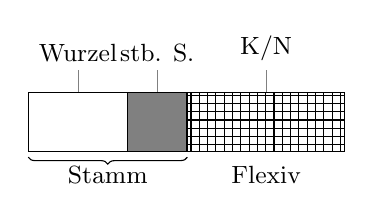
\begin{tikzpicture}[pin distance=2ex]\small
	\node at (0,0) [draw, pin={above:Wurzel}, minimum width=1.25cm, minimum height=0.75cm] (wurzel) {};
	\node [right of=wurzel, anchor=west, node distance=0.625cm, draw, minimum size=0.75cm, pin={above:stb. S.}, fill=black!50] (stbS) {};
	\node [right of=stbS, anchor=west, node distance=0.375cm, draw, pin={above:K/N}, minimum width=2cm, minimum height=0.75cm, pattern=grid] (KN) {};	
	\draw[decorate,decoration={brace,mirror,raise=.5ex}] (wurzel.south west)	-- (stbS.south east) node [midway,below=.5ex] (stamm) {Stamm};
	\path let \p1=(KN),\p2=(stamm) in node at (\x1,\y2) {Flexiv};
\end{tikzpicture} &  & 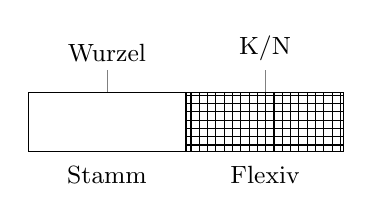
\begin{tikzpicture}[pin distance=2ex]\small
	\node at (0,0) [draw, pin={above:Wurzel}, minimum width=2cm, minimum height=0.75cm] (wurzel) {};
	\node [right of=wurzel, anchor=west, node distance=1cm, draw, pin={above:K/N}, minimum width=2cm, minimum height=0.75cm, pattern=grid] (KN) {};
	\node [below=0.5ex of wurzel] {Stamm};
	\node [below=0.5ex of KN] {Flexiv};
\end{tikzpicture}\\
\lspbottomrule
\end{tabular}
\caption{Dreigliederige Struktur im Indogermanischen und zweigliedrige Substantivstruktur im Germanischen (nach \citealt[47]{Nübling2005} und \citealt[107]{Werner1969})}
\label{tab:4}
\end{table}

Im Germanischen sind die früher separaten stammbildenden Suffixe anders als im Indogermanischen nicht in allen Flexionsformen eines Paradigmas erhalten und werden nicht uniform realisiert. Gleichzeitig entfällt die transparente Motivierung der Klassenbildung, die im Indogermanischen durch das stammbildende Suffix als formale Markierung einer semantischen Differenzierung gegeben war. In der Folge bleibt die formale Varianz, nicht aber die semantische Motiviertheit der Deklinationsklassen erhalten (\tabref{tab:5}, vgl. \citealt[73]{Kürschner2008a}, \citealt[61--67]{Ramat1981}).

\begin{table}
\caption{System der Deklinationsklassen im Germanischen mit Anmerkungen zu Klassengröße, Produktivität und möglichen Ausgleichsprozessen (nach  \citealt{KraheMeid1969, Kürschner2008a, Nübling2008, Ramat1981})}
\label{tab:5}
\begin{subtable}{\textwidth}
\caption{Vokalische Stämme}
\small
\begin{tabularx}{\textwidth}{llllQQ}
\lsptoprule
 {DK} & \multicolumn{3}{c}{{Genus}} & {Beispiele} & {Anmerkungen}\\
\cmidrule(lr){2-4}
              & {F} & {M} & {N} & {Nom.Sg. -- Nom.Pl.} & \\
\midrule
 \textit{a}-Klasse & {}$-$ & + & + & m.*\textit{dagaz} -- *\textit{dagos} ‚Tag‘ & \multirow[t]{2}{=}{große, produktive Klasse}\\
  (idg. \textit{o}{}-Kl.)&  &  &  & n. *\textit{wurða} -- * \textit{wurðo} ‚Wolf\textit{‘} & \\
\tablevspace
 \makecell[tl]{\textit{ja}-Klasse\\(idg. \textit{yo}{}-Kl.)} & {}$-$ & + & + & m.*\textit{harjaz} -- *\textit{harjoz} ‚Heer‘ & \multirow[t]{4}{=}{Subklassen der \textit{a}{}-Klasse mit weniger Mitgliedern, aber ähnlichem Deklinationsmuster}\\
   &  &  &  & n. *\textit{kunja\textsuperscript{n}} -- *\textit{kunjo} ‚Stamm, Geschlecht‘ & \\
\tablevspace
 \makecell[tl]{\textit{wa}-Klasse\\(idg. \textit{wo}{}-Kl.)} & {}$-$ & + & + & m.*\textit{snaiwaz} -- *\textit{snaiwoz/os} ‚Schnee‘ & \\
  &  &  &  & n. *\textit{trewa\textsuperscript{n}} -- *\textit{trewo} ‚Baum‘ & \\
\tablevspace
 \makecell[tl]{\textit{ō}-Klasse\\(idg. \textit{ā}-Kl.)} & + & {}$-$ & {}$-$ & *\textit{wullo} -- *\textit{wulloz} ‚Wolle‘ & große, produktive Klasse\\
\tablevspace
 \makecell[tl]{\textit{jō}-Klasse\\(idg. \textit{ā}-Kl.)} & + & $-$ & $-$ & *\textit{siƀjō} -- *\textit{siƀjōz} ‚Sippe‘ & \multirow[t]{3}{=}{Subklassen der \textit{ō}{}-Klasse mit weniger Mitgliedern, aber ähnlichem Deklinationsmuster}\\
 \tablevspace
 \makecell[tl]{\textit{wō}-Klasse\\(idg. \textit{ā}-Kl.)} & + & {}$-$ & {}$-$ & *\textit{trewwō} -- *\textit{trewwōz} ‚Treue‘ & \\
 & & & & &\\
\tablevspace
 \multirow[t]{3}{*}{\makecell[tl]{\textit{i}-Klasse\\(idg. \textit{i}{}-Kl.)}} & + & + & (+) & f. *\textit{dēðiz} -- \textit{ðedijiz} ‚Tag‘ & \multirow[t]{3}{=}{kleinere Klasse (fast keine Neutra mehr),\footnote{Die „kärglichen Spuren“ \citep[71]{Ramat1981} der Neutra sind nur im Angelsächsischen und Altsächsischen erhalten; im Deutschen sind nur Maskulina und Feminina belegt.} Mischung mit anderen Klassen: Mask. mit \textit{a}{}-Klasse, Fem. mit \textit{ō}{}-Klasse}\\
  &  &  &  & m. *\textit{gastiz} -- *\textit{gastijiz} ‚Gast‘ & \\
  &  &  &  & n. *\textit{mari} -- (-) ‚Meer‘ & \\
  &  &  &  & &\\
  &  &  &  & &\\
\tablevspace
 \multirow[t]{3}{*}{\makecell[tl]{\textit{u}-Klasse\\(idg. \textit{u}{}-Kl.)}} & + & + & {}$-$ & f. *\textit{handuz} -- andere Kl. ‚Hand‘ & \multirow[t]{3}{=}{Feminina bereits ausgeschieden; kleine Klasse, im Abbau befindlich}\\
  &  &  &  & m. *\textit{sunuz} -- *\textit{suniwez} ‚Sohn‘ & \\
  &  &  &  & n. *\textit{fehu} -- (kein Pl.) ‚Vieh‘ & \\
  \lspbottomrule
\end{tabularx}
\end{subtable}
\end{table}

\begin{table}
\ContinuedFloat
\caption{Dreigliederige Struktur im Indogermanischen und zweigliedrige Substantivstruktur im Germanischen (nach \citealt[47]{Nübling2005} und \citealt[107]{Werner1969})}
\begin{subtable}{\textwidth}
\caption{Konsonantische Stämme}
\small
\begin{tabularx}{\textwidth}{llllQQ}
\lsptoprule
 {DK} & \multicolumn{3}{c}{{Genus}} & {Beispiele} & {Anmerkungen}\\
\cmidrule(lr){2-4}
              & {F} & {M} & {N} & {Nom.Sg. -- Nom.Pl.} & \\
\midrule
\multirow[t]{3}{*}{\makecell[tl]{\textit{n}-Klasse\\„schwache“\\Deklination}} & + & + & + & f. *\textit{tungo} -- *\textit{tungon(e)z} ‚Zunge‘ & \multirow[t]{3}{=}{große, hochproduktive Klasse, insb. Konkreta und Belebtes}\\
  &  &  &  & m. *\textit{mēnan} -- *\textit{mēnan(e)z} ‚Mond‘ & \\
  &  &  &  & n. *\textit{herton} -- *\textit{hertōno} Herz‘ & \\
  \tablevspace
 \textit{ī}-Klasse & + & {}$-$ & {}$-$ & *\textit{Þurstī\textsuperscript{n}} -- *\textit{Þurstīnez} ‚Durst‘ & neue Subklasse der \textit{n}{}-Klasse\\
 \tablevspace
 \textit{r}-Klasse  & + & + & {}$-$ & f. *\textit{dūhter} -- \textit{dūhter(i)z} ‚Tochter‘ & \multirow[t]{2}{=}{Kleinstklasse mit Verwandschafts-bezeichnungen; unproduktiv}\\
  &  &  &  & m. *\textit{brōþar} -- \textit{brōþ(e)riz} ‚Bruder‘ & \\
  \tablevspace
 \textit{nd}-Stämme  & {}$-$ & + & {}$-$ & *\textit{frijōnd} -- *\textit{frijōnd(e)z} ‚Freund‘  & kleine Klasse substantivierter Partizipien\\
 \tablevspace
 Wurzelstämme  & + & {}$-$ & {}$-$ & f. *\textit{burgs} -- *\textit{burgiz ‚}Burg‘ &\multirow[t]{2}{=}{kleine Klasse; im Germ. fast nur noch Feminina}\\
  &  &  &  & m. *\textit{mannz} -- *\textit{manniz} ‚Mann‘ & \\
\lspbottomrule
\end{tabularx}
\end{subtable}
\end{table}

Infolge der Reanalyse des stammbildenden Suffixes als Teil des Flexivs und der Verschiebung der Morphemgrenzen fallen Wurzel und Stamm formal zusammen. Der typologische Wandel von der Stamm- zur Grundformflexion ist im Germanischen indes noch nicht vollzogen, sowohl das Indogermanische als auch das Germanische sind stammflektierende Sprachen. Das Kasus/Numerus-Allomorph wird nicht -- wie beim grundformflektierenden Verfahren -- additiv an den Stamm gefügt, sondern ein Allomorph wird durch ein anderes ersetzt (vgl. \citealt[295]{Nübling2008}, \citealt[106]{Werner1969}). Im Germanischen besteht somit noch keine Opposition zwischen unmarkiertem Nom.Sg. und markiertem Nom.Pl., sondern auch das Singularparadigma weist (in stärkerem Maße als spätere Sprachstufen des Deutschen) distinkte Flexive auf (vgl. \citealt[76]{Kürschner2008a}). Der typologische Wandel von der Stamm- zur Grundformflexion setzt im Althochdeutschen ein. Mit Ausnahme der \textit{ō}{}-Deklination (Nom./Akk./Gen.Sg. \textit{gëba}, Dat.Sg. \textit{gëbu} ‚Gabe‘) weisen die übrigen starken Deklinationsklassen bereits eine unsuffigierte Grundform im Nom.Sg. auf (\tabref{tab:6}, vgl. \citealt[81]{Kürschner2008a}, anders \citealt{Harnisch1994b, Harnisch2001}).

\begin{table}
\small
\begin{tabularx}{\textwidth}{lllllll}
\lsptoprule

\multicolumn{2}{l}{germ. DK} & {mask. \textit{a}} & {neutr. \textit{a}} & {fem. \textit{ō}} & {mask. \textit{i}} & {fem. \textit{i}}\\
\multicolumn{2}{c}{} & \textit{tag}  & \textit{wort}  & \textit{gëba}  & \textit{gast}  & \textit{anst} \\
& & ‚Tag‘ & ‚Wort‘ &  ‚Gabe‘ &  ‚Gast‘ &  ‚Gunst‘\\
\midrule
{Sg.} & Nom./Akk. & \textit{tag} & \textit{wort} & \textit{gëba} & \textit{gast} & \textit{anst}\\
& Gen. & \textit{tages (-as)} & \textit{wortes} & \textit{gëba} & \textit{gastes} & \textit{ensti}\\
& Dat. & \textit{tage (-a)} & \textit{worte (-a)} & \textit{gëbu} & \textit{gaste} & \textit{ensti}\\
& Instr. & \textit{tagu, -o} & \textit{wortu} & \textit{{}--} & \textit{gestiu}>\textit{gastiu} & \textit{{}--}\\
\tablevspace
{Pl.} & Nom./Akk. & \textit{taga} & \textit{wort} & \textit{gëba} & \textit{gesti} & \textit{ensti}\\
& Gen. & \textit{tago} & \textit{worto} & \textit{gëbōno} & \textit{gesteo/-io>gesto} & \textit{ensto}\\
& Dat. & \textit{tagum} & \textit{wortum} & \textit{gëbōm} & \textit{gestim} & \textit{enstim}\\
\lspbottomrule
\end{tabularx}
\caption{Starke Deklinationsklassen des Althochdeutschen (nach \citealt{BrauneHeidermanns2018})}
\label{tab:6}
\end{table}

Kasus und Numerus werden in dieser Phase weiterhin durch ein Portmanteau-Morphem, d.\,h. durch ein fusioniertes Kasus/Numerus-Suffix, markiert. Im Althochdeutschen setzt dann die Separierung des Kasus/Numerus-Ausdrucks ein, Numerusprofilierung und Kasusnivellierung als die beiden zentralen Tendenzen des nominalmorphologischen Wandels im Deutschen werden eingeleitet (vgl. \citealt[§192a]{BrauneHeidermanns2018}). Entscheidend bei dieser Entwicklung ist ein phonologischer Wandel, der den morphologischen Wandel anstößt: der \textit{i}-Umlaut. Im Althochdeutschen führt ein zunächst rein phonologischer Prozess der Vokalassimilation zu innerparadigmatischen Alternationen zwischen palatalen und nicht-palatalen Vokalen. Ein /i/ oder /j/ in der Folgesilbe lösen eine regressive assimilatorische Palatalisierung eines hinteren Vokals aus, z.\,B. ahd. \textit{apful} ‚Apfel‘ -- \textit{epfili} ‚Äpfel‘, ahd. \textit{tag} ‚Tag‘ -- \textit{tegelih} ‚täglich‘ (vgl. \citealt[§51]{BrauneHeidermanns2018}, \citealt[229]{Wiese1987}). Die erste Phase des \textit{i}{}-Umlauts betrifft vor allem die mask. und fem. \textit{i}{}-Klassen und die neutr. \textit{iz/az}{}-Klasse, die jeweils \textit{i}{}-haltige Kasus/Numerus-Suffixe aufweisen. Strukturell sind die palatalisierten Umlautprodukte zunächst Allophone der velaren Vokale, bevor die Phonemisierung erfolgt und in einer Erweiterung des Vokalphoneminventars resultiert (vgl. \citealt[195]{Ronneberger-Sibold1990}, \citealt[120--123]{Schulze2016}, \citealt[306]{Sonderegger1979}). Zwei Prozesse, die auf die beiden ahd. Umlautphasen\footnote{Beim sogenannten Primär\-umlaut im Althochdeutschen wird nur die Palatalisierung von /a/ auch systematisch verschriftlicht. Der sogenannte Sekundär\-umlaut, das heißt die Verschriftlichung der übrigen palatalisierten Vokale, die zwar schon im Althochdeutschen eingetreten ist, wird meist erst auf das Mittelhochdeutsche datiert, vgl. ahd. \textit{hūsir} [hyːsir] > mhd. \textit{hiuser} [hyːsər]. Aktueller Forschungsstand ist nach \citet[16]{Nübling2013}, dass Primär- und Sekundär\-umlaut gleichzeitig stattgefunden haben.} folgen, leiten den Übergang vom phonologischen zum morphologischen Umlaut ein: der phonologische Prozess der Vokalreduktion in den Endsilben und der morphologische Prozess des innerparadigmatischen Ausgleichs.

Im Übergang vom Alt- zum Mittelhochdeutschen werden die Vollvokale in den Endsilben zu Schwa reduziert, das umlautauslösende /i/ verschwindet aus den Suffixen und damit auch der Auslöser eines rein phonologischen Umlauts: ahd. \textit{gesti} > \textit{geste} ‚Gäste‘. \citet[235]{Wiese1987} sieht in der Endsilbenabschwächung die Grundlage zur Reanalyse der Wortformen. Nach dem Schwund des /i/ als Auslöser der Vokalharmonie wird das „Harmoniemerkmal“ als Teil des Stammes reanalysiert und der Umlaut mit einem morphologischen Verfahren wie z.\,B. Pluralmarkierung assoziiert (siehe auch \citealt[68--69]{Wurzel1982}). \citet[60]{Wurzel1982} hingegen sieht in den im Althochdeutschen einsetzenden innerparadigmatischen Ausgleichsprozessen den Beginn einer Morphologisierung des Umlauts. Lautgesetzlich entstandene Umlaute scheiden aus dem Singularparadigma aus, obwohl das /i/ in der Folgesilbe und damit die phonologische Umgebung, die den Umlaut auslöst, erhalten bleibt, vgl. Gen./Dat.Sg. \textit{henin} > \textit{hanin} ‚Hahn‘ (\tabref{tab:7}, vgl. \citealt[71--72]{Dammel2018}, \citealt[308--309]{Sonderegger1979}).\footnote{Die Singular-Suffix-Variante -\textit{in} findet sich (neben -\textit{en}) im Oberdeutschen, sowie im Ost- und Rheinfränkischen (vgl. \citealt[1179]{Sonderegger2000}). Das \textit{i}{}-haltige Suffix bewirkte im Singular den Umlaut, der später jedoch wieder eliminiert wurde; bereits im 9. Jhd. sind die nichtumgelauteten Singularformen die Regel (vgl. \citealt[§221]{BrauneHeidermanns2018}).} Das Deklinationsparadigma von ahd. \textit{hano} ‚Hahn‘ aus der mask. \textit{n}{}-Klasse zeigt hier zudem, dass der Pluralumlaut keine Voraussetzung war, um den Kasusumlaut im Gen./Dat.Sg. zu tilgen, sondern dass die Tilgung durch fehlende Uniformität im Bereich des Stammvokalismus im Singularparadigma bedingt war (vgl. \citealt[49--50]{Nübling2005}). Im Ergebnis stehen sich umlautlose Singularformen und (bis hierhin rein lautgesetzlich entstandene) Pluralumlaute im Paradigma gegenüber. Im Übergang vom Mittelhochdeutschen zum Frühneuhochdeutschen folgt die analogische Ausweitung des Pluralumlauts; der Übergang einer phonologisch bedingten Alternation zu einem produktiven morphologischen Marker ist vollzogen. In diesem Zusammenhang ist der Umlaut auch typologisch von Bedeutung, da die flexivische Information in den Stamm eindringt und damit im Althochdeutschen der Wandel von einem bis dahin rein additiven Kasus/Numerus-Ausdruck hin zur stammaffizierenden Kodierung flexivischer Information einsetzt (vgl. \citealt[48]{Nübling2005}, \citealt[182]{Seiler2008}, \citealt[1691]{Solms2004}). Infolge der Tilgung der lautgesetzlichen Umlaute aus dem Singularparadigma ist dieses morphophonologische Verfahren für die Numerusmarkierung reserviert.

\begin{table}
\begin{tabular}{lllll}
\lsptoprule
&  & \multicolumn{2}{c}{{\textit{iz}/\textit{az}{}-Klasse}} & \makecell[tl]{{mask. \textit{n}{}-}{Deklination}}\\
\cmidrule(lr){3-4}
&  & {Vorahd.} & {Ahd.} & \\
\midrule
{Sg.} & {Nom.} & {\textit{*lamb}} & {\textit{lamb}} & \textit{hano}\\
& {Gen.} & \textit{*lamb-ir-as} & \textit{l\textbf{e}mb-ir-es} $>$ \textbf{\textit{lambes}} & \textit{h\textbf{e}nin} $>$ \textbf{\textit{hanin}}\\
& {Dat.} & {\textit{*lamb-ir-a}} & {\textit{l\textbf{e}mb-ir-e} $>$ \textbf{\textit{lambe}}} & \textit{h\textbf{e}nin} $>$ \textbf{\textit{hanin}}\\
& Akk. & \textit{*lamb} & \textit{lamb} & \textit{hanon}\\
\tablevspace
{Pl.} & {Nom.} & {\textit{*lamb-ir-u}} & {\textit{l\textbf{e}mb-ir}} & \textit{hanon}\\
& Gen. & \textit{*lamb-ir-o} & \textit{l\textbf{e}mb-ir-o} & \textit{hanōno}\\
& {Dat.} & {\textit{*lamb-ir-um}} & {\textit{l\textbf{e}mb-ir-um}} & \textit{hanōm}\\
& Akk. & \textit{*lamb-ir-u} & \textit{l\textbf{e}mb-ir} & \textit{hanon}\\
\lspbottomrule
\end{tabular}
\caption{Paradigma von ahd. \textit{lamb} (\textit{iz/az}{}-Klasse) und ahd. \textit{hano} (mask. \textit{n}{}-Deklination, vgl. \citealt{BrauneHeidermanns2018}, \citealt[84]{Kürschner2008a}, \citealt[49]{Nübling2005}, \citealt[60]{Wurzel1982})\label{tab:7}}
\end{table}

\tabref{tab:7} weist für die neutr. \textit{iz/az}{}-Klasse einen weiteren innerparadigmatischen Ausgleich aus. Im Althochdeutschen ist das frühere stammbildende Suffix \mbox{-\textit{ir}} im Singularparadigma im Nominativ/Akkusativ lautgesetzlich getilgt, im Gen./Dat.Sg. ist es erhalten. Zu diesem Zeitpunkt hat -\textit{ir} die Funktion als transparenter Deklinationsklassenmarker bereits verloren, da es nicht mehr uniform im Paradigma vorkommt. Das vormals stammbildende Suffix wird in der Folge nicht mehr als Teil des Stammes interpretiert, sondern als Pluralmarker reanalysiert und gleichzeitig im Gen./Dat.Sg. getilgt (vgl. \citealt[50]{Nübling2005}, \citealt[87--89]{Wegener2005}). Als Ergebnis der Eliminierung von Umlaut (UL) und \textit{ir}{}-Suffix aus dem Singularparadigma erscheint der Singular als unmarkierte Basiskategorie, die Pluralinformation wird formal durch UL+\textit{ir} markiert (vgl. \citealt[51]{Nübling2005}, \citealt[1691]{Solms2004}). Damit ist im Paradigma der \textit{iz/az}{}-Deklination der Übergang von der Stamm- zur Grundformflexion vollzogen, die Nominativ-Singular-Form ist formal vollständig im Plural enthalten. Gleichzeitig hat die Separierung von Kasus/Numerus-Ausdruck zur spezifischen Reihenfolge von Numerus- und Kasusmarker geführt, die auch im Neuhochdeutschen wirksam ist: Auf das Pluralallomorph \mbox{-\textit{ir}} folgt der Kasusmarker in Gen.Pl. \textit{lemb-ir-o}, Dat.Pl. \textit{lemb-ir-um} (vgl. nhd. \textit{Lämm-er-n}). Mit der Separierung des Kasus/Numerus-Ausdrucks und der Reanalyse von Umlaut und früherem Kasus/Numerus-Suffix zu Pluralmarkern setzen in der \textit{iz/az}{}-Klasse im Althochdeutschen jene Umstrukturierungen des Deklinationssystems ein, die diachron zu einer Profilierung der Numeruskategorie und zu einem Abbau der Kasusmarkierung am Substantiv führen (vgl. \citealt[195--199]{DammelGillmann2014}, \citealt[85]{Kürschner2008a}).\pagebreak

Einen weiteren Beitrag zu Numerusprofilierung und Kasusnivellierung leistet die Endsilbenabschwächung. Die vollvokalischen Flexionssuffixe des Althochdeutschen sind von diesem Wandel besonders betroffen, da die Vokalqualität als formaler Marker von flexivischen Distinktionen funktionalisiert ist (vgl. \citealt[80]{Kürschner2008a}, \citealt[1172]{Sonderegger2000}). \citet[109]{Werner1969} zählt sechs ahd. Pluralallomorphe (\textit{∅}, -\textit{a}, -\textit{e}, \textit{i}, -\textit{un}, -\textit{ir}). Die Vollvokalqualität der Suffixe wird im Übergang zum Mittelhochdeutschen zu einem uniformen Schwa reduziert, so werden beispielsweise das Allomorph -\textit{a} in ahd. Nom./Akk.Pl. \textit{tag-a} ‚Tag‘ und das Allomorph -\textit{o} im Gen.Pl. \textit{tag-o} zu Schwa (Nom./Akk./Gen.Pl. \textit{tag-e}) reduziert (\tabref{tab:8}). \citet[246]{Sonderegger1979} beziffert die Reduktion der segmentierbaren Flexive von 52 auf 16 im Mittelhochdeutschen. Im Ergebnis dieses phonologischen Prozesses erscheinen verstärkt synkretische Formen im Pluralparadigma, es entsteht „ein strukturell grundsätzlich neues Flexionssystem“ \citep[1691]{Solms2004}. Im Fall der fem. \textit{ō}{}-Klasse führt die Vokalreduktion endgültig zu einer Ablösung des stammflektierenden Verfahrens durch die Grundformflexion. Die Differenzierung von Nom.Sg. \textit{gëba} vs. Dat.Sg. \textit{gëbu} durch Kontraste im Vokalismus entfällt, im Singularparadigma erscheint ein einheitliches Schwa in der Reduktionssilbe (\textit{gebe}) und wird als Teil des Stammes reanalysiert (vgl. \citealt[87]{Kürschner2008a}).


\begin{sidewaystable}
\small
\begin{tabular}{ *{14}{l} }
\lsptoprule
\multicolumn{2}{c}{germ. DK} & \multicolumn{2}{c}{mask. \textit{a}} & \multicolumn{2}{c}{neutr. \textit{a}} & \multicolumn{2}{c}{fem. \textit{ō}} & \multicolumn{2}{c}{mask. \textit{i}} & \multicolumn{2}{c}{fem. \textit{i}} & \multicolumn{2}{c}{neutr. \textit{iz/az}}\\
\cmidrule(lr){3-4}\cmidrule(lr){5-6}\cmidrule(lr){7-8}\cmidrule(lr){9-10}\cmidrule(lr){11-12}\cmidrule(lr){13-14}
\multicolumn{2}{c}{} & \textit{tac}  & Ahd. & \textit{wort}  & Ahd. & \textit{gebe}  & Ahd. & \textit{gast}  & Ahd. & \textit{kraft}  & Ahd. & \textit{lamp}  & Ahd.\\
\multicolumn{2}{c}{} & ‚Tag‘ & & ‚Wort‘ & & ‚Gabe‘ & & ‚Gast‘ & & ‚Kraft‘ & & ‚Lamm‘ & \\\midrule
Sg. & N./A. & \textit{tac} & \textit{∅} & \textit{wort} & \textit{∅} & \textit{geb\textbf{e}} & \textit{a} & \textit{gast} & \textit{∅} & \textit{kraft} & \textit{∅} & \textit{lamp} & \textit{∅}\\
& G. & \textit{tag\textbf{es}} & \textit{es} & \textit{wort\textbf{es}} & \textit{es} & \textit{geb\textbf{e}} & \textit{a} & \textit{gast\textbf{es}} & \textit{es} & \textit{kr\textbf{e}}\textit{ft\textbf{e}} & \textit{UL+i} & \textit{lamb\textbf{es}} & \textit{es}\\
& D. & \textit{tag\textbf{e}} & \textit{e} & \textit{wort\textbf{e}} & \textit{e} & \textit{geb\textbf{e}} & \textit{u} & \textit{gast\textbf{e}} & \textit{e} & \textit{kr\textbf{e}}\textit{ft\textbf{e}} & \textit{UL+i} & \textit{lamb\textbf{e}} & \textit{e}\\
Pl. & N./A. & \textit{tag\textbf{e}} & \textit{a} & \textit{wort} & \textit{∅} & \textit{geb\textbf{e}} & \textit{a} & \textit{g\textbf{e}}\textit{st\textbf{e}} & {\textit{UL}}\textit{+i} &  \textit{kr\textbf{e}}\textit{ft\textbf{e}} & \textit{UL+i}  & \textit{l\textbf{e}}\textit{mb\textbf{er}} & {\textit{UL}}\textit{+ir}\\
& G. & \textit{tag\textbf{e}} & \textit{o} & \textit{wort\textbf{e}} & \textit{o} & \textit{geb\textbf{en}} & \textit{ōno} & \textit{g\textbf{e}}\textit{st\textbf{e}} & {\textit{UL}}\textit{+o} & \textit{kr\textbf{e}}\textit{ft\textbf{e}} & {\textit{UL}}\textit{+o} & \textit{l\textbf{e}}\textit{mb\textbf{er}} & {\textit{UL}}\textit{+iro}\\
& D. & \textit{tag\textbf{en}} & \textit{um} & \textit{wort\textbf{en}} & \textit{um} & \textit{geb\textbf{en}} & \textit{ōm} & \textit{g\textbf{e}}\textit{st\textbf{en}} & {\textit{UL}}\textit{+im} & \textit{kr\textbf{e}}\textit{ft\textbf{en}} & {\textit{UL}}\textit{+im} & \textit{l\textbf{e}}\textit{mb\textbf{ern}} & {\textit{UL}}\textit{+irum}\\
\tablevspace
\multicolumn{2}{c}{\makecell[tl]{Gen.Sg.-/\\Plural-\\flexiv}} & \multicolumn{2}{c}{ \textit{{}-(e)s/-e}} & \multicolumn{2}{c}{\textit{-(e)s/-∅}} & \multicolumn{2}{c}{\textit{∅/∅}} & \multicolumn{2}{c}{\textit{{}-(e)s/UL+e}} & \multicolumn{2}{c}{\textit{UL+e/UL+e}} & \multicolumn{2}{c}{ \textit{{}-(e)s/(UL)+er}}\\
\lspbottomrule
\end{tabular}
\caption{Starke mhd. Deklinationsklassen mit Bezug zu den germ. Deklinationsklassen und zum jeweiligen Kasus/Numerus-Allomorph im Althochdeutschen (vgl. \citealt{KleinEtAl2018}, \citealt{Kürschner2008a})\label{tab:8}}
\end{sidewaystable}

Dieser formale Wandel der Flexionssuffixe erfolgt dabei -- zumindest aus flexionsmorphologischer Perspektive -- unsystematisch. In den einzelnen Klassen fallen bedingt durch den phonologischen Prozess der Vokalreduktion unterschiedliche Suffixe zusammen und führen zu spezifischen Paradigmenausprägungen (vgl. \citealt[86]{Kürschner2008a}). Nur im Dat.Pl. führt die Uniformierung des Flexivs im Spätalthochdeutschen zu -\textit{(e)n} zu einem einheitlichen Marker in sämtlichen starken Deklinationsklassen (vgl. Dat.Pl. \textit{tage-n} ‚Tag‘, \textit{wort-en} ‚Wort‘, \textit{krefte-n} ‚Kraft‘). Damit setzt sich die Abfolge von Numerus- und Kasus-Ausdruck, die sich im Althochdeutschen bereits in der \textit{iz/az}{}-Klasse herausgebildet hat, im mhd. Deklinationssystem durch. Auf den Stamm folgt die Markierung der Nu"-me"-rus- und anschließend der Kasusinformation (vgl. \citealt[87--88]{Kürschner2008a}, \citealt[51--52]{Nübling2005}).

Die phonologisch und morphologisch bedingten Umstrukturierungen des Deklinationssystems und der morphophonologische Wandel der Allomorphe führen diachron auch zu einem Wandel der Exponenz der Deklinationsklassen. Zum einen ist die Klassenzuordnung auf Basis ihrer primär semantischen Konditionierung und infolge der Fusion von Kasus/Numerus-Flexiv und des stammbildenden Suffixes, das -- wenngleich nicht mehr uniform im Paradigma vorhanden -- auch im Althochdeutschen teilweise noch transparent ist, infolge der Vokalreduktion zu Schwa nicht mehr möglich. In der Folge manifestiert sich Deklinationsklasse durch klassenspezifische Allomorphe und Paradigmenkonstellationen, wobei sich deklinationsklassenspezifische Marker auf wenige Stellen im Paradigma zurückziehen. Durch den Abbau der Kasusmarkierung am Substantiv wird die Pluralallomorphie zum primären Unterscheidungsmerkmal von Deklinationsklassen, Kasusexponenz im Gen.Sg. ist nur noch sekundäres Merkmal (vgl. \citealt[71]{KleinEtAl2018}). In einigen germanischen Sprachen und auch in den Dialekten des Deutschen, in denen der Abbau der Kasusmarkierung noch weiter vorangeschritten ist, manifestieren sich Deklinationsklassen einzig in der Pluralallomorphie (so z.\,B. im Dänischen und Schwedischen, vgl. \citealt{DammelEtAl2010}).

\subsection{Aus- und Umbau der Deklinationsklassen}
\label{sec:3.1.2}
Im Zentrum der bisherigen Darstellung stand der Aspekt des Deklinationsklassenwandels, d.\,h. der Wandel des Ausdrucks der Kategorie Deklinationsklasse. Im Fokus des folgenden Kapitels stehen (1) das Inventar der Deklinationsklassen und (2) die (Re-)Organisation des Deklinationsklassensystems in Form von Ausbau, Schwund und Deklinationsklassenwechsel. Die zentralen Entwicklungen in den einzelnen Sprachstufen des Deutschen sind im Folgenden zusammengefasst.

Diachron findet in der Tendenz ein Abbau von Deklinationsklassen statt. Infolge der phonologisch und morphologisch bedingten Umstrukturierungen (insbesondere durch den \textit{i}{}-Umlaut) nimmt die Komplexität des Deklinationsklassensystems bis zum Althochdeutschen noch zu. Doch die Separierung des Kasus\slash Numerus-Ausdrucks, die Reanalyse als Pluralmarker und der damit einhergehende Wandel der Deklinationsklassenexponenz leiten -- neben der Endsilbenabschwächung -- den Abbau von Deklinationsklassen und damit eine Reduktion des Deklinationsklassensystems ein (vgl. \citealt[293]{DammelKürschner2018}).

Daneben führen Deklinationswechsel zur Auflösung kleinerer Klassen. Deklinationsklassenwechsel ist dabei in vielen Fällen durch verschiedene außerflexivische Faktoren, allen voran Genus und semantische Merkmale, bedingt (siehe auch \sectref{sec:3.2}). Bereits im Germanischen vollziehen sich Umstrukturierungen des Deklinationsklassensystems, die stark durch Genus gesteuert sind (vgl. \citealt[74--77]{Kürschner2008a}, \citealt[296--297]{Nübling2008}):

\begin{itemize}
\item In der fem. und mask. \textit{i}-Klasse findet eine Differenzierung der Flexion statt: Die Maskulina nehmen im Singularparadigma die Formenbildung der mask. \textit{a}{}-Klasse an, die Feminina verändern die Formenbildung nicht.
\item Die Entsprechungen der \textit{a}{}- und der \textit{ō}{}-Klasse im Indogermanischen weisen Klassenmitglieder aller drei Genera auf, im Germanischen scheiden die Feminina aus der \textit{a}{}-Klasse, Maskulina und Neutra hingegen aus der \textit{ō}-Klasse aus. Im Ergebnis stehen sich die fem. \textit{ō}-Klasse und die mask./neutr. \textit{a}-Klasse gegenüber.
\end{itemize}

Im Übergang vom germ. zum ahd. Deklinationssystem besteht infolgedessen bei den vokalischen Stämmen eine Genusschranke zwischen Femininum und Nicht-Femininum, die konsonantischen Stämme (mit Ausnahme der \textit{n}{}-Klasse) setzen sich aus Maskulina und Feminina zusammen (vgl. \tabref{tab:5}, \citealt[77]{Kürschner2008a}, \citealt[§3]{Paul1968}).

Im Althochdeutschen findet eine Reduktion der germ. Klassen statt, indem kleinere Klassen in größere übertreten, so etwa die mask. \textit{u}{}-Stämme in die \textit{i}{}-Klasse, bei den Feminina geht die Subklasse der \textit{wō}{}-Stämme in die übergeordneten \textit{ō}{}-Klasse auf (vgl. \tabref{tab:9}). Mit dem Wechsel der mask. \textit{nd}{}- und \textit{er}{}-Klasse, beide konsonantische Stämme, in die vokalische mask. \textit{a}{}-Klasse wird die aus dem Indogermanischen ererbte Einteilung in konsonantische und vokalische Stämme aufgegeben, die sich historisch aus der Form des stammbildenden Suffixes ergab, z.\,B. für die \textit{er}{}-Stämme germ. *\textit{brōþar} -- \textit{brōþ(e)riz} ‚Bruder‘ > spätahd. \textit{bruoder} -- \textit{bruodera} ‚Bruder‘ und -- bereits im älteren Althochdeutschen -- \textit{fater} -- \textit{fatera} ‚Vater‘ (vgl. \citealt[§235]{BrauneHeidermanns2018}, \citealt[75]{Kürschner2008a}). Infolgedessen besteht ein Unterscheidungsmerkmal der Formenbildung im ahd. Deklinationssystem zwischen starker und schwacher Deklination. Die schwache Deklination, die auf die germ. \textit{n}{}-Stämme zurückgeht, weist im Plural und in den obliquen Kasus auf Nasal auslautende Flexionssuffixe auf, während die Flexive der starken Deklination nicht auf Nasal auslauten und auch sonst kein gemeinsames phonologisches Merkmal aufweisen (vgl. \citealt[304--305]{Fortson2007}, \citealt[80]{Kürschner2008a}).\footnote{Eine Ausnahme bilden hier die Neutra, die im Akk.Sg. kein Nasalsuffix aufweisen: Nom.\slash Akk.Sg. ahd. \textit{ouga} -- Gen./Dat. \textit{ougen} ‚Auge‘ (\citealt[§224]{BrauneHeidermanns2018}, vgl. \citealt[85]{Kürschner2008a}).}

\begin{table}
\tabcolsep=.75\tabcolsep
\fittable{\begin{tabular}{llll}
\lsptoprule
Germanisch & Althochdeutsch & Mittelhochdeutsch & Neuhochdeutsch\\
\midrule
mask. \textit{wa} & {}-\textit{o} / -\textit{wes} / -\textit{wa} & {}-\textit{wes} / -\textit{we} & {}-\textit{s} / -\textit{(e)}\\
\cellcolor{lsLightGray}mask. \textit{a} & {}-\textit{es} / -\textit{a} & {}-\textit{es} / -(\textit{e}) & -\textit{s} / -\textit{(e)}\\
mask. \textit{nd} & -\textit{es} / -\textit{a} & -\textit{es} / -(\textit{e}) & -\textit{s} / -\textit{(e)}\\
\cellcolor{lsLightGray}mask. \textit{er} & -\textit{es} / -\textit{a} & {}-\textit{s} / UL & {}-\textit{s} / UL\\
mask. \textit{ja} & {}-\textit{i} / -\textit{es} / -\textit{e} & {}-\textit{s} / ∅ & {{}-\textit{s} / [UL (Mask.)] -\textit{(e)}}\\
\cellcolor{lsLightGray}neutr. \textit{a} & {}-\textit{es} / ∅ & {}-\textit{es} / ∅ & -\textit{s} / [UL (Mask.)] -\textit{(e)}\\
neutr. \textit{ja} & {}-\textit{i} / -\textit{es} / -\textit{i} & -\textit{es} & -\textit{s} / [UL (Mask.)] -\textit{(e)}\\
neutr. \textit{wa} & {}-\textit{o} / -\textit{wes} / -\textit{o} & {}-\textit{wes} / ∅ & -\textit{s} / [UL (Mask.)] -\textit{(e)}\\
\cellcolor{lsLightGray}fem. \textit{er} & ∅ / ∅ & ∅ / UL & ∅ / UL\\
\cellcolor{lsLightGray}mask. \textit{i} & {}-\textit{es} / UL-\textit{i} & {}-\textit{es} / UL -\textit{e} & {}-\textit{s} / UL -\textit{(e)}\\
mask. \textit{u} & -\textit{es} / UL-\textit{i} & -\textit{es} / UL -\textit{e} & -\textit{s} / UL -\textit{(e)}\\
mask. Wurzelnomina & ∅ / ∅ & -\textit{es} / UL -\textit{e} & -\textit{s} / UL -\textit{(e)}\\
\cellcolor{lsLightGray}fem. \textit{i} & (UL) -\textit{i} / (UL) -\textit{i} & ∅ / (UL) -\textit{e} & ∅ / UL -\textit{e}\\
fem. Wurzelnomina & ∅ / ∅ & ∅ / (UL) -\textit{e} & ∅ / UL -\textit{e}\\
\cellcolor{lsLightGray}fem. \textit{ō} & {}-\textit{a} /-\textit{a} / -\textit{a} < -\textit{ā} & ∅ / ∅ & ∅ / -\textit{(e)n}\\
fem. \textit{wō} & -\textit{a} /-\textit{a} / -\textit{a} < -\textit{ā}& ∅ / ∅ & ∅ / -\textit{(e)n}\\
fem. \textit{jō} & {}-\textit{ea} / -\textit{ea} / -\textit{ea} < -\textit{eā} & ∅ / ∅ & ∅ / -\textit{(e)n}\\
\cellcolor{lsLightGray}fem. \textit{n} & {}-\textit{a} / -\textit{ûn} / -\textit{ûn} & {}-\textit{n} / -\textit{n} & ∅ / -\textit{(e)n}\\
\cellcolor{lsLightGray}mask. \textit{n} & {}-\textit{o} / -\textit{en} / -\textit{on} & -\textit{n} / -\textit{n} & {}-\textit{(e)n} /-\textit{(e)n}\\
\cellcolor{lsLightGray}neutr. \textit{n} & {}-\textit{a} / -\textit{en} / -\textit{un} & -\textit{n} / -\textit{n} & {}-\textit{s} / -\textit{(e)n}\\
\cellcolor{lsLightGray}neutr. \textit{iz/az} & {}-\textit{es} / -\textit{ir} & {}-\textit{es} / UL -\textit{er} & {}-\textit{s} / UL -\textit{er}\\
\multicolumn{3}{c}{} & {}-\textit{s} / -\textit{s} (Mask, Neutr.)\\
 &  &  & ∅ / -\textit{s} (Fem.)\\
\lspbottomrule
\end{tabular}}
\caption{Formale Entwicklung der Deklinationsklassen vom Germanischen zum Neuhochdeutschen (nach \citealt[94]{Kürschner2008a})\protect\footnote{Grau hinterlegt sind die großen, in der Sprachgeschichte prägenden Klassen des germ. Deklinationsklassensystems, die den Referenzpunkt der dialektologischen Darstellung (\chapref{chap:7}) bilden; die Unterklassen (\textit{ja}/\textit{wa} in der \textit{a}{}-Klasse und \textit{jō}/\textit{wō} in der \textit{ō}{}-Klasse) und kleinere Klassen werden im Folgenden ausgeblendet. Die formalen Ausprägungen der Klassen werden jeweils in der Form \textit{Gen.Sg.\slash Nom.Pl.} dargestellt, im Althochdeutschen wird bei erhaltener Stammflexion außerdem das Allomorph des Nom.Sg. angegeben (d.\,h. \textit{Nom.Sg.\slash Gen.Sg.\slash Nom.Pl.}). Die nhd. Klasseneinteilung basiert auf der Klassifikation von \citet[94]{Kürschner2008a}, da diese die diachronen Klassenbewegungen und die Reorganisation des Systems veranschaulicht. Im Neuhochdeutschen sind Pluralallomorphe zu Klassen zusammengefasst, die komplementär verteilt und durch die prosodische Struktur des Stammes konditioniert sind, z.\,B +/$-$ \textit{e}{}-Suffix (Notation „(\textit{e})“). Der Umlaut als Pluralmarker wird dann ohne Klammer angegeben, wenn er bei nicht-palatalem Stammvokalen („umlautbaren Stämmen“, vgl. \citealt[94, FN 27]{Kürschner2008a}) obligatorisch ist; die Notation „(UL)“ verweist auf Pluralformen mit potenziell „umlautbarem“ Stamm aber ohne Umlaut im Plural. Auch die Notation „[UL]“ verweist auf eine komplementäre Klasse mit Umlautplural.}\label{tab:9}}
\end{table}

Im Mittelhochdeutschen setzt sich die Reduktion der historischen Deklinationsklassen fort. Bedingt durch die Endsilbenabschwächung weist die schwache Deklination ein uniformes Nasalsuffix auf, die genusspezifische Differenzierung der Allomorphe durch Vollvokalismus in den Flexiven entfällt lautgesetzlich. Gleichermaßen durch die Endsilbenabschwächung bedingt geht Schwa-Suffix aus den vokalischen Allomorphen vor allem in der ahd. \textit{a}{}- und \textit{i}"=Deklination hervor (Nom.Pl. ahd. \textit{taga} > mhd. \textit{tage} ‚Tage‘, ahd. \textit{krefti} > \textit{krefte} ‚Kräfte‘). Mit der Schwa-Apokope greift erneut ein phonologischer Prozess in das Flexionssystem ein, der vor allem in den apokopierenden obd. Dialekten zu einer Reorganisation des Deklinationssystems führt (vgl. \sectref{sec:4.2.1}). Bei den historischen mask. {\textit{a}}- und {\textit{i}}{}-Klassen sind apokopierte, d.\,h. endungslose, Pluralformen im 12. Jahrhundert nur vereinzelt belegt, im 14. Jahrhundert beträgt der Anteil im Bair. nach \citet[136]{KleinEtAl2018} dagegen 65 \%. Früher und stärker tritt die Apokope bei Mehrsilbern mit Reduktionssilbe -\textit{en}, -\textit{er} und -\textit{el} ein, z.\,B. Nom.Pl. mhd. \textit{nagele} > \textit{nagel} ‚Nägel‘ (vgl.
\citealt[137]{KleinEtAl2018}).

Der Abbau von Nullpluralen, der in einigen wenigen ahd. Deklinationsklassen vorkommt, erfolgt im Mittelhochdeutschen „zunächst noch zaghaft“ (\citealt[135]{KleinEtAl2018}, vgl. \citealt[201]{DammelGillmann2014}, \citealt[89]{Kürschner2008a}, \citealt[1544]{WegeraSolms2000}):

\begin{itemize}
\item Die neutr. \textit{a}{}-Klasse (Typ \textit{wort} -- \textit{wort}) wechselt in das Flexionsmuster der historischen \textit{iz/az-}Klasse\footnote{\citet[153]{KleinEtAl2018} führen bereits für den ahd. Abrogans Belege von historischen neutr. \textit{a}{}-Stämmen an, die das \textit{ir}{}-Flexiv der \textit{iz/az}{}-Klasse angenommen haben: ahd. \textit{feld(h)ir} ‚Felder‘, ahd. \textit{harir} ‚Haare‘ (vgl. \citealt[293]{Nübling2008}). Damit war das historische stammbildende Suffix -\textit{ir}{}- zu diesem Zeitpunkt als Pluralmarker reanalysiert und produktiv.}  (nhd. \textit{Wörter}) oder nimmt das \textit{e}{}-Suffix an (nhd. \textit{Worte}), das bisher ein spezifisches Verfahren der Maskulina war. Die analoge Ausweitung des \textit{e}{}-Suffixes auf die neutr. \textit{a}{}-Klasse vollzieht sich vor allem im Mitteldeutschen, im obd. Sprachraum wirkt die einsetzende Schwa-Apokope der Ausbreitung des \textit{e}{}-Suffixes entgegen.
\item Die fem. \textit{er}{}-Stämme \textit{Tochter} und \textit{Mutter}, die im Althochdeutschen Nullplural haben, nehmen den Umlautplural an. Die mask. \textit{er}{}-Stämme, die im Althochdeutschen in die mask. \textit{a}{}-Klasse gewechselt waren, nehmen ebenfalls den Umlautplural an, sodass die germ. {\textit{r}}\textit{{}-Klasse}, die nur Verwandtschaftsbezeichnungen umfasst, im Mittelhochdeutschen ein weitgehend einheitliches Pluralmarkierungsverfahren aufweist: mhd. \textit{muoater} -- \textit{müeter} ‚Mutter‘, \textit{bruoder} -- \textit{brüeder} ‚Bruder‘, \textit{vater} -- \textit{veter} ‚\textit{Vater}‘ (zu Konkurrenzformen vgl. \citealt[137--138]{KleinEtAl2018}).
\end{itemize}

Auch die \textit{ō}{}-Deklination ist im Mittelhochdeutschen bereits im Abbau begriffen, da Numerussynkretismen abgebaut werden und die meisten Feminina in die schwache Deklination übergehen (vgl. \citealt[89]{Kürschner2008a}). Die Mitglieder der \textit{ō}{}-Klasse sind immer zweisilbig und enden auf Reduktionssilbe: auf Schwa (Typ \textit{gebe} -- \textit{gebe} ‚Gabe‘) oder auf -\textit{el} (Typ \textit{nâdel} -- \textit{nâdel} ‚Nadel‘). Im Frühneuhochdeutschen vollzieht sich der Zusammenfall der Flexionsmuster von fem. \textit{\textit{n}}\textit{{}-Klasse} und fem. \textit{\textit{ō}}\textit{{}-Klasse} zu einer spezifisch fem. Deklinationsklasse und Paradigmenkonstellation (\tabref{tab:10}). Indem das Pluralparadigma ein uniformes Nasalsuffix aufweist, das Nasalsuffix der schwachen Deklination im Singularparadigma hingegen getilgt ist, ist in dieser Deklinationsklasse die Nivellierung von Kasus vollzogen (vgl. \citealt[204--206]{DammelGillmann2014}, \citealt[110]{KleinEtAl2018}). Infolgedessen unterscheidet sich das Flexionsmuster der historischen fem. \textit{n}{}-Stämme von dem der mask. \textit{n}{}-Stämme,\footnote{Vgl. auch \sectref{sec:4.1} zur Flexion der sogenannten „gemischten“ Deklination der Maskulina.} deren oblique Kasusformen im Singular mit Nasalsuffix markiert werden; hier hat sich Deklinationsklasse Genus „untergeordnet“ (\citealt[303]{Nübling2008}, vgl. \citealt{Bittner1994, Bittner2000}).


\begin{table}
\small
\begin{tabular}{llll @{\,}c@{\,} llll @{\,}c@{\,} ll|ll}
\lsptoprule
 & \multicolumn{2}{c}{\textit{n}-Klasse} &  &  &  &  &  &  &  & & \multicolumn{2}{c}{\textit{ō}-Klasse} & \\
\cmidrule(lr){2-3}\cmidrule(lr){12-13}
 & {Sg.} & {Pl.} &  & ${\rightarrow}$ &  & Sg. & {Pl.} &  & ${\leftarrow}$ &  & \multicolumn{1}{l}{Sg.} & {Pl.} & \\
\midrule
N & \multicolumn{1}{l|}{\textit{zunge}} & \textit{zungen} & N &  & N & \textit{zunge} & \textit{zungen} & N &  & N & \textit{gebe} &  & N\\ \cline{2-2}
A &  &  & A &  & A & \textit{gebe} & \textit{geben} & A &  & A &  &  & A\\ \cline{13-13}
G &  &  & G &  & G &  &  & G &  & G &  & \textit{geben} & G\\
D &  &  & D &  & D &  &  & D &  & D &  &  & D\\
\lspbottomrule
\end{tabular}
\caption{Fusion der fem. \textit{n}{}- und \textit{ō}{}-Klasse im Frühneuhochdeutschen (vgl. \citealt[303]{Nübling2008}, \citealt[78]{KleinEtAl2018})}
\label{tab:10}
\end{table}

Ebenfalls im Frühneuhochdeutschen vollzieht sich bei den Feminina in den obd. Dialekten, insbesondere im Bair., ein regional begrenztes Ausgleichsmuster. In der fem. \textit{n}{}-Klasse wird das Nasalsuffix der obliquen Kasus analog in den Nom.Sg. übertragen (Nom.Sg. \textit{zunge} > \textit{zungen}). \citet[83]{KleinEtAl2018} interpretieren diesen innerparadigmatischen Ausgleich als indirekt entstandene Verschiebung der Morphemgrenze zwischen Stamm und Flexiv: \textit{zungen-∅} ‚Zunge‘ (vgl. Abschnitte~\ref{sec:7.1.3.1} und \ref{sec:8.2.3}). Auch die fem. \textit{ō}{}-Stämme gehen einen obd. Sonderweg, indem das -\textit{(e)n}{}-Suffix des Gen./Dat.Pl. nach dem Muster der fem. \textit{n}{}-Klasse auf den Nom./Akk.Pl. übertragen wird; einem unmarkierten Sg. (\textit{gebe}) steht der markierte Pl. (\textit{geben}) in allen Kasus gegenüber (\citealt[83]{KleinEtAl2018}). Damit besteht eine Forschungsfrage für die dialektgeographische Analyse, inwiefern in den untersuchten oobd. Dialekten auch synchron zwei unterschiedliche fem. Deklinationsmuster, nämlich (1) ein synkretisches Flexionsparadigma des Typs Sg./Pl. \textit{zungen-∅} und (2) ein numerusdistinktes Paradigma des Typs Sg. \textit{gebe} (bzw. apokopiertes \textit{geb}) \textit{--} Pl. \textit{geben}, erhalten sind (neben den rezenten Entsprechungen der historischen \textit{i}{}-Klasse, Typ \textit{kraft} -- \textit{krefte}).

\citet[169--170]{Nübling2016} erklärt die Reorganisation des Deklinationsklassensystems im Mittelhochdeutschen durch die „neue, numerusprofilierende Funktion“ von Deklinationsklassen. Abgebaut wurden Klassen mit Nullplural, und auch die Entstehung der sogenannten Mischdeklination der Feminina aus historischer \textit{n}{}- und \textit{ō}{}-Deklination führt zu einer Profilierung der Numerusinformation bei gleichzeitiger Kasusnivellierung. Im frnhd. Deklinationssystem setzt sich der Prozess der Nivellierung der Kasusflexive fort (vor allem im Dat.Sg. durch Apokope des \textit{e}{}-Suffixes), Deklinationsklasse manifestiert sich infolgedessen primär durch die Pluralallomorphie (vgl. \citealt[91]{Kürschner2008a}, \citealt[1542--1543]{WegeraSolms2000}). Die Distribution der Pluralallomorphe wird erneut restrukturiert, als das apokopierte \textit{e}{}-Suffix ausgehend vom Ostmitteldeutschen restituiert wird (vgl. \citealt[202--209]{DammelGillmann2014}, \citealt{Köpcke1994, Köpcke2000a}, \citealt[116--122]{Kürschner2008a}, \citealt[304--307]{Nübling2008}, \citealt[324--35]{Paul1968}, \citealt[1544]{WegeraSolms2000}):

\begin{itemize}\sloppy
\item Historische mask. \textit{a}{}-Stämme wie \textit{Stab} und \textit{Hals} hatten nach Abfall des \textit{e}{}-Suffixes die Deklination der historischen \textit{i}{}-Deklination (Typ mhd. \textit{gast} -- \textit{geste}) übernommen: mhd. Pl. \textit{hals-(e)} > mhd./frnhd. \textit{Häls-(e)}. Bedingt durch die Restitution des Schwa-Suffixes wird das Pluralmarkierungsverfahren UL+\textit{e} im Schriftdeutschen auf andere Maskulina ausgeweitet (gleichzeitig wurde dieses Pluralverfahren für die Feminina geschlossen, die fem. \textit{i}{}-Klasse ist damit nicht mehr produktiv). In den apokopierenden Dialekten ist der analoge Umlautplural (d.\,h. ein rein stammaffizierendes Verfahren) bei Maskulina stärker erhalten. Zudem zeigt \citet{Köpcke1994}, dass der Wechsel historischer \textit{a}{}-Stämme in das UL+\textit{e}{}-Verfahren durch deren Semantik bedingt war. Maskulina, die entweder Menschen, Menschengruppen oder Säugetiere denotieren, nehmen den UL+\textit{e}{}-Plural an, daneben wechseln auch menschliche oder tierische Körperteile in die \textit{i}{}-Deklination, und zwar, wie die Beispiele \textit{Rumpf} und \textit{Schopf} zeigen, bis ins jüngere Neuhochdeutsche hinein. Im Neuhochdeutschen besteht nach \citet[84]{Köpcke1994} bei einsilbigen Maskulina damit eine semantische Verteilung der Pluralallomorphe: Schwa-Suffix markiert Distanz zum Menschen, während UL+\textit{e} Nähe zum Menschen signalisiert.
\item Bei Mehrsilbern auf Reduktionssilbe \textit{-\textit{en}}, \textit{-\textit{er} }\textit{und} \textit{-\textit{el}} wird das \textit{e}{}-Suffix nicht restituiert, z.\,B. beim mask. \textit{i}{}-Stamm \textit{Apfel} (mhd. Pl. \textit{epfel-e} > \textit{epfel} > nhd. \textit{Äpfel}) und beim mask. \textit{a}{}-Stamm \textit{Finger} (Pl. mhd. \textit{fingere} > mhd. \textit{finger} > nhd. \textit{Finger}). In der Folge erscheinen Mehrsilber der historischen \textit{i}"=Deklination (Typ \textit{epfele} > \textit{Äpfel}) mit Umlautplural, Mehrsilber des Typs \textit{fingere} > \textit{Finger} behalten Nullplural (siehe auch \sectref{sec:3.2} zur prosodischen Konditionierung von Pluralallomorphen).

\item Die historischen mask. \textit{n}{}-Stämme werden im Spätmittelhochdeutschen und Frühneuhochdeutschen reduziert, indem die Klasse ihrer Semantik nach auf einem anthropozentrischen Kontinuum von Be"-lebt"-heits"-merk"-ma"-len reorganisiert wird (vgl. \citealt{Köpcke2000a} sowie \citealt{Kürschner2021} für einen Vergleich nah verwandter germanischer Sprachen). Historische \textit{n}{}-Stämme mit dem Merkmal [+menschlich] oder aus dem Nahbereich des Menschen (z.\,B. \textit{Affe} und andere Säugetiere) bleiben in der schwachen Deklination, belebte Denotate, die Tiere (v.\,a. Vögel) bezeichnen, wechseln (nach Apokope des Schwa in der Reduktionssilbe des Singulars) in die UL+\textit{e}{}-Deklination der historischen \textit{i}{}-Deklination: mhd. \textit{storch(e)} -- \textit{storchen} > nhd. \textit{Storch} -- \textit{Störche}, mhd. \textit{han(e)} -- \textit{hanen} > nhd. \textit{Hahn} -- \textit{Hähne}. Belebte Denotate, die auf der anthropozentrisch strukturierten Skala noch weiter vom Menschen entfernt sind (Vögel, Fische, Reptilien) wechseln das Genus: mhd. mask. \textit{snecke} > nhd. fem. \textit{Schnecke} (vgl. \citealt[§55]{Paul1968}). Bei historischen \textit{n}"=Stämmen mit unbelebtem Denotat wird das Nasalsuffix in den Nom.Sg. übertragen. Zum Teil behalten diese Zweisilber den Nullplural (mhd. \textit{balke} -- \textit{balken} > nhd. \textit{Balken} -- \textit{Balken}), zum Teil übernehmen sie analogisch den Umlautplural der mehrsilbigen \textit{i}{}-Stämme: frnhd. \textit{gart(e)} -- \textit{garten} > nhd. \textit{Garten} -- \textit{Gärten}.
\end{itemize}

Die Vorlage der nhd. Pluralbildung für Zweisilber auf -\textit{en}, -\textit{er} und -\textit{el}, die mehrsilbigen \textit{i}{}-Stämme (Typ mhd. \textit{epfele} > \textit{Äpfel}) und die mehrsilbigen \textit{a}{}-Stämme (Typ mhd. \textit{fingere} > \textit{Finger}), waren jeweils kleine Gruppen innerhalb der jeweiligen Deklinationsklassen. Auch die \textit{iz/a}z-Klasse im Althochdeutschen umfasste weniger als ein Dutzend Mitglieder, wurde infolge der Ausdehnung des Pluralmusters UL+\textit{er} auf weitere Neutra und Maskulina aber zu einer Klasse mit ca. 100 hochfrequenten Mitgliedern, während die im Germanischen große und produktive Klasse der neutr. \textit{a}{}-Stämme abgebaut wurde (vgl. \citealt[87]{Wegener2005}). Hohe Typenfrequenz ist damit ein Faktor, nicht aber eine notwendige oder hinreichende Bedingung für Deklinationsklassenwandel oder -erhalt (vgl. \citealt[293]{Nübling2008}). Vielmehr ist die Restrukturierung des Deklinationsklassensystems diachron durch andere Prinzipien bedingt. So ist das System, das sich im Mittelhochdeutschen und Frühneuhochdeutschen herausbildet, stark durch Genus gesteuert (z.\,B. in Form eines spezifisch fem. Paradigmas des Typs \textit{Zunge} -- \textit{Zungen}) und durch klassenspezifische semantische Merkmale (Belebtheit bei den historischen \textit{a}{}- und \textit{n}{}-Maskulina, Verwandtschaftsbezeichnungen bei den historischen \textit{r}{}-Stämmen). Bereits im Mittel- und Frühneuhochdeutschen beginnt sich die Präferenz für zweisilbige, trochäische Pluralformen bei Simplizia herauszubilden, die dann im Neuhochdeutschen die Distribution der Pluralallomorphe steuert. So bleiben durch Schwa-Apokope entstandene zweisilbige Nullplurale (mhd. \textit{finger(e)} > nhd. \textit{Finger}) erhalten oder nehmen analogen Umlautplural an (mhd. \textit{nagel(e)} > nhd. \textit{Nägel}), Einsilber mit Nullplural (v.\,a. neutr. \textit{a}-Stämme) wechseln die Deklinationsklasse hin zu einer distinkten (zweisilbigen) Pluralmarkierung (vgl. \citealt[105--106 und 123]{Kürschner2008a}).

\begin{sloppypar}
Gleichzeitig zeigt der Überblick über die Entwicklung der Deklinationsklassen und hierin vor allem das Mittel- und Frühneuhochdeutsche, dass (1) phonologische Prozesse wie die Apokope in den Dialekten des Hochdeutschen unterschiedlich wirken und zu spezifischen Reorganisationen des Deklinationssystems führen, und dass (2) auch morphologische Umstrukturierungen (hier bei den historischen fem. \textit{n}{}- und \textit{ō}{}-Stämmen) dialektspezifische Ausprägungen aufweisen, weshalb eine kontrastive Untersuchung dialektaler Deklinationsklassensysteme „ein äußerst lohnendes, bislang brachliegendes Forschungsprojekt“ \citep[312]{Nübling2008} darstellt.
\end{sloppypar}

\section{Zur „notorischen Persistenz“ und Funktionalität von Deklinationsklassen}
\label{sec:3.2}
Der historische Überblick in \sectref{sec:3.1} hat zwei zentrale Entwicklungen von Deklinationsklassen offengelegt: (1) Die formale Exponenz von Deklinationsklassen wandelt sich von einem semantisch basierten System mit transparenter dreigliedriger Struktur hin zu einer „verdeckten“ Kategorie, die sich synchron primär in der Pluralallomorphie und nur sekundär in der Kasusmarkierung manifestiert. (2) Diachron werden die historischen, d.\,h. die aus dem Indogermanischen ererbten Deklinationsklassen ab dem Althochdeutschen reduziert. Gleichzeitig findet ein Ausbau des vorhandenen Klasseninventars statt: durch Mischung der historischen fem. \textit{n}{}- und \textit{ō}{}-Klasse zu einer neuen, spezifisch fem. Klasse und durch Entstehung zwei neuer Klassen mit \textit{s}{}-Plural im Neuhochdeutschen und der gemischten Maskulina und Neutra (vgl. \tabref{tab:9}). Die Forschungsfrage, die an diese beiden Entwicklungen anschließt, ist vor allem die nach der Funktionalität von Deklinationsklassen. Warum weisen Deklinationsklassen diachron eine solch „notorische Persistenz“ \citep[28]{Nübling2008} auf? Warum leistet sich das Deutsche (auch im Vergleich zu einigen anderen germanischen Sprachen) ein hohes Maß an Allomorphie? In den vorgestellten Forschungsarbeiten wird Deklinationsklassen dabei keine singuläre Funktion zugewiesen, sondern es werden vielmehr verschiedene Bereiche identifiziert, in denen Deklinationsklassen diachron Funktionalität entwickelt haben und die ihren Erhalt lizenzieren.

\citet{DammelNübling2006} und \citet[236--239]{Kürschner2008a} zeigen, dass Allomorphie ein Indikator einer hochrelevanten Kategorie ist und diese diachron vor Abbau schützt. Dies relativiert \citegen{Wurzel1984} Annahme, dass sogenannte „überstabile“ Marker eine Kategorie stabilisieren und sich morphologischem Abbau am längsten widersetzen. Überstabile Marker werden nach \citet[139]{Wurzel1984} von einer stabilen Flexionsklasse auf eine andere übertragen, ohne dass sich dabei deren „Identität“ als eigene Klasse verändert. Mit jeder Ausweitung auf weitere Flexionsklassen erhöht sich der Stabilitätsgrad des Markers \citet[139]{Wurzel1984} zufolge in einer Art „‚Lawineneffekt‘“; am Ende der Entwicklung stünde ein klassenübergreifender, uniformer Marker, wie es beispielsweise im Neuhochdeutschen im Dat.Pl. (\textit{den Hunde-n}) der Fall ist. \citet{DammelNübling2006} und \citet{Kürschner2008a} zeigen indes, dass überstabile Marker und der gleichzeitige Verlust von Allomorphie eher ein Anzeichen von „categorial weakness“ sind und zu einer weiteren Schwächung der Flexionskategorie („category weakening“, \citealt[110]{DammelNübling2006}) führen. So liegt etwa im Dänischen, Schwedischen und Niederländischen diachron eine Uniformierung des Kasusausdrucks vor, dies geht aber mit einem Abbau der Kategorie Kasus einher \citep[238]{Kürschner2008a}. Allomorphie als „counterpart of superstable markers“ (\citealt[99]{DammelNübling2006}) schützt somit vor Deflexion.

Pluralallomorphie stärkt nach \citet{Nübling2008, Nübling2016} die Numeruskategorie außerdem, indem Deklinationsklasse und Genus interagieren und funktional „eine Symbiose“ \citep[167]{Nübling2016} eingehen. Deklinationsklasse manifestiert sich primär in der Pluralallomorphie, Genus wird nur im Singular durch Kongruenz in der Nominalphrase sichtbar. Auf diese Weise ergänzen sich beide Klassifikationssysteme komplementär und stärken die Numeruskategorie „von beiden Seiten her“ \citep[309]{Nübling2008}: den Singular syntagmatisch durch Genuskongruenz, den Plural paradigmatisch durch Pluralallomorphie. \citet{Nübling2016} sieht in dieser Interaktion von Genus und Deklinationsklasse eine Neufunktionalisierung der beiden desemantisierten Klassifikationsprinzipien, die „heute primär dazu da sind, Numerus zu markieren“ (\citealt[155]{Nübling2016}, vgl. \citealt[206--208]{DammelGillmann2014}, \citealt[364--365]{Kürschner2008a}, \citealt{KürschnerNübling2011}).

Eine weitere Schnittstelle zwischen Genus und Deklinationsklasse besteht darin, dass Genus ein Steuerungsprinzip der Deklinationsklassenzugehörigkeit und von Deklinationsklassenwandel ist. Deklinationsklassen sind in diesem Sinne „nicht grundsätzlich idiosynkratisch“ \citep[28]{Kürschner2008a}, sondern an verschiedene außerflexivische Faktoren gekoppelt, die wiederum selbst Wandelprozessen unterliegen (vgl. \citealt[91]{Wurzel1986}).\footnote{\citet[91]{Wurzel1986} fasst phonologische, syntaktische und semantische Faktoren, die Deklinationsklassenzugehörigkeit „motivieren“ können, unter den Begriff der „außermorphologischen Eigenschaften“ zusammen. Da zu diesen Faktoren auch morphologische Faktoren wie Derivationssuffixe zählen (vgl. \citealt[60]{Kürschner2008a}), wird der Terminus „außerflexivisch“ verwendet. \citet[284--285]{Nübling2008} kritisiert zudem Wurzels Terminologie einer „Flexionsklassenmotivierung“, da Motivation Funktionalität impliziere; vielmehr handele es sich um „Konditionierung“.} Außerflexivische Konditionierung stellt eine „Memorierungshilfe“ \citep[285]{Nübling2008}, nicht aber die Funktion von Deklinationsklassen dar (vgl. \citealt[79]{Bittner1994}, \citealt[137]{Harnisch1987}). Außerflexivische Konditionierung ist \citet[311]{DammelKürschner2018} zufolge auch deshalb kognitiv vorteilhaft und entspricht „the pattern-seeking nature of human cognition“, da jeweils Prinzipien funktionalisiert sind, die bereits im Flexionssystem vorhanden waren. Folgende kurze, diachrone Übersicht fasst die Konditionierungsfaktoren und den Wandel der Konditionierung im Deutschen zusammen:

\begin{itemize}\sloppy
\item \textit{Genus} ist mit dem Wandel von overten zu koverten Deklinationsklassen bereits im Germanischen primäres Konditionierungsprinzip, das den Umbau des Deklinationssystems hin zu einer Opposition zwischen Femininum und Nicht-Femininum bei den vokalischen Stämmen steuert. Im Laufe der deutschen Sprachgeschichte bleibt Genus „durchweg systemprägend als Konditionierungsfaktor erhalten“ (\citealt[142]{Kürschner2008a}, vgl. \citealt{Duke2005}). Im Althochdeutschen ist im Bereich der Pluralallomorphie tendenziell eine Genusschranke zwischen Neutra und Nicht-Neutra festzustellen, im Frühneuhochdeutschen tritt ein Wandel zu einer Opposition zwischen Femininum und Nicht-Femininum ein (vgl. \citealt[97--100 und 108--116]{Kürschner2008a}, \citealt[159--165]{Nübling2016}).
\item \textit{Semantische Merkmale} konditionieren Deklinationsklassen und Deklinationsklassenwandel auf einer sekundären, dem Steuerungsprinzip Genus untergeordneten Ebene. Prägend sind diachron die Distinktionen [${\pm}$konkret], [${\pm}$belebt], bei belebten Denotaten ergänzt durch weitere Distinktionen wie [${\pm}$menschlich] auf einem anthropozentrischen Kontinuum, Nähe zum Menschen (hierin v.\,a. Körperteile) und die kleine Klasse von Verwandtschaftsbezeichnungen (vgl. \citealt{Köpcke1994, Köpcke2000a}, \citealt[100--104 und 116--122]{Kürschner2008a} sowie \sectref{sec:8.3.2} zu einer ausführlicheren Einführung semantischer Distinktionen). Darstellungen zu dialektalen Deklinationsklassen zeigen, dass daneben auch semantische Distinktionen hinsichtlich Kollektivität vs. Individuiertheit steuernd wirken können (vgl. \citealt[170]{Rowley1997}, \citealt[442--443]{Schirmunski1962}). Semantische Konditionierung spielt zudem, wie \citet[49--50]{VerslootAdamczyk2018} für die nordseegermanischen Varietäten nachweisen können, sowohl beim Erhalt als auch bei der analogischen Ausdehnung irregulärer Pluralformen eine zentrale Rolle.
\item \textit{Prosodische Konditionierung}, wie sie für das nhd. Deklinationssystem prägend ist, bildet sich im Mittelhochdeutschen und Frühneuhochdeutschen heraus. Präferiert werden zweisilbige, trochäische Flexionsformen, d.\,h. die prosodische Konditionierung erfolgt durch Anforderungen an die Form des Produkts („Output“) des flexivischen Verfahrens (vgl. \citealt[123--130]{Kürschner2008a}). Die im Mittelhochdeutschen sich bereits abzeichnende Outputkonditionierung steuert in der Folge u.\,a. die Verteilung der Pluralallomorphe. Bei den historischen mask. \textit{a}{}-Stämmen führt die Outputbedingung zu einer komplementären Verteilung von Schwa-Suffix nach einsilbigen Stämmen (nhd. \textit{Tag} -- \textit{Tage}) und Nullplural bei Zweisilbern mit Reduktionssilbe (nhd. \textit{Finger} -- \textit{Finger}). Bei der fusionierten fem. Mischdeklination ist die komplementäre Verteilung von -\textit{(e)n} in nhd. \textit{Frau} -- \textit{Frau-en} und \textit{Gabe} -- \textit{Gabe-n} ebenfalls durch die Silbenzahl des Singularstammes bedingt (vgl. \sectref{sec:4.1}).
\item \textit{Auslautkonditionierung} (auch phonotaktische Konditionierung) wirkt im Althochdeutschen auf einer der Genuskonditionierung untergeordneten Ebene, indem der Auslaut der Grundform Klassenzugehörigkeit steuert (vgl. \citealt[107]{Kürschner2008a}). Als Ergebnis der Endsilbenreduktion zu uniformem Schwa entfällt dieses Konditionierungsmerkmal bei den vokalisch auslautenden Stämmen. Infolge der Restrukturierung der historischen \textit{n}{}-Klassen im Mittelhochdeutschen signalisiert Schwa-Reduktionssilbe im Singular nur noch bei Neutra und Maskulina schwache Deklination (bei Maskulina in Kombination mit dem Merkmal [+menschlich], vgl. \citealt{Köpcke2000a}, \citealt[107]{Kürschner2008a}). Bei den Feminina umfasst die fem. \textit{i}{}-Klasse im Althochdeutschen alle konsonantisch auslautenden Feminina, während vokalisch auslautende Feminina zur \textit{ō}{}- oder \textit{n}{}-Klasse gehören. Mit der Reorganisation der fem. Deklinationsklassen im Frühneuhochdeutschen zu einer fem. Mischdeklination neben der historischen \textit{i}{}-Klasse, die synchron nicht mehr produktiv ist, ergibt sich eine prosodische und phonotaktische Konditionierung. Feminina der Mischdeklination sind prototypischerweise trochäische Zweisilber auf Schwa, \citet[128]{Köpcke1993} zufolge ist Schwa-Reduktionssilbe im Singular hier sogar „Genusindikator“, während die historische \textit{i}{}-Klasse Einsilber mit möglichst komplexer, meist auf /t/ auslautender Koda und hinterem Stammvokal sowie hoher Tokenfrequenz umfasst, z.\,B. \textit{Kraft} -- \textit{Kräfte}, daneben \textit{Kuh} -- \textit{Kühe, Maus -- Mäuse} (vgl. \citealt[124--128]{Köpcke1993}, \citealt[110]{Kürschner2008a}, \citealt[302--304]{Nübling2008}).
\item \textit{Morphologische Konditionierung} greift bereits im Althochdeutschen, indem Derivationen mit dem Suffix -\textit{il} (ahd. \textit{leffil} ‚Löffel‘, \textit{sluȝȝil} ‚Schlüssel‘, \textit{gurtil} ‚Gürtel‘) der mask. \textit{a}{}-Deklination, Diminutiva der neutr. \textit{a}{}-Deklination und movierte Substantive der fem. \textit{jō}{}-Klasse angehören (vgl. \citealt[§194, §196, §211]{BrauneHeidermanns2018}). Da die einzelnen Derivationen jeweils dasselbe Genus aufweisen, wirkt hier die übergeordnete Konditionierung durch Genus, ausgenommen sind aber die im Althochdeutschen genusunabhängig auftretenden Suffixe -\textit{nis} und -\textit{sal}, die im Mittelhochdeutschen eine vom Derivationssuffix gesteuerte Pluralmarkierung ausbilden (\citealt[104 und 122--123]{Kürschner2008a}).
\end{itemize}

Konditionierungswandel vollzieht sich auf der Ebene einzelner Deklinationsklassen: Um produktiv und offen für weitere Klassenmitglieder zu bleiben (und nicht, wie beispielsweise die historische \textit{r}{}-Klasse der Verwandtschaftsbezeichnungen oder die fem. \textit{i}{}-Klasse, homogen, aber geschlossen zu sein), wird die Basis für Homogenität entzogen, indem sich die Konditionierungsstrukturen der Klasse wandeln \citep[340--342]{Kürschner2008a}. Der Vergleich von verschiedenen germanischen Sprachen zeigt, dass Konditionierungswandel in Richtung eines Abbaus von Komplexität weist (vgl. \citealt[355--358]{Kürschner2008a}). Ausgehend von einem strukturalistischen Verständnis von Sprache als System von Zeichen im Sinne \citegen{Saussure1916} bezieht sich Komplexität hier auf das Verhältnis von formaler (signifiantbasierter) und signifiébasierter Konditionierung (ausführlicher hierzu \citealt{DammelKürschner2008}). Formale Konditionierungsfaktoren, die sich auf ausdrucksseitige Eigenschaften des Stammes beziehen (d.\,h. prosodische oder phonotaktische Eigenschaften sowie Derivationssuffixe), sind transparenter als signifiébasierte Konditionierung, die sich auf semantische Merkmale und Genus als inhärentes Merkmal des Stammes bezieht. Den höchsten Grad an Komplexität weist lexikalische Konditionierung auf, die eine irreguläre Form der Konditionierung darstellt und mit jedem Lexem gelernt werden muss (vgl. \citealt[310--314]{Kürschner2008a}, \citealt[474--476]{Neef2000}, \citealt{VerslootAdamczyk2018}). Diachron findet ein Abbau der Komplexität des primären Konditionierungsprinzips statt, indem weitere Konditionierungsfaktoren zur genusbasierten Konditionierung des Germanischen hinzukommen, im Falle des Deutschen formale Konditionierungsfaktoren und semantische Konditionierung. Damit leistet sich das Deutsche ein vergleichsweise komplexes System interagierender Konditionierungsprinzipien.

\chapter{Numerus- und Kasusflexion des Deutschen und seiner Dialekte}
\label{chap:4}
Im Zentrum des zweiten Teils des Forschungsüberblicks steht die Formenbildung der beiden nominalen Flexionskategorien Numerus und Kasus und damit die Frage: Welche formalen Mittel werden genutzt, um flexivische Informationen zu kodieren? In \citegen[10]{Wurzel2000} Definition schlägt sich in der Flexionsmorphologie „das Verhältnis von Form und Funktion im Zeichenverhältnis von Marker (Ausdruck) und Kategorie (Inhalt) innerhalb der Grenzen des Wortes nieder“. Die ausdrucksseitige Realisierung wird im Folgenden auf zwei Ebenen analysiert: als morphologisches Verfahren im Sinne einer prozessorientierten Morphologie und als konkreter Marker (d.\,h. auf der Ebene des Allomorphs). Unterschieden werden die Verfahren additive Markierung (Typ \textit{Hund} -- \textit{Hund-}\textbf{\textit{e}}), stammaffizierende (auch modifikatorische) Markierung (ofr. h\textbf{u}nd -- h\textbf{ü}nd, bair. h\textbf{ū}n\textbf{d} -- h\textbf{u}n\textbf{t}), subtraktive Markierung (ofr.-hess. hōn\textbf{d} -- hö\textbf{n}) und Nullmarkierung (ofr. hund -- hund). Während bei der additiven Markierung die flexivische Information durch ein eigenes Segment ausgedrückt wird, im Fall von \textit{Hund-e} durch das Pluralallomorph -\textit{e}, erfolgt die Kodierung bei stammaffizierender und subtraktiver Markierung „indirekt“ und in Relation zur Grundform im Paradigma \citep[11]{Wurzel2000}. Mit der Nullmarkierung wird schließlich ein Verfahren beschrieben, bei dem die flexivische Information nicht am Wort selbst kodiert ist; im Flexionsparadigma erscheinen Synkretismen.

Die morphologischen Kategorien Numerus und Kasus, die durch diese Verfahren kodiert werden, repräsentieren verschiedene grammatische Konzepte und Funktionen. Kasus markiert syntaktische Relationen und spezifiziert als adverbaler Kasus semantische Rollen im Satz. Numerus markiert die Unterscheidung zwischen einem vs. mehreren Referenten, im Deutschen repräsentiert durch die Kategorienausprägungen Singular und Plural. \citet[62--66]{Wurzel1984} differenziert in diesem Zusammenhang das semantische Basiskonzept (Ein- vs. Mehrzahligkeit) von dem grammatischen Basiskonzept (Singularität vs. Pluralität), das das „Verfahren zur Versprachlichung des semantischen Basiskonzepts“ ist. Damit bilden grammatische Basiskonzepte die formale Ebene einer grammatischen Kategorie ab, sie sind ein „Bündel von Umordnungsrelationen, Schaltstellen zwischen Semantik und Morphosyntax“ \citep[62]{Wurzel1984}. Sind sie nicht grammatikalisiert (wie z.\,B. der Dual im Standarddeutschen), werden sie lexikalisch oder in Form von Wortbildungen realisiert: \textit{zwei}/\textit{beide}/\textit{ein Paar Hörner}, \textit{Gehörn}.

Wenn im Folgenden von Numerusmarkierung gesprochen wird, dann bezieht sich dies auf die Markierung der Pluralinformation. Seit dem typologischen Wandel von der Grundformflexion zur Stammflexion ist der Singular unmarkiert, Numerusflexion erfolgt in Form einer Markierung der Pluralinformation (vgl. \sectref{sec:3.1.1}).\footnote{\citet{Harnisch1994b, Harnisch2001} nimmt indes auch synchron Stammflexion an. In nativen Substantiven wie \textit{Ros-e} -- \textit{Ros-en} und \textit{Tropf-en} -- \textit{Tropf-en-∅} stellen -\textit{e} und -\textit{en} im Singular stammerweiternde Suffixe dar. Grundlage dieser Analyse ist neben dem Flexionsparadigma auch das „Wortfamilien-Paradigma“ \citep{Harnisch2001}, das Wortbildungen wie \textit{Rös-chen}, \textit{Tröpf-chen} einschließt (Beispiele aus \citealt{Harnisch1994b}).}  Das folgende Kapitel gibt eine konzise Übersicht der Markierungsverfahren und die Distribution der konkreten Marker (d.\,h. Allomorphe) von Numerus und Kasus im Neuhochdeutschen (\sectref{sec:4.1}). \sectref{sec:4.2} bietet einen Überblick des Forschungsstandes zu Distribution und Produktivität von Pluralmarkierungsverfahren und zur Kasusmarkierung in den Dialekten des Deutschen, der auch die phonologischen Voraussetzungen und damit die Diachronie in den Blick nimmt. \sectref{sec:4.3} berücksichtigt schließlich die Kodierung von Numerus- und Kasusinformation in Nominalphrase und Satzkontext.

\section{Numerus{}- und Kasusmarkierung im Neuhochdeutschen}
\label{sec:4.1}
Infolge des Abbaus der Kasusflexion am Substantiv, der im Laufe des Alt- und Mittelhochdeutschen durch phonologischen und morphologischen Wandel erfolgte, ist die Markierung der Kasusinformation auf wenige Positionen im Paradigma reduziert. Im Dat.Pl. erscheint in der starken Deklination das Suffix -\textit{n} (Dat.Pl. \textit{Gäste-n}, \textit{Lämmer-n}), die schwache und gemischte Deklination hat im gesamten Pluralparadigma eine synkretische Form mit \textit{(e)n}{}-Pluralallomorph, sodass die Dativ-Plural-Form in allen Paradigmen (mit Ausnahme der \textit{s}{}-Plural-Klasse) ein uniformes Nasalsuffix aufweist (vgl. \citealt[91]{Kürschner2008a}). Nur die schwachen Maskulina weisen ein Flexiv in allen obliquen Kasus des Singularparadigmas auf (Nom.Sg. \textit{Bär} -- Gen./Akk./Dat.Sg. \textit{Bären} -- Pl. \textit{Bären}). Allerdings besteht auch hier synchron eine Tendenz zur Deflexion oder zumindest zum sprachlichen Zweifelsfall (Akk./Dat.Sg. \textit{Bären} > \textit{Bär,} Gen.Sg. \textit{Bärs} neben \textit{Bären(s)}), und zwar fast ausschließlich bei Maskulina, die nicht auf Schwa-Reduktionssilbe enden (\citealt{Thieroff2003}, vgl. \citealt[212]{DammelGillmann2014}). In der gemischten Deklination ist Kasusmarkierung im Akk./Dat.Sg. abgebaut, die gemischten Maskulina und Neutra flektieren im Gen.Sg. mit \textit{s}{}-Suffix (ausführlicher \citealt[§36--37]{Paul1968}, \citealt{Ronneberger-Sibold2018}). Im Dat.Sg. ist das Schwa-Suffix der starken Neutra und Maskulina (Dat.Sg. \textit{dem Mann-e}, \textit{im Haus-e}) weitestgehend geschwunden. Der Gen.Sg. wird bei starken Maskulina und Neutra durch das Suffix -\textit{(e)s} markiert und ist im Neuhochdeutschen neben der Pluralallomorphie das einzige Merkmal der Deklinationsklassenexponenz. \citet{AckermannZimmer2017} zeigen indes, dass bei „peripheren Substantiven“ (Fremd- und Kurzwörter, bestimmte Eigennamentypen) auch hier eine Tendenz zur Deflexion besteht, die funktional durch morphologische Schemakonstanz, d.\,h. durch ein Streben nach einer Schonung des Wortkörpers, erklärt werden kann (z.\,B. \textit{am Fuße des Himalaya(s)}, \textit{Literatur des Barock(s)}). Die Feminina der starken und gemischten Deklination weisen in keiner Klasse ein Kasusflexiv im Singular auf, Dat.Pl. ist nur bei den starken Feminina durch \textit{n}{}-Suffix markiert. Somit ergeben sich im nhd. Deklinationssystem Synkretismen des Typs Nom./Akk./Dat. im Singularparadigma aller starken Klassen, im Plural weisen alle Klassen Nom./Akk./Gen.-Synkretismus auf (vgl. \citealt[95]{Kürschner2008a}). Infolgedessen trägt der Artikel die „‚Hauptlast‘ der Kasusdifferenzierung“ (\citealt[140]{Wiese2000}, vgl. \sectref{sec:4.3}).

\begin{sloppypar}
\tabref{tab:11} bietet einen Überblick der nhd. Deklinationsklassen und ihrer Distribution in den drei Genera. In dieser Einteilung sind Pluralallomorphe danach differenziert, ob sie als rein additive Verfahren oder in Kombination mit dem stammaffizierenden Verfahren Umlaut realisiert werden. Die Verteilung der besetzten Zellen veranschaulicht, dass es im Neuhochdeutschen eine Schranke [±Femininum] gibt. Die Spezifik der fem. Deklination besteht dabei nicht in einem genustypischen Pluralmarkierungsverfahren, sondern in der Nullmarkierung des Gen.Sg., die keine der mask. oder neutr. Klassen aufweist.
\end{sloppypar}

\begin{table}
\small
\begin{tabularx}{\textwidth}{QQQQQQQ}
\lsptoprule
DK Gen.Sg.\slash Nom.Pl. & \multicolumn{2}{c}{Feminina} & \multicolumn{2}{c}{Maskulina} & \multicolumn{2}{c}{Neutra}\\\midrule
\textit{(e)n} / \textbf{\textit{(e)n}} & \multicolumn{2}{c}{} & \textit{Bär -- Bär}\textbf{\textit{en}} & \textit{Affe -- Affe}\textbf{\textit{n}} & \multicolumn{2}{c}{}\\
\midrule
\textit{s} / \textbf{\textit{(e)n}} & \multicolumn{2}{c}{} & \textit{See -- See}\textbf{\textit{n}} &  & {\textit{Ohr -- Ohr}\textbf{\textit{en}}} & \textit{Auge -- Auge}\textbf{\textit{n}}\\
\tablevspace
∅ / \textbf{\textit{(e)n}} & {\textit{Frau -- Frau}\textbf{\textit{en}}} & \textit{Gabe -- Gabe}\textbf{\textit{n}} & \multicolumn{2}{c}{} & \multicolumn{2}{c}{}\\
\midrule
∅ / \textbf{UL+\textit{e}} & {\textit{Wurst -- W}\textbf{\textit{ü}}\textit{rst}\textbf{\textit{e}}} &  & \multicolumn{2}{c}{} & \multicolumn{2}{c}{}\\
\tablevspace
\textit{(e)s} / \textbf{UL+\textit{e}} & \multicolumn{2}{c}{} & \textit{Gast -- G}\textbf{\textit{ä}}\textit{st}\textbf{\textit{e}} &  & \multicolumn{2}{c}{}\\
\tablevspace
\textit{(e)s} / \textbf{\textit{e}} & \multicolumn{2}{c}{} & \textit{Tag -- Tag}\textbf{\textit{e}} &  & {\textit{Jahr -- Jahr}\textbf{\textit{e}}} & \\
\tablevspace
\textit{(e)s} / \textbf{UL+\textit{er}} & \multicolumn{2}{c}{} & \textit{Mann --
M}\textbf{\textit{ä}}\textit{nn}\textbf{\textit{er}} &  & {\textit{Lamm --
L}\textbf{\textit{ä}}\textit{mm}\textbf{\textit{er}}} & \\
\tablevspace
\textit{(e)s} / \textbf{\textit{er}} & \multicolumn{2}{c}{} & \textit{Leib -- Leib}\textbf{\textit{er}} &  & {\textit{Licht -- Licht}\textbf{\textit{er}}} & \\
\tablevspace
\textit{s} / \textbf{UL} & \multicolumn{2}{c}{} &  & \textit{Apfel --} \textbf{\textit{Ä}}\textit{pfel} & \multicolumn{2}{c}{}\\
\tablevspace
\textit{s} / \textbf{∅} & \multicolumn{2}{c}{} &  & \textit{Finger -- Finger} &  & \textit{Messer -- Messer}\\
\midrule
\textit{s} / \textbf{\textit{s}} & \multicolumn{2}{c}{} & \textit{Akku -- Akku}\textbf{\textit{s}} &  & {\textit{Gnu -- Gnu}\textbf{\textit{s}}} & \\
\tablevspace
∅ / \textbf{\textit{s}} & {\textit{Pizza -- Pizza}\textbf{\textit{s}}} &  & \multicolumn{2}{c}{} & \multicolumn{2}{c}{}\\
\lspbottomrule
\end{tabularx}
\caption{Übersicht der nhd. Deklinationsklassen (DK) mit Beispielen (Sg. -- Pl.) nach Genera aufgeteilt (in den Genusspalten differenziert ist die prosodische Struktur des Stammes: links Einsilber bzw. Stämme mit betonter Finalsilbe, rechts Zweisilber auf Reduktionssilbe) und Pluralmarkierungstypen differenziert (additiv, Null, UL, additiv+UL)}
\label{tab:11}
\end{table}

Außerdem werden in 	\tabref{tab:11} additives Schwa-Suffix und Nullmarkierung separat aufgeführt, die in \tabref{tab:9} noch zusammengefasst waren, um die lineare Entwicklung der Klassen aufzuzeigen. Diese reduzierte Form der Deklinationsklasseneinteilung spiegelt wider, dass beide Allomorphe (ebenso wie die Allomorphe -\textit{en} und -\textit{n}) im nhd. Flexionssystem komplementär verteilt sind. Die Distribution von Schwa-Suffix und Null, von -\textit{en} und -\textit{n} ist im Neuhochdeutschen durch ein outputorientiertes Prinzip gesteuert: Pluralformen sind mindestens zweisilbig, trochäisch und enden auf Reduktionssilbe (vgl. \citealt[71]{Bittner1994}, \citealt[600--601]{DammelEtAl2010}, \citealt[479--480]{Neef2000}). Die Outputstruktur betonte Silbe+Schwa-Silbe als „minimum structure for plural nouns“ \citep[62]{Wiese1996} wird entweder durch ein silbisches Suffix geschaffen (\textit{Frau-en}, \textit{Tag-e}) oder durch ein unsilbisches Suffix oder Null gewahrt (\textit{Auge-n}, \textit{Finger}). \citet{Wiese2009} argumentiert sogar, dass Schwa keinen Suffix-Status hat und keine morphologische Einheit darstellt, sondern allein durch die prosodische Regel eines Reduktionssilbenplurals gesteuert ist („There is no need to assume an additional suffix \textit{{}-e}; prosody does the job“, \citealt[144]{Wiese2009}).

Unterhalb des prosodischen Prinzips eines Reduktionssilbenplurals steuert Genus die Distribution der Allomorphe. Nur zweisilbige Maskulina und Neutra auf -\textit{el}, -\textit{en,} {}-\textit{er} nehmen Nullplural an (Typ mask. \textit{Finger}, neutr. \textit{Messer}), reiner Umlautplural ist ein Spezifikum der Maskulina (Typ \textit{Äpfel}).\footnote{Die einzigen Feminina, die reinen Umlautplural aufweisen, sind die Verwandtschaftsbezeichnungen \textit{Mutter} und \textit{Tochter}.} Zweisilbige Feminina auf Reduktionssilbe markieren den Plural dagegen immer additiv durch unsilbisches -\textit{n} (\textit{Gabe-n}, \textit{Gabel-n}, \textit{Kammer-n}). Silbisches -\textit{en} erscheint bei einsilbigen Singularformen oder bei betonter Finalsilbe (z.\,B. \textit{Idee}, \textit{Figur}, \textit{Fabrik}, vgl. \citealt[107]{Wiese1996}). Diese Klasse mit \textit{(e)n}{}-Allomorph ist mit einer Typenfrequenz von \mbox{97\,\%} die prototypische Klasse der Feminina \citep[46]{Pavlov1995}. Die starke fem. Klasse UL+\textit{e} umfasst synchron nur noch 40 einsilbige Mitglieder, daneben markieren Derivationen auf -\textit{sal} (\textit{Trübsal}) und -\textit{nis} (\textit{Finsternis}) den Plural mit Schwa-Suffix \citep[124]{Köpcke1993}.

Silbische Pluralmarkierungsverfahren, die nur Maskulina und Neutra (also [$-$femininum]) nutzen, sind Schwa-Suffix ohne Umlautalternanz bei den Maskulina (mit Ausnahme der oben genannten fem. Derivationen auf -\textit{sal},-\textit{nis}) sowie (UL+)\textit{er}{}-Suffix bei Maskulina und Neutra (vgl. \citealt[138]{Wiese2009}). Neutra haben dabei kein „exklusives Flexionsverhalten, nur ein inklusives“ \citep[299]{Nübling2008}, da sie -- anders als Maskulina -- die Verfahren UL+\textit{e} und reinen Umlautplural nicht nutzen (mit der Ausnahme von \textit{Floß} und \textit{Kloster}). Maskulina weisen damit das ausdifferenzierteste Inventar an Pluralmarkierungsverfahren auf, Umlaut ist hier zudem stärker funktionalisiert und -- anders als bei Feminina und Neutra -- „selbstständig distinktiv“ (\citealt[200--201]{Ronneberger-Sibold1990}; vgl. \citealt[29]{Nübling2013}). Insgesamt weisen die Verfahren (UL)+\textit{e}, (UL)+\textit{er} sowie (UL)-∅ unterschiedliche „Grade der (Un-)Abhängigkeit von Umlaut und Flexiv“ \citep[66]{Dammel2018} auf. Nicht selbstständig ist der Umlaut in Kombination mit dem \textit{er}{}-Suffix, da die Vokalalternation bei velarem Stammvokal obligatorisch eintritt. Umgekehrt ist eine Funktionalisierung des \textit{er}{}-Suffixes ohne Umlaut ein „Loch im Pluralsystem“ \citep[69]{Dammel2018} des Neuhochdeutschen; in den Dialekten des Deutschen ist zumindest teilweise eine Funktionalisierung des \textit{er}{}-Suffixes eingetreten (vgl. \sectref{sec:4.2.1}).

Die prosodische Struktur von Pluralformen aus betonter und Reduktionssilbe ist beim \textit{s}{}-Plural aufgehoben. Das unsilbische -\textit{s} bewahrt die Struktur des Stammes, v.\,a. im Fremdwortbereich ist es „sowohl ein Notplural als auch ein Transparenzplural“ (\citealt{Wegener2003}, vgl. \citealt[151]{AckermannZimmer2017}, \citealt[152--156]{Köpcke1993}, \citealt{Wegener1999}, \citealt[137--138]{Wiese1996}). Wenngleich der \textit{s}{}-Plural „unabhängig von der alten Klassenstruktur“ \citep[94]{Kürschner2008a} hinzukommt, wird in den \textit{s}{}-Plural-Klassen die vorhandene Genusschranke fortgesetzt: Feminina weisen kein Genitiv-Singular-Flexiv auf, Maskulina und Neutra nutzen das \textit{s}{}-Suffix (vgl. \citealt[299]{Nübling2008}).

\section{Die Entwicklung in den Dialekten des Deutschen}
\label{sec:4.2}
Numerusprofilierung und Kasusnivellierung sind auch in den deutschen Dialekten die zentralen Tendenzen nominalmorphologischen Wandels; in den einzelnen Varietäten finden sich aber spezifische Ausgleichsprozesse und Entwicklungen im Bereich der Numerus- und Kasusmorphologie. Den Ausgangspunkt der rezenten dialektalen Deklinationssysteme bildet das mhd. System mit den Pluralallomorphen (UL+)-\textit{e}, (UL+)-\textit{er}, -\textit{(e)n}, Null und Umlaut, da dieses diachrone „Archisystem“ (mit Ausnahme der höchstalem. Walser Dialekte) in allen deutschen Dialekten historisch zu finden war \citep[1196]{Dingeldein1983}. Es sind phonologische Prozesse wie die Schwa-Apokope, die Elision des finalen /n/ in der Reduktionssilbe -\textit{en}\footnote{Der phonologische Prozess hinter vokalisch realisierten Reduktionssilben -\textit{en} wird in der Forschungsliteratur auch als \textit{n}{}-Apokope oder als Vokalisierung (etwa bei \citealt{Rowley1997}) gefasst. Im Folgenden wird der Terminus Apokope in der engeren Definition als Schwa-Apokope verwendet (vgl. \citealt[132]{Birkenes2014}). Vokalische Realisierung der Reduktionssilbe -\textit{en} wird als Tilgung (Elision) klassifiziert (vgl. \citealt{Dingeldein1983}, \citealt{Kranzmayer1956}, \citealt{Schirmunski1962}, \citealt{SMF4} sowie \sectref{sec:7.1.2.3.2} zur Elision des wortfinalen /n/ in betonter Silbe).} sowie weitere Prozesse im Vokalismus und Konsonantismus, die einerseits zu dialektspezifischen Distributionen der additiven Marker und anderseits zu dialektspezifischen morphophonologischen Verfahren führen. Daraus ergibt sich Variation in der ausdrucksseitigen Realisierung der Pluralinformation: (1) in Bezug auf ein diachrones Archisystem, (2) in Bezug auf ein synchrones Diasystem und (3) im interdialektalen Vergleich in der horizontalen (d.\,h. arealen) Dimension (vgl. \citealt[806]{Rabanus2010}). Für die horizontale Variation von Markierungsverfahren (additiv, stammaffizierend, subtraktiv, Null) und der konkreten Marker in synchronen Dialektsystemen wird in der Literatur teilweise das Konzept der Heteromorphie vorgeschlagen, um die „Relation von Morphemalternanten \textit{unterschiedlicher} Systeme“ in Abgrenzung zur Allomorphie als „Morphemalternanten in \textit{einem} System“ adäquat zu fassen (\citealt[129]{Koch2006}, Hervorhebung im Original, vgl. \citealt[130--131]{Girnth2006}). Die folgende Zusammenschau zur Numerus- und Kasusflexion in den deutschen Dialekten basiert hauptsächlich auf den Darstellungen von \citet{Dingeldein1983} und \citeauthor{Schirmunski1962} (\citeyear{Schirmunski1962}, vgl. auch \citealt[622--623]{Rabanus2019}).

\subsection{Numerus}
\label{sec:4.2.1}
Das Schwa-Suffix der mask. \textit{a}{}- und \textit{i}{}-Deklination entfällt infolge der Apokope in den hd. Dialekten (mit Ausnahme des Ostmitteldeutschen) und in weiten Teilen des Niederdeutschen (zur Arealität der Apokope vgl. \citealt[50--56]{Birkenes2014}). Teilweise führt dies zu Nullpluralen, teilweise erscheinen stammaffizierende Markierungen, die lautgesetzliche Alternationen von Singular- und Pluralstämmen vor Apokope des Schwa-Suffixes konservieren (vgl. \citealt[63--64]{Nübling2005}, \citealt[624--625]{Rabanus2019}, \citealt[183]{Seiler2008}):

\begin{itemize}
\item Alternationen zwischen Kurzvokal im Singular und Langvokal im Plural als Folge von Vokaldehnung in offener Silbe bei zweisilbigen Pluralformen und erhaltener Kürze in geschlossener Silbe der einsilbigen Singularformen im Niederdeutschen: nd. \textit{dax} -- \textit{dǭȝ̣} ‚Tag‘ \citep[187]{Schirmunski1962}
\item Alternationen der Akzentkontur in den mittelfränkischen Dialekten („rheinische Schärfung“): mittelfr. \textit{štēn} -- \textit{štē:n} ‚Stein‘ \citep[174]{Schirmunski1962}
\item Alternationen zwischen Langvokal im Singular und Kurzvokal im Plural infolge von Einsilberdehnung und erhaltener Kürze bei zweisilbigen Pluralformen im Ofr., im Bair. korrelieren zusätzlich Vokallänge und Lenis-Fortis-Obstruent: ofr. \textit{flēk} -- \textit{flek} ‚Fleck‘, bair. \textit{flēg} -- \textit{flek} ‚Fleck‘ \citep[417--418]{Schirmunski1962}
\item Alternation zwischen auslautendem Plosiv im Singular und spirantisierter Variante oder Rho\-tazismus im historischen Inlaut der Pluralform: hess. \textit{bęrg} -- \textit{bęrx} ‚Berg‘, hess. \textit{šret} -- \textit{šrer} ‚Schritt‘ \citep[1198]{Dingeldein1983}
\item Subtraktive Pluralformen durch Konsonantenassimilation in intervokalischer Stellung im Nieder- und Mitteldeutschen, im Südwesten Thüringens variiert zudem die Vokalqualität: hess. \textit{hond} -- \textit{hon} ‚Hund‘, thüring. \textit{hoind} -- \textit{hon} ‚Hund‘ \citep[417--418]{Schirmunski1962}.
\end{itemize}

\begin{sloppypar}
Diese Auswahl stammaffizierender Markierungen zeigt, dass dieser Pluralmarkierungstypus innerparadigmatische Alternationen des Vokalismus (Qualität und Quantität) und des stammauslautenden Konsonantismus umfasst und diese teilweise auch kombiniert erscheinen. In \citegen[64]{Nübling2005} Worten liefert „die Phonologie gewissermaßen die Mutanten“ und die Morphologie nimmt „die Selektion“ vor. Offenbleiben muss dabei vorerst, inwiefern die einzelnen Muster als morphologische Marker funktionalisiert und damit auch produktiv sind, hier also tatsächlich eine Selektion durch Morphologie erfolgt ist. Voraussetzung für die Morphologisierung ist, dass die Alternation nicht mehr phonologisch bedingt, sondern „ausschließlich auf Grund von grammatischen Kontextbedingungen“ \citep[57]{Wurzel1982} funktionalisiert ist (vgl. \citealt[195]{Seiler2008}). Aufgabe einer Untersuchung von dialektalen Flexionssystemen wäre es damit nicht nur, ein Inventar der konkreten Realisierungsmuster stammaffizierender Markierung aufzustellen, sondern idealiter auch den Status als morphologischer Marker oder als phonologisch bedingte Alternation festzustellen. So kann \citet{Birkenes2014} in seiner Untersuchung dialektologisch-grammatischer Literatur zeigen, dass subtraktive Plurale lexikalisierte morphophonologische Alternationen darstellen, dass aber einzelne, höher frequente Subtraktionstypen (/nd/- und /Vg/-Abfolgen) teilweise produktiv werden können (vgl. \citealt[94--96, 197--199]{Birkenes2014}). Entscheidend für Aussagen zur Produktivität und für Vorhersagen zu möglichem Sprachwandel ist hier die Datenlage (vgl. \citealt[208]{Birkenes2014}).
\end{sloppypar}

Dass der Umlaut morphologisiert und vor allem in den obd. Dialekten ein produktiver Pluralmarker ist, zeigen die analogen Umlautplurale, die sich infolge der Schwa-Apokope bei den Maskulina finden. \citet[418]{Schirmunski1962} zufolge besteht die Tendenz eines Umlautplurals bei fast allen Maskulina mit umlautfähigem (d.\,h. velarem) Stammvokal, laut \citet[1086]{Lüssy1983} ist er „zum allgemeinsten Bildungsmittel des Plurals“ in den hd. Dialekten geworden. Analoge Umlautplurale finden sich im Oberdeutschen regelmäßig bei zweisilbigen Maskulina auf -\textit{el}, -\textit{en}, {}-\textit{er}, darunter auch bei historischen \textit{n}{}-Stämme wie mhd. \textit{name} > obd. \textit{näme} ‚Namen‘, mhd. \textit{boge} > \textit{bögen} ‚Bogen‘, daneben \textit{höbel} ‚Hobel‘, \textit{hämmer} ‚Hammer‘ u.\,a. Als Folge der Schwa-Apokope ist der Umlautplural in den obd. Dialekten -- anders als im Standard und den omd. Dialekten -- zudem auch bei Einsilbern (der historischen mask. und fem. \textit{i}{}-Deklination) als rein stammaffizierendes Verfahren produktiv: ofr. \textit{hunt} -- \textit{hint} ‚Hund‘, südbair. \textit{roux} -- \textit{röix} ‚Rauch‘.\largerpage[2]

Dass Produktivität das Ergebnis einer dialektspezifischen Interaktion von Phonologie und Morphologie ist, zeigen exemplarisch die Studien von \citet{Nübling2006} und \citet{DammelDenkler2017} zum Flexionssystem des Luxemburgischen, das sich auf Basis der moselfränkischen Dialekte entwickelt und den Status einer Nationalsprache hat (vgl. \citealt{Gilles2019}). Charakteristisch für das Luxemburgische ist die „Demotivierung und Arbitrarisierung“ \citep[118]{Nübling2006} der Umlautrelation zwischen Basis- und Umlautvokal. Während im Neuhochdeutschen eine transparente und vorhersagbare Relation zwischen Velar- und Palatalvokal besteht, ist diese 1:1-Relation im Luxemburgischen hinsichtlich Vokalqualität und -quantität durchbrochen (vgl. \citealt[116--119]{Nübling2006}). Damit ähnelt der Umlaut einem Ablautverfahren, das durch die Morphologie „akzeptiert und nicht durch Analogie beseitigt“ \citep[119]{Nübling2006} wurde.{\interfootnotelinepenalty=10000\footnote{Im Moselfränkischen stellt \citet[135]{Girnth2006} indes einen „Rückgang der ‚Arbitrarisierung‘ des Umlauts“ fest; im moselfränkischen Regiolekt wird der Umlaut (anders als im Basisdialekt) „wieder vorhersagbar“.}} Umlautplurale sind im Luxemburgischen weiterhin produktiv und markieren beispielsweise Anglizismen (\textit{Clubb} -- \textit{Clibb} ‚Club‘) und Gallizismen (\textit{Tirang} -- \textit{Tiräng} ‚Schublade‘).

Ein zweites produktives Verfahren stellen im Luxemburgischen \textit{er}{}-Plurale dar. Bemerkenswert ist hier, dass es -- anders als im Neuhochdeutschen -- eine Auflösung der Kopplung von UL+\textit{er} gegeben zu haben scheint (\citealt[105]{DammelDenkler2017}). Historisch war UL+\textit{er} ein produktives Verfahren, doch der Wechsel zahlreicher nicht-umlautfähiger Maskulina und Neutra der historischen \textit{a}{}- und \textit{i}{}-Deklination in das Verfahren führte zu einer „kritischen Masse“ (\citealt[107]{DammelDenkler2017}) ohne Vokalalternanz. Dies und die Arbitrarisierung der Umlautrelationen machten die Kopplung von Umlaut und \textit{er}{}-Suffix unvorhersagbar und führten zu einer Dissoziation von Umlaut und -\textit{er}. Ganz im Sinne eines Dialektlabors zeigt der Vergleich des Luxemburgischen und des Westfälischen, wo \textit{er}{}-Plurale im Vergleich zu anderen additiven Verfahren (-\textit{s} und -\textit{e}) nur wenig produktiv sind, welcher Faktor die notwendige Bedingung für die höhere Produktivität des \textit{er}{}-Plurals war: die Schwa-Apokope, die im Luxemburgischen durchgeführt wurde, im Westfälischen aber nicht (vgl. \citealt[108]{DammelDenkler2017}, vgl. \citealt{Dammel2018}).

Insgesamt ergeben sich in den deutschen Dialekten im Bereich der additiven Pluralmarkierung folgende Tendenzen zu Distribution und Produktivität:\largerpage

\begin{itemize}
\item Das \textit{\textit{er}}\textit{{}-Suffix} ist (in Kombination mit Umlaut) das spezifische Pluralbildungsverfahren der Neutra. Vor allem in den hd. Dialekten (wenn auch weniger im Ostmitteldeutschen) hat hier eine -- im Vergleich zum Standard -- stärkere analoge Ausdehnung auf Neutra der historischen \textit{a}{}-Deklination stattgefunden (allen voran bei \textit{better} ‚Betten‘, \textit{hemder} ‚Hemden‘, \textit{stücker} ‚Stücken‘), im Niederdeutschen ist analoges -\textit{er} dagegen weniger belegt. Daneben findet sich analoges -\textit{er} bei Maskulina im Bair. und Ostmitteldeutschen, z.\,b. thür. \textit{šdegər} ‚Stöcke‘, \textit{baimər} ‚Bäume‘ \citep[420]{Schirmunski1962}.
\item Das \textit{\textit{(e)n}}\textit{{}-Suffix} ist auch im Dialekt das spezifische Markierungsverfahren der Feminina. Im Westmitteldeutschen und Westoberdeutschen, teilweise auch im Schlesischen ist Elision des finalen /n/ erfolgt, weshalb hier das Heteromorph Schwa-Suffix erscheint. In weiten Teilen des Oberdeutschen, im Rheinfränkischen und im Westniederdeutschen ist das Flexiv der obliquen Kasus auf den Nom.Sg. ausgedehnt worden. Infolge dieses morphologischen Ausgleichs erscheint Nullplural: westfäl. Sg./Pl. \textit{brügən} ‚Brücke‘, ober\-alem. Sg./Pl. \textit{aššä} ‚Asche‘ \citep[431]{Schirmunski1962}. In den oobd. Dialekten gibt es teilweise „sekundäre Pluralkennzeichen“ \citep[418]{Schirmunski1962} durch Umlaut (ofr. \textit{brukn} -- \textit{brikn} ‚Brücke‘) oder als sogenannte potenzierte Endung: bair. \textit{tsūŋɒ} -- \textit{tsūŋɒn} ‚Zunge‘ \citep[431]{Schirmunski1962}. Bei Maskulina und Neutra findet sich Nasalsuffix (bzw. das Heteromorph Schwa) in der schwachen Deklination, in den hd. Dialekten außerdem bei Ein- und Zweisilbern mit Auslaut auf Liquid (im Bair. insbesondere bei Diminutiva auf Diminutivsuffix -\textit{el}): hess. \textit{jōrn} ‚Jahre‘, hess. \textit{šbīlə} ‚Spiele‘, nordbair. \textit{telərn} ‚Teller‘, bair. \textit{šdaŋəln} ‚Stängchen‘ \citep[1199]{Dingeldein1983}. Im Niederdeutschen erscheint Nasalsuffix (neben -\textit{s}) als „Ersatz“ für apokopiertes Schwa-Suffix: brandenb. \textit{apəln} ‚Äpfel‘ \citep[1200]{Dingeldein1983}.
\item Das \textit{\textit{s}}\textit{{}-Suffix} ist im Niederdeutschen ausgesprochen frequent und produktiv: bei Zweisilbern auf -\textit{el}, -\textit{en}, -\textit{er} (hier ist es auch an der nd. Grenze, vor allem in den omd. Dialekten belegt), bei Diminutiva auf -\textit{ken}, bei Einsilbern (hierin v.\,a. Personenbezeichnungen) sowie bei einigen Feminina (insbesondere Verwandtschaftsbezeichnungen), z.\,B. westfäl. \textit{appəls} ‚Äpfel‘, \textit{lākəns} ‚Laken‘, \textit{knexts} ‚Knechte‘, mecklenburg. \textit{dērns} ‚Dirnen‘ \citep[423--424]{Schirmunski1962}. Bei historisch schwachen Maskulina findet sich v.\,a. im Westfälischen das „hybride Morph“ \citep[1200]{Dingeldein1983} -\textit{ens}: westfäl. \textit{ochse} -- \textit{ochsens} ‚Ochse‘, \textit{hāzə} -- \textit{hāzəns} ‚Hase‘ \citep[424]{Schirmunski1962}. In anderen nd. Dialekten ist -\textit{ens} nur nach Ausweitung des Nasalsuffixes im Nom.Sg. belegt.
\end{itemize}

Mit dem genusunabhängigen \textit{s}{}-Plural weist das Niederdeutsche ein produktives additives Verfahren auf, Nullplurale sind in diesem Dialektraum in der Folge weniger frequent als in den hd. Dialekten. Insgesamt ist der Status des Nullplurals in den deutschen Dialekten \citet[64]{Nübling2005} zufolge „erklärungsbedürftig“. Einerseits werden Nullplurale im Zuge der Numerusprofilierung diachron auch in Dialekten abgebaut, doch gleichzeitig entstehen Nullmarkierungen als Folge von Apokope und von innerparadigmatischem Ausgleich, wenn eine phonologisch bedingte Alternation abgebaut und eben nicht von der Morphologie „selektiert“ wird. Daneben erscheinen Nullplurale durch Übertragung eines Flexivs aus den obliquen Kasus in den Nom.Sg. (etwa bei den historischen \textit{n}{}-Feminina) und dem Ausbleiben einer „sekundären“ Pluralmarkierung. Nullplurale können auch das Ergebnis von jüngerem Dialektwandel sein. So berichtet beispielsweise \citet[§34k8]{Kranzmayer1956} von einem Abbau von Vokalquantitätskontrasten in der jüngeren Wiener Generation zugunsten des Kurzvokals, in der Folge erscheinen synkretische Singular- und Pluralformen. \citet{Girnth2006} stellt für das Moselfränkische einen Dialektwandel von den subtraktiven Pluralformen der älteren Sprechergeneration hin zu modulatorischen Markierungen und Nullmarkierungen bei der jüngeren Generation fest, wobei Nullplurale das sich am schnellsten verbreitende Verfahren des Moselfränkischen sind.

\subsection{Kasus}
\label{sec:4.2.2}
Im Bereich der Kasusflexion ist der Abbau der formalen Markierung am Substantiv noch weiter vorangeschritten. Kasusnivellierung ist in den Dialekten das Ergebnis von Reduktionsprozessen der Kasusflexive und von Synkretismen infolge des Zusammenfalls einzelner Kasus (vgl. \citealt[623]{Rabanus2019}, \citealt[432]{Schirmunski1962}). Die deutschen Dialekte weisen nur noch Zwei- oder Drei-Kasus-Systeme auf, da der adnominale und adverbale Genitiv in den Dialekten weitestehend geschwunden ist (ausführlicher Koß 1983, \citealt[433--437]{Schirmunski1962} sowie \citealt{Shrier1965}). Deklinationsklasse manifestiert sich nur noch in der Pluralallomorphie, es gilt „Flexionsklasse = Pluralklasse“ \citep[313]{Nübling2008}.

Bei den schwachen Maskulina und Neutra ist das \textit{en}{}-Suffix in den obliquen Kasus des Singulars mehrheitlich im Niederdeutschen und in Teilen des Hochdeutschen erhalten; wo es abgebaut ist, steht eine synkretische Singularform einer mit -\textit{en} markierten Pluralform gegenüber \citep[440]{Schirmunski1962}. Das \textit{e}{}-Suffix des Dat.Sg. der starken Maskulina und Neutra ist im Ostmitteldeutschen und in Teilen des Niederdeutschen bewahrt, in den apokopierenden Dialekten ist die formale Markierung des Dat.Sg. am Substantiv geschwunden. \citet{Lindgren1953} stellt in seiner Untersuchung der funktionalen Faktoren der Apokope fest, dass Schwa-Suffix in der Funktion als Kasusmarker eher abgebaut wurde als Schwa in der Funktion als Numerus- oder Genusmarker. Morphologie hemmt hier -- ganz im Sinne von Numerusprofilierung und Kasusnivellierung -- den phonologischen Prozess der Apokope (\citealt[214]{Lindgren1953}, vgl. \citealt[51--52 und 134]{Birkenes2014}, \citealt[159--160]{Schirmunski1962}). Dieselben phonologischen Prozesse, die zu morphophonologischen Alternationen zwischen einsilbigen Singular- und zweisilbigen Pluralformen führen, sind auch bei den (vor Apokope) zweisilbigen Dativ-Singular-Formen zu beobachten, darunter Vokalquantitätskontraste und mittelfr. Tonhöhenakzente (ripuar. Nom.Sg. \textit{velt} -- Dat.Sg. \textit{om vē:l} ‚Feld‘) und subtraktive Formen (südthür. Nom.Sg. \textit{lānd} -- Dat.Sg. \textit{lan} ‚Land‘, \citealt{Schirmunski1962}: 438). Weitgehend erhalten ist das uniforme Nasalsuffix des Dat.Pl., das regional durch elidiertes finales /n/ vokalisch realisiert wird. In Teilen des Niederdeutschen sind Dativ und Akkusativ zusammengefallen, eine distinkte Dativ-Plural-Form ist nur relikthaft in einigen präpositionalen Konstruktionen erhalten. Auch im Bair. gibt es teilweise einen Zusammenfall von Dativ und Akkusativ, doch wird hier ein sogenannter „Kraftdativ“ durch eine „potenziertes“ Suffix -\textit{αn} markiert (mittelbair. Nom.Sg./Pl. \textit{haufm} -- Dat.Pl. \textit{haufmɒn} ‚Haufen‘), im Nordbair. (daneben auch im Ostmitteldeutschen) konkurrieren einfaches Nasalsuffix und „potenzierter“ Dat.Pl.: Nom./Akk.Pl. \textit{tōx} -- Dat.Pl. \textit{tōŋ} oder \textit{tōŋɒ̤\textsuperscript{n}} ‚Tag‘ \citep[441--442]{Schirmunski1962}. In Teilen des Oberdeutschen (im Elsässischen, Alemannischen und teilweise im Bair.) werden Dativ-Nominalphrasen mit einer einleitenden Präposition \textit{in} oder \textit{an}, nach \citet{Seiler2003} einem „Dativmarker“ realisiert: \textit{in/an der Mutter sagen} (vgl. \citealt[438--440]{Schirmunski1962}, \citealt[436]{Shrier1965}).

Damit scheint es trotz einer generellen Tendenz zur Kasusnivellierung in einzelnen Dialekten Strategien zur Disambiguierung von direktem und indirektem Objekt zu geben: in Form einer morphologischen (d.\,h. flexivischen) Markierung als „potenzierte“ Dativ-Plural-Endung im Bair. und teilweise im Ostmitteldeutschen oder morphosyntaktisch als präpositionale Dativmarkierung in Teilen des Oberdeutschen. Kasusmarkierung ist insgesamt stärker in die Domäne der Syntax gerückt. \citet[80]{Nübling2005} weist daher zu Recht die Nominalphrase als Forschungsdesiderat aus, da noch weitestgehend offen ist, inwiefern die Substantivbegleiter den Kategorienabbau am Substantiv tatsächlich kompensieren. \citegen{Shrier1965} Studie zeigt, dass Konstellationen und Grade von Synkretismen und distinkten Formen in Artikel- und Pronominalformen im Raum variieren, doch braucht es hier Detailuntersuchungen zur Funktionalität der einzelnen Einheiten im jeweiligen Flexionssystem. Einen Beleg für die „Tragfähigkeit“ reduzierter Flexionssysteme bietet \citet{Harnisch1984} mit einem Neutralisierungsphänomen zur Genusdistinktion aus Nordostbayern. In der starken Adjektivflexion markieren im Nordbair. die Suffixe -\textit{a} Maskulinum und -\textit{e} Femininum, im Ofr. markieren -\textit{e} Maskulinum und -\textit{a} Femininum, im ofr.-nordbair. Grenzgebiet erscheint eine „kontaminierte“, synkretische Form: -\textit{a} steht gleichermaßen für Maskulinum und Femininum (\textit{a blinda} ‚eine/ein blinde(r)‘). Die inverse Distribution der Suffixe im Ofr. und im Nordbair. führt im Übergangsgebiet zur „Neutralisierung einer -- man hätte gemeint -- unverzichtbaren Opposition“ \citep[89]{Harnisch1984}, doch zeigt dieser „Testfall“: „Existenter Synkretismus deutet darauf hin, daß der Abbau morphologischer Differenzierung ohne Schaden möglich war.“

\section{Numerus- und Kasuskodierung in Nominalphrase und Satzkontext}\label{sec:4.3}\largerpage
Eine Markierung von Numerus- und Kasusinformation erfolgt im Deutschen nicht nur am Substantiv selbst, sondern über Kongruenz auch im syntaktischen Kontext. In der Nominalphrase kongruieren Artikelformen und kongruenzfähige Attribute mit dem Substantiv in den Kategorien Genus, Kasus und Numerus, im Satzkontext kongruieren Subjektphrase und finites Verb in der Kategorie Numerus (und Person bei Pronomina). Kongruenz markiert damit einerseits die syntaktischen Beziehungen zwischen einzelnen Konstituenten, andererseits ist sie Hinweisgeber in der Dekodierung von Numerus- und Kasusinformation. \citet{Ronneberger-Sibold1994, Ronneberger-Sibold2010} fokussiert diesen funktionalen Aspekt der Kongruenz, indem sie das sogenannte klammernde Verfahren als performanzorientiertes Prinzip fasst, das ein wesentliches Merkmal der immanenten Typologie des Neuhochdeutschen ist. Linker und rechter Klammerrand sind demnach Grenzsignale, sodass „der Hörer/Leser aus dem Auftreten des ersten Signals mit sehr großer Wahrscheinlichkeit schließen kann, dass der betreffende Bestandteil erst dann beendet sein wird, wenn das passende zweite Signal in der Sprechkette erscheint“ \citep[722]{Ronneberger-Sibold2010}.

In der Nominalphrase sind die Artikel die wichtigsten Träger von morphosyntaktischer Information, insbesondere zu Kasus und Genus (vgl. \citealt[123]{Szczepaniak2010}, \citealt[140]{Wiese2000}). Infolge des Abbaus der Kasusmarkierung am Substantiv und synkretischer Formen im Paradigma erfolgt die Disambiguierung der Kasusinformation erst durch definite und indefinite Artikel: Nom.Sg. \textit{der/ein Hund} -- Akk.Sg. \textit{den/einen Hund} -- Dat.Sg. \textit{dem/einem Hund}. Die Pluralinformation wird nur bei Maskulina (\textit{der} -- \textit{die}) und Neutra (\textit{das} -- \textit{die}) durch den Definitartikel disambiguiert, da bei Feminina synkretische Artikelformen vorliegen (Nom./Akk. \textit{die} -- \textit{die}). Ambiguität in der Nominalphrase ist dabei der Normalfall, es ist der „dominierende Flexionstyp der deutschen mehrgliedrigen Nominalphrase“ \citep[117]{Ronneberger-Sibold1994}. Die Ambiguität des Artikels wird erst durch das Substantiv aufgelöst: Der Definitartikel \textit{der} ist Nom.Sg.mask. (\textit{der Mann}), Gen./Dat.Sg.fem. (\textit{der Frau}) und Gen.Pl. (\textit{der Frauen/Männer/Kinder}), erst in Kombination mit dem Substantiv \textit{Mann} ist die Kodierung der Nominalphrase eindeutig hinsichtlich Numerus (Sg.), Kasus (Nom.) und Genus (mask.). Flexivische Information wird hier „diskontinuierlich“ kodiert, indem erst die Kombination mehrerer ambiger Ausdrücke im Syntagma eine numerus-/kasus-/genus-eindeutige Lesart bietet (vgl. \citealt{Szczepaniak2010} zur Diachronie). \citet[982]{Werner1979} setzt hierfür sogar einen eigenen „diskontinuierenden“ Sprachtyp an und beschreibt das Deutsche hierin als „hochgradig diskontinuierend“.

\citegen[84]{Harnisch1984} Beleg von Genussynkretismus in der starken Adjektivflexion im ofr.-nordbair. Grenzgebiet (\teuthoo{A}{α} \teuthoo{blindA}{blindα} \teuthoo{mo.2}{mōͅ} ‚ein blinder Mann‘ -- \teuthoo{A}{α} \teuthoo{blindA}{blindα} \teuthoo{fra2}{frā} ‚eine blinde Frau‘, siehe \sectref{sec:4.2.2}) deutet darauf hin, dass die diskontinuierende Kodierung in der Nominalphrase mit einem höheren Grad an Synkretismen in Artikel- und Adjektivparadigmen zunimmt. Gleichzeitig ist zu fragen, inwiefern die Kodierung am Substantiv und in der Nominalphrase interagieren -- synchron im Sprachsystem und auch mit Blick auf die diachrone Entwicklung. Inwiefern werden einzelne flexionsmorphologische Phänomene wie Kasussynkretismen infolge des Abbaus von Kasusmarkierung am Substantiv oder Nullplurale im syntaktischen Kontext kompensiert? Und inwiefern kompensiert wiederum die Morphologie Synkretismen etwa von Artikelformen? In \sectref{sec:4.2.1} wurde für Feminina, die im Bair. in Folge innerparadigmatischen Ausgleichs das Nasalsuffix auch im Nom.Sg. aufweisen, eine „potenzierte“ Endung im Plural angeführt (Typ \textit{tsūŋɒ} -- \textit{tsūŋɒn} ‚Zunge‘, \citealt[431]{Schirmunski1962}). Der Numerussynkretismus in der Nominalphrase (\textit{die} -- \textit{die}) wird hier durch eine Kodierung der Pluralinformation am Substantiv aufgefangen.

\citegen{Shrier1965} Studie zeigt, dass es verschiedene Konstellationen und Ausprägungen von Synkretismen bei Artikel- und Pronominalformen im Raum gibt. Auch \citeauthor{Rabanus2008}‘ (\citeyear{Rabanus2008}) Untersuchung zu Synkretismen und morphologischen Dis\-tinktionen im „Minimalsatz“ (in Rabanus‘ Definition die syntaktische Einheit aus transitivem Verb und den pronominal realisierten, obligatorischen Ergänzungen) zeigt Strukturräume der Pronominal- und Verbalmorphologie in den hd. Dialekten auf. Gleichzeitig wird der Blick auf die Funktionalität von Sprachsystemen erweitert: Das Ergebnis von Sprachwandel besteht demnach nie in einer Unterschreitung eines Minimums an morphologischen Distinktionen (nach Rabanus das „morphologische Minimum“), d.\,h. der Ausdruck der grammatischen Kategorien Genus, Kasus, Numerus und Person ist im Minimalsatz stets gewahrt.

\begin{sloppypar}
Um Forschungsfragen zur Schnittstelle von Morphologie und Syntax in den Dialekten systematisch untersuchen zu können, braucht es Sprachdaten, die nicht nur aus isolierten Wortformen, sondern auch aus größeren syntagmatischen Einheiten bestehen. Für das eigene Untersuchungsgebiet sind hier exemplarisch die Erhebungen des \textit{Bayerischen Sprachatlas} und hierin der Syntax-Teil im Band 7 des \textit{Sprachatlas von Mittelfranken} sowie Band 1 des \textit{Sprachatlas von Niederbayer}n zu nennen, in dem u.\,a. verschiedene morphosyntaktische Phänomene in der syntaktischen Einheit Nominalphrase behandelt werden (vgl. auch den Überblick in \citealt[40--43]{SchmidtEtAl2019}). Um aber morphosyntaktische Phänomene über die areale Dimension hinaus und aus Perspektive der Sprachverwendung untersuchen zu können, sind dialektale Gesprächs- oder auch Erhebungsdaten notwendig, die den semantisch-pragmatischen Kontext und die Informationsstruktur sys\-tematisch berücksichtigen und nach wie vor ein Desiderat darstellen.
\end{sloppypar}

\chapter{Morphologische Theoriebildung}
\label{chap:5}
Nachdem in den Kapiteln~\ref{chap:3} und \ref{chap:4} ein Forschungsüberblick über den Phänomenbereich der Untersuchung gegeben wurde, bietet \chapref{chap:5} einen ersten Zugang zum morphologietheoretischen Rahmen der Arbeit. Im Fokus der sprachtheoretischen Analyse stehen Fragen zu morphologischem Wandel, die zum einen das Verhältnis von Form und Funktion und zum anderen die mentale Repräsentation von Flexion und Flexionsklassen betreffen. Ziel ist es, über diese theoretischen Fragestellungen und durch die Anbindung an vorhandene Theorien dialektale Phänomene der Flexion und des morphologischen Wandels zu reflektieren und gleichzeitig eine empirische Fundierung der morphologischen Theorien zu leisten (siehe \chapref{chap:10}).

Im folgenden Kapitel werden die ausgewählten Ansätze zunächst kurz vorgestellt. Einen ersten Zugang zur Relation von Form und Funktion bieten die Konzepte und Vorhersagen der Natürlichen Morphologie (\sectref{sec:5.1}), in \sectref{sec:5.2} wird dieser Aspekt vor dem Hintergrund von Joan \citegen{Bybee1985b} Relevanzprinzip behandelt. In \sectref{sec:5.3} folgen die gebrauchsbasierten Grammatikansätze des Netzwerkmodells und das Schema-Modell nach \citet{Köpcke1993}. Die einzelnen Modelle werden dabei nicht in toto dargestellt, sondern es werden zentrale Konzepte eingeführt und einzelne, -- mit Blick auf die dialektalen Daten -- besonders relevante Aspekte vorgestellt.

\section{Die Natürliche Morphologie}
\label{sec:5.1}
Der Kerngedanke der Natürlichen Morphologie besteht darin, dass bestimmte morphologische Strukturen und Prozesse natürlicher sind als andere. Ein morphologischer Prozess oder eine morphologische Struktur sind nach \citet[2]{Mayerthaler1981} natürlich, „wenn er/sie a) weit verbreitet ist und/oder b) relativ früh erworben wird und/oder c) gegenüber Sprachwandel relativ resistent ist oder durch Sprachwandel häufig entsteht“. Das Konzept der Natürlichkeit steht dabei in einem umgekehrt proportionalen Verhältnis zum Konzept der Markiertheit: Je natürlicher eine Struktur ist, desto unmarkierter ist sie (siehe auch \citealt[180--182]{HarnischRowley1990}). Diese Grundidee der Natürlichen Morphologie wurde u.\,a. von \citet{Wurzel1984, Wurzel1994} weiterentwickelt. Annahme ist auch hier, dass natürlicher grammatischer Wandel (d.\,h. grammatisch initiierter Wandel) Natürlichkeitsprinzipien entspricht, dass er also in Richtung eines Abbaus von Markiertheit verläuft (\citealt[188]{Wurzel1984}, \citealt[29]{Wurzel1994}).

Der Grad der Markiertheit morphologischer Kategorien und der morphologischen Kodierung dieser Kategorien wird nach \citet[10]{Mayerthaler1981} durch Markiertheitswerte angegeben. Zentral ist dabei der Gedanke, dass diese Markiertheitswerte „in einer psychisch realen Weise“ \citep[8]{Mayerthaler1981} den Komplexitätsgrad morphologischer Strukturen abbilden. In der Natürlichen Morphologie waren mithin bereits Aspekte einer kognitiven Perspektive auf morphologische Strukturen angelegt, \citet[187]{Wurzel1984} zufolge ergeben sich die „generellen Prinzipien der grammatischen Strukturbildung [\ldots] aus den Bedingungen der Produktion, Perzeption und Speicherung sowie aus der Funktion morphologischer Strukturen“ (vgl. \citealt[175]{HarnischRowley1990}).

Unter der Prämisse von Morphologie als geschlossenem, autonomen System bilden sich, so die Voraussage der Natürlichen Morphologie, optimale morphologische Kodierungen heraus. Optimal und damit maximal natürlich ist eine Kodierung nach \citet[22]{Mayerthaler1981}, wenn sie „konstruktionell ikonisch, uniform und transparent ist“ (vgl. \citealt[56]{Wurzel1994}). Eine Kodierung ist dann transparent, wenn jeder Form genau eine Funktion entspricht, und sie ist uniform, wenn jeder Funktion genau eine Form entspricht. Die Prognose von optimalen, natürlichen Strukturen weist hier also in Richtung eines Abbaus von Allomorphien (im Sinne der Uniformität) und von Portmanteau-Morphemen (im Sinne der Transparenz). Die Idee hinter dem Prinzip des konstruktionellen Ikonismus besteht darin, dass ein semantisches „Mehr“ auch durch ein formales „Mehr“ markiert wird. Die Ikonizität einer morphologischen Kodierung wird graduell beschrieben: Additiv-segmentierbare Kodierungen (\textit{Hund} -- \textit{Hund-}\textbf{\textit{e}}) sind ikonischer als stamm\-affizierende Kodierungen (ofr. h\textbf{u}nd -- h\textbf{ü}nd, bair. h\textbf{ū}n\textbf{d} -- h\textbf{u}n\textbf{t}), Nullplurale sind nicht-ikonisch (ofr. hund -- hund). Kontra-ikonisch sind die subtraktiven Pluralformen, die in einigen deutschen Dialekten zu finden sind (z.\,B. hess. hond -- hon ‚Hund‘, siehe \sectref{sec:4.2.1}): Ein semantisches „Mehr“ wird hier durch ein formales „Weniger“ symbolisiert.

\begin{sloppypar}
Phonologie kann dabei, wie es \citet[43]{Mayerthaler1981} plakativ formuliert, „kontramorphologisch“ wirken und „Störungen“ des konstruktionellen Ikonismus verursachen. So hat etwa die Apokope des Schwa-Suffixes in weiten Teilen der deutschen Dialekte zum Wegfall eines maximal ikonischen, weil segmentierbaren Verfahrens geführt. Aus Perspektive der Natürlichen Morphologie sind hier „Natürlichkeitskonflikte“ zu beobachten zwischen dem Wandel hin zu phonologischer Natürlichkeit, die in der optimalen Artikulation und Perzeption besteht, und den Idealen morphologischer Natürlichkeit (\citealt[30]{Wurzel1984}, \citealt[43--44]{Mayerthaler1981}). Dass aber auch die Morphologie „Störungen“ des konstruktionellen Ikonismus schaffen und morphologische Distinktionen aufheben kann, zeigt das regional begrenzte Ausgleichsmuster der fem. \textit{n}{}-Klasse, das im Frühneuhochdeutschen in den obd. Dialekten zu synkretischen und damit nicht-ikonischen Singular- und Pluralparadigmen führt: Durch innerparadigmatischen Ausgleich wird das Nasalsuffix der obliquen Kasus analog in den Nom.Sg. übertragen (Nom.""Sg. \textit{zunge} > \textit{zungen} neben Pl. \textit{zungen}, siehe \sectref{sec:3.1.2}).
\end{sloppypar}

\citet{Wurzel1990} modelliert das Ineinandergreifen phonologischer und morphologischer Prozesse, das sich im Laufe der Sprachgeschichte immer wieder vollzieht, aus Perspektive der Natürlichen Morphologie exemplarisch für die Morphologisierung des \textit{i}{}-Umlauts. Der \textit{i}{}-Umlaut ist im Althochdeutschen ein zunächst rein phonologischer Prozess, der aus der assimilatorischen Palatalisierung eines velaren Vokals durch ein /i/ oder /j/ in der Folgesilbe besteht. „Zufälligerweise“ \citep[134]{Wurzel1990} ist diese phonologische Alternation an morphologische Kategorien geknüpft; motiviert ist sie indes durch den Abbau phonologischer Markiertheit. Sind die lautlichen Bedingungen der phonologischen Alternation nicht mehr transparent, werden die Alternanten von den Sprechern „als durch die Kategorien bedingt aufgefaßt, in denen sie vorkommen“ \citep[134]{Wurzel1990}. In diesem Morphologisierungsprozess spielen Prinzipien der morphologischen Natürlichkeit laut \citet[135]{Wurzel1990} zunächst keine Rolle: Die Verteilung der neuen Marker im Paradigma (hier des Kasus- und Pluralumlauts) ist -- aus flexionsmorphologischer Perspektive -- „zufällig“, die Symbolisierung der Flexionskategorien nicht uniform. An den Prozess der „(eigentlichen) Morphologisierung“ schließen sich „‚Ausgleichsprozesse‘“ an, die -- den Prinzipien der morphologischen Natürlichkeit entsprechend -- zu uniformen, systemangemessenen (d.\,h. natürlichen) Paradigmen führen. Erst diese „Ausgleichsmorphologisierung“ \citep[137]{Wurzel1990} führt im Althochdeutschen zur Tilgung des Kasusumlauts im Singularparadigma: Gen./Dat.Sg. ahd. \textit{henin} > \textit{hanin} ‚Hahn‘ (siehe ausführlicher \sectref{sec:3.1.1} und \tabref{tab:7}). Die Morphologisierung des Pluralmarkers Umlaut ist dabei, so \citet[138]{Wurzel1990}, „in keinem Fall ein ‚gezielte‘ Herausbildung von Flexionsmorphologie“, sondern durch den „Abbau von Markiertheit im Sprachsystem“ bedingt.

\citet{Wurzel1984, Wurzel1994} entwickelt das Konzept der Natürlichen Morphologie weiter, indem er die Kriterien der einzelsprachlichen „Normalität“ und der „systemdefinierenden Struktureigenschaften“ einführt.\footnote{\textrm{Nach \citet[133--134]{Mayerthaler1981} darf Systemangemessenheit (sprachspezifische „Normalität“) indes nicht mit Natürlichkeit gleichgesetzt werden, da Natürlichkeit universal sei und „in letzter Instanz“ auf der Perzeption basiere.}} Die Voraussage lautet, dass innerhalb eines Systems weniger natürliche (also weniger systemangemessene) Struktureigenschaften abgebaut werden und dabei das Prinzip der Flexionsklassenstabilität steuernd wirkt. Demnach findet Deklinationsklassenwechsel statt, wenn „die Wörter von der weniger normalen zur normaleren Flexionsklasse übertreten; systembezogene Markiertheit wird durch Klassenwechsel abgebaut“ \citep[78]{Wurzel1984}. Ergebnis dieses Wandels können dabei morphologische Strukturen sein, die nicht dem universalen Ideal optimaler morphologischer Kodierungen entsprechen; sie entsprechen aber dem systemspezifischen Ideal stabiler, einheitlicher Flexionsklassen und -systeme.

Welche Kriterien konstituieren dabei, was in einem Flexionssystem „normal“ ist? Nach \citet[84--86]{Wurzel1984} ist hier vor allem das „Gewicht“ der einzelnen Varianten prägend und wie dominierend ein Strukturmerkmal im System sind, also letztlich die hohe Typenfrequenz des Merkmals und einzelner Flexionsklassen.\footnote{\textrm{\citet[140]{Mayerthaler1981} sieht Frequenz indes als} „Epiphänomen von Natürlichkeit“, Natürlichkeit sei „viel interessanter und explanativer“ als Frequenz.} Im Hinblick auf das Spannungsfeld zwischen regulären und irregulären Strukturen integriert \citet{Harnisch1988} den Ansatz \citegen{Wurzel1984} und die sprachökonomischen Ansätze der Ökonomietheorie nach \citeua{Werner1987} und von \citegen{Bybee1985b} Netzwerkmodell (siehe \sectref{sec:5.3}). Eine Optimierung von Morphologie kann neben dem Streben nach optimaler Symbolisierung auch durch „kognitionsökonomische“ \citep[436]{Harnisch1988} Prinzipien geleitet sein, wenn die ganzheitliche Speicherung und der direkte Zugriff auf kürzere irreguläre oder suppletive Formen kognitiv vorteilhaft ist (siehe hierzu auch \citealt{Bittner1988}, \citealt{Harnisch1990} und \citealt{Ronneberger-Sibold1988}). Auch \citet[185--186]{Nübling2004} zeigt, dass irreguläre oder suppletive Formen in der Verbalmorphologie keine „Denaturalisierungsprozesse“ darstellen, sondern dass die „Analogieresistenz“ der Morphologie bei hoher Gebrauchsfrequenz (d.\,h. Tokenfrequenz) ökonomisch ist (siehe auch \citealt{Bybee1994}).

\section{Bybees Relevanzprinzip}
\label{sec:5.2}

Im Zentrum des Netzwerkmodells von \citet{Bybee1985b} steht die Frage, welche flexivischen Informationen oder Kategorien wie ausgedrückt werden und inwiefern dies in einem Zusammenhang mit „the general cognitive and psychological characteristics of human language users“ \citep[3]{Bybee1985b} steht. \citegen{Bybee1985b} Überlegungen zur morphologischen Organisation des Lexikons werden detaillierter in \sectref{sec:5.3} dargestellt. Im Folgenden werden mit Fusionierung und Allomorphie zwei Phänomene fokussiert, die in der morphologischen Theoriebildung (etwa der Natürlichen Morphologie) vor allem als Problem, nämlich als Widerspruch zum Prinzip „one function -- one form“ behandelt werden (siehe \sectref{sec:5.1}).

Mögliche lexikalische, flexivische und syntaktische Ausdrucksverfahren werden in dieser morphologischen Theorie auf einem Kontinuum des Fusionsgrades beschrieben: vom hochgradig fusionierten lexikalischen Ausdruck über derivationelle und flexivische Verfahren hin zu den wenig bis nicht-fusionierten Verfahren der freien grammatischen oder syntaktischen Ausdrücke \citep[12]{Bybee1985b}. Anhand einer synchronen, typologischen Untersuchung der Verbalmorphologie von 50 nicht verwandten Sprachen kann \citet{Bybee1985b} zeigen, dass der Ausdruck von Flexionskategorien dem Prinzip der Relevanz folgt (neben dem Prinzip der Allgemeingültigkeit):

\begin{quote}
A meaning element is \textit{relevant} to another meaning element \textit{if the semantic content of the first directly affects or modifies the semantic content of the second}. If two meaning elements are, by their content, highly relevant to one another, then it is predicted that they may have lexical or inflectional expression, but if they are irrelevant to one another, then their combination will be restricted to syntactic expression. (\citealt[13]{Bybee1985b}, Hervorhebungen im Original, GN)
\end{quote}

Die Vorhersage des Relevanzprinzips lautet, dass mit höherer Relevanz ein höherer Grad an Fusionierung zwischen zwei Einheiten einhergeht. Auch die Reihenfolge der lexikalischen oder flexivischen Ausdrücke ist durch Relevanz gesteuert: Je relevanter eine Kategorie ist, desto näher erfolgt die Kodierung am Stamm oder dringt sogar, wie etwa beim deutschen Umlautplural, in den Stamm ein. Die Vorhersagen des Relevanzprinzips können damit auch die Dativ-Plural-Formen des Deutschen (\textit{Hund-e-n}, \textit{Mütter}{}-\textit{n}) abbilden: Der Numerusausdruck steht vor dem Kasusausdruck, da der semantische Gehalt von Numerus relevanter ist als von Kasus. Im Numerusausdruck wird kodiert, auf wie viele Entitäten referiert wird, während der Kasusausdruck nur die Rolle der Entität im syntaktischen Kontext kodiert, nicht aber das Konzept des Stammes affiziert (vgl. \citealt[34]{Bybee1985b}).

Die Relevanz einer Kategorie wird also quasi ikonisch durch den Fusionsgrad und die Nähe zum Stamm ausgedrückt. Dieses Konzept einer „diagrammatischen Ikonizität“ \citep{Bybee1985a} und die höhere Relevanz von Numerus gegenüber Kasus können erklären, warum im Althochdeutschen der Kasusumlaut im Singularparadigma getilgt wurde (Gen./Dat.Sg. ahd. \textit{henin} > \textit{hanin} ‚Hahn‘), im Pluralparadigma dagegen erhalten und als stammaffizierendes Pluralverfahren funktionalisiert ist (Abschnitte~\ref{sec:3.1.1} und \ref{sec:5.1}, vgl. \citealt[2561]{Bybee1994}, \citealt[617]{DammelEtAl2010}). Diachron erweisen sich relevante Kategorien insgesamt als stabiler als weniger relevante Kategorien; ihr Ausdruck wird tendenziell am Stamm abgebaut und die Kodierung in den syntaktischen Kontext ausgelagert (vgl. \citealt[2561]{Bybee1994}). Die fortschreitende Numerusprofilierung und gleichzeitige Nivellierung des Kasusausdrucks am Substantiv, die die diachrone Entwicklung der Nominalmorphologie des Deutschen auszeichnen und die in den Dialekten des Deutschen noch weiter vorangeschritten sind, erscheinen somit durch die Relevanz der jeweiligen Kategorie gesteuert (siehe u.\,a. auch \citealt{Nübling2005}). Zugleich können \citet{DammelGillmann2014} anhand des Sonderwegs der historisch schwachen Maskulina zeigen, dass Belebtheitseffekte die Relevanz einer Kategorie (hier von Kasus) erhöhen können. Im Frühneuhochdeutschen erfolgte die Reorganisation der historischen mask. \textit{n}{}-Stämme auf einem anthropozentrischen Kontinuum von Belebtheitsmerkmalen (vgl. \citealt{Köpcke2000a}, ausführlicher \sectref{sec:3.1.2}). Die Klasse der schwachen Maskulina umfasst seitdem Denotate mit dem Merkmal [+menschlich] oder aus dem Nahbereich des Menschen (\textit{Affe} und weitere Säugetiere). Während sich bei den historischen \textit{n}{}- und \textit{ô}{}-Feminina eine Mischdeklination mit synkretischen Singular- und distinkten Pluralformen mit Nasalsuffix herausbildet (\tabref{tab:10}), bewahren die Maskulina der historischen \textit{n}{}-Deklination das Nasalsuffix im Gen./Dat./Akk.Sg. und im Pluralparadigma. Die formale Distinktion zwischen Nom.Sg. und den obliquen Kasus ist laut \citet[209--210]{DammelGillmann2014} durch das Belebtheitsmerkmal bedingt: Belebte Referenten können -- anders unbelebte Referenten -- sowohl in der semantischen Rolle als prototypisches Agens als auch als Patiens vorkommen (siehe auch \citealt[117--118]{Köpcke2000a}). Belebtheit führt hier zu einer „Relevanzerhöhung für Kasus“ (\citealt[211]{DammelGillmann2014}) gegenüber Numerus. Eine formale Differenzierung von Numerus erscheint nur im Nominativ: Nom. \textit{Mensch} -- \textit{Menschen}, aber Gen./Dat./Akk. \textit{Menschen} -- \textit{Menschen}. Doch langfristig bewahrt auch Belebtheit nicht vor einer Schwächung des Kasusausdrucks am Substantiv, so \citet[212]{DammelGillmann2014}: Bei einigen schwachen Maskulina ist im Singular eine Tendenz zur Deflexion zu beobachten (bei gleichzeitiger Profilierung des Numerusausdrucks): Gen./Dat./Akk.Sg. \textit{Menschen} > \textit{Mensch} -- \textit{Menschen} (vgl. Abschnitte~\ref{sec:4.1} und \ref{sec:5.3.2}).

Als weiteres Indiz einer hochrelevanten Kategorie und in Abgrenzung zum Prinzip „one function -- one form“ der Natürlichen Morphologie arbeiten \citet{DammelNübling2006} Allomorphie heraus: „The higher cognitive costs to memorize a high degree of allomorphy are only worthwhile for very strong and relevant categories“ (\citealt[110]{DammelNübling2006}, vgl. \citealt[368]{Kürschner2008a}). Allomorphie weist also auf die Relevanz und Stärke einer Kategorie hin und schützt vor Deflexion. Der Verlust von Allomorphie (und die Herausbildung eines sogenannten überstabilen Markers, siehe \sectref{sec:3.2}) dient zwar der Uniformität (im Sinne der Natürlichen Morphologie), gleichzeitig führt sie zu einem Abbau von Morphologie -- teilweise bis hin zur Deflexion -- und indiziert eine geringere Relevanz und Schwäche der Kategorie (\citealt[100]{DammelNübling2006}, vgl. \citealt[368]{Kürschner2008a}). Das Relevanzprinzip (und hierin der hohe Relevanzgrad der Numeruskategorie) kann damit die auch im innergermanischen Vergleich relativ hohe Anzahl von Plural\-allomorphen im Neuhochdeutschen erklären (ausführlicher hierzu \citealt{DammelEtAl2010}).

\section{Netzwerkmodell und Schema-Ansatz}
\label{sec:5.3}
Während im Zentrum der beiden bisher vorgestellten Theorien primär die Relation von Form und Funktion stand, wird mit den im Folgenden eingeführten gebrauchsbasierten Modellen nun stärker die mentale Repräsentation von grammatischem Wissen fokussiert. Anders als regelbasierte Ansätze, die Flexion (vielmehr: flexivische Prozesse) ausgehend vom sprachlichen Input (d.\,h. der Basisform und ihren strukturellen Eigenschaften) modellieren, wird Formenbildung in \citegenua{Bybee1985b} Netzwerkmodell und \citegenua{Köpcke1993} Schema-Ansatz ausgehend vom Output, d.\,h. dem Flexionsprodukt, erfasst. Pluralformen werden gebildet, indem Sprecher eine Substantivform mit vorhandenen Flexionsformen in ihrem mentalen Lexikon abgleichen und diese Muster anwenden. Formenbildung und damit „sprachliches Verhalten“ funktioniert nach diesen kognitiven Ansätzen wie „menschliches Verhalten schlechthin“ \citep[71]{Köpcke1993}: Muster stellen die Basis für Entscheidungen dar, etwa für die Klassifikation einer Wortform als Singular oder Plural (vgl. \citealt[453]{Bybee1995}, \citealt[267]{BybeeModer1983}).

Die Grundidee von gebrauchsbasierten Modellen besteht darin, dass Sprachproduktion und -perzeption die mentale Repräsentation von Sprache und gleichermaßen die Organisation des Lexikons prägen. Sprachgebrauch formt also die mentalen Repräsentationen, grammatische Strukturen und Relationen im Lexikon entstehen aus „Kategorisierungs- und Verallgemeinerungsprozessen“ (\citealt[48]{BittnerKöpcke2016}). Zentral ist hier ein nicht-modulares Verständnis von sprachlichem Wissen: Die kognitiven Strategien der Sprachnutzer bei der Speicherung und mentalen Vernetzung von Lexemen und Flexionsformen sind eben nicht identisch mit den Analysemethoden der Sprachwissenschaft und ihrem modularen Verständnis von Grammatik (\citealt[49]{BittnerKöpcke2016}). So grenzt \citet[123--125]{Bybee1988} ihre Überlegungen zur lexikalischen Organisation der Morphologie vom regelbasierten Item-and-Process-Modell im Sinne \citegen{Hockett1954} ab. \textit{Item} und \textit{process}, d.\,h. lexikalische Repräsentation und die morphologischen Regeln, sind demnach keine separaten Komponenten der Grammatik; sie stellen vielmehr ein Kontinuum dar. \citeauthor{Bybee1985b}s (u.\,a. \citeyear{Bybee1985b, Bybee1988, Bybee1995}) Netzwerkmodell geht damit nicht von einer separaten lexikalischen und morphologischen Domäne aus, sondern von einem einzigen Lexikon, in dem morphologische und morphophonologische Muster aus der immanenten Organisation des Lexikons entstehen: „Morphological structure and organisation emerge from the connections made among related stored items“ \citep[452]{Bybee1995}. Gespeichert wird im Lexikon das gesamte Spektrum von Basisformen bis hin zu flektierten Formen, wobei die Speicherung durch zwei zentrale Mechanismen flankiert wird: „the ability to form networks among stored elements of knowledge and the ability to register the frequency of individual items and patterns“ (\citealt[125]{Bybee1988}, vgl. \citealt[427]{Bybee1995}).

Die folgenden Unterkapitel fokussieren die Grundannahmen des Netzwerkmodells (\sectref{sec:5.3.1}), die Anwendung des Schema-Konzepts auf die Pluralflexion des Deutschen (\sectref{sec:5.3.2}) und die schemabasierte Perzeption und Produktion (\sectref{sec:5.3.3}).

\subsection{\textit{Lexical Strength}, \textit{lexical connections} und Schema}
\label{sec:5.3.1}
Bedingt durch die beiden Größen \textit{lexical strength} und \textit{lexical connections} ist das Lexikon im Netzwerkmodell dynamisch, es wandelt sich infolge des Sprachgebrauchs. Während sich lexikalische Verbindungen aus ähnlichen semantischen und phonologischen Merkmalen konstituieren, erhöht sich die lexikalische Stärke eines Wortes im Lexikon mit jeder Verwendung im Sprachgebrauch, d.\,h. lexikalische Stärke und Tokenfrequenz korrelieren. Je öfter ein Wort produziert oder verarbeitet wird, desto größer ist seine lexikalische Stärke; Wörter mit geringer Tokenfrequenz haben demgegenüber auch eine geringe lexikalische Stärke.

Lexikalische Stärke führt dazu, dass der Zugriff auf die entsprechende Wortform im Lexikon schneller erfolgt, da sie separat („autonom“) im Lexikon gespeichert wird \citep[131]{Bybee1988}. Hochfrequente Wörter werden zudem schneller erworben, während schwächere, niederfrequente Wörter eher später in Abhängigkeitsrelationen zu anderen (nämlich stärkeren) Wörtern erlernt und gespeichert werden (vgl. \cites[57]{Bybee1985b}[132--134]{Bybee1988}). Lexikalische Stärke bestimmt also die Richtung morphologischer Relationen, „in the sense that the weaker words are learned and stored in terms of related stronger words“ \citep[134]{Bybee1988}. Gleichzeitig erklärt das Konzept der lexikalischen Stärke, warum sich irreguläre oder suppletive Formen eher bei hochfrequenten Wörtern halten oder überhaupt erst herausbilden: Sie sind „stark“ genug, um autonom im Lexikon gespeichert zu werden, was sie wiederum vor Wandel und Abbau schützt (vgl. \citealt[428]{Bybee1995}, siehe auch \cites[]{Bybee2006}[145--146]{Bybee2010}).

Indem \citet[135]{Bybee1988} davon ausgeht, dass morphologische und morphophonologische Regeln keine separate Komponente, sondern Teil des Lexikons sind, geht sie auch davon aus, dass diese morphologischen Regeln nicht unabhängig von den lexikalischen Einheiten im Lexikon repräsentiert sind. Anstelle von Regeln nimmt \citet{Bybee1985b, Bybee1988} wiederkehrende morphologische Muster an, die terminologisch als Schemata gefasst werden (siehe auch \citealt{BybeeModer1983}, \citealt{BybeeSlobin1982}). Dabei ist die Idee grundlegend, dass die lexikalischen Verbindungen zwischen den Wörtern im Lexikon, d.\,h. identische oder ähnliche phonologische und semantische Merkmale, eine interne morphologische Analyse bewirken: „Parallel sets of phonological and semantic connections, if they are repeated across multiple sets of words, constitute morphological relations“ (\citealt[429]{Bybee1995}, vgl. \citealt[127--129]{Bybee1988}). Schemata sind damit Generalisierungen, die aus den vorhandenen semantischen und phonologischen Verbindungen im Lexikon entstehen.

Unterschieden werden nach \citet[430]{Bybee1995} zwei Typen von Schemata „corresponding to the two ways that morphologically complex forms can relate to other forms“: produktorientierte (d.\,h. outputbasierte) Schemata und quellenorientierte (inputbasierte) Schemata. Ein quellenorientiertes Schema sind etwa die regelmäßigen Vergangenheitsformen des Englischen (Typ \textit{wait} -- \textit{waited}). Das Schema ist hier eine Abstraktion der Formenbildung ausgehend von der Basisform, d.\,h. dem Input, und der abgeleiteten (morphologisch komplexen) Form. Die Anwendung auf neue Formen erfolgt mehr oder weniger regelbasiert über die Generalisierung, d.\,h. die analogische Ausweitung, der Formenbildung auf neue Basisformen: „a source word X undergoes some process Y to produce a form Z, and the process Y is well-defined“ (\citealt[255]{BybeeModer1983}, siehe auch \citealt[285]{BybeeSlobin1982}). Im Falle der regelmäßigen Vergangenheitsformen des Englischen besteht der Prozess Y in der Addition des Suffixes /d/, etwa in \textit{park} -- \textit{parked}, \textit{valet} -- \textit{valeted}.

\begin{sloppypar}
Bei produktorientierten Schemata erfolgt die Generalisierung dagegen ausgehend von der Form des Outputs, indem die abgeleiteten Formen hinsichtlich ihrer phonologischen Merkmale ähnlich sein sollten. Für die irreguläre \textit{string}/\textit{strung}{}-Klasse beispielsweise zeigen \citet[256]{BybeeModer1983}, dass das Schema durch die Merkmale Stammvokal [ʌ] und folgender Nasal oder Velarplosiv gebildet wird. Die relevanten Verknüpfungen in der mentalen Repräsentation bestehen zwischen den Outputs, d.\,h. den Vergangenheitsformen \textit{strung}, \textit{slung}, \textit{swung}, \textit{wrung} usw., und nicht -- wie bei den quellenorientierten Schemata -- zwischen Basisform \textit{wait} und abgeleiteter Form \textit{waited} (\citealt[255]{BybeeModer1983}). Die Struktur dieser outputbasierten Schemata ist dabei um einen Prototyp organisiert, die einzelnen Mitglieder des Schemas werden durch Familienähnlichkeit (im Wittgensteinschen Sinne) zusammengehalten (vgl. \citealt[430]{Bybee1995}, \citealt[256--257]{BybeeModer1983}).
\end{sloppypar}

Je spezifischer dabei die konstituierenden Merkmale eines Schemas sind, desto weniger wahrscheinlich ist es, dass das Schema auf neue Formen ausgedehnt wird. Produktivität wird also durch ein möglichst offenes, unspezifisches phonologisches Schema begünstigt (vgl. \cites[138]{Bybee1988}[452]{Bybee1995}, siehe auch \citealt{BittnerKöpcke2016}). Einen weiteren, zentralen Faktor von Produktivität stellt die Typenfrequenz dar (vgl. \citealt[232]{Bybee1995}). Während Tokenfrequenz zu einer stärker lexikalischen (d.\,h. autonomen) Speicherung morphologisch komplexer Formen führt, korreliert Typenfrequenz mit der Stärke eines Schemas, was wiederum die Produktivität bedingt: „general, widely applicable morphological schemas [\ldots] appear to be free of the lexicon in the sense that they apply readily to new forms“ (\citealt[135]{Bybee1988}, vgl. \citealt[452]{Bybee1995}). So kann \citet[191--195]{Birkenes2014} etwa für subtraktive Pluralformen in deutschen Dialekten zeigen, dass Tokenfrequenz und damit lexikalische Stärke ein zentraler Faktor für den Erhalt irregulärer Formen sind. Gleichzeitig ist das Auftreten subtraktiver Formen in den rezenten Dialekten nicht nur durch Token-, sondern auch durch Typenfrequenz bedingt: Subtraktive Plurale der Abfolgen /-nd/ und /-Vg/ weisen eine vergleichsweise hohe Typenfrequenz auf und haben im Falle der /-nd/-Subtraktionen eine beschränkte Produktivität im Hessischen entwickelt (\citealt[197--200]{Birkenes2014}, siehe auch \citealt{Birkenes2018}).

\subsection{Schemata im Deutschen}
\label{sec:5.3.2}
\citeauthor{Köpcke1988} (u.\,a. \citeyear{Köpcke1988, Köpcke1993}) knüpft an \citeauthor{Bybee1988}s (\citeyear{Bybee1985b, Bybee1988}) Netzwerkmodell an und analysiert die deutsche Pluralallomorphie hinsichtlich vorhandener Schemata. Schema wird nach \citet[72]{Köpcke1993} definiert „als eine ausdrucksseitige Gestalt, der eine spezifische Regelhaftigkeit in dem Sinne anhaftet, daß sie ein bestimmtes Konzept, hier das der Mehrzahligkeit, wiederholt ausdrucksseitig repräsentiert“. \citeauthor{Köpcke1988}s (\citeyear{Köpcke1988, Köpcke1993}) Annahme besteht darin, dass Sprachproduktion und -perzeption vor dem Hintergrund von abstrakten Schemata erfolgt, d.\,h. Sprecher/Hörer haben in ihrem Lexikon Schemata für mögliche Singular- und Pluralformen von Substantiven gespeichert. Die Wahrnehmung konkreter Wortformen erfolgt über den Abgleich von Merkmalen (Cues), die charakteristisch für die einzelnen produktorientierten (d.\,h. outputbasierten) Schemata sind \citep[322]{Köpcke1988}. Das Suffix -\textit{er} beispielsweise ist kein eindeutiges Merkmal, da es Pluralmarker (\textit{Brett} -- \textit{Bretter}), aber als sogenanntes „Pseudosuffix“ auch Teil des Singularstammes sein kann (\textit{Fieber}, \textit{Lehrer}, vgl. \citealt[111--113]{Köpcke1993}, \citealt{KöpckePanther2016}). Erst der Definitartikel, den \citet{Köpcke1988, Köpcke1993} in seine Analyse integriert, gibt den eindeutigen Hinweis zur Singular- oder Pluralinformation: \textit{die Bretter}, \textit{das Fieber}, \textit{der Lehrer}.

\begin{sloppypar}
Schemata haben hinsichtlich der assoziierten Funktionen „eine probabilistische und mehr oder weniger prototypische Struktur“ \citep[82]{Köpcke1994}. Das heißt, mit der Funktion Plural sind mehrere ausdrucksseitige Gestalten verknüpft, aber nur die Gestalt [die + \#\_\_\_-en] (zu lesen als: der Definitartikel \textit{die} und das Suffix -\textit{en)} transportiert die Pluralbedeutung zuverlässig; [die + \#\_\_\_-en] stellt damit die prototypische Repräsentation der Funktion Plural dar \citep[72]{Köpcke1993}. Ein prototypischer Singular weist demgegenüber keine Merkmale eines Plural-Schemas auf, zu denen der Definitartikel \textit{die} oder die Pluralmarker -\textit{e}, -\textit{er}, -\textit{en} und Umlaut gehören \citep[321]{Köpcke1988}. Damit ist das Schema [die + \#\_\_\_-e] weder prototypisch für Singular (\textit{die Trage}) noch für Plural (\textit{die Tage}), sondern ambig, da die Cues \textit{die} und -\textit{e} gleichermaßen Singular und Plural signalisieren (vgl. \citealt[88]{Köpcke1993}).
\end{sloppypar}

Muster konstituieren sich dabei nicht nur aus ähnlichen flexivischen Merkmalen, sondern sie können auch durch außermorphologische Faktoren, nämlich phonologische und semantische Merkmale, bedingt sein. So zeigt \citet{Köpcke1993, Köpcke1994, Köpcke2000a}, dass die semantischen Merkmale [+belebt] und [+menschlich] historisch eine entscheidende Rolle in der Reorganisation der schwachen Maskulina gespielt haben, es findet eine „Spezialisierung“ der schwachen Deklination auf Maskulina mit dem Merkmal [+belebt] statt (\citealt[369]{Kürschner2008a}, siehe \citealt{Kürschner2021} für einen innergermanischen Vergleich sowie \sectref{sec:3.1.2}). Gleichermaßen signalisiert das Schwa-Suffix in Kombination mit Umlaut (\textit{Söhne}, \textit{Gäs\-te}) auf einem anthropozentrischen Kontinuum Nähe zum Menschen, während -\textit{e} und \mbox{[−Umlaut]} Entfernung zum Menschen signalisieren (etwa \textit{Hunde}, \textit{Lachse}, \textit{Luchse}, vgl. \citealt[84]{Köpcke1994}). Hier erklärt die Idee einer prototypischen Struktur von Schemata den diachronen Wandel von Deklinationsklassen: Je größer die Entfernung eines Lexems zum Prototyp ist, desto wahrscheinlicher ist diachron ein Wechsel der Deklinationsklasse.

Mit dieser Beobachtung lässt sich auch die rezente Tendenz zum Kasusabbau im Singular bei einigen schwachen Maskulina fassen (Gen./Dat./Akk.Sg. \textit{Menschen} > \textit{Mensch}, vgl. Abschnitte~\ref{sec:4.1} und \ref{sec:5.2}). Nach \citet{Köpcke2000a, Köpcke2002} ist für diese Klasse das semantische Merkmal der Belebtheit in Kombination mit finalem Schwa zentral (etwa \textit{Bube}, \textit{Hase}), hinzu kommen die prosodischen Merkmale Silbenanzahl und Akzent. Das finale Schwa hat dabei eine vergleichsweise hohe Validität, das heißt, es signalisiert die Zughörigkeit zur schwachen Deklination relativ zuverlässig. Allerdings weist erst die Kombination mit dem semantischen Merkmal [+menschlich] mehr oder weniger eindeutig auf schwache Flexion hin; der zwischen Schema und Deklinationsklasse „assoziierte Zusammenhang ist nur hinsichtlich des prototypischen Schemas völlig verläßlich“ (\citealt[109]{Köpcke2000a}, vgl. \citealt[104]{Köpcke2002}).\footnote{Daneben müssen weitere Schemata angenommen werden, die mit schwacher Deklination assoziiert sind, etwa Fremdwörter auf -\textit{it}, -\textit{et}, -\textit{at} (\textit{Satellit}, \textit{Komet}, \textit{Automat}, vgl. \citealt[443]{Kürschner2021}, siehe auch \citealt{Thieroff2003}).}


\begin{figure}
\begin{tikzpicture}\footnotesize
	\matrix (abbau)
	        [matrix of nodes, 
	         nodes in empty cells,
	         nodes={text width=1.66cm}]
	  {
	  	& & & & & & \\
	    Mehrsilber, Penultimabetonung, finales Schwa & Zweisilber, Trochäus, finales Schwa & Zweisilber, Trochäus, finales Schwa & Einsilber & Einsilber & Einsilber\\
	  	{[+menschl.]} & {[+menschl.]} & {[+belebt]} & {[+menschl.]} & {[+belebt]} & {[−belebt]}\\
	  	\textit{Kollege} & \textit{Bube} & \textit{Hase} & \textit{Mensch} & \textit{Bär} & \textit{Stein}\\
  	  };
    \draw[right color=white, left color=black] (abbau-1-1.west) rectangle (abbau-1-6.south east);
    \draw[dotted, -{Triangle[]}] (abbau-1-6.north east) -- (abbau-1-2.north west) node [midway, above] {Abbaurichtung};
    \node[left=0.5ex of abbau-1-1, rotate=90, anchor=south east] {prototypisch schwach};
    \node[right=0.5ex of abbau-1-6, rotate=90, anchor=north east] {prototypisch stark};
\end{tikzpicture}
\caption{Prototypikalitätsskala der schwachen Maskulina nach \citet[104]{Köpcke2002}}
\label{fig:1}
\end{figure}

Die prototypische Struktur der schwachen Maskulina lässt sich anhand dieser Merkmale auf einem Kontinuum vom Prototyp (Mehrsilber mit Penultimabetonung) über die Peripherie (Einsilber mit den Merkmalen [+belebt] und [${\pm}$mensch"-lich]) bis zum Gegenpol der starken Flexion (mit dem Merkmal [−belebt]) modellieren (\figref{fig:1}). Die Tendenz zur Deflexion betrifft indes nur die „benachbarten Merkmalsbündel“ \citep[105]{Köpcke2002} der starken Flexion: Der Abbau vollzieht sich ausgehend von der Peripherie (\textit{dem Mensch}, \textit{den Bär}) in Richtung des prototypischen Kerns. Dabei, so \citet[105]{Köpcke2002}, ist der prototypische Kern der schwachen Maskulina nicht von Deflexion bedroht und flektiert (auch diachron) stabil schwach (vgl. \citealt[111]{Köpcke2000a}, \citealt{Thieroff2003}). Um den flexivischen Sonderweg der schwachen Maskulina vollständig zu erklären, muss die Beobachtung von \citet[212]{DammelGillmann2014}, dass „auch Belebtheit langfristig nicht vor Kasusabbau schützt“, daher um die phonologisch-prosodischen Merkmale ergänzt werden, die \citet{Köpcke2000a, Köpcke2002} als konstituierend für das Schema der schwachen Maskulina ausmacht. In diesem Sinne ist finales Schwa bei den Maskulina nach \citet[119]{Köpcke2000a} ein „Agentivitätsmarker“, den die schwache, nicht aber die starke Flexion aufweist.

\subsection{Schemabasierte Perzeption und Produktion}
\label{sec:5.3.3}
Die probabilistische und prototypische Struktur eines Schemas basiert nach \citet[82]{Köpcke1993} auf der Signalstärke (\textit{cue strength}), die sich aus den perzeptuellen Charakteristika der einzelnen Cues des Schemas ergibt. Zu diesen perzeptuellen Kriterien zählen nach \citeauthor{Köpcke1993} (\citeyear[82--83]{Köpcke1993}, siehe auch \citealt[315--316]{Köpcke1988}):

\begin{itemize}
\item Die „perzipierbare, also akustisch wahrnehmbare \textit{Salienz}“ (\citealt[82]{Köpcke1993}) einer morphologischen Markierung ist höher bei segmentierbaren (additiven), wortfinalen Markern wie -\textit{e}, -\textit{(e)n}, -\textit{er} als bei stammaffizierenden Markern wie dem Umlaut.
\item \textit{Typenfrequenz} berücksichtigt die Anzahl von lexikalischen Einträgen, die ein gemeinsames Merkmal, etwa den Pluralmarker -\textit{e}, -\textit{(e)n} oder -\textit{er}, haben. Die \textit{Tokenfrequenz} umfasst die Häufigkeit, mit der ein spezifisches Merkmal im Korpus auftaucht.
\item Die \textit{Signalvalidität} (\textit{cue validity)} bezieht sich bei \citet[82]{Köpcke1993} „auf die Frequenz, mit der ein bestimmtes Merkmal in der Kategorie auftaucht, die mit der Zielkategorie kontrastiert.“\footnote{Siehe auch \citet[266]{BybeeModer1983}: „A category has high cue validity if the features associated with it frequent\-ly occur with members of the category, and rarely occur with members of other categories.“} Das Suffix \textit{{}-(e)n} hat einen hohen Erkennungswert, da nur wenige Singularformen auf Reduktionssilbe \textit{{}-(e)n} enden (z.\,B \textit{Wagen}), während -\textit{e} einen geringen Erkennungswert hat; es ist gleichermaßen Cue für die fem. Singularform wie auch für die Pluralinformation (\textit{Trage} vs. \textit{Tage}).
\item \textit{Ikonizität} heißt vor dem Hintergrund des konstruktionellen Ikonismus der Natürlichen Morphologie, dass Pluralmarkierung silbenbildend ist. Nullmarkierung und rein stammaffizierende Markierungen sind demnach weniger ikonisch als silbische Suffixe wie -\textit{e} und -\textit{er}, und auch das nicht-silbische Suffix -\textit{n} in \textit{Bauern} ist schlechter perzipierbar als das silbische Suffix -\textit{en} (\textit{Bäuerinnen}).
\end{itemize}

Die perzeptuelle Wirksamkeit der Merkmale, die in einer Sprache mit den Funktionen Singular und Plural assoziiert sind, lässt sich anhand von \textit{cue strength} und den einzelnen Kriterien beschreiben und abstufen. Für das Deutsche modelliert \citet{Köpcke1988, Köpcke1993} ein Kontinuum zwischen den Polen eines idealen Singular- und eines idealen Plural-Schemas, das sich auf die Cues Silbenanzahl, Auslaut bzw. (Pseudo-)Suffix sowie Definitartikel bezieht (\figref{fig:2}).


\begin{figure}
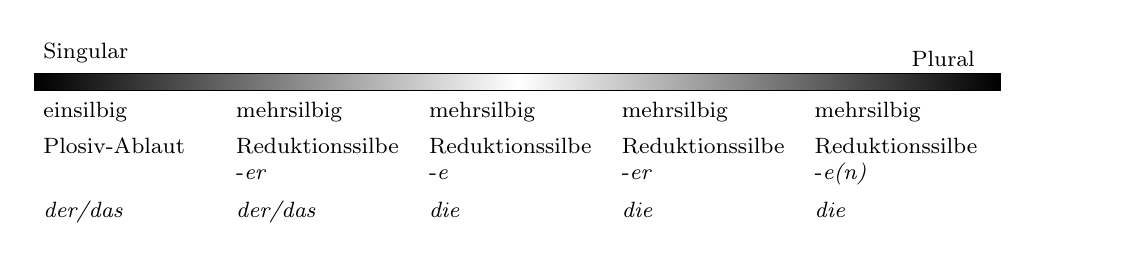
\begin{tikzpicture}\footnotesize
	\matrix (sgpl)
	        [matrix of nodes, 
	         nodes in empty cells,
	         nodes={text width=2.25cm},
	         row 1 column 5/.style={right}]
	  {
	  	Singular & & & &Plural\\
	  	& & & & \\[0.5ex]
	    einsilbig & mehrsilbig & mehrsilbig & mehrsilbig & mehrsilbig\\
	    Plosiv-Ablaut & Reduktionssilbe -\textit{er} & Reduktionssilbe -\textit{e} & Reduktionssilbe -\textit{er} & Reduktionssilbe -\textit{e(n)}\\
	    \textit{der/das} & \textit{der/das} & \textit{die} & \textit{die} & \textit{die}\\
  	  };
    \draw[left color=black,right color=black,middle color=white]
    (sgpl-2-1.north west) rectangle (sgpl-2-5.south east);
\end{tikzpicture}
\caption{Kontinuum der Singular- und Plural-Schemata nach \textcites[332]{Köpcke1988}[88]{Köpcke1993}}
\label{fig:2}
\end{figure}

In \citegen[71]{Köpcke1993} Modell nehmen Schemata eine quasi vermittelnde Stellung zwischen regelbasiertem Item-and-Process-Modell und mor"-pho"-lo"-gi"-schen Modellen ein, die Flexive nicht als unabhängige sprachliche Zeichen, sondern Flexionsformen als Teil der lexikalischen Repräsentation eines Lexems im mentalen Lexikon erfassen. Beide Idealtypen werden nach \citet[98--100]{Köpcke1993} den psycholinguistischen Realitäten der Sprachproduktion und -perzeption nicht gerecht. In IP-Modellen sind Basisformen und Regeln im mentalen Lexikon gespeichert, was bei regulären Pluralformen ökonomisch, bei irregulären, aber hochfrequenten Formen dagegen maximal unökonomisch ist. Modelle, die eine lexikalische Speicherung morphologischer Formen annehmen, sind wiederum bei den hochfrequenten, irregulären (im Extremfall suppletiven) Formen ökonomisch, nicht aber bei regulären Ausdrücken. Schemata operieren „zwischen“ diesen beiden Idealtypen \citep[100]{Köpcke1993}.

Anders als \citeua{Bybee1985b} integriert \citet{Köpcke1993} IP-Regeln und Schemata in sein Grammatikmodell, indem er -- mit Blick auf die Kompetenz der Sprachnutzer -- von einer Koexistenz der analytischen Fähigkeiten ausgeht, die eine Segmentierung komplexer Ausdrücke ermöglichen, und von Kategorisierungen, die „auf holistische Repräsentationen“ von Wörtern und Wortformen im Lexikon „zurückzuführen sind“ \citep[215]{Köpcke1993}. In neueren Arbeiten wird die analytische Kompetenz der Sprachnutzer zudem berücksichtigt, indem sogenannte Schemata zweiter Ordnung (auch Paar-Schemata) angenommen werden (\citealt{Nesset2008}, \citealt{KöpckeEtAl2021}, \citealt{KöpckeWecker2017}, \citealt{Ronneberger-Sibold2021}, \citealt{Wecker2016}). Das heißt, im mentalen Lexikon finden sich nicht nur isolierte Schemata („Schemata erster Ordnung“), z.\,B. das Singular-Schema [die + \#\_\_\_-e], sondern das Plural-Schema [die + \#\_\_\_-en] wird als Schema zweiter Ordnung assoziiert, die paradigmatische Beziehung ist als Teil der mentalen Repräsentation abgespeichert. Anders als das outputbasierte Schema erster Ordnung basiert das Schema zweiter Ordnung auf Generalisierungen von verschiedenen Wortformen und ihren paradigmatischen Beziehungen, es ist also inputbasiert und verbindet -- als eine Art „‚Super‘-Schema“ (\citealt[85]{KöpckeWecker2017}) -- zwei Schemata erster Ordnung miteinander (siehe auch \sectref{sec:10.3.1}).

Dass die Annahme von Schemata und auch die probabilistische Interpretation der perzeptuellen Hinweisreize plausibel sind, zeigen \citet{DomahsEtAl2017} in einer Studie mit einer Patientin mit Progressiver Aphasie, deren lexikalisches Wissen, nicht aber das sprachliche Regelwissen gestört ist. Ausgehend von der Hypothese, dass schemabasiertes Wissen mehr oder weniger unabhängig von lexikalischem Wissen existiert, erweist sich das Leistungsmuster der Patientin bei Numerusentscheidungsaufgaben als „konsistent mit der Annahme einer schemabasierten Antwortstrategie“ (\citealt[227]{DomahsEtAl2017}).\footnote{Zum einen erwiesen sich die Art des Definitartikels, Silbenanzahl sowie das zusätzlich getestete Merkmal eines trochäischen Betonungsmusters als statistisch signifikante Hinweisgeber für eine Pluralentscheidung. Zum anderen konnte keiner dieser Cues isoliert das Antwortverhalten erklären; die Hinweisreize bewirkten in Kombination eine probabilistische Verarbeitung der Numerusinformation (vgl. \citealt[228]{DomahsEtAl2017}).} Bemerkenswert ist hier das Fazit, dass „die besonderen Stärken“ (\citealt[229]{DomahsEtAl2017}) des Schema-Ansatzes eher im Bereich der Perzeption von morphologischen Markierungen gesehen werden, während \citet{Köpcke1988, Köpcke2000b} in Kunstwort-Experimenten stärker die schemabasierte Produktion im Blick hatte. Dass es bei der Produktion Variation sowohl in der horizontalen (arealen) als auch in der vertikalen Dimension gibt, zeigt \citet{Ronneberger-Sibold2021}, die \citegen{Köpcke2000b} Kunstwort-Experiment mit Probanden aus dem bair. Dialektraum wiederholt hat. Im Fokus des \sectref{sec:10.3} steht indes der Aspekt der Perzeption von morphologischen Markierungen: Welche Cues werden von Sprechern genutzt, um die morphologische Information zu kodieren und wie verhalten sich diese Cues mit Blick auf die prototypische Struktur von Schemata? Und welche Hinweisreize sind mehr oder weniger informativ mit Blick auf die morphologische Funktion und wie gut sind sie perzipierbar? Während \citet{Köpcke1993} dies für die standarddeutsche Pluralallomorphie modelliert hat, steht dies für dialektale Flexionssysteme noch aus.

\chapter{Methodisches Vorgehen}\label{chap:6}\largerpage[2]
Hinsichtlich des Umfangs des zu analysierenden Datenmaterials und der Dichte des Ortsnetzes musste zunächst die grundsätzliche Entscheidung zwischen einer quantitativ umfangreichen und einer qualitativ tiefgehenden Untersuchung getroffen werden. Ich habe mich für einen Kompromiss zwischen diesen beiden legitimen Forschungsinteressen entschieden, der eine in meinen Augen aussagekräftige, und zugleich machbare Lösung darstellt. Untersucht wurde das nominale Flexionssystem von 37 Tiefenbohrungspunkten in den oobd. Dialekten Bayerns. Ziel und Anspruch dieses Vorgehens ist es, durch ein Ortsnetz von Tiefenbohrungspunkten, die Nominalflexion in der arealen Dimension darzustellen und zugleich die Flexionssysteme der einzelnen Ortspunkte zu erfassen. Pro Ortspunkt war durch das umfangreiche Fragebuch des \textit{Bayerischen Sprachatlas} (und hierin speziell die Fragen zur Nominalflexion) eine qualitative Auswertung des Datenmaterials möglich. Durch die Dichte des BSA-Ortsnetzes können außerdem die Daten benachbarter Ortspunkte zum Vergleich herangezogen und die Analysen der einzelnen Tiefenbohrungspunkte durch weitere Datenpunkte abgesichert werden. Ergänzt wurde die primäre Materialbasis durch weitere Datenquellen (siehe \sectref{sec:6.2}), sodass für die einzelnen Tiefenbohrungspunkte (wo möglich) eine Kurzeitdiachronie aufgestellt werden konnte. \sectref{sec:6.1} gibt zunächst einen Überblick über die Auswahlkriterien des Untersuchungsgebiets (UG) und der einzelnen Tiefenbohrungspunkte. In \sectref{sec:6.3} wird schließlich die Methodik der Datenaufbereitung und -auswertung dargestellt.

\section{Untersuchungsgebiet und Tiefenbohrungspunkte}
\label{sec:6.1}
Gegenstand der Untersuchung sind die Darstellung und der Vergleich von Flexionssystemen einzelner Ortsdialekte des oobd. Dialektraumes. Wieso ist eine Fokussierung der oobd. Dialekte Bayerns sinnvoll? Zum einen ist dies durch die gute Datensituation für eine dialektvergleichende Untersuchung der Flexionsmorphologie in diesem Gebiet bedingt, zum anderen ergibt sich dies aus der Außenabgrenzung und der inneren Struktur des Dialektraums. So zeigt \citet{Lameli2013} mit einer raumstatistischen Reanalyse von Wredes Dialekteinteilungskarte, dass der oobd. Dialektraum in seiner Außenabgrenzung einen spezifischen, in sich geschlossenen Dialektraum bildet. Die drei Teilräume Ofr., Nord- und Mittelbair. wiederum weisen hinsichtlich ihrer phonologischen Strukturen sowohl Spezifika als auch Gemeinsamkeiten auf, was eine Untersuchung der Numerusflexion eines größeren Dialektraumes unter verschiedenen phonologischen Bedingungen in ihren Ähnlichkeiten und Unterschieden (ganz im Sinne eines Dialektlabors, siehe \chapref{chap:2}) ermöglicht (vgl. \citealt[3]{Rowley1997}).


\begin{map}
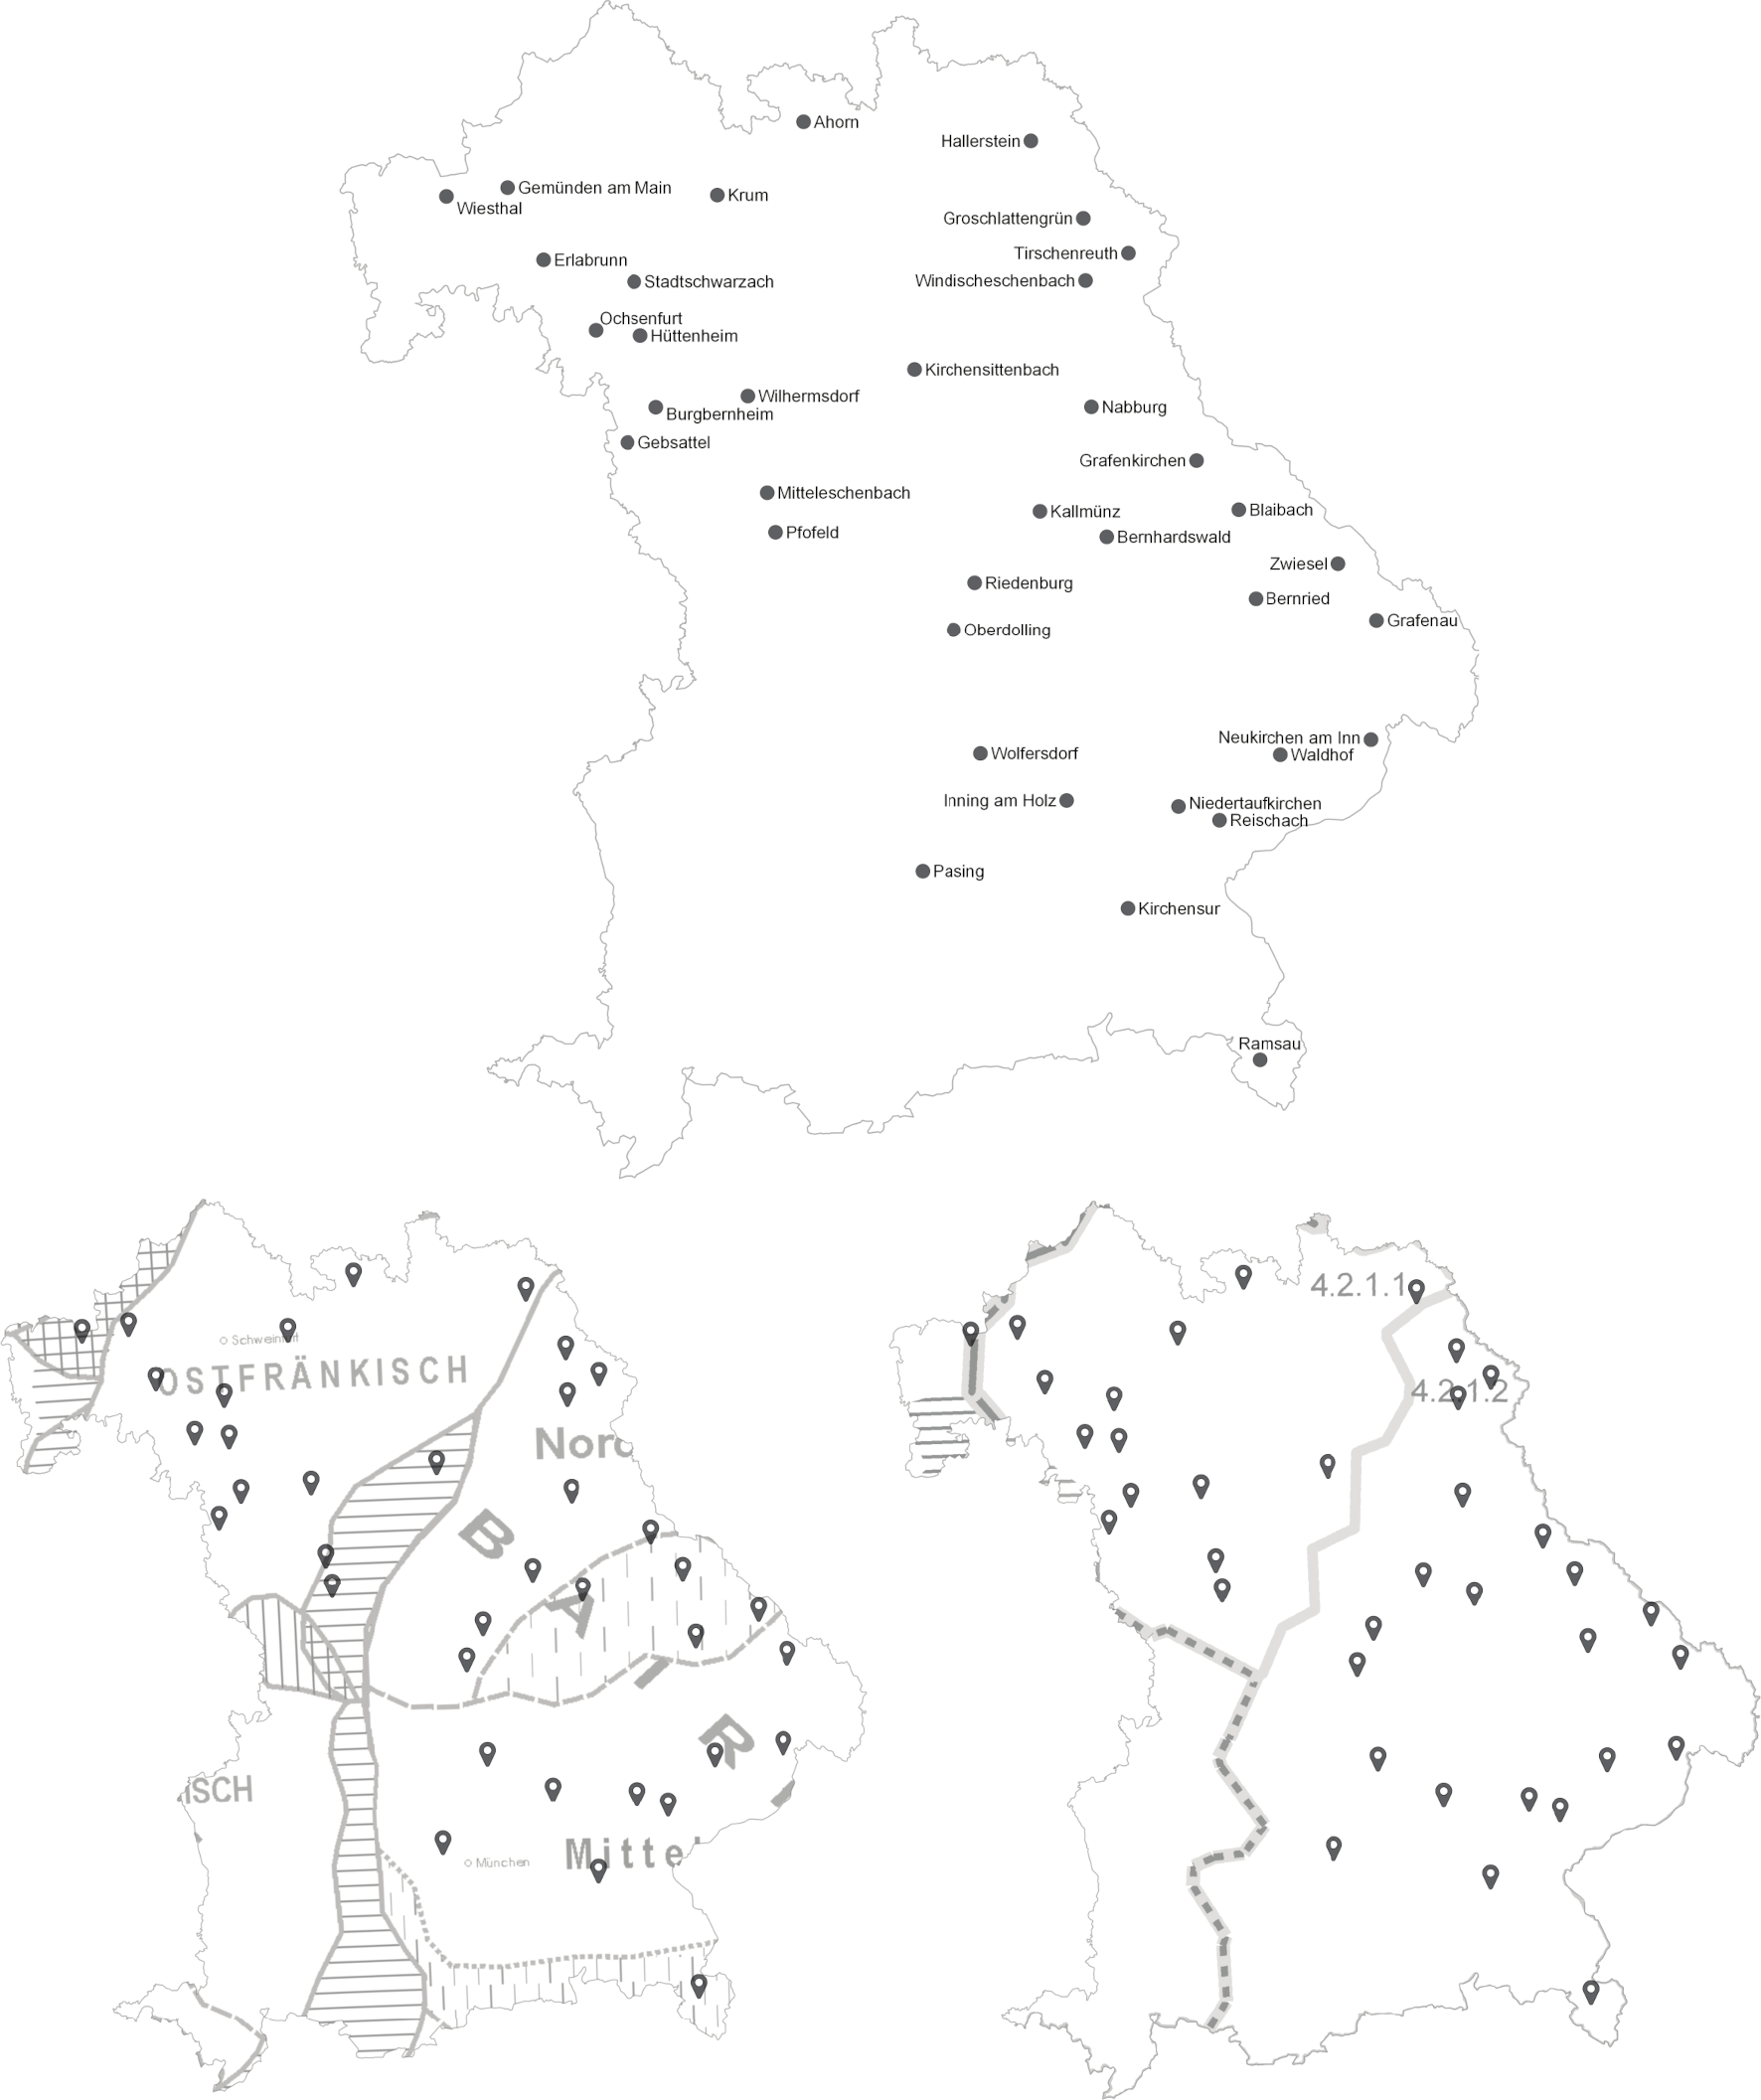
\includegraphics[width=\textwidth]{figures/Karte1.png}
\caption{Tiefenbohrungspunkte sowie Ortspunkte mit den Dialektgliederungen von \citet[Karte 47.4, unten links]{Wiesinger1983b} und \citet[194, unten rechts]{Lameli2013}}
\label{map:1}
\end{map}

Die Abgrenzung des Ofr. und dessen spezifischer Dialektmerkmale wurden in der Literatur unterschiedlich bewertet (vgl. den Überblick in \citealt{Harnisch2019} und \citealt{Rowley1990a}). Anhand einer
Analyse von Similaritätsrelationen von obd. Referenzorten\footnote{Die obd. Referenzorte sind Kitzingen (Ofr.), Dachau (Mittelbair.), Reutlingen (Schwäbisch).} belegt \citet[168ff.]{Lameli2013} zum einen, dass es „eine starke Anbindung“ des Ofr. an das Bair. gibt, „die umgekehrt nicht gleichermaßen vorliegt“. Zum anderen weisen die Ähnlichkeitswerte des Schwäbischen und deren im Vergleich zu den anderen obd. Dialekträumen weniger große Reichweite darauf hin, dass eine Grobunterteilung des Oberdeutschen in West- und Ostoberdeutsch sinnvoll ist.\footnote{Dieser Befund wird gestützt durch die Analyse von Phylogrammclustern, die eine enge Verbindung zwischen dem ofr. und bair. (d.\,h. oobd.) Sprachraum gegenüber einem alem. und schwäb. (westoberdeutschen) Sprachraum visualisieren (\citealt[187f.]{Lameli2013}).} In der Analyse \citegen[169f.]{Lameli2013} zeigt Kitzingen als ofr. Referenzort „eine klar oberdeutsche Prägung“, wenngleich der Similaritätsvergleich auch Ähnlichkeiten zu den mitteldeutschen Dialekten aufzeigt und damit die Stellung des Ofr. zwischen mittel- und oberdeutschem Sprachraum bestätigt. Zugleich bildet das Ähnlichkeitsprofil von Kitzingen eine Binnendifferenzierung des Ostfränkischen in Unter- und Oberofr. durch die sogenannte Steigerwaldschranke ab, wobei das Oberofr. wiederum ein Übergangsgebiet zum Bair. darstellt (\citealt[203, FN 274]{Lameli2013}). Für den bair. Dialektraum stellt \citet[171]{Lameli2013} fest, dass er in seiner räumlichen Ausdehnung das größte und hinsichtlich der Similaritätswerte einheitlichste Areal unter den deutschen Dialekten bildet. Die Similaritätsmuster illustrieren zugleich „nachdrücklich die signifikante Mittelstellung“ des Nordbair. zwischen dem ofr. und bair. UG (\citealt[173]{Lameli2013}, vgl. \citealt[288--290]{Koch2019} und \citealt[171--174]{Rowley1997}).\largerpage[2]

Eines der Untersuchungsziele besteht in der Beschreibung der horizontalen Variationsdimension der Pluralmarkierung: Sind bestimmte Pluralkodierungsverfahren dialekt(raum)spezifisch und arealbildend? Daneben soll untersucht werden, ob und inwiefern phonologische Voraussetzungen die Flexionsmorphologie bedingen, also in welchem Maße das Pluralmarkerinventar durch das Phoneminventar und/oder durch phonologische Prozesse gesteuert ist. Die Auswahl der Tiefenbohrungspunkte musste daher einem doppelten Kriterium entsprechen. Zum einen sollen sie die verschiedenen Dialekträume im UG abbilden, zum anderen sollen die phonologischen Voraussetzungen so variant sein, dass sie einen Vergleich von dialektalen Markierungsstrategien und phonologischen Variablen ermöglichen. Ausgewählt wurden Ortspunkte, für die in jedem Falle ein Wenker-Bogen und nach Möglichkeit auch eine Orts- oder Landschaftsgrammatik vorliegt, sodass nicht nur der synchrone Formenbestand der Pluralmarker, sondern auch eine Kurzzeitdiachronie untersucht werden konnte. Um sicherzustellen, dass eine mögliche Raumbildung nicht durch zufällige Unterschiede im erfassten Datenmaterial, sondern aus einer inhärenten Systematik abzuleiten ist, wurden immer mehrere, räumlich nahe Ortspunkte definiert („Cluster“). Idealerweise sollten sowohl vor dem Hintergrund einzelner Arbeitsgebiete der BSA-Teilprojekte als auch für die einzelnen Dialekträume im UG eine ausgeglichene Menge solcher Tiefenbohrungspunkte definiert werden.

Für die Auswahl der Ortspunkte ermöglichten vorhandene Dialekteinteilungen (\citealt{Wiesinger1983b}, \citealt{Lameli2013}) einen ersten Zugang. Methodisch besteht dabei die Gefahr eines Zirkelschlusses, da Dialekteinteilungen primär auf phonologischen neben morphologischen Varianten basieren und die ausgewählten Tiefenbohrungspunkte diese Befunde im schlimmsten Fall nur reproduzieren. Dies kann insofern relativiert werden, als jede Dialekteinteilung das Ergebnis einer qualitativen Kontrastierung bestimmter Kriterien (d.\,h. prototypischer Varianten) und damit das Ergebnis einer Reduzierung der arealtypologischen Komplexität der sprachlichen Wirklichkeit ist \citep[8]{Lameli2013}. So basiert die strukturelle Dialekteinteilung \citegen{Wiesinger1983b} vor allem auf prototypischen phonologischen neben (flexions-)morphologischen Kriterien, die als Einzelvarianten und in Form einer Zusammenfassung zu Variantenbündeln die Grundlage dieser Dialektklassifikation sind \citep[812--814]{Wiesinger1983b}. Eine tiefergehende Analyse der nominalen Flexionsformen geht weit über diese ausgewählten Varianten hinaus und ergänzt diese vielmehr, als dass sie nur reproduziert werden.\largerpage

Ein Spezifikum und großer Vorteil der Wiesinger-Einteilung ist die Unterscheidung von Kern- und Übergangsgebieten, die aus der Einteilungskarte hervorgeht (\citealt[830f. und Karte 47.4]{Wiesinger1983b}; vgl. \citealt[188--189]{Lameli2019}). In der vorliegenden Untersuchung wurden neben den Kern- auch Übergangs- und Randgebiete berücksichtigt: Unterostfränkisch (inklusive ofr.-hess. Übergangsgebiet), Oberostfränkisch, nördliches Nordbairisch (inklusive ofr.-nordbair. Über"-gangs"-ge"-biet), südliches Nordbairisch und nordbair.-mittelbair. Übergangsgebiet, Mittelbair. (inklusive mittelbair.-südbair. Übergangsgebiet). Aus dem Pool möglicher Tiefenbohrungspunkte (d.\,h. Ortspunkten, die sowohl Wenker- als auch BSA-Erhebungsorte waren) wurden in einem nächsten Schritt Ortspunkte mit möglichst differenten phonologischen Profilen gewählt. Hierfür wurden die Karten des \textit{Deutschen Sprachatlas} („Wenker-Atlas“, \citealt{WA}), die publizierten BSA-Bände sowie Dialektgrammatiken und -darstellungen hinsichtlich verschiedener phonologischer Prozesse gesichtet (\tabref{tab:12}). Neben diesen phonologischen Variablen bildeten potenzielle Unterschiede der Numerusmorphologie im intervarietären Vergleich oder im Vergleich von Standard und Dialekt ein weiteres Auswahlkriterium.


\mapref{map:1} zeigt die 37 definierten Tiefenbohrungspunkte. Für den Westen des Ofr. und auch für die nordbair. Cluster wurde jeweils ein dichteres Ortsnetz gewählt, da hier Isoglossen verschiedener Variablen des Vokalismus und der Reduktionssilbe verlaufen (vgl. \citealt[399]{Rowley1990a}). Die Durchsicht vorhandener Sprachkarten zu den einzelnen Phänomenen bestätigt dagegen \citegen[171]{Lameli2013} Befund, dass das Mittelbair. innerhalb des bair. Dialektraum ein sprachlich konsistentes Gebiet bildet, weswegen hier ein weniger dichtes Ortsnetz definiert wurde.\largerpage

\begin{table}
\caption{Phonologische und flexionsmorphologische Kriterien sowie Binnengliederung des UGs (vgl. \citealt[4--5]{Rowley1997})\label{tab:12}}

\begin{subtable}{\textwidth}
\caption{Vokalqualität I\label{tab:12a}}
\small
\begin{tabularx}{\textwidth}{>{\raggedright\arraybackslash}p{.2\textwidth}QQ}
\lsptoprule

\multicolumn{2}{p{.45\textwidth}}{Auswahlkriterien der (historischen) Phonologie und Flexions\-morphologie} & Binnengliederung des Untersuchungs\-gebiets: Dialektraum und Ortsdialekte\\
\midrule
Umlaut\slash Nicht-Eintreten des Umlauts & Umlaut/Nicht-Umlaut bei mhd. \textit{u}/\textit{ü} (vgl. \citealt{Hinderling2004}, \citealt[159ff.]{SNOB1}) & Bair. Cluster, nordöstliches Ofr. (Ahorn, Hallerstein)\\
\tablevspace
Hebung\slash Senkung & Hebung und z.\,T. Diphthongierung von mhd. \textit{e}, \textit{ö}, \textit{o} in Dehnung (\citealt{Gütter1971}: Karte 3/4, \citealt{Rowley1997}: 73--74/Karte 15) & nördliches Nordbair. (Gro\-schlat\-ten\-grün, Windischeschenbach, Tir\-schen\-reuth) und Coburger, Nürnberger und Weißenburger Raum (Ahorn, Kirchensittenbach, Mittelschenbach, Pfofeld)\\
\tablevspace
& Senkung von mhd. \textit{i} & Wiesthal\\
\tablevspace
& Senkung\slash Zentralisierung von mhd. \textit{ë} (\citealt{WA}-Karten 405 „Berge“, 524 „Felde“) & Hüttenheim, Stadtschwarzach\\
\tablevspace
Rundung\slash Entrundung & Rundung von Palatalvokalen (vgl. \citealt[1103]{Wiesinger1983e}, \citealt{WA}-Karte 465 „Häuser“) & ofr.-hess.-hennebergisches Gebiet (unterofr. Cluster, ofr. Ahorn)\\
\tablevspace
& Entrundung von Palatalvokalen (\citealt{WA}-Karte 465 „Häuser“) & Nürnberger Raum, Nord- und Mittelbair.\\
\lspbottomrule
\end{tabularx}
\end{subtable}
\end{table}


\begin{table}
\ContinuedFloat
\caption{Phonologische und flexionsmorphologische Kriterien sowie Binnengliederung des UGs (vgl. \citealt[4--5]{Rowley1997})}

\begin{subtable}{\textwidth}
\caption{Vokalqualität II}
\label{tab:12b}
\small
\begin{tabularx}{\textwidth}{>{\raggedright\arraybackslash}p{.25\textwidth}QQ}
\lsptoprule

\multicolumn{2}{p{.45\textwidth}}{Auswahlkriterien der (historischen) Phonologie und Flexions\-morphologie} & Binnengliederung des Untersuchungs\-gebiets: Dialektraum und Ortsdialekte\\
\midrule
Monophthongierung/ Diphthongier\-ung & Monophthongierung der Diphthongierungsprodukte bei mhd. \textit{î}, \textit{û}, \textit{iu} (sogenannte „tertiäre Monophthonge“, vgl. \citealt{Wildfeuer2004}, \citealt{WA}-Karten 51 „Eis“, 373 „Hause“, 465 „Häuser“) & südöstliches Nordbair., nordbair-mittelbair. Übergangsgebiet (Bernried, Blaibach, Grafenkirchen)\\
\tablevspace
& Monophthongierung von mhd. \textit{öu} (vgl. \citealt{WA}-Karte 380 „Apfelbäumchen“) & ofr. und mittelbair. Cluster \\
\tablevspace
& Monophthongierung von mhd. \textit{ei} (vgl. \citealt{WA}-Karten 96 „Eier“, 443 „Seife“) & Ofr., bei \textit{Ei} nur im unterofr. Cluster (Erlabrunn, Gemünden, Hüttenheim, Ochsenfurt, Wiesthal)\\
\tablevspace
& Vokalwechsel von mhd. \textit{ei} in historischen Ein- und Mehrsilbern & Nordbair. und nordbair.-mittelbair. Über\-gangsgebiet, nordöstl. Mittelbair.\\
\lspbottomrule
\end{tabularx}
\end{subtable}
\end{table}


\begin{table}
\ContinuedFloat
\caption{Phonologische und flexionsmorphologische Kriterien sowie Binnengliederung des UGs (vgl. \citealt[4--5]{Rowley1997})}

\begin{subtable}{\textwidth}
\caption{Konsonantismus}
\label{tab:12c}
\small
\begin{tabularx}{\textwidth}{>{\raggedright\arraybackslash}p{.25\textwidth}QQ}
\lsptoprule

\multicolumn{2}{p{.45\textwidth}}{Auswahlkriterien der (historischen) Phonologie und Flexions\-morphologie} & Binnengliederung des Untersuchungs\-gebiets: Dialektraum und Ortsdialekte\\
\midrule
Fortis-Lenis-Opposition & Aufhebung der Fortis/Lenis-Opposition in allen Positionen & Ofr.\\
\tablevspace
& „Bair. Silbengesetz“ & Nord- und Mittelbair.\\
\tablevspace
Liquidvokalisierung & Vokalisierung von /l/ zu [i] (\citealt{Gütter1971}: Karte 6) & mittelbair. Cluster, nordbair.-mittelbair. Übergangsgebiet\\
\lspbottomrule
\end{tabularx}
\end{subtable}
\end{table}

\begin{table}
\ContinuedFloat
\caption{Phonologische und flexionsmorphologische Kriterien sowie Binnengliederung des UGs (vgl. \citealt[4--5]{Rowley1997})}

\begin{subtable}{\textwidth}
\caption{Reduktionssilben}
\label{tab:12d}
\small
\begin{tabularx}{\textwidth}{>{\raggedright\arraybackslash}p{.2\textwidth}QQ}
\lsptoprule

\multicolumn{2}{p{.45\textwidth}}{Auswahlkriterien der (historischen) Phonologie und Flexions\-morphologie} & Binnengliederung des Untersuchungs\-gebiets: Dialektraum und Ortsdialekte\\
\midrule
Schwa-Erhalt\slash Apokope & Schwa-Erhalt bei \textit{Gänse}, \textit{Berge} (\citealt{WA}-Karten 188, 406) & Hallerstein, Pfofeld, Wiesthal\\
\tablevspace
vokalische Realisierung des Nasalsuffixes & Vokalische Realisierung des Nasalsuffixes in allen Positionen und phonologischen Umgebungen (\citealt{WA}-Karten 444 „Seife“, 492 „Bauern“, 495 „Ochsen“, 546 „hinten“) & „Vokalisierungsstreifen“ im westlichen Ofr. (Erlabrunn, Gebsattel, Gemünden, Ochsenfurt)\\
\tablevspace
& Vokalisierung des Nasalsuffixes in Abhängigkeit von der phonologischen Umgebung & mittleres und östl. Ofr., Nord- und Mittelbair. \\
\lspbottomrule
\end{tabularx}
\end{subtable}
\end{table}

\begin{table}
\ContinuedFloat
\caption{Phonologische und flexionsmorphologische Kriterien sowie Binnengliederung des UGs (vgl. \citealt[4--5]{Rowley1997})}

\begin{subtable}{\textwidth}
\caption{Nominale Flexionsmorphologie}
\label{tab:12e}
\small
\begin{tabularx}{\textwidth}{>{\raggedright\arraybackslash}p{.2\textwidth}QQ}
\lsptoprule

\multicolumn{2}{p{.45\textwidth}}{Auswahlkriterien der (historischen) Phonologie und Flexions\-morphologie} & Binnengliederung des Untersuchungs\-gebiets: Dialektraum und Ortsdialekte\\
\midrule
einzelne Phänomene der Formenbildung & subtraktive Pluralmarkierung (vgl. \citealt{Köhler1934}) & Gemünden am Main, Wiesthal\\
\tablevspace
& keine Pluralmarkierung durch Quantitätskontraste (\citealt{SMF7}: Karte 21) & Wilhermsdorf\\
\tablevspace
& schwache Pluralmarkierung bei \textit{Berge} (\citealt{WA}-Karte 406) & Bernried, Blaibach, Waldhof\\
\tablevspace
& Singularstammbildung der historisch schwachen Feminina: keine \textit{n}{}-Erweiterung, sondern Apokope (\citealt{WA}-Karte 444 „Seife“) & südbair.-mittelbair. Übergangsgebiet (Ramsau bei Berchtesgaden)\\
\tablevspace
& erweitertes Nasalsuffix im Dativ Plural (\citealt{SMF7}: Karte 24) & Mitteleschenbach\\
\tablevspace
& kein Nasalsuffix im Dativ Plural (\citealt{SMF7}: Karte 24) & westliches Ofr. (Burgbernheim, Gebsattel)\\
\lspbottomrule
\end{tabularx}
\end{subtable}
\end{table}

\clearpage
\section{Die Materialbasis}\label{sec:6.2}
\begin{sloppypar}
Die Datenbasis besteht aus drei verschiedenen Quellentypen: als primäre Datenbasis die Erhebungsdaten des \textit{Bayerischen Sprachatlas} und die Sprachatlanten der einzelnen Teilprojekte (\sectref{sec:6.2.1}), daneben die Daten der Wenker-Erhebungen und die Karten des \textit{Sprachatlas des Deutschen Reiches} (\sectref{sec:6.2.2}) und diverse grammatische Beschreibungen der untersuchten Dialekte (insbesondere Orts- und Landschaftsmonografien, aber auch Zeitschriftenbeiträge oder nicht publizierte Qualifikationsarbeiten, vgl. \sectref{sec:6.2.3}). Die Datenbasis ist damit ausgesprochen heterogen in ihrer methodischen Ausrichtung und Darstellung, bezieht sich aber jeweils auf den Basisdialekt als am weitesten vom Standard entfernte Varietät.
\end{sloppypar}

Indem die vorliegende Arbeit das vorhandene Erhebungsmaterial des \textit{Bayerischen Sprachatlas} und historisches Datenmaterial aus Orts- und Landschaftsgrammatiken verwendet, ist sie an die abgefragten bzw. behandelten, meist isolierten Flexionsformen dieser Quellen und an einen sehr spezifischen Ausschnitt meist landwirtschaftlicher Lexik gebunden. Jüngere Arbeiten haben indes gezeigt, dass die Auswertung von Dialektgrammatiken als Datenquellen für morphologische Fragestellungen ein sinnvolles und gewinnbringendes Unterfangen darstellt (vgl. \citealt{Birkenes2014, Fischer2018, Fischer2019}). Gleichzeitig ist es durch die digitale Verfügbarkeit beinahe des gesamten Abfragematerials der Teilprojekte des \textit{Bayerischen Sprachatlas} und der Wenker-Materialien möglich, Datenmaterial und Karten zu den einzelnen Teilsystemen der Grammatik für die Tiefenbohrungspunkte oder ganze Dialekträume zu vergleichen und systematisch in die Datenauswertung einzubeziehen.

Eine methodische Schwierigkeit bei der Nutzung vorhandener Dialektdaten zu einer flexionsmorphologischen Fragestellung besteht nach wie vor darin, dass in dem zur Verfügung stehenden Datenmaterial kaum vollständige Flexionsparadigmen belegt sind, während für den Bereich der Phonologie -- dies entspricht dem primären Erkenntnisinteresse der traditionellen Dialektologie -- das gesamte phonologische System ausgehend vom mhd. Protosystem erhoben wurde. In der Nominalflexion wurden meist nur einzelne Paradigmenstellen abgefragt, im Falle des BSA beispielsweise Nominativ Singular und Plural, z.\,T. Akkusativ \mbox{und}\slash oder Dativ Singular und\slash oder Plural (vgl. \citealt[814]{Rabanus2010}). Der Vorteil der Daten des \textit{Bayerischen Sprachatlas} besteht in erster Linie darin, dass für das gesamte Untersuchungsgebiet ein weitgehend einheitliches Fragebuch verwendet wurde. Für Einzellexeme ist die Datenlage damit vergleichsweise gut; Nominalphrasen wurden noch selektiver erhoben und z.\,T. nicht vollständig transkribiert, weswegen sie im Rahmen der Untersuchung nur für die syntaktische Einheit Definitartikel und Substantiv systematisch aufbereitet wurden.

Tonkorpora (zum Beispiel das Zwirner-Korpus im \textit{Archiv für Gesprochenes Deutsch} oder die Tonaufnahmen der BSA-Teilprojekte, die bei den Explorationen aufgenommen wurden) wurden in dieser Untersuchung nicht berücksichtigt. Spontansprachliches Material ist für eine flexionsmorphologische Untersuchung zwar wünschenswert (v.\,a. dann, wenn Synkretismen vorliegen und die Sprecher Ambiguitäten auflösen müssen) und auch reich an flexivischen Formen, jedoch ist die Auswertung ausgesprochen aufwendig und bei freien Dialogen eine entsprechend große Menge an Datenmaterial nötig, wenn ein ähnlich vergleichbares Korpus aufgebaut werden soll, wie es dieser Arbeit zugrunde liegt (vgl. hierzu auch \citealt[37]{Birkenes2014}, \citealt[39]{SchmidtEtAl2019}).

\subsection{Der \textit{Bayerische Sprachatlas} und seine Teilprojekte}
\label{sec:6.2.1}

\begin{quote}
Wir sehen die Fertigstellung der Bände nicht als das Ende, sondern als den entscheidenden Schritt für die weitere dialektologische Arbeit an. \\\hbox{}\hfill\hbox{(\citealt[7]{SNiB3})\footnote{Die Kurzzitation der publizierten Bände des \textit{Bayerischen Sprachatlas} nennt jeweils Teilprojekt und Bandnummer (z~B. SNiB 3 für \textit{Sprachatlas von Niederbayern}, Band 3), eine Aufschlüsselung der zitierten Bände findet sich im Literaturverzeichnis.}}
\end{quote}

Der \textit{Bayerische Sprachatlas} steht in der Tradition von Georg Wenkers \textit{Sprachatlas des Deutschen Reichs}, setzt zugleich die Methodik des \textit{Sprachatlas der Deutschen Schweiz} von Rudolf Hotzenköcherle fort und knüpft damit an die Methodik der Sprachatlanten der sogenannten zweiten Generation: die direkte Befragung der ältesten ortsansässigen Informanten (\textit{non-mobile, old, rural males} und \textit{females}, vgl. \citealt[29]{ChambersTrudgill2009}) durch geschulte Exploratoren, um so einzig die horizontale, d.\,h. diatopische Dimension von Variation zu erheben. Ziel der direkten Erhebungen im Rahmen der BSA-Teilprojekte war es, „den jeweils ältesten noch erreichbaren Sprachstand zu Papier zu bringen“ (\citealt[25]{SBS1}). Die Einzelinformation der befragten NORMs und NORFs und ihre metasprachliche Kompetenz stehen damit repräsentativ für den jeweiligen Ortsdialekt (vgl. \citealt[500--501]{König2010}). Als Ergebnis dieser Operationalisierung der repräsentativen Einzelinformation durch NORMs/NORFs arbeitet die traditionelle Dialektologie mit einer sehr spezifischen Form von Sprachdaten: Die erhobene Varietät, der Basisdialekt (auch Grunddialekt), ist, wie \citet[24f.]{Auer2010} betont, kein der Forschung „vorgängiges und von ihr unabhängiges Objekt der sprachlichen Wirklichkeit“, sondern „ein dem Alltag fremdes, in der Situation der Erhebung entstehendes Objekt“.\footnote{Auch während der BSA-Erhebungen war man sich darüber „bewußt, daß die Auskünfte der Gewährsleute über ihre Sprachverwendung nicht in jedem Fall mit einer aufgrund von Langzeitbeobachtung gewonnen Ortsnorm übereinstimmen müssen“ (\citealt[26]{SBS1}).} Das Datenmaterial der traditionellen Dialektologie ist folglich Ergebnis eines „Konstitutionsprozesses“ \citep{Auer2010}. Der erhobene (intendierte) Basisdialekt muss als Konstrukt zur Datenerhebung verstanden werden (vgl. \citealt[502]{König2010}): „Der Explorator verwandelt die Antworten der Gewährspersonen also in Daten; das Konstrukt Grunddialekt wird durch ihn genauso geformt wie durch den Informanten“ \citep[34]{Auer2010}. Durch das Forschungsziel und das methodische Vorgehen der BSA-Projekte ergibt sich für die entstandenen Sprachatlanten „eine Position zwischen historischer und rezenter Sprachwissenschaft“ (\citealt[37]{SMF1}), das Ergebnis ist die Dokumentation einer Sprachschicht, „die einerseits bereits historisch ist, andererseits aber noch direkt erhoben werden kann“ (ebd.).

Die Arbeitsgebiete der Regionalprojekte des \textit{Bayerischen Sprachatlas} -- mit Ausnahme des \textit{Sprachatlas von Bayerisch Schwaben}, dessen Arbeitsgebiet das gesamte Areal des Alemannischen und Schwäbischen in Bayern abdeckt -- entsprechen den Regierungsbezirken Bayerns (\tabref{tab:13}). Um die jeweilige Größe des Erhebungsgebietes abschätzen zu können, wurden als Referenz die Anzahl der Planquadrate angegeben (mit einer Kantenlänge von 7 km, geplant war eine Ortsaufnahme pro Planquadrat, vgl. \citealt[21]{Klepsch2013}).

\begin{table}
\begin{tabularx}{\textwidth}{QQll}
\lsptoprule
Teilprojekt & Untersuchungsgebiet & \makecell[tl]{Plan-\\quadrate} & \makecell[tl]{Erhebungs-\\zeitraum}\\
\midrule
Sprachatlas von Mittelfranken

(SMF) & Regierungsbezirk

Mittelfranken & 155 & 1991--1998\\
\tablevspace
Sprachatlas von Unterfranken

(SUF) & Regierungsbezirk

Unterfranken & 180 & 1991--1996\\
\tablevspace
Sprachatlas von Nordostbayern

(SNOB) & Regierungsbezirke

Oberfranken und Oberpfalz & 360 & 1981--1999\\
\tablevspace
Sprachatlas von Niederbayern

(SNiB) & Regierungsbezirk

Niederbayern & 240 & 1991--1998\\
\tablevspace
Sprachatlas von Oberbayern

(SOB) & Regierungsbezirk Oberbayern & 320 & 1991--1998\\
\lspbottomrule
\end{tabularx}
\caption{Die in der Untersuchung berücksichtigten Teilprojekte des \textit{Bayerischen Sprachatlas}}
\label{tab:13}
\end{table}

Die einzelnen Teilprojekte arbeiten mit einem gemeinsamen Fragebuch von rund 2.800 Fragen. Um die Vergleichbarkeit der Teilprojekte zu gewähren, wurde der Aufbau des Fragebuchs nicht verändert, aber um mögliche regionalspezifische Aspekte ergänzt (z.\,B. zum Hopfen- und Weinanbau, mit einem Anteil von bis zu 10\,\% projektspezifischer Fragen am Fragebuch insgesamt, vgl. \citealt[6]{Munske2015}). Die Fragebücher waren nach außersprachlichen Themenbereichen („Das Vieh und seine Pflege“, „Ackerbau“, „Boden und Flur“ etc.) gegliedert und subsumierten darunter sowohl Fragen zur spezifischen Lexik als auch zu sprachstrukturellen Aspekten. Die Exploratorinnen und Exploratoren arbeiteten den vorgedruckten Fragekatalog mit den Gewährspersonen durch, wobei das Gespräch möglichst frei gestaltet sein sollte (vgl. \citealt[31]{SMF1}). Ziel der semasiologischen Fragestellungen im Fragebuch war es, „Aufschluß über die Strukturen der Mundart“ zu erhalten und schließlich mithilfe des dokumentierten Sprachmaterials jeder Ortsaufnahme eine Ortsgrammatik anfertigen zu können (\citealt[31]{SMF1}).


\begin{table}
\small
\begin{tabularx}{\textwidth}{lQcccccccc}
\lsptoprule

& Band & Genus & \multicolumn{2}{c}{ Flexion} & \multicolumn{2}{c}{Nominalphrase} & \multicolumn{3}{c}{ Wortbildung}\\
\cmidrule(lr){4-5}\cmidrule(lr){6-7}\cmidrule(lr){8-10}
&  &  & Num. & Kas. & Art.\slash Pron. & Adj. & Der. & Dim. & Mov.\\
\midrule
SBS & 9.1, 9.2 &  & x & x & x & x & x & x & x\\
SMF & 7 &  & x & x &  &  & x & x & x\\
SUF & 3 &  & x & x & x & x &  & x & x\\
SNiB & 7 & x & x &  &  &  &  & x & \\
SOB & 3 & x & x &  & x &  &  & x & \\
SNOB & \multicolumn{9}{l}{ noch nicht erschienen}\\
\lspbottomrule
\end{tabularx}
\caption{Überblick der behandelten Themen zur Nominalmorphologie in den BSA-Teilbänden (vgl. \citealt[8--9]{Munske2015}). Wortbildungen: „Der.“: Deri\-va\-tion, „Dim.“: Dimi\-nu\-tion, „Mov.“: Mo\-vie\-rung}
\label{tab:14}
\end{table}

Diesem Forschungsziel entsprechend bilden die BSA-Fragebücher und im Ergebnis die publizierten Bände alle Sprachebenen ab (zum Teil mit regionalen Schwerpunkten wie dem Syntax-Programm des SNiB). Doch auch in den Teilprojekten des \textit{Bayerischen Sprachatlas} (wie auch in anderen Sprachatlasprojekten) bildete die Phonologie (neben der Lexik) den zentralen Interessensbereich, was sich bereits im Fragebuch, vor allem aber an Umfang und Anzahl der publizierten Bände ablesen lässt. Die Phonologie ist auf mehrere Bände getrennt nach Lang- und Kurzvokalismus sowie Konsonantismus aufgeteilt, während die Morphologie zumeist einen Band, z.\,T. aber auch nur einen Halbband umfasst (nur im Fall des SUF und des SBS sind es zwei). Und auch ein Blick in die Inhaltsverzeichnisse der jeweiligen Morphologie(teil)bände zeigt, dass das Ziel respektive Arbeitsprinzip der BSA-Teilprojekte, nämlich die Abbildung der „sprachgeographisch relevanten, d.h. raumbildenden Erscheinungen“ \citep[5]{Munske2015}, dazu führte, dass die (nominale) Flexionsmorphologie als Flexions\textit{system} nur punktuell behandelt wurde. Kartiert wurden v.\,a. Flexionsformen einzelner Lexeme (nach Genus und Pluralmarkierungsverfahren sortiert, daneben ausgewählte Aspekte der Flexion der Substantivbegleiter und der Wortbildung). Da die Auswahl und die Art der Darstellung den jeweiligen Teilprojekten oblagen, sind für das gesamte Untersuchungsgebiet trotz des weitestgehend einheitlichen Fragebuchs nicht dieselben und vor allem nicht sämtliche Lexeme und Phänomenbereiche der Nominalflexion kartiert. Eine flächendeckende Auswertung des gesamten Rohmaterials ist -- dies illustriert \tabref{tab:14} -- auch nach Erscheinen der Bände des \textit{Bayerischen Sprachatlas} ein Desiderat.

Für die vorliegende Untersuchung wurden die nicht-typisierten Rohdaten der BSA-Teilprojekte zur Flexion des Substantivs aufbereitet und ausgewertet (siehe Anhang). Diese sind über die \textit{Bayerische Dialektdatenbank} \textit{BayDat} in einer online verfügbaren Datenbank zugänglich (vgl. \sectref{sec:6.3.1.1}). Eine Untersuchung zur Nominalflexion kann dabei eine andere Zielsetzung und Vorgehensweise verfolgen als ein Sprachatlas: Während es hier vor allem um die Erfassung des Systems geht, bestand das Ziel da eher in der Dokumentation ausgewählter Varianten. Dabei sind die nicht-typisierten Rohdaten ausgesprochen geeignet, um sprachliche Strukturen zu untersuchen und so „den bisherigen sprachgeographischen Schwerpunkt zugunsten eines sprachsystematischen zu verschieben“ (\citealt[22]{Munske2015}, vgl. \citealt[70]{Kretzschmar2018}). So werden -- anders als in einzelnen Morphologiebänden des BSA -- phonetisch-phonologische Varianten weniger stark in den Vordergrund gestellt, die Daten noch stärker abstrahiert und nach einzelnen Konditionierungsfaktoren der Pluralallomorphie und Deklinationsklassenzusammensetzung untersucht. Zugleich kann eine Analyse der Flexion eines Ortsdialekts kaum losgelöst vom grammatischen Gesamtsystem erfolgen (vgl. \citealt[36]{Schmuck2014}). Die publizierten BSA-Bände (insbesondere jene zur Phonologie und zur Syntax), ihre Analysen und Typisierungen dienen im Folgenden daher als zusätzliche Referenz.

Im Rahmen der Untersuchung wurden die transkribierten Belege der direkten Befragungen der Gewährspersonen ausgewertet, d.\,h. Flexionsformen (Substantive, Nominalphrasen sowie vereinzelte Sätze), die von den Gewährspersonen innerhalb einer spezifischen Erhebungssituation realisiert wurden. Abgefragt wurden isolierte Flexionsformen, syntaktische Strukturen und Verwendungskontexte, die durch die Exploratoren vorgegeben und von den Gewährspersonen in den Ortsdialekt übersetzt wurden (vgl. \citealt[23]{Klepsch2013}).\footnote{Im \textit{Sprachatlas von Mittelfranken} (als exemplarisches Beispiel für die BSA-Fragebücher insgesamt) behandeln von den insgesamt 2.541 semasiologischen Fragen des SMF-Fragebuchs die meisten die Grundform, im nominalen Bereich also den Nom.Sg. (vgl. \citealt[24]{Klepsch2013}). Neben der Singularform wurden aus dem Substantivparadigma i.\,d.\,R. auch die Pluralform (278 Fragen) und zum Teil exemplarisch auch oblique Kasusformen (93 Fragen) abgefragt (\citealt[32]{SMF1}). Fragen zur Flexion der Nominalphrase schlüsseln sich für den SMF wie folgt auf: flektierte Formen von Adjektiven (121 Fragen), Formen von Artikeln (101 Fragen) und Pronomina (293 Fragen).} Da es sich i.\,d.\,R. nicht um spontansprachliches Material, sondern um elizitierte Formen handelt, gilt es aber, die methodischen Spezifika und die Erhebungssituation bei der Auswertung des Datenmaterials zu berücksichtigen (vgl. \citealt{NickelKürschner2019}).

\subsection{\textit{Sprachatlas des deutschen Reichs} und Wenkersätze}
\label{sec:6.2.2}
Die Materialien der indirekten Fragebogenerhebungen, die Georg Wenker im gesamten deutschen Sprachgebiet unternommen hat (1879/80 in Nord- und Mitteldeutschland, 1887/88 in Süddeutschland), und die handgezeichneten Karten des \textit{Sprachatlas des deutschen Reichs} bilden das Vergleichsmaterial, das neben dem \textit{Bayerischen Sprachatlas} als weitere Quelle herangezogen wurde. Wenker-Fragebogen und -Karten sind über die Online-Plattform \textit{regionalsprache.de} (REDE) digitalisiert verfügbar (\citealt{SchmidtEtAl2008ff}).

Es wurden für alle Tiefenbohrungspunkte die für die flexionsmorphologische Analyse relevanten dialektalen Übersetzungen der sog. Wenkersätze ausgewertet. Zwar sind die Wenker-Materialien reich an nominalen Flexionsformen, doch liegen auch hier nur einzelne Paradigmenstellen vor (siehe Anhang für eine Lis\-te der ausgewerteten Items). Außerdem wurden die Wenker-Karten als zusätzliche Referenz zur großräumigen arealen Verteilung von Varianten sowohl für die Vorauswahl der Tiefenbohrungspunkte als auch für Verbreitungsgebiete einzelner phonologischer Prozesse (wie Apokope oder Nasal- und Liquidvokalisierung) herangezogen.

\subsection{Dialektgrammatiken}\label{sec:6.2.3}\largerpage
\begin{sloppypar}
Eine weitere Datenbasis für den empirischen Teil bieten neben den BSA- und Wenker-Materialien dialektologisch-grammatische Darstellungen. Hierzu zählen in erster Linie Orts- und Landschaftsgrammatiken, die das Lautsystem und zum Teil auch die (Flexions-)Morphologie in junggrammatischer Tradition abhandeln (vgl. den Überblick bei \citealt[80--82]{Murray2010}). Daneben gibt es jüngere strukturalistische Untersuchungen, die zumeist das phonologische, teilweise auch das flexionsmorphologische System eines Ortsdialekts behandeln (exemplarisch sind hier für das UG etwa \citealt{Dozauer1967} oder \citealt{Kufner1961} zu nennen). In der Darstellung unterscheiden sich der junggrammatische und der strukturalistische Ansatz, indem das rezente Laut- und Flexionssystem eines Dialekts entweder vor dem Hintergrund eines mhd. (teilweise auch ahd. oder germ.) Protosystems historisch-vergleichend oder in einer rein synchronen Systematik behandelt wird. Auch innerhalb ihrer jeweiligen Forschungstradition weisen Dialektgrammatiken Varianz in Folge eines nicht-standardisierten Transkriptionssystems und in der Datenauswertung auf, wie \citet[81--82]{Murray2010} für die junggrammatischen Ortsgrammatiken zeigt. Diese Heterogenität der Dialektdaten und auch eine Zeitspanne von über einem Jahrhundert, die die untersuchten Dialektgrammatiken abdecken, müssen bei der Datenauswertung berücksichtigt werden, doch überwiegen die Vorzüge dieses Datentyps. Sie sind (wie auch die BSA-Daten) in der Regel der Varietät Basisdialekt zuzuordnen.
\end{sloppypar}

Die mehr oder wenigen zahlreichen Dialektbeispiele, die im Bereich der nominalen Formenbildung in den Dialektgrammatiken angegeben sind, bilden vor allem den ländlich-bäuerlichen Wortschatz ab und damit ein ähnliches Lexeminventar, wie es auch für den \textit{Bayerischen Sprachatlas} abgefragt wurde. Während im Bereich der Nominalmorphologie die Darstellung der Pluralmorphologie wahlweise hinsichtlich einzelner Markierungsverfahren oder mit Bezug auf historische Deklinationsklassen systematisch erfolgt, gehen Ortsgrammatiken mit Kasus -- wie \citet[40]{Birkenes2014} es formuliert -- „eher sonderbar“ um. Der Genitiv (und daneben der Ausdruck possessiver Relationen) nimmt viel Raum ein, während die anderen Kasus weniger umfangreich dargestellt werden. Doch auch wenn der untersuchte Phänomenbereich und auch die Tiefe der Darstellung in den einzelnen Grammatiken variieren, bieten sie zusätzliche Evidenz zu den übrigen Materialquellen. Ältere Beschreibungen des Dialekts einzelner Tiefenbohrungspunkte ermöglichen Aussagen über möglichen Dialektwandel, jüngere Darstellungen der Flexionsmorphologie eines Ortsdialekts bieten eine Ergänzung des eigenen Ortsnetzes (z.\,B. \citealt{Bachmann2000} zum nordbair. Eslarn oder \citealt{Gladiator1971} zum mittelbair. Großberghofen).

\begin{map}
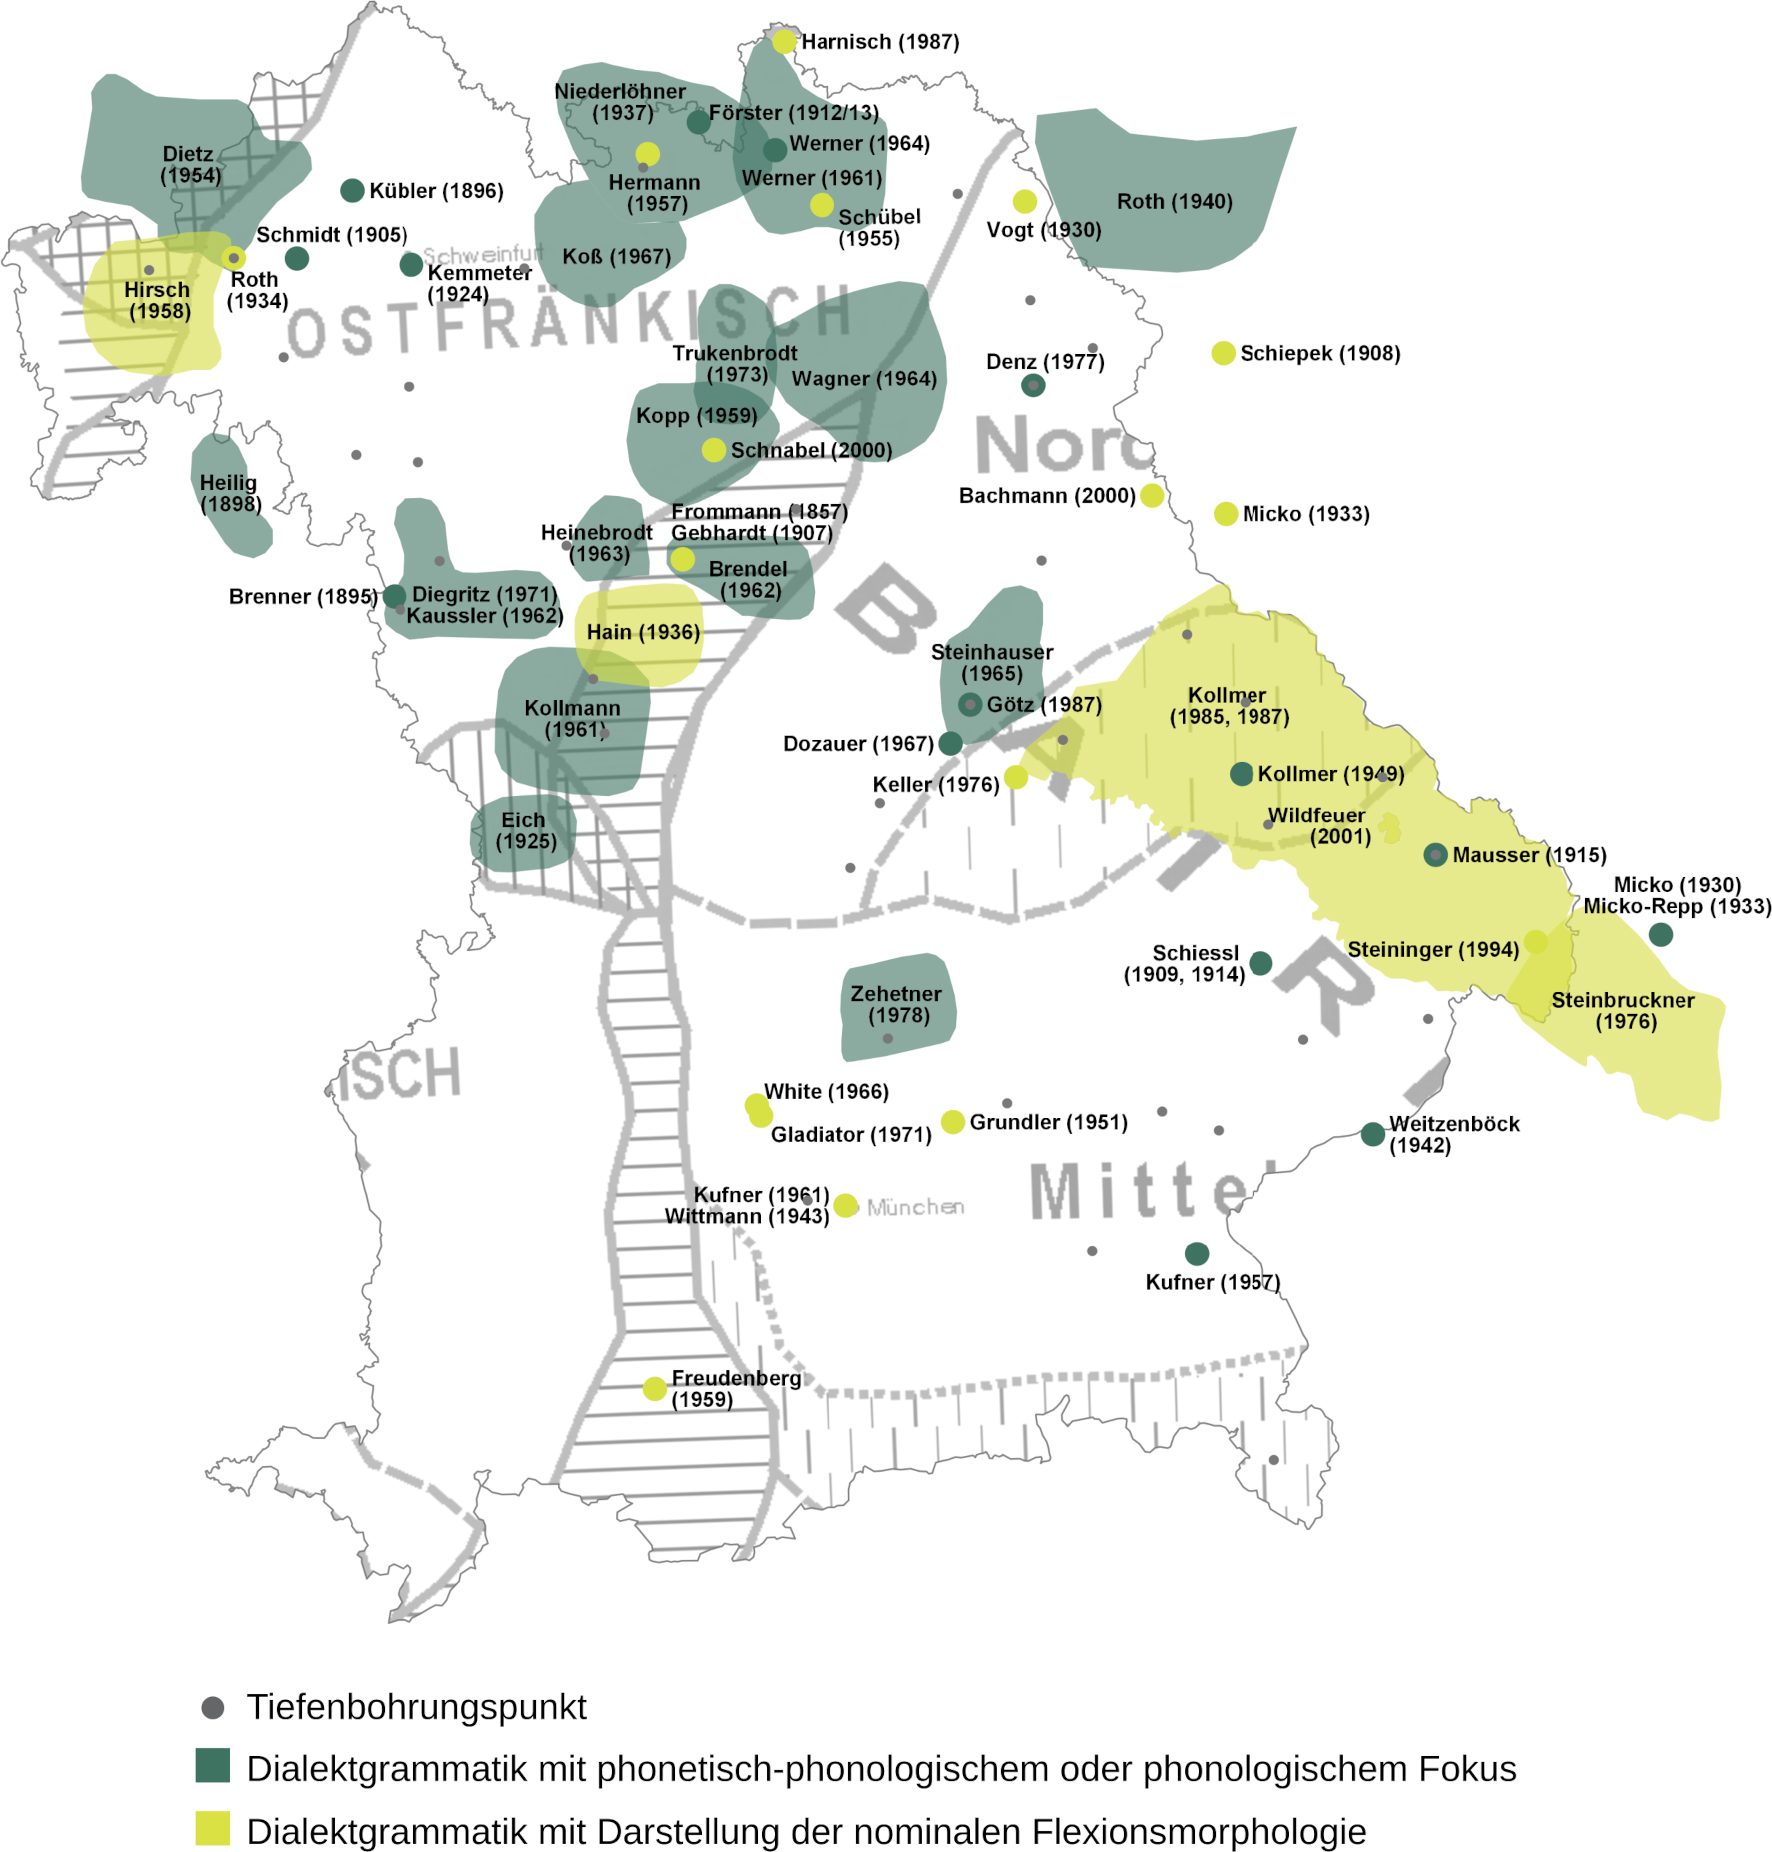
\includegraphics[width=\textwidth]{figures/Karte2.png}
\caption{Dialektgrammatiken zu den oobd. Dialekten Bayerns und \citegen{Wiesinger1983b} Dialekteinteilung}
\label{map:2}
\end{map}

Durch die \textit{Georeferenzierte Online-Bibliographie zur Areallinguistik} (\citealt{SchmidtEtAl2008ff}) ist es möglich, die relevanten dialektologisch-grammatischen Darstellungen im UG zu recherchieren.\footnote{Die \textit{Georeferenzierte Online-Bibliographie zur Areallinguistik} (GOBA) ist Teil des Projekts \textit{regionalsprache.de} und erreichbar über \url{www.regionalsprache.de}. Ich danke zudem den Kolleginnen und Kollegen des Deutschen Sprachatlas in Marburg und des REDE-Projekts für die Möglichkeit und Unterstützung bei der Recherche vor Ort.} Insgesamt wurde eine Auswahl von 65 Ortsmonografien, großräumigeren Landschaftsgrammatiken, Zeitschriftenaufsätzen sowie nicht-publizierten Hochschulschriften und Examensarbeiten ausgewertet (vgl. \mapref{map:2}). Berücksichtigt wurden dabei nicht nur Darstellungen der Flexionsmorphologie, sondern auch Lautlehren, die insbesondere im Oberofr. für ein relativ geschlossenes Gebiet vorhanden sind. Im Kontext einer flexionsmorphologischen Forschungsfrage haben diese zwar meist den Nachteil, dass Basisformen und flektierte Formen nur selten systematisch gegenübergestellt werden, allerdings ist die Darstellung phonologischer Prozesse (in den meisten Fällen ausschließlich oder mit Schwerpunkt im Bereich Vokalismus) mit Blick auf die morphophonologische Perspektive relevant.

\section{Datenaufbereitung und -auswertung}
\label{sec:6.3}
Hauptziel der Analyse ist es, durch den Vergleich von Realisierungsvarianten der Numerus- und Kasusmarkierung in den Ortsdialekten formale Gemeinsamkeiten und Unterschiede sowie -- auf einer übergeordneten Ebene -- Faktoren der Deklinationsklassenzusammensetzung herausarbeiten zu können. Dafür wurden die nicht-typisierten Rohdaten der BSA-Erhebungen als primäre Datenbasis für die 37 Ortspunkte in einer Datenbankanwendung gesammelt, aufbereitet und anschließend hinsichtlich diverser flexivischer und nicht-flexivischer Merkmale analysiert und annotiert (vgl. \sectref{sec:6.3.1}). Zusätzlich wurden im Rahmen der Datenauswertung die Wenker-Materialien und die relevanten Ortsgrammatiken als zusätzliche Evidenz herangezogen.

Die Materialquellen sind sowohl in der Transkription der Dialektbelege als auch in den angewandten Transkriptionsprinzipien ausgesprochen heterogen. Die Transkription der Originalbelege der unterschiedlichen Datenquellen wird sowohl in der Datenbankanwendung als auch in der folgenden Darstellung stets beibehalten und entsprechend interpretiert, um sie in der Analyse aufeinander beziehen zu können.\footnote{Aus Gründen der Lesbarkeit wird bei phonetischen Transkriptionen in der Regel auf die entsprechenden Klammern verzichtet. Mit diesem Ziel erscheinen bei transkribierten Phrasen und Syntagmen auch Leerstellen zwischen den Wortgrenzen.} Trotz einheitlichem Teuthonista-Notationssystem weist auch das BSA-Material von Teilprojekt zu Teilprojekt durchaus gewisse Eigenheiten in der Transkription auf, die ich in der Aufbereitung, insbesondere bei der Annotation der phonologischen und prosodischen Aspekte, zu berücksichtigen hatte (ausführlicher \sectref{sec:6.3.1.2}).

\subsection{Datenbank}
\label{sec:6.3.1}
Für die Dateneingabe und -auswertung wurde eine relationale Datenbank entworfen und mithilfe des Programms \textit{Microsoft Access 2010} aufgebaut. Diese Datenbank steht auf der Website der \textit{Bayerischen Dialektdatenbank} \textit{BayDat} zum Download zur Verfügung (\url{https://baydat.badw.de/materialien/nickel}). Das Format einer relationalen Datenbank wurde zur Datenanalyse und -ausgabe für die Untersuchung gewählt, weil es ein unkompliziertes und flexibles Hinzufügen oder Ändern einzelner Datensätze oder ganzer Annotationskategorien ermöglicht, was bei der Größe des zu untersuchenden Korpus und der Menge der Annotationskategorien von großem Wert und Effizienz war. In der Datenbankanwendung wurden die BSA-Belege aufbereitet und hinsichtlich vorab definierter flexionsmorphologischer, phonetisch-phonologischer, prosodischer, semantischer und außersprachlicher Kriterien analysiert und annotiert (vgl. \sectref{sec:6.3.1.4}). Die Datenauswertung erfolgt in Form von SQL-basierten Abfrageformularen, die das gezielte Sortieren und Durchsuchen der Datensätze zum Beispiel zu einzelnen Flexiven, Pluralmarkierungsverfahren oder einzelnen Konditionierungsfaktoren der Deklinationsklassenzusammensetzung ermöglichen.

\subsubsection{Aufbereitung der BSA-Daten}
\label{sec:6.3.1.1}
Die primäre Datenquelle der Untersuchung, die Rohdaten der Teilprojekte des \textit{Bayerischen Sprachatlas}, sind über die \textit{Bayerische Dialektdatenbank} \textit{BayDat} in einer zentralen Datenbankanwendung digital verfügbar. Zum Zeitpunkt der Datenaufbereitung war die neue und verbesserte Version der \textit{BayDat} noch nicht online; es wurde die nicht mehr aktive Version der Universität Würzburg genutzt.\footnote{Die neue \textit{BayDat}{}-Version ist über die Domain \url{https://baydat.badw.de/} erreichbar. Die nicht mehr aktive Version war über die Adresse \url{http://www.baydat.uni-wuerzburg.de:8080/cocoon/baydat/} verfügbar.} Ausgewertet wurden jene Fragen der Fragebücher der BSA-Teilprojekte, die Flexionsformen des Substantivs oder ganze Nominalphrasen behandeln. Die erhobenen Syntagmen sollten bei der Exploration dazu dienen, verschiedene Flexionsformen zu erheben, die ohne Kontext kaum abzufragen sind (vgl. \citealt[23]{Klepsch2013}). Wurden die Antworten der Gewährspersonen in Form ganzer Syntagmen transkribiert, wurden sie in dieser Form in das eigene Korpus aufgenommen. Mit 8.129 BSA-Datensätzen insgesamt enthält das Korpus Flexionsformen von 271 Lemmata, die entweder in allen der 37 Tiefenbohrungspunkten oder zumindest in einzelnen Teilprojekten abgefragt wurden (vgl. Anhang).

Die Rohdaten liegen in Form von Kodaten der Teuthonista-Transkriptionen der direkten Erhebungen des \textit{Bayerischen Sprachatlas} vor. Für eine elektronische Weiterverarbeitung wurden die handschriftlich transkribierten Belege in den einzelnen BSA-Projekten für jeden einzelnen Erhebungsort in eine \textsc{Ascii}{}-konforme Kodierung umgewandelt (\textit{American Standard Code For Information Interchange}), d.\,h. für die Kodierung der Teuthonista-Transkripte standen nur Zeichen aus dem \textsc{Ascii}{}-Zeichensatz zur Verfügung (näher hierzu \citealt[7--16]{Zimmermann2006}). Infolgedessen setzen sich die Teuthonista-Kodate im Wesentlichen aus Zeichen aus dem lateinischen Alphabet in Kombination mit Ziffern und Sonderzeichen zusammen, die die Diakritika der Teuthonista-Lautschrift abbilden (z.\,B. <a2.> für \teuthoo{a2.}{āͅ}). Als die BSA-Rohdaten in die Online-Plattform \textit{BayDat} eingebunden werden sollten, stellte sich die Schwierigkeit, dass für die Darstellung der Teuthonista-Transkripte in Windows-Systemen die Schriftart \textsc{TeuthoBd} aufgesetzt werden musste, die zwar ebenfalls auf dem \textsc{Ascii}{}-Zeichensatz basiert, aber eine andere Zuordnung der Zeichen verwendet als die Kodierung der Ortsdateien (vgl. \citealt[121]{Zimmermann2006}). Zwar war es möglich, die Kodate der ursprünglichen \textsc{Ascii}{}-Dateien automatisch in Zeichenfolgen für die Schriftart \textsc{TeuthoBd} umzuwandeln und gleichzeitig einige häufig auftretende Kodierfehler automatisch zu korrigieren, aber seltenere Kodierfehler konnten nicht behoben werden, weshalb sich zum Zeitpunkt der Datenaufbereitung dieser Untersuchung noch immer fehlerhafte Kodate in den \textit{BayDat}{}-Rohdaten finden ließen. 

Neben den potenziellen Kodierfehlern bestand zum Zeitpunkt der Datenaufbereitung eine weitere Schwierigkeit darin, dass die Ausgabe der Belege in \textit{BayDat} teilweise fehlerhaft ist.\footnote{Obwohl die Frage im entsprechenden Teilprojekt abgefragt wurde, erscheint die Meldung „Frage in diesem Projekt/Ort nicht erhoben“ oder es wird -- bei falscher Zuordnung von Fragenummer und Antwortbeleg -- ein anderer, nicht der Frage zugehöriger Beleg angezeigt. Die genannten Nachteile der alten \textit{BayDat}{}-Version werden im Zuge der Neu-Aufsetzung der \textit{BayDat} sukzessive behoben, was zukünftige Datenaufbereitungen erheblich erleichtern dürfte.} In beiden Fällen wurde das Vorhandensein der Belege in den Original-Fragebüchern der jeweiligen Untersuchungsorte überprüft und ggf. händisch kodiert. Auch nach manueller Überprüfung und Korrektur der Kodate ist mit einer gewissen Fehlerquote zu rechnen; diese Kodierfehler betreffen in erster Linie die Diakritika in der Teuthonista-Notation und damit phonetische Feinheiten, z.\,B. wie geschlossen ein /e/ realisiert wurde. Dies ist im Kontext einer morphologischen Untersuchung weniger schwerwiegend als in einer phonologischen, da hier v.\,a. relevant ist, dass dieses \textit{e} die Numerusinformation in Form eines Umlauts markiert. Sind Diakritika (z.\,B. bei der Notation von Vokalquantitäten) für das Pluralmarkierungsverfahren entscheidend, wurden im Zweifelsfall die Originaltranskripte zum Vergleich herangezogen.

\subsubsection{Typisierung der Teuthonista-Transkripte}
\label{sec:6.3.1.2}
Trotz des einheitlichen Teuthonista-Notationssystems gibt es in den einzelnen Teilprojekten des BSA Abweichungen im Transkriptionsverfahren und Spezifika einzelner Exploratoren (vgl. \citealt[22]{SNiB1}). Die große Stärke der Teuthonista-Notation, sämtliche phonetische Feinheiten abbilden zu können, wirft im Rahmen einer flexionsmorphologischen Untersuchung methodische und sprach\-sys\-tematische Fragen auf: Wann repräsentiert eine phonetisch differente Form zwischen Singular- und Pluralbeleg auch einen phonemischen Unterschied, der eine morphologische Unterscheidung kodiert? Wann handelt es sich um rein phonetische Variation ohne Funktionalität? Die Feinheit des Notationssystems mit beispielsweise vier Abstufungen der Vokalquantität und fünf Differenzierungen von Lenis- bzw. Fortisobstruenten stellt in der Praxis der Annotation von Pluralmarkierungsverfahren damit eine nicht geringe methodische Schwierigkeit dar, wie die Beispiele \REF{ex:6:1} und \REF{ex:6:2} illustrieren:

\ea\label{ex:6:1} \teuthoo{dA}{dα} \teuthoo{hu.2nd}{hūͅnd} – \teuthoo{dhu.nt5}{dhuͅnt̩} (‚Hund‘, Bernhardswald)
\ex\label{ex:6:2} \teuthoo{ha.2d}{hāͅd} – \teuthoo{he:<8d5}{hê{\doubleogonek}\klammerobenpost{}d̩} (‚Haut‘, Grafenkirchen)
\z

Es finden sich jeweils Kontraste in der Stammvokalquantität sowie Lenis"=Fortis"=Kontraste im Stammauslaut. Während die Kontraste in \REF{ex:6:1} zwischen Lang- und Kurzvokal respektive zwischen Lenis und leicht lenisierter Fortis bestehen, ergibt sich der Kontrast in \REF{ex:6:2} in der Notation eines Langvokals im Singular vs. einer eingeklammerten Halblänge im Plural, im Konsonantismus besteht der Kontrast zwischen Lenisplosiv vs. leicht fortisiertem Lenisplosiv. In der Annotation muss nun gewichtet werden, ob die z.\,T. minimale Variation, die transkribiert wurde, gleichermaßen als Beleg der Pluralmarkierungsverfahren Vokalquantitätskontrast und Lenis-Fortis-Kontrast klassifiziert werden kann oder ob es sich um eine rein phonetische Variation handelt, die aus Perspektive der Flexionsmorphologie vernachlässigt werden kann. Während der Bearbeitung der BSA-Bände bestanden ähnliche methodische Fragen, da die Transkripte auch für die Kartierung der Varianten typisiert werden mussten. Die folgenden Prinzipien der eigenen Typisierungs- und Klassifizierungspraxis orientieren sich daher an den Prinzipien des BSA (vgl. \citealt[6]{SMF2.1}, \citealt[18]{SUF1}):\largerpage

\begin{itemize}
\item Geklammerte Diakritika, z.\,B zur Markierung des Öffnungsgrades von Vokalen, werden wie ungeklammerte Diakritika behandelt, d.\,h. die Transkription \teuthoo{a)4}{a\klammeruntenpost{}̣} wird wie die Transkription \teuthoo{a4}{ạ} gewertet.\footnote{Reduzierungen von Grundzeichen und Diakritika in Form von Hochstellung des entsprechenden Zeichens (z.\,B. o\textsuperscript{α}) können (mit Ausnahme von <ʰ>) in der Schriftart \textsc{TeuthoBD} nicht dargestellt werden und konnten -- anders als in den BSA-Publikationen -- bei der Datenanalyse daher nicht berücksichtigt werden. Doppelt reduzierte Grundzeichen und Diakritika (z.B. \teuthoo{o}{o}\textsuperscript{(\teuthoo{a}{a})} wurden etwa im SMF als nicht vorhanden gewertet, diese Form der Notation kann in den \textsc{TeuthoBD}{}-Kodaten jedoch nicht mehr nachvollzogen werden.}
\item Halblängen (â) werden wie ganze Längen (ā) behandelt, d.\,h. im Beispielbeleg \REF{ex:6:2} würde kein Quantitätskontrast annotiert werden.
\item Vokalkürze wurde i.\,d.\,R. nicht gesondert notiert (Notation \teuthoo{a}{a}), in „besonderen (unerwarteten) Fällen“ (\citealt[163]{SBS1}) wurde Vokalkürze notiert (Diakritikum \teuthoo{a3}{ă}). Beide Notationen werden gleichermaßen als Kurzvokale behandelt.
\item Zwischenwertnotationen („Burger“) werden dem unteren Bestandteil zugeordnet, d.\,h. das Suffix \teuthoo{Å}{{\burgershwaalpha}} in der Pluralform \teuthoo{he94mÅd5\_Å}{he\klammeruntenpost{}̣m{\burgershwaalpha}d̩ʰ{\burgershwaalpha}} (‚Hemden‘, Mitteleschenbach) wird als α gewertet.
\item Abstufungen bei Lenes und Fortes werden als zweigliedriges Oppositionssystem behandelt: Lenes= \teuthoo{d;}{d͓͓} – \teuthoo{d,}{d͓} – \teuthoo{d}{d} – \teuthoo{d5}{d̩} – \teuthoo{d\%}{d͈}, Fortes= \teuthoo{t;}{t͓͓} – \teuthoo{t,}{t͓} – \teuthoo{t}{t} – \teuthoo{t5}{t̩} – \teuthoo{t\%}{t͈}. Die transkribierte Differenz in \REF{ex:6:2} würde damit nicht als Fortisierung annotiert, beide Plosive im Auslaut als Lenes behandelt werden (siehe hierzu auch \sectref{sec:7.1.2.3.1}).
\item Die Notationen \teuthoo{B}{{\btilde}} und \teuthoo{æ}{{\burgerbw}} werden (neben den Frikativen \teuthoo{w}{w}, \teuthoo{v}{v}) als Spirantisierungen von \teuthoo{b}{b} annotiert, z.\,B. \teuthoo{go<we}{ɡôwe} -- \teuthoo{gðo9.æe4n}{ɡ̩o\klammeruntenpost{}ͅ{\burgerbw}ẹn} (‚Gabel‘, Neukirchen am Inn)
\end{itemize}

\subsubsection{Mehrfachbelege und Variation im Datenmaterial}
\label{sec:6.3.1.3}
Im Normalfall wurde für jede Frage nur ein Antwortbeleg transkribiert. Wurden im Fragebuch mehrere Varianten transkribiert, so wurden diese entweder als eigene Datensätze in die Datenbank aufgenommen oder (v.\,a., wenn es sich um Aussprachevarianten handelte, die keine differente Form der Pluralmarkierung aufweisen) im Feld „Bemerkung“ des Formulars \textit{BSA-Belege} dokumentiert. Wenn für einen Untersuchungsort verschiedene Flexionsformen belegt waren, so erschien es von Anfang an sinnvoll, diese als eigene Datensätze in das Korpus aufzunehmen, da es sich um Belege intra-individueller oder (wenn mehrere Gewährspersonen beteiligt waren) inter-individueller Variation im Ortsdialekt handelte (siehe \citealt{Nickel2021}). Waren solche Varianten im Rohmaterial belegt, wurde stets im Originalfragebuch nachgeschlagen, ob es Exploratorenkommentare zu den varianten Formen gab, z.\,B. „spontan“, „Erinnerungsform“, „hochdeutsch“ o.\,ä. (vgl. \citealt[165f.]{SBS1}) Die Exploratorinnen und Exploratoren waren angehalten, insbesondere bei „lichtscheuen“ (Zitat aus den \textit{Grundsätzen für Sprachatlasaufnahmen} von Robert Hinderling, zitiert nach \citealt[48]{Schmuck2014}), d.\,h. schwer zu elizitierenden Lauten und Formen auf Selbstkorrekturen der Gewährspersonen zu achten und diese als solche kenntlich zu machen. Hat sich die Gewährsperson korrigiert, so wurde der korrigierte Beleg als Datensatz aufgenommen, der (Spontan-)Beleg wurde in das Feld „Bemerkungen“ aufgenommen und als solcher gekennzeichnet. Außerdem wurden die Kommentare der Exploratoren in das Feld „Bemerkungen“ aufgenommen, da sie Hinweise für eine Verortung der varianten Formen in der horizontalen oder vertikalen Dimension sind.

\subsubsection{Datenannotation und -auswertung}
\label{sec:6.3.1.4}
Den Untersuchungsgegenstand stellen das Substantiv und die syntaktische Einheit Nomi\-nal\-phrase bestehend aus Definitartikel und Substantiv dar. In die Datenbankanwendung wurden die BSA-Transkripte (Nom.Sg. und Nom.Pl. des Substantivs, ggf. Formen der obliquen Kasus und Diminutivformen) als isolierte Belege oder ganze Nominalphrasen eingepflegt, lemmatisiert und mit der Information zum Erhebungsort verknüpft. Die Analyse der Daten erfolgte durch die Annotation verschiedener flexionsmorphologischer und nicht-flexivischer Merkmale. Zur Analyse der Flexion gehören die konkreten Pluralmarker, aufgeschlüsselt nach möglichen Kontrasten im Vokalismus (Qualität und Quantität), im Konsonantismus sowie möglichen Suffixen, dem abstrahierten Typ des Pluralkodierungsverfahren (Null, additiv, modulativ oder die diversen kombinierten Verfahren) sowie der dialektalen Deklinationsklasse. Neben der Analyse der Pluralallomorphie besteht das zweite Untersuchungsziel darin, die Konditionierungsfaktoren der Deklinationsklassenzusammensetzung im Flexionssystem der Tiefenbohrungspunkte herauszuarbeiten. Der Analyseaspekt knüpft an die Forschung zur Konditionierung von Deklinationsklassen und Deklinationsklassenwandel im Schriftdeutschen und in den Dialekten an. Die Kategorien der Datenannotation bilden die Ergebnisse des aktuellen Forschungsstandes ab, indem folgende mögliche Konditionierungsfaktoren ausgewertet werden: Genus,\footnote{Liegt der Dialektbeleg in Form einer Nominalphrase mit Artikel vor, wurde die Form des Artikels hinzugezogen, um die Genuszugehörigkeit des Lexems im Ortsdialekt analysieren zu können. Wurde das Genus des Lexems durch einen metasprachlichen Kommentar angegeben, ist dies ebenfalls berücksichtigt. Stehen weder morphosyntaktischer Kontext noch metasprachliche Angaben zur Verfügung, musste das Genus ausgehend vom Standard oder unter Berücksichtigung von Dialektgrammatiken oder vorhandenen Sprachatlanten annotiert werden. Die dialektale Genuszugehörigkeit gilt dann nicht als gesichert und wird durch Einklammerung der Genuszuweisung („(fem.)“, „(mask.)“, „(neutr.)“) markiert.} prosodisch"=phonologische Aspekte (u.\,a. Silbenanzahl und -auslaut), morphologische Aspekte (Wortbildung, Singularstammform) sowie semantische Merkmale. Durch den Aufbau der Datenbank und die differenzierte Form der Annotation  ist es möglich, die Dialektbelege nach einzelnen Merkmalen (z.\,B. Pluralmarkierung bei Kontraktion des Singularstammes) oder einer Kombination von Merkmalen (z.\,B. Pluralmarkierung von \textit{n}{}-erweiterten Substantiven mit kontrahiertem Singularstamm) in den Auswertungsformularen zu sortieren und anzuzeigen. Die Abfrageformulare ermöglichen es, -- je nach Einstellung des Filters -- die absolute Anzahl der relevanten Belege abzulesen. Weitere statistische Auswertungen erfolgten dann außerhalb der Datenbankanwendung.

\subsection{Kartierung}
\label{sec:6.3.2}
Die Auswertungen werden durch Sprachkarten ergänzt, um die areale Dimension der Variation, und möglicherweise die Dialektspezifik einzelner Phänomene zu visualisieren. Diese Sprachkarten sind ein Instrument der Datenauswertung, sie sind daher weniger Untersuchungsziel an sich als ein Zwischenergebnis. Zur Kartierung wurden Beleglisten aus der \textit{Access}-Datenbankanwendung in das Tabellenkalkulationsprogramm \textit{Excel} exportiert und für die Kartierung aufbereitet. Die Erstellung der Karten erfolgte mit dem \textit{REDE SprachGIS} (\citealt{SchmidtEtAl2008ff}), das den Import von Datensätzen im CSV-Format und damit auch das automatische Kartieren der eigenen Beleglisten ermöglicht.\footnote{Die Farbgebung der Karten basiert stets auf den durch die Anwendung \textit{iWantHue: Colors for data scientists} (\url{https://medialab.github.io/iwanthue/}) empfohlenen Farbspektren für distinkte Farben.}

\part{Dialektgeografischer Teil}
\label{part:II}
\noindent Die folgende Darstellung der nominalen Flexionsmorphologie in den oobd. Dialekten Bayerns knüpft an die in Teil~\ref{part:I} aufgezeigten Forschungsbefunde und "=fra\-gen zu dialektalen Deklinationsklassensystemen und zur Numerus- und Kasusmarkierung an. Ziel ist es, das Deklinationsklassensystem dieser Dialekte kontrastiv darzustellen (und zwar im interdialektalen Vergleich und in der diachronen Entwicklung) und gleichzeitig auf der Formenebene dialektale und eventuell dialektraumspezifische Kodierungsverfahren zu beschreiben. Teil~\ref{part:II} ist dabei spiegelverkehrt zu Teil~\ref{part:I} aufgebaut: Ausgehend von Markierungsstrategien und konkreten Markern wird das Deklinationsklassensystem der oobd. Dialekte analysiert. Grundlegend ist hierbei das Verständnis von Flexion als grammatischem Schnittstellenphänomen. Das Leitthema der folgenden Kapitel lautet daher -- in Anlehnung an \citet[13]{Harnisch1987} -- \textit{Where’s} \textit{morphology?}


Ziel ist es, die Flexion innerhalb des Sprachsystems der jeweiligen Ortsdialekte darzustellen und aufzuzeigen, wo Morphologie mit anderen Systemebenen interagiert (und zwar mit Blick auf Synchronie und Diachronie) und wo Morphologie unabhängig stattfindet. Im Einzelnen ist die Untersuchung dabei durch folgende Forschungsfragen motiviert:

\begin{itemize}
\item Flexion zwischen \textit{Phonologie} \textit{und} \textit{Morphologie}: Inwiefern sind die Markierungsverfahren und einzelnen Marker in den rezenten oobd. Dialekten das Ergebnis dialektspezifischer phonologischer Prozesse (etwa von Apokope oder Vokaldehnung)? Inwiefern bedingen sich hier phonologischer und morphologischer Wandel? Und in welchem Maße werden phonologische Alternationen morphologisiert und produktiv?
\item Wo löst \textit{morphologischer} \textit{Wandel} (z.\,B. in Form von innerparadigmatischen Ausgleichsprozessen) weiteren morphologischen Wandel aus, wie es beispielsweise im Bair. mit den „potenzierten“ Pluralen und im Niederdeutschen mit dem \textit{s}{}-Plural bei Nasalsuffix im Nom.Sg. geschehen ist (siehe \sectref{sec:4.2.1})?
\item Flexion zwischen \textit{Morphologie} \textit{und} \textit{Syntax}: Wo und in welchem Umfang wird die Numerus- und die Kasusinformation in der Nominalphrase markiert, wenn sie am Substantiv abgebaut ist? Inwiefern werden Synkretismen bei Artikelformen durch formale Kodierung am Substantiv kompensiert?
\item Flexion zwischen \textit{Morphologie} \textit{und} \textit{semantisch-pragmatischem} \textit{Kontext}: In welchem Maß ist die formale Kodierung flexivischer Information von der Eindeutigkeit des Kontexts abhängig? Wird die Numerus- oder Kasusinformation disambiguiert, wenn der Kontext ambig ist? Wie „statisch“ oder variabel ist also Flexion im Äußerungskontext?
\end{itemize}

Die Darstellung der Formenbildung ist zunächst -- so weit wie möglich -- theorieneutral, eine Diskussion der dialektalen Flexionsmorphologie vor dem Hintergrund verschiedener morphologischer Theoriebildungen erfolgt erst in \chapref{chap:10}. Allerdings liegen der deskriptiven Analyse die theoretischen Vorannahmen einer prozessorientierten Morphologie zugrunde, die etwa bei Nullpluralen von einem morphologischen Verfahren ausgeht (vgl. \chapref{chap:4}).


Das Ziel besteht also nicht darin, dialektale Flexionsmorphologie vor dem Hintergrund eines regelbasierten Ansatzes zu modellieren, wie etwa \citet{Harnisch1987} im Rahmen der Natürlichen generativen Morphologie. Stattdessen werden die synchronen morphologischen Strukturen, die in den Dialektdaten zu finden sind, erfasst und diachron eingeordnet. Hierin folgt die Untersuchung der Pionierarbeit von \citet{Rowley1997}, der die nominale Flexion der ofr. und nordbair. Dialekte Nordostbayerns synchron-deskriptiv darstellt und gleichzeitig „diachron erklärend sein will“ \citep[2]{Rowley1997}. Methodisch knüpft die vorliegende Untersuchung dabei an \citegen{Rowley1997} Arbeit an und weitet die Analyse zur flexionsmorphologischen Sprachgeografie auf weitere Dialekträume, Analyseaspekte und Datenmaterial aus.
 % Teil II
\chapter{Formenbildung des Substantivs in den ostoberdeutschen Dialekten Bayerns}\label{chap:7}
\addtocontents{toc}{\protect\enlargethispage{1\baselineskip}}

\begin{quote}
Eine vollständige Darstellung sollte nicht nur zeigen, was es alles gibt, sondern auch klar machen, welche Erscheinungen es trotz guter Voraussetzungen nicht gibt.\hbox{}\hfill\hbox{\citep[348]{Rowley2004}}
\end{quote}

Im ersten Teil der Datenauswertung steht die Formenbildung des Substantivs im Zentrum, im zweiten Teil werden das dialektale De\-kli\-na\-tions\-klas\-sen\-sys\-tem und Faktoren der Deklinationsklassenzusammensetzung in den untersuchten Dialekten fokussiert (\chapref{chap:8}).

Die synchrone Analyse der Formenbildung der Flexionskategorien Numerus (\sectref{sec:7.1}) und Kasus (\sectref{sec:7.2}) bezieht sich auf das Wort im Paradigma und steht damit in der Tradition der Word-and-paradigm-Morphologie im Sinne \citegen{Hockett1954}. Morphologische Kodierung von Merkmalen einer Flexionskategorie wird damit immer relational verstanden, die Analyse erfolgt durch den Vergleich der Grundform und der im Paradigma vorkommenden flektierten Formen (vgl. \citealt[26--29]{Harnisch1987}, \citealt[23--25]{Rowley1997}). \citet[28]{Harnisch1987} verknüpft Word-and-paradigm-Morphologie und Sprachverwendung, indem er annimmt, „daß sowohl das Kodieren durch den Sprecher wie das Dekodieren durch den Hörer auf einem solchen Nebeneinanderhalten von Basis und Flexionsform aufbaut“ -- ein Gedanke, der sich konzeptuell in den Schemata zweiter Ordnung wiederfindet (\sectref{sec:5.3.3}). Jeder formale Unterschied im synchronen Paradigma, der sich durch den Vergleich von Basis- und flektierter Form im Paradigma ergibt, symbolisiert die Kodierung flexivischer Information und kann unterschiedlichen morphologischen Kodierungsverfahren zugeordnet werden: segmentierbare, additive Markierung (\teuthoo{le2b}{lēb} -- \teuthoo{le2br}{lēbr} ‚Laib‘ in \tabref{tab:15}), stammaffizierende Verfahren in Form lautlicher Kontraste des Vokalismus oder Konsonantismus am Stamm selbst (und zwar in verschiedenen Ausprägungen in den untersuchten Dialekten) oder Nullmarkierung (vgl. (1) und (2) in \tabref{tab:15}).


\begin{table}
\begin{tabularx}{\textwidth}{l@{~~}>{\raggedright\arraybackslash}p{.28\textwidth}llQ}
\lsptoprule
& Ortsdialekt & Nom.Sg. & Nom.Pl. & in\-ner\-pa\-ra\-dig\-ma\-ti\-sche

Alternationen --

Ko\-die\-rungs\-ver\-fah\-ren \\
\midrule
(1) & ofr. Erlabrunn & \teuthoo{le.2b}{lēͅb} & \teuthoo{le.2br}{lēͅbr} & additiv\\
\tablevspace
& nordbair.

Win\-disch\-eschen\-bach & \teuthoo{lo<Ab}{lôαb} & \teuthoo{lo2i}{lōi} & stammaffizierend

(Vokalqualität,

Kon\-so\-nan\-tis\-mus\-kon\-trast)\\
\tablevspace
& mittelbair. Wald\-hof & \teuthoo{lo<4Ab}{lộαb} & \teuthoo{lo<4Ab}{lộαb} & Null\\
\midrule
(2) & ofr. Erlabrunn & \teuthoo{hu2nd}{hūnd} & \teuthoo{hu?.nd5\_}{hüͅnd̩ʰ} & stammaffizierend

(Vokalquantität, {}-qualität)\\
\tablevspace
& nordbair.

Win\-disch\-eschen\-bach & \teuthoo{A}{α} \teuthoo{hu>(+nd5\_}{hû̃\klammerobenpost{}nd̩ʰ} & \teuthoo{hu3nt\_}{hŭntʰ} & stammaffizierend

(Vokalquantität,

Kon\-so\-nan\-tis\-mus\-kon\-trast)\\
\tablevspace
& mittelbair. Wald\-hof & \teuthoo{a4}{ạ} \teuthoo{hund5\_}{hund̩ʰ} & \teuthoo{hu94nt\_}{hu\klammeruntenpost{}̣ntʰ} & stammaffizierend

(Kon\-so\-nan\-tis\-mus\-kon\-trast)\\
\lspbottomrule
\end{tabularx}
\caption{Morphologische Kodierungsverfahren an den Beispielen \textit{Laib} und \textit{Hund} im UG\label{tab:15}}
\end{table}

Auch der Ausgangspunkt der diachronen Perspektive ist das Paradigma, da synchrone Formen und Paradigmenkonstellationen nur so erklärt werden können. So sind synkretische Pluralformen wie \teuthoo{e.2mA94sn@}{ēͅmα\klammeruntenpost{}̣sn̥} -- \teuthoo{e.2mA94sn@}{ēͅmα\klammeruntenpost{}̣sn̥} ‚Ameise‘ (ofr. Burgbernheim) oder \teuthoo{dA}{dα} \teuthoo{e?9.b5v5l.}{ë\klammeruntenpost{}ͅb̩v̩lͅ} -- \teuthoo{e?(9.b5v5l@}{ë\klammerobenpost{}\klammeruntenpost{}ͅb̩v̩l̥} ‚Apfel‘ (ofr. Hallerstein) in den rezenten Dialekten historisch durch das Eindringen eines Flexivs in die Grundform des Nom.Sg. entstanden. Nur durch den Einbezug des Paradigmas können die rezenten Nullplurale als Ergebnis von morphologischem Ausgleich erklärt werden. Das Paradigma erweist sich hier „als bedingender Faktor beim Sprachwandel“ \citep[25]{Rowley1997}.

Aus der rein synchronen Analyse und mit Blick auf die Leitfrage „Where’s morphology?“ stellt sich für die verschiedenen stammaffizierenden Verfahren in 	\tabref{tab:15} die Frage: Was ist hier eine rein phonologisch bedingte Alternation, und wo ist die Alternation genuin morphologisch, d.\,h. funktionalisiert und evtl. sogar produktiv? Dass die Lösung dieses Problems nicht trivial ist, zeigen sowohl regelbasierte Ansätze (etwa \citealt{Seiler2008} oder \citealt{Harnisch2016}) als auch deskriptive Analysen (z.\,B. \citealt{Birkenes2014}).

Bei der Verortung morphophonologischer Alternationen an der Schnittstelle von Phonologie und Morphologie (und zur Formulierung von Regularitäten) braucht es -- in Anlehnung an \citet[97--98]{Harnisch2016} -- für eine rein synchrone Lösung die Berücksichtigung (1) des phonologischen Systems des Dialekts, (2) der „spezifischen Paradigmenstrukturbedingungen“ und (3) funktionelle Faktoren (in diesem Fall die Kodierung flexivischer Information). Diese drei Analyseebenen gelten auch für eine rein deskriptive Lösung, doch liegt in meinen Augen der entscheidende Punkt in der mentalen Repräsentation, d.\,h. in der kognitiven Verankerung dieser morphophonologischen Alternationen. In welchem Maße symbolisieren innerparadigmatische Alternationen die flexivische Information? Gibt es überhaupt Alternationen, die rein phonologisch bedingt sind und die keinerlei morphologische Information symbolisieren? Im Falle des Umlauts wurden in der Forschung zwei Prozesse diskutiert, die den Übergang von einer phonologischen Alternation zu einer morphologischen Symbolisierung markieren: die Vokalreduktion in den Endsilben und innerparadigmatischer Ausgleich, d.\,h. die Tilgung phonologisch bedingter Umlaute im Singularparadigma (siehe \sectref{sec:3.1.1}). Offen bleibt dabei, in welchem Maße der Umlaut bereits vor der Funktionalisierung als produktiver Pluralmarker die flexivische Information mitangezeigt hat. \citet[196]{Seiler2008} formuliert diesen Aspekt so, dass sich „das Sprecherhirn verhältnismäßig gut Kookkurrenzen, aber verhältnismäßig schlecht Kausalitäten merken kann.“ Das heißt, das ahd. Sprecherhirn erfasst die Kookkurrenz von Umlautalternanz und Pluralsuffix -\textit{ir} oder -\textit{i} (und damit die morphologische Pluralinformation), nicht aber, dass die Alternanz durch das \textit{i}{}-haltige Suffix verursacht wurde. Solange ungeklärt ist, wie stark Phonologie und Morphologie in der mentalen Repräsentation tatsächlich modularisierte Systeme darstellen (oder eben nicht), spricht m.\,E. nichts dagegen, innerparadigmatische Alternationen wie \teuthoo{hu2nd}{hūnd} -- \teuthoo{hunt}{hunt} oder \teuthoo{loAb}{loαb} -- \teuthoo{loi}{loi} im Phänomenbereich der Morphologie zu verorten und sie aus der Perspektive morphologischer Kodierung zu beschreiben (vgl. \citealt[35]{Rowley1997}).

Die folgenden Kapitel zur Formenbildung (insbesondere \sectref{sec:7.1.2} zur stammaffizierenden Markierung) werden zeigen, dass es sinnvoll und praktikabel ist, eine Skala für diese Alternationen anzunehmen. Ein Pol entspricht lexikalisierten morphophonologischen Alternationen, wie sie etwa \citet{Birkenes2014} für subtraktive Pluralformen beschreibt. Diese Formen sind nicht mehr aus synchronen phonologischen Regeln abzuleiten, sondern konservieren historische phonologische Prozesse. Damit symbolisieren Formen wie \teuthoo{loAb}{loαb} -- \teuthoo{loi}{loi} synchron die flexivische Information und ermöglichen -- bei höherem Speicheraufwand -- einen direkten Zugriff auf die lexikalisierten Flexionsformen \citep[59]{Harnisch1990}. Den anderen Pol bilden produktive morphophonologische Alternationen, die unabhängig von phonologischen Kontextbedingungen funktionalisiert sind: als prominentestes und produktivstes Verfahren der Umlaut (\teuthoo{hund}{hund} -- \teuthoo{hu?nd}{hünd}) und -- zumindest teilweise im Bair. -- Pluralformen des Typs \teuthoo{hu2nd}{hūnd} -- \teuthoo{hunt}{hunt}.

Diese grundsätzlichen Überlegungen fokussieren stärker die funktionale Seite morphophonologischer Alternationen im Flexionsparadigma der rezenten Dialekte. Im Zentrum der folgenden Kapitel steht zunächst primär die Formenseite: Welche formalen Marker werden genutzt, um flexivische Informationen zu kodieren? Gibt es areale Unterschiede in den Markierungsstrategien, gibt es dialektspezifische Marker? Das phonologische System eines (Orts-)Dialekts steuert das zur Verfügung stehende Markerinventar, das Vorhandensein und die konkrete Realisierung von einzelnen Kodierungsverfahren sind in hohem Maße vom Eintreten phonologischer Prozesse abhängig. Die folgende Darstellung der einzelnen Verfahren geht daher von den spezifischen phonologischen Voraussetzungen aus, um Gemeinsamkeiten und Unterschiede der Numerus- und Kasusmarkierung im oobd. Dialektraum zu kontrastieren und um das Nebeneinander synchroner Formen wie \teuthoo{loAb}{loαb} -- \teuthoo{loAb}{loαb} und \teuthoo{loAb}{loαb} -- \teuthoo{loi}{loi} zu erklären. Dabei gehen die Darstellungen da in die Tiefe und ins Detail, wo es darum geht, die komplexe Interaktion von Phonologie und Morphologie herauszuarbeiten und aufzuzeigen, wie diese diachron zur Herausbildung von dialekt(raum)spezifischen Flexionsmustern und Markierungsverfahren geführt hat. Da die einzelnen phonologischen Prozesse die Dialekte unterschiedlich affizieren, sind zum Teil ortsdialektspezifische Darstellungen nötig, die mit Blick auf die Deklinationsklassen in \chapref{chap:8} gebündelt und in \chapref{chap:10} interpretiert werden.

\section{Pluralmarkerinventar und phonologische Voraussetzungen}
\label{sec:7.1}
Die Zusammenschau der Kodierungsstrategien in den untersuchten Dialekten geht von den Kodierungstypen aus: additive und stammaffizierende Verfahren, Nullmarkierung sowie suppletive Verfahren. Zudem treten im Untersuchungsgebiet verschiedene Markierungsverfahren kombiniert auf. Die konkrete formale Realisierung der Pluralmarkierungstypen (d.\,h. die Pluralmarker) variiert hingegen in den untersuchten Dialekten und ist z.\,T. areal\-bildend, es handelt sich also um Heteromorphie.

\subsection{Additive Pluralmarkierung}\label{sec:7.1.1}
\begin{sloppypar}
Additive Pluralmarkierung besteht in der Verkettung (Konkatenation) von Stamm und Suffixen, die die flexivische Information tragen. Anders als bei stammaffizierenden (d.\,h. nicht-konkatenativen) Verfahren ist der Träger der grammatischen Information vom Träger der lexikalischen Information segmentierbar, die „Integrität des Stammes“ \citep[182]{Seiler2008} bleibt gewahrt.
\end{sloppypar}

\begin{map}
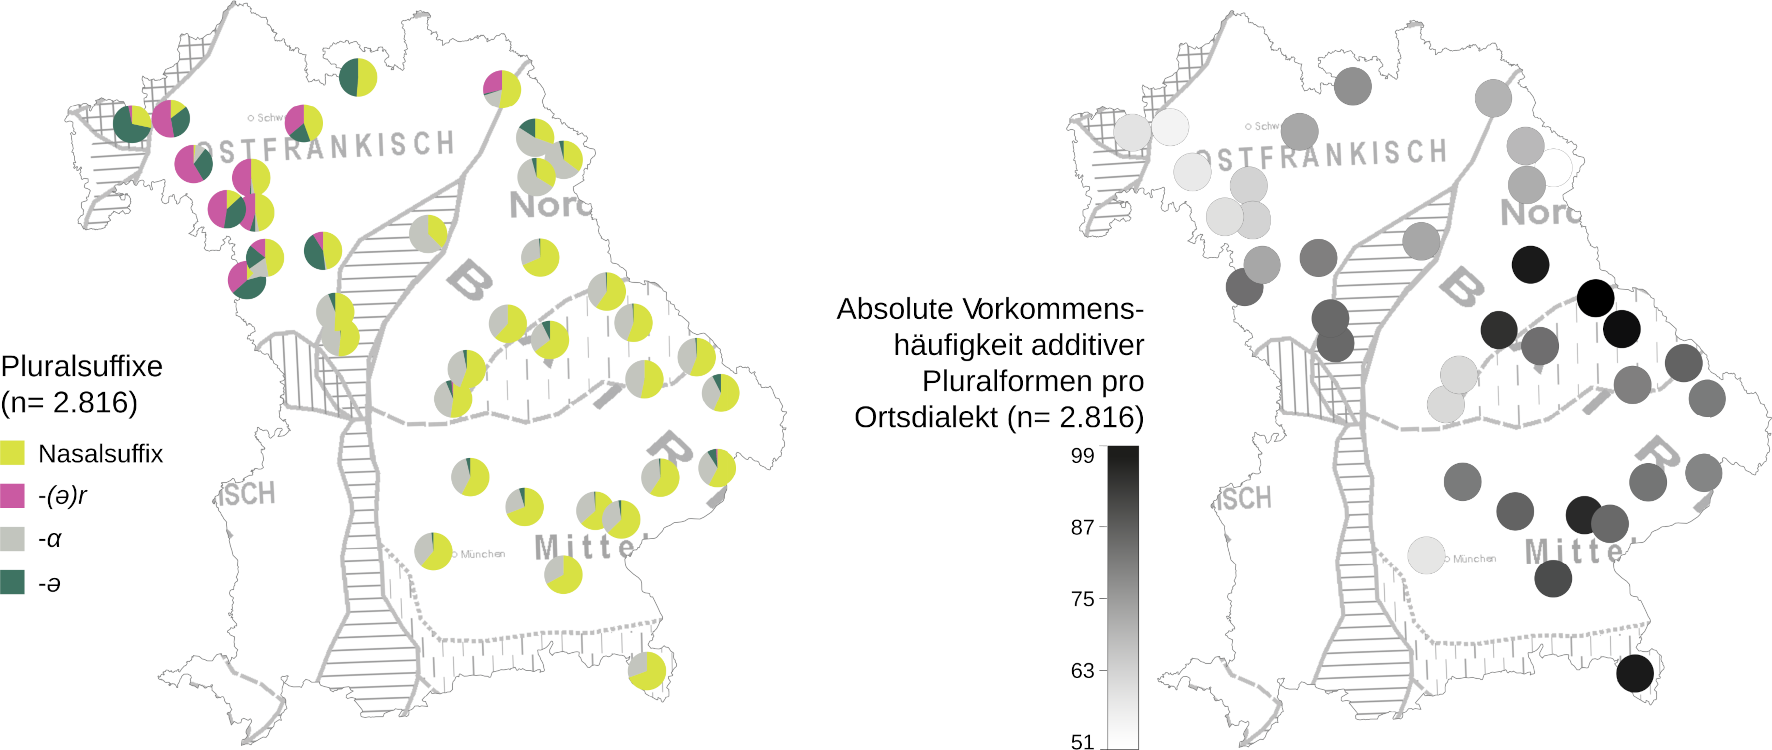
\includegraphics[width=\textwidth]{figures/Karte3.png}
\caption{Häufigkeitsverteilung der Pluralsuffixe und Chloroplethkarte der absoluten Vorkommenshäufigkeit additiver Pluralmarkierung}
\label{map:3}
\end{map}

\mapref{map:3} illustriert, dass additive Pluralmarkierung hinsichtlich der Distribution der einzelnen Pluralsuffixe dialektspezifisch ist (vgl. \sectref{sec:7.1.1.1}). Daneben bestehen areale Unterschiede in der absoluten Vorkommenshäufigkeit additiver Pluralformen, wie die Chloroplethkarte zeigt.

An dieser Stelle ist es sinnvoll, auf Genus als Konditionierungsfaktor von Deklinationsklassen vorzugreifen, da das Raumbild durch den relativen Anteil additiver Pluralmarkierung bei Feminina zu erklären ist (vgl. \sectref{sec:8.3.1.3}). Die Mosaik-Plots\footnote{Sämtliche Mosaik-Plots wurden erstellt mit dem R-Paket \textit{languageR} von Harald Baayen (vgl. \citealt{Baayen2015}, \url{https://www.rdocumentation.org/packages/languageR}).} in \figref{fig:3} visualisieren die Variablen Ortsdialekt (von West nach Ost), Pluralmarkierungstypus\footnote{An dieser Stelle handelt es sich um eine relativ grobe Differenzierung der Pluralmarkierungstypen; zur additiven Markierung werden hier auch kombinierte Verfahren aus Addition und stammaffizierender Markierung, z.\,B. UL+\textit{er}{}-Plural gezählt.}  und absolute Häufigkeit für die drei Genera. Die Flächen der einzelnen Rechtecke sind in ihrer Größe proportional zur Anzahl der Belege, was wiederum einen relativen Vergleich der absoluten Vorkommenshäufigkeit zwischen den Untersuchungsorten ermöglicht (vgl. \citealt[33]{Baayen2015}). Additive Pluralmarkierung
ist demnach ein besonderes frequentes Pluralmarkierungsverfahren für Feminina im südlichen Nordbair. und im Mittelbair., während im restlichen UG Nullplurale den frequenteren Markertypus bilden. Die Extrempunkte bilden das mittelbair.-südbair. Ramsau mit einem Anteil von 77\,\% additiven Pluralen (gegenüber 6\,\% Null und 17\,\% stammaffizierend) und das ofr. Wiesthal mit einem Anteil von 10\,\% an additiven Pluralen (gegenüber 70\,\% Null und 20\,\% stammaffizierend).\footnote{Die absoluten Zahlen sind für Ramsau 78 Belege (60 additiv, 5 Null, 13 stammaffizierend) und für Wiesthal 87 Belege (9 additiv, 61 Null, 17 stammaffizierend).} Auch bei Maskulina und Neutra variiert der relative Anteil von additiven Pluralen im Dialektvergleich, wenn auch weniger deutlich. Bei den Neutra stellt additive Markierung dialektübergreifend das frequenteste Verfahren dar, bei Maskulina hat sie den geringsten Anteil. Wie diese Unterschiede im Einzelnen zu erklären sind und inwiefern sich die konkrete formale Realisierung des additiven Verfahrens bei den Genera unterscheidet, wird im Folgenden und in \chapref{chap:8} mit Blick auf die Zusammensetzung der Deklinationsklassen dargestellt.


\begin{figure}
\begin{subfigure}{\textwidth}\centering
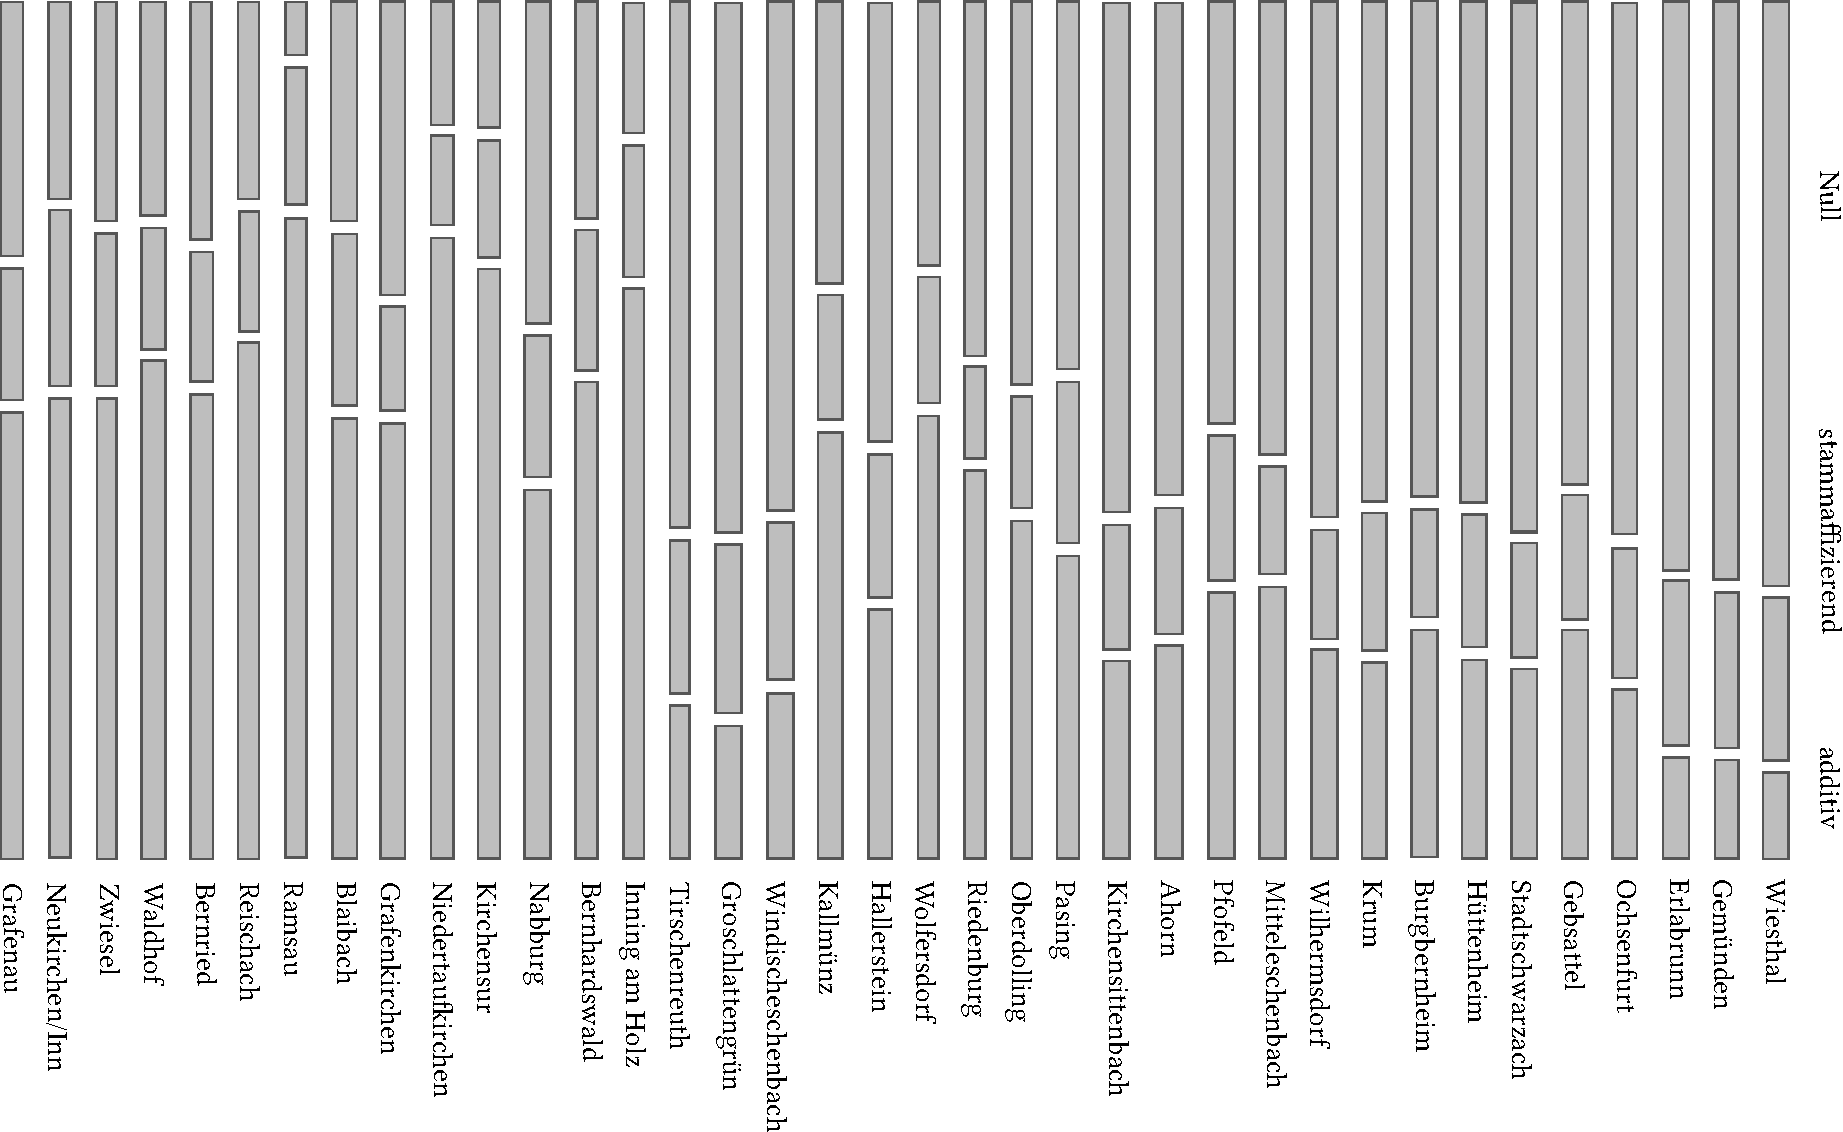
\includegraphics[height=.875\textwidth,angle=90]{figures/revisedNickelNominalmorphologie-img009a.pdf}
\caption{Feminina ($n=3.108$)}
\label{fig:3a}
\end{subfigure}
\caption{Mosaik-Plot der Häufigkeitsverteilung von additiver, stammaffizierender und Nullmarkierung bei den drei Genera (insgesamt $n=7.945$)}
\label{fig:3}
\end{figure}
\begin{figure}\ContinuedFloat
\begin{subfigure}{\textwidth}\centering
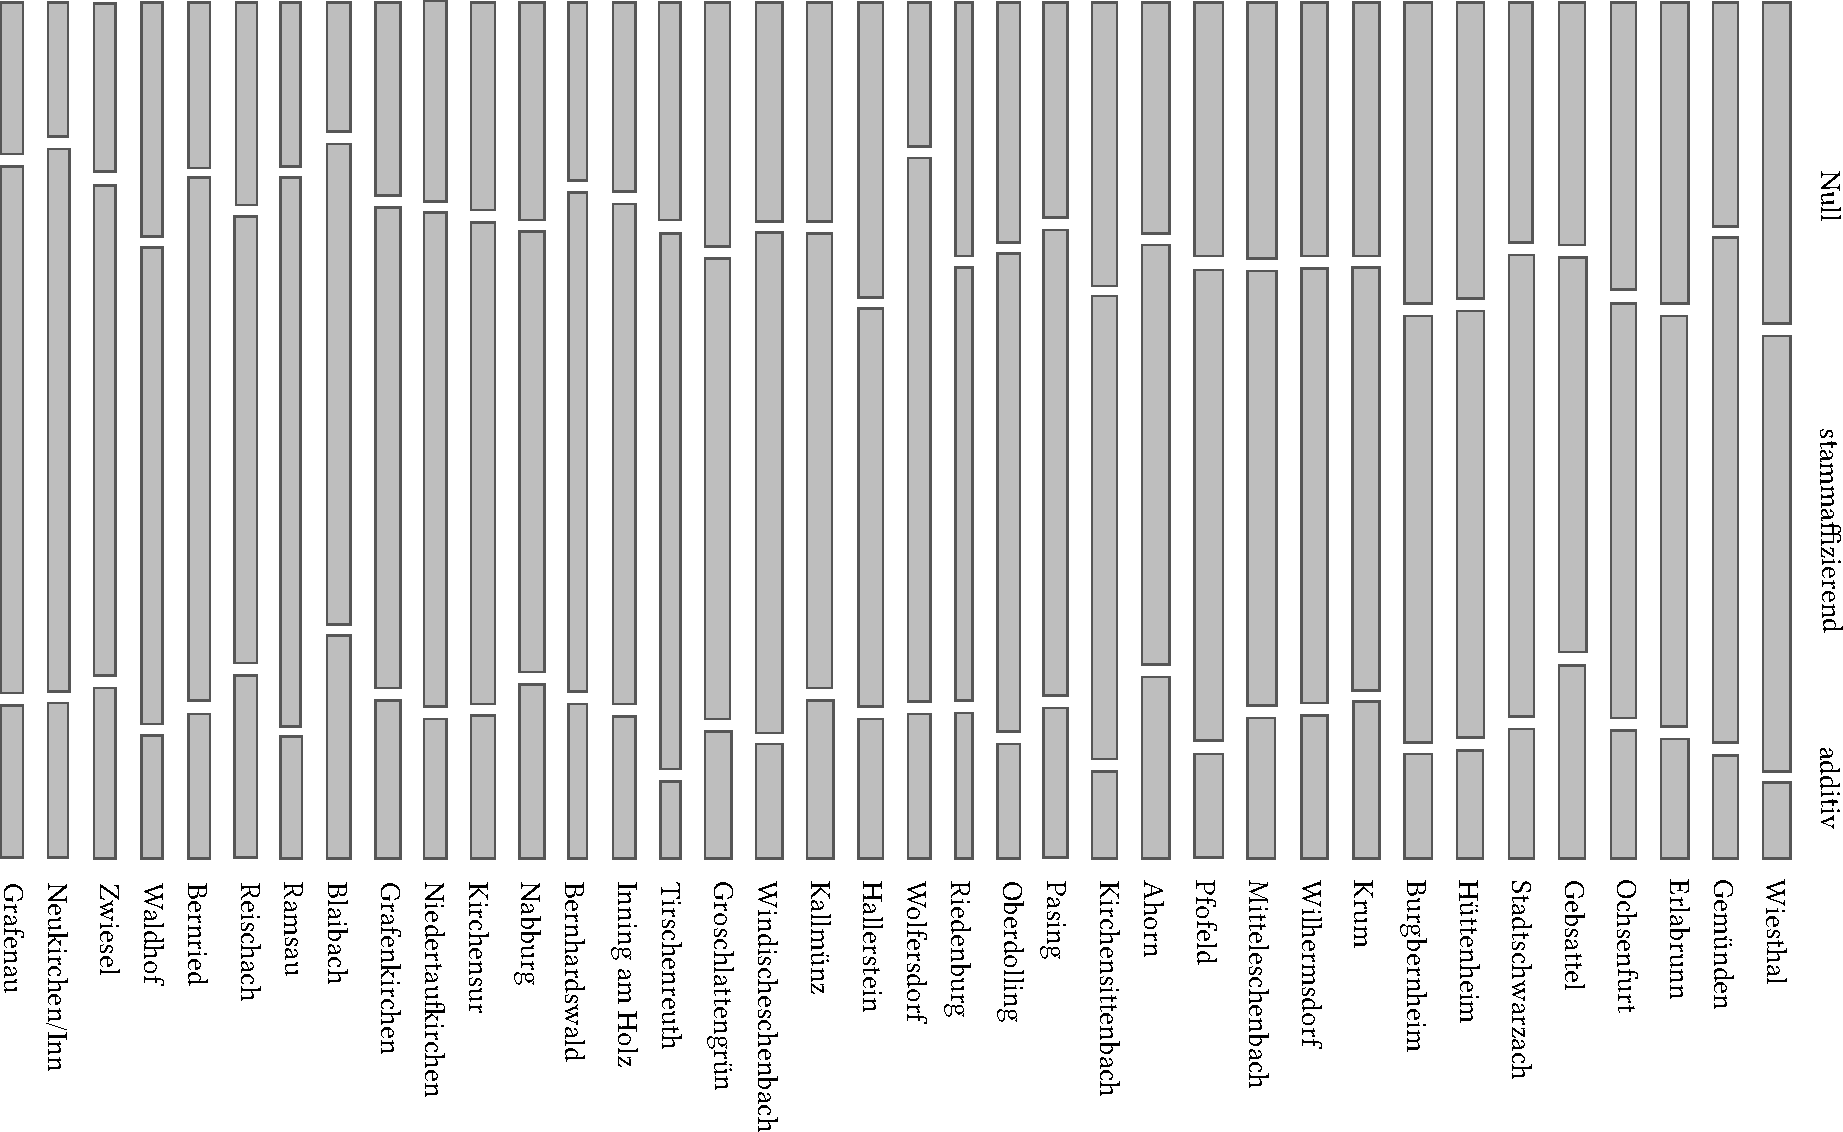
\includegraphics[height=.9\textwidth,angle=90]{figures/revisedNickelNominalmorphologie-img009b.pdf}
\caption{Maskulina ($n=3.426$)}
\label{fig:3b}
\end{subfigure}
\end{figure}
\begin{figure}\ContinuedFloat
\begin{subfigure}{\textwidth}\centering
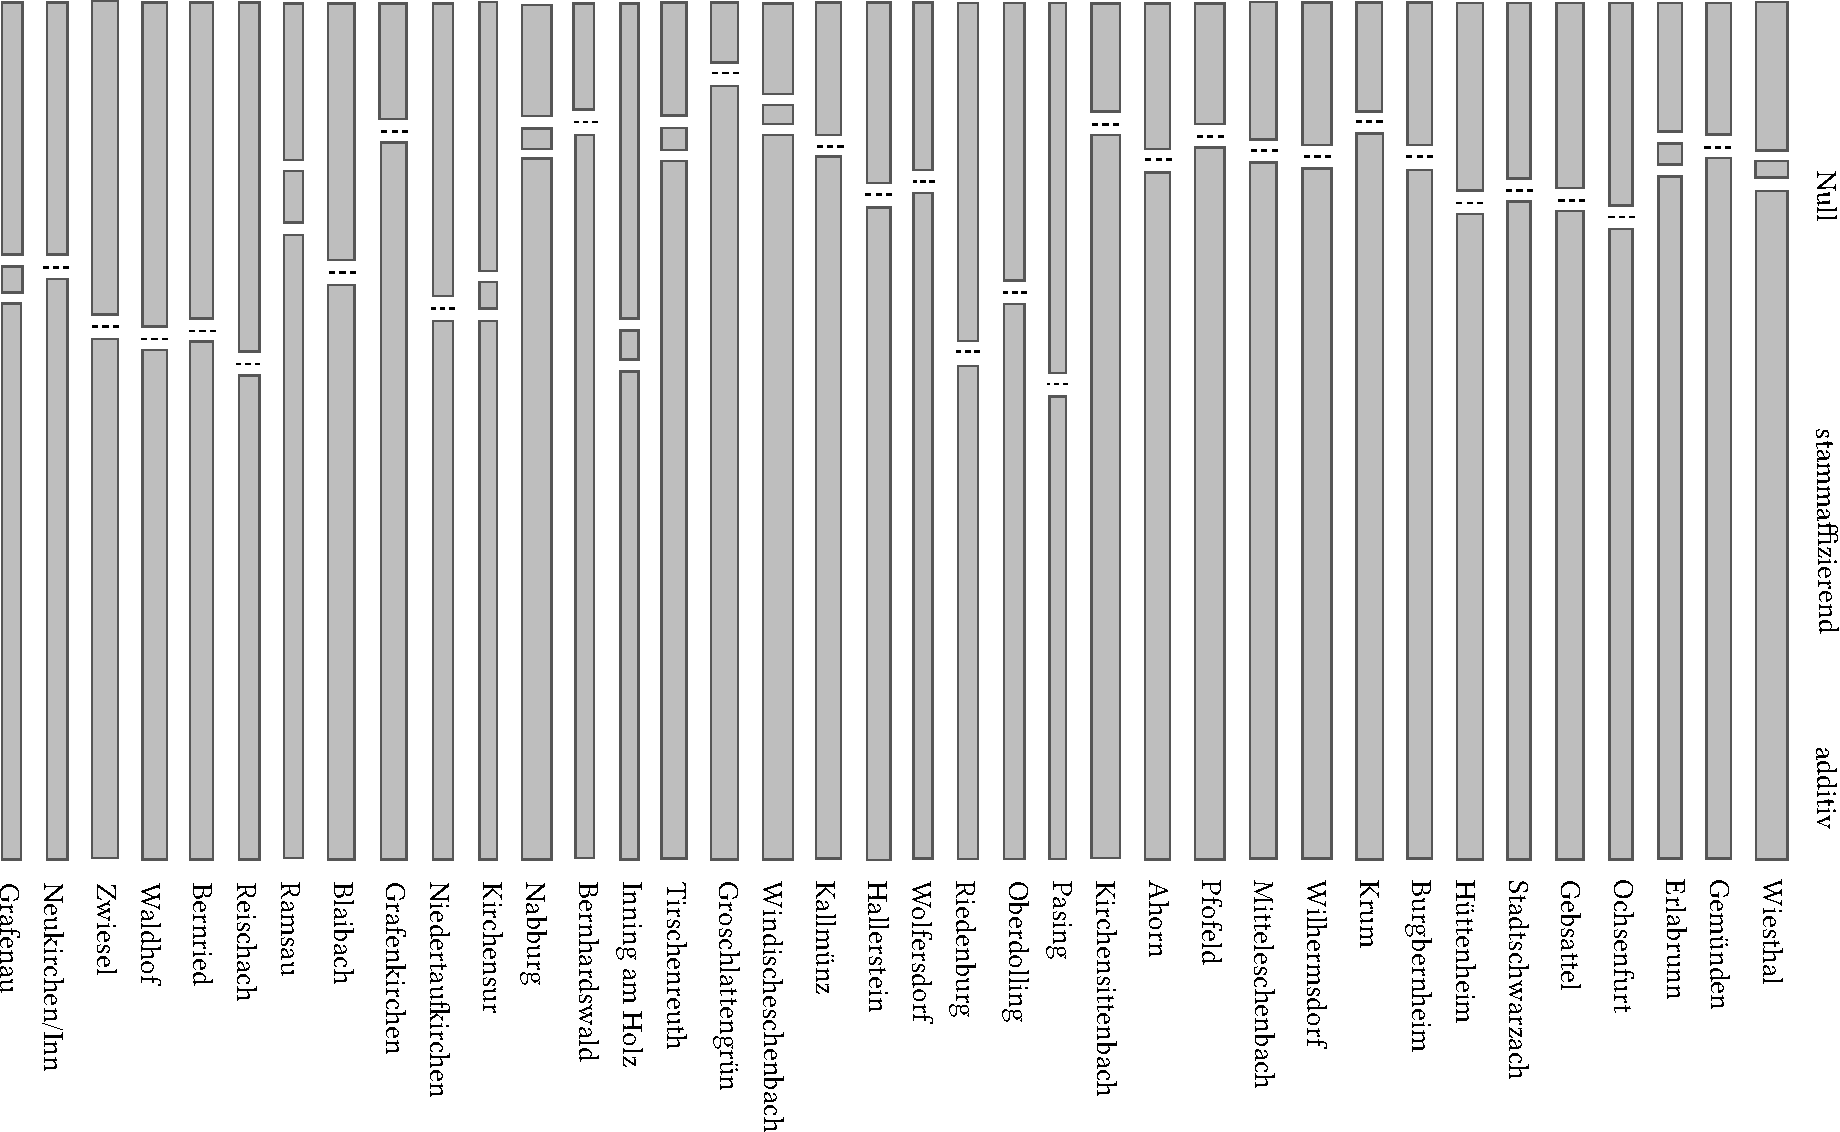
\includegraphics[height=.9\textwidth,angle=90]{figures/revisedNickelNominalmorphologie-img009c.pdf}
\caption{Neutra ($n=1.411$)}
\label{fig:3c}
\end{subfigure}
\end{figure}



\subsubsection{Inventar der Pluralsuffixe}
\label{sec:7.1.1.1}
Additive Pluralmarkierung ist durch Morphophonologie insofern bedingt, als das synchrone Inventar und die areale Verteilung der Flexionssuffixe das Ergebnis historischer phonologischer Prozesse ist (auf Basis der historischen Deklinationsklassenzugehörigkeit). Die phonologischen Prozesse, die im Bereich der Addition relevant sind, betreffen jeweils die Reduktionssilbe. Infolge der Schwa-Apokope entfällt ein additives Verfahren, die Suffigierung mit dem Schwa-Suffix (vgl. standardsprachlich \textit{Hund-e}). Daneben wird die Reduktionssilbe mhd. -\textit{en} in Teilen des UGs mit elidiertem finalen /n/ realisiert, d.\,h. hier besteht Varianz in der formalen Realisierung der Pluralsuffixe -\textit{en} und -\textit{n} (\textit{Ohr-en}, \textit{Hase-n}) in den rezenten Dialekten. Mit Blick auf diese beiden phonologischen Prozesse leiten sich aus einem kontrastiven Vergleich der Flexionssysteme im UG, zwischen dialektalem und standardsprachlichem System oder einer historischen Sprachstufe, zunächst zwei Fragenkomplexe ab:

\begin{itemize}
\item Wie setzt sich das Suffixinventar in Dialekten mit Schwa-Apokope vs. mit Schwa-Erhalt und jenen mit vs. ohne wortfinaler \textit{n}{}-Elision zusammen? Inwiefern variiert (in strukturalistischer Terminologie) der \textit{valeur} der einzelnen Suffixe, d.\,h. ihre Funktionalität und Distribution im jeweiligen Flexionssystem?
\item Lassen sich in apokopierenden Dialekten flexivische Verfahren identifizieren, die Numerussynkretismus infolge der Apokope des Schwa-Suffixes „kompensieren“, und wie sehen diese aus (vgl. \citealt[1197--1198]{Dingeldein1983}, \citealt[135]{Girnth2006}, \citealt[163--164]{Schirmunski1962})?
\end{itemize}

Im oobd. Sprachraum setzt dieApokope in der zweiten Hälfte des 13. Jahrhunderts ein. In Texten des Zeitraums zwischen 1300 und 1350 ist das Pluralsuffix -\textit{e} der alten mask. \textit{a}{}- und \textit{i}{}-Deklination im Bair. und im alem.-bair. Übergangsgebiet bereits zu 100\,\% apokopiert (\citealt[136]{KleinEtAl2018}). Die untersuchten Ortsdialekte des UG gehören zum obd. Apokopegebiet, wenngleich \citet[51 und 203]{Birkenes2014} zeigt, dass es problematisch ist, von rein apokopierenden vs. schwa-erhaltenden Dialekten auszugehen, da es zu wenige empirische Studien über den Status des Schwa in den deutschen Dialekten gibt; vielmehr handele es sich um Tendenzen, da die Apokope einen natürlichen phonologischen Prozess darstelle.

Die Zusammenschau der relevanten Wenker-Karten\footnote{Vgl. die Wenker-Karten zum Nominalbereich mit den Substantivformen des Nom.Pl. (108 „Füße“, 188 „Gänse“, 520 „Leute“, 406 „Berge“), des Dat.Sg. (373/374 „Hause“, 451 „Tische“, 524 „Felde“), die Singularformen mhd. schwacher Feminina (223 „Flasche“, 444 „Seife“, 550 „Wiese“) sowie die schwachen Adjektivformen (43 „gute“, 45 „alte“, 59 „kalte“, 319 „neue“, 531 „brauen“).} zeigt, dass die Untersuchungsorte trotz variierender Isoglossen jeweils im obd. Apokopegebiet liegen. Allerdings finden sich Pluralformen mit Schwa-Suffix für \textit{Gänse} und \textit{Berge} im ofr. Pfofeld (\textit{die bäsen Gänse} ‚die bösen Gänse‘), im ofr. Hallerstein (\textit{Uns’er Berge} ‚unsere Berge‘) und im ofr.-hess. Wiesthal (\textit{onr Berge}). Auf den ersten Blick lässt sich hier nicht sagen, ob es sich um standardnahe Formen handelt oder ob Schwa im dialektalen Suffixinventar auch im obd. Apokopegebiet anzusetzen ist. \mapref{map:3} illustriert, dass additive Formen mit Schwa-Suffix insbesondere im ofr. Teil des UGs durchaus zu finden sind, z.\,B. \teuthoo{hu.nd}{huͅnd} -- \teuthoo{hu.ndE}{huͅndə} ‚Hund‘ (ofr. Gebsattel). Dieses Schwa (und damit die gesamte Pluralform) gleicht in der rezenten Form der standardsprachlichen Form \textit{Hunde}, allerdings unterscheiden sich die Tiefenstrukturen: In der standardsprachlichen Form wird der Plural mit Schwa-Suffix markiert, während die dialektale Form auf die Form *\textit{hund-en} (und damit einen Deklinationsklassenwechsel) zurückgeht, in der das wortfinale /n/ getilgt wurde. Wortfinales Schwa ist in „geschützter Stellung“ \citep[203]{Birkenes2014} vor Nasal damit auch in apokopierenden Dialekten zu finden, vgl. die apokopierte Singularform und die Pluralform mit Schwa-Suffix im ofr. Gemünden am Main: \teuthoo{ho.2s5}{hōͅs̩} -- \teuthoo{ho.2sE}{hōͅsə} ‚Hase‘.

Die Realisierung des Nasalsuffixes mhd. \textit{en} erfolgt in den untersuchten Dialekten in Abhängigkeit von der phonologischen Umgebung. In einem breiten Streifen im Alemannischen und westlichen Ofr. („etwa bis Würzburg“, \citealt[387]{Schirmunski1962}) wird auslautender Nasal in Reduktionssilbe in allen phonologischen Umgebungen elidiert.\footnote{Vgl. \citet[46h]{Kranzmayer1956}, \citet[401]{Rowley1990a}, \citet[143]{Brenner1895} sowie \citet[68--69]{Kemmeter1924}, \citealt[Karte 120]{SBS9.1} und \citealt{WA}-Karte 546 „hinten“ zur Arealität in diesem Teil des Ofr.} Im übrigen Ofr. sowie im Nord- und Mittelbair. ist die Nasaltilgung durch den vorausgehenden Konsonanten bedingt.\footnote{Vgl. \citet[§95.2]{Gebhardt1907}, \citet[Karte 23]{Gütter1971}, \citet[§11]{Frommann1857}, \citet[42]{Hinderling1980}, \citet[Karte 24]{Kranzmayer1956}, \citet[425]{Rowley1990b}, \citet[76--77 und Karte 19]{Rowley1997}, \citet[§582--585]{Schmeller1821}, \citealt{WA}-Karte 444 „Seife“, \citet[101--104]{Wildfeuer2001}.} 	\tabref{tab:16} zeigt anhand exemplarischer Ortsdialekte, dass die vokalische Realisierung von -\textit{en} nach Nasal im gesamten UG erfolgt und gebietsweise nach Stammvokal (Langvokal oder Diphthong),\footnote{Im Datenmaterial ist nur das zweisilbige \textit{Klaue} belegt, das im Ofr. (inklusive ofr.-nordbair. Übergangsgebiet) mit vokalischem Suffix realisiert wird (z.\,B. \teuthoo{gla4<o4u\^A94}{ɡlậọü̯α\klammeruntenpost{}̣} -- \teuthoo{gla4<o4u\^A94}{ɡlậọü̯α\klammeruntenpost{}̣} im ofr. Wilhermsdorf). Im Nord- und Mittelbair. finden sich vor allem nicht-suffigierte Formen im Singular und Plural, daneben vereinzelte Formen mit Nasal (\teuthoo{glôo.<u}{ɡl{\aufstrih}ôͅu} -- \teuthoo{glôo.<un}{ɡl{\aufstrih}ôͅun} im nordbair. Oberdolling) und vokalischem Suffix (\teuthoo{gðlôo4<{gðlôo4<\&ûu.<e4}ûu.<e4}{ɡ̩l{\aufstrih}ộ̃̃{\aufstrih}ûͅẹ} -- \teuthoo{gðlôo4<{gðlôo4<\&ûu.e4n}ûu.e4n}{ɡ̩l{\aufstrih}ộ̃̃{\aufstrih}uͅẹn} im mittelbair. Reischach).} im südlichen Nordbair. und im Mittelbair. zudem nach mhd. \textit{ch}, \textit{f}, \textit{ff}, \textit{pf}, \textit{k}. Nach mhd. \textit{gg} in \textit{Brücke}, \textit{Mücke}, \textit{Glocke}, nach Dental sowie nach den bilabialen Plosiven /p/, /b/ wird -\textit{en} dagegen als Nasal realisiert (ausgenommen ist hier der Vokalisierungsstreifen im westlichen Ofr.).


\begin{table}
\small
\begin{tabularx}{\textwidth}{QQQQQQ}
\lsptoprule
& {Tanne}

 (mhd. \textit{n}) & {Seife}

 (mhd. \textit{f}) & {Eiche}

 (mhd. \textit{(c)h}) & {Stecken}

 (mhd. \textit{k}) & {Karpfen/}

{ Schupfen}

 (mhd. \textit{pf})\\
 \midrule
westl. Ofr.

(Erlabrunn) & \teuthoo{da.nA}{daͅnα} -- \teuthoo{da.nA}{daͅnα} & Sg. \teuthoo{se.v5A94}{seͅv̩α\klammeruntenpost{}̣} & \teuthoo{e.cE}{eͅXə} -- \teuthoo{e.cE}{eͅXə} & Sg. \teuthoo{A4n}{α̣n} \teuthoo{s\#da4gA)4}{šdạɡα\klammeruntenpost{}̣} & {\teuthoo{kharbv5E}{kharbv̩ə} --}

 \teuthoo{kharbv5E}{kharbv̩ə}

\teuthoo{s\#u.bE}{šuͅbə} -- \teuthoo{s\#u.bE}{šuͅbə}\\
\tablevspace
Ofr.

(Wilherms\-dorf) & \teuthoo{da.nA94}{daͅnα\klammeruntenpost{}̣} -- \teuthoo{da.nA94}{daͅnα\klammeruntenpost{}̣} & \teuthoo{sa42v5m}{sạ̄v̩m} -- \teuthoo{sa42v5m}{sạ̄v̩m} & \teuthoo{a94xY}{a\klammeruntenpost{}̣x{\klammerNG}} -- \teuthoo{a94xY}{a\klammeruntenpost{}̣x{\klammerNG}} & \teuthoo{s\#de9.gY}{šde\klammeruntenpost{}ͅɡ{\klammerNG}} -- \teuthoo{s\#de9.gY}{šde\klammeruntenpost{}ͅɡ{\klammerNG}} & {\teuthoo{k\_a.rbv5m}{kʰaͅrbv̩m} --}

 \teuthoo{k\_a.rbv5m}{kʰaͅrbv̩m}\\
 \tablevspace
nördl. Nordbair.

(Grosch\-latten\-grün) & \teuthoo{d5å"nA}{d̩{\burgeroalphamakron}nα} -- \teuthoo{d5å"nA}{d̩{\burgeroalphamakron}nα} & \teuthoo{so9.i.fm@}{so\klammeruntenpost{}ͅiͅfm̥} -- \teuthoo{so9.i.fm@}{so\klammeruntenpost{}ͅiͅfm̥} & \teuthoo{qo.<i.cN@}{ʔôͅiͅXŋ̥} -- \teuthoo{qo.<i.cN@}{ʔôͅiͅXŋ̥} & \teuthoo{s\#de.kqN@}{šdeͅkʔŋ̥} -- \teuthoo{s\#de.kqN@}{šdeͅkʔŋ̥} & {\teuthoo{g\_o3Apfm@}{ɡʰŏαpfm̥} --}

 \teuthoo{g\_o3Apfm@}{ɡʰŏαpfm̥}

\teuthoo{s\#upfm@}{šupfm̥} -- \teuthoo{s\#upfm@}{šupfm̥}\\
\tablevspace
südl. Nordbair./

nordbair.-mittelbair. Übergangs\-gebiet

(Kallmünz) & \teuthoo{da.nA}{daͅnα} -- \teuthoo{da.nAn}{daͅnαn} & \teuthoo{so.ifA}{soͅifα} -- \teuthoo{so.ifAn}{soͅifαn} & \teuthoo{o.iX!A}{oͅiꭖα}-- \teuthoo{o.ic1An}{oͅiX\⚬αn} & {\teuthoo{s\#de.kA}{šdeͅkα} --}

 \teuthoo{s\#de.kAn}{šdeͅkαn} & {\teuthoo{k,\_a.rpfA}{k͓ʰaͅrpfα} --}

 \teuthoo{k\_arpfAn}{kʰarpfαn}

\teuthoo{s\#u.pfA}{šuͅpfα}-- \teuthoo{s\#u.pfAn}{šuͅpfαn}\\
\tablevspace
Mittelbair.

(Grafenau) & {\teuthoo{A}{α} \teuthoo{d5e."+nA}{d̩ẽ̄ͅnα} --}

 \teuthoo{de.>+nAn}{dễͅnαn}, \teuthoo{de.>+nAne4}{dễͅnαnẹ} & {\teuthoo{s5o.<Af,E}{s̩ôͅαf͓ə} --}

 \teuthoo{s\%o.<AfEn}{s͈ôͅαfən} & {\teuthoo{o9.<AxA}{o\klammeruntenpost{}̂ͅαxα} --}

 \teuthoo{o9.<AxAn}{o\klammeruntenpost{}̂ͅαxαn} & Sg. \teuthoo{s\#5d5ekA}{š̩d̩ekα} & {\teuthoo{s\#u.b\%v\%A}{šuͅb͈v͈α} --}

 \teuthoo{d5s\#5u.pfAn}{d̩š̩uͅpfαn}\\
 \tablevspace
mittelbair-südbair. Übergangsgebiet (Ramsau) & \teuthoo{d\%a.<n}{d͈âͅn} -- \teuthoo{d\%a.nA}{d͈aͅnα} & \teuthoo{s\%oAfð5}{s͈oαf̩̩} -- \teuthoo{s\%oa4fn@}{s͈oạfn̥} & \teuthoo{o4a4X!}{ọạꭖ} -- \teuthoo{o4a4X!Y@}{ọạꭖ{\klammerNG}̥} & Sg. \teuthoo{s\#\%t,e.kHEY}{š͈t͓eͅkhͯə{\klammerNG}} & {}--\\
\lspbottomrule
\end{tabularx}
\caption{Realisierung der Reduktionssilbe -\textit{en} in standardsprachlichen Zweisilbern in der Singular- und Pluralform (sofern in den Daten belegt) in exemplarischen Ortspunkten des UG (vgl. Karte 19 in \citealt{Rowley1997})}
\label{tab:16}
\end{table}

An den verschiedenen Formen in 	\tabref{tab:16} fällt auf, dass die Qualität des reduzierten Vokals im UG und auch in den Ortsdialekten variiert (vgl. \citealt[387]{Schirmunski1962}). Die areale Verteilung der vokalischen Pluralsuffixe in \mapref{map:3} illustriert, dass in den ofr. Ortsdialekten vor allem -\textit{\teuthoo{E}{ə}} und -\textit{\teuthoo{E.}{əͅ}} (für den Reduktionsvokal zwischen [\teuthoo{A}{α}] und [\teuthoo{E}{ə}]) belegt ist, während im bair. Teil des UGs (inklusive ofr.-nordbair. Übergangsgebiet) vor allem -\textit{\teuthoo{A}{α}} („Tiefschwa“) und in geringerem Maße -\textit{\teuthoo{E}{ə}} erscheint (vgl. \citealt[6]{Mausser1915}).\footnote{Daneben findet sich in den bair. Ortsdialekten teilweise Vollvokal (vgl. \teuthoo{mo.<Ak}{môͅαk} -- \teuthoo{me.<k,t,e4}{mêͅk͓t͓ẹ} ‚Markt‘ im mittelbair. Reischach und \teuthoo{s\#ta42l}{štạ̄l} -- \teuthoo{s\#ta4<l"e4}{štậl̄ẹ} ‚Starl‘ im mittelbair. Wolfersdorf mit vorderem [\teuthoo{e.}{eͅ}] und \teuthoo{nuS}{nuʃ} -- \teuthoo{ni.ʃ{\textasciitilde}ôe.}{niʃ{\aufstrih}e} ‚Nuss‘ im nordbair. Groschlattengrün mit zentralisiertem [\teuthoo{e.}{eͅ}]).}  Die Durchsicht der Belege zeigt, dass die Distribution der vokalischen Suffixe in jenen Orten, die verschiedene Abstufungen des Reduktionsvokals oder vereinzelt Vollvokal aufweisen, durch phonetische Variation bedingt ist: Schwa und Tiefschwa erscheinen in den gleichen Kontexten (vgl. \citealt[15]{Köhler1934}). Es ist hier also sinnvoll, phonetische Varianz auf einem Kontinuum zwischen \textit{e}{}- und \textit{a}{}-Färbung anzunehmen, zumal das ausdifferenzierte Notationssystem der Teuthonista diese Abstufungen wiedergibt und hier auch Transkriptionseffekte zu beobachten sind.\footnote{Beispielsweise im ofr. Gebsattel, wo die Singular- und Pluralform von ‚Ratte‘ mit differenter Reduktionssilbe transkribiert ist (\teuthoo{ra94dE.}{ra\klammeruntenpost{}̣dəͅ} -- \teuthoo{ra94dA}{ra\klammeruntenpost{}̣dα}), die Gewährsperson aber angemerkt hat „Sg. + Pl. klingt gleich“.}

Dennoch erscheint es -- zumindest im Rahmen einer ersten Klassifikation -- nicht praktikabel, Schwa und Tiefschwa zu einem einzigen vokalischen Suffix zusammenzufassen. Zum einen gibt es Hinweise in der Literatur, dass -\textit{α} und -\textit{ə} im Ofr. phonologisch distinkt sind (vgl. \citealt[82]{Rowley1997}). So findet sich laut \citet[214--215]{Diegritz1971} im Osten Mittelfrankens eine Opposition zwischen /ɐ/ als synchroner Entsprechung von mhd.-\textit{e}/-\textit{en} und /ə/ für mhd. -\textit{er}/-\textit{ære}, während im westlichen Mittelfranken die Opposition zwischen /ə/ (mhd. -\textit{en}, -\textit{em}, -\textit{e}) und /r/ (mhd. -\textit{er}, {}-\textit{ære}) besteht. In dieser Eindeutigkeit können die Verhältnisse für die ofr. Daten allerdings nicht bestätigt werden. Anderseits gibt es Dialekte -- und hier lohnt ein Blick jenseits des eigenen UGs in das Schwäb. und das mittelbair.-schwäb. Übergangsgebiet --, in denen -\textit{α} und -\textit{ə} tatsächlich phonologisch distinkt sind. In einem kleinen Areal im südlichen SBS-Arbeitsgebiet alterniert das Stammsuffix der mhd. schwachen Feminina zwischen -\textit{ə} im Singular und -\textit{α} im Plural: \teuthoo{A}{α} \teuthoo{nu.<iE@}{nûͅiə̥} \teuthoo{glo4kE}{ɡlọkə} -- \teuthoo{nu.<iE@}{nûͅiə̥} \teuthoo{glo4ka}{ɡlọka} ‚eine neue Glocke/neue Glocken‘ (schwäb. Bernbeuren, vgl. \mapref{map:33}, \sectref{sec:7.1.1.4} sowie \citealt[Karten 105--117]{SBS9.1}, \citealt[8]{Rowley1994}).

\begin{sloppypar}
Für das gesamte Untersuchungsgebiet können folgende Suffixtypen unterschieden werden, das (orts-)dialektspezifische Inventar und die areale Variation der Suffixe ergeben sich jeweils aus dem phonologischen System respektive aus den historischen phonologischen Prozessen:\footnote{Daneben findet sich ein einzelner Beleg für \textit{s}{}-Suffix: Die Gewährsperson in Krum bildet die Pluralform zu ‚Kummet‘ spontan als \teuthoo{khumEds}{khuməds} und bietet anschließend die Form \teuthoo{khumEdn}{khumədn} mit dem Kommentar „besser“. Das \textit{s}-Suffix wird im Folgenden daher nicht weiter berücksichtigt (vgl. \sectref{sec:4.2.1} und \citealt[1199]{Dingeldein1983} zum \textit{s}-Suffix in den deutschen Dialekten).} 
\end{sloppypar}

\begin{itemize}
\item \textit{Nasalsuffix} in den phonetischen Realisierungen [m], [n], [ŋ]: Nach (bi-)""labialem Plosiv oder Frikativ wird das Nasalsuffix zu [m] assimiliert, nach velarem Plosiv zu [ŋ] (vgl. \citealt[Karte 24]{Kranzmayer1956}, \citealt[126 und Karte 220]{Rowley1997}, \citealt[388]{Schirmunski1962}, \citealt[§578--580]{Schmeller1821}).\footnote{Vgl. \citet[57--58]{Kufner1961}, \citet[121]{Steininger1994} zum Mittelbair. sowie \citet[§45.I]{Hain1936}, \citet[67--68]{Kemmeter1924}, \citet[15]{Köhler1934} zum Ofr.} Daneben erfolgt gebietsweise Elision des stammauslautenden Konsonanten \textit{b} (\textit{w}), \textit{d}/\textit{t}, \textit{g}, \textit{r} und \textit{x} vor Nasalsuffix, z.\,B. \teuthoo{gða.rb}{ɡ̩aͅrb} -- \teuthoo{gða.rm}{ɡ̩aͅrm} ‚Garbe‘ (mittelbair. Kirchensur), \teuthoo{saux}{saux} -- \teuthoo{tauN}{tauŋ} ‚Auge‘ (nordbair. Nabburg, vgl. \citealt{Rowley1997}: 126).

Im bair. Teil des UGs wird Nasalsuffix teilweise als Reduktionssilbe mit Tiefschwa [αn] realisiert, vgl. \teuthoo{bre4m}{brẹm} -- \teuthoo{bre4"(+mAn}{brẹ̃̄\klammerobenpost{}mαn} ‚Bremse‘ (mittelbair. Niedertaufkirchen), \teuthoo{le.Ax5}{leͅαx̩} -- \teuthoo{le.<AhA4n}{lêͅαhα̣n} ‚Lärche‘ (mittelbair. Waldhof). Diese Realisierungsform findet sich nur bei historisch zweisilbigen Feminina mit apokopierter Singularform. \citet[§26]{Micko-Repp1933} zufolge handelt es sich um eine Neubildung: An das Suffix -\textit{α}, das lautgesetzlich nach Nasal oder Velarplosiv/-frikativ im Stammauslaut erscheint, wird das Nasalsuffix -\textit{n} gehängt, sodass hier eine Art Doppelsuffigierung entsteht (vgl. \citealt[§49]{Kollmer1985}, \citealt[153]{Rowley1997}). Die Outputstruktur der Pluralform entspricht in der Folge den Pluralformen mit Nasalsuffix der \textit{n}{}-erweiterten Feminina mit vokalisch realisierter Reduktionssilbe: \teuthoo{bre42mA}{brẹ̄mα} -- \teuthoo{bre42mAn}{brẹ̄mαn} ‚Bremse‘ (mittelbair. Pasing), \teuthoo{le.AXA}{leͅαꭗα} -- \teuthoo{le.AXAn}{leͅαꭗαn} ‚Lärche‘ (nordbair.-mittelbair. Zwiesel, siehe hierzu ausführlicher Abschnitte~\ref{sec:7.1.1.3} und \ref{sec:8.3.3.1})

\item \textit{\textit{(ə)r}{}-Suffix}
\item \textit{\textit{α}}\textit{{}-Suffix} als vokalische Realisierung von mhd. -\textit{er}, mhd. -\textit{en}
\item \textit{\textit{ə}}\textit{{}-Suffix} als vokalische Realisierung von mhd. -\textit{er}, mhd. -\textit{en}
\end{itemize}

Die oben beobachtete Zweiteilung des UGs in ein bair. vs. ofr. Gebiet setzt sich in der arealen Distribution der Suffixe und in der ortsdialektspezifischen Zusammensetzung des Suffixinventars fort. Im bair. Teil (inklusive nordbair.-ofr. Übergangsgebiet) findet sich ein -- im historischen wie interdialektalen Vergleich -- reduziertes Inventar mit Nasal- und \textit{α}{}-Suffix (daneben teilweise Schwa-Suffix). Neben dem Pluralsuffix mhd. -\textit{en} in bestimmten phonologischen Umgebungen wird auch die Reduktionssilbe mhd. -\textit{er} im bair. Teil des UG vokalisiert als -\textit{α} realisiert, weshalb das \textit{α}{}-Suffix in diesen Dialekten (mit Bezug auf das standardsprachliche System oder eine historische Sprachstufe) „tiefenstrukturell mehrdeutig“ \citep[127]{Rowley1997} ist.\footnote{Vgl. \citet[113]{Haas1983}, \citet[§50c3 und Karte 26]{Kranzmayer1956}, \citet[65]{RennKönig2006}, \citet[82 und Karte 19]{Rowley1997}, \citet[257 und Karte 9]{Werner1961} sowie die \citealt{WA}-Karten 4 „Winter“, 61 „Wasser“, 105 „Pfeffer“.} Das Suffixsystem dieses Typs unterscheidet sich von Systemen, in denen mhd. -\textit{er} und mhd. -\textit{en} auch synchron unterschieden sind, etwa in einem Teil des Unterofr., wo die Reduktionssilbe mhd. -\textit{er} als konsonantisches [r] und mhd. -\textit{en} vokalisch realisiert wird. In den übrigen ofr. Tiefenbohrungspunkten besteht Variation in der spezifischen Verteilung konsonantischer und vokalischer Pluralsuffixe in Abhängigkeit von den phonologischen Systemen. Im ofr. Stadtschwarzach und Hüttenheim beispielsweise werden mhd. -\textit{er} und -\textit{en} konsonantisch realisiert, nur nach Nasal und Stammvokal erfolgt Elision des wortfinalen /n/, sodass die Distribution von Nasal- und (Tief-)Schwa-Suffix hier phonotaktisch konditioniert ist (vgl. \sectref{sec:8.3.3.2}). In den übrigen Orten erscheinen sowohl vokalische als auch konsonantische Realisierung von mhd. -\textit{er} und -\textit{en}. Schwa und Tiefschwa sind auch hier „tiefenstrukturell mehrdeutig“, da sie vokalische Realisierungen von mhd. -\textit{er} und -\textit{en} repräsentieren.

Die methodische Schwierigkeit der Analyse besteht nun darin, die Distribution der vokalischen Suffixe auf der phonetischen und auf der morphophonologischen Ebene adäquat abzubilden (vgl. \citealt[40--43]{Hinderling1980}, \citealt[126--129]{Rowley1997}, \citealt[29--30]{SMF7}). Eine Möglichkeit der Analyse besteht darin, die jeweiligen konsonantischen und vokalischen Realisierungen als eigene Suffixtypen zu klassifizieren und damit v.\,a. die synchrone Perspektive zu berücksichtigen (vgl. z.\,B. \citealt[38]{Gladiator1971} und \citealt[57--60]{Kufner1961}). Demnach würden die Suffixe der Flexionsformen von \textit{Hase} im westlichen Ofr. der phonetischen Realisierung entsprechend als drei verschiedene Flexionssuffixe -\textit{ən}, -\textit{ə}, -\textit{α} klassifiziert, vgl. Nom.Sg. \teuthoo{ho9.2s5}{ho\klammeruntenpost{}̄ͅs̩} -- Akk.Sg. \teuthoo{ho9.2sn@}{ho\klammeruntenpost{}̄ͅsn̥} -- Nom.Pl. \teuthoo{ho9.2sn@}{ho\klammeruntenpost{}̄ͅsn̥} (ofr. Burgbernheim), \teuthoo{ho.2s5}{hōͅs̩} -- \teuthoo{ho.2sE}{hōͅsə} --\teuthoo{ho.2sE}{hōͅsə} (ofr. Gebsattel), \teuthoo{ha.2s5}{hāͅs̩} -- \teuthoo{An}{αn} \teuthoo{ha2.sA}{hāͅsα} -- \teuthoo{ha:2sA}{ha{\doubleogonek}̄sα} (ofr. Erlabrunn).\footnote{\citet[38]{Gladiator1971} analysiert das \textit{α}{}-Suffix als Allophon des Phonems /a/ gegenüber den Suffixen [m, n, ŋ] als Allophon von /-n/, da /a/ und /-n/ im Wortauslaut in Opposition stehen könnten, z.\,B. /hɔasa/ ‚heißer‘ vs. /hɔasn/ ‚heißen‘. In dieser Lösung wird die „tiefenstrukturelle“ Mehrdeutigkeit \citep[127]{Rowley1997} der Flexive -\textit{er} und -\textit{en} nicht aufgelöst, \textit{α}{}- und Nasalsuffix werden rein synchron klassifiziert. Anders geht \citet[§27]{Micko-Repp1933} vor, die das \textit{α}{}-Suffix auf -\textit{er} zurückführt, das von den Neutra auf Feminina und Maskulina übertragen wurde.}

Eine alternative Form der Analyse besteht in der Klassifikation von -\textit{ən}, -\textit{ə}, \mbox{-\textit{α}} als Heteromorphe des Nasalsuffixes, deren Distribution durch phonologische Faktoren dialektspezifisch gesteuert ist. Diese Form der Klassifikation ist hier naheliegend, da sich aus Obliquus- und Pluralform die Zuweisung zur schwachen Deklination ergibt. Eine eindeutige Klassifikation von Schwa und Tiefschwa als rezenter Entsprechung des Nasal- oder \textit{er}{}-Suffixes ist allerdings nicht in allen Fällen möglich, wie beispielsweise Pluralformen des Typs \teuthoo{ba2mA}{bāmα} ‚Baum‘ im Nordbair. zeigen (vgl. \citealt[128]{Rowley1997}). Mhd. -\textit{er} und mhd. -\textit{en} in der phonologischen Umgebung nach Nasal werden in diesem Gebiet jeweils als [α] realisiert. Daneben ist im Übergangsgebiet von zentralem und westlichem SMF-Untersuchungsgebiet Tiefschwa als Pluralmarker von \textit{Fleck} nicht eindeutig als Entsprechung von -\textit{er} oder -\textit{en} zu klassifizieren, da in diesem Areal beide Formen belegt sind (\citealt[29--30]{SMF7}). Zudem bleibt bei der zweiten Lösungsvariante offen, inwiefern -\textit{α} als rezente Entsprechung von -\textit{er} und -\textit{en} oder tatsächlich als eigenständiges Pluralsuffix mental repräsentiert ist. \citet[129]{Kalau1984} berichtet beispielsweise von der Verwechselung der standardsprachlichen Pluralsuffixe -\textit{er} und -\textit{en} bei Sprechern des Nürnberger Dialekts, wo beide Suffixe als -\textit{α} realisiert werden. Da es Ziel der synchronen Analyse ist, die Faktoren der Distribution der einzelnen Suffixe auf der Ebene des Einzeldialekts zu erarbeiten, wird auf eine abstrahierende Klassifikation zunächst verzichtet. Die Annotation der Suffixe erfolgte daher entsprechend ihrer phonetischen Realisierung.

\subsubsection{Kombinierte Verfahren}
\label{sec:7.1.1.2}
Neben rein additiven Pluralformen tritt das Pluralsuffix in Kombination mit einem oder mehreren stammaffizierenden Pluralmarkierungsverfahren auf (\tabref{tab:17}).


\begin{table}
\begin{tabularx}{\textwidth}{>{\raggedright\arraybackslash}p{.2\textwidth}lQ}
\lsptoprule

\multicolumn{3}{l}{Kombiniertes Verfahren aus Addition und \ldots}\\
\midrule
\multirow[t]{2}{=}{Kontrasten der Vokalqualität} & Umlaut & \teuthoo{s\#du.2m}{šdūͅm} -- \teuthoo{ds\#di“mA}{dšdīmα} ‚Stube‘ (nordbair.-mittelbair. Bernhardswald)\\
& mhd. \textit{ei} & \teuthoo{o2A}{ōα} -- \teuthoo{qo.<i.A}{ʔôͅiͅα} ‚Ei‘ (nordbair. Groschlattengrün)\\
\tablevspace
\multicolumn{2}{p{.4\textwidth}}{Kontrasten der Vokalquantität} & \teuthoo{no2l}{nōl} -- \teuthoo{noln}{noln} ‚Nadel‘ (mittelbair. Grafenau)\\
\tablevspace
\multicolumn{2}{>{\raggedright\arraybackslash}p{.4\textwidth}}{Umlaut + Kontrasten der Vokalquantität} & \teuthoo{ro42d}{rọ̄d} -- \teuthoo{re.3dA}{rĕͅdα} ‚Rad‘ (ofr. Pfofeld)\\
\tablevspace
\multirow[t]{2}{=}{Konsonantismus\-kontrasten} & Elision & \teuthoo{v5i“}{v̩ī} -- \teuthoo{v5i“cE}{v̩īXə} ‚Vieh‘ (ofr. Krum)\\
& \makecell[tl]{Lenis-Fortis-\\Kontraste} & \teuthoo{ho.ds}{hoͅds} -- \teuthoo{hôoi4tSA}{h{\aufstrih}oịtʃα} ‚Holz‘ (nordbair.-mittelbair. Blaibach)\\
\tablevspace
\multicolumn{2}{p{.4\textwidth}}{Lenis-Fortis-Kontrasten + Quantitätskontrasten} & \teuthoo{ne42sd}{nẹ̄sd} -- \teuthoo{ne4StA}{nẹʃtα} ‚Nest‘ (nordbair.-mittelbair. Zwiesel)\\
\tablevspace
\multicolumn{2}{p{.4\textwidth}}{Lenis-Fortis-Kontrasten + Quantitätskontrasten + Umlaut} & \teuthoo{vo2s}{vōs} -- \teuthoo{va4SA}{vạʃα} ‚Fass‘ (nordbair. Nabburg)\\
\lspbottomrule
\end{tabularx}
\caption{Übersicht kombinierter Pluralmarkierungsstrategien}
\label{tab:17}
\end{table}

Die einzelnen stammaffizierenden Verfahren werden in \sectref{sec:7.1.2}, deklinationsklassenspezifische Faktoren der Distribution in \sectref{sec:8.3} dargestellt.

\subsubsection{„Doppelsuffigierung“: -\textit{α} und -\textit{αn} im Bair.}
\label{sec:7.1.1.3}
Eine dialektraumspezifische Form additiver Pluralmarkierung findet sich im bair. Teil des UGs bei historisch zweisilbigen Feminina mit Schwa-Reduktionssilbe, die in der Singularform Nasalsuffix aufweisen (Typ \textit{Glocke-n}), das in Abhängigkeit von der phonologischen Umgebung des vorausgehenden Lauts als -\textit{n} oder vokalisch als -\textit{α} realisiert wird (vgl. \sectref{sec:7.1.1.1} und 	\tabref{tab:16}). Je nach konsonantischer oder vokalischer Realisierung der Reduktionssilbe erfolgt die additive Pluralmarkierung durch Nasal- oder Tiefschwa-Suffix, z.\,B. \teuthoo{biEkA}{biəkα} -- \teuthoo{biEkAn}{biəkαn} ‚Birke‘ (nordbair. Nabburg), \teuthoo{glok-N}{ɡlok{}͐ŋ} -- \teuthoo{glok-nA}{ɡlok{}͐nα} ‚Glocke‘ (mittelbair. Grafenau), sodass eine Art Doppelsuffigierung aus Stammbildungssuffix\footnote{Da es im Dialektvergleich und lexemweise auch im Ortsdialekt Variation zwischen Singularformen mit apokopierter Schwa-Reduktionssilbe und \textit{n}{}-Erweiterung gibt (z.\,B. \teuthoo{s\#dro2S}{šdrōʃ} neben \teuthoo{s\#dro2Sn}{šdrōʃn} ‚Straße‘, eingehender zur Problematik siehe Abschnitte~\ref{sec:7.1.3.1} und \ref{sec:8.2.3}), wird im Folgenden tatsächlich von einem Stammbildungssuffix ausgegangen. Allerdings ist nicht auszuschließen, dass nicht zumindest lexemweise eine Verschiebung der Morphemgrenze stattgefunden hat und die Reduktionssilbe als Teil des Stammes analysiert und abgespeichert wird. Dies scheint insbesondere dann plausibel, wenn eine Assimilation von Stammauslaut und Nasalsuffix vorliegt, etwa in \teuthoo{s\#tum}{štum} ‚Stube‘. Durch die dialektvergleichende Ausrichtung der Untersuchung und das Nebeneinander von apokopierten und \textit{n}{}-erweiterten Formen scheint das Konzept des Stammbildungssuffixes hier aber praktikabler.} der Singularform und Pluralsuffix -\textit{n} bzw. -\textit{α} entsteht, vereinzelt finden sich in den Daten „Trippelsuffigierungen“: \teuthoo{A}{α} \teuthoo{d5e."+nA}{d̩ẽ̄ͅnα} -- \teuthoo{de.>+nAne4}{dễͅnαnẹ} ‚Tanne‘ (mittelbair. Grafenau), \teuthoo{wo42xA}{wọ̄xα} -- \teuthoo{wo42xAnA}{wọ̄xαnα} ‚Woche‘ (nordbair.-mittelbair. Blaibach). Doppelsuffigierungen sind indes kein Spezifikum des Bair. als solches; \citet[838]{Tiersma1982} etwa bietet Beispiele aus dem Niederländischen, wo historische Pluralformen als Singularformen reanalysiert und in der Folge durch einen „double plural“ markiert wurden (mittelniederländisch Sg. \textit{schoe} ‚Schuh‘ > \textit{schoen} -- \textit{schoenen}).

Varianz besteht bezüglich der Form des Pluralsuffixes, es finden sich bei Nasal-Reduktionssilbe vor allem Abfolgen aus Nasal+\textit{α}, vereinzelt aber auch aus Nasal+\textit{αn}, z.\,B. \teuthoo{s\#du.m}{šduͅm} -- \teuthoo{s\#du.mAn}{šduͅmαn} ‚Stube‘ im mittelbair. Niedertaufkirchen. Terminologisch werden diese Doppelsuffigierungen auch als „potenzierter Plural“ gefasst (etwa bei \citealt[431]{Schirmunski1962} oder \citealt[192]{Zehetner1978}). In Dialektgrammatiken werden die Pluralformen aus Stammbildungssuffix und -\textit{n} bzw. -\textit{α} teilweise auch als standardsprachliche Protoform *-\textit{enen} modelliert (vgl. \citealt[§863]{Schmeller1821}, \citealt[187]{Wildfeuer2001}, \citealt[117]{Zehetner1985}). \citet{Mauser1998a, Mauser1998b} analysiert diesen Markierungstypus als Restitution des mhd. Nasalsuffixes, die infolge der Ausweitung des Flexivs der obliquen Kasus auf den Nom.Sg. im Paradigma der historisch schwachen Feminina erfolgte.

\begin{sloppypar}
Die Chloroplethkarten in \mapref{map:4} zeigen, dass additive Pluralmarkierung nach beiden Realisierungsvarianten des Nasalsuffixes im südlichen Nordbair. und im Mittelbair. zu finden ist.\footnote{Vgl. auch die Kombinationskarten des SBS, die zeigen, dass Suffigierungen des Typs -\textit{nα}/-\textit{nə} bei Feminina an der Ostgrenze des SBS-Arbeitsgebiets, d.\,h. im mittelbair.-schwäb. Übergangsgebiet und am Westrand des Mittelbair., besonders frequent sind (\citealt[Karte 117, 122, 131]{SBS9.1}), sowie die SMF-Kombinationskarte mit maximaler Verbreitung sogenannter „potenzierter“ Plurale im Südosten des SMF-Gebiets (\citealt[Karte 1]{SMF7}).} Nur die Tiefenbohrungspunkte des westlichen Ofr. im sogenannten Vokalisierungsstreifen weisen ebenfalls vereinzelt additive Pluralmarkierung bei Feminina mit vokalisch realisiertem Nasalsuffix auf (vgl. \teuthoo{bru?.gA}{brüͅɡα} -- \teuthoo{bru?gEn}{brüɡən} ‚Brücke‘ im ofr. Ochsenfurt).
\end{sloppypar}


\begin{map}
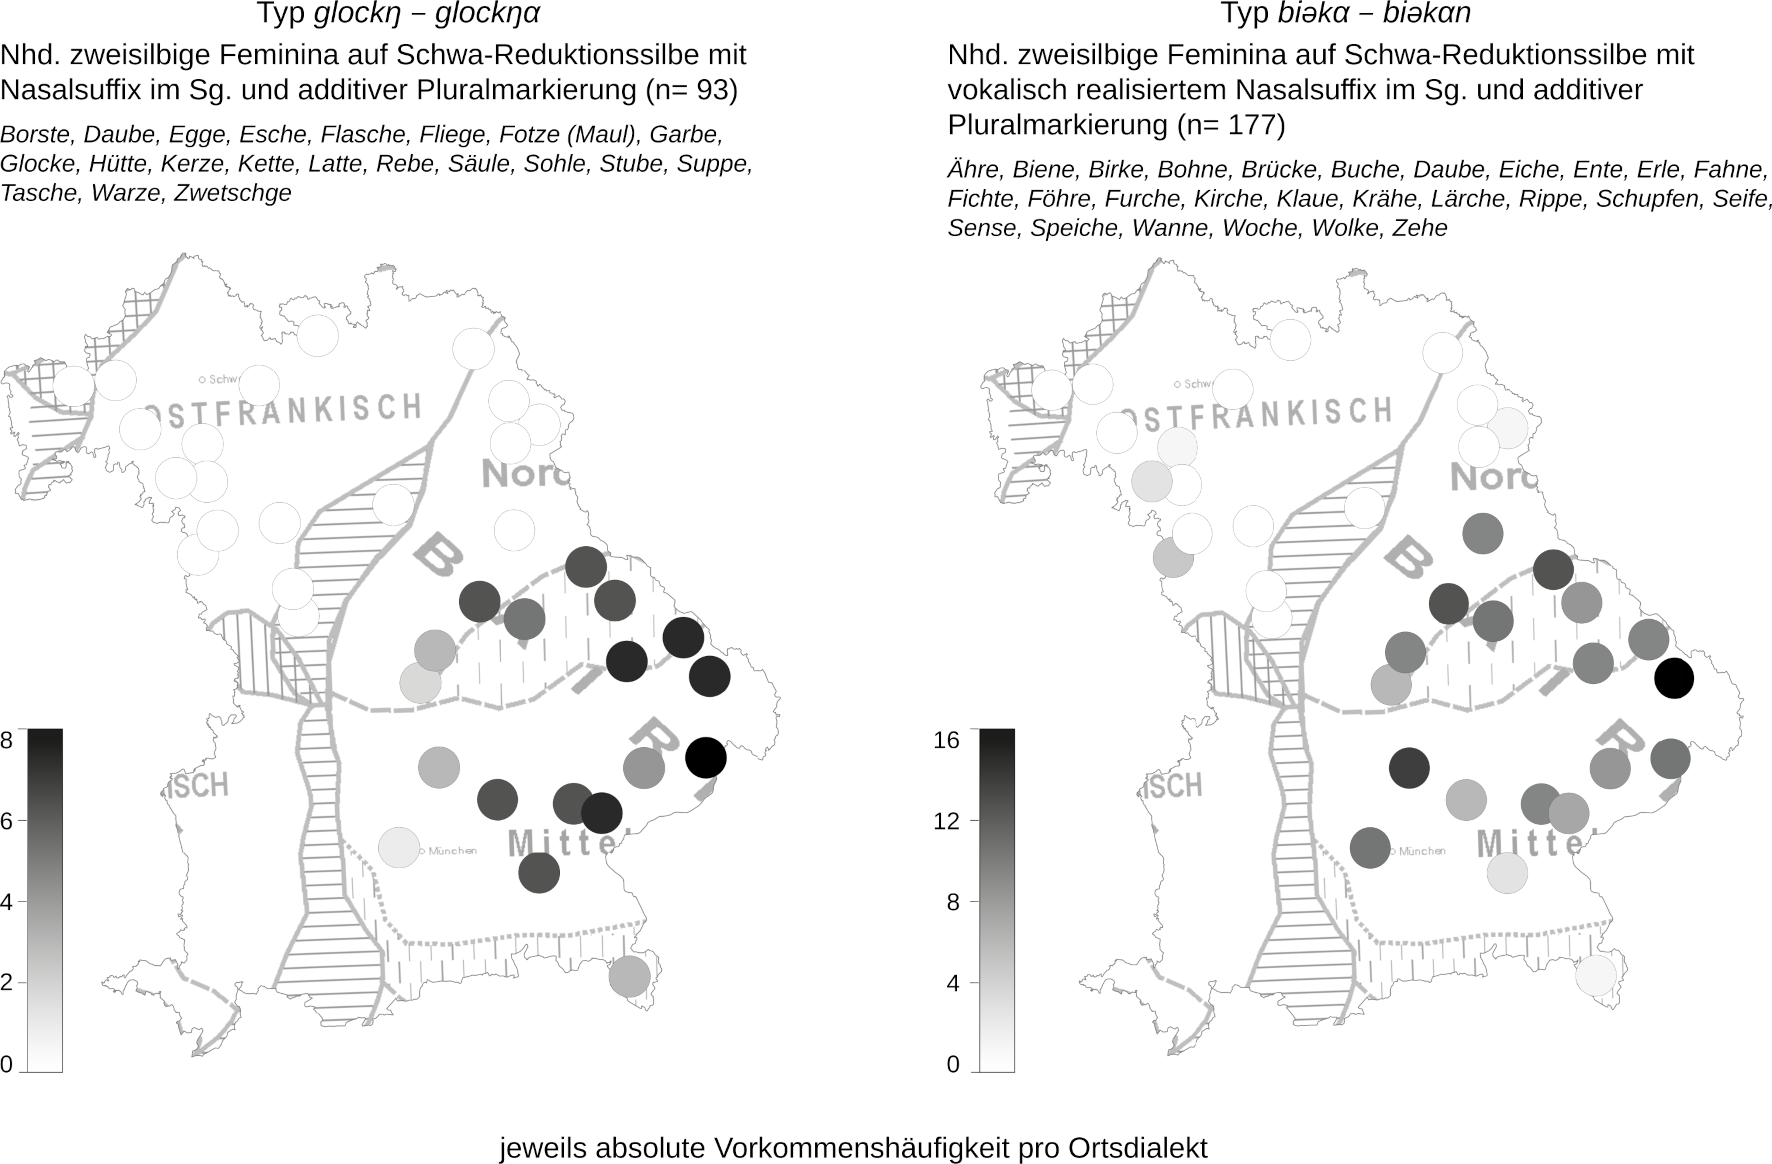
\includegraphics[width=\textwidth]{figures/Karte4.png}
\caption{Chloroplethkarten mit absoluter Vorkommenshäufigkeit additiver Pluralmarkierung bei nhd. zweisilbigen Feminina mit Schwa-Reduktionssilbe ($n=270$)}
\label{map:4}
\end{map}

\citet[131--132]{Mauser2000} zeigt in seiner Apparent-time-Studie für den bair. Dialekt des Salzburger Lungaus, dass die „innovativeren“ numerusdistinkten Formen mit Tiefschwa-Suffix in der älteren Sprechergeneration zu finden sind (z.\,B. \textit{ˈfaɪχtn̩} -- \textit{ˈfaɪχtnɐ} ‚Fichte‘, \textit{ˈloɪb̥m̩} -- \textit{ˈloɪb̥mɐ} ‚Loipe‘), während die jüngere Generation die „konservativeren“ synkretischen Formen verwendet. \citet[132]{Mauser2000} erklärt diesen Befund mit der stärkeren Normorientierung der jüngeren Sprechergeneration, die den „potentiellen Wandel“ blockiere (siehe auch \citealt[216]{Mauser1998a}). \citet[187--188]{Wildfeuer2001} kann in seiner Apparent-time-Studie eines mittelbair. Dialekts indes keine Tendenz zum Aus- oder Abbau der additiven Numerusmarkierung \textit{n}{}-erweiterter Feminina finden.\footnote{Bemerkenswert ist aber, dass auch \citet[218]{Wildfeuer2001} der jüngeren Sprechergeneration trotz einiger Um- und Abbautendenzen bei einzelnen Phänomenen „deutlich konservative Züge“ attestiert.}\largerpage[2]

\begin{sloppypar}
Der zweisilbigen Singularform der \textit{n}{}-erweiterten Feminina gleicht synchron die Struktur der zweisilbigen Maskulina mit Reduktionssilbe -\textit{en} (Typ \textit{Haufen}). Auch hier wird die Reduktionssilbe im gesamten UG in Abhängigkeit vom Stammauslaut als Nasal oder vokalisch realisiert, doch nur im südlichen Nordbair. und im Mittelbair. finden sich bei vokalisch realisierter Reduktionssilbe -\textit{α} additive Pluralformen mit Nasalsuffix: \teuthoo{ho.<v5A}{hôͅv̩α} -- \teuthoo{ho.<vAn}{hôͅvαn} ‚Hafen‘ (mittelbair. Grafenau), \teuthoo{ha4<o4v\%A}{hậọv͈α} -- \teuthoo{ha4<o4<v\%An}{hậộv͈αn} ‚Haufen‘ (mittelbair. Rei\-schach), \teuthoo{k,\_a.rpfA}{k͓ʰaͅrpfα} -- \teuthoo{k\_arpfAn}{kʰarpfαn} ‚Karpfen‘ (nordbair. Kallmünz), \teuthoo{k\_uAxA5}{kʰuαxα̩} -- \teuthoo{k\_uAxAn}{kʰuαxαn} ‚Kuchen‘ (nordbair.-mittelbair. Blaibach, vgl. \citealt[128 und 160]{Rowley1997}). \sectref{sec:8.3.3.1} wird zeigen, dass für die \textit{n}{}-Suffigierung bei femininen und maskulinen CVCV-Strukturen auf -\textit{α} von einem dialektraumspezifischen, produktiven Pluralbildungsmuster ausgegangen werden kann (siehe auch \sectref{sec:8.2.1} zur Deklination der historisch schwachen Maskulina in den rezenten Dialekten).
\end{sloppypar}

Daneben stellt auch die Abfolge aus Nasal im Stammauslaut und \textit{α}{}-Suffix in Pluralformen des Typs \teuthoo{s\#tu.mA}{štuͅmα} ein produktives Pluralbildungsmuster im Mittelbair. dar (inklusive der Übergangsgebiete zum Nord- und Südbair., siehe \citealt[166]{Mauser1998a}, \citealt[425]{Rowley1990b}, \citealt[128 und 160]{Rowley1997}, \citealt[58]{SMF7}, vgl. \citealt[§46h12]{Kranzmayer1956}). Diese Pluralformen mit Nasal+\textit{α} finden sich dabei auch für Feminina, deren Singularform kein Nasalsuffix aufweist, z.\,B. \teuthoo{nôo(+u(+d5}{n{\aufstrih}õ\klammerobenpost{}ũ\klammerobenpost{}d̩} -- \teuthoo{nôo(+u(+nA}{n{\aufstrih}õ\klammerobenpost{}ũ\klammerobenpost{}nα} ‚Naht‘ (nordbair. Oberdolling) und \teuthoo{s5a4<i:}{s̩ậi{\doubleogonek}} -- \teuthoo{s5a4<i:nA}{s̩ậi{\doubleogonek}nα} ‚Säule‘ (mittelbair.-südbair. Ramsau, siehe Abschnitte~\ref{sec:7.1.2.3.2} und \ref{sec:8.3.3.1}).\footnote{\citet[117]{Zehetner1985} nennt etwa noch die Form \textit{Frauna} (neben \textit{Frauan}) ‚Frauen‘, bei \citet[166]{Mauser2000} findet sich \textit{d̥ʀɔˑxd̥} -- \textit{ˈd̥ʀɔˑxt̺nɐ} ‚Tracht‘.}

Neben diesen Belegen für eine produktive Plural-Outputstruktur bei den Feminina finden sich nur für das schwache Maskulinum \textit{Bube} Pluralformen dieses Typs im nordbair.-mittelbair. Übergangsgebiet, vgl. \teuthoo{bo:u}{bo{\doubleogonek}u} -- \teuthoo{bo:umA}{bo{\doubleogonek}umα} -- \teuthoo{midn@}{midn̥} \teuthoo{bo:umAn}{bo{\doubleogonek}umαn} in Blaibach (vgl. \citealt[§38]{Kollmer1985}). Laut \citet[138]{Rowley1997} ist das \textit{α}{}-Suffix hier eine Form fakultativer Pluralmarkierung, die in dieser Form im südlichen Nordbair. und Mittelbair. sonst nur bei \textit{n}{}-erweiterten Feminina zu finden ist (\sectref{sec:9.2}). Diachron ist die Doppelsuffigierung das Ergebnis eines Assimilationsprozesses von Stammauslaut und Nasalsuffix in der Pluralform \textit{buben > bum}, die hier als „neue Grundgröße“ \citep[192]{Zehetner1978} die Basis für die „potenzierte“ additive Markierung bildet. Da auch nicht-assimilierte Singularformen wie \textit{lodn} ‚Latten‘ den Plural additiv mit Tiefschwa-Suffix bilden (Pl. \textit{lodna}), sieht \citet[123]{Steininger1994} Zehetners Argument einer Reanalyse der Wortstruktur infolge der Assimilation kritisch, die Ursache für die Suffigierung bestehe vielmehr darin, „daß der Pl. vom Sg. eindeutig unterschieden wird.“

\subsubsection{Suffixalternation}\label{sec:7.1.1.4}\largerpage
Für historisch zweisilbige Feminina der \textit{n}{}- und \textit{ô}{}-Deklination, die in der rezenten Singularform Nasalsuffix aufweisen, finden sich im mittelbair. Teil des UGs Belege für formal distinkte Singular- und Pluralformen, die sich im Suffix unterscheiden: \teuthoo{brukn}{brukn} -- \teuthoo{brukAn}{brukαn} ‚Brücke‘ (mittelbair. Wolfersdorf), \teuthoo{A}{α} \teuthoo{woi.k-N}{woiͅk{}͐ŋ} -- \teuthoo{woi.kA4n}{woiͅkα̣n} \teuthoo{E.}{əͅ} \teuthoo{hi9.me}{hi\klammeruntenpost{}ͅme} ‚Wolke/Wolken am Himmel‘ (mittelbair. Inning am Holz). Als additives Pluralmarkierungsverfahren stellen diese Suffixalternationen einen Grenzfall dar: Zwar sind -\textit{n} und \textit{{}-αn} jeweils segmentierbar, jedoch erfolgt die Numerusdifferenzierung nicht in Form einer Verkettung von Stammmorphem und Flexiv, als vielmehr in Form eines Austauschs der Morpheme. Die Form des Pluralsuffixes -\textit{αn} sowie die Pluralform als Ganzes entsprechen dabei der spezifischen Outputstruktur der Feminina im Bair. (vgl. \sectref{sec:8.3.3.1}).

Insgesamt finden sich im Korpus nur zwölf Belege dieser Suffixalternation \mbox{-\textit{n}} > -\textit{αn}, davon drei im mittelbair. Wolfersdorf und zwei im mittelbair. Waldhof. Die Alternation scheint im Mittelbair. insgesamt nur vereinzelt zu finden sein ($n=8$, vgl. \citealt[Karte 85 ‚Esche‘]{SOB4}). \citet[§572--573]{Schmeller1821} nennt einzelne Beispiele von Nominativ-Singular- und Pluralformen mit dem Suffix {}-\textit{ən} \mbox{(-\textit{αn})}, \citet[142]{Rowley1997} führt nur Belege für eine Alternation des Suffixes zwischen Nom. und Dat.Pl. in einem Gebiet im nördlichen Nordbair. und im Ofr. in der südlichen Fränkischen Schweiz an: Nom.Pl. \teuthoo{ga4rtn}{ɡạrtn} -- Dat.Pl. \teuthoo{ga4rtan}{ɡạrtan} ‚Gärten‘ (nordbair. Tirschenreuth), Nom.Pl. \teuthoo{ogsn}{oɡsn} -- Dat.Pl. \teuthoo{ogsan}{oɡsan} ‚Ochsen‘ (ofr. Pretzfeld), Nom.Pl. \teuthoo{gho.tSn}{ɡhoͅtʃn} -- Dat.Pl. \teuthoo{gho.tSan}{ɡhoͅtʃan} ‚Katzen‘ (nordbair. Neualbenreuth, vgl. \sectref{sec:7.2.1}). Suffixalternationen bei \textit{n}{}-erweiterten Feminina finden sich unterdessen auch im südlichen Arbeitsgebiet des SBS (d.\,h. im Schwäb. und mittelbair.-schwäb. Übergangsgebiet) in Form einer „geringen Aufhellung, die aber den Sprechern deutlich bewusst ist“ \citep[64]{Freudenberg1959}, von -\textit{ə} zu -\textit{α}/\textit{a}: \teuthoo{A}{α} \teuthoo{nu.<iE@}{nûͅiə̥} \teuthoo{glo4kE}{ɡlọkə} -- \teuthoo{nu.<iE@}{nûͅiə̥} \teuthoo{glo4ka}{ɡlọka} ‚(eine) neue Glocke(n)‘ im schwäb. Bernbeuren (vgl. \mapref{map:33}, \citealt[8]{Rowley1994}, \citealt[261--262 sowie Karten 105--113]{SBS9.1}).

Ein weiterer Fall von Suffixalternation findet sich im Ofr., wo Diminutiva gebietsweise unterschiedliche Diminutivsuffixe in der Singular- und Pluralform aufweisen: -\textit{la}/-\textit{le} im Singular, -\textit{li}/-\textit{liX} im Plural, z.\,B.: \teuthoo{ma42dlA}{mạ̄dlα} -- \teuthoo{ma42dJi.}{mạ̄d{\lkreis}iͅ} ‚Mädchen‘ (ofr. Burgbernheim), \teuthoo{mu?glE}{müɡlə} -- \teuthoo{mu?gli.c}{müɡliX} ‚Mücke‘ (ofr. Gemünden am Main, vgl. \citealt[Karte 34]{Rowley1997}, \citealt[22--23 und Karte 45]{SMF7}, \citealt[Karte 54]{SUF3}, \citealt{WA}-Karte 381 „Apfelbäumchen“). Numerusdifferenzierung findet hier an der Schnittstelle von Flexionsmorphologie und Wortbildung statt, sodass sich die Frage stellt, in welchem Bereich der Morphologie die einzelnen Diminutiv-Flexionsformen in der Analyse stärker verortet werden.

Historisch werden die verschiedenen Suffixe der Singular- und Pluralformen auf verschiedene Derivationssuffixe zurückgeführt:

\begin{itemize}
\item Die Suffixformen -\textit{la}/-\textit{le} im Singular gehen auf das Diminutivsuffix mhd. -\textit{lîn} zurück, das im UG weitestgehend mit elidiertem auslautendem Nasal erscheint.
\item Die Pluralsuffixe -\textit{li}/-\textit{liX} könnten auf ein kollektivierendes Derivationssuffix zurückgehen (\citealt[§596--606]{Schmeller1821}, \citealt[112]{Wrede1908}, vgl. \citealt[24--25]{Rowley1994}, \citealt[194--195]{SMF7}).
\item Im Nordbair. und im ofr.-nordbair. Übergangsgebiet erscheint im Plural das Suffix -\textit{la}, das ebenfalls auf ein Kollektivsuffix (-\textit{lach}) zurückgeht (\citealt[22--24]{Rowley1994}, vgl. \citealt[1253]{Seebold1983}).
\end{itemize}

Wenngleich die Diminutiva historisch auf unterschiedliche Derivationssuffixe zurückgehen, wird synchron in einem Streifen im östlichen Ofr. formal nicht zwischen Singular und Plural unterschieden: Typ \teuthoo{A}{α} \teuthoo{va94sla94}{va\klammeruntenpost{}̣sla\klammeruntenpost{}̣} -- \teuthoo{va94sla94}{va\klammeruntenpost{}̣sla\klammeruntenpost{}̣} ‚Fass‘ (ofr. Ahorn, vgl. \citealt[Karte 33]{Rowley1997}, \citealt[Karten 63.1/2]{Steger1968}). Im Nordbair. (inklusive Übergangsgebiete) ist dagegen der Typ \teuthoo{bri.kl@}{briͅkl̥} -- \teuthoo{bri.klA}{briͅklα} ‚Brücke‘ (nordbair. Groschlattengrün) verbreitet mit Diminutivsuffix -\textit{(ə)l} im Singular und -\textit{la} im Plural. Daneben finden sich synkretische Formen und Formen mit Nasalsuffix, und zwar teilweise nebeneinander, vgl. die Formen \teuthoo{a42dAl@}{ạ̄dαl̥} -- \teuthoo{a42dAlA}{ạ̄dαlα}, \teuthoo{a42dAln}{ạ̄dαln}, \teuthoo{a42dAl}{ạ̄dαl} ‚Ader‘ im nordbair.-mittelbair. Zwiesel. \citet[136]{Rowley1997} zufolge stellen die Plurale auf -\textit{a} die älteren, jene auf -\textit{n} die jüngeren Formen dar.

\begin{sloppypar}
In der Klassifikation des SMF werden Diminutivbildungen des Typs \teuthoo{bri.kl@}{briͅkl̥} -- \teuthoo{bri.klA}{briͅklα} zur Pluralmarkierung durch unterschiedliche Diminutivsuffixe gezählt und damit stärker der Wortbildung zugerechnet (\citealt[204]{SMF7}). Alternativ zu dieser Klassifikation, die die diachrone Entwicklung des Diminutivsuffixes bewahrt, analysiere ich diesen Typus im Sinne einer synchronen Klassifikation als additive Pluralmarkierung mit Nasal- bzw. Tiefschwa-Suffix. Auch wenn die rezenten Diminutivformen diachron auf eine Alternation der Suffixe im Singular und Plural zurückgehen, scheint diese Analyse hier vorteilhafter, denn sie  ermöglicht es, die Formen \teuthoo{a42dAlA}{ạ̄dαlα} und \teuthoo{a42dAln}{ạ̄dαln} gleichermaßen als additive Plurale zu klassifizieren: Sowohl \textit{α}{}- als auch Nasalsuffix gehören zum dialektalen Pluralmarkerinventar in diesem Teil des UGs und stellen damit produktive Pluralbildungsverfahren dar (vgl. \citealt[1199]{Dingeldein1983}).
\end{sloppypar}

\subsection{Stammaffizierende Markierung}
\label{sec:7.1.2}
Zur stammaffizierenden Markierung zählen jene Pluralmarkierungsverfahren, die nicht in einer Verkettung von Morphemen bestehen, sondern die die lautliche Form des Stammes verändern. In den untersuchten Dialekten gehören hierzu Markierungsstrategien, die den Vokalismus oder Konsonantismus des Stammes affizieren, subtraktive Verfahren und kombinierte Markierungen (d.\,h. die kumulative Kombination verschiedener additiver und/oder stammaffizierender Verfahren). Morphologie vollzieht sich hier an der Schnittstelle zum phonologischen System: Stammaffizierende Markierung ist das Ergebnis phonologisch bedingter Alternationen im Flexionsparadigma, die teilweise historische phonologische Prozesse konservieren, teilweise aber auch in den phonologischen Systemen der rezenten Dialekte wirksam sind. Die diachrone Perspektive zeigt hier auf, inwiefern das phonologische System der einzelnen Dialekte Voraussetzung für spezifische morphophonologische Verfahren ist. So sind in Dialekten, die zwar die Einsilberdehnung vollzogen, aber keine Lenis-Fortis-Oppositionen im phonologischen System bewahrt haben, innerparadigmatische Alternationen der Vokalquantität morphologisiert. Dialekte mit Lenis-Fortis-Kontrasten hingegen haben diese neben oder in Kombination mit Quantitätskontrasten funktionalisiert.

Ziel der folgenden Kapitel ist es, das konkrete Inventar stammaffizierender Pluralmarkierungsstrategien auszuweisen und gleichzeitig zu zeigen, inwiefern sie durch dialektspezifische Lautentwicklungen und phonologische Prozesse bedingt sind. Im Einzelfall wird zu entscheiden sein, ob rezente innerparadigmatische Alternationen primär phonologisch bedingt sind, ob sie eine lexikalisierte morphophonologische Alternation darstellen oder ob sie als morphologische Markierungsstrategien funktionalisiert und produktiv sind.

\subsubsection{Kontraste der Vokalqualität}
\label{sec:7.1.2.1}
Kontraste der Vokalqualität stellen im UG ein ausgesprochen frequentes Pluralmarkierungsverfahren dar. Neben dem Umlaut als dem „allgemeinsten Bildungsmittel des Plurals“ \citep[1086]{Lüssy1983} in den hd. Dialekten finden sich der umlautähnliche Diphthongwechsel bei Lexemen mit dem Stammvokal mhd. \textit{ei} (\sectref{sec:7.1.2.1.2}) sowie innerparadigmatische Wechsel der Zungenhöhe (\sectref{sec:7.1.2.1.3}). Auf diachrone phonologische Entwicklungen des Vokalsystems wird nur dann im Detail zurückgegriffen, wenn es für die Fragestellung relevant ist. Für eine detaillierte Aufführung der historischen phonologischen Entwicklungen im Vokalismus in den einzelnen Tiefenbohrungspunkten sei an dieser Stelle auf die relevanten BSA-Bände verwiesen.

\subsubsubsection{Umlaut}
\label{sec:7.1.2.1.1}
Der Umlaut stellt als „Paradebeispiel“ (\citet[57]{Rowley1997} eines innerparadigmatischen Vokalwechsels die frequenteste Form stammaffizierender Morphologie im UG dar. Historisch bezeichnet der Umlaut die assimilatorische Palatalisierung (auch Frontierung, vgl. etwa \citealt{Wiese1987}) eines hinteren Vokals unter Einfluss eines /i/ oder /j/ in der Folgesilbe (vgl. \citealt[194--199]{Schirmunski1962}, \sectref{sec:3.1.1}). Auch synchron entspricht der Umlaut einem Wechsel von velarem zu palatalem Vokal, das spezifische Wechselmuster des Umlauts besteht nach \citet[57]{Rowley1997} dabei idealiter in der „vollen“ Korrelation der Zungenhöhe. Das Prinzip der Zungenhöhenkorrelation stelle dabei auch diachron ein stabiles Merkmal dar, da die phonologischen Entwicklungen der Vokalsysteme der nordostbayrischen Dialekte die vorderen und hinteren Vokalreihen gleichermaßen betreffe oder die Korrelation im Falle von mhd. \textit{a}, \textit{â} durch Ausgleich hergestellt werden könne (\citealt[57--66]{Rowley1997}, vgl. \citealt[47]{Steger1968}). Zu einer Aufhebung der „vollen“ Zungenhöhenkorrelation führt dagegen die Dehnung des Basisvokals infolge der Einsilberdehnung, da der Quantitätskontrast als weiteres phonologisches Merkmal hinzukommt \citep[67]{Rowley1997}.

\citet[117]{Rowley1997} bestätigt für die Dialekte Nordostbayerns den Befund \citegen{Moulton1971} für das Schweizerdeutsche: Das morphophonologische Prinzip des Umlauts besteht in der Alternation zwischen velarem und palatalem Vokal und damit in der Modulation der Merkmalsopposition [±palatal]. Analoge Umlautformen sind stets korrelierende Umlaute, d.\,h. die Merkmalsopposition [±palatal] ist morphologisiert \citep[117]{Rowley1997}. Von korrelierenden Umlauten sind nach \citet[118]{Rowley1997} teilkorrelierende Umlaute zu unterscheiden, die neben der Modulation des Merkmals [±palatal] Variation in einem weiteren phonologischen Merkmal aufweisen (nämlich Rundung, Öffnung oder Vokalquantität). Nicht-korrelierende Umlaute weichen daneben in gleich mehreren phonologischen Merkmalen ab.

Die folgenden Detailanalysen mit Bezug auf das mhd. Vokalsystem werden zeigen, dass die Umlautrelationen dialektspezifisch sind und im interdialektalen Vergleich variieren. Zu unterscheiden sind Systeme, in denen historisch eine Reduktion der Vokalalternanzen stattgefunden hat, und Systeme, in denen diachron eine lautgesetzlich bedingte Ausdifferenzierung der Vokalalternanzen erfolgt ist. Die Oppositionen in den rezenten Vokalsystemen und damit auch die dialektalen Umlautmöglichkeiten sind jeweils das Ergebnis historischer phonologischer Prozesse, die den Stammvokalismus affizieren (in diesem Zusammenhang insbesondere Rundung/Entrundung, Monophthongierung/Diphthongierung), von Aufhebung von Oppositionen (d.\,h. Zusammenfall von Lauten) und von Phonemspaltungen (vgl. \citealt[1084]{Lüssy1983}, \citealt[117]{Rowley1997}, \citealt[200--202]{Schirmunski1962}, \citealt[1046]{Wiesinger1983d}).

\subsubsubsubsection{Rezente Umlautentsprechungen vor dem Hintergrund des mhd. Protosystems}
In \figref{fig:4} werden die rezenten Umlautentsprechungen für fünf exemplarische Ortsdialekte im ofr. Rundungsgebiet (Erlabrunn), im ofr. Entrundungsgebiet (Wilhermsdorf), im Nordbair. (Windischeschenbach) und im Mittelbair. (Kirchensur) getrennt für die mhd. Vokalreihen dargestellt. Die Anordnung der Umlautmöglichkeiten entspricht der Anordnung im Vokaltrapez, d.\,h. die velaren Basisvokale sind in den einzelnen Grafiken rechts zu finden, die palatalen Umlautvokale links. Basis- und Umlautvokale wurden nach Quantität differenziert. Anders als \citet[1049]{Wiesinger1983d} setze ich keine quantitätslosen Vokalsysteme für das Nord- und Mittelbair. an, da Quantitäts- und Lenis-Fortis-Kontraste unabhängig voneinander realisiert werden können (vgl. \sectref{sec:7.1.2.3.1}).




\begin{sidewaysfigure}
\small
\begin{tabularx}{\textwidth}{@{}Qp{2.5cm}p{2cm}>{\centering}p{3.5cm}p{2cm}@{}}
 & ofr.\newline Wilhermsdorf & ofr.\newline Erlabrunn & nordbair.\newline Windischeschenbach   & mittelbair.\newline  Kirchensur \\
 \hline
%  \parbox[b]{4cm}{
 \textbf{mhd. i--ü--u, î--iu--û}\newline\footnotesize
  Fuchs, Hund, Nuss, Sohn, Strumpf, Stube, Turm, Wurm, Wurst, Wurzel; \newline
  Bauch, Faust, Haufen, Haus, Haut, Maul, Maus, Sau, Strauß, Zaun
%   }
    &
    \begin{tikzpicture}[baseline=(i.base),every node/.style={inner sep=0,outer sep=0}]
      \node(i){i\strut};
      \node(e)[below=0mm of i]{e \strut};
      \node(ea)[below=0mm of e]{eα \strut};
      \node(ae)[below=0mm of ea]{ae \strut};


      \node(u)[right=10mm of i]{u\strut};
      \node(o)[below=0mm of u]{o\strut};
      \node(oa)[below=0mm of o]{oα\strut};
      \node(ao)[below=0mm of oa]{ao\strut};

      \draw(i.east)--(u.west);
      \draw(e.east)--(o.west);
      \draw(ea.east)--(oa.west);
      \draw(ae.east)--(ao.west);
    \end{tikzpicture}
    &
    \begin{tikzpicture}[baseline=(ü.base),every node/.style={inner sep=0,outer sep=0}]
      \node(ü){ü\strut};
      \node(none1)[below=0mm of ü]{~\strut};
      \node(ö)[below=0mm of none1]{ö \strut};
      \node(öö)[below=0mm of ö]{\=ö \strut};
      \node(aü)[below=0mm of öö]{aü \strut};
      \node(ai)[below=0mm of aü]{ai \strut};


      \node(u)[right=10mm of i]{u\strut};
      \node(uu)[below=0mm of u]{\=u\strut};
      \node(o)[below=0mm of uu]{o\strut};
      \node(oo)[below=0mm of o]{\=o\strut};
      \node(ao)[below=2mm of oo]{ao\strut};

      \draw(ü.east)--(u.west);
      \draw[dotted,thick](ü.east)--(uu.west);
      \draw[dotted,thick](ö.east)--(u.west);
      \draw(ö.east)--(o.west);
      \draw(öö.east)--(oo.west);
      \draw[dotted,thick](ö.east)--(ao.west);
      \draw[dotted,thick](ö.east)--(oo.west);
      \draw(aü.east)--(ao.west);
      \draw(ai.east)--(ao.west);
    \end{tikzpicture}
    &
    \begin{tikzpicture}[baseline=(i.base),every node/.style={inner sep=0,outer sep=0}]
      \node(i){i\strut};
      \node(iie)[below=0mm of i]{{\=\i}ǝ \strut};
      \node(none1)[below=0mm of iie]{~\strut};
      \node(aai)[below=0mm of none1]{\=ai \strut};
      \node(ai)[below=0mm of aai]{ai \strut};


      \node(u)[right=10mm of i]{u\strut};
      \node(uue)[below=0mm of u]{{\=u}ə\strut};
      \node(aa)[below=0mm of uue]{\={ạ}\strut};
      \node(aao)[below=0mm of aa]{\=ao\strut};

      \draw(i.east)--(u.west);
      \draw(iie.east)--(uue.west);
      \draw(aai.east)--(aao.west);
      \draw[dotted,thick](ai.east)--(aa.west);
      \draw[dotted,thick](ai.east)--(aao.west);
    \end{tikzpicture}
    &
      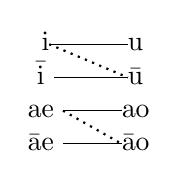
\begin{tikzpicture}[baseline=(i.base),every node/.style={inner sep=0,outer sep=0}]
      \node(i){i\strut};
      \node(ii)[below=0mm of i]{\=i \strut};
      \node(ae)[below=0mm of ii]{ae \strut};
      \node(aae)[below=0mm of ae]{\=ae \strut};


      \node(u)[right=10mm of i]{u\strut};
      \node(uu)[below=0mm of u]{\=u\strut};
      \node(ao)[below=0mm of uu]{ao\strut};
      \node(aao)[below=0mm of ao]{\=ao\strut};

      \draw(i.east)--(u.west);
      \draw(ii.east)--(uu.west);
      \draw(ae.east)--(ao.west);
      \draw(aae.east)--(aao.west);
      \draw[dotted,thick](i.east)--(uu.west);
      \draw[dotted,thick](ae.east)--(aao.west);
    \end{tikzpicture}\\
    \hline
\textbf{mhd. e--ö--o, ê--œ--ô}\newline\footnotesize
Bock, Boden, Borste, Dof, Dorn ,Forsch, Bbel, Horn, Joch, Knophf, Knoten, Kopf, Korb, Korn, Kfroph, Loch, Ofen, Rock, Schloss, Stock, Tochter, Tropf, Trog, Vogel, Zopf;\newline
Floh, Kloß, Lohn, Ohr &
    \begin{tikzpicture}[baseline=(i.base),every node/.style={inner sep=0,outer sep=0}]
      \node(e){e\strut};
      \node(ee)[below=0mm of e]{\=e \strut};
      \node(none1)[below=0mm of ee]{~ \strut};

      \node(o)[right=10mm of i]{o\strut};
      \node(oo)[below=0mm of o]{\=o\strut};
      \node(aa)[below=0mm of oo]{\=a\strut};

      \draw(e.east)--(o.west);
      \draw(ee.east)--(oo.west);
      \draw(ee.east)--(aa.west);
      \draw[dotted,thick](e.east)--(oo.west);
    \end{tikzpicture}
    &
    \begin{tikzpicture}[baseline=(i.base),every node/.style={inner sep=0,outer sep=0}]
      \node(ö){ö\strut};
      \node(none1)[below=0mm of ö]{~ \strut};
      \node(ööi)[below=0mm of none1]{\=öï\strut};
      \node(ööa)[below=0mm of ööi]{\=öα\strut};

      \node(o)[right=10mm of ö]{o\strut};
      \node(oo)[below=0mm of o]{\=o\strut};
      \node(oou)[below=0mm of oo]{\=ou\strut};
      \node(ooa)[below=0mm of oou]{\=oα\strut};

      \draw(ö.east)--(o.west);
      \draw(ööi.east)--(oou.west);
      \draw(ööa.east)--(ooa.west);
      \draw[dotted,thick](ö.east)--(oo.west);
      \draw[dotted,thick](ö.east)--(oou.west);
      \draw[dotted,thick](ö.east)--(ooa.west);
    \end{tikzpicture}
    &
    \begin{tikzpicture}[baseline=(ü.base),every node/.style={inner sep=0,outer sep=0}]
      \node(iie){\=iə\strut};
      \node(e)[below=0mm of iie]{e};
      \node(eea)[below=0mm of e]{{\=e}α  \strut};
      \node(eei)[below=0mm of eea]{\=ei \strut};
      \node(a)[below=0mm of eei]{ạ \strut};

      \node(uue)[right=10mm of i]{{\=u}ə\strut};
      \node(ooo)[below=2mm of uue]{\aufstrich\=oo\strut};
      \node(ooa)[below=2mm of ooo]{\=oα\strut};

      \draw(iie.east)--(uue.west);
      \draw(eea.east)--(ooa.west);
      \draw[dotted,thick](e.east)--(uue.west);
      \draw[dotted,thick](eei.east)--(ooo.west);
      \draw[dotted,thick](eei.east)--(ooa.west);
      \draw[dotted,thick](a.east)--(ooa.west);
    \end{tikzpicture}
    &
    \begin{tikzpicture}[baseline=(ü.base),every node/.style={inner sep=0,outer sep=0}]
      \node(i){i\strut};
      \node(none1)[below=0mm of i]{~\strut};
      \node(e)[below=0mm of none1]{e \strut};
      \node(ee)[below=0mm of e]{\=e \strut};

      \node(none2)[right=10mm of i]{~\strut};
      \node(uu)[below=0mm of none2]{\=u\strut};
      \node(o)[below=0mm of uu]{o\strut};
      \node(oo)[below=0mm of o]{\=o\strut};
      \node(oou)[below=0mm of oo]{\aufstrich\=ou\strut};

      \draw(e.east)--(o.west);
      \draw(ee.east)--(oo.west);
      \draw[dotted,thick](i.east)--(uu.west);
      \draw[dotted,thick](e.east)--(oo.west);
      \draw[dotted,thick](ee.east)--(oou.west);
    \end{tikzpicture}\\
    \textbf{mhd. a, â, ë, ä æ}\newline\footnotesize
    Acker, Apfel, Ast, Bach, Band, Bank, Blatt, Dach, Darm, Faden, Fass, Gabel, Gang, Gans, Garten, Glas, Grab, Grabene, Hafen, Hammer, Hand, Kalb, Kamm, Karren, Magd, Magen, Mann, Markt, Nacht, Nagel, Name, Rad, Sack, Schlag, Schnabel, Schwanz, Stadt, Stall, Start, Tag, Wade, Wagen, Wald, Wasen, Zahn;\newline
    Draht, Naht, Pfahl, Schaf, Straße
    &
    \begin{tikzpicture}[baseline=(i.base),every node/.style={inner sep=0,outer sep=0}]
      \node(e){e\strut};
      \node(ee)[below=0mm of e]{\=e \strut};

      \node(o)[right=10mm of e]{o\strut};
      \node(oo)[below=0mm of o]{\=o\strut};
      \node(a)[below=0mm of oo]{a\strut};
      \node(aa)[below=0mm of a]{\=a\strut};

      \draw(e.east)--(o.west);
      \draw(e.east)--(a.west);
      \draw(ee.east)--(oo.west);
      \draw(ee.east)--(aa.west);
      \draw[dotted,thick](e.east)--(oo.west);
    \end{tikzpicture}
    &
    \begin{tikzpicture}[baseline=(i.base),every node/.style={inner sep=0,outer sep=0}]
      \node(ö){ö\strut};
      \node(e)[below=0mm of ö]{e \strut};
      \node(ee)[below=0mm of e]{\=e \strut};
      \node(eei)[below=0mm of ee]{\=ei \strut};
      \node(ööa)[below=0mm of eei]{\=öα \strut};
      \node(eea)[below=0mm of ööa]{\=eα \strut};
      \node(a1)[below=0mm of eea]{\d{a} \strut};
      \node(aa1)[below=0mm of a1]{\=a \strut};


      \node(oo)[right=10mm of ee]{\=o\strut};
      \node(ooa)[right=10mm of ööa]{\=oα\strut};
      \node(a2)[right=10mm of a1]{a\strut};
      \node(aa2)[right=10mm of aa1]{\=a\strut};

      \draw(e.east)--(aa2.west);
      \draw(ee.east)--(oo.west);
      \draw(ee.east)--(aa2.west);
      \draw(ööa.east)--(ooa.west);
      \draw(eea.east)--(ooa.west);
      \draw(a1.east)--(a2.west);
      \draw(aa1.east)--(oo.west);
      \draw[dotted,thick](ö.east)--(oo.west);
      \draw[dotted,thick](ö.east)--(ooa.west);
      \draw[dotted,thick](ö.east)--(a2.west);
      \draw[dotted,thick](e.east)--(oo.west);
      \draw[dotted,thick](e.east)--(aa2.west);
      \draw[dotted,thick](eei.east)--(aa2.west);
      \draw[dotted,thick](a1.east)--(oo.west);
      \draw[dotted,thick](aa1.east)--(ooa.west);
    \end{tikzpicture}
    &
    \begin{tikzpicture}[baseline=(i.base),every node/.style={inner sep=0,outer sep=0}]
      \node(iie){\=iə\strut};
      \node(e)[below=0mm of iie]{e \strut};
      \node(ee)[below=0mm of e]{\=e \strut};
      \node(eei)[below=0mm of ee]{\=ei \strut};
      \node(a)[below=0mm of eei]{\d{a} \strut};
      \node(aa)[below=0mm of a]{\d{\=a} \strut};
%

      \node(none1)[right=10mm of iie]{~\strut};
      \node(o)[below=2mm of none1]{\=o\strut};
      \node(ooo)[below=0mm of o]{\aufstrich\=oo\strut};
      \node(ooa)[below=0mm of ooo]{\=oα\strut};
      \node(oa)[below=0mm of ooa]{\burgeroa\strut};

      \draw(ee.east)--(o.west);
      \draw(a.east)--(oa.west);
      \draw(aa.east)--(o.west);
      \draw[dotted,thick](iie.east)--(o.west);
      \draw[dotted,thick](e.east)--(o.west);
      \draw[dotted,thick](eei.east)--(ooo.west);
      \draw[dotted,thick](a.east)--(ooa.west);
    \end{tikzpicture}
    &
    \begin{tikzpicture}[baseline=(i.base),every node/.style={inner sep=0,outer sep=0}]
      \node(e){e\strut};
      \node(ee)[below=0mm of e]{\=e \strut};
      \node(a)[below=0mm of ee]{\d{a} \strut};
      \node(aa)[below=0mm of a]{\d{\=a} \strut};

      \node(o)[right=10mm of e]{o\strut};
      \node(oo)[below=0mm of o]{\=o\strut};
      \node(a2)[below=0mm of oo]{\k{a}\strut};

      \draw(e.east)--(o.west);
      \draw(e.east)--(a2.west);
      \draw(ee.east)--(oo.west);
      \draw(a.east)--(a2.west);
      \draw(aa.east)--(oo.west);
      \draw[dotted,thick](e.east)--(oo.west);;
    \end{tikzpicture}\\
    \textbf{mhd. ie--üe--uo}\newline\footnotesize
    Bruder, Fuß, Huhn, Hut, Krug, Kuh, Mutter, Pflug, Stuhl
    &
    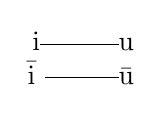
\begin{tikzpicture}[baseline=(i.base),every node/.style={inner sep=0,outer sep=0}]
      \node(i){i\strut};
      \node(ii)[below=0mm of i]{\=i \strut};


      \node(u)[right=10mm of i]{u\strut};
      \node(uu)[below=0mm of u]{\=u\strut};

      \draw(i.east)--(u.west);
      \draw(ii.east)--(uu.west);
    \end{tikzpicture}
    &
    \begin{tikzpicture}[baseline=(i.base),every node/.style={inner sep=0,outer sep=0}]
      \node(üüe){\=üə\strut};
      \node(ö)[below=0mm of üüe]{ö \strut};
      \node(ööa)[below=0mm of ö]{\=öα \strut};


      \node(uue)[right=10mm of üüe]{\=uə\strut};
      \node(none1)[below=0mm of uue]{~\strut};
      \node(ooa)[below=0mm of none1]{oα\strut};

      \draw(üüe.east)--(uue.west);
      \draw(ööa.east)--(ooa.west);
      \draw[dotted,thick](ö.east)--(uue.west);
      \draw[dotted,thick](ööa.east)--(uue.west);
    \end{tikzpicture}
    &
    \begin{tikzpicture}[baseline=(i.base),every node/.style={inner sep=0,outer sep=0}]
      \node(none1){~\strut};
      \node(eei)[below=0mm of none1]{\=ei \strut};
      \node(ei)[below=0mm of eei]{ei \strut};

      \node(ööu)[right=10mm of üüe]{\aufstrich\=öu\strut};
      \node(oou)[below=0mm of ööu]{\aufstrich\=ou\strut};

      \draw(eei.east)--(oou.west);
      \draw[dotted,thick](eei.east)--(ööu.west);
      \draw[dotted,thick](ei.east)--(ööu.west);
    \end{tikzpicture}
    &
    \begin{tikzpicture}[baseline=(i.base),every node/.style={inner sep=0,outer sep=0}]
      \node(none1){~\strut};
      \node(iia)[below=0mm of none1]{\=iα \strut};

      \node(ua)[right=10mm of none1]{uα\strut};
      \node(uua)[below=0mm of ua]{\=uα\strut};

      \draw(iia.east)--(uua.west);
      \draw[dotted,thick](iia.east)--(ua.west);
    \end{tikzpicture}
    \\
    \textbf{mhd. ei--öu--ou}\newline\footnotesize
    Baum, Reifen
    &
    \begin{tikzpicture}[baseline=(i.base),every node/.style={inner sep=0,outer sep=0}]
      \node(e){e\strut};
      \node(a)[right=10mm of e]{a\strut};
      \draw(e.east)--(a.west);
    \end{tikzpicture}
    &
    \begin{tikzpicture}[baseline=(i.base),every node/.style={inner sep=0,outer sep=0}]
      \node(ö){ö\strut};
      \node(aa)[right=10mm of ö]{\=a\strut};
      \draw(ö.east)--(aa.west);
    \end{tikzpicture}
    &
    \begin{tikzpicture}[baseline=(i.base),every node/.style={inner sep=0,outer sep=0}]
      \node(ai){âi\strut};
      \node(a)[right=10mm of ai]{\d{a}\strut};
      \draw[dotted,thick](ai.east)--(a.west);
    \end{tikzpicture}
    &
    \begin{tikzpicture}[baseline=(i.base),every node/.style={inner sep=0,outer sep=0}]
      \node(ea){eα};
      \node(oa)[right=10mm of ea]{oα\strut};
      \draw(ea.east)--(oa.west);
    \end{tikzpicture}\\



\end{tabularx}
  \caption{Rezente Umlautentsprechungen in exemplarischen Ortsdialekten mit mhd. Bezugssystem ($n=342$)\label{fig:4}}
\end{sidewaysfigure}

Die Umlautvokale unterscheiden sich in jenen Dialekten, in denen die Rundung der mhd. Bezugsvokale bewahrt wurde, von jenen, in denen Entrundung eingetreten ist, z.\,B. mhd. \textit{o}/\textit{ö} in \teuthoo{khôo.<ubv}{kh{\aufstrih}ôͅubv} -- \teuthoo{kho?bv}{khöbv} ‚Kopf‘ im ofr. Erlabrunn vs. \teuthoo{k\_o94bv5}{kʰo\klammeruntenpost{}̣bv̩} -- \teuthoo{khÔe:bv5}{kh{\doppelaufstrih}e{\doubleogonek}bv̩} im ofr. Wilhermsdorf. Entrundung der palatal-gerundeten Vokale findet sich im größten Teil des UGs, bewahrt ist Rundung im Unterofr. bis hinein in den Henneberger Raum und das Osthessische.\footnote{Vgl. \citet[67--68 und Karte 13]{Rowley1997}, \citet[204--208]{Schirmunski1962}, \citet[41--43 und Karten 22/31]{Steger1968}, \citet[1103]{Wiesinger1983e} sowie \citealt{WA}-Karte 465 „Häuser“.} Im Entrundungsgebiet werden die mhd. Umlautvokale \textit{ö}, \textit{ü}, \textit{iu} usw. ungerundet realisiert und sind mit mhd. \textit{e}, \textit{i}, \textit{î} usw. zusammengefallen, vgl. mhd. \textit{o}/\textit{ö} in \teuthoo{v5ro42s\#}{v̩rọ̄š} -- \teuthoo{v5re?S'}{v̩rëʃ̌} ‚Frosch‘ vs. mhd. \textit{a}/\textit{e} in \teuthoo{gða.ns}{ɡ̩aͅns} -- \teuthoo{gðens}{ɡ̩ens} ‚Gans‘ im mittelbair. Kirchensur (vgl. \citealt[§4a4]{Kranzmayer1956}, \citealt[1102]{Wiesinger1983e}).

In Rundungsdialekten finden sich gerundete Vorderzungenvokale als Basisvokale in nur wenigen Lexemen; wesentlich frequenter sind sie als Umlautprodukte in Flexionsformen, weshalb sie „deutliche Exponenten“ \citep[68]{Rowley1997} flexivischer Information darstellen. In diesen Dialekten kann Rundung in Kombination mit dem Umlaut als morphophonologischer Marker auch bei historisch palatal-ungerundeten Vokalen auftreten. Der palatal-gerundete Umlautvokal \textit{ö} (neben der diphthongischen Variante \teuthoo{o?"A}{ȫα}) findet sich in den Rundungsdialekten für alle historischen Vokalreihen, und zwar auch „an historisch unberechtigter Stelle“ \citep[68]{Rowley1997}. Dies gilt nach \citet[1103]{Wiesinger1983e} vor allem in der phonologischen Umgebung von Konsonanten mit Lippenrundung (\textit{b}/\textit{p}, \textit{w}, \textit{f}, \textit{š} und Affrikate \textit{bf}/\textit{pf}), beispielsweise bei \teuthoo{a.bv5l@}{aͅbv̩l̥} -- \teuthoo{o?bv5l@}{öbv̩l̥} -- Dim. \teuthoo{o?bv5ElA}{öbv̩əlα} ‚Apfel‘ (ofr. Krum) oder \teuthoo{a}{a} \teuthoo{bvo2L@}{bvōL̥} -- \teuthoo{bvo"?L}{bvȫL} ‚Pfahl‘ (ofr. Ahorn), daneben aber auch \teuthoo{dro.2Ed}{drōͅəd} -- \teuthoo{dro"?.Ed}{drȫͅəd} ‚Draht‘ (ofr. Stadtschwarzach), als nicht-korrelierender Umlaut in \teuthoo{ma94<o\$l}{ma\klammeruntenpost{}̣̂o̤l} -- \teuthoo{mo?9.lE.}{mö\klammeruntenpost{}ͅləͅ} -- Dim. \teuthoo{mo?9.lE.}{mö\klammeruntenpost{}ͅləͅ} ‚Maul‘ (ofr. Erlabrunn) oder als analogischer Umlaut in \teuthoo{do94An}{do\klammeruntenpost{}̣αn} -- \teuthoo{do?.Enê}{döͅən{\burgereshwa}} ‚Dorn‘ (ofr. Ahorn, vgl. \citealt[88--89]{Kemmeter1924}, \citealt[42]{Steger1968}).\footnote{Auch in den von \citet[30]{Niederlöhner1937} angeführten Beispielen der Realisierung von mhd. \textit{e}/\textit{ä} in (historisch) geschlossenen Silben als [ö] im Coburger Raum (Tiefenbohrungspunkt Ahorn) entspricht die lautliche Umgebung stets Konsonanten mit Lippenrundung, z.\,B. \textit{drøb} ‚Treppe‘, \textit{wøs} ‚Wespe‘ (vgl. \citealt[44]{Koß1967}).}

Diachron hat hier zum Teil eine Ausdifferenzierung der Vokalalternanzen stattgefunden: Für die synchronen Entsprechungen von mhd. \textit{a}, \textit{â} kommen die palatal-gerundeten neben den palatal-gespreizten Umlautvokalen vor, für mhd. \textit{o}/\textit{ö} und mhd. \textit{u}/\textit{ü} sind hingegen nur Alternationen von Velarvokal und gerundetem Umlautvokal belegt. Die synchronen Umlautentsprechungen in den ofr. Rundungsdialekten weisen damit ebenfalls „fast ablautähnliche Züge“ \citep[123]{Nübling2006} auf, wie sie Nübling für das Luxemburgische konstatiert: Die Vokalwechsel sind asymmetrisch und der Pluralvokal nicht in allen Fällen aus dem Singularvokal ableitbar (siehe auch \citealt[118]{Nübling2006}). Der Umlautvokal \textit{ö} erscheint als Marker der Pluralinformation dabei als stärker funktionalisiert, wie auch der Wechsel zwischen palatal-gespreiztem und palatal-gerundetem Vokal in der Plural- und der Diminutivform \teuthoo{de.?rv}{dëͅrv} -- \teuthoo{do?.rvEr}{döͅrvər} -- Dim. \teuthoo{de.?rvli.}{dëͅrvliͅ} ‚Dorf‘ im ofr. Hüttenheim belegt.

In den entrundeten Dialekten des Ofr. und Mittelbair. sind die Umlautrelationen (mit Ausnahme von mhd. \textit{a}, \textit{â}) weniger komplex, die Zuordnung von Basis- und Umlautvokal entspricht einer 1:1-Zuordnung. Da innerparadigmatische Vokalquantitätskontraste in diesen Dialekten ebenfalls morphologisiert sind, finden sich neben den korrelierenden Umlauten regelmäßig teilkorrelierende Umlaute, die sich im Merkmal der Palatalität und in der Vokalquantität unterscheiden. Die Umlautentsprechungen des Nordbair., hier exemplarisch Win\-discheschenbach, ähneln im Prinzip diesen Wechselmustern, allerdings ist hier eine stärkere Ausdifferenzierung der Umlautvokale zu beobachten. Die rezenten Entsprechungen sind in ihrer Distribution durch dialektspezifische historische Entwicklungen und durch die phonologische Umgebung konditioniert, wie weiter unten gezeigt wird. Der „ablautähnliche“ Charakter der Umlautmöglichkeiten des Nordbair. ist damit ererbt, wie exemplarisch an den Umlautentsprechungen für mhd. \textit{a}, \textit{â} zu sehen ist.

\vfill
\begin{table}[H]
\small
\begin{tabularx}{\textwidth}{QQQQQ}
\lsptoprule
& ofr. Erlabrunn & ofr. Wilhermsdorf & nordbair. Windisch\-eschenbach & mittelbair.

Kirchensur\\
\midrule
mhd. \textit{â}

(‚Draht‘) & \teuthoo{dro.2Ad5\_}{drōͅαd̩ʰ} -- \teuthoo{dro"?.Ad5\_}{drȫͅαd̩ʰ} & \teuthoo{dro:2d5\_}{dro{\doubleogonek}̄d̩ʰ} -- \teuthoo{dre.2d5\_}{drēͅd̩ʰ} & \teuthoo{drôo.2>o4d}{dr{\aufstrih}ō̂ͅọd} -- \teuthoo{dre<.i.d5\_}{drêͅiͅd̩ʰ} & \teuthoo{dro.2d}{drōͅd} -- \teuthoo{dra24d}{drạ̄d}\\
\tablevspace
mhd. \textit{a} in Dehnung (‚Glas) & \teuthoo{gla9.2s}{ɡla\klammeruntenpost{}̄ͅs} -- \teuthoo{gl{\textasciitilde}ôe9.<isEr}{gl{\aufstrih}eͅisər} -- \teuthoo{gla42slA94}{ɡlạ̄slα\klammeruntenpost{}̣} & \teuthoo{glo9.2s5}{ɡlo\klammeruntenpost{}̄ͅs̩} -- \teuthoo{gle942sE.}{ɡle\klammeruntenpost{}̣̄səͅ} -- \teuthoo{gle942sJA94}{ɡle\klammeruntenpost{}̣̄s{\lkreis}α\klammeruntenpost{}̣} & \teuthoo{glo24s}{ɡlọ̄s} -- \teuthoo{gli“EsA}{ɡlīəsα} -- \teuthoo{gla24sý@}{ɡlạ̄sɫ̥} & \teuthoo{glo.2s}{ɡlōͅs} -- \teuthoo{gle.2sA}{ɡlēͅsα} -- \teuthoo{gla42sl}{ɡlạ̄sl}\\
\tablevspace
mhd. \textit{a}

(‚Acker‘) & \teuthoo{a):gEr}{a\klammeruntenpost{}{\doubleogonek}ɡər} -- \teuthoo{a94gEr}{a\klammeruntenpost{}̣ɡər} & \teuthoo{a9.gE}{a\klammeruntenpost{}ͅɡə} -- \teuthoo{e.gE}{eͅɡə} & \teuthoo{åkA}{{\burgeroalpha}kα} -- \teuthoo{a\$kA}{a̤kα} & \teuthoo{o.kA}{oͅkα} -- \teuthoo{a4kA}{ạkα}\\
\lspbottomrule
\end{tabularx}
\caption{Dialektale Entsprechungen von mhd. \textit{a} mit erhaltener Kürze und in Dehnung, mhd. \textit{â} sowie den Umlautvokalen}
\label{tab:18}
\end{table}
\vfill\pagebreak

Mhd. \textit{â} und mhd. \textit{a} in Dehnung werden in den Dialekten des UG velarisiert (mit variierender Qualität des Verdumpfungsprodukts auf einem phonetischen Kontinuum \teuthoo{a2.}{āͅ}-\teuthoo{o.2}{ōͅ}-\teuthoo{o2}{ō}, bei mhd. \textit{â} im Nordbair. als Diphthong \teuthoo{o2.u}{ōͅu} bzw. \teuthoo{ôo2o}{{\aufstrih}ōo} in Windischeschenbach, vgl. \citealt{Gütter1971}: Karte 8). Im Bair. und im westlichen Ofr. wird auch mhd. \textit{a} bei erhaltener Kürze verdumpft, im übrigen Ofr. erfolgt keine qualitative Veränderung.{\interfootnotelinepenalty=10000\footnote{Vgl. \citet[§1b und Karte 1]{Kranzmayer1956}, \citet[57--58 und Karte 9]{Rowley1997}, \citet[200--201]{Schirmunski1962}, \citet[46--50 und Karte 2]{Steger1968}.}} Die Sekundär\-umlautvokale mhd. \textit{ä}, {\textit{æ}} werden im Unterofr. und im Bair. als heller \textit{ạ}{}-Laut, der Primär\-umlaut mhd. \textit{ë} hingegen als \textit{e}{}-Variante (\teuthoo{e.}{eͅ}-\teuthoo{e}{e}-\teuthoo{e4}{ẹ}) realisiert, sodass innerparadigmatische Alternationen zwischen Primär- und Sekundär\-umlaut erscheinen können (\tabref{tab:18}).\footnote{Vgl. \citet[Karte 2]{Gütter1971}, \citet[§2, §3d und Karte 2]{Kranzmayer1956}, \citet[59--63 und Karte 10]{Rowley1997}, \citet[197]{Schirmunski1962}, \citet[52--63]{Steger1968}.} \citet[§9]{Werner1961} zeigt indes, dass die mhd. Unterscheidung von Primär- und Sekundär\-umlaut in den Dialekten zwar „weitgehend direkt“ fortgesetzt werde, es innerhalb dieser Dialekte allerdings spezifische „Umlautshindernisse“ gebe, die den Primär\-umlaut blockiert haben, sodass die Verteilung von Primär- und Sekundär\-umlaut in diesen Fällen doch vor allem phonologisch konditioniert ist. Zudem ist in der Formenbildung von Plural und Diminutiv v.\,a. im Ofr. innerparadigmatischer Ausgleich zu beobachten (\citealt[60]{Rowley1997}, \citealt[52]{Steger1968}). Die rezenten Umlautentsprechungen von Primär- und Sekundär\-umlaut im Verdumpfungsgebiet können als lautgesetzliche Entsprechungen damit gleichermaßen als korrelierende Umlaute modelliert werden, deren Distribution entweder eine Fortsetzung der historischen Verhältnisse oder innerparadigmatischen Ausgleich belegt.\footnote{Zudem gibt es Belege für eine semantische Differenzierung: \teuthoo{s\#lo2.g}{šlōͅɡ} -- \teuthoo{s\#le2g}{šlēɡ} ‚Schläge‘ vs. \teuthoo{s\#la2g}{šlāɡ} ‚Holzschläge‘ im mittelbair. Dialekt von München und Umgebung \citep[78]{Wittmann1943}.}  \citet[130--133]{Keller1976} zeigt daneben in seiner Apparent-time-Studie zum Dialekt von Regensburg, dass die rezente Entsprechung des Sekundär\-umlauts mhd. \textit{ä} zugunsten einer \textit{e}{}-Variante des Primär\-umlauts (und damit auch der standardsprachlichen Variante) abgebaut wird.


\begin{table}
\small
\begin{tabularx}{\textwidth}{QQQQQ}
\lsptoprule
 & \multicolumn{2}{l}{ofr. Coburg} & &\\
\cmidrule(lr){2-3}
& \citet{Niederlöhner1937}\footnote{Vgl. \citet[§21 und §55]{Niederlöhner1937}.} & BSA-Tiefen\-boh\-rungs\-punkt Ahorn & ofr.-nordbair. Kirchensittenbach & nordbair. Windischeschenbach\\
\midrule
mhd. \textit{e} in Dehnung

\textit{Glas, Nagel, Kette} & \teuthoo{gl\textbf{i"\textsuperscript{o}}so}{gl\textbf{ī\textsuperscript{o}}so}
 ‚Gläser‘ & \teuthoo{A}{α} \teuthoo{glo<us}{ɡlôus} -- \teuthoo{gl\textbf{e2}}{gl\textbf{ē}}(\teuthoo{i}{i})\teuthoo{sê}{s{\burgereshwa}} -- \teuthoo{A}{α} \teuthoo{gla942slä}{ɡla\klammeruntenpost{}̣̄slä} ‚Glas‘ & \teuthoo{glo.2s}{ɡlōͅs} -- \teuthoo{gle.2sA}{ɡlēͅsα} -- \teuthoo{gle42sl}{ɡlẹ̄sl} ‚Glas‘ & \teuthoo{glo24s}{ɡlọ̄s} -- \teuthoo{gl\textbf{“E}sA}{gl\textbf{īə}sα} -- \teuthoo{gla24sý@}{ɡlạ̄sɫ̥} ‚Glas‘\\
\tablevspace
& \teuthoo{n\textbf{i"\textsuperscript{o}}xl}{n\textbf{ī\textsuperscript{o}}xl} ‚Nägel‘ & \teuthoo{A}{α} \teuthoo{no<uxl@}{nôuxl̥} -- \teuthoo{n\textbf{e2i}XL@}{n\textbf{ēi}xL̥} -- \teuthoo{A}{α} \teuthoo{na942xAlA}{na\klammeruntenpost{}̣̄xαlα} ‚Nagel‘ & \teuthoo{no42Gl}{nọ̄{\ɡtilde}l} -- \teuthoo{ne42Gl}{nẹ̄{\ɡtilde}l} -- \teuthoo{ne:<cAl@}{nê{\doubleogonek}Xαl̥} ‚Nagel‘ & \teuthoo{no42gl"5@}{nọ̄ɡl̩̥̄} -- \teuthoo{ne42gl"5@}{nẹ̄ɡl̩̥̄} -- \teuthoo{no42XEdý@}{nọ̄ꭗədɫ̥} ‚Nagel‘\\
\tablevspace
& \teuthoo{gh\textbf{i"\textsuperscript{o}}d}{gh\textbf{ī\textsuperscript{o}}d} ‚Kette‘ & \teuthoo{A}{α} \teuthoo{gh\textbf{i“A}dn@}{gh\textbf{īα}dn̥} -- \teuthoo{gh\textbf{i“A}dn@}{gh\textbf{īα}dn̥} -- \teuthoo{mid}{mid} \teuthoo{ghedn@}{ɡhedn̥} ‚Kette‘ & \teuthoo{k\_\textbf{i4"}n}{kʰ\textbf{ị̄}n} -- \teuthoo{k\_\textbf{i4"}n}{kʰ\textbf{ị̄}n} -- \teuthoo{mi.di.k\_\textbf{i4"}n}{miͅdiͅkʰ\textbf{ị̄}n} ‚Kette‘ & \teuthoo{g\_\textbf{i“E}n}{gʰ\textbf{īə}n}-- \teuthoo{g\_\textbf{i“E}n}{gʰ\textbf{īə}n} -- \teuthoo{mik\_\textbf{i“E}rAn}{mikʰ\textbf{īə}rαn} ‚Kette‘\\
\tablevspace
mhd. \textit{ö} in Dehnung

\textit{Ofen, Vogel} & \textbf{y̅}\teuthoo{\textbf{\textsuperscript{o}}fola}{\textbf{\textsuperscript{o}}fola} ‚Öflein‘ & \teuthoo{dê}{d{\burgereshwa}} \teuthoo{qu2Evm@}{ʔūəvm̥} -- \teuthoo{di}{di} \teuthoo{q\textbf{u"?E}vm@}{ʔ\textbf{ǖə}vm̥} -- \teuthoo{A}{α} \teuthoo{q\textbf{u"?E}vêlä}{ʔ\textbf{ǖə}v{\burgereshwa}l{\burgershwaalpha}} ‚Ofen‘ & \teuthoo{u42vm}{ụ̄vm} -- \teuthoo{\textbf{i4"}vm}{\textbf{ị̄}vm} -- \teuthoo{\textbf{i4"}vAl@}{\textbf{ị̄}vαl̥} ‚Ofen‘ & \teuthoo{qu.<Evm@}{ʔûͅəvm̥} -- \teuthoo{q\textbf{i4"}vm@}{ʔ\textbf{ị̄}vm} -- \teuthoo{A}{α} \teuthoo{qu<.EvEdý)@}{ʔûͅəvədɫ\klammeruntenpost{}̥} ‚Ofen‘\\
\tablevspace
& \teuthoo{f}{f}\textbf{y̅}\teuthoo{\textbf{\textsuperscript{o}}xl}{\textbf{\textsuperscript{o}}xl} ‚Vögel‘ & \teuthoo{vo2xl@}{vōxl̥} -- \teuthoo{vo"?X]L@}{vȫꭗ\klammeruntenpost{}L̥} -- \teuthoo{A}{α} \teuthoo{vo"?«u?»cêlä}{vȫ(ü)X{\burgereshwa}lä} ‚Vogel‘ & \teuthoo{vu42gl}{vụ̄ɡl} 
\teuthoo{v\textbf{i4"}gl}{v\textbf{ị̄}gl} -- \teuthoo{v\textbf{i4"}cAl@}{v\textbf{ị̄}ꭗαl̥} ‚Vogel‘ & \teuthoo{vu<.Egl@}{vûͅəɡl̥} -- \teuthoo{v\textbf{i4"E}gl@}{v\textbf{ị̄ə}gl̥} -- \teuthoo{vu.<EXEdý@}{vûͅəꭗədɫ̥} ‚Vogel‘\\
\lspbottomrule
\end{tabularx}
\caption{Hebung von mhd. \textit{e}, \textit{ö} in Dehnung im Vergleich dreier exemplarischer Tiefenbohrungspunkte (Hebung in Fettdruck)}
\label{tab:19}
\end{table}

Ein weiterer Grund für die zu beobachtende Ausdifferenzierung der dialektalen Umlautentsprechungen findet sich bei der Vokalreihe mhd. {\textit{e}}{{}-}{\textit{ö}}{{}-}{\textit{o}}. Im östlichen Ofr., im nördlichen Nordbair. und im ofr.-nordbair. Übergangsgebiet unterscheidet sich die lautgesetzliche Entsprechung der Vokalreihe mhd. \textit{e}{}-\textit{ö}{}-\textit{o} in Abhängigkeit vom Erhalt der Kürze bzw. dem Eintreten der Vokaldehnung. Bei erhaltener Kürze erscheint für den Primär\-umlaut und für den Umlautvokal mhd. \textit{ö} (bzw. dessen palatal-ungerundeter Entsprechung) eine \textit{e}{}-Variante, vgl. Primär\-umlaut mit erhaltener Kürze in \teuthoo{bo42X}{bọ̄ꭗ} -- \teuthoo{be.x5}{beͅx̩} (neben Sekundär\-umlaut \teuthoo{ba4x,}{bạx͓}) ‚Bach‘ sowie mhd. \textit{o}/\textit{ö} in \teuthoo{A}{α} \teuthoo{bu.<Eg\_}{bûͅəɡʰ} -- \teuthoo{be\$3k\_}{bĕ̤kʰ} ‚Bock‘ im nordbair. Windischeschenbach. Mhd. \textit{e} und \textit{ö} in Dehnung sind in diesem Teil des UGs hingegen gehoben und entsprechen lautgesetzlich dem Diphthong \teuthoo{i“E}{īə} bzw. dem Monophthong \teuthoo{i“}{ī}, vgl.\teuthoo{glo24s}{ɡlọ̄s} -- \teuthoo{gli“EsA}{ɡlīəsα} (mit Primär\-umlaut, in der Diminutivform \teuthoo{gla24sý@}{ɡlạ̄sɫ̥} erscheint Sekundär\-umlaut) ‚Glas‘ und \teuthoo{hûu2.EBl.}{h{\aufstrih}ūͅə{\btilde}lͅ} -- \teuthoo{hi“EBl.}{hīə{\btilde}lͅ} ‚Hobel‘ in nordbair. Windischeschenbach, \teuthoo{k\_o.lb}{kʰoͅlb} -- \teuthoo{k\_îi.“l.vA}{kʰ{\aufstrih}īͅlͅvα} -- Dim. \teuthoo{k\_a.lvAlA}{kʰaͅlvαlα} ‚Kalb‘ im ofr.-nordbair. Kirchensittenbach (vgl. \sectref{sec:7.1.2.1.3} sowie \citealt[Karte 50 und 101]{SNOB1}).\largerpage{} Ein dialektübergreifender Vergleich exemplarischer Substantivformen mit mhd. \textit{e}, \textit{ö} in Dehnung zeigt zunächst, dass die Hebung in den Ortsdialekten nicht in allen Lexemen durchgeführt oder erhalten ist (\tabref{tab:19}). Gleichzeitig -- und dies ist mit Blick auf die Ausdifferenzierung der synchronen Umlautentsprechungen ein interessanter Befund -- gibt es einen sys"-te"-ma"-tischen Unterschied zwischen den Hebungen im Nordbair. (inklusive ofr.-nordbair. Übergangsgebiet) und dem ofr. Ahorn: Im entrundenden Dialekt des Nordbair. sind mhd. \textit{e} und \textit{ö} in Dehnung zusammengefallen, die rezenten Entsprechungen in Form der Hebungsprodukte \teuthoo{i“E}{īə}/\teuthoo{i“}{ī} erscheinen als Umlautvokale für Singularstämme mit Stammvokal mhd. \textit{a} und mhd. \textit{o} (vgl. \citealt[73]{Roth1940}). Im Rundungsdialekt des ofr. Ahorn hingegen entspricht dem gehobenen Umlautvokal mhd. \textit{ö} in Dehnung der gerundete Umlautvokal \teuthoo{u"?E}{ǖə}, für mhd. \textit{e} in Dehnung erscheint als Primär\-umlaut \teuthoo{e2i}{ēi} sowie \teuthoo{i“A}{īα}; hier liegt eine Ausdifferenzierung der Vokalalternanzen vor.

Bemerkenswert ist dabei der Formenvergleich der BSA-Daten mit den Belegen in \citegen{Niederlöhner1937} Dialektgrammatik zum Coburger Raum, in denen für mhd. \textit{e} in Dehnung der Diphthong \teuthoo{i“o}{ī\textsuperscript{o}} als Leitform genannt wird, da hier teilweise Varianz zu beobachten ist. \citet[36]{Koß1967} führt die diphthongierten Hebungsformen \teuthoo{i“E}{īə}-\teuthoo{u2E}{ūə}-\teuthoo{u?"E}{ǖə} für mhd. \textit{e}{}-\textit{o}{}-\textit{ö} in Dehnung für ein relativ geschlossenes Gebiet um das ofr. Coburg an, allerdings können auch in diesem Gebiet Hebungen des Typs \teuthoo{e2i}{ēi}-\teuthoo{o2u}{ōu}-\teuthoo{o?"i}{ȫi} vorkommen, und zwar zum Teil nebeneinander.\footnote{Vgl. \citet[37, FN 88]{Koß1967} sowie die Prinzipien A und B in \citet[§28]{Werner1961} und den dialektgeographischen Teil in \citet[§24]{Niederlöhner1937}.} Nach \citet[36]{Koß1967} gehören Hebungen des Typs \teuthoo{e2i}{ēi}-\teuthoo{o2u}{ōu}-\teuthoo{o?"i}{ȫi} zur „jüngeren Schicht der Umgangssprache“, die Ausdifferenzierung der rezenten Entsprechungen stellen demnach weniger einen „durchgehenden Lautwandel“, sondern Dialektwandel infolge des Abbaus eines Dialektmerkmals (\teuthoo{i“E}{īə} > \teuthoo{e2}{ē}> \teuthoo{e2i}{ēi}) als ein Phänomen der Vertikalen dar. Bereits \citet[64]{Roth1940} berichtet von einem Nebeneinander von lautgesetzlichen Hebungen („älterer Umlaut“) und „Neubildungen“ im nordbair. Egerland, z.\,B älteres \teuthoo{nI2Eý}{nı̄əɫ} vs. jüngeres \teuthoo{ne2ý}{nēɫ} oder die verschiedene Diminutivformen \teuthoo{nI2EcEl}{nı̄əXəl}, \teuthoo{na2cEl}{nāXəl}, \teuthoo{ne2cEl}{nēXəl}, \teuthoo{no2cEl}{noXəl} ‚Nägelein‘ (vgl. \citealt[64]{Trukenbrod1973}).

Während für mhd. \textit{e}, \textit{ö} mit erhaltener Kürze vs. in Dehnung eine Phonemspaltung und damit Ausdifferenzierung der Umlautmöglichkeiten stattgefunden hat, ist für mhd. \textit{æ} im Nordbair. ein Zusammenfall der Umlautvokale zu beobachten. Mhd. \textit{æ} erscheint im Nordbair. und im ofr.-nordbair. Übergangsgebiet in Normalentwicklung als Monophthong \teuthoo{a24}{ạ̄} oder als Diphthong \teuthoo{e.<i}{êͅi}, der eine analoge Bildung zum Umlautvokal von mhd. \textit{ô} darstellt, vgl. mhd. \textit{â} in \teuthoo{drôo.2>o4d}{dr{\aufstrih}ō̂ͅọd} -- \teuthoo{dre<.i.d5\_}{drêͅiͅd̩ʰ} ‚Draht‘ und mhd. \textit{ô} in \teuthoo{vlôo<.o5X}{vl{\aufstrih}ôͅo̩ꭗ} -- \teuthoo{vle.<i.c}{vlêͅiX} ‚Floh‘ im nordbair. Windischeschenbach sowie die verschiedenen Entsprechungen für mhd. \textit{æ} in den Formen Sg. \teuthoo{E}{ə} \teuthoo{s\#Ôo.uv}{š{\doppelaufstrih}oͅuv} -- Pl. \teuthoo{s\#o.ufA\_}{šoͅufαʰ} (ohne Vokalmodulation) -- Dim. \teuthoo{s\#ôe<@iflA}{š{\aufstrih}ê̥if‌lα} ‚Schaf‘ und \teuthoo{s\#a42fE}{šạ̄fə} ‚Schäfer‘ im nordbair. Tirschenreuth.\footnote{Vgl. \citet[Karte 10]{Gütter1971}, \citet[§2h]{Kranzmayer1956} sowie \citet[Karte 41]{Steinhauser1965} zum nordbair. Burglengenfeld. \citet[66]{Zehetner1978} führt den Zusammenfall von mhd. \textit{â} und \textit{ô} auch für die Hallertau an, d.\,h. für ein „Spannungsfeld zwischen der vordingenden [sic] oberbayerisch-münchnerischen und der rezessiven nordbair. Ausprägung des Bair.“ \citep[56]{Zehetner1978}.} Die Richtung des Zusammenfalls der Umlautprodukte von mhd. \textit{â}, \textit{ô} zum Umlautvokal von mhd. \textit{ô} entspricht nach \citet[121]{Rowley1997} dem Ideal der Korrelation der Zungenhöhe, die bei lautgesetzlichem \textit{â}{}-Umlaut nicht gegeben gewesen wäre.

Daneben stellt die Entwicklung der Vokalreihe mhd. {\textit{e}}{{}-}{\textit{ö}}{{}-}{\textit{o}} vor /r/ im nördlichen Nordbair. ein Spezifikum dar. Mhd. \textit{o} ist hier sporadisch zu \textit{a} gesenkt und später teilweise restituiert, daneben werden auch mhd. \textit{e} und \textit{ö} vor /r/ gesenkt (vgl. \citealt[§5g und Karte 8]{Kranzmayer1956}, \citealt[63]{Rowley1997}). Im Dialekt von Windischeschenbach, genauer in der „Landmundart“ \citep[33]{Denz1977}, erscheinen die Umlautvokale als heller \textit{ạ}{}-Laut, vgl. \teuthoo{do<)4Ev5}{dô\klammeruntenpost{}̣əv̩} -- \teuthoo{da4rf,A}{dạrf͓α} (neben dem Spontanbeleg \teuthoo{de4EfA)}{dẹəfα\klammeruntenpost{}} ‚Dorf‘, \teuthoo{bo<ES't}{bôəʃ̌t} -- \teuthoo{ba4rS'tA}{bạrʃ̌tα} ‚Borste‘. Laut \citet[56--57]{Steger1968} ist der \textit{ạ}{}-Laut in der phonologischen Umgebung vor /r/ das Ergebnis einer artikulatorischen Ähnlichkeit von mhd. \textit{ë} vor /r/ und \textit{æ}, für die beide gleichermaßen die „bair. Neuerung“ bereits im Mittelhochdeutschen durchgeführt wurde (vgl. \citealt{Denz1977}: 34). Eine alternative Erklärung bestehe in einer jüngeren, kombinatorischen Senkung der dialektalen Entsprechung von mhd. \textit{ër} > \textit{\teuthoo{e.r}{eͅr}} zu \textit{\teuthoo{a4r}{ạr}} \citep[57]{Steger1968}. Gleichzeitig ist das „wahllose Durcheinander des Egerländischen“ bei den rezenten Entsprechungen von mhd. -\textit{\teuthoo{e.A}{eͅα}}-, -\textit{\teuthoo{e.r}{eͅr}}- oder -\textit{\teuthoo{a4r}{ạr}}- nach \citet[§3k1]{Kranzmayer1956} das Ergebnis von innerparadigmatischem Ausgleich.\footnote{Daneben führt \citet[§3k1]{Kranzmayer1956} für die „ganz altertümlichen Ecken des Nordbair.“ eine Differenzierung in Abhängigkeit von der mhd. Silbenanzahl an: Der Nominativ von ‚Berg‘ wird als \teuthoo{be.2Ax}{bēͅαx}, die historisch zweisilbige Dativform als \teuthoo{ba4rx}{bạrx} realisiert.}

\subsubsubsubsection{Zusammenschau der dialektalen Umlautrelationen im Untersuchungsgebiet}
Als Zwischenfazit dieses Überblicks über die unterschiedlichen Umlautrelationen und der dialektspezifischen Entwicklungen des Vokalsystems lassen sich für die untersuchten Dialekte drei Tendenzen ermitteln. Im Mittelbair. und im ofr. Entrundungsgebiet sind die Vokalalternanzen weniger asymmetrisch als im ofr. Rundungsgebiet und im Nordbair. (inklusive ofr.-nordbair. Übergangsgebiet). Infolge der Verdumpfung der \textit{a}{}-Laute und des Zusammenfalls der lautgesetzlichen Nachfolger entsteht in diesen Dialekten eine Konzentration der Umlautmöglichkeiten für die dialektalen Entsprechungen von mhd. \textit{a}, \textit{â} und mhd. \textit{o}, \textit{ô}: Die Umlautvokale \teuthoo{e}{e}/\teuthoo{e2}{ē} und \teuthoo{a4}{ạ}/\teuthoo{a42}{ạ̄} korrespondieren mit \teuthoo{o}{o}/\teuthoo{o.}{oͅ} bzw. \teuthoo{a.}{aͅ}/\teuthoo{a.2}{āͅ} für beide Laute des mhd. Protosystems gleichermaßen (vgl. \figref{fig:4}, \citealt[Karte 9]{Rowley1997}).

Dieses bereits reduzierte System aus Basis- und Umlautvokalen ist in einem kleinen Areal im Bayerischen Wald, dem Gebiet der sogenannten „tertiären Monophthonge“ \citep{Wildfeuer2004}, noch weiter reduziert. Die mittelbair. Entsprechungen \textit{ae} und \textit{ao} für mhd. \textit{î}{}-\textit{iu}{}-\textit{û} (neben \textit{ou}{}-\textit{öu}) sind in diesem Gebiet zu \teuthoo{a2}{ạ̄} bzw. \teuthoo{e2}{ē} monophthongiert (vgl. \citealt{WA}-Karten 465 ‚Häuser‘, \citealt[Karte 18/19]{RennKönig2006}). In der Folge entsprechen diese monophthongischen Vokalvarianten den Umlautalternanzen von mhd. \textit{a}/\textit{â} und \textit{o}/\textit{ô}, z.\,B. \teuthoo{ba.2}{bāͅ} -- \teuthoo{ba4x}{bạx} ‚Bauch‘ und \teuthoo{b5v5a.2sd}{b̩v̩āͅsd} -- \linebreak\teuthoo{b\%v\%e:2sd}{b͈v͈e{\doubleogonek}̄sd} ‚Faust‘ in Bernried, \teuthoo{ha.2d}{hāͅd} -- \teuthoo{he:2d}{he{\doubleogonek}̄d} ‚Haut‘ und \teuthoo{sa.2}{sāͅ} -- \teuthoo{tS,e:2}{tʃ͓e{\doubleogonek}̄} ‚Sau‘ in Blaibach, \teuthoo{A}{α} \teuthoo{ha.2s}{hāͅs} -- \teuthoo{tSwo<A}{tʃwôα} \teuthoo{he:2sA}{he{\doubleogonek}̄sα} ‚Haus‘ und \teuthoo{ma.2s}{māͅs} -- \teuthoo{me:<«i»s}{mê{\doubleogonek}(i)s} ‚Maus‘ in Grafenkirchen. \citet[136]{Wildfeuer2004} berichtet bereits von einer Schrumpfung des Gebiets, in den vorliegenden Daten finden sich Belege für Monophthonge nur noch in Blaibach, Bernried und Grafenkirchen im nordbair.-mittelbair. Übergangsgebiet (nicht aber in Zwiesel und Grafenau). Durch den Abbau dieses Dialektmerkmals ergibt sich eine erneute Ausdifferenzierung der Umlautmöglichkeiten; nur in Blaibach sind sämtliche Entsprechungen von mhd. \textit{û}/\textit{iu} monophthongisch realisiert.

Von diesen morphophonologischen Systemen mit einer (vor der diachronen Folie) Reduktion der Vokalalternanzen, die jeweils durch lautgesetzliche Entwicklungen bedingt ist, unterscheidet sich das nordbair. System. Auch hier sind die einzelnen Vokalalternanzen das Ergebnis lautgesetzlicher Entwicklungen, allerdings hat eine starke Ausdifferenzierung des Vokalsystems in Abhängigkeit von der phonologischen Umgebung stattgefunden. Diese Ausdifferenzierung ist in den rezenten Dialekten in hohem Maße konserviert, sodass die Alternanzen der Vokalqualität tatsächlich stark an den Ablaut erinnern. Auch im ofr. Rundungsgebiet ist eine Ausdifferenzierung der Umlautmöglichkeiten zu beobachten, allerdings ist diese das Ergebnis der Morphologisierung eines Umlautvokals: Das palatal-gerundete \textit{ö} erscheint hier lexemweise u.\,a. auch als Umlautvokal für die dialektalen Entsprechungen von mhd. \textit{a}, \textit{â} (vgl. \citealt[61]{Rowley1997}). \citet[200]{Schirmunski1962} bezeichnet analoge Umlaute wie diese als „‚angelehnte‘ grammatische“ Umlaute, da das Muster der Vokalalternation nicht dem Muster des mhd. Bezugsvokals entspricht, aber an ein anderes Alternationsmuster „angelehnt“ wurde. Der Erfolg des Umlautvokals \textit{ö} im ofr. Rundungsgebiet ist bedingt durch die Typenfrequenz des Umlautmusters und die Tokenfrequenz einzelner Lexeme (vgl. \citealt[120--121]{Rowley1997}).

Weitere analoge Umlaute finden sich bei mhd. {\textit{ou}}{/\textit{öu}}, das nur für \textit{Baum} mit modulativem Plural belegt ist. Mhd. \textit{ou}/\textit{öu} ist infolge der Monophthongierung im UG in weiten Teilen des UGs zusammengefallen (vgl. \teuthoo{Es}{əs} \teuthoo{a942x}{a\klammeruntenpost{}̣̄x} -- \teuthoo{a942N}{a\klammeruntenpost{}̣̄ŋ} -- Dim. \teuthoo{a942xEli.}{a\klammeruntenpost{}̣xəli} ‚Auge‘ im ofr. Krum), wenngleich sich aufgrund der wenigen Belegwörter mit mhd. \textit{öu} nur vorsichtige Aussagen zur lautgesetzlichen Entwicklung treffen lassen.\footnote{Vgl. \citet[65]{Rowley1997} sowie \citet[§22 und Karte 17/18]{Kranzmayer1956}, \citet[Karte 23]{RennKönig2006}, \citet[Karte 147]{SUF2}, \citealt{WA}-Karte 380 „Apfelbäumchen“.} Infolge des Zusammenfalls der gesamten Reihe \textit{ei}{}-\textit{öu}{}-\textit{ou} zu \teuthoo{a2}{ạ̄}\footnote{Nach \citet[9--10]{Werner1964} gehört diese Entwicklung -- in Abgrenzung zum Thüringischen und zum Coburgischen -- zu den „Leitformen des Oberostfränkischen“ (vgl. \citealt[178]{Steger1968}).} finden sich im Ofr. gleichermaßen analoge Umlaute des Typs \teuthoo{a2}{ạ̄} -- \teuthoo{e}{e} bzw. \teuthoo{e.}{eͅ} (und im ofr. Rundungsgebiet mit palatal-gerundetem Umlaut \textit{ö}) für Lexeme mit dem Basisvokal mhd. \textit{ou} und mhd. \textit{ei}, vgl. \teuthoo{dEr}{dər} \teuthoo{ba"(+m}{bã̄\klammerobenpost{}m} -- \teuthoo{di}{di} \teuthoo{bo§?4m}{bọ̈̆m} -- Dim. \teuthoo{bo§?4mlE.}{bọ̈̆mləͅ} ‚Baum‘ im ofr. Gemünden am Main und die Diminutivformen in \teuthoo{ba2m}{bām} -- \teuthoo{ba2mE}{bāmə} -- \teuthoo{be.mlE}{beͅmlə} ‚Baum‘ im ofr. Ochsenfurt sowie für mhd. \textit{ei} \teuthoo{ra942v}{ra\klammeruntenpost{}̣̄v} -- \teuthoo{re):v5}{re\klammeruntenpost{}{\doubleogonek}v̩} ‚Reifen‘ im ofr. Krum (vgl. \citealt[65]{Rowley1997}, \citealt[200]{Schirmunski1962}, vgl. \sectref{sec:7.1.2.1.2}).\footnote{Vgl. \citet[23]{Förster1912/13}, \citet[§84]{Gebhardt1907}, \citet[§192]{Heilig1898}, \citet[§99--100]{Kaußler1962} und \citet[82--86/94--96]{Koß1967} zum Ofr.}  Analoge Umlaute finden sich für \textit{Baum} ebenfalls im Nordbair., allerdings entspricht das Umlautmuster \teuthoo{a2}{ạ̄} -- \teuthoo{a<i}{âi} hier nicht dem analogen Umlaut von mhd. \textit{ei} (im Nordbair. gilt der umlautähnliche Vokalwechsel \teuthoo{oA}{oα} -- \teuthoo{oi}{oi}), sondern der Umlautvokal entspricht mhd. \textit{î} (\citealt[98]{Roth1940}, vgl. \citealt[65]{Rowley1997}, \citealt[§49]{Schießl1914}):\footnote{In diesem Punkt unterscheiden sich das Ofr. und das Nordbair., da -- nach \citet[§52]{Werner1961} -- die Monophthongierung von mhd. \textit{ei}, \textit{ou} zu \teuthoo{a.}{aͅ} vor der Diphthongierung von mhd. \textit{î} zu \textit{ai} erfolgt ist und beide Entwicklungen in der Folge im Ofr. „säuberlich geschieden sind“.} \teuthoo{E}{ə} \teuthoo{hôo.<o4X,E}{h{\aufstrih}ôͅọꭗ͓ə} \teuthoo{b5a24m}{b̩ạ̄m} -- \teuthoo{hôo.<o4Xe\$}{h{\aufstrih}ôͅọꭗe̤} \teuthoo{b5a<\$i.m}{b̩â̤iͅm} im nordbair. Groschlattengrün.\footnote{Laut \citet[65]{Götz1987} lautet die Pluralform im nordbair. Kallmünz \teuthoo{b5a2.m}{b̩ạ̄m} -- \teuthoo{b5e+i+m}{bẽͅĩm}, in den vorliegenden Daten ist der Umlaut nur noch in der Diminutivform belegt: \teuthoo{ba24m}{bạ̄m} -- \teuthoo{ba24m}{bạ̄m} -- \teuthoo{be.+i6mErl@}{bẽͅĩmərl̥}. Karten 49/50 in \citet{Kopp1959} zeigen den Isoglossenverlauf von mhd. \textit{ou} in \textit{Baum} und mhd. \textit{öu} in \textit{Bäumlein} im  westliches Ofr. (\teuthoo{a.}{aͅ} -- \teuthoo{e.}{eͅ}) und ofr.-nordbair. Übergangsgebiet (\teuthoo{a}{a} -- \teuthoo{e.i}{eͅi}). [ai] als Entsprechung von mhd. \textit{öu} ist zudem im Mittelbair. belegt (vgl. \citealt[90--91]{Grundler1951}).}

Im Fall des Umlauts mhd. {\textit{ü}} lassen sich im UG interessante dialektspezifische Entwicklungen an der Schnittstelle von Phonologie und Morphologie beobachten. Im Oobd., daneben auch im Alemannischen, ist das Eintreten des Umlauts von kurzem \textit{u} vor Velar- und Labialkonsonanten unterblieben oder rückgängig gemacht worden (vgl. \citealt[§9b]{Kranzmayer1956}, \citealt[33]{RennKönig2006}, \citealt[201]{Schirmunski1962}). Nach \citet[98]{Hinderling2004} verlieren im östlichen Mittelbair., dem Ursprung des Phänomens, kurze \textit{ü} in geschlossener Silbe das Merkmal der Palatalität, während der lange palatal-gerundete Umlaut das Merkmal der Rundung verliert. Alternativ zu dieser phonologischen Erklärung nimmt \citet[1084--1085]{Lüssy1983} grundsätzlich eine sekundäre Umlautlosigkeit an: Im nördlichen Oobd. bestehe demnach die „strukturelle Tendenz“, Umlautlosigkeit als Merkmal der Singularform zu bewahren oder analogisch herzustellen. Somit ist der Umlaut in diesem Dialektraum als morphophonologischer Marker stärker funktionalisiert, als dies beispielsweise in den südbair. und alem. Dialekten der Fall ist, wo der Umlaut mhd. \textit{ü} öfter bewahrt ist. Zusätzlich sei die phonologische Stellung des \textit{ü} eher schwach, sodass die Umlautlosigkeit des Oobd. das Ergebnis eines Zusammenspiels von „phonologische[r] Labilität“ \citep[1085]{Lüssy1983} und analogischer Tilgung im Singular ist.


\begin{table}
\begin{tabular}{llll}
\lsptoprule
& Singular & Plural & \\\midrule
‚Mücke‘ & \teuthoo{A}{α} \teuthoo{mugN@}{muɡŋ̥} & \teuthoo{mu?gN}{müɡŋ} & ofr. Ahorn\\
\tablevspace
‚Brücke‘ & \teuthoo{bru.gð}{bruͅɡ̩} & \teuthoo{bri.gN}{briͅɡŋ} & ofr.-nordbair. Kirchsittenbach\\
& \teuthoo{b,ruk}{b͓ruk} & \teuthoo{b,rik}{b͓rik} & nordbair. Nabburg\\
& \teuthoo{b5rukh}{b̩rukh} & \teuthoo{b5rikAn}{b̩rikαn} & mittelbair. Neukirchen am Inn\\
& \teuthoo{bru.kh}{bruͅkh} & \teuthoo{brI?(kA4n}{brı̈\klammerobenpost{}kα̣n} & mittelbair. Waldhof\\
\tablevspace
‚Furche‘ & \teuthoo{vu2EX!}{vūəꭖ} & \teuthoo{invi“?4EX!En}{invị̈̄əꭖən} & nordbair. Tirschenreuth\\
& \teuthoo{vo.rc}{voͅrX} & \teuthoo{vîirc}{v{\aufstrih}irX} & ofr.-nordbair. Pfofeld\\
& \teuthoo{AvuA}{αvuα} & \teuthoo{viAN}{viαŋ} & nordbair.-mittelbair. Blaibach\\
& \teuthoo{vu\$rgá\_}{vṳrɡ͈ʰ} & \teuthoo{vîI?AN}{v{\aufstrih}ı̈αŋ} & mittelbair. Inning am Holz\\
\tablevspace
‚Schupfen‘ & \teuthoo{s\#u4pv5A}{šụpv̩α} & \teuthoo{s\#i)4pv5A}{ši\klammeruntenpost{}̣pv̩α} & nordbair.-mittelbair. Blaibach\\
\tablevspace
‚Stube‘ & \teuthoo{s\#dum}{šdum} & \teuthoo{s\#di94"m}{šdi\klammeruntenpost{}̣̄m} & ofr. Hallerstein\\
& \teuthoo{s\#du.m}{šduͅm} & \teuthoo{s\#dI3m}{šdı̆m} & nordbair. Groschlattengrün\\
& \teuthoo{s\#du.m}{šduͅm} & \teuthoo{s\#dI3m}{šdı̆m} & nordbair. Windischeschenbach\\
& \teuthoo{s\#du.m}{šduͅm} & \teuthoo{s\#di.m}{šdiͅm} & ofr.-nordbair. Mitteleschenbach\\
& \teuthoo{s\#du.2m}{šdūͅm} & \teuthoo{ds\#di“mA}{dšdīmα} & nordbair.-mittelbair. Bernhardswald\\
& \teuthoo{s\#du3).m}{šdŭ\klammeruntenpost{}ͅm} & \teuthoo{s\#dI3)4m}{šdı̆\klammeruntenpost{}̣m} & nordbair.-mittelbair. Blaibach\\
\lspbottomrule
\end{tabular}
\caption{Morphologischer Umlaut bei Kurzvokal mhd. \textit{u}/\textit{ü} in geschlossener Silbe}
\label{tab:20}
\end{table}

Im UG ergibt sich für mhd. \textit{u}/\textit{ü} eine Staffellandschaft mit lexemweise unterschiedlich verlaufenden Isoglossen und tendenziell mehr Formen mit Umlaut im Norden als im Süden (vgl. \citealt[96]{Hinderling2004}, \citealt[Karte 7]{Gütter1971}, \citealt[Karte 158/159]{SNOB1}).\footnote{Dies zeigt beispielsweise auch \citet[41--42]{Wagner1964} für das Ofr. südlich von Bayreuth: Hier gibt es ein Nebeneinander der umgelauteten und nicht-umgelauteten Form von \textit{Brücke}, wobei die Form ohne Umlaut häufiger verwendet wird, siehe auch \citet[115]{Trukenbrod1973}.} Eine Funktionalisierung des Umlauts als Pluralmarker (im Mittelbair. und im nordbair.-mittelbair. Übergangsgebiet teilweise in Kombination mit additiver Markierung) ist vor allem im Nordbair. (inkl. ofr.-nordbair. Übergangsgebiet), im nordbair.-mittelbair. Übergangsgebiet (mehrfach belegt in Blaibach) sowie vereinzelt im Mittelbair. zu finden (\tabref{tab:20}, vgl. \citealt[Karte 141]{SNOB1}).

Die Vokalalternation der Hochzungenvokale /u/ und /i/ findet sich infolge eines „Rückumlauts“ \citep[443]{Schirmunski1962} auch bei \textit{Fisch}, da \citet{Schirmunski1962} zufolge die Kollektivbedeutung als Pluralform reinterpretiert wurde. Der analoge Vokalwechsel ist belegt im oberofr. Entrundungsgebiet um Hof (z.\,B. \teuthoo{f\&ûu.s\#5ûu.s\#5}{f{\aufstrih}uͅš̩} -- \teuthoo{fi.s\#5}{f‌iͅš̩} im ofr. Schnarchenreuth) und auch im ofr. Rundungsgebiet \teuthoo{nvu2s\#}{nvūš} -- \teuthoo{vu§?s\#}{vü̆š} im ofr. Gemünden am Main,\footnote{Dies belegen auch \citet[20]{Köhler1934} sowie \citet[3]{Kübler1896}.} daneben auch im Hessischen und im Thüringischen (\citealt[118/119]{SNOB1}, \citealt[Karte 4]{SUF1}, vgl. \citealt[1198]{Dingeldein1983}, \citealt[1087]{Lüssy1983}). Daneben sind weitere Analogieumlaute (und damit Deklinationsklassenwechsel) regelmäßig belegt bei \textit{Tag} und \textit{Name} sowie bei \textit{Hund} und \textit{Knoten} im Ofr. und Nordbair. (siehe \sectref{sec:8.2}, vgl. \citealt[45]{Denz1977}, \citealt[85]{Kemmeter1924}, \citealt[§128 und 796]{Schmeller1821}, \citealt[75]{Zehetner1978}).

\subsubsubsection{Diphthongalternation bei mhd. \textit{ei}}
\label{sec:7.1.2.1.2}
Die lauthistorische Normalentwicklung von mhd. \textit{ei} führte im bair. Teil des Untersuchungsgebiets zu einem umlautähnlichen Vokalwechsel. In Teilen des Nordbair. entwickelte sich mhd. \textit{ei} in historischen Einsilbern lautgesetzlich zu \textit{oa}, in historischen Mehrsilbern zu \textit{oi}, sodass als Ergebnis dieses Diphthongwechsels in Abhängigkeit von der historischen Silbenanzahl eine innerparadigmatische Stammvokalalternation des Typs \teuthoo{oA}{oα} -- \teuthoo{oi}{oi}\footnote{Das Alternationsmuster \teuthoo{oA}{oα} -- \teuthoo{oi}{oi} transkribiert \citet[94--95]{Roth1940} für das nordbair. Egerland daneben in der Qualität \teuthoo{oE}{oə} -- \teuthoo{oi}{oi} an, z.\,B. \teuthoo{klo2.Ed}{klōͅəd} ‚Kleid‘ -- \teuthoo{klo2.il@}{klōͅil̥} ‚Kleidchen‘.} (bzw. mit monophthongiertem Stammvokal \teuthoo{å²}{{\burgeroalphamakron}} -- \teuthoo{oi}{oi} im Tiefenbohrungspunkt Groschlattengrün) entsteht (vgl. \citealt[§20h und Karte 16]{Kranzmayer1956}, \citealt[66 und Karte 12]{Rowley1997}):

\begin{quote}\centering
\begin{tabularx}{.7\textwidth}{lQQQ}
Ausgangsform  & \teuthoo{s\#doan}{šdoan} &  &  \teuthoo{s\#doinE}{šdoinə}\\
apokopierte Form & \teuthoo{s\#doan}{šdoan} & &  \teuthoo{s\#doin}{šdoin}\\
Nasalelision  &  \textit{\teuthoo{s\#doa}{šdoa}}  &  \textit{\teuthoo{s\#doi}{šdoi}} &\\
\end{tabularx}
\end{quote}

\begin{map}[p]
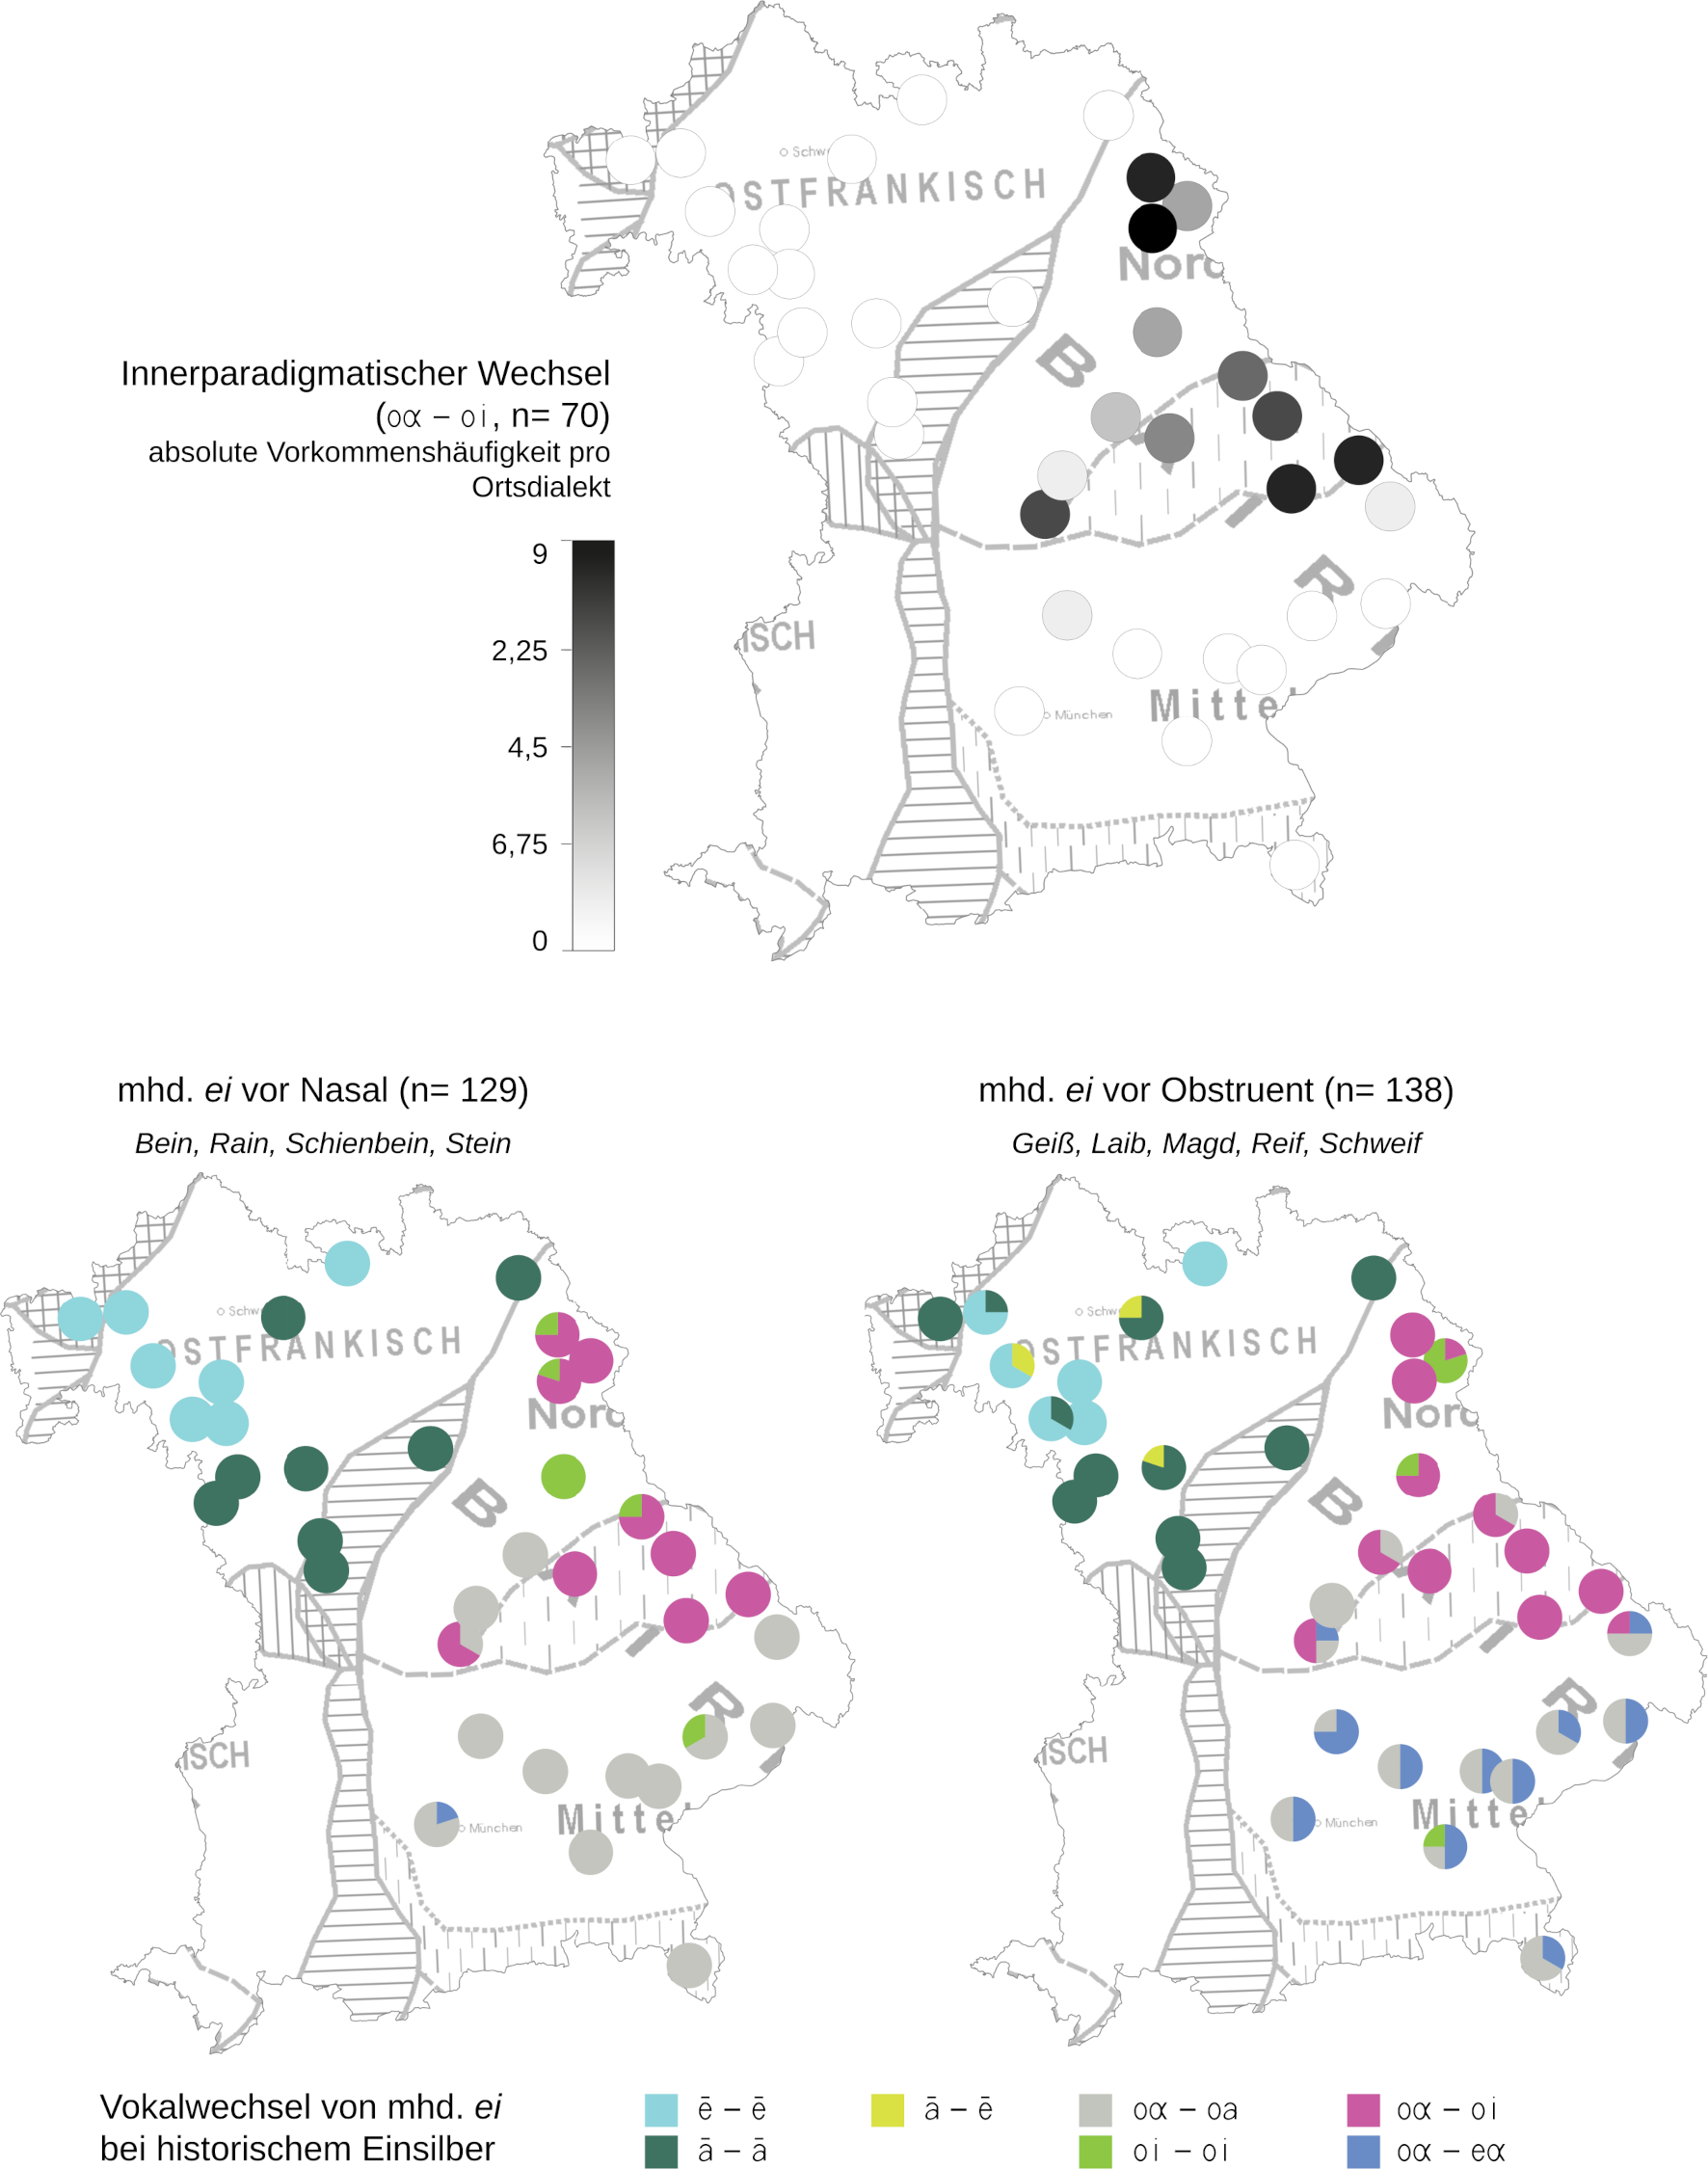
\includegraphics[width=\textwidth]{figures/Karte5.png}
\caption{Häufigkeitsverteilung der Vokalwechsel von mhd. \textit{ei} bei historischen Einsilbern und Chloroplethkarte mit absoluter Vorkommenshäufigkeit des \textit{oα-oi}{}-Wechsels}
\label{map:5}
\end{map}

Dieser innerparadigmatische Wechsel findet sich in Flexionsformen und Wortbildungen, z.\,B. Sg. \teuthoo{lo<.A}{lôͅα} -- Pl. \teuthoo{lo<i}{lôi} -- Dim. \teuthoo{lo.<iw@l@}{lôͅiw̥l̥} (‚Laib‘, nordbair.-mittelbair. Grafenkirchen). „Umlautähnlich“ ist der Kontrast der Vokalqualität nach \citet[66]{Rowley1997} deshalb, weil der Vokalwechsel zwar dem Umlaut ähnelt, aber keine Korrelation der Zungenhöhe besteht (vgl. \sectref{sec:7.1.2.1.1}). Im UG gibt es neben diesem Wechsel ohne Korrelation der Zungenhöhe Belege für einen Diphthongwechsel mit Zungenhöhenkorrelation, d.\,h. einen analogen Umlaut \teuthoo{oA}{oα} -- \teuthoo{eA}{eα} anstelle des lauthistorischen Diphthongs \teuthoo{oi}{oi}. Im nördlichen Nordbair. ist dieser Diphthongwechsel v.\,a. in Komparativformen belegt, \citet[66]{Rowley1997} führt die Komparativform \teuthoo{weac!a}{weaꭖa} ‚weicher‘ neben der lautgesetzlichen Realisierung \teuthoo{woic!a}{woiꭖa} an.\footnote{Vgl. auch \citet[§75.1]{Kollmer1987}, \citet[§75c6]{Micko1930}, \citet[96]{Roth1940}, \citet[§56.4]{Schießl1914}. Im mittelbair. Dialekt der Hallertau ist der analoge Umlaut in Komparativformen „keineswegs obligatorisch“, \textit{wɔ\textsuperscript{a}}\textit{ha} ist neben \textit{wɛ\textsuperscript{a}}\textit{ha} ‚weicher‘ belegt \citep[167]{Zehetner1978}. \citet[168]{Zehetner1978} bietet daneben Belege für den analogen Umlaut in Wortbildungen, z.\,B. /brɛ\textsuperscript{a}dn/ ‚Breite‘ zu /brɔ\textsuperscript{a}d/ ‚breit‘, /sɔ\textsuperscript{a}h/ ‚Urin‘ und /sɛ\textsuperscript{a}hin/ ‚nach Urin riechen‘, aber /gɔ\textsuperscript{a}s/ ‚Geiß‘, /gɔ\textsuperscript{a}sln/ ‚nach Geiß riechen‘.}  In den BSA-Daten findet sich der analoge Umlaut mit Zungenhöhenkorrelation (\teuthoo{eA}{eα}) vor allem in den mittelbair. Ortsdialekten bei den Lexemen \textit{Schweif}, z.\,T. \textit{Reif} und \textit{Geiß}. Der einzige Beleg des Wechsels \teuthoo{oA}{oα} -- \teuthoo{eA}{eα} vor Nasal in \textit{Stein} im mittelbair. Pasing (\teuthoo{s\#de<A<nA}{šdêα̂nα} neben \teuthoo{s\#do>+A+}{šdỗα̃}, \teuthoo{s\#do>+A+nA}{šdỗα̃nα}) ist nach \citet[168]{Zehetner1978} „nicht eigentlich ländlich, sondern anscheinend münchnerischer Provenienz“ (vgl. \citealt[Karte 78]{SOB4}). Im Dialekt von München und im westmittelbair. Eisenhofen ist dieses analoge Umlautmuster auch bei mhd. \textit{î} in \textit{Streifen} (mhd. \textit{strîfe}) belegt: \teuthoo{s\#dro.2Af}{šdrōͅαf} -- \teuthoo{s\#tre.Af}{štreͅαf} (\citealt[79]{Wittmann1943}, vgl. \citealt[44]{White1966}).\footnote{Im Dialekt von Eisenhofen ist das Umlautmuster \teuthoo{oA}{oα} -- \teuthoo{eA}{eα} bei Maskulina und Neutra stark besetzt, da es -- nach \citet[44]{White1966} -- die rezente Entsprechung von mhd. \textit{ô}/\textit{œ} (\teuthoo{flo.ax}{f‌loͅax} -- \teuthoo{fle.ax}{f‌leͅax} ‚Floh‘) und von mhd. \textit{o}/\textit{ö} vor /r/ (\teuthoo{kho.a«r»b}{khoͅa(r)b} -- \teuthoo{khe.a«r»b}{kheͅa(r)b} ‚Korb‘) bildet. Der analoge Umlaut bei mhd. \textit{ei} in \textit{Streifen} und \textit{Schweif} entspricht diesem Muster. Neben Belegen eines analogen Umlauts \teuthoo{oA}{oα} -- \teuthoo{eA}{eα} in Plural- und Komparativformen (\teuthoo{s\#wo.2Af}{šwōͅαf} -- \teuthoo{s\#weAff}{šweαff} ‚Schweif‘, \teuthoo{bro.Ad}{broͅαd} -- \teuthoo{bre2AdA}{brēαdα} ‚breit‘) berichtet \citet[85]{Grundler1951} für das mittelbair. Erding außerdem von semantischen Unterschieden bei Formen ohne bzw. mit analogem Umlaut: \teuthoo{bro2.Adn}{brōͅαdn} ‚breiter Acker‘, \teuthoo{bre2Adn}{brēαdn} ‚Breite (Maßbezeichnung)‘ für mhd. \textit{breite}.}

Die Entsprechung von mhd. \textit{ei} ist im Verbreitungsgebiet vor Nasal z.\,T. anders verlaufen als vor Obstruent, weshalb die beiden lautlichen Umgebungen in \mapref{map:5} getrennt behandelt wurden (vgl. \citealt[Karten 20--22]{Gütter1971}, \citealt[56--59]{RennKönig2006}, \citealt[66 und Karte 12]{Rowley1997}). An der Raumbildung der Karte lässt sich dabei die unterschiedliche Normalentwicklung im Ofr. und im Bair. nachvollziehen. In den ofr. Ortsdialekten finden sich die monophthongischen Realisierungen \teuthoo{e2}{ē} oder \teuthoo{a2}{ạ̄}, während mhd. \textit{ei} in den bair. Dialekten diphthongisch realisiert wird. Interessant an den ofr. Daten ist, dass es auch hier Belege für einen analogen Umlaut gibt (einzig bei dem Lexem \textit{Reif}, Typ \teuthoo{ra2v}{rāv} -- \teuthoo{re2v}{rēv}).\footnote{In Erlabrunn gibt es zudem einen Einzelbeleg für eine Alternation der Vokalqualität mittels Entrundung des Stammvokals bei gleichzeitiger Kürzung: \teuthoo{ro"?:v5}{rȫ{\doubleogonek}v̩} -- \teuthoo{re?v5}{rëv̩} (‚Reif‘).}

Im bair. Teil des UGs gibt es eine Zweiteilung. Im Nordbair. und im nordbair.-mittelbair. Übergangsgebiet überwiegt die innerparadigmatische Alternation \teuthoo{oA}{oα} -- \teuthoo{oi}{oi}, während im größten Teil der mittelbair. Tiefenbohrungspunkte die Realisierung von mhd. \textit{ei} ohne innerparadigmatischen Wechsel überwiegt (\teuthoo{oA}{oα} -- \teuthoo{oA}{oα}). Der Diphthong \teuthoo{oA}{oα} entspricht hier der mittelbair. Normalentwicklung von mhd. \textit{ei} (vgl. \citealt[§20h]{Kranzmayer1956}). Auch im Nordbair. sowie im nordbair.-mittelbair. Übergangsgebiet gibt es Belege für Formen ohne innerparadigmatischen Wechsel, jedoch ist dieser innerparadigmatische Ausgleich lexemweise zu \teuthoo{oi}{oi} erfolgt, im gesamten UG etwa bei \textit{Rain} (vgl. \citealt[441]{Götz1987}, \citealt[§75]{Micko1930}). Bemerkenswert ist, dass die Ausdifferenzierung der rezenten Entsprechungen von mhd. \textit{ei} relativ jung zu sein scheint. \citet[§14]{Micko-Repp1933} gibt den lautgesetzlichen \teuthoo{oA}{oα}-\teuthoo{oi}{oi}-Wechsel als Variante der älteren Generation an, die im mittelbair. Wadetstift neben Formen ohne innerparadigmatischen Wechsel (\teuthoo{oi}{oi} -- \teuthoo{oi}{oi}) belegt ist; der Wechsel \teuthoo{oA}{oα} -- \teuthoo{eA}{eα} sei als „jüngste Erscheinung“ im Basisdialekt noch selten.


\begin{map}
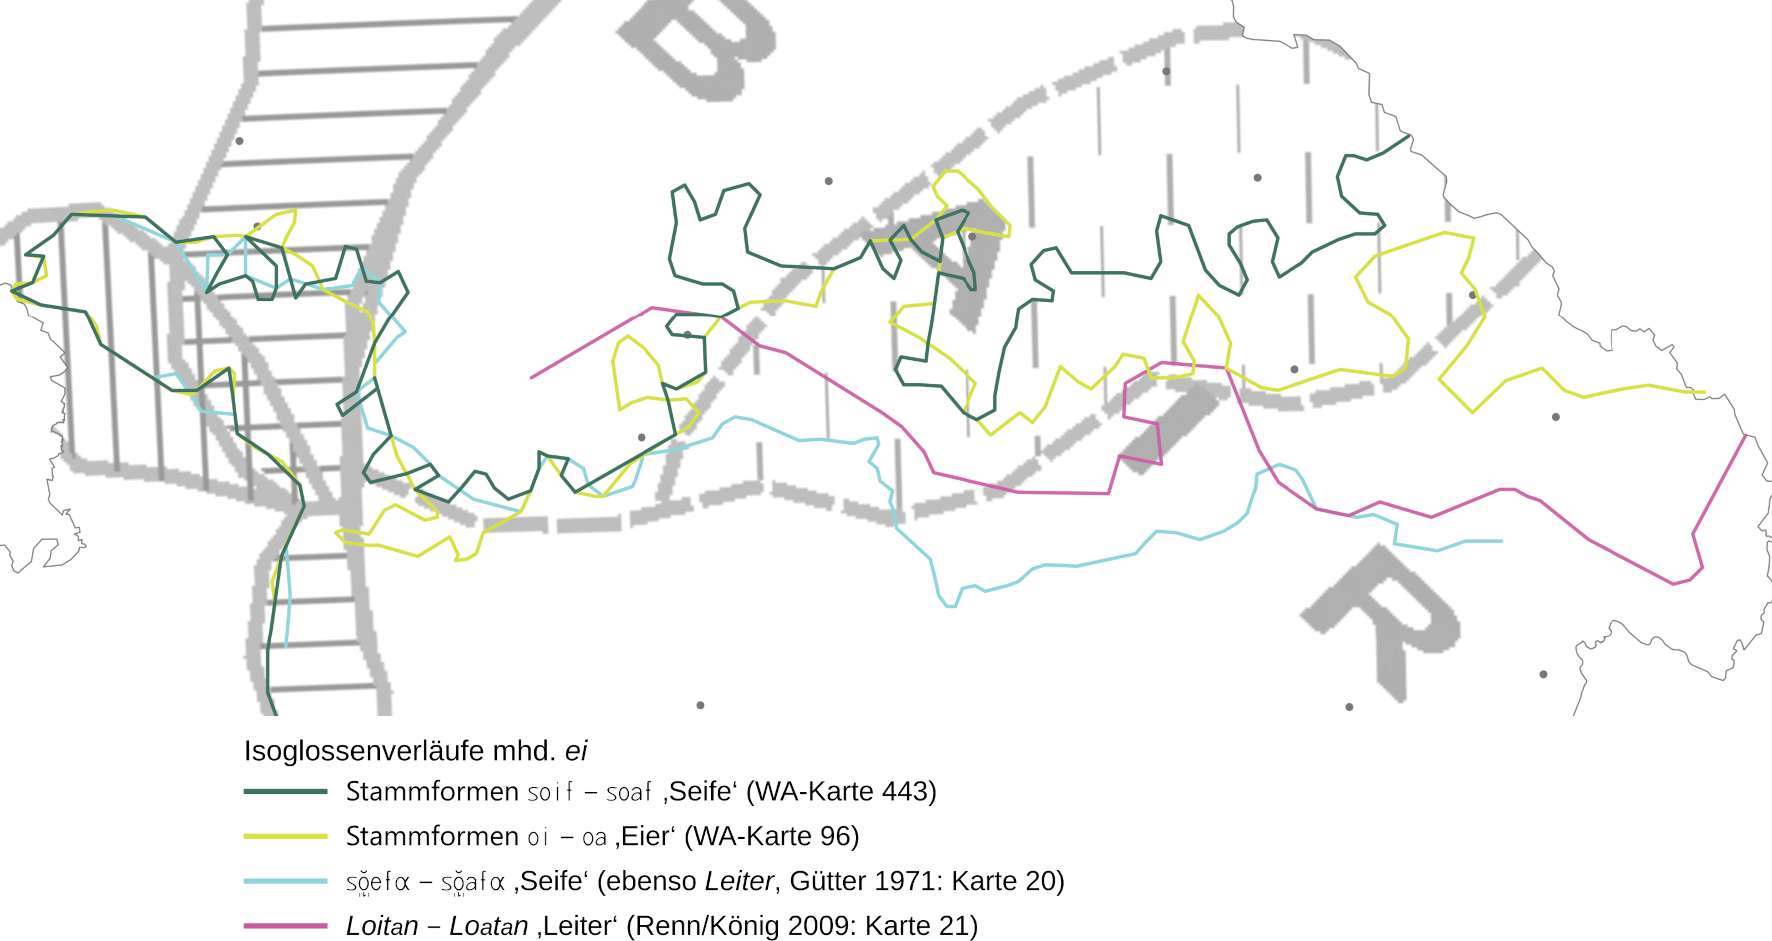
\includegraphics[width=\textwidth]{figures/Karte6.png}
\caption{Lexemspezifische Isoglossenverläufe von mhd. \textit{ei} im nordbairisch-mittelbairischen Übergangsgebiet}
\label{map:6}
\end{map}

Ein Vergleich mit den relevanten Wenker-Karten\footnote{Im \textit{Sprachatlas des Deutschen Reich} sind drei Lexeme mit historischen Mehrsilbern kartiert (\textit{Eier}, \textit{Kleider}, \textit{Seife}). Die \citealt{WA}-Karte \textit{Kleider} (Akk.Pl.) ist dabei nur bedingt aufschlussreich, da im größten Teil des Bair. das Heteronym \textit{Gewand} verbreitet ist.} zeigt, dass auch im südlichen Nordbair., d.\,h. in jenem Areal, für das die Leitform \teuthoo{oi}{oi} gilt, Formen mit dem Diphthong \teuthoo{oA}{oα} in der Stammform (\textit{kload}{}-, \textit{soaf}{}-)\footnote{\citealt{WA}-Karte 444 (\textit{Seife}, Akk.Sg.fem.) zeigt, dass \textit{Seife} in diesem Gebiet auch synchron zweisilbig in der \textit{n}{}-erweiterten Form (und nicht etwa in der einsilbigen apokopierten Form) realisiert wird.} belegt sind. Damit ist auch im Wenker-Material eine Varianz zwischen Vokalwechsel und innerparadigmatischem Ausgleich (nach mittelbair. Normalentwicklung) zu finden. Gleichzeitig zeigen die Isoglossenverläufe, dass die Realisierung des Diphthongs in diesem Übergangsgebiet lexemspezifisch zu sein scheint (\mapref{map:6}).

Aufgrund der geringen Anzahl der abgefragten Lexeme für die jeweilige phonologische Umgebung von mhd. \textit{ei} vor Nasal vs. Obstruent ist es schwierig, über lexemspezifische Entwicklungen hinaus zu generalisieren. Die areale Verteilung der Diphthongwechsel ergibt in der Tendenz für die nordbair. Ortsdialekte die umlautähnlichen Wechsel \teuthoo{oA}{oα} -- \teuthoo{oi}{oi} sowie den Typus \teuthoo{oi}{oi} -- \teuthoo{oi}{oi} ohne Alternanz, während in den mittelbair. Orten der Typus \teuthoo{oA}{oα} -- \teuthoo{oA}{oα} (sowie vereinzelt \teuthoo{oi}{oi} -- \teuthoo{oi}{oi}) und die Alternation mit Zungenhöhenkorrelation \teuthoo{oA}{oα} -- \teuthoo{eA}{eα} belegt ist. Im nordbair.-mittelbair. Übergangsgebiet sind neben dem \teuthoo{oA}{oα}-\teuthoo{oi}{oi}-Wechsel beide Ausgleichsvarianten (\teuthoo{oA}{oα} -- \teuthoo{oA}{oα} und \teuthoo{oi}{oi} -- \teuthoo{oi}{oi}) zu finden. Damit sind die innerparadigmatischen Diphthongwechsel ein spezifisches Phänomen des Nordbair. und des nordbair.-mittelbair. Übergangsgebiets, während der analoge Umlaut \teuthoo{oA}{oα} -- \teuthoo{eA}{eα} im Mittelbair. gilt, sich aber nach Norden hin auszudehnen scheint. Laut \citet[167]{Zehetner1978} finden sich diese \teuthoo{oA}{oα}-\teuthoo{eA}{eα}-Formen in der mittelbair. Hallertau, nicht aber in dem Gebiet nördlich bis zur Donau („Donauland“), da man dort der Markierung der Pluralinformation durch analogen Umlaut aufgrund der lautgesetzlichen \teuthoo{oA}{oα}-\teuthoo{oi}{oi}-Alternation nicht „bedurfte“. Während sich in den vorliegenden Daten ein einzelner Beleg der \teuthoo{oA}{oα}-\teuthoo{eA}{eα}-Alternation im südlichen Nordbair. in Oberdolling (\teuthoo{ro4Af}{rọαf} -- \teuthoo{re.Af,}{reͅαf͓} ‚Reif‘) findet, zeigen die BSA-Karten zur Pluralmarkierung von \textit{Geiß} demgegenüber ein relativ geschlossenes Gebiet des Typs \teuthoo{go<As}{ɡôαs} -- \teuthoo{geAS}{ɡeᾳʃ}, das die Hallertau und auch das „Donauland“ nördlich davon umfasst (vgl. \citealt[Karte 8]{SOB4}, \citealt[Karte 89/90]{SNiB7}).\largerpage

Insgesamt scheint die Realisierung von mhd. \textit{ei} mit oder ohne Vokalwechsel in den untersuchten Ortsdialekten aber stark lexemspezifisch zu sein. Aus flexionsmorphologischer Perspektive führen beide Realisierungsvarianten des innerparadigmatischen Vokalwechsel (\teuthoo{oA}{oα} -- \teuthoo{oi}{oi} bzw. \teuthoo{oA}{oα} -- \teuthoo{eA}{eα}) zu differenten Singular- und Pluralformen. In den Singular- und Pluralformen ohne innerparadigmatische Alternation wird der Plural nicht modulativ in Form eines (umlautähnlichen oder analogen Umlaut-)Vokalwechsels, sondern mittels anderer Pluralmarkierungsstrategien respektive Nullplural gebildet. \citet{Wildfeuer2001} beschreibt in seiner Apparent-time-Studie dreier mittelbair. Sprechergruppen einen Wandel hin zu einer kumulativen Markierung des Plurals von \textit{Stein}. In der älteren Sprechergruppe ist der Diphthongwechsel von mhd. \textit{ei} im Sg. [õα] zu Pl. [ãi] mit 80\,\% belegt, bei der mittleren Sprechergruppe mit 70\,\%, während die jüngere Gruppe den Plural von \textit{Stein} nur zu 30\,\% rein modulativ mit Diphthongwechsel bildet und in der Mehrzahl (70\,\%) die „Maximalmarkierung“, d.\,h. den modulativ-additiven Plural des Typs \textit{šdõα} -- \textit{šdãinα}, verwendet \citep[188]{Wildfeuer2001}.

Als Pluralmarkierungsverfahren funktionalisiert und produktiv ist der Diph\-thong\-wech\-sel \teuthoo{oA}{oα} -- \teuthoo{oi}{oi} da, wo er unabhängig von der phonologischen Umgebung der historischen Ein- vs. Mehrsilbigkeit in (ehemals) zweisilbigen Substantiven erscheint (vgl. \tabref{tab:21}): \teuthoo{gmo+A}{ɡmõα} -- \teuthoo{gmoi}{ɡmoi} ‚Gemeinde‘ (nordbair.-mittelbair. Bernhardswald), \teuthoo{so4<AfA}{sộαfα} -- \teuthoo{so4<e4f,An}{sộẹf͓αn} ‚Seife‘ (nordbair. Riedenburg), \teuthoo{s\#po<AH}{špôαhͯ} -- \teuthoo{s\#po<EHAn}{špôəhͯαn} ‚Speiche‘ (mittelbair. Wolfersdorf), \teuthoo{o<AHA}{ôαhͯα} -- \teuthoo{o4<eXAn}{ộeꭗαn} ‚Eiche‘ (nordbair. Oberdolling).

\begin{table}
\begin{tabularx}{\textwidth}{QQ}
\lsptoprule
Historische Einsilber & Historische Mehrsilber\\
\midrule
\textit{Bein, Ei}, \textit{Geiß}, \textit{Laib}, \textit{Magd/Maid,}\footnote{Mhd. \textit{ege} in \textit{megetlîn} wird zu \textit{ei} kontrahiert (ebenso in \textit{getregede} ‚Getreide‘), kontrahiertes \textit{ei} entwickelt sich in der Folge in den untersuchten Dialekten analog zu mhd. \textit{ei}, z.\,B. \teuthoo{mo.2i\textsuperscript{d}l@}{mōͅi\textsuperscript{d}l̥}, \teuthoo{d5ro2.i}{d̩rōͅi} im nordbair. Kallmünz \citep[441]{Götz1987} vs. \textit{drɔ\textsuperscript{a}}\textit{d} in der mittelbair. Hallertau (\citealt[158]{Zehetner1978}, vgl. \citealt[32]{Förster1912/13}, \citealt[§81]{Gebhardt1907}, \citealt[83]{Grundler1951}, \citealt[§75d]{Micko1930}.} \textit{Rain, Reif(en)}, \textit{Schweif}, \textit{Seil}, \textit{Stein}  & \textit{Breite}\footnote{nur SMF} \textit{Eiche}, (\textit{Ge}{}-)\textit{Leise}, \textit{Gemeinde}, \textit{Seife}, \textit{Speiche}\\
\lspbottomrule
\end{tabularx}
\caption{Lexeme mit mhd. \textit{ei} als Stammvokal im Korpus}
\label{tab:21}
\end{table}


\subsubsubsection{Wechsel der Zungenhöhe}\label{sec:7.1.2.1.3}\largerpage[2]
Im UG sind mhd. \textit{e} und \textit{ö} in Dehnung teilweise zu \textit{ī} gehoben worden, im östlichen Ofr. und im nördlichen Nordbair. werden sie diphthongisch als \teuthoo{I2A}{ı̄α} realisiert (vgl. \sectref{sec:7.1.2.1.1}).{\interfootnotelinepenalty=10000\footnote{Vgl. \citet[Karte 3]{Gütter1971}, \citet[4d]{Kranzmayer1956}, \citet[73--74 und Karte 15]{Rowley1997}, \citet[121--125 und Karte 22]{Steger1968}, \citealt[75]{SMF3}, \citet[1110]{Wiesinger1983c}. Daneben wurde in der Parallelreihe mhd. \textit{e-ö-o} auch mhd. \textit{o} zu \textit{ū} gehoben (vgl. \citealt[Karte 4]{Gütter1971}, \citealt[73 und Karte 15]{Rowley1997}).}} Die Dehnung des Stammvokals ist im Rahmen der Einsilberdehnung nur in der Singularform, nicht aber in der additiven und damit zweisilbigen Pluralform eingetreten, weshalb in jenen Ortsdialekten, in denen mhd. \textit{e} und \textit{ö} in Dehnung gehoben wurden, innerparadigmatische Alternationen zwischen gehobenem Vokal in der Singularform und im Plural mhd. \textit{e} bzw. \textit{ö} in Normalentwicklung erscheinen (mhd. \textit{ö} nur in einer Form mit sogenannter Markiertheitsumkehrung im ofr.-hess Wiesthal, vgl. \tabref{tab:22}).
Die Alternation besteht damit in einem lautgesetzlich entstandenen Wechsel der Zungenhöhe bei zwei Palatalvokalen. Bemerkenswert sind hier die Belege für \textit{Erle} und \textit{Kerze} im Nord- und Mittelbair., da der Wechsel der Zungenhöhe nicht bei historischen Ein-, sondern Zweisilbern erscheint und damit nicht lautgesetzlich ist.

Daneben gibt es eine weitere Form eines Wechsels der Zungenhöhe zwischen geschlossenem \teuthoo{e24}{ẹ̄} und offenem \teuthoo{e.}{eͅ}, den \citet[116--117]{Rowley1997} für das nördliche Nordbair. anführt und der sich in den vorliegenden Daten im nordbair. Windischeschenbach und Nabburg und daneben im ofr.-nordbair. Übergangsgebiet (Tiefenbohrungspunkte Pfofeld\footnote{Karten 25/26 (mhd. \textit{e} in \textit{Zähne}, \textit{Blätter}) und 28 (mhd. \textit{ö} in \textit{Vögel}) in \citet{Kollmann1961} zeigen die Isoglossenverläufe der Hebung von mhd. \textit{e}, \textit{ö} in Dehnung im ofr.-nordbair. Übergangsgebiet und dass diese im Tiefenbohrungspunkt Pfofeld ebenfalls teilweise erfolgt ist, vgl. die Formen in den eigenen Daten: \teuthoo{vu42gJ}{vụ̄ɡ{\lkreis}} -- \teuthoo{vi4"gJ}{vị̄ɡ{\lkreis}} -- \teuthoo{ve.hAl.A}{veͅhαlͅα} ‚Vogel‘, aber \teuthoo{dsu42}{dsụ̄} -- \teuthoo{dse42}{dsẹ̄} ‚Zahn‘ (vgl. \citealt[22--24]{Kollmann1961} sowie \citealt[Karte 33/34]{Brendel1962}, \citealt[§12 und Karte 3]{Kaußler1962}, \citealt[Karte 22]{Kopp1959}).} und Kirchensittenbach) findet (vgl. \citealt[§65]{Kollmer1985}).

Ortsdialektspezifisch ist daneben die Senkung von mhd. \textit{i} in historischen Zweisilbern und die resultierende innerparadigmatische Alternation in Wiesthal im ofr.-hess. Übergangsgebiet (vgl. \citealt[1108]{Wiesinger1983c}).

\begin{table}
\small
\begin{tabularx}{\textwidth}{llllQ}
\lsptoprule
& {Singular} & {Plural} & &\\
\midrule
\makecell[tl]{{mhd. \textit{ë},}\\
{mhd. \textit{e}}} & \teuthoo{brI9."d}{brı\klammeruntenpost{}̄ͅd} & \teuthoo{bre4dE}{brẹdə} & \multicolumn{2}{>{\raggedright\arraybackslash}p{.53\textwidth}}{‚Brett‘ (ofr. Burgbernheim, daneben ofr.-nordbair. Pfofeld)}\\
\tablevspace
& \teuthoo{vôe?e\$d}{v{\aufstrih}ëe̤d} & \teuthoo{v\%ôe?i.dA}{v͈{\aufstrih}ëiͅdα} & \multicolumn{2}{>{\raggedright\arraybackslash}p{.53\textwidth}}{‚Feld‘ (nordbair. Oberdolling, daneben ofr.-nordbair. Kirchensittenbach)}\\
\tablevspace
& \teuthoo{ni94"s\#d}{ni\klammeruntenpost{}̣̄šd} & \teuthoo{ne.s\#dA}{neͅšdα} & \multicolumn{2}{>{\raggedright\arraybackslash}p{.53\textwidth}}{‚Nest‘ (ofr.-nordbair. Mitteleschenbach, daneben ofr. Burgbernheim und Pfofeld, nordbair. Groschlattengrün, Tirschenreuth und Windischeschenbach, vgl. \citealt[Karte 40]{SUF3})}\\
\tablevspace
& \teuthoo{vle42g}{vlẹ̄ɡ} & \teuthoo{vle.gá\_}{vleͅɡ͈ʰ} & \multicolumn{2}{>{\raggedright\arraybackslash}p{.53\textwidth}}{‚Fleck‘ (ofr.-nordbair. Pfofeld, vgl. \citealt[69]{SNOB1})}\\
\tablevspace
& \teuthoo{gðNec1d}{ɡ̩ŋeX\⚬d} & \teuthoo{gNe.c1t}{ɡŋeͅX\⚬t} & \multicolumn{2}{>{\raggedright\arraybackslash}p{.53\textwidth}}{‚Knecht‘ (nordbair. Nabburg, daneben ofr.-nordbair. Pfofeld, nordbair. Windischeschenbach)} \\
\tablevspace
& \teuthoo{i.“A2l}{īͅᾱl} & \teuthoo{e\$Aln}{e̤αln} & \multicolumn{2}{>{\raggedright\arraybackslash}p{.53\textwidth}}{‚Erle‘ (mittelbair. Neukirchen am Inn, daneben mittelbair. Waldhof)}\\
\tablevspace
& \teuthoo{g\_iEtSn@}{ɡʰiətʃn̥} & \teuthoo{g\_e.EtSn@}{ɡʰeͅətʃn̥} & \multicolumn{2}{>{\raggedright\arraybackslash}p{.53\textwidth}}{‚Kerze‘ (nordbair. Groschlattengrün, daneben mittelbair. Inning am Holz und Neukirchen am Inn)}\\
\tablevspace
{mhd. \textit{i}} & \teuthoo{vi“s\#}{vīš} & \teuthoo{ve94s\#}{ve\klammeruntenpost{}̣̄š} & {‚Fisch‘} & \multirow[t]{4}{=}{(ofr.-hess.-Wiesthal, vgl. \citealt[Karte 4]{SUF1}, \citealt{WA}-Karte 449 ‚Tische‘)}\\
& \teuthoo{gri“v5}{ɡrīv̩} & \teuthoo{gre4v5}{ɡrẹv̩} & {‚Griff‘} & \\
& \teuthoo{s\#di“c}{šdīX} & \teuthoo{s\#deX}{šdeꭗ} & {‚Stich‘} & \\
& \teuthoo{di“s\#}{dīš} & \teuthoo{dswe2}{dswē} \teuthoo{des#}{deš} & {‚Tisch‘} & \\
& \teuthoo{wi“E.d}{wīəͅd} & \teuthoo{we4d5\_}{wẹd̩ʰ} & \multicolumn{2}{>{\raggedright\arraybackslash}p{.53\textwidth}}{‚Wirt‘ (ofr. Erlabrunn, daneben ofr. Ochsenfurt, vgl. \citealt[Karte 16]{SUF1})}\\
\tablevspace
{mhd. \textit{ö}} & \makecell[tl]{\teuthoo{dsi.“bv5}{dsīͅbv̩}\\(neben\\\teuthoo{dse\$2bv}{dsē̤bv})} & \makecell[tl](\teuthoo{di la.NE dse4bv5}{di laͅŋə dsẹbv̩}) & \multicolumn{2}{>{\raggedright\arraybackslash}p{.53\textwidth}}{‚Zopf‘ (ofr.-hess.-Wiesthal)}\\
\lspbottomrule
\end{tabularx}
\caption{Belege von innerparadigmatischem Wechsel der Zungenhöhe im UG ($n=26$)}
\label{tab:22}
\end{table}

\subsubsection{Kontraste der Vokalquantität}
\label{sec:7.1.2.2}
Innerparadigmatische Kontraste der Quantität des Stammvokals können als Numerusmarker funktionalisiert sein. Die Pluralmarkierung findet dabei (wie auch die Modulation der Vokalqualität) an einer „symbolverdächtigen Stelle des Wortes“ \citep[283]{Harnisch1994a} statt (anders als beispielsweise Konsonantenelisionen oder -fortisierungen im Stammauslaut, vgl. \sectref{sec:7.1.2.3}). Kürzungen der Vokalquantität werden hier nicht als Form eines subtraktiven Plurals, sondern als Modulationen der Vokalquantität klassifiziert (vgl. \citealt[25]{Birkenes2014}, \citealt[584]{Dressler2000}, anders \citealt{Nübling2006} für das Luxemburgische).

Im UG erfolgte phonologischer Wandel der Vokalquantität durch Dehnung in offener Tonsilbe, durch Dehnung von mhd. Einsilbern mit betontem Kurzvokal sowie durch Kürzung historischer Dreisilber.\footnote{Siehe hierzu \citet[§E33 und §34k]{Kranzmayer1956}, \citet[69--73]{Rowley1997}, \citet[181--189]{Schirmunski1962}, \citet{Seiler2009}, \citet[35--41]{Steger1968}, \citet[1091--1094]{Wiesinger1983a}.} Laut \citet[§34k.1]{Kranzmayer1956} entspringen sämtliche historische Veränderungen der Vokalquantität im UG dem „Bemühen, die Wortkörper unabhängig von ihrer Silbenzahl gleich lang zu gestalten“ (vgl. \citealt[12]{Kollmer1949}). Einen ähnlichen Erklärungsansatz der Quantitätsverhältnisse im Ofr. und Bair. bietet die Morentheorie (vgl. einführend \citealt[1071--1074]{Auer1989} sowie \citealt{Auer1991}): Das minimale Wort besteht in Dialekten, die Einsilberdehnung durchgeführt haben, aus einer zweimorigen Silbenstruktur (vgl. \citealt[254--260]{Seiler2009} sowie \sectref{sec:7.1.2.3.1}). Um diese zu erfüllen, wird der kurze (einmorige) Vokal zu einem langen (zweimorigen) Vokal gedehnt, der auslautende Konsonant ist nicht-morenwertig.

Werden historische Einsilber synchron mit Kurzvokal realisiert, so kann dies laut \citet[70]{Rowley1997} das Ergebnis von standardsprachlichem Einfluss oder von innerparadigmatischem Ausgleich sein, \citet[132--133]{Schübel1955} führt für den ofr. Dialekt Stadtsteinachs zudem die auf den Stammvokal folgende Konsonantenverbindung sowie die Gebrauchsfrequenz als mögliche Einflussfaktoren an. \citet[§34k5]{Kranzmayer1956} zufolge ist die Einsilberdehnung im Nordbair. und Ofr. „am besten bewahrt“, doch sind die lautgesetzlichen Quantitätsverhältnisse im Ofr. laut \citet[71]{Rowley1997} durch innerparadigmatischen Ausgleich „mancherorts stark verwischt“ (vgl. \citealt[70--71]{Heilig1898}, \citealt[1]{Heinebrodt1963}, \citealt[Karte 22]{Kranzmayer1956}). Erhalten sind die Quantitätskontraste in einem Teil des Ofr. (Bayreuther, Bamberger und Erlanger Raum) dagegen systematisch in Kombination mit Kontrasten der Vokalqualität, etwa bei einem Wechsel der Zungenhöhe wie in \teuthoo{vle2g}{vlēg} -- \teuthoo{vle.g}{vleͅɡ} ‚Fleck‘ \citep[194]{Rowley1997}.

Aus flexionsmorphologischer Perspektive sind die phonologischen Prozesse, die die Vokalquantität betreffen, dann relevant, wenn innerparadigmatische Alternationen zwischen Kurz- und Langvokal entstehen, wie es infolge der Einsilberdehnung der Fall ist. Der Stammvokal der einsilbigen Singularform wurde gedehnt, der Stammvokal in geschlossener Tonsilbe der zweisilbigen (additiven) Pluralform und der Diminutivform blieben kurz, z.\,B. \teuthoo{blo942d\_}{blo\klammeruntenpost{}̣̄dʰ} -- \teuthoo{ble):dA}{ble\klammeruntenpost{}{\doubleogonek}dα} ‚Blatt‘ (ofr.-nordbair. Mitteleschenbach), \teuthoo{vo2s5}{vōs̩} -- \teuthoo{ve.s4Er}{veͅṣər} -- Dim. \teuthoo{ve.sla}{veͅsla} ‚Fass‘ (ofr. Hallerstein).\footnote{Quantitätskontraste durch Einsilberdehnung und erhaltene Kürze aufgrund von Mehrsilbigkeit erscheint -- wie die Diminutivformen zeigen -- nicht nur innerhalb von Flexionsparadigmen, sondern auch bei Wortbildungen, wie die ofr. Beispiele von \citet[132]{Schübel1955} illustrieren: \teuthoo{wI2Ed}{wı̄əd} -- \teuthoo{wedA}{wedα} -- \teuthoo{wedshaus}{wedshaus} ‚Wirt -- Wirtin -- Wirtshaus‘, \teuthoo{gnu2ofb}{ɡnūofb} -- \teuthoo{gnobflox}{ɡnobf‌lox} -- \teuthoo{gno?bflA}{ɡnöbf‌lα} ‚Knopf -- Knopfloch -- Knöpfchen‘.}  Wies die zweisilbige Pluralform eine offene Tonsilbe auf, trat lautgesetzliche Dehnung in offener Tonsilbe ein, z.\,B. \teuthoo{ro.2d5\_}{rōͅd̩ʰ} -- \teuthoo{re9.2dE.}{re\klammeruntenpost{}̄ͅdəͅ} -- Dim. \teuthoo{re.2dJA94.}{rēͅd{\lkreis}α\klammeruntenpost{}̣ͅ} ‚Rad‘ (ofr. Burgbernheim), \teuthoo{glo.2s}{ɡlōͅs} -- \teuthoo{gle.2sA}{ɡlēͅsα} -- Dim. \teuthoo{gla42sl}{ɡlạ̄sl} ‚Glas‘ (mittelbair. Kirchensur). Bei mhd. Substantiven mit Schwa als Pluralmarker entstanden infolge eines zweiten (nachfolgenden)\footnote{Hierzu führt \citet[§266]{Heilig1898} aus (vgl. \citealt[48]{Roth1940}): „Diese Formen [d.\,h. Formen mit innerparadigmatischem Quantitätenkontrast des Typs vīš -- viš ‚Fisch‘, GN] beweisen, daß nach dem Abfall des \textit{e} die Dehnung der einsilbigen Wörter bereits abgeschlossen gewesen sein muss.“}  phonologischen Prozesses, der Apokope, rein stammaffizierende Flexionsformen des Typs \teuthoo{vi“s\#}{vīš} -- \teuthoo{vI3s\#5}{vı̆š̩} ‚Fisch‘ (nordbair. Groschlattengrün). Die phonologische Umgebung der Einsilberdehnung (bestehend im Kontrast zur zweisilbigen Pluralform) war nicht mehr transparent (vgl. \citealt[188]{Seiler2008}).

\begin{table}
\small
\begin{tabularx}{\textwidth}{lQQQ>{\raggedright\arraybackslash}p{.1\textwidth}>{\raggedright\arraybackslash}p{.25\textwidth}}
\lsptoprule
\makecell[tl]{{Quantitäts-}\\{muster}} & {Singular} & {Plural} & {Diminutiv} & &\\
\midrule
{(a) K -- K} -- K & \teuthoo{dê}{d{\burgereshwa}} \teuthoo{qågê}{ʔ{\burgeroalpha}ɡ{\burgereshwa}} & \teuthoo{di}{di} \teuthoo{qa94gê}{ʔa\klammeruntenpost{}̣ɡ{\burgereshwa}} & \teuthoo{Aq}{αʔ} \teuthoo{a94gêlA}{a\klammeruntenpost{}̣ɡ{\burgereshwa}lα} & \multicolumn{2}{>{\raggedright\arraybackslash}p{.35\textwidth}}{‚Acker‘ (ofr. Ahorn)}\\
 &   \teuthoo{do4xd}{dọxd} & \teuthoo{de?cd}{dëXd} & \teuthoo{de?cdlA}{dëXdlα} & \multicolumn{2}{>{\raggedright\arraybackslash}p{.35\textwidth}}{‚Docht‘ (ofr. Hüttenheim)}\\
 \tablevspace
 {(b) L -- L} -- L & \teuthoo{go.2wl@}{ɡōͅwl̥} & \teuthoo{go.2wl@}{ɡōͅwl̥} & \teuthoo{go"?.wElE}{ɡȫͅwələ} & \multicolumn{2}{>{\raggedright\arraybackslash}p{.3\textwidth}}{‚Gabel‘ (ofr. Gemünden am Main)}\\
 &  \teuthoo{glo.2s}{ɡlōͅs} & \teuthoo{gle.2sA}{ɡlēͅsα} & \teuthoo{gla42sl}{ɡlạ̄sl} & \multicolumn{2}{>{\raggedright\arraybackslash}p{.35\textwidth}}{‚Glas‘ (mittelbair. Wolfersdorf)}\\
 \tablevspace
 \hspace{1ex}{Untertypen} & & & & {Dat. Pl} & \\
 \hspace{1ex}\makecell[tl]{{(b)} {„normal“}\\{L} {--} {L} {--} L{--} {L}} & \teuthoo{ma942dla94}{ma\klammeruntenpost{}̣̄dla\klammeruntenpost{}̣} & \teuthoo{ma942dla94}{ma\klammeruntenpost{}̣̄dla\klammeruntenpost{}̣} & \teuthoo{ma942dla94}{ma\klammeruntenpost{}̣̄dla\klammeruntenpost{}̣} & {\teuthoo{den}{den} \teuthoo{glan}{ɡlan} \teuthoo{ma2dlana}{mādlana}} & {‚Mädchen‘ (ofr. Hallerstein)}  \\
 & \teuthoo{ba2m}{bām} & \teuthoo{ba2m}{bām} & \teuthoo{ba2mlA}{bāmlα} & {\teuthoo{a<u.vm@}{âuͅvm̥} \teuthoo{ba2m}{bām}} & {‚Baum‘ (ofr. Krum)} \\
 \tablevspace
 \hspace{1ex}\makecell[tl]{{(b1)}\\{L} {--} {L} {--} L{--} {K}} & \teuthoo{ba42m}{bạ̄m} & \teuthoo{ba42m}{bạ̄m} & \teuthoo{b5âa4"+i.me4}{b̩{\aufstrih}ạ̃̄iͅmẹ} & \teuthoo{a4v5}{ạ̄v} \teuthoo{de4}{dẹ} \teuthoo{ba43m}{bặm} & {‚Baum‘ (mittelbair. Grafenau)} \\
 \tablevspace
 {\bfseries (c) L -- L} -- K & \teuthoo{A}{α} \teuthoo{o.2dA}{ōͅdα} & \teuthoo{dqo.2dAn}{dʔōͅdαn} & \teuthoo{a\$dAîlA}{a̤dα{\aufstrih}lα} & \multicolumn{2}{>{\raggedright\arraybackslash}p{.35\textwidth}}{‚Ader‘ (nordbair.-mittelbair. Bernhardswald)}\\
  & \teuthoo{gro.2}{ɡrōͅ} & \teuthoo{gre42wA}{ɡrẹ̄wα} & \teuthoo{gre94wErl}{ɡre\klammeruntenpost{}̣wərl} & \multicolumn{2}{>{\raggedright\arraybackslash}p{.35\textwidth}}{‚Grab‘ (nordbair.-mittelbair. Grafenkirchen)}\\
  \tablevspace
 {\bfseries (d) K -- K} -- L & \teuthoo{dA}{dα} \teuthoo{vlu?gl@}{vlüɡl̥} & \teuthoo{vlu?gl@}{vlüɡl̥} & \teuthoo{A}{α} \teuthoo{vlu?"gê.lA}{vlǖɡ{\burgereshwa}ͅlα} & \multicolumn{2}{>{\raggedright\arraybackslash}p{.35\textwidth}}{‚Flügel‘ (ofr. Ahorn)}\\
  & \teuthoo{ha.kN}{haͅkŋ} & \teuthoo{ha.kN}{haͅkŋ} & \teuthoo{ha4<gl@}{hậɡl̥} & \multicolumn{2}{>{\raggedright\arraybackslash}p{.35\textwidth}}{‚Haken‘ (mittelbair. Waldhof)}\\
  \tablevspace
 {\bfseries (e) L -- K} -- K & \teuthoo{vo24gl@}{vọ̄ɡl̥} & \teuthoo{ve94gl}{ve\klammeruntenpost{}̣ɡl} & \teuthoo{ve94XEl°@}{ve\klammeruntenpost{}̣ꭗəl̥̑} & \multicolumn{2}{>{\raggedright\arraybackslash}p{.35\textwidth}}{‚Vogel‘ (nordbair.-mittelbair. Bernhardswald)}\\
  & \teuthoo{ba42m}{bạ̄m} & \teuthoo{bo?9.m}{bö\klammeruntenpost{}ͅm} & \teuthoo{bo?.mlA}{böͅmlα} & \multicolumn{2}{>{\raggedright\arraybackslash}p{.35\textwidth}}{‚Baum‘ (ofr. Erlabrunn)}\\
  \tablevspace
 {\bfseries (f) L -- K} -- L & \teuthoo{s\#5d5u94<m}{š̩d̩u\klammeruntenpost{}̣̂m} & \teuthoo{d5s\#5d5u9.mA}{d̩š̩d̩u\klammeruntenpost{}ͅmα} & \teuthoo{s\#5d5I"?(we4}{š̩d̩ı̈̄\klammerobenpost{}wẹ} & \multicolumn{2}{>{\raggedright\arraybackslash}p{.35\textwidth}}{‚Stube‘ (mittelbair. Grafenau)}\\
  & \teuthoo{ro2d}{rōd} & \teuthoo{re):dEy}{re\klammeruntenpost{}{\doubleogonek}də⅄} & \teuthoo{ra942dlA}{ra\klammeruntenpost{}̣̄dlα} & \multicolumn{2}{>{\raggedright\arraybackslash}p{.35\textwidth}}{‚Rad‘ (ofr. Krum)}\\
  \tablevspace
 {\bfseries (g) K -- L} -- L & \teuthoo{ga94dE}{ɡa\klammeruntenpost{}̣də} & \teuthoo{ge.<AdE}{ɡêͅαdə} & \teuthoo{ge.<AdlE}{ɡêͅαdlə} & \multicolumn{2}{>{\raggedright\arraybackslash}p{.35\textwidth}}{‚Garten‘ (ofr. Gebsattel)}\\
  & \teuthoo{s\#lo4x}{šlọx} & \teuthoo{s\#le.<ic}{šlêͅiX} & \teuthoo{s\#la2xlA}{šlāxlα} & \multicolumn{2}{>{\raggedright\arraybackslash}p{.35\textwidth}}{‚Schlag‘ (ofr. Stadtschwarzach)}\\
  \tablevspace
 {\bfseries (h) K -- L} -- K & \teuthoo{s\#dra.S}{šdraͅʃ} & \teuthoo{s\#dra.2sn@}{šdrāͅsn̥} & \teuthoo{s\#dra4Sl@}{šdrạʃl̥} & \multicolumn{2}{>{\raggedright\arraybackslash}p{.35\textwidth}}{‚Straße‘ (nordbair.-mittelbair. Bernhardswald)}\\
  & \teuthoo{k\_o.lb}{kʰoͅlb} & \teuthoo{k\_îi.“l.vA}{kʰ{\aufstrih}īͅlͅvα} & \teuthoo{k\_a.lvAlA}{kʰaͅlvαlα} & \multicolumn{2}{>{\raggedright\arraybackslash}p{.35\textwidth}}{‚Kalb‘ (ofr.-nordbair. Kirchensittenbach)}\\
 \lspbottomrule
 \end{tabularx}
 \caption{Vokalquantitätsmuster im UG (K: Kurzvokal, L: Langvokal, vgl. \citealt[115--116]{Rowley1997})\label{tab:23}}
\end{table}



Angelehnt an die von \citet[115]{Rowley1997} beschriebenen Quantitätsmuster in dessen nordostbayrischem UG lassen sich die in 	\tabref{tab:23} zusammengefassten Quantitätsverhältnisse für historische Ein-, Zwei- und Dreisilber in den vorliegenden Daten nachweisen. Während die Vokalquantität in den Diminutivformen mit Blick auf das Eintreten der Vokaldehnung (bzw. des Erhalts alter Kurzvokale) in ehemaligen Dreisilbern aufschlussreich ist, ist für die flexionsmorphologische Perspektive nur die innerparadigmatische Alternation zwischen Kurz- und Langvokal in den Singular- und Pluralformen in den Typen (e) bis (h) relevant und wird im Folgenden behandelt.\footnote{Für eine vergleichende Darstellung der arealen, dialektspezifischen Vokalquantität in Diminutivformen sei an dieser Stelle auf die relevanten BSA-Bände verwiesen. Da nur für einen kleinen Teil der Substantive Diminutivformen konsequent abgefragt wurden, kann die Analyse von Vokalquantität in Singular-, Plural- und Diminutivformen nicht systematisch erfolgen (vgl. aber \citealt{Rowley1997} für weitere Belege aus dessen nordostbayrischem UG).} Daneben finden sich innerparadigmatische Alternation für die Dativ-Plural-Form des Untertyps (b1), der sich laut \citet[115]{Rowley1997} im Ofr. und Thüringischen, in den vorliegenden Daten aber auch in den bair. Ortspunkten findet (vgl. \sectref{sec:7.2.1}). Die Typen (g) und (h) mit einem Wechsel der Vokalquantität durch Dehnung werden von Rowley nicht beschrieben. \mapref{map:7} zeigt, dass innerparadigmatische Alternationen in Form von Vokaldehnung in den vorliegenden Daten -- zu einem geringeren Teil ($n=147$, 13\,\%) und da verstärkt in einzelnen mittelbair. Tiefenbohrungspunkten -- aber durchaus zu finden sind.

Insgesamt illustriert die Häufigkeitsverteilung in  \mapref{map:7}, dass es eine Zweiteilung des UGs in spezifisch ofr. vs. spezifisch bair. Quantitätsverhältnisse gibt. Im bair. Teil des UGs sind Vokalquantität und Lenis-Fortis-Kontraste im Konsonantismus des Stammauslauts korreliert, weshalb innerparadigmatische Kontraste zwischen Kurz- und Langvokal dort mehrheitlich in Kombination mit Konsonantismuskontrasten auftreten (ausführlich hierzu \sectref{sec:7.1.2.3.1}). In den ofr. Tiefenbohrungspunkten sind Vokalquantitätskontraste zumeist isoliert zu finden.\footnote{Bei der Datenauswertung wurde an dieser Stelle nicht unterschieden, welcher Typ von innerparadigmatischer Konsonantismusalternationen vorlag. Im Ofr. handelt es sich um Alternationen zwischen erhaltenem und elidiertem Konsonanten (mit vereinzelten Belegen von Lenis-Fortis-Alternationen im ofr.-nordbair. Übergangsgebiet), während es im Bair. primär Lenis-Fortis-Kontraste sind.}

\vfill
\begin{map}[H]
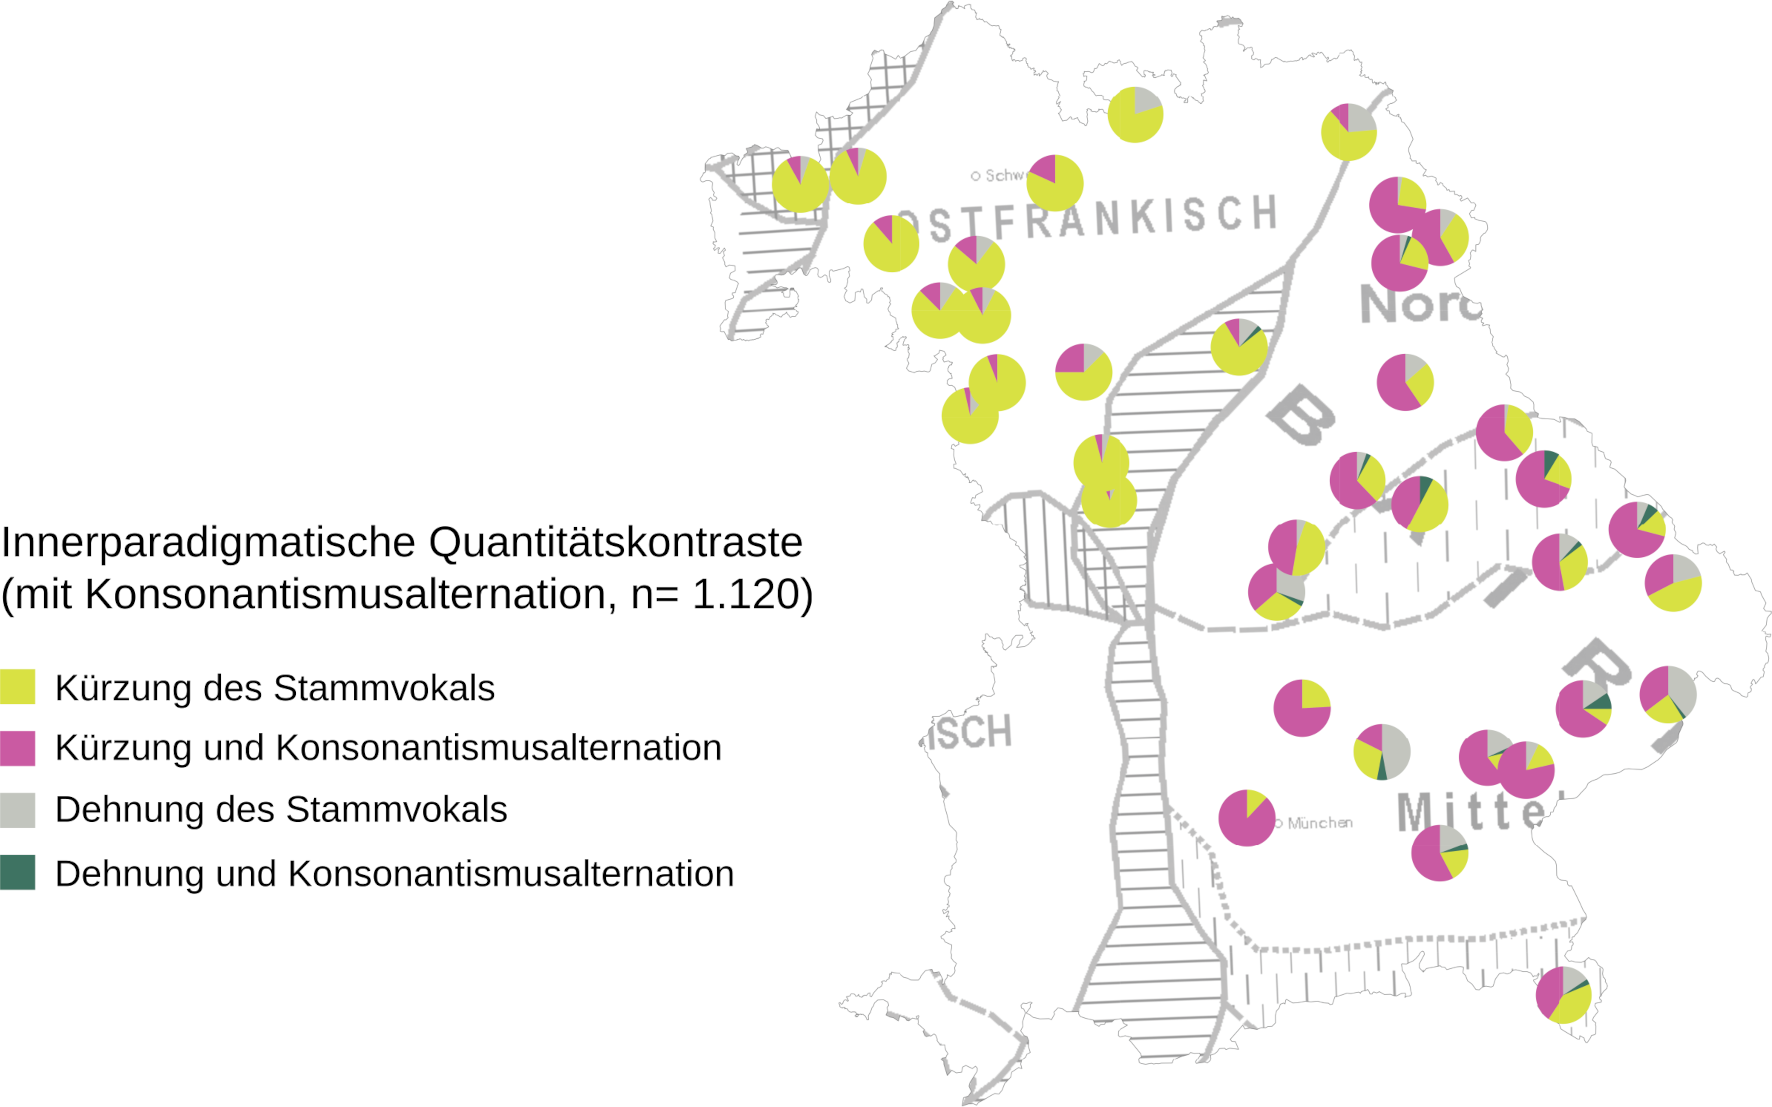
\includegraphics[width=\textwidth]{figures/Karte7.png}
\caption{Häufigkeitsverteilung verschiedener Realisierungen innerparadigmatischer Kontraste der Vokalquantität}
\label{map:7}
\end{map}
\vfill\pagebreak

\mapref{map:8} visualisiert die Häufigkeitsverteilung für Vokalquantitätswechsel des L-K-Musters (d.\,h. Kürzung) für die verschiedenen phonologischen Umgebungen im Auslaut von historischen Einsilbern mit altem Kurzvokal. Quan\-ti\-tät\-kon\-tras\-te bei Lexemen mit altem Kurzvokal vor Obstruent oder Affrikate sind zumeist großräumig belegt.\footnote{Dialektraumspezifisch sind nur die Quan\-ti\-tät\-kon\-tras\-te bei \textit{Brett} im Ofr. und \textit{Griff} im Nord- und Mittelbair., daneben sind sie im gesamten UG, allerdings nur vereinzelt bei \textit{Bett}, \textit{Bloch}, \textit{Fleck}, \textit{Joch}, \textit{Schaff}, \textit{Stadt} und \textit{Weg} belegt.} Vor bestimmten phonologischen Umgebungen, insbesondere bei altem Kurzvokal vor den Konsonantenfolgen /l/ und Konsonant sowie Nasal+Obstruent, sind Quantitätskontraste teilweise regelmäßig ausgeblieben.\footnote{Quantitätskontraste vor /l/ und Konsonant sind nur im nördlichen Nordbair. sowie im westlichen Ofr. zu finden, Einsilberdehnung vor Nasal+Obstruent ist teilweise im Ofr. sowie im nordbair. Tirschenreuth und im mittelbair. Kirchensur nicht belegt. Außerdem sind in den ofr. Tiefenbohrungspunkten Stadtschwarzach und Krum keine Quantitätskontraste in der Abfolge aus altem Kurzvokal und Affrikate belegt.}

Zu den Pluralformen historischer Einsilber zählen neben rein stammaffizierenden Markierungen (Typ fīš -- fiš ‚Fisch‘, frōš -- freš ‚Frosch‘) auch kombinierte Verfahren aus additiver Markierung und Modulation (Quantität, zum Teil in Kombination mit Alternationen der Vokalqualität). Bei zweisilbigen Pluralformen mit geschlossener Silbe sind die innerparadigmatischen Quantitätskontraste lautgesetzlich entstanden. Bei zweisilbigen Pluralformen mit offener Silbe hingegen ist im UG lautgesetzlich Dehnung in offener Tonsilbe eingetreten, allerdings finden sich auch hier im Ofr. und vereinzelt im Bair. innerparadigmatische Quantitätskontraste des L-K-Musters bei \textit{Grab} und \textit{Rad}, bei denen von morphologischen Quantitätskontrasten ausgegangen werden kann: \teuthoo{gro.2}{ɡrōͅ} -- \teuthoo{gre4?wA}{ɡrẹ̈wα} -- Dim. \teuthoo{gre24wAl}{ɡrẹ̄wαl} ‚Grab‘ (nordbair.-mittelbair. Blaibach), \teuthoo{ro2d}{rōd} -- \teuthoo{re):dEy}{re\klammeruntenpost{}{\doubleogonek}də⅄} -- Dim. \teuthoo{ra942dlA}{ra\klammeruntenpost{}̣̄dlα} ‚Rad‘ (ofr. Krum, vgl. \citealt[165]{Rowley1997} und \citealt[Karte 23]{SMF7}). Bemerkenswert ist dabei, dass die Quantitätskontraste hier zum Teil in Ortsdialekten belegt sind (nämlich im ofr. Wilhermsdorf und ofr. Ahorn), die im interdialektalen Vergleich in absoluten Zahlen nur wenige Formen mit Quantitätskontrasten aufweisen, wo diese Form der Pluralmarkierung also ein wenig frequentes Verfahren darstellt (\citealt[110]{SMF7}).


\begin{map}
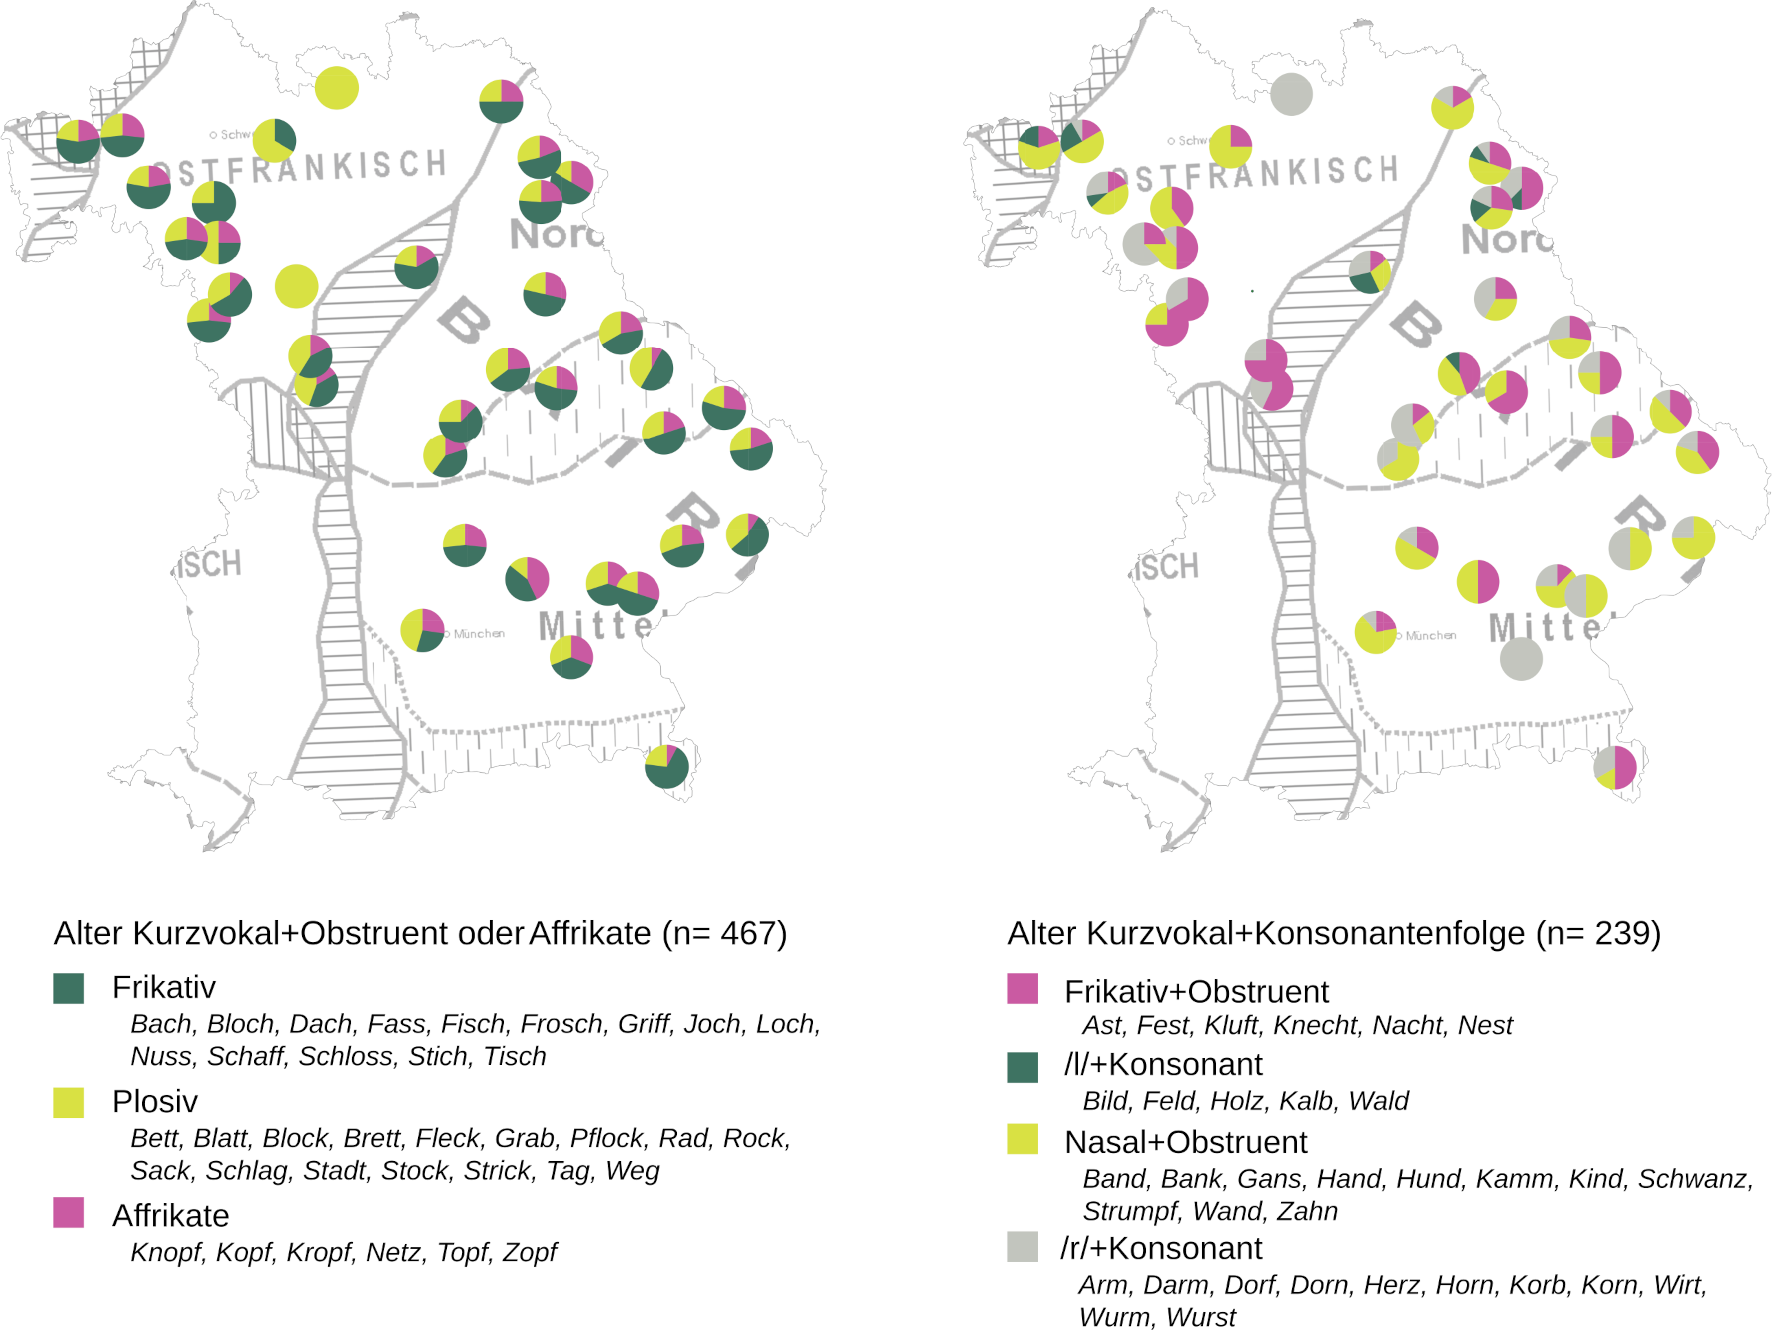
\includegraphics[width=\textwidth]{figures/Karte8.png}
\caption{L-K-Quantitätswechsel bei historischen Einsilbern mit altem Kurzvokal ($n=706$)\protect\footnote{In den BSA-Erhebungen wurde alter Kurzvokal vor Nasal in historischen Einsilbern nur in \textit{Sohn} (keine Belege für innerparadigmatische Quantitätskontraste) und \textit{Mann} (Kürzung in den ofr. und nordbair. Tiefenbohrungspunkten) abgefragt, weshalb diese Umgebung in der Kombinationskarte nicht berücksichtigt wurde. Ebenso nicht berücksichtigt wurde alter Kurzvokal+/l/, das nur in \textit{Stall} abgefragt wurde und im Ofr. sowie vereinzelt im Bair. belegt ist.}}
\label{map:8}
\end{map}

Neben Quantitätskontrasten in historischen Einsilbern mit altem Kurzvokal sind Quantitätskontraste auch bei historischen Einsilbern mit altem Langvokal oder Diphthong belegt (\mapref{map:9}). Während es Ortsdialekte gibt, die Quantitätskontraste bei altem Kurzvokal, nicht aber bei altem Langvokal oder Diphthong aufweisen (ofr. Mitteleschenbach und Hallerstein, bair. Inning am Holz), sind letztere in den Ortsdialekten im westlichen Ofr., im nördlichen Nordbair. sowie vereinzelt im Mittelbair. häufiger belegt. Die Durchsicht der Belege für die einzelnen Ortspunkte zeigt, dass innerparadigmatische Quantitätskontraste bei mhd. Langvokal oder Diphthong in der Tendenz nur vor jenen wortfinalen Konsonanten bzw. Konsonantenfolgen erscheinen, für die sie auch für alte Kurzvokale (d.\,h. als Ergebnis regulärer Einsilberdehnung) zu finden sind.\footnote{Nur in den mittelbair. Ortsdialekten Waldhof und Neukirchen am Inn ist bei \textit{Faust} ein Quantitätskontrast in der Umgebung vor Frikativ+Obstruent belegt, der für alte Kurzvokale nicht belegt ist.} Die phonologische Umgebung des auslautenden Konsonanten bzw. der Konsonantenfolge ist allerdings nur ein Faktor, um diese analogen Quantitätskontraste zu erklären. Insgesamt handelt es sich auch hier primär um lexemspezifische Entwicklungen mit z.\,T. großräumiger arealer Verteilung, so finden sich \textit{Faust}, \textit{Fuß}, \textit{Geiß}{ }und \textit{Haut} im Ofr. und Bair., \textit{Bauch} in den bair. Ortsdialekten, \textit{Schweif} im Mittelbair. und \textit{Stuhl} nur im Ofr.\footnote{In der Teilkarte zur arealen Verteilung wurden jene Lexeme nicht kartiert, die als einzige Vertreter eines mhd. Protovokals belegt sind: \textit{Vieh} (mhd. \textit{ie),} das mit Quantitätskontrast nur im ofr. Gebsattel belegt ist, \textit{Kloß} (mhd. \textit{ô}/\textit{o}, nur in SMF und SUF abgefragt) sowie \textit{Baum} (mhd. \textit{ou}), das im Unterofr. und vereinzelt im Nord- und Mittelbair. Quantitätskontraste aufweist.}


\begin{map}
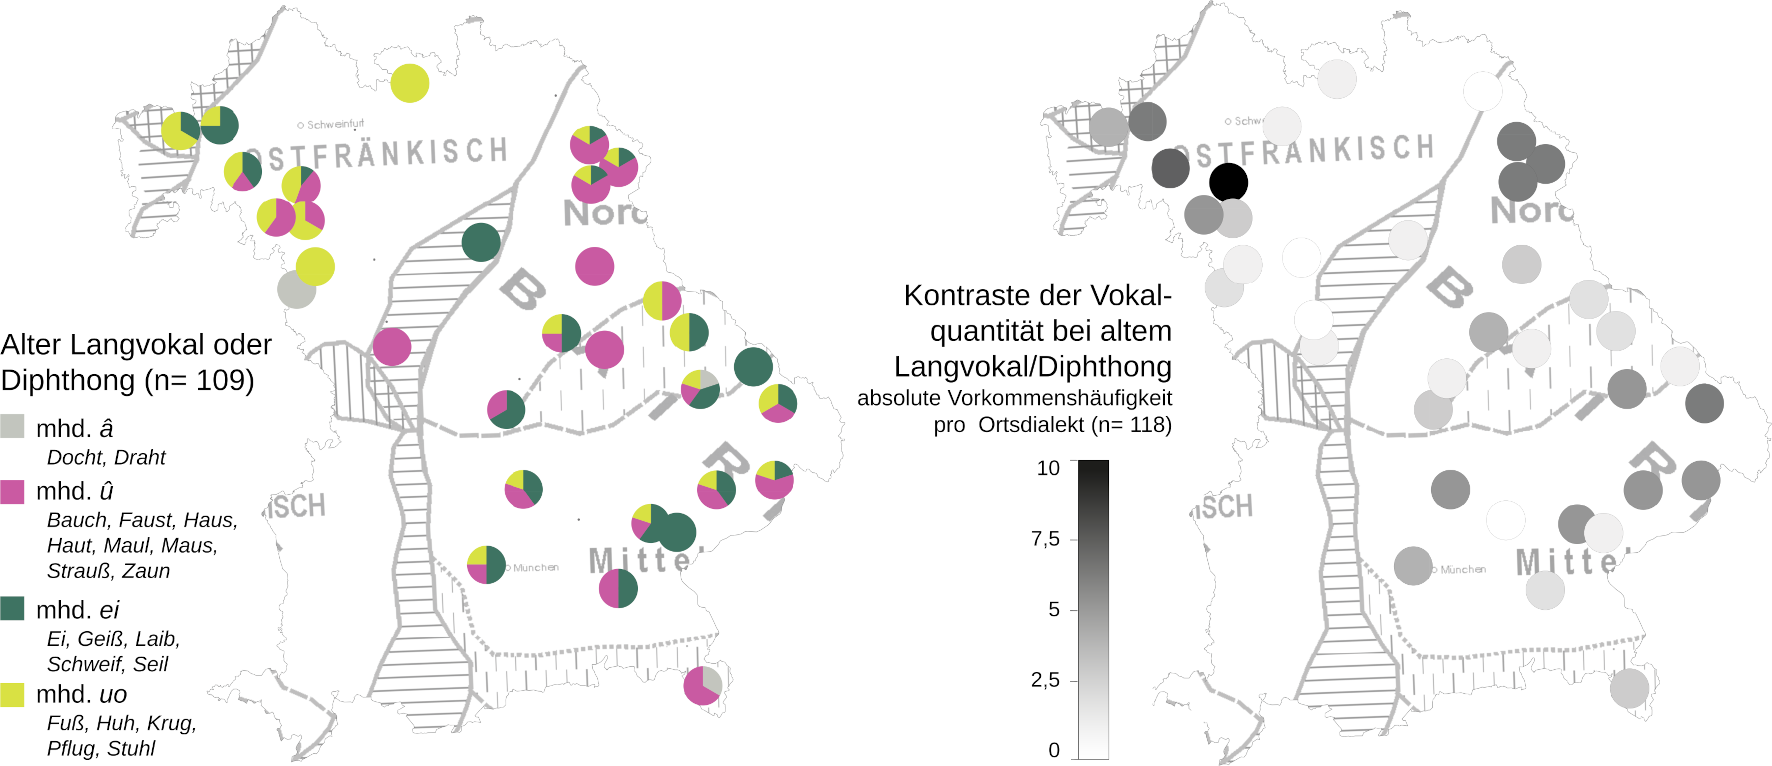
\includegraphics[width=\textwidth]{figures/Karte9.png}
\caption{Häufigkeitsverteilung und absolute Vorkommenshäufigkeit von L-K-Quantitätskontrasten bei altem Langvokal oder Diphthong in historischen Einsilbern}
\label{map:9}
\end{map}

Inwiefern stellen innerparadigmatische Quantitätskontraste nun ein produktives Pluralmarkierungsverfahren dar? Bei historischen Einsilbern mit altem Kurz- und Langvokal können mit Blick auf die BSA-Daten Quantitätsalternationen zwischen lexemspezifischen Lexikalisierungen und genereller Produktivität in Abhängigkeit von der Auslautkonsonanz verortet werden. Wie schwierig die Frage nach der Morphologisierung der Alternationen ist, ist daneben auch an innerparadigmatischen Quantitätskontrasten bei historischen Zwei- und Dreisilbern zu sehen. Die Belege innerparadigmatischer Quantitätsalternation bei historischen Mehrsilbern sind ausgesprochen heterogen, es handelt sich zumeist um vereinzelte Belege, die keine Arealbildung erkennen lassen. Schaut man wiederum auf die absolute Vorkommenshäufigkeit pro Ortsdialekt, so gibt es -- wie auch bei den analogen Quantitätskontrasten bei altem Langvokal oder Diphthong -- Ortspunkte, in denen morphologische Quantitätsalternationen bei historischen Mehrsilbern häufiger vorkommen (mit einem Schwerpunkt in einigen bair. Tiefenbohrungspunkten). In anderen Ortspunkten des UGs, die zwar Quantitätskontraste bei historischen Einsilbern kennen, sind sie für historische Mehrsilber nicht belegt, d.\,h. sie scheinen hier als Pluralmarkierungsverfahren nicht zur Verfügung zu stehen.


\begin{map}
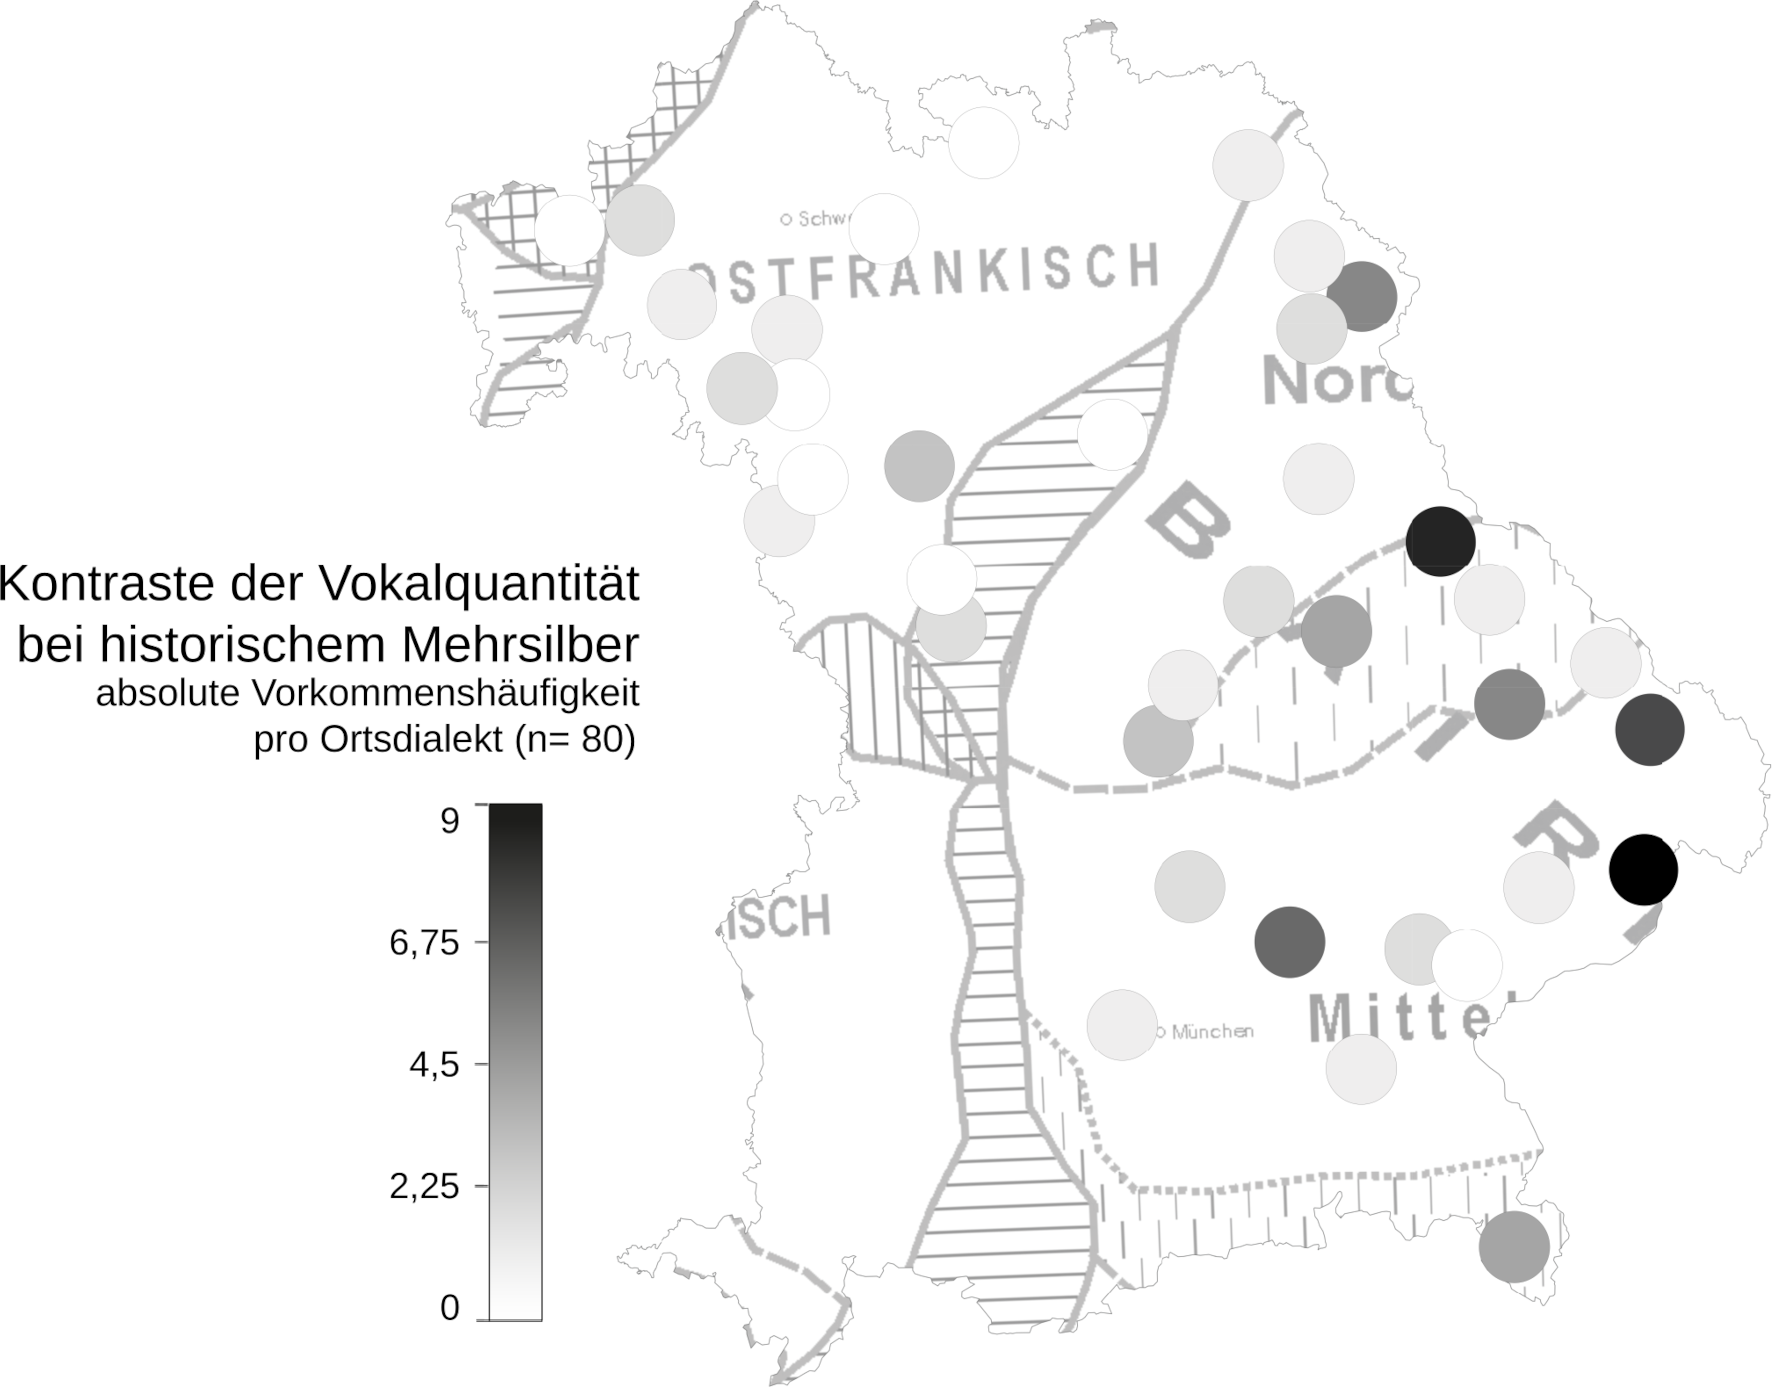
\includegraphics[width=\textwidth]{figures/Karte10.png}
\caption{Chloroplethkarte mit absoluter Vorkommenshäufigkeit von Quantitätskontrasten bei historischen Mehrsilbern}
\label{map:10}
\end{map}

\citegen{Kranzmayer1935} Darstellung zur Entwicklung historischer Zwei- und Dreisilber in oobd. Dialekten eröffnet eine diachrone Perspektive, die zumindest in Teilen eine Erklärung von Quantitätskontrasten bei historischen Mehrsilbern bietet. Lautgesetzlich entstehen im Frühmittelhochdeutschen innerparadigmatische Alternationen zwischen Langvokal in zwei\-silbigen Nominativ-Singular-Formen und Kurzvokal in dreisilbigen Nominativ-Plural-, Dativ-Singular- oder Diminutivformen, z.\,B. Nom.Sg. \teuthoo{va2tEr}{vātər} -- Dat.Sg. \teuthoo{vatEre}{vatəre} im Zimbrischen (vgl. das Vokalquantitätsmuster (c) in \tabref{tab:23}). Nach \citet[82]{Kranzmayer1935} war diese Entwicklung historisch „gemeinoberdeutsch“ und ist im Oobd. zumindest in Restformen bewahrt, darunter in der Region um Ries und Altmühltal sowie in einem oberfränkischen Gebiet um Ebermannstadt und Kulmbach (vgl. die Karte in \citealt[67]{Kranzmayer1935}). \citet[73]{Rowley1997} zufolge ist der lautgesetzliche Zustand in dessen nordostbayrischem UG nicht erhalten, in den vorliegenden Daten finden sich aber durchaus Belege für innerparadigmatische Alternationen bei his\-to\-ri\-schen Zwei- und Dreisilbern (\tabref{tab:24}).\largerpage[-1]

Inwiefern diese Belege tatsächlich einen konservierten lautgesetzlichen Zustand abbilden, muss offenbleiben. Die phonotaktische Umgebung der Erstsilbenkürze, die Dreisilbigkeit, verschwand durch die Apokope bereits im Mittelhochdeutschen in vielen Lexemen, die innerparadigmatische Alternation war damit nicht mehr transparent \citep[83]{Kranzmayer1935}. Gleichzeitig dokumentieren die Beispiele der \tabref{tab:24}, dass (vor der Folie des mhd. Protosystems) sowohl Lexeme mit additiver als auch stammaffizierender Pluralbildung mit innerparadigmatischen Quantitätskontrasten (teilweise in Kombination mit Lenis-Fortis-Kontrasten) belegt sind. Bei historisch starken Substantiven mit Umlautplural und bei historischen Zweisilbern ohne Änderung der Silbenanzahl in der flektierten Form liegen keine lautgesetzlich entstandene Quantitätsalternation vor.

Kranzmayers diachrone Modellierung der Vokalquantität in Abhängigkeit von der historischen Silbenanzahl kann indes einzelne Fälle synchroner Alternationen als konservierte Formen erklären. So deuten die Mehrfachbelege bei \textit{Gabel} darauf hin, dass die von Kranzmayer beschriebenen Verhältnisse im Oobd. großräumige Geltung hatten. Gleichzeitig können diese Formen ein Indiz für eine -- womöglich frühe -- Morphologisierung von Quantitätskontrasten bei zweisilbigen (neben einsilbigen) Stämmen in einzelnen Dialekten sein. Im Folgenden wird bei der Klassifikation von Quantitätskontrasten bei historischen Mehrsilbern konsequent eine synchrone Perspektive eingenommen und von einem morphologisierten Verfahren und analogischen Bildungen ausgegangen.


\begin{table}[p]
\caption{Innerparadigmatische Quantitätskontraste in historischen Zwei- und Dreisilbern im UG (Auswahl, $n=84$)\label{tab:24}}
\begin{subtable}{\textwidth}
\caption{historische Dreisilber\label{tab:24a}}
\small
\begin{tabularx}{\textwidth}{lllQ}
\lsptoprule
mhd. Flexion & {Singular} & {Plural}  & \\\midrule
 stswf. & \teuthoo{ga<vl}{ɡâvl} & \teuthoo{ga94vln}{ɡa\klammeruntenpost{}̣vln} &   ‚Gabel‘ (ofr. Gebsattel, daneben ofr. Pfofeld, mittelbair. Neukirchen am Inn, nordbair. Riedenburg, nordbair.-mittelbair. Grafenkirchen)\\
 \tablevspace
  & \teuthoo{v5e4<dA4}{v̩ệdα̣} & \teuthoo{ve4dAn}{vẹdαn} &   ‚Feder‘ (mittelbair. Inning am Holz)\\
  \tablevspace
 swstf. & \teuthoo{k,\_e2n}{k͓ʰēn} & \teuthoo{k,\_enAn}{k͓ʰenαn} &   ‚Kette‘ (nordbair.-mittelbair. Bernhardswald)\\
 \tablevspace
 stf. & \teuthoo{me.2d}{mēͅd} & \teuthoo{me.xd}{meͅxd} &   ‚Magd‘ (ofr. Stadtschwarzach, daneben ofr. Wilhermsdorf)\\
 \tablevspace
  & \teuthoo{gJo<A4s}{ɡ{\lkreis}ôα̣s} & \teuthoo{gJoA4s\%}{ɡ{\lkreis}oα̣s͈} &   ‚Geleise‘ (südbair.-mittelbair. Ramsau)\\
  \lspbottomrule
\end{tabularx}
\end{subtable}

\begin{subtable}{\textwidth}
\caption{historische Zweisilber mit altem Kurzvokal in offener Silbe\protect\footnote{Daneben belegt sind innerparadigmatische Quantitätskontraste bei \textit{Ader}, \textit{Auge}, \textit{Boden}, \textit{Faden}, \textit{Föhre}, \textit{Haken}, \textit{Hase}, \textit{Hemd}, \textit{Knoten}, \textit{Kröte}, \textit{Magen}, \textit{Name}, \textit{Nagel}, \textit{Säge}, \textit{Säule}, \textit{Schere}, \textit{Schnabel}, \textit{Speiche}, \textit{Stadel}, \textit{Stube}, \textit{Wade}, \textit{Wagen}.}}
\label{tab:24b}
\small
\begin{tabularx}{\textwidth}{llllQ}
\lsptoprule
\makecell[tl]{{mhd.}\\{Flexion}} & {Singular} & {Plural} & \makecell[tl]{Dimi-\\nutiv} & \\\midrule
 swm. & \teuthoo{gro42m}{ɡrọ̄m} & \teuthoo{gra4§(+m}{ɡrạ̃̆\klammerobenpost{}m} &  & ‚Graben‘ (mittelbair. Grafenau)\\
 \tablevspace
  & \teuthoo{bu2}{bū} & \teuthoo{bum}{bum} & \teuthoo{bi“bla}{bībla} & ‚Bube‘ (ofr. Hallerstein, daneben nordbair.-mittelbair. Bernried und Zwiesel)\\
  \tablevspace
 stm. & \teuthoo{he42vA}{hẹ̄vα} & \teuthoo{the4vA}{thẹvα} & \teuthoo{he42vErl}{hẹ̄vərl} & ‚Hafen‘ (nordbair.-mittelbair. Grafenkirchen)\\
 \tablevspace
  & \teuthoo{mae\$bru9.2dE}{mae̤bru\klammeruntenpost{}̄ͅdə} & \teuthoo{mae\$br{\textasciitilde}îidE}{mae̤br{\aufstrih}idə} &  & ‚Bruder‘ (ofr. Wilhermsdorf)\\
  \tablevspace
  & \teuthoo{vo.<ucl}{vôͅuXl} & \teuthoo{vo?.u?cl}{vöͅüXl} & \teuthoo{v5o?.u?cEli}{v̩öͅüXəli} & ‚Vogel‘ (ofr. Stadtschwarzach, daneben nordbair.-mittelbair. Bernhardswald)\\
  \tablevspace
 swf. & \teuthoo{Ata.2om}{αtāͅom} & \teuthoo{ta.om}{taͅom} &  & ‚Taube‘ (nordbair.-mittelbair. Grafenkirchen, daneben mittelbair. Waldhof)\\
 \tablevspace
 swstf. & \teuthoo{no2l}{nōl} & \teuthoo{noln}{noln} &  & ‚Nadel‘ (mittelbair. Grafenau, daneben mittelbair. Inning am Holz)\\
 \lspbottomrule
\end{tabularx}
\end{subtable}
\end{table}


\begin{table}
\ContinuedFloat
\caption{Innerparadigmatische Quantitätskontraste in historischen Zwei- und Dreisilbern im UG (Auswahl, $n=84$)}
\begin{subtable}{\textwidth}
\caption{historische Zweisilber mit altem Kurzvokal in geschlossener Silbe\protect\footnote{Daneben bei \textit{Birne}, \textit{Borste}, \textit{Furche}, \textit{Henne}, \textit{Karren}, \textit{Katze}, \textit{Lärche}, \textit{Ratte}, \textit{Rippe}, \textit{Tochter}, \textit{Wanne}, \textit{Wespe}.}}
\label{tab:24c}
\small
\begin{tabularx}{\textwidth}{lQQl>{\raggedright\arraybackslash}p{.4\textwidth}}
\lsptoprule
\makecell[tl]{mhd.\\Flexion} & {Singular} & {Plural} & {Diminutiv} & \\\midrule
  swm. & \teuthoo{s\#li.“4n}{šlị̄ͅn} & \teuthoo{s\#lin}{šlin} &  & ‚Schlitten‘ (mittelbair. Neukirchen am Inn)\\
  \tablevspace
  & \teuthoo{gðo<At}{ɡ̩ôαt}-\teuthoo{n@}{n̥} & \teuthoo{gða)\$t}{ɡ̩a\klammeruntenpost{}̤t}-\teuthoo{n@}{n̥} & \teuthoo{ga4rtl}{ɡạrtl} & ‚Garten‘ (mittelbair. Grafenau, daneben nordbair. Tirschenreuth)\\
  \tablevspace
 stm. & \teuthoo{ho:"(+mEr}{hō{\doubleogonek}̃\klammerobenpost{}mər} & \teuthoo{ha94mr}{ha\klammeruntenpost{}̣mr} &  & ‚Hammer‘ (ofr. Stadtschwarzach)\\
 \tablevspace
 stf. & \teuthoo{b\_mu.<AtA}{bʰmûͅαtα} & \teuthoo{mu.AtAn}{muͅαtαn} &  & ‚Garten‘ (mittelbair. Niedertaufkirchen, daneben nordbair.-mittelbair. Grafenkirchen, mittelbair. Inning am Holz)\\
 \tablevspace
 stswf. & \teuthoo{se42NSd}{sẹ̄ŋʃd} & \teuthoo{dse4NSdn@}{dsẹŋʃdn̥} &  & ‚Sense‘ (nordbair. Kallmünz, daneben nordbair.-mittelbair. Grafenkirchen, mittelbair. Neukirchen am Inn)\\
 \tablevspace
  & \teuthoo{wu.(<Ed5s5ý@}{wûͅ\klammerobenpost{}əd̩s̩ɫ̥} & \teuthoo{wi.Et,S,ý@}{wiͅət͓ʃ͓ɫ̥} &  & ‚Wurzel‘ (nordbair. Groschlattengrün, daneben nordbair. Oberdolling)\\
  \tablevspace
 swf. & \teuthoo{mu<g-N@}{mûɡ{}͐ŋ̥} & \teuthoo{muk-N@}{muk{}͐ŋ̥} &  & ‚Mücke‘ (mittelbair. Grafenau)\\
\lspbottomrule
\end{tabularx}
\end{subtable}
\end{table}


\subsubsection{Konsonantismuskontraste}\label{sec:7.1.2.3}\largerpage[-1]
Neben Alternationen im Paradigma, die durch Kontraste der Vokalqualität oder -quantität entstehen, affizieren andere Alternationsmuster den Konsonantismus des Stammes. Konsonantismuskontraste finden sich im Auslaut des Stammes und damit an einer Stelle, die -- anders als der Stammvokal -- „für morphologische Symbolisierung nicht primär vorgesehen“ ist \citep[284]{Harnisch1994a}. Phänomene des Konsonantismus werden im Folgenden konsequent aus der -- zugegebenermaßen engen, aber für die Forschungsfrage relevanten -- Perspektive der Flexionsmorphologie behandelt. Der Anspruch ist daher nicht, historische Entwicklungen des Konsonantismus vollständig darzustellen, sondern Ziel ist es, phonetisch-phonologische Entwicklungen aufzuzeigen und zu diskutieren, inwiefern diese für die Kodierung der flexivischen Information funktionalisiert sind. Die Kernfrage des Kapitels lautet folglich: Wann ist lautliche Variation im Konsonantismus zwischen Singular- und Pluralform auf der pho\-ne\-tisch-pho\-no\-lo\-gisch\-en Ebene anzusiedeln, weil sie beispielsweise durch die phonotaktische Position eines Konsonanten in der Wortform bedingt ist? Und wann entsprechen mal isolierte, mal großräumigere Fälle von innerparadigmatischen Konsonantismusalternationen einem Pluralmarkierungsverfahren und damit diachron einer morphologischen Funktionalisierung?


\begin{figure}
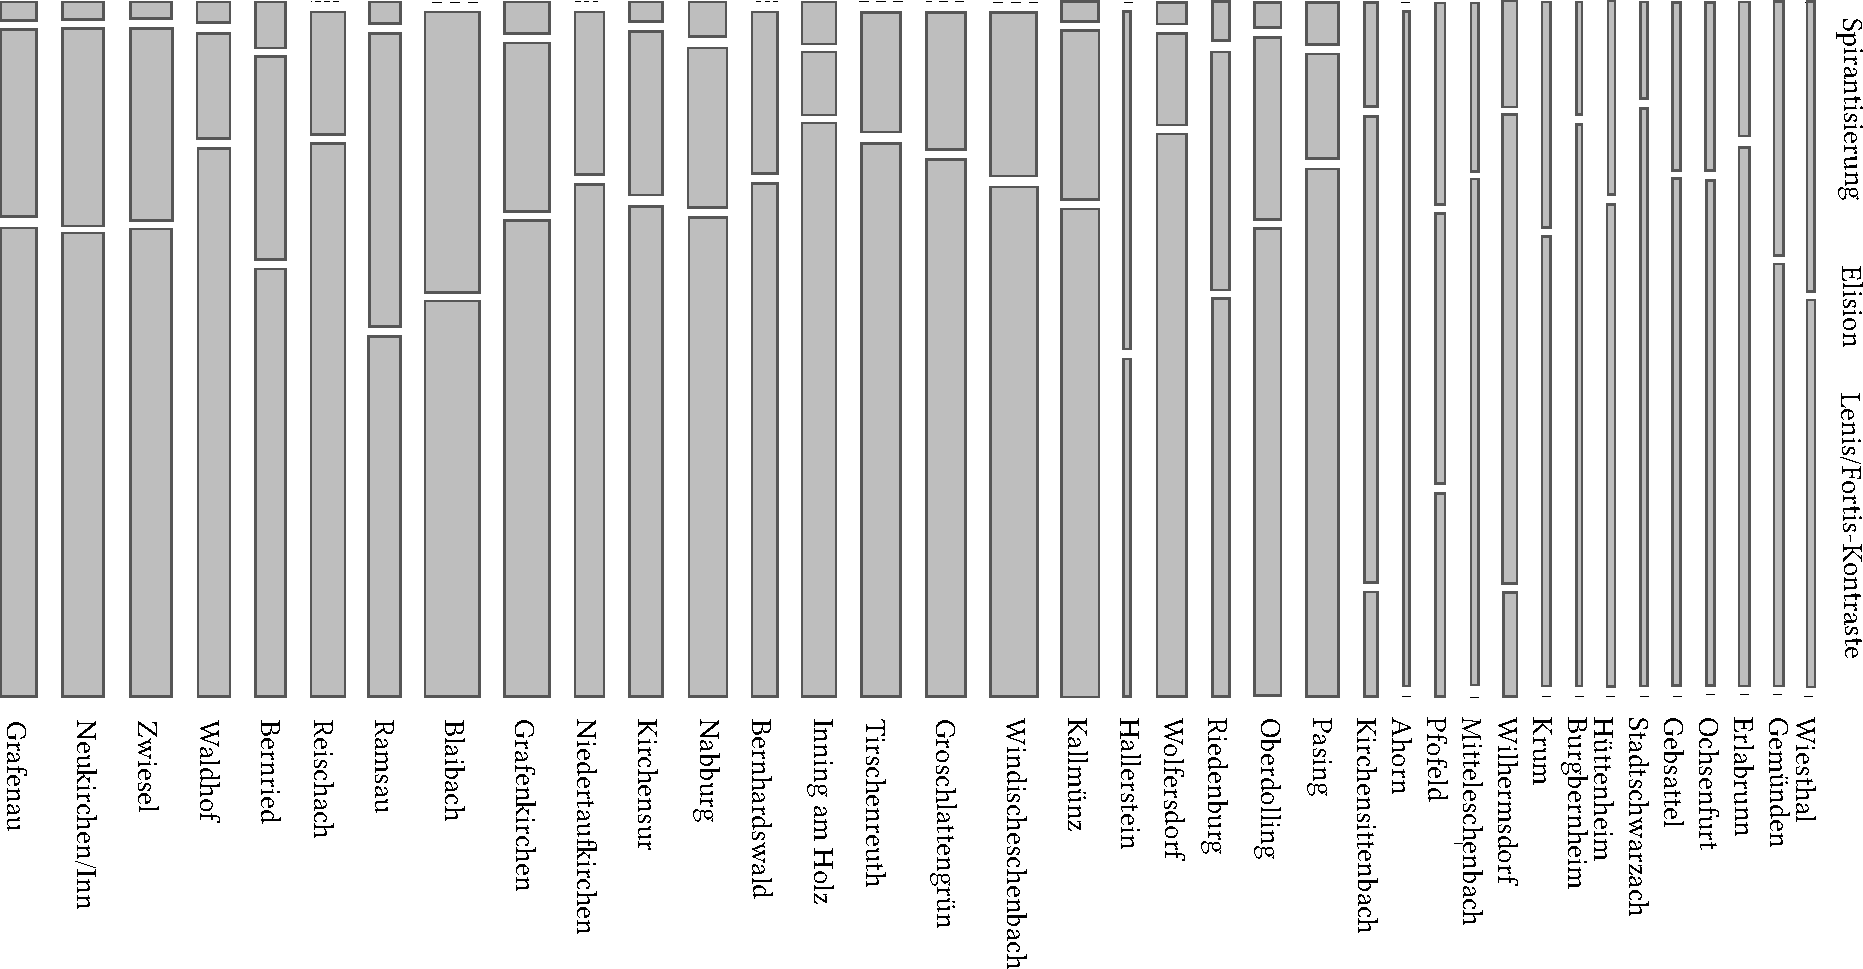
\includegraphics[height=.75\textwidth,angle=90]{figures/revisedNickelNominalmorphologie-img018.pdf}
\caption{Mosaik-Plot mit Häufigkeitsverteilung innerparadigmatischer Konsonantismuskontraste ($n=875$)}
\label{fig:5}
\end{figure}

Innerparadigmatische Konsonantismusalternationen sind -- wie auch die anderen bisher vorgestellten stammaffizierenden Verfahren -- das Ergebnis phonologischer Prozesse. Diese Prozesse sind im Bereich des Konsonantismus in den ofr. und bair. Dialekten unterschiedlich verlaufen (exemplarisch sind hier die sogenannte binnenhochdeutsche und die mittelbair. Konsonantenschwächung zu nennen), woraus auch synchron eine Zweiteilung des UGs resultiert -- sowohl bezogen auf das phonologische als auch auf das zur Verfügung stehende flexionsmorphologische Inventar. Dass es hinsichtlich der verschiedenen Typen von innerparadigmatischen Konsonantismuskontrasten und ihrer relativen Häufigkeit dialektspezifische Unterschiede gibt, illustriert \figref{fig:5}. Das Mosaik-Plot visualisiert die Variablen Ortsdialekt (von West nach Ost), Typus der Konsonantismusalternation und absolute Häufigkeit. Anhand der Größe der Flächen der Rechtecke ergibt sich, dass innerparadigmatische Konsonantismusalternationen in den nord- und mittelbair. Tiefenbohrungspunkten weitaus häufiger belegt sind als in den ofr. Daneben zeigt die Verteilung der verschiedenen Typen, dass es eine dialektspezifische Markierungsstrategie gibt: Lenis-Fortis-Kontraste finden sich nur im Bair. (\sectref{sec:7.1.2.3.1}). Und auch bei innerparadigmatischen Alternationen zwischen elidiertem und erhaltenem Konsonanten gibt es im Bair. spezifische Flexionsmuster, wie in \sectref{sec:7.1.2.3.2} gezeigt wird.

Wie schwierig die Grenzziehung zwischen synchron aktivem phonetisch"=phonologischem Prozess und der Morphologisierung von Konsonantismusalternationen ist, ist exemplarisch an der vokalischen vs. konsonantischen Realisierung von Liquiden zu sehen (\tabref{tab:25}). Im Datenmaterial gibt es Singular- und Pluralformen, bei denen sich durch die additive Markierung der Pluralform innerparadigmatische Alternationen im Stammauslaut zwischen vokalisch realisiertem Liquid im Singular und in intervokalischer Position konsonantisch realisiertem Liquid im Plural ergeben. Die Belege stammen aus dem bair. Teil des UGs, d.\,h. dem Gebiet /l/-Vokalisierung und der konsequenten /r/-Vokalisierung (d.\,h. systematische Vokalisierung von /r/ im absoluten Auslaut wie in \textit{Jahr} und im Auslaut vor Konsonant, z.\,B. \textit{Berg}, \textit{Turm}).\footnote{Die Erhebungen im Rahmen des \textit{Bayerischen Sprachatlas} haben ergeben, dass sich das von \citet{Kranzmayer1956} beschriebene Gebiet der konsequenten \textit{r}{}-Vokalisierung „deutlich nach Westen, teilweise bis an den Lech“ verschoben hat (\citealt[65]{RennKönig2006}). Für das Lexem \textit{Tor} (Typ \teuthoo{do.}{doͅ} -- \teuthoo{dorA}{dorα} oder \teuthoo{deArA}{deαrα}) finden sich daneben auch Belege im Ofr. (vgl. \citealt[§34c4, §49c3 und Karte 26]{Kranzmayer1956}, \citealt[82]{Rowley1997} sowie \citealt[60--99]{SMF4} zur \textit{r}{}-Realisierung im Ofr.).}


\begin{table}
\begin{tabular}{llll}
\lsptoprule
 & {Singular} & {Plural} & \\\midrule
{/r/} & \teuthoo{gs\#i4"4A}{ɡšị̣̄α} & \teuthoo{gs\#i4"4ArA}{ɡšị̣̄αrα} & ‚Geschirr‘ (Kirchensittenbach)\\
& \teuthoo{o.2A4}{ōͅα̣} & \teuthoo{o.2A4rA}{ōͅα̣rα} & ‚Ei‘ (Grafenau)\\
& \teuthoo{s\#do.2dl@do2A}{šdōͅdl̥dōα} & \teuthoo{de2ArA}{dēαrα} & ‚Tor‘ (Nabburg)\\
& \teuthoo{diE}{diə} & \teuthoo{diErAn}{diərαn} & ‚Tür‘ (Blaibach)\\
\tablevspace
{/l/} & \teuthoo{s5ma4<i.}{s̩mậiͅ} & \teuthoo{b-ma4<i.lA}{b{}͐mậiͅlα} & ‚Maul‘ (Grafenau)\\
\lspbottomrule
\end{tabular}
\caption{Beispiele für innerparadigmatische Alternation bei Liquid im absoluten Auslaut in der Singular- und in intervokalischer Position in der Pluralform\label{tab:25}}
\end{table}

In diesen Singular- und Pluralformen ist die Realisierung der Liquiden durch die jeweilige Position in der Wortform bedingt und in der Folge vorhersagbar, Vokalisierung und konsonantische Realisierung von /l/ und /r/ können als Allophone klassifiziert werden. Eine ähnliche Lösung bietet sich auch für intervokalische Spirantisierungen an (\sectref{sec:7.1.2.3.3}) und für additive Formen mit erhaltenem Obstruenten (\sectref{sec:7.1.2.3.2}). Formenbildung an der Schnittstelle zwischen Phonologie und Morphologie ist hier stärker in der Phonologie zu verorten und primär durch phonologische Prozesse gesteuert. Gleichzeitig erscheinen die Alternationen sehr regelmäßig in Flexionsformen, sodass sie durchaus als „begleitende“ morphophonologische Marker funktionalisiert sein könnten und als solche perzipiert werden (und entsprechend kognitiv verankert sind).

\subsubsubsection{Lenis-Fortis-Kontraste}
\label{sec:7.1.2.3.1}
\begin{quote}
Die Darstellung der Quantität ist das Einfachste und zugleich das Schwierigste in der bair. mda. [Mundart, GN]. \citep[12]{Kollmer1949}
\end{quote}

Im bair. Teil des UG sind innerparadigmatische Kontraste zwischen Lenis- und Fortisobstruenten durch das sogenannte „bairische Silbengesetz“ (auch Pfalzsche Regel, vgl. \citealt{Pfalz1913, Pfalz1936}) bedingt: Im Auslaut der Haupttonsilbe folgt Leniskonsonanz auf Langvokal, auf Kurzvokal hingegen Fortiskonsonanz (vgl. 	\tabref{tab:26}). Die Opposition zwischen Lenis- und Fortis-Konsonant besteht dabei weniger in einem Kontrast der Konsonantenstärke als vielmehr in einem Kontrast der Konsonantenquantität (vgl. \citealt[33--35]{Bachmann2000}, \citealt[30]{Hinderling1980}, \citealt[177]{Kufner1957}, \citealt[14]{Schießl1909}, \citealt[240]{Seiler2009} sowie \citealt[30]{Auer1991}).


\begin{table}
\begin{tabular}{llll}
\lsptoprule
 Langvokal\,+\,Leniskonsonanz & \multicolumn{2}{l}{Kurzvokal\,+\,Fortiskonsonanz} & \\
 {VːC\textsubscript{lenis}} & \multicolumn{2}{c}{VC\textsubscript{fortis}} & \\\cmidrule(lr){1-1}\cmidrule(lr){2-3}
 Nom.Sg. & Nom.Pl. & Diminutiv & \\  \midrule
 \teuthoo{gri“v}{ɡrīv} & \teuthoo{grI3f}{ɡrı̆f} &  & ‚Griff‘\\
 \teuthoo{hu<nd}{hûnd} & \teuthoo{hu3nt\_}{hŭntʰ} & \teuthoo{hu3ntÿ}{hŭnt\ɫ} & ‚Hund‘\\
 \teuthoo{di“s\#5}{dīš̩} & \teuthoo{dI3S}{dı̆ʃ} &  & ‚Tisch‘\\
\cmidrule(lr){1-2}
\multicolumn{2}{c}{ {Minimalpaare}} &  & \\
\lspbottomrule
\end{tabular}
\caption{Beispiele für innerparadigmatische Lenis-Fortis-Kontraste mit Minimalpaaren aus dem nordbair. Groschlattengrün}
\label{tab:26}
\end{table}

Die Lenis-Fortis-Opposition ist ein Spezifikum des nord- und mittelbair. Teils des UGs, und zwar sowohl aus phonologischer als auch aus flexionsmorphologischer Perspektive. \citet[59]{Seidelmann2013} sieht in dem Kontrast zwischen Lenis und Fortis denn auch „die zentrale Opposition im phonologischen System des Mittelbairischen“ und die sog. mittelbairische und die binnenhochdeutsche Konsonantenschwächung als „zwei konträr organisierte Systeme“ (\citealt[60]{Seidelmann2013}, vgl. \citealt[34--35]{Steger1968}). Infolge der verschiedenen phonologischen Prozesse, die nach \citet[§34]{Kranzmayer1956} zur „mittelbair. Konsonantenschwächung“ gezählt werden (darunter die Lenisierung von Fortes im In- und Auslaut nach Langvokal, vgl. \tabref{tab:33}), sind Vokal- und Konsonantenquantität im Nord- und Mittelbair. korreliert. Im Ofr. hingegen ist die distinktive Opposition zwischen mhd. Lenes und Fortes als Ergebnis der binnenhochdeutschen Konsonantenschwächung in allen Positionen aufgehoben; in Minimalpaaren wie ofr. \teuthoo{vI2s\#}{vı̄š} -- \teuthoo{vis\#}{viš} ‚Fisch‘ ist der Kontrast der Vokalquantität das relevante Merkmal.


\begin{map}
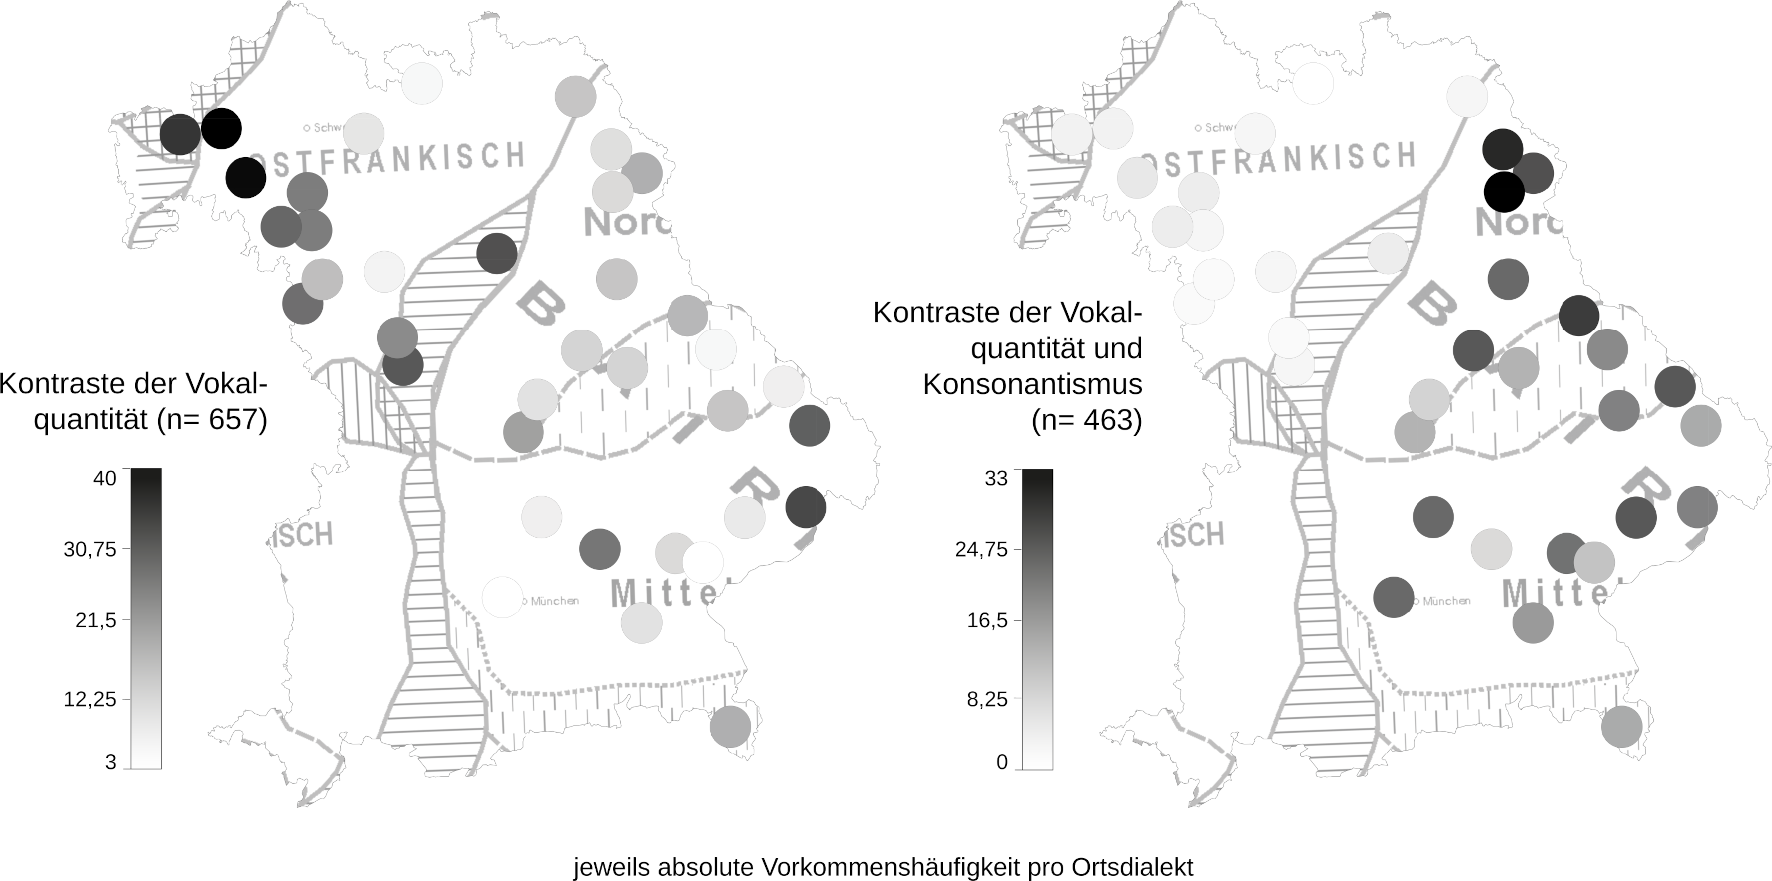
\includegraphics[width=\textwidth]{figures/Karte11.png}
\caption{Chloroplethkarten zur absoluten Vorkommenshäufigkeit von Quantitätskontrasten vs. Quantitäts- und Konsonantismuskontrasten ($n=1.120$)}
\label{map:11}
\end{map}

Synchron spiegelt sich die divergente Entwicklung der phonologischen Systeme im Ofr. und im Nord- und Mittelbair. hinsichtlich Vokalquantität und Konsonantismus in den stammaffizierenden Pluralmarkierungsstrategien wider. Die Chloroplethkarten in \mapref{map:11} illustrieren, dass es für die absoluten Häufigkeiten stammaffizierender Pluralmarkierungen, die die Quantität von Stammvokal sowie von in- und auslautendem Konsonantismus betreffen, in der Tendenz eine Zweiteilung gibt: Während sich Kontraste der Vokalquantität in allen Tiefenbohrungspunkten, schwerpunktmäßig aber in den Ortspunkten des westlichen Ofr. finden, sind Kontraste, die die Vokalquantität in Kombination mit Lenis-Fortis-Kontrasten betreffen, nur in den bair. Ortsdialekten nachweisbar.

Ausgangspunkt aller Analysen zum Phänomen -- diachroner wie synchroner -- sind die rezenten Quantitätsverhältnisse im Nord- und Mittelbair. „Unkontrovers“ ist laut \citet[343]{MoosmüllerScheutz2018}, dass diese aus einer zweimorigen Silbenstruktur resultieren und ein Beispiel von „mora compensation“ \citep[1080]{Auer1989} darstellen, d.\,h. von kompensatorischem Quantitätenausgleich im phonologischen Wort.\footnote{In Einsilbern folgt Morenkompensation auf der Wortebene denselben Prinzipien wie bei Morenkompensation in der Silbe \citep[1082]{Auer1989}.} In der Silbe sind die Quantitäten von Vokal und Konsonant komplementär zueinander verteilt: Auf einen kurzen (einmorigen) Vokal folgt ein Fortiskonsonant (dieser entspricht einer einmorigen Geminate),\footnote{Geminate wird hier und im Folgenden in der Definition von \citet[108]{Seiler2005} verwendet, „i.e., a geminate is a consonant that is underlyingly moraic and phonetically long [\ldots].“ Geminaten in dieser Definition können im Inlaut (ambisilbisch) und wortfinal im Auslaut erscheinen.}  auf einen langen (zweimorigen) Vokal folgt ein nicht-morenwertiger Leniskonsonant bzw. -Konsonantencluster (vgl. \citealt[342]{MoosmüllerScheutz2018}, \cites[113]{Seiler2005}[260]{Seiler2009}).\footnote{In dem Artikel „Some ways to count morae“ zählt \citet[1090]{Auer1989} anders, da das phonologische Wort im Bair. drei Moren umfasse (ebenso \citealt[35]{Hinderling1980}). In einer Wortform wie [re:d] ‚rede (1.Ps.Sg.Präs.)‘ ist der Langvokal danach zweimorig, der Leniskonsonant einmorig (vgl. \citealt[11]{Auer1991}). Auers morentheoretische Analyse unterscheidet sich außerdem dahingehend, dass Geminaten nicht wortfinal erscheinen können und daher regelbasiert reduziert werden (\citealt[1093]{Auer1989}, vgl. \citealt[14]{Auer1991}). Wortformen mit wortfinaler Geminate wie Pl.
\textit{fischsch} ‚Fisch‘ modelliert \citet[1094--1095]{Auer1989} in ihrer lexikalischen Repräsentation mit einer leeren More, die einem Silbenkern entspricht und nicht durch ein Segment besetzt wird.}\largerpage

Kontrovers ist hingegen, welches der beiden korrelierenden Merkmale Träger der Merkmalsopposition und welches phonologisch nicht distinktiv ist. Dialektologische Arbeiten mit (morpho)phonologischem Schwerpunkt (\citealt{Dozauer1967}, \citealt{HarnischRowley1990}, \citealt{Hinderling1980}, \citealt{Kufner1957}, \citealt{Rowley1997}, \citealt{Wiesinger1990}) sehen das relevante Merkmal in der Lenis-Fortis-Opposition, die Vokallänge dagegen ist allophonisch (hierzu kritisch \citealt[355]{MoosmüllerScheutz2018}). \citet{Bannert1976} bietet mit seinen instrumentellen Quantitätsmessungen eine frühe empirische Untersuchung und ein zweites Erklärungsmodell, das nicht die Lenis-Fortis-Opposition, sondern eine prosodische Größe als phonologisch distinktives Merkmal definiert: die komplementäre Relation von Vokal und Konsonant. Vokal und Folgekonsonant werden in dieser Analyse als eine Einheit aufgefasst, deren jeweilige Anteile sich in der Lenis- vs. Fortisrelation komplementär zueinander verhalten; unabhängig von der absoluten Dauer ist die komplementäre Relation konstant groß.\footnote{Die Grundstruktur der komplementären Länge zwischen Vokal und nachfolgendem Konsonanten beträgt im Verhältnis im Lenisfall 3:1, im Fortisfall 2:3 \citep[87]{Bannert1976}. Die Analyse einer komplementären Länge von Vokal und Konsonant findet sich als Konzept des Silbenschnitts bereits bei \citet{Sievers1976}, \citet{Pfalz1913} oder -- aus strukturalistischer Perspektive -- bei \citet{Trubetzkoy1977}.}

Wie die rezenten Quantitätsverhältnisse als Spezifikum des Nord- und Mittelbair. diachron entstanden sind, rekonstruiert \citet{Seiler2005, Seiler2008, Seiler2009} mit einer phonologischen Analyse der Lautwandelprozesse. In Seilers Interpretation stellt auch der Konsonantismus, genauer: dessen Morenwertigkeit, eine Bedingung für Veränderungen der Vokalquantität und folglich das relevante Merkmal dar \citep[267]{Seiler2009}. Die innerparadigmatische Alternation zwischen Lang\-vo\-kal\,+\,Le\-nis und Kurz\-vo\-kal\,+\,For\-tis ist das Ergebnis verschiedener regulärer Lautveränderungen (\cites[187]{Seiler2008}[244--245]{Seiler2009}, vgl. \citealt[§34k2-3]{Kranzmayer1956}):\largerpage

\begin{itemize}
\item \textit{Finale} \textit{Geminatenkürzung}: Im absoluten Auslaut erfolgte Kürzung (auch Lenisierung) von Geminaten (Sg. \teuthoo{tiS'S'}{tiʃ̌ʃ̌} > \teuthoo{tiS'}{tiʃ̌} ‚Tisch‘, vgl. auch \citealt[20--21]{Lessiak1933}). Infolge der Apokope des Schwa der Pluralform (Pl. \teuthoo{tiS'S'E}{tiʃ̌ʃ̌ə} > \teuthoo{tiS'S'}{tiʃ̌ʃ̌}) entsteht die innerparadigmatische Alternation zwischen Lenis im Singular und Fortis (d.\,h. Geminate) im Plural (vgl. \citealt[1098]{Wiesinger1983a}).
\item \textit{Einsilberdehnung}: Vokale in Einsilbern werden gedehnt, wenn ein einzelner Konsonant in der Silbenkoda folgt (dabei spielt es keine Rolle, ob der Einzelkonsonant das Ergebnis von finaler Geminatenkürzung ist, vgl. \citealt[259]{Seiler2009}). Den Erklärungsansatz liefert die Morentheorie im Sinne von \citet{Hayes1989}: Dialekte, die Einsilberdehnung durchgeführt haben, haben eine mindestens zweimorige Silbenstruktur (vgl. \citealt[259]{Seiler2009}). Ist der Konsonant nicht-morenwertig, wird der einmorige Kurzvokal zu einem zweimorigen Langvokal gedehnt.
\item \textit{Reanalyse} \textit{und} \textit{„analogical} \textit{grammar} \textit{simplification“} \citep[122]{Seiler2005}: Da „\textit{most} long vowels“\footnote{Wenngleich diese frequenzbasierte Annahme plausibel scheint, fehlt m.\,E. die Fundierung durch tatsächliche Frequenzwerte. Grundsätzlich fällt in der Diskussion um die bair. Quantitätsverhältnisse auf, dass sich die Forschungsdiskussion in weiten Teilen auf dieselben Beispielbelege in \citet{Pfalz1913, Pfalz1936} und \citet{Kufner1957} bezieht (vgl. die Kritik in \citealt[344]{MoosmüllerScheutz2018} sowie \citealt{Seidelmann2013}).} gedehnte Vokale waren, geht \citet[117]{Seiler2005} davon aus, dass alle Langvokale als gedehnte Vokale generalisiert (d.\,h. reanalysiert) wurden. Infolge der Reanalyse sind Langvokale im Mittelbair. nicht mehr lexikalisch spezifiziert, sondern das Ergebnis einer einzigen Regel: „stressed vowels are short in syllables closed by geminates; otherwise, stressed vowels are long“ \citep[118]{Seiler2005}.
\end{itemize}

Als Ergebnis dieser Prozesse (insbesondere der Reanalyse und Regelvereinfachung) ist Vokalquantität im phonologischen System des Mittelbair. nicht mehr distinkt, sondern nach \citet[122]{Seiler2005} regelbasiert vorhersagbar, wenn eine bimorische Silbenstruktur des Bair. und der Lenis-Fortis-Kontrast als relevantes Merkmal zugrunde gelegt wird. Die spezifische Kombination der Lautwandelprozesse im Mittelbair. stelle dabei eine notwendige, aber keine hinreichende Bedingung für die rezenten Quantitätsverhältnisse dar, wie ein Vergleich der Vokalquantität im Südbair. zeigt (\citealt[121--122]{Seiler2005}, vgl. \citealt[§34k und Karte 22]{Kranzmayer1956}).

Die phonologischen Prozesse, die Seiler in seiner diachronen Rekonstruktion ansetzt (finale Geminatenkürzung, Apokope und Einsilberdehnung), nimmt \citet{Hinderling1980} in ähnlicher Form für seine synchrone phonologische Interpretation der innerparadigmatischen Lenis-Fortis-Alternationen an.\footnote{Seine Analyse ist insofern „morphophonemisch“, als er „Tatbestände der Morphologie“ in seine generative phonologische Analyse einbezieht \citep[28--29]{Hinderling1980}.} In additiven Flexionsformen wie den Verbformen 1.Ps.Sg. [re:d] vs. 2.Ps.Sg. [retsst], 3.Ps.Sg. [ret] ‚reden‘ folgt der innerparadigmatische Wechsel einem „phonologischen Mechanismus“ \citep[30]{Hinderling1980}: Durch „fortis-lenis-relevante“ Suffixe\footnote{\citet[31]{Hinderling1980} unterteilt Stämme und Suffixe danach, ob sie „fortis-lenis-relevant“ oder „fortis-lenis-neutral“ sind, d. h. entweder einen Lenis- oder Fortisobstruenten enthalten oder auf Vokal, Diphthong oder „nicht oppositionsfähigen“ Nasal auslauten.} wie die Flexive der 2. und 3.Ps.Sg. entsteht tiefenstrukturell eine Konsonantenverbindung, die Formen [retsst], [ret] werden /red+sd/, /red+d/ phonologisiert (ebd.: 32--36). Ausgehend von der Annahme, dass wortfinale Geminaten im Bair. lenisiert (d.\,h. gekürzt) werden, modelliert \citet[39]{Hinderling1980} für die Lenis-Fortis-Alternation bei oberflächenstrukturell endungslosen Pluralformen des Typs [fi:š] -- [fišš] ‚Fisch‘ eine Tiefenstruktur mit Endung im Pl.: /fišš/ -- /fišša/. Der „phonetische ‚Ausstoß‘“ \citep[39]{Hinderling1980} ist das Ergebnis dreier Transformationsregeln: (1) wortfinale Lenisierung des Fortiskonsonanten (d.\,h. Geminantenkürzung), (2) Dehnung des Kurzvokals vor Leniskonsonant, (3) Tilgung des /a/ der Pluralform (\citealt[39]{Hinderling1980}, kritisch hierzu \citealt[17]{Scheutz1984}). Auch historisch apokopierte Singularformen wie mhd. \textit{bette} ‚Bett‘ und mhd. \textit{ratze} ‚Ratte‘ sind in der Analyse \citegen[44]{Hinderling1980} mit einem stummen /a/ phonologisiert (d.\,h. einem „Stammbildungssuffix“, \citealt[76]{Harnisch1995}): [bet]=/bedda/, [rats]=/radda/.

Die beiden vorgestellten phonologischen Analysen -- ebenso wie die morphophonologische Analyse, die \citet{Harnisch1995, Harnisch2016} aus Perspektive der Natürlichen generativen Phonologie vornimmt -- haben gemein, dass sie ausgehend von ihrem jeweiligen regelbasierten Ansatz die rezenten bair. Quantitätsverhältnisse als vorhersagbar, das komplementäre Verhältnis von Vokalquantität und Lenis-Fortis-Konsonanz als „strikt“ \citep[70]{Harnisch1995} modellieren. Singular- und Pluralformen wie \teuthoo{he3Ed5s5\#}{hĕəd̩š̩} -- \teuthoo{he3EtSA}{hĕətʃα} ‚Herz‘ (nordbair. Windischeschenbach) oder \teuthoo{vi“s\#}{vīš} -- \teuthoo{vi“S'}{vīʃ̌} ‚Fisch‘ (mittelbair. Pasing), bei denen auf einen Kurzvokal im Singular eine Lenisaffrikate, respektive auf einen Langvokal im Plural ein Fortiskonsonant folgt, widersprechen diesen Vorhersagen. Wie können diese innerparadigmatischen Alternationen aus flexionsmorphologischer Perspektive nun modelliert, welches Kodierungsverfahren kann angesetzt werden?

Diachron (und synchron) weisen Quantitätskontraste durch die innerparadigmatischen Alternationen in nominalen Flexionsformen „a particular degree of saliency“ \citep[116]{Seiler2005} auf (und gleichzeitig eine hohe Gebrauchsfrequenz), sie sind im Nord- und Mittelbair. als Pluralmarker funktionalisiert (vgl. \cites[118]{Seiler2005}[195]{Seiler2008} sowie \citealt[16]{Pfalz1936}, \citealt[123]{Rowley1997}). Dennoch widerspricht die Realität der Daten der Annahme einer „strikten“ Korrelation. Dass es eine freie Varianz der Vokalquantität im (Mittel-)Bair. gibt, zeigt auch \citet{Seidelmann2013} anhand von Belegen in Ortsgrammatiken und Sprachatlasbänden. Er kommt zu dem Schluss, dass es weniger eine feste Korrelation von Vokal- und Konsonantenquantität als „vielmehr eine maximal freie Sprechrhythmik und sprechstilistische Modellierbarkeit ohne phonologische Relevanz der Vokal- (und Kon\-so\-nan\-ten-)""dauer“ \citep[61]{Seidelmann2013} gibt. Kern der Pfalzschen Regel sei „die maximale Profilierung des Fortis-Lenis-Gegensatzes im Mittelbairischen, mit unterstützender Differenzierung der Vokaldauer, aber sie ist keine Performanzregel und begründet keinen phonetischen Automatismus“ (\citealt[61]{Seidelmann2013}, ähnlich in \citealt{Seidelmann2002}).\footnote{Ähnliches beschreibt \citet{Denz1977} in seiner Ortsgrammatik zu Windischeschenbach. Die Vokalquantität biete eine „Unterscheidungshilfe“, ob Lenis oder Fortis vorliegt, obgleich „der Quantitätengegensatz der Vokale beim Sprechen oft relativ unscharf ist, aber auch die Stärke bzw. Dauer der Konsonanten nicht in allen Wortstellungen und in jeder lautlichen Nachbarschaft gleich deutlich wird.“ \citep[72]{Denz1977}.} Interessant ist in diesem Zusammenhang der Gedanke, dass der Varianz, die Seidelmann in den Daten der Dialektmonografien gefunden hat, „eine Normvorstellung, die genau der von Pfalz formulierten Regel entspricht“, gegenübersteht \citep[60]{Seidelmann2013}. Das bair. Silbengesetz stelle daher eher einen „Rahmen“ dar, „der unterschiedliche Füllungen, ja auch Modifikation zulässt“ \citep[104]{Seidelmann2002}.

Daneben liefern diverse jüngere instrumentalphonetische Studien Evidenz für eine weniger feste Korrelation von Vokal- und Konsonantenquantität. So kommen \citet{MoosmüllerScheutz2018} in ihrer instrumentalphonetischen Studie mit zwei ostmittelbair. Gewährspersonen zu dem Ergebnis, dass Bannerts Modell einer komplementären Relation nur eingeschränkt gilt. Sie finden für Lenes und Fortes variierende Relationswerte und gehen davon aus, dass „bereits ein geringfügiges Übergewicht des Vokals bzw. des Konsonanten ausreicht, um den jeweils entgegengesetzten Eindruck hervorzurufen“ (\citealt[357]{MoosmüllerScheutz2018}). Bereits \citet{Scheutz1984, Scheutz1985} kommt zu dem Fazit, dass es Schwellenwerte sind, die zu einem Lenis- oder Fortiseindruck führen. Quantität stelle zwar einen Faktor bei der Diskrimination von Lenes vs. Fortes dar, aber weder Quantität noch die komplementäre Relation von Vokal und Konsonant noch andere in der Forschung diskutierte Merkmale können „zweifelsfrei als alleiniger, unabhängiger Distinktionsträger eruiert werden“, daher gehe er „bis zum Erweis des Gegenteils entgegen dem phonologischen Usus von einer ‚Mehrfachmarkierung‘ aus“ (\citealt[160]{Scheutz1985}, ähnlich \citealt[27]{Scheutz1984}).\footnote{Ein ähnliches Fazit zieht \citet[17]{Kleber2017}: „[\ldots] differences in consonant duration should not be interpreted as signaling a phonemic fortis-lenis contrast; instead they contribute together with different vowel durations to phonemic complementary length.“}  Die Studien von \citet{KlinglerEtAl2017} und \citet{MoosmüllerBrandstätter2014} zeigen außerdem, dass sich im Mittelbair. Sequenzen aus Langvokal und Fortis (VːC\textsubscript{fortis}) nachweisen lassen, die von Bannerts Modell und \citet{Pfalz1913} nicht berücksichtigt wurden (und beiden jeweils widersprechen), und zwar sowohl in zweisilbigen CVCV-Sequenzen als auch in Einsilbern. \citet{Kleber2017} weist in einem intergenerationellen Vergleich von älteren und jüngeren Mittelbairisch- und Sächsischsprechern zudem nach, dass der Unterschied zwischen Sächsisch- und Bairischsprechern in der älteren Generation größer ist als bei der jüngeren, d.\,h. dass das Dialektmerkmal der komplementären Länge zur jüngeren Generation hin in Produktion wie Perzeption abgebaut wird und dass Vokalquantität bei jüngeren Sprechern tendenziell unabhängig von der Quantität des Konsonanten realisiert wird (während Vokal- und Konsonantenquantität bei den älteren Sprechern korreliert, vgl. \citealt[12 und 18]{Kleber2017}).

\subsubsubsubsection{Lenis-Fortis-Kontraste zwischen Phonetik, Phonologie und Morphologie in den BSA-Daten}

Die Daten des \textit{Bayerischen Sprachatlas} bestätigen die Ergebnisse der instrumentalphonetischen Studien insofern, als die innerparadigmatischen Quantitätsverhältnisse (bezogen auf Vokal- und Konsonantendauer) vielfältiger und komplexer sind, als es der Terminus Bair. Silben\textit{gesetz} impliziert. Die beiden Übersichtskarten in \mapref{map:12} zeigt, dass sich innerparadigmatische Lenis-Fortis-Al\-ter\-na\-tio\-nen in allen bair. Tiefenbohrungspunkten finden, daneben in Form von Einzelbelegen im ofr.-nordbair. Übergangsgebiet sowie im ofr. Hallerstein und Wilhermsdorf. Die innerparadigmatische Alternation kann entweder darin bestehen, dass im Singular Leniskonsonanz, im Plural Fortiskonsonanz (jeweils in Kombination mit oder ohne Kontrast der Vokalquantität) oder im Singular Fortiskonsonanz, im Plural Leniskonsonanz (mit oder ohne Kontrast der Vokalquantität) erscheint. Damit ist die Realität der sogenannten „Wechselparadigmen“ \citep[37]{Hinderling1980} vielfältiger als Lenis im Singular, Fortis im Plural (vgl. \citealt[123]{Rowley1997}). Nach \citet[179]{Scheutz1985} sind Lenis-Fortis-Kontraste in flektierten Wortformen „synchron eben gerade nicht (mehr) transparent und voraussagbar, sondern an morphologische Regularitäten geknüpft oder überhaupt lexikalisiert.“ Die Daten zeigen indes, dass \citeauthor{Scheutz1984}' (\citeyear[17]{Scheutz1984}) Aussage, dass für Singular und Plural „ganz bestimmte Quantitätsverhältnisse verknüpft werden“, einen (wenn auch kleinen) Teil der Alternationen nicht erklärt.

\vfill
\begin{map}[H]
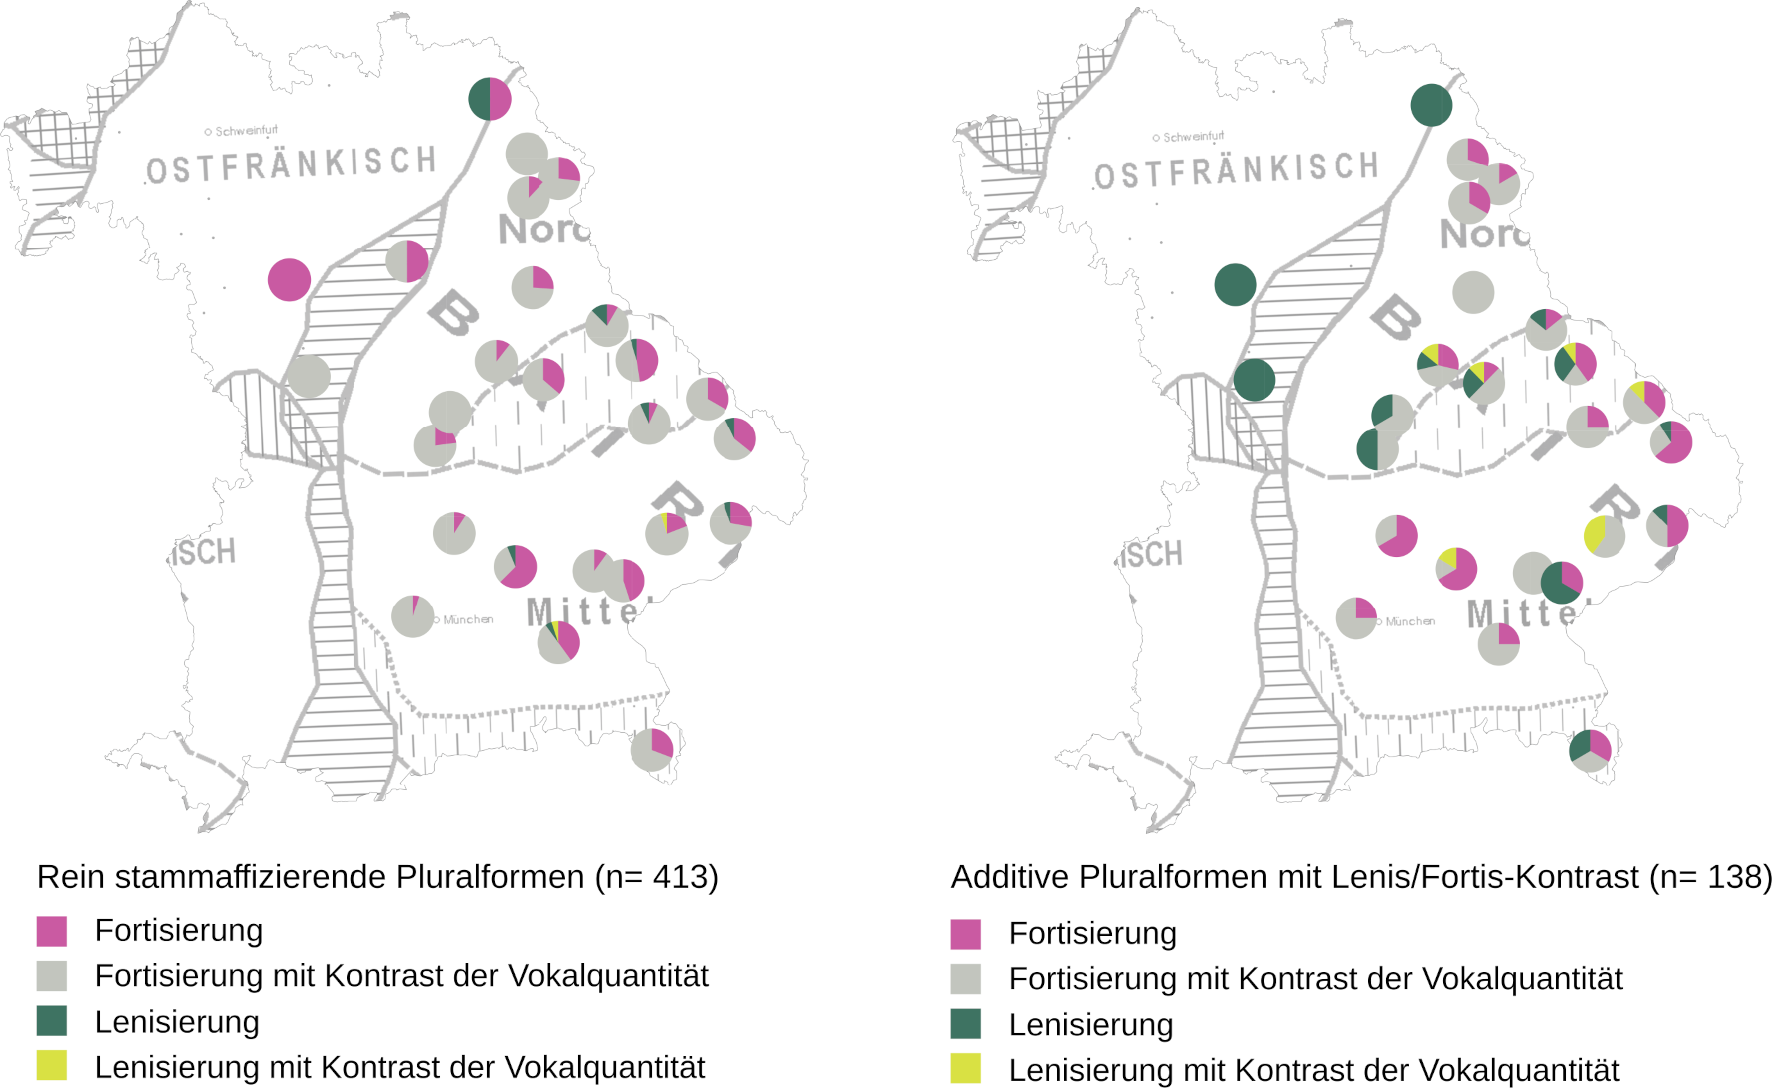
\includegraphics[width=\textwidth]{figures/Karte12.png}
\caption{Häufigkeitsverteilung innerparadigmatischer Lenis-Fortis-Kontraste im In- und Auslaut bei stammaffizierenden und additiven Pluralformen ($n=551$)}
\label{map:12}
\end{map}
\vfill\pagebreak

Tatsächlich zeigt die Gegenüberstellung von additiven und stammaffizierenden Verfahren, dass bei additiven Formen der Anteil an Lenes im Plural größer ist als in stammaffizierenden Pluralformen. Insbesondere im nordbair.-mittelbair. Übergangsgebiet, teilweise auch im Mittelbair. wird der Stammauslaut vor Nasalsuffix regelmäßig lenisiert (z.\,B. \teuthoo{An}{αn} \teuthoo{imp,\_}{imp͓ʰ} -- \teuthoo{imbqm}{imbʔm} ‚Imme‘ im nordbair.-mittelbair. Blaibach, \teuthoo{mu94<k,\_}{mu\klammeruntenpost{}̣̂k͓ʰ} -- \teuthoo{mu94<gán@}{mu\klammeruntenpost{}̣̂ɡ͈n̥} ‚Mücke‘ im mittelbair. Reischach). In einem Viertel der Lenisierungen entspricht die Korrelation von Vokal- und Konsonantismusquantität dabei dem bair. Silbengesetz, im Singular erscheint Kurzvokal+Fortis und im Plural Langvokal+Lenis, z.\,B. \teuthoo{A}{α} \teuthoo{tSe.3k}{tʃĕͅk} -- \teuthoo{tSe:<gn@}{tʃê{\doubleogonek}ɡn̥} ‚Zecke‘ im nordbair.-mittelbair. Blaibach. Insgesamt kann hier aber allenfalls von Tendenzen gesprochen werden, da sich für additive Pluralformen mit Nasalsuffix gleichermaßen Belege für Lenis im Singular und Fortis im Plural finden: \teuthoo{do<x1d}{dôx\⚬d} -- \teuthoo{do<x1t,n@}{dôx\⚬t͓n̥} ‚Docht‘ (ohne Quantitätskontrast) im nordbair.-mittelbair. Blaibach, \teuthoo{ho.<us\%}{hôͅus͈} -- \teuthoo{ho.uS,n@}{hoͅuʃ͓n̥} ‚Hase‘ (mit Quantitätskontrast) im mittelbair. Neukirchen am Inn. Daneben bietet \citet[§61.6]{Schießl1914} einen Hinweis darauf, dass die Lenis-Fortis-Alternation auch phonotaktisch bedingt sein kann: Im mittelbair. Dialekt von Eichendorf erscheint Fortis in der Verbindung Na\-sal+Den\-tal\-plo\-siv+Na\-sal „ausnahmslos“, das heißt, in additiven Pluralformen des Typs \textit{šd\~und} -- \textit{šd\~untn} ‚Stunde‘ oder in schwachen Akkusativ-Singular-Formen wie \textit{bl\~{\i}nd} -- \textit{ən bl\~{\i}ntn} ‚einen Blinden‘ ist Fortisplosiv durch die phonologische Umgebung gesteuert.

Auch bei den apokopierten Singularstammformen finden sich verschiedene Realisierungen der Vokal- und Konsonantenquantitätsverhältnisse und der Alternationsmuster, wie \tabref{tab:27} exemplarisch für drei Feminina im nordbair.-mittelbair. Übergangsgebiet illustriert: Während es für \textit{Brücke} und \textit{Straße}\footnote{Nach \citet[1093]{Wiesinger1983e} sind mhd. Langvokale wie mhd. \textit{â} in \textit{Straße} vor Frikativ- und Plosivgeminaten im Mittel- und Nordbair. sowie im Unterofr. regulär gekürzt worden.}  zum Teil innerparadigmatische Fortis/Lenis-Alternationen (teilweise auch in Korrelation mit der Vokalquantität) vor Nasalsuffix gibt, findet sich für \textit{Achse} kein innerparadigmatischer Wechsel. Interessant ist in diesem Zusammenhang außerdem, dass apokopierte Singularformen nur in der Tendenz, nicht aber grundsätzlich, Fortisauslaut aufweisen (dies modelliert die Tiefenstruktur /aksa/ vs. [aks] ‚Achse‘ nach \citealt[44]{Hinderling1980}), und sich verschiedene (Gegen-)Beispiele mit Konsonantismusalternation finden, z.\,B. \teuthoo{se).Nsd}{se\klammeruntenpost{}ͅŋsd} -- \teuthoo{se).Nst,-n@}{se\klammeruntenpost{}ͅŋst͓{}͐n̥} ‚Sense‘ im nordbair. Windischeschenbach und \teuthoo{bi.Agá\_}{biͅαɡ͈ʰ} -- \teuthoo{bi.AkAn}{biͅαkαn} ‚Birke‘ im mittelbair. Kirchensur.


\begin{table}
\begin{tabular}{lllll}
\lsptoprule
& {Singular} & {Plural} & {Diminutiv} & \\
\midrule
 ‚Achse‘ & \teuthoo{dqa4k,S}{dʔạk͓ʃ} & \teuthoo{dqa4kSn@}{dʔạkʃn̥} &  & Bernhardswald\\
& \teuthoo{a4<gðs5}{ậɡ̩s̩} & \teuthoo{a4<gðs5n@}{ậɡ̩s̩n̥} &  & Bernried\\
& \teuthoo{a4ks}{ạks} & \teuthoo{a4ksn@}{ạksn̥} &  & Blaibach\\
& \teuthoo{wo4<Na4kS}{wộŋạkʃ} & \teuthoo{wo4<Na4kSn@A}{wộŋạkʃn̥α} &  & Grafenkirchen\\
& \teuthoo{a4k,S,}{ạk͓ʃ͓} & \teuthoo{a4kSn@}{ạkʃn̥} &  & Zwiesel\\
\tablevspace
 ‚Brücke‘ & \teuthoo{bru.k,\_}{bruͅk͓ʰ} & \teuthoo{bru.gðn@}{bruͅɡ̩n̥} & \teuthoo{brigðl°@}{briɡ̩l̥̑} & Bernhardswald\\
& \teuthoo{brugá}{bruɡ͈} & \teuthoo{brugáAn}{bruɡ͈αn} & \teuthoo{brI.?gáAl}{brı̈ͅɡ͈αl} & Bernried\\
& \teuthoo{bru4k\_}{brụkʰ} & \teuthoo{bru.gðn@}{bruͅɡ̩n̥} & \teuthoo{bri4gðe4}{brịɡ̩ẹ} & Blaibach\\
& \teuthoo{bruk\_}{brukʰ} & \teuthoo{bru.kN@}{bruͅkŋ̥} & \teuthoo{brikl}{brikl} & Grafenkirchen\\
& \teuthoo{bruk\_}{brukʰ} & \teuthoo{bruk,An}{bruk͓αn} & \teuthoo{brI.?kAl}{brı̈ͅkαl} & Zwiesel\\
\tablevspace
 ‚Straße‘ & \teuthoo{s\#dra.S}{šdraͅʃ} & \teuthoo{s\#dra.2sn@}{šdrāͅsn̥} & \teuthoo{s\#dra4Sl.@}{šdrạʃl̥ͅ} & Bernhardswald\\
& \teuthoo{s\#5d5roS}{š̩d̩roʃ} & \teuthoo{s\#5d5ra4Sn@}{š̩d̩rạʃn̥} & \teuthoo{s\#5d5ra4SAl}{š̩d̩rạʃαl} & Bernried\\
& \teuthoo{s\#dra.S}{šdraͅʃ} & \teuthoo{s\#dra.Sn@}{šdraͅʃn̥} & \teuthoo{s\#dra4Sl@}{šdrạʃl̥} & Blaibach\\
& \teuthoo{s\#dra.S}{šdraͅʃ} & \teuthoo{s\#dra.Sn@}{šdraͅʃn̥} & \teuthoo{s\#dra4Sý@}{šdrạʃɫ̥} & Grafenkirchen\\
& \teuthoo{s\#d5ra:S}{šd̩ra{\doubleogonek}ʃ} & \teuthoo{s\#5d5ra.2sn@}{š̩d̩rāͅsn̥} & \teuthoo{s\#5d5ra4<s\%l@}{š̩d̩rậs͈l̥} & Zwiesel\\
\lspbottomrule
\end{tabular}
\caption{Exemplarische Beispiele apokopierter Singularformen -- Plural mit Nasalsuffix im nordbair.-mittelbair. Übergangsgebiet\label{tab:27}}
\end{table}

So heterogen das bisherige Bild bei CVC(C)-Einsilbern ist, so heterogen sind auch die Quantitätsverhältnisse bei zweisilbigen CVCV-Sequenzen, d.\,h. bei historischen Mehrsilbern. Auch hier findet sich vereinzelt ein Nebeneinander von Lenis- und Fortisalternanzen, z.\,B. \teuthoo{o):kA}{o\klammeruntenpost{}{\doubleogonek}kα} -- \teuthoo{a4gáA}{ạɡ͈α} ‚Acker‘ im nordbair.-mittelbair. Bernried vs. \teuthoo{o<.gáA}{ôͅɡ͈α} -- \teuthoo{a4<k,A}{ậk͓α} (neben \teuthoo{a4<gáA}{ậɡ͈α}) im mittelbair. Neukirchen am Inn, daneben gibt es vereinzelte Beispiele für Lenisierungen wie \teuthoo{ha4f,A}{hạf͓α} -- \teuthoo{ha4v\%An}{hạv͈αn} -- Dim. \teuthoo{ha4i.v\%e4}{hạiͅv͈ẹ} ‚Hafen‘ im mittelbair. Grafenau. Die Gegenüberstellung von exemplarischen Zweisilbern in den mittelbair. Tiefenbohrungspunkten (\tabref{tab:28}) zeigen einerseits, dass es Belege für die Kombination von Langvokal+Fortiskonsonanz (bei \textit{Mutter}) und von Kurz\-vo\-kal+Le\-nis\-kon\-so\-nanz (\textit{Apfel} in Inning am Holz und Neukirchen) in den Daten gibt (vgl. \citealt{MoosmüllerBrandstätter2014}). Anderseits gibt es Variation im Singularparadigma hinsichtlich der Vokalquantität (vgl. Nom. und Dat.Sg. von \textit{Mutter} in mittelbair. Kirchensur und Pasing) sowie zwischen Nom.Sg., Nom.Pl. bzw. Diminutivform hinsichtlich Lenis-Fortis-Konsonanz (vgl. \textit{Schwester} im mittelbair. Inning am Holz und Neukirchen sowie \textit{Apfel} in Inning am Holz).

\begin{table}[p]
\begin{tabularx}{\textwidth}{llQQl}
\lsptoprule
& {Nom.Sg.} & {Nom.Pl.} & {Dat.Sg.} & \\
\midrule
 ‚Mutter‘ & \teuthoo{b-mu.<AtE}{b{}͐mûͅαtə} & \teuthoo{b-mîiAtE@}{b{}͐m{\aufstrih}iαtə̥} &  & Inning am Holz\\
& \teuthoo{b5muAtA}{b̩muαtα} & \teuthoo{muAtAn}{muαtαn} & \teuthoo{A}{α} \teuthoo{dA}{dα} \teuthoo{mu<AtA}{mûαtα} & Kirchensur\\
& \teuthoo{b-mu.<AtE}{b{}͐mûͅαtə} & \teuthoo{mu94<AtEn}{mu\klammeruntenpost{}̣̂αtən} & \teuthoo{dA4mu4<AtEn}{dα̣mụ̂αtən} & Neukirchen am Inn\\
& \teuthoo{b\_mu.<AtA}{bʰmûͅαtα} & \teuthoo{mu.AtAn}{muͅαtαn} & \teuthoo{A}{α} \teuthoo{dA}{dα} \teuthoo{mu.<AtAn}{mûͅαtαn} & Niedertaufkirchen\\
& \teuthoo{b5\_mu.AtA}{b̩ʰmuͅαtα} & \teuthoo{miAtA}{miαtα} & \teuthoo{dA}{dα} \teuthoo{mu.<AtA}{mûͅαtα} & Pasing\\
& \teuthoo{b5mu.AtA}{b̩muͅαtα} & \teuthoo{bmi.AtA}{bmiͅαtα} & \teuthoo{dA}{dα} \teuthoo{muAtA}{muαtα} & Wolfersdorf\\
\tablevspace
 ‚Schwester‘ & \teuthoo{mâa4<e+}{m{\aufstrih}ậẽ} \teuthoo{s\#wes\%t,A4}{šwes͈t͓α̣} & \teuthoo{ma4<i.ne}{mậiͅne} \teuthoo{s\#we4S,t;An}{šwẹʃ͓t͓͓αn} &  & Inning am Holz\\
& \teuthoo{ma4<e<}{mậê} \teuthoo{s\#we4Sd5A}{šwẹʃd̩α} & \teuthoo{ma4<e<ne4}{mậênẹ} \teuthoo{s\#we4Sd5An}{šwẹʃd̩αn} &  & Kirchensur\\
& \teuthoo{ma4i:}{mai{\doubleogonek}} \teuthoo{s\#wes\%d\%A}{šwes͈d͈α} & \teuthoo{ma4<i.ne}{mậiͅne} \teuthoo{s\#wes\%t;En}{šwes͈t͓͓ən} &  & Neukirchen am Inn\\
& \teuthoo{ma4<e4}{mậẹ} \teuthoo{s\#we4s5t,A}{šwẹs̩t͓α} & \teuthoo{ma4e4ne4}{mạẹnẹ} \teuthoo{s\#we4s5tAn}{šwẹs̩tαn} &  & Niedertaufkirchen\\
& \teuthoo{m{\textasciitilde}ôe.<I:}{m{\aufstrih}êi{\doubleogonek}} \teuthoo{s\#we4Sd\%A}{šwẹʃd͈α} & \teuthoo{m{\textasciitilde}ôe.>(+i:(6nîi:}{m{\aufstrih}êi{\doubleogonek}n{\aufstrih}i{\doubleogonek}}
 \teuthoo{s\#we4Sd\%An}{šwẹʃd͈αn} &  & Pasing\\
& \teuthoo{mâa4>(+e>(+}{m{\aufstrih}ậ̃\klammerobenpost{}ễ\klammerobenpost{}} \teuthoo{s\#we4Sd5A}{šwẹʃd̩α} & \teuthoo{ma4+e+ne4}{mạ̃ẽnẹ} \teuthoo{{s\#we4Sd5A}n}{šwẹʃd̩αn} &  & Wolfersdorf\\
\midrule & Nom.Sg. & Nom.Pl. & Diminutiv & \\\midrule
 ‚Apfel‘ & \teuthoo{o4b5v\%e}{ọb̩v͈e} & \teuthoo{e4<b5v\%e}{ệb̩v͈e} & \teuthoo{e4b\%fAl}{ẹb͈fαl} & Inning am Holz\\
& \teuthoo{o4pfe4}{ọpfẹ} & \teuthoo{e4pfe4}{ẹpfẹ} & \teuthoo{a4pfAl}{ạpfαl} & Kirchensur\\
& \teuthoo{ob5v\%e}{ob̩v͈e} & \teuthoo{e94bv\%e?}{e\klammeruntenpost{}̣bv͈ë} & \teuthoo{a4b\%v\%Al}{ạb͈v͈αl} & Neukirchen am Inn\\
& \teuthoo{o4pfe4}{ọpfẹ} & \teuthoo{e4pfe4}{ẹpfẹ} & \teuthoo{a4pfAl}{ạpfαl} & Niedertaufkirchen\\
& \teuthoo{a.pfîi:}{aͅpf{\aufstrih}i{\doubleogonek}} & \teuthoo{e4pfîi:}{ẹpf{\aufstrih}i{\doubleogonek}} & \teuthoo{a4pfAl°}{ạpfαl̑} & Pasing\\
& \teuthoo{a:pfe4}{a{\doubleogonek}pfẹ} & \teuthoo{e4pfe4}{ẹpfẹ} & \teuthoo{a4pfAl}{ạpfαl} & Wolfersdorf\\
\lspbottomrule
\end{tabularx}
\caption{Quantitätsverhältnisse in CVCV-Strukturen in den mittelbair. Tiefenbohrungspunkten (Auswahl)\label{tab:28}}
\end{table}

Anhand dieses exemplarischen Blicks in die BSA-Daten wird deutlich, dass für die Analyse -- neben der (morpho)phonologischen Ebene -- notwendigerweise die Ebene der Transkription berücksichtigt werden muss. Teilweise bestehen die Lenis-Fortis-Kontraste in nur einem Segment einer Konsonantensequenz, teilweise nur in der Abstufung der Diakritika, vgl. \teuthoo{no.2Xd}{nōͅꭗd} -- \teuthoo{na4x5d\%}{nạx̩d͈} ‚Nacht‘ im mittelbair. Pasing (vgl. die Typisierungsprinzipien in \sectref{sec:6.3.1.2}).\footnote{\citet[13]{Schießl1909} zeigt der in seiner phonetischen Darstellung des mittelbair. Dialekts von Eichendorf, dass Lenis-Fortis-Kontraste bei Velarfrikativ [x] durch die weniger starke „Reibeenge“ weniger deutlich ausfallen als bei den übrigen Frikativen oder bei Plosiv, demnach können zudem unterschiedlich starke Kontraste für die einzelnen konsonantischen Artikulationsarten angenommen werden.} Artikulation findet eben nicht in Form binärer phonologischer Oppositionen, sondern als Ausprägungen einer kontinuierlichen Skala statt; die Teuthonista als sehr fein abgestuftes Transkriptionssystem dokumentiert diese z.\,T. minimalen phonetischen Unterschiede. So sieht auch \citet[22]{Scheutz1984} als Ergebnis seiner Quantitätsmessungen „die eher kontinuierliche als streng dichotomische Skalierung der Quantitätsverhältnisse“ als „ein kaum zu leugnendes Faktum“ an. Dies wurde auch während der Exploration des \textit{Bayerischen Sprachatlas} beobachtet, wie ein Blick in den Einführungsband des SNiB zeigt:

\begin{quote}
Insgesamt wurde im Erhebungszeitraum außerdem festgestellt, dass die Bestimmung der Vokalquantitäten, vor allem vor Frikativ oder Nasalkonsonant oft sehr schwierig ist. Der damit in Zusammenhang stehende Gegensatz von Lenis-Fortis ist oft nicht eindeutig. Die tatsächliche Realisierung verstößt häufig gegen die ‚bairische Gesetzmäßigkeit‘ von Fortes nach Kurzvokal, Lenes nach Langvokal und Diphthongen. (\citealt[23]{SNiB1})\footnote{Vgl. auch \citet[405--406]{Götz1987} zu Schwierigkeiten der Transkription der bair. Quantitätsverhältnisse.}
\end{quote}

Eine Auswertung von innerparadigmatischen Quantitätskontrasten in den Daten des BSA kann nicht losgelöst von methodischen Spezifika der BSA-Daten stattfinden, die morphophonologische Analyse ist zunächst immer an die phonetische Ebene gekoppelt. Darüber hinaus ist die Lenis-Fortis-Alternation aus morphophonologischer Sicht auch deshalb besonders interessant, weil sie im Mittelbair. „gewissermaßen ein Doppelleben“ \citep[191]{Seiler2008} führt: Sie ist sowohl morpho(phono)logisch als auch phonologisch konditioniert, selbst wenn entsprechende Lenis-Fortis-Alternationen synchron lexikalisiert und nicht das Ergebnis eines produktiven phonologischen Prozesses sein sollten (vgl. \citealt[19]{Scheutz1984}).

\subsubsubsubsection{Lenis-Fortis-Kontraste zwischen Lexikalisierung und Produktivität}


Das hohe Maß an phonetischer Variation, die sich für die bair. Daten insgesamt und auch innerhalb der einzelnen Tiefenbohrungspunkte zeigt (vgl. die vorgestellten instrumentalphonetischen Studien sowie die exemplarischen Beispiele in 	\tabref{tab:28}), hat wiederum Auswirkungen auf die Modellierung als morphophonologisches Verfahren. Die Analyse der BSA-Daten zeigt hier, in welchem Maße Morphologie an Phonetik und Phonologie gebunden ist, und wie Sprecher des Bair. (morpho)phonologische Oppositionen als Pluralmarkierungsstrategien nutzen. So finden sich in den Daten Belege, dass Lenis-Fortis-Kontraste im UG als Pluralmarkierungsstrategie (teilweise in Kombination mit Kontrasten der Vokalquantität) im bair. Teil des UGs morphologisiert sind. \tabref{tab:29} zeigt zunächst innerparadigmatische Alternationen bei zweisilbigen CVCV-Segmenten auf.


\begin{table}
\begin{tabularx}{\textwidth}{lllQ}
\lsptoprule
{Singular} & {Plural} & {Diminutiv} & \\
\midrule
 \teuthoo{o4<b5v5l°@}{ộb̩v̩l̥̑} & \teuthoo{epfl°@n@}{epf‌l̥̑n̥} &  & ‚Apfel‘ (nordbair.-mittelbair. Bernhardswald)\\
 \tablevspace
 \teuthoo{goAd\%-n@}{ɡoαd͈n̥} & \teuthoo{ga4rt-n@}{ɡạrt͐n̥} & \teuthoo{ga4rtl@}{ɡạrtl̥} & ‚Garten‘ (nordbair.-mittelbair. Zwiesel)\\
 \tablevspace
 \teuthoo{ha4<gðl@}{hậɡ̩l̥} & \teuthoo{ha4k;l@n}{hạk͓͓l̥n} & \teuthoo{ha4<gAl}{hậɡαl} & ‚Haken‘ (mittelbair. Neukirchen am Inn) \\
 \tablevspace
 \teuthoo{mu<g-N@}{mûɡ{}͐ŋ̥} & \teuthoo{muk-N@}{muk{}͐ŋ̥} &  & ‚Mücke‘ (mittelbair. Grafenau)\\
 \tablevspace
 \teuthoo{bmu<EdA}{bmûədα} & \teuthoo{mutEn}{mutən} &  & ‚Mutter‘ (nordbair.-mittelbair. Grafenkirchen)\\
 \tablevspace
 \teuthoo{o4<v\%A}{ộv͈α} & \teuthoo{e4<f;A}{ệf͓͓α} &  & ‚Ofen‘ (nordbair. Oberdolling)\\
 \tablevspace
 \teuthoo{s\#u.b\%v\%A}{šuͅb͈v͈α} & \teuthoo{d5s\#5u.pfAn}{d̩š̩uͅpfαn} &  & ‚Schupfen‘ (mittelbair. Grafenau)\\
 \tablevspace
 \teuthoo{do94Xd\%A}{do\klammeruntenpost{}̣ꭗd͈α} & \teuthoo{d5e.Xt,A4}{d̩eͅꭗt͓α̣} &  & ‚Tochter‘ (mittelbair. Inning am Holz)\\
 \tablevspace
 \teuthoo{wu.(<Ed5s5ý@}{wûͅ\klammerobenpost{}əd̩s̩ɫ̥} & \teuthoo{wi.Et,S,ý@}{wiͅət͓ʃ͓ɫ̥} &  & ‚Wurzel‘ (nordbair. Groschlattengrün)\\
\lspbottomrule
\end{tabularx}
\caption{Lenis-Fortis-Kontraste in CVCV-Strukturen}
\label{tab:29}
\end{table}

Belege wie diese finden sich in vorhandenen Dialektdarstellungen kaum (vgl. \textit{Schindel} -- \textit{Schindtl} ‚Schindel‘ für das nordbair. Muttersdorf bei \citealt{Micko1933}, zitiert nach \citealt[123]{Rowley1997}). \citet[123]{Rowley1997} etwa kann in seinen nordostbayerischen Daten keine Belege für eine Morphologisierung des Lenis-Fortis-Kontrasts finden. Und auch in den vorliegenden Daten handelt es sich um einzelne Belege dieser Pluralmarkierungsstrategie für die jeweiligen Lexeme,\footnote{Für \textit{Mutter} ist in Blaibach und Bernhardswald (nordbair.-mittelbair. Übergangsgebiet) Lenisierung belegt: \teuthoo{bmuAtA}{bmuαtα} -- \teuthoo{muAdAnA}{muαdαnα} (Blaibach), \teuthoo{muEt,E}{muət͓ə} -- \teuthoo{mu<EdAnE}{mûədαnə} (Bernhardswald).} sodass sich nicht sagen lässt, ob es sich um lexikalisierte Formen handelt oder ob die Gewährspersonen sie spontan in Form von kumulierten Markierungsstrategien realisierten. (Nur im Fall von \teuthoo{mu<g-N@}{mûɡ{}͐ŋ̥} -- \teuthoo{muk-N@}{muk{}͐ŋ̥} ‚Mücke‘ im mittelbair. Grafenau besteht der formale Unterschied einzig im Quantitätenkontrast, die Alternative wäre damit Nullplural.)

Neben den Lenis-Fortis-Alternationen bei zweisilbigen CVCV-Stämmen gibt es in den Daten Belege eines morphologisierten Verfahrens für historische Einsilber. Die Wechsel sind insofern „unvoraussagbar“ \citep[46]{Hinderling1980}, als sie (in der Terminologie Hinderlings) historische „Lenislexeme“ betreffen, für die die Alternation nicht infolge eines (diachronen oder synchronen) phonetisch-phonologischen Prozesses entstanden ist, z.\,B. -- bei historischem Langvokal -- \teuthoo{ma<os}{mâos} -- \teuthoo{ma<iS}{mâiʃ} (nordbair. Tirschenreuth) und \teuthoo{ma(<4u.s5}{mâ\klammerobenpost{}̣uͅs̩} -- \teuthoo{ma43i.S}{mặiͅʃ} ‚Maus‘ (nordbair. Windischeschenbach).\footnote{\citet[329]{Zehetner1983} zählt für den Freisinger Stadtdialekt synchron auch \textit{Hut} zu den Lenisstämmen, da die Leniskonsonanz auch in anderen Stammformen erhalten ist, \textit{Huad} -- \textit{Hiad} neben Dim. \textit{Hiadal}. Folgt man dieser synchronen Klassifikation, gibt es in den vorliegenden Daten auch für diesen Lenisstamm analoge Lenis-Fortis-Kontraste im Nordbair. und nordbair.-mittelbair. Übergangsgebiet, z.\,B. \teuthoo{hôo.ud}{h{\aufstrih}oͅud} -- \teuthoo{hôe.it}{h{\aufstrih}eͅit} (nordbair. Nabburg).} Für die Alternation bei \textit{Maus} finden sich in den SNOB-Roh\-da\-ten weitere Belege im nördlichen Nordbair., sodass die kumulierte Pluralmarkierungsstrategie in diesem Gebiet tatsächlich lexikalisiert zu sein scheint (vgl.  \mapref{map:9} zu Quantitätskontrasten altem Langvokal oder Diphthong).


\begin{map}
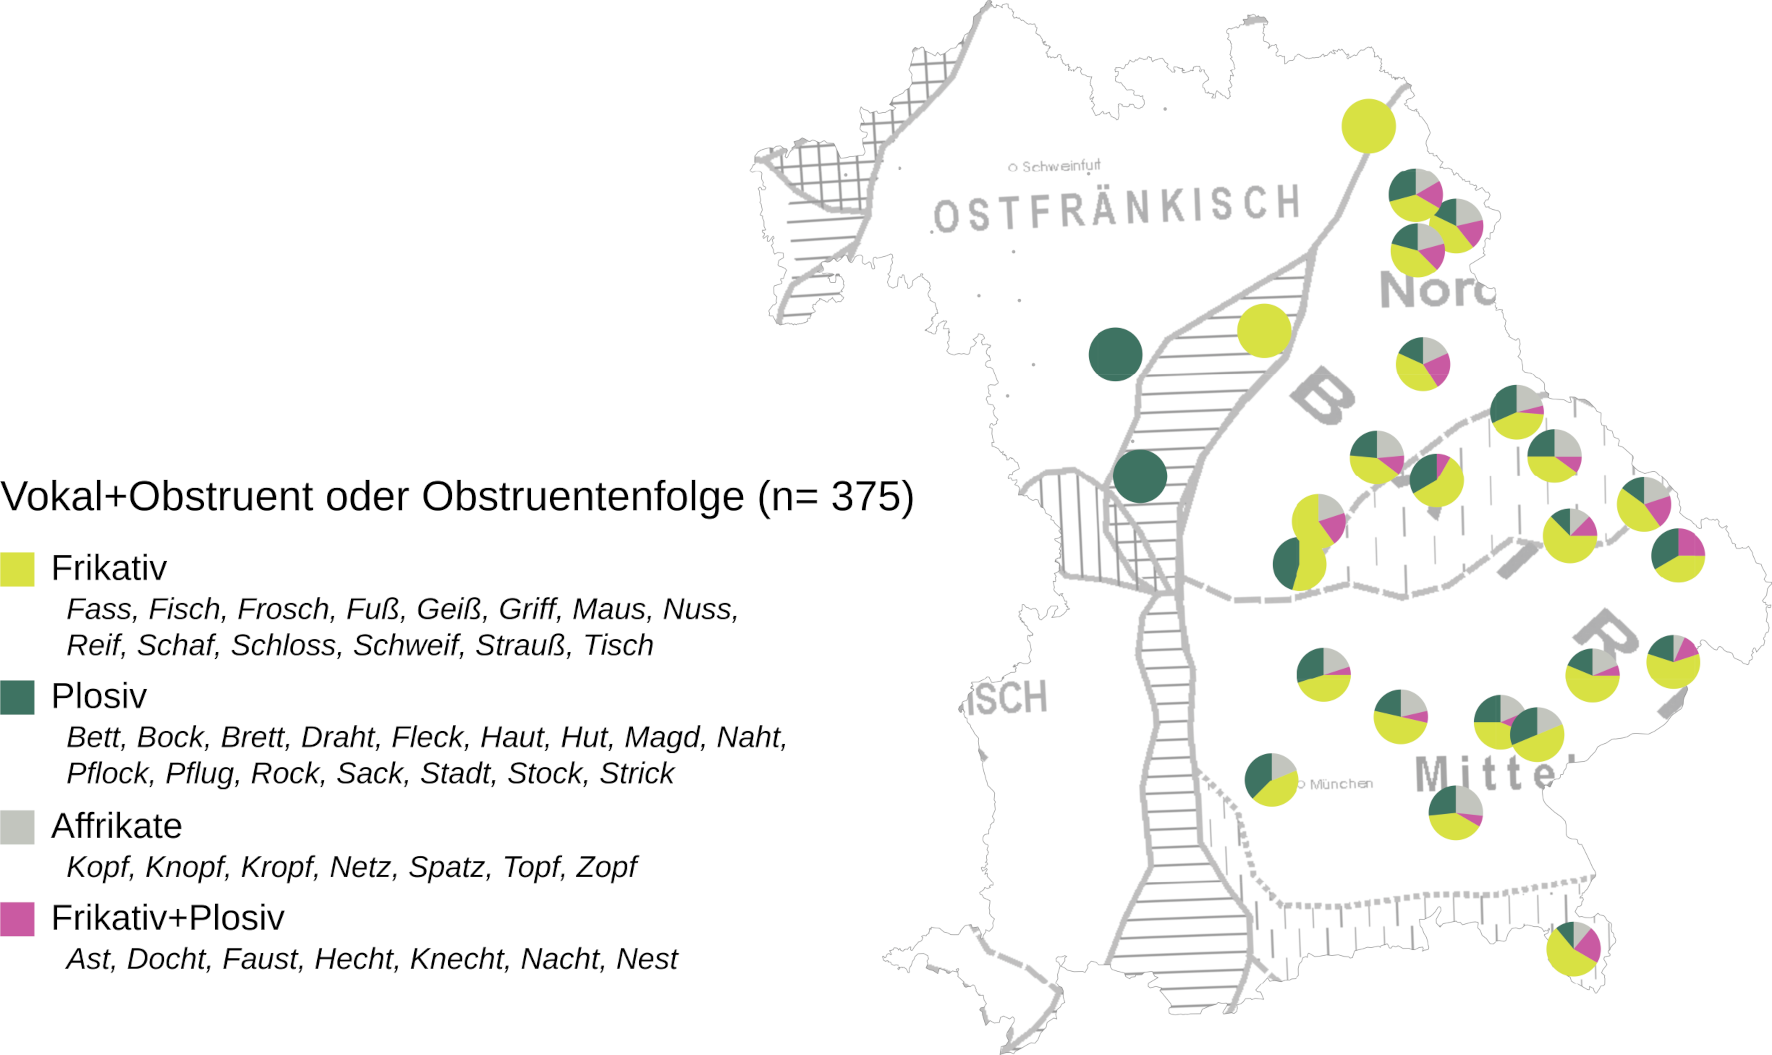
\includegraphics[width=\textwidth]{figures/Karte13.png}
\caption{Lenis-Fortis-Kontraste in Einsilbern in verschiedenen phonologischen Umgebungen}
\label{map:13}
\end{map}

Eine differenzierte Analyse von Leniskonsonanz im Singular und Fortiskonsonanz im Plural bei historischen Einsilbern zeigt darüber hinaus, dass die innerparadigmatische Alternation (respektive deren Fehlen) durch die Konsonanz (Einzelkonsonant oder Konsonantenfolge) des Auslauts bedingt sein kann (\mapref{map:13}). Lenis-Fortis-Kontraste finden sich in den verschiedenen (teilweise auch allen) phonologischen Umgebungen in den nördlichen nordbair. Tiefenbohrungspunkten. Die mittelbair. Ortspunkte und jene des nordbair.-mittelbair. Übergangsgebietes weisen insgesamt größere Unterschiede auf, da die innerparadigmatische Alternation hier nicht für sämtliche Konsonantenarten oder bei Konsonantenverbindungen belegt ist.\footnote{So finden sich beispielsweise im nordbair. Riedenburg keine Alternationen bei Plosiven, in verschiedenen mittelbair. Tiefenbohrungspunkten finden sich keine Belege für Alternationen bei Dental- oder Velarplosiv. Vereinzelt weisen Tiefenbohrungspunkte Alternation für Konsonantenfolgen, aber keine Alternation bei Affrikaten auf (mittelbair. Grafenau, nordbair.-mittelbair. Bernhardswald). Bemerkenswert ist, dass im nordbair. Oberdolling systematisch keine Lenis-Fortis-Kontraste bei Konsonantenfolgen erscheinen, bei Einzelkonsonanten aber sämtliche Obstruenten belegt sind.}

Auf der Lexemebene sind bei Einsilbern mit Vokal-Obstruent-Abfolge regionale Schwankungen zu beobachten, die v.\,a. durch lexemspezifische Entwicklungen bedingt sind. Einzelne Lexeme haben großräumige Geltung, andere sind nur in einem kleineren Gebiet oder vereinzelt belegt:

\begin{itemize}\sloppy
\item Bei den Frikativen sind großräumig \textit{Schweif}, \textit{Reif}, \textit{Griff}; \textit{Fuß}, \textit{Geiß}, \textit{Schloss} und \textit{Fisch}, \textit{Frosch}, \textit{Tisch} belegt, im Nordbair. finden sich daneben \textit{Fass}, \textit{Strauß}.
\item Lenis-Fortis-Kontrast bei Plosiv findet sich großräumig für \textit{Haut}, \textit{Sack}, \textit{Stock}, \textit{Rock}, vereinzelt im Nordbair und im nordbair.-mittelbair. Übergangsgebiet \textit{Bett}, \textit{Hut} und \textit{Stadt}.
\item Lenis-Fortis-Kontraste in wortfinalen Konsonantenclustern haben für die Abfolge /st/ in \textit{Ast}, \textit{Faust} großräumige Geltung (vereinzelt findet sich \textit{Fest}). /xt/ ist im Nordbair. teilweise belegt für \textit{Docht} und \textit{Hecht} und im gesamten bair. UG vereinzelt bei \textit{Nacht} und \textit{Knecht} (vgl. \citealt[33]{Hinderling1980}, \citealt[119]{Seiler2005}).\footnote{In Liquid-Obstruent-Abfolgen, die hier nicht kartiert wurden, finden sich vereinzelt Fortisierungen bei \textit{Bild}, \textit{Feld}, \textit{Holz} und \textit{Wald} im Nordbair. Großräumig im Nord- und Mittelbair. finden sich Lenis-Fortis-Kontraste in /r/-Obstruent-Abfolgen bei \textit{Dorf}, vereinzelt bei \textit{Wirt}, \textit{Markt}, \textit{Korb}, \textit{Herz} (jeweils mit vokalisiertem /r/).}
\item Die Affrikaten /pf/ und /ts/ sind großräumig für \textit{Knopf}, \textit{Kropf}, \textit{Zopf} und vereinzelt \textit{Topf} und \textit{Netz} im Nordbair. bzw. nordbair.-mittelbair. Übergangsgebiet belegt.
\end{itemize}

Systematisch neutralisiert ist nach \citet[45]{Zehetner1978} „die Wirkkraft“ des sogenannten Bair. Silbengesetzes in Abfolgen aus /r/+Obstruent und auch bei Nasal+Obstruent, es finden sich Kombinationen von Kurzvokal und Leniskonsonanz (vgl. \citealt{Hinderling1980}: 28). Laut \citet[123]{Rowley1997} besteht im südlichen Nordbair. der formale Unterschied zwischen Singular- und Pluralform in Nasal-Obstruent-Abfolgen einzig im Lenis-Fortis-Kontrast. Dieser Befund findet sich in den vorliegenden Daten in einzelnen Ortsdialekten des Nord- und Mittelbair. wieder: Im mittelbair. Kirchensur und im nordbair. Tirschenreuth gibt es keine Belege für Vokalquantitätskontraste vor Nasal+Obstruent in historischen Einsilbern, daneben werden auch in anderen mittelbair. und teilweise nordbair. Tiefenbohrungspunkten innerparadigmatische Kontraste vor Nasal+Obstruent nur in Form von Lenis-Fortis-Kontrasten realisiert, z.\,B. \teuthoo{s\#wa.nds5}{šwaͅnds̩} -- \teuthoo{s\#wa4ntS}{šwạntʃ} ,‚Schwanz‘ (mittelbair. Kirchensur) und \teuthoo{A}{α} \teuthoo{hund}{hund} -- \teuthoo{hunt\_}{huntʰ} -- Dim. \teuthoo{hund5Al}{hund̩αl} ‚Hund‘ (nordbair.-mittelbair. Blaibach). Insgesamt scheint es sich aber v.\,a. um lexemspezifische Entwicklungen zu handeln. So sind \textit{Hund} und \textit{Strumpf} ohne Quantitätskontraste in Ortspunkten belegt, die Quantitätskontraste bei anderen Lexemen (z.\,B. \textit{Schwanz} und \textit{Band}) aufweisen.

Damit zeigt die Auswertung der einzelnen Obstruenten und Konsonantenabfolgen im Auslaut der Singularform, dass die phonologische Umgebung eine Variable ist, die für jeden Ortsdialekt bedingt, ob innerparadigmatische Quantitätskontraste (von Vokal und/oder Obstruent) im System des Ortsdialekts als Pluralmarkierungsstrategie zur Verfügung stehen. Daneben scheint die Art des Kodierungsverfahrens häufig lexemspezifisch zu sein.


\begin{figure}
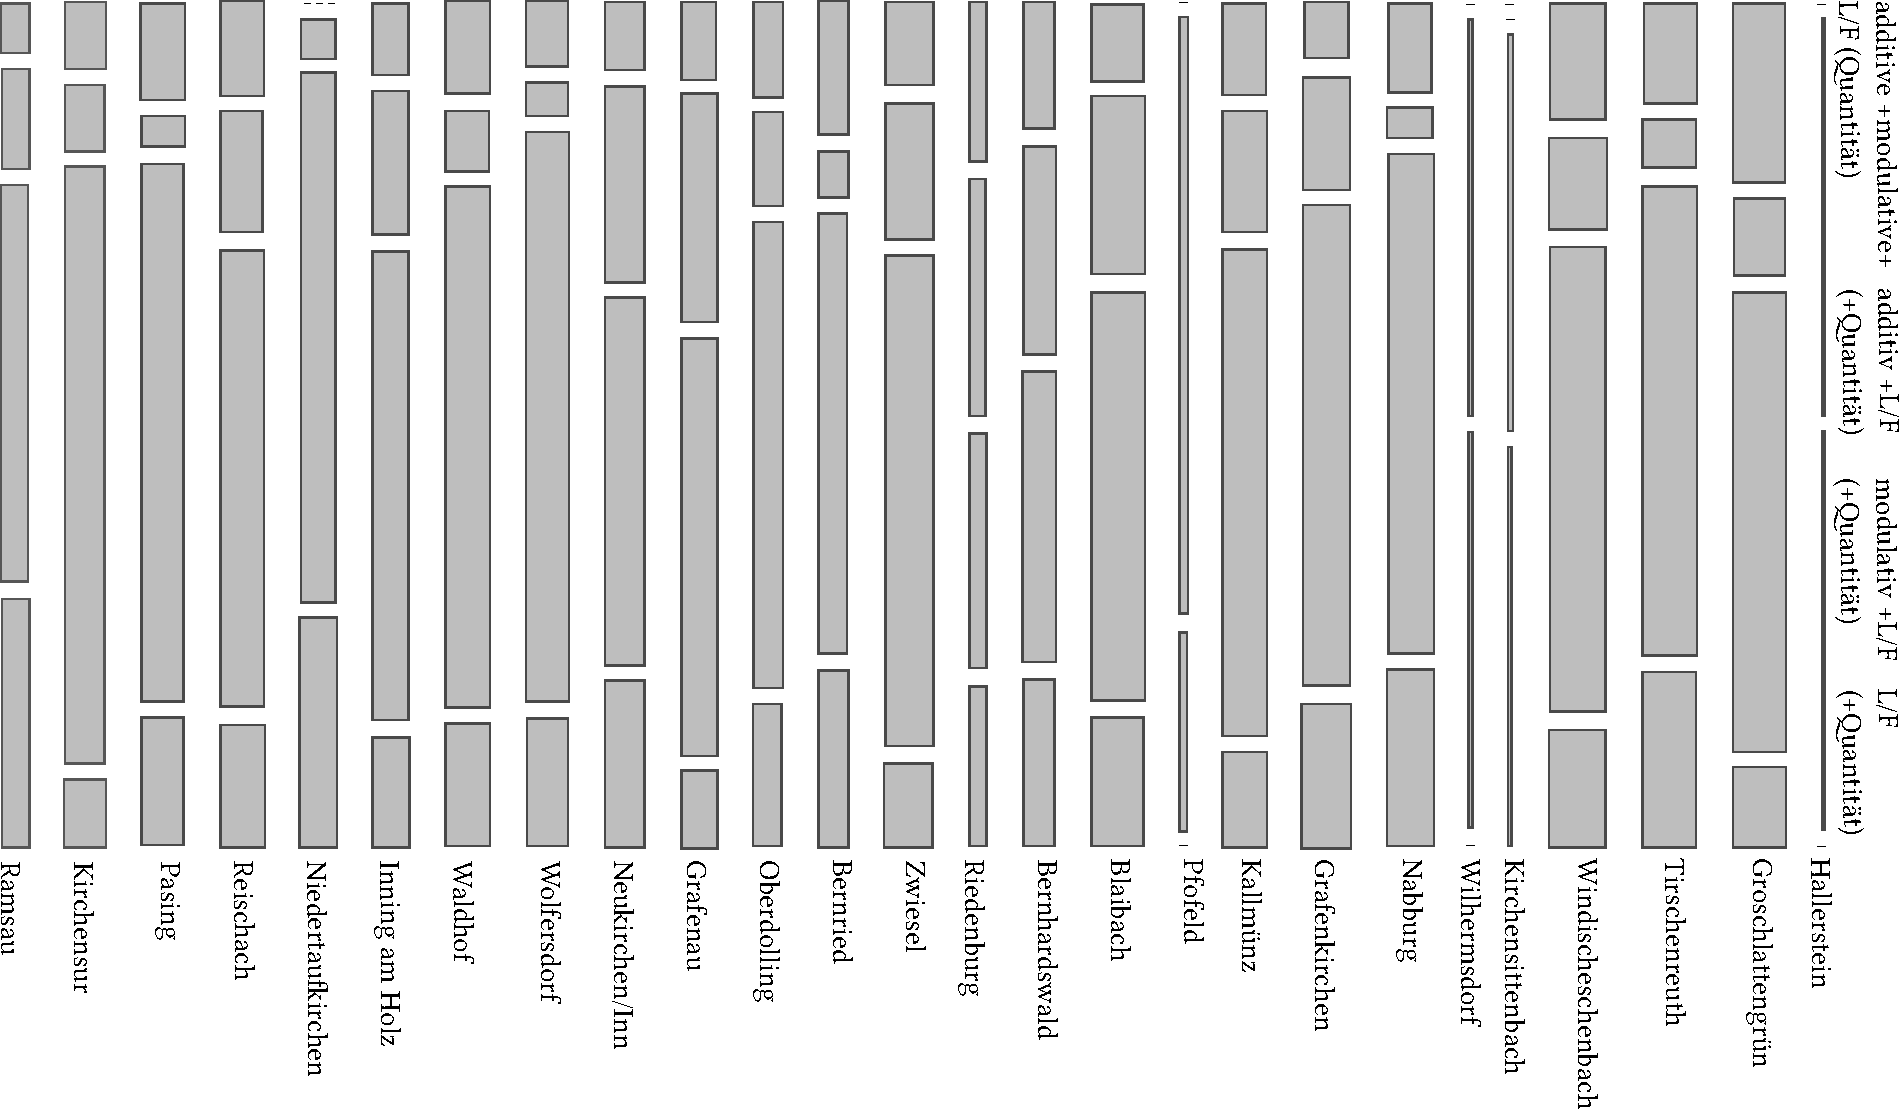
\includegraphics[height=0.75\textwidth, angle=90]{figures/revisedNickelNominalmorphologie-img022.pdf}
\caption{Mosaik-Plot mit Häufigkeitsverteilung von Lenis-Fortis-Kontrasten (L/F) in Kombination mit anderen additiven und stammaffizierenden Verfahren ($n=508$)}
\label{fig:6}
\end{figure}

Lenis-Fortis-Kontraste erscheinen als kumulative Pluralmarkierungen vor allem in Kombination mit Kontrasten der Vokalqualität als weiterem stammaffizierenden Verfahren, wie das Mosaik-Plot in  \figref{fig:6} für alle Tiefenbohrungspunkte mit Lenis-Fortis-Kontrasten illustriert. Das Mosaik-Plot visualisiert die Variablen Ortsdialekt (von Nord nach Süd), Typus des Pluralverfahrens und absolute Häufigkeit. Anhand der Größe der Flächen der Rechtecke ergibt sich, dass die Vorkommenshäufigkeit in den Dialekten schwankt, in den ofr. Ortsdialekten handelt es sich um ein nur peripheres Phänomen. Das Plot zeigt zudem, dass die relative Häufigkeit von Lenis-Fortis-Kontrasten in Kombination mit einem additiven Verfahren in den einzelnen Ortsdialekten z.\,T. stark schwankt, es überwiegen Kombination aus additiv-modulativer Markierung und Quantitätskontrasten. Innerhalb des Nord- und Mittelbair. scheint es hier ortsdialektspezifische Präferenzen zu geben, in welchem Umfang und in welcher Kombination innerparadigmatische Lenis-Fortis-Kontraste als Kodierungsverfahren im Flexionssystem den Sprechern zur Verfügung stehen.

An dieser Stelle ist eine Vorausschau auf Genus als möglichem Konditionierungsfaktor der Deklinationsklassenzugehörigkeit sinnvoll, da die Unterschiede im Mosaik-Plot hinsichtlich der Präferenz einzelner Markierungsstrategien für die Ortsdialekte durch Genus bedingt sind (ausführlicher \sectref{sec:8.3.1}). \mapref{map:14} visualisiert für die areale Dimension die Häufigkeitsverteilung
von Lenis-Fortis-Kontrasten nach Genus differenziert. In allen Ortspunkten sind innerparadigmatische Lenis-Fortis-Kontraste am häufigsten für Maskulina belegt. Dieser Typus von Konsonantismusalternationen ist in den rezenten Dialekten in der Tendenz ein spezifisch maskulines Verfahren, was primär durch die historische Deklinationsklassenzugehörigkeit bedingt ist (vgl. \sectref{sec:8.2.1}). Unterschiede zwischen den Ortspunkten ergeben sich v.\,a. durch unterschiedliche Anteile von Feminina und Neutra. Das mittelbair. Grafenau etwa sticht mit einem vergleichsweise hohen Anteil an Feminina heraus. Der Blick in die Daten zeigt, dass hier Lenis-Fortis-Kontraste nicht nur bei Feminina der historischen \textit{i}{}-Deklination belegt sind, sondern auch in CVCV-Strukturen produktiv ist (z.\,B. \teuthoo{mu<g-N@}{mûɡ{}͐ŋ̥} -- \teuthoo{muk-N@}{muk{}͐ŋ̥} ‚Mücke‘, vgl. 	\tabref{tab:29}).

\begin{map}[p]
\centering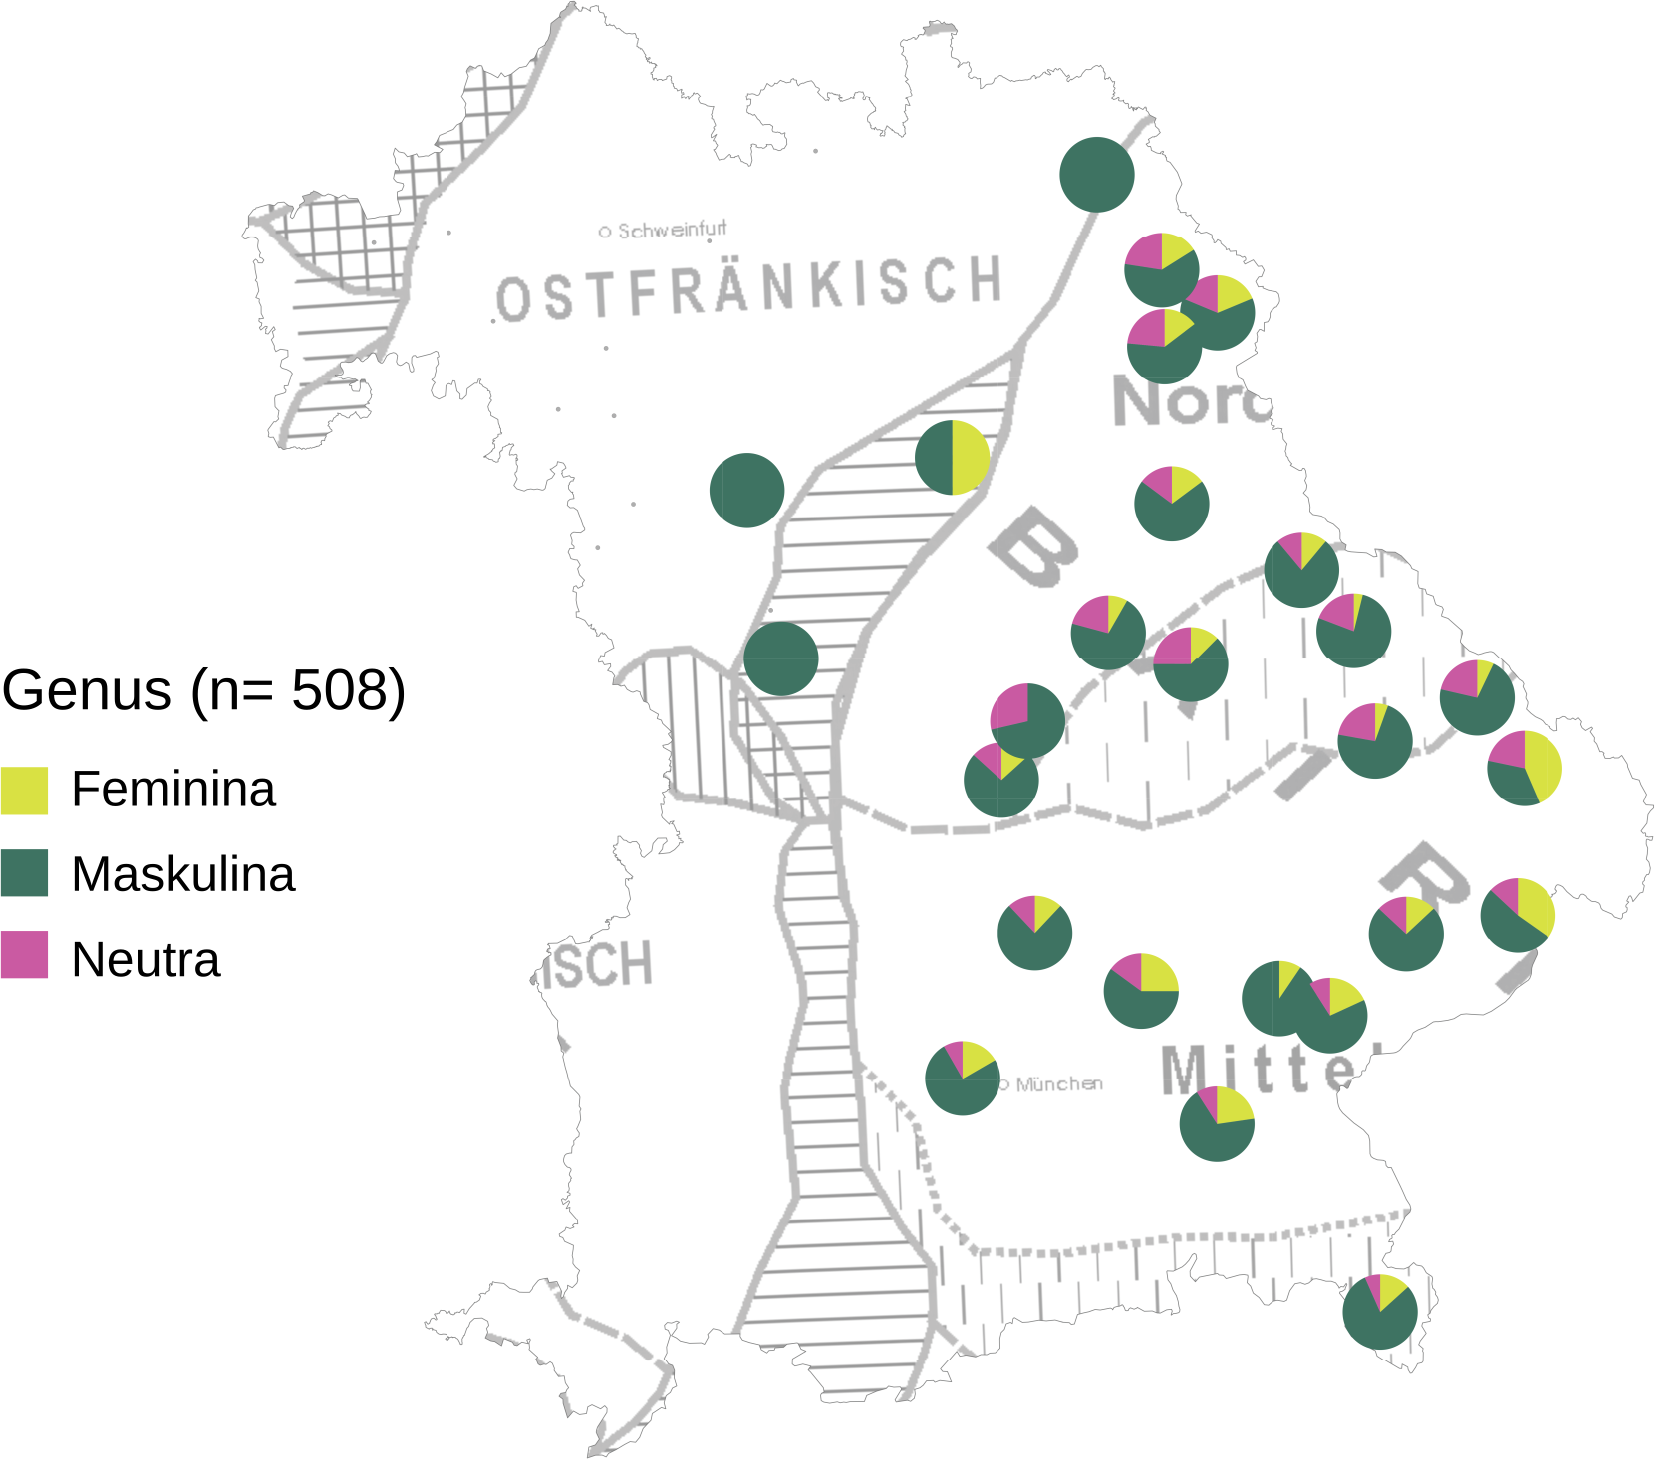
\includegraphics[width=.8\textwidth]{figures/Karte14.png}
\caption{Häufigkeitsverteilung der Lenis-Fortis-Kontraste für die Genera}
\label{map:14}
\end{map}

\begin{table}[p]
\begin{tabular}{lrrr}
\lsptoprule
     &  Maskulinum & Femininum & Neutrum\\
     \midrule
     add/kons/quant & 6 & 16 & 25\\
     add/mod/kons/quant & 4 & 2 & 54\\
     kons/quant & 79 & 9 & 0\\
     mod/kons/quant & 260 & 53 & 0\\
     \lspbottomrule
\end{tabular}
\caption{Korrespondenzanalyse der Variablen Genus und Pluralmarkierungsverfahren ($n=507$)}
\label{tabfig:7}
\end{table}


Dass die Wahl des Kodierungsverfahrens primär durch Genus konditioniert ist, illustriert auch die Korrespondenzanalyse in  \figref{fig:7} und \tabref{tabfig:7}.\footnote{Diese und folgende Korrespondenzanalysen wurden erstellt mit dem R-Paket \textit{languageR} von Harald Baayen (vgl. \citealt{Baayen2015}, \url{https://www.rdocumentation.org/packages/languageR}).} Diese Art der multivariaten Analyse ermöglicht „a low-dimensional map of the data“ \citep[129]{Baayen2015}, in diesem Fall unter Vernachlässigung der arealen Dimension. Analysiert werden die absoluten Werte einer zweidimensionalen Kreuztabelle, wobei zunächst zwei Abstandsmatrizen mittels Chi-Quadrat-Distanz berechnet werden (eine Matrix für den Abstand zwischen den Spalten und eine Matrix für den Abstand zwischen den Zeilen, vgl. \citealt[129--136]{Baayen2015}). In einem zweiten Schritt werden die Abstände dann als Streuungsdiagramm in einem orthogonalen Koordinatensystem visualisiert. Je größer die Abstände zwischen Zeilen und Spalten sind, desto größer sind auch die Abstände im Plot. Die Koordinatenachsen des Plots werden durch zwei Merkmale, hier Genus und Kodierungsverfahren, gebildet, die einzelnen Datenpunkte sind durch die Labels der verschiedenen Merkmalsausprägungen dargestellt. Fälle mit ähnlicher Merkmalsausprägung erscheinen im Plot gruppiert, sodass sich für die Variablen Genus und Art des kombinierten Kodierungsverfahrens durch ihre relative Entfernung zueinander sagen lässt, dass rein stammaffizierende Verfahren dialektunabhängig ein Verfahren der Maskulina sind, während additiv-modulative Markierung mit Lenis-Fortis-Kontrasten häufiger mit Neutrum (Typ \teuthoo{vo2s}{vōs} -- \teuthoo{va4SA}{vạʃα} ‚Fass‘) und additive Markierung mit Lenis-Fortis-Kontrasten eher mit Femininum korrelieren, in geringerem Maße aber auch mit Neutrum (Typ \teuthoo{ne2sd}{nēsd} -- \teuthoo{neStA}{neʃtα} ‚Nest‘).

\begin{figure}[h]
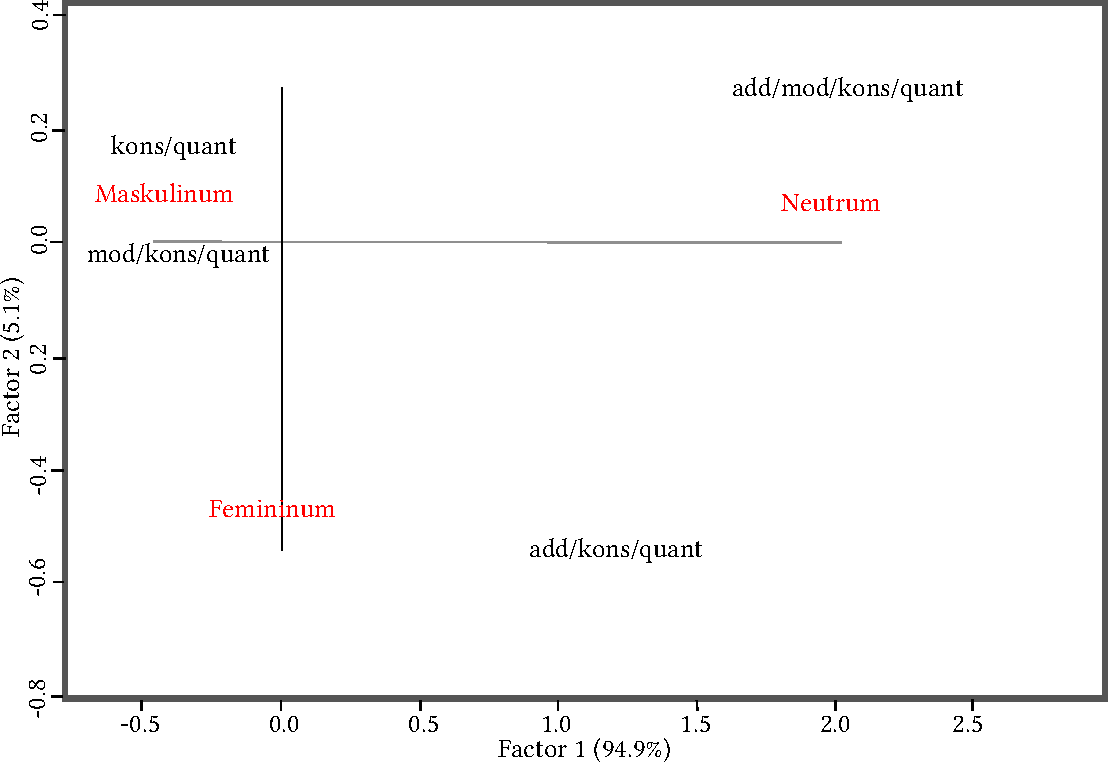
\includegraphics[width=\textwidth]{figures/revisedNickelNominalmorphologie-img024.pdf}
\caption{Korrespondenzanalyse der Variablen Genus und Pluralmarkierungsverfahren ($n=507$)}
\label{fig:7}
\end{figure}

Zusammenfassend lässt sich sagen, dass synchrone Lenis-Fortis-Alternationen (meist in Kombination mit Kontrasten der Vokalquantität) mehrheitlich durch diachronen phonologischen Wandel und damit lautgesetzlich entstanden sind. Darüber hinaus finden sich einzelne Beispiele für analoge Lenis-Fortis-Kontraste, sodass von einem funktionalisierten und zumindest teilweise produktiven Ko"-die"-rungs"-ver"-fah"-ren ausgegangen werden kann. Gleichzeitig zeigen die Daten, dass Lenis-Fortis-Kontraste nicht nur ein „Doppelleben“ \citep{Seiler2008} zwischen Phonologie und Morphologie führen, sondern dass auch Variation in der Artikulation, d.\,h. auf der phonetischen Ebene, vorhanden ist. Diese Variation besteht einerseits diachron in Form von Dialektwandel für dieses Dialektmerkmal (vgl. die vorgestellten instrumentalphonetischen Studien), und auch synchron spiegeln die BSA-Daten wider, dass Quantitätskontraste weniger binär sind, sondern innerhalb eines phonetischen Kontinuums stattfinden. Der entscheidende Punkt ist demnach weniger das Doppelleben zwischen Phonologie und Morphologie, sondern vielmehr das Doppelleben, das Lenis-Fortis-Kontraste als Kodierungsverfahren und im Sprachgebrauch der einzelnen Sprecher führen:\footnote{Vgl. hierzu \citegen[84--85]{Seiler2018} Überlegungen zu Chomskys Konzept I(nternal)- vs. E(xternal)-language.} In welchem Maße tolerieren Sprecher und Hörer des Nord- und Mittelbair. Schwankungen und eventuelle Uneindeutigkeiten der Vokal- und Konsonantenquantität, solange der Kontext die Numerusinformation disambiguiert?\footnote{Ambig sind Formen derweil nur, wenn Pluralmarkierung nur durch Lenis-Fortis-Kontraste und nicht in Form eines kombinierten Verfahrens erfolgt.}  In welchen Kontexten wird die Variation in der sprecherseitigen Realisierung vereindeutigt? Aus flexionsmorphologischer Perspektive schließt sich folgende Frage an: Wieviel Variation „verträgt“ ein Pluralmarkierungsverfahren? Anhand des untersuchten Materials (insbesondere im Hinblick auf Transkriptionseffekte) kann nicht abschließend geklärt werden, wo die Grenzen der Variation für dieses stammaffizierende Markierungsverfahren liegen. Und für die flexionsmorphologische Klassifikation stellt sich schließlich die Frage, in welchem Maße Quantitätskontraste überhaupt eine eigene Deklinationsklasse konstituieren können, wenn sie so anfällig für phonetische Variation sind (siehe \sectref{sec:8.1}).

Mit Blick auf den Sprachgebrauch ist Variation bei der Realisierung der Lenis-Fortis-Opposition einerseits auf der Produktions- und Perzeptionsebene anzusiedeln (nämlich zwischen Sprach\-ökonomie und Explizitheit der Markierung flexivischer Information, vgl. \citealt[88]{Seiler2018}, ausführlicher hierzu \sectref{sec:10.3}). Ein weiterer Aspekt von Variation kann durch das Sprachsystem lizensiert sein. \citet[124]{Steininger1994} beschreibt die Möglichkeit fakultativer Pluralmarkierung bei Lenis-Fortis-Kontrasten im Dialekt Oberneureutherwaids. Wie auch beim potenzierten Plural nach \textit{n}{}-Erweiterung im Singular der Feminina (Typ \teuthoo{das\#n}{dašn} -- \teuthoo{das\#nA}{dašnα} ‚Tasche‘) werden die Quantitätskontraste zur Disambiguierung genutzt. Ist der Plural bereits durch ein Zahlwort markiert, erfolgt keine innerparadigmatische Alternation; Leniskonsonanz ist dann auch in der Pluralform im Auslaut möglich: \textit{d̥iːʒ} -- \textit{d̥iʃ} ‚Tisch‘, aber \textit{t̥sβæ d̥i:ʒ} ‚zwei Tische‘ (\citealt[124]{Steininger1994}, vgl. \sectref{sec:9.2}). Gleichzeitig findet tatsächlich ein Wandel in der Pluralmarkierung statt, wie \citet{Wildfeuer2001} in seinem Apparent-time-Vergleich dreier Altersgruppen nachweist. Im mittelbair. Dialekt von Kirchdorf findet ein Abbau der Pluralmarkierung mittels Quantitäts- und Lenis-Fortis-Kontrast für das Lexem \textit{Tisch} statt. Ca. 70\,\% bzw. 80\,\% der Gewährspersonen der beiden älteren Sprechergruppen bilden den Plural nach diesem Muster, während in der jüngeren Sprechergruppe die Mehrzahl (60\,\%) den Plural nicht markiert (Nullplural gegenüber 40\,\% mit Kontrast der Vokalquantität und Lenis/Fortis, vgl. \citealt[189--190]{Wildfeuer2001}).

\subsubsubsection{Konsonantenelision -- 0/K- vs. K/0-Alternationen}\label{sec:7.1.2.3.2}\largerpage
Eine zweite Form der Pluralmarkierung mittels Konsonantismuskontrast besteht im gesamten UG in der innerparadigmatischen Alternation zwischen Formen mit elidiertem vs. erhaltenem Konsonanten. Die Beispiele in \tabref{tab:30} belegen verschiedene Muster der Konsonantenelision. In der Singularform ist der auslautende Plosiv oder Nasal jeweils elidiert, in allen drei Diminutivformen dagegen erhalten.\footnote{Die Diminutivformen werden hier (wo möglich) vergleichend herangezogen, da der auslautende Nasal oder Obstruent vor dem Diminutivsuffix erhalten ist. Die Berücksichtigung von Diminutiven hat aus Perspektive der Formenbildung den Vorteil, dass Diminutivbildungen ein hohes Maß an formaler Regelmäßigkeit aufweisen (vgl. \citealt[110]{Rowley1997}). Hinzu kommt mit Blick auf die Datenlage, dass sie als einziger Wortbildungstypus sehr regelmäßig und im gesamten UG in den BSA-Erhebungen abgefragt wurden.} Für die Pluralformen können nun drei Muster unterschieden werden, die als zwei unterschiedliche Wechseltypen klassifiziert werden.


\begin{table}
\begin{tabular}{llll}
\lsptoprule
{Singular} & {Plural} & {Diminutiv} & \\
\midrule
 \teuthoo{bu2E}{būə} & \teuthoo{bu2E\textbf{w}E}{būə\textbf{w}ə}
 & \teuthoo{bu"?E\textbf{w}lE}{bǖə\textbf{w}lə} & ‚Bube‘ (Gemünden am Main)\\
 \teuthoo{s\#lo24}{šlọ̄} & \teuthoo{s\#la24g}{šlạ̄\textbf{g}} & \teuthoo{s\#la24\textbf{g}Al}{šlạ̄\textbf{g}αl} & ‚Schlag‘ (Blaibach)\\
 \teuthoo{dso"+}{dsȭ} & \teuthoo{dse"+}{dsẽ̄} & \teuthoo{dsa24\textbf{n}ErlA}{dsạ̄\textbf{n}ərlα}
 & ‚Zahn‘ (Nabburg) \\
\lspbottomrule
\end{tabular}
\caption{Konsonantenelision des Wechseltypus 0/K und 0/0}
\label{tab:30}
\end{table}

\begin{sloppypar}
In Singular-/Pluralformen des Typus \teuthoo{bu2E}{būə} -- \teuthoo{bu2EwE}{būəwə} ist der Konsonant als Stammauslaut im Singular elidiert, im Plural ist er im Inlaut vor dem Pluralsuffix erhalten; die Pluralmarkierung besteht damit in einer Kombination aus additivem und stammaffizierendem Verfahren. Die Pluralmarkierung des Typus \teuthoo{s\#lo24}{šlọ̄} -- \teuthoo{s\#la24g}{šlạ̄ɡ} hingegen ist rein stammaffizierend. Der im Singular elidierte Konsonant ist im Plural erhalten, sodass die Pluralform durch Modulation der Stammvokalqualität und innerparadigmatischer Konsonantismusalternation gebildet wird. Die beiden Typen \teuthoo{bu2E}{būə} -- \teuthoo{bu2EwE}{būəwə} und \teuthoo{s\#lo24}{šlọ̄} -- \teuthoo{s\#la24g}{šlạ̄ɡ} können hinsichtlich der Konsonantismusalternation und in Anlehnung an \citet[123--125]{Rowley1997} als Wechseltypus 0/K zusammengefasst werden: \textit{0} (d.\,h. Elision) im Singular, \textit{K} (d.\,h. Konsonant) im Plural.
\end{sloppypar}

Die Singular-/Pluralform des Typus \teuthoo{dso"+}{dsȭ} -- \teuthoo{dse"+}{dsẽ̄} entspricht einem zweiten Muster, dem Wechseltypus 0/0, d.\,h. hier ist der auslautende Konsonant im Singular und im Plural elidiert und nur in der Diminutivform erhalten. Erhalt vs. Elision des stammauslautenden Konsonanten kann lexemweise in den Ortsdialekten verschieden realisiert sein, wobei sich im gesamten UG die einzelnen Typen nachweisen lassen (daneben die Variante K/K mit erhaltenem Konsonant in beiden Formen, die im Folgenden der Vollständigkeit halber aufgeführt ist, vgl. 	\tabref{tab:31} exemplarisch für das Lexem \textit{Markt}). Welcher der Wechseltypen für ein Lexem realisiert wird, unterliegt arealen, z.\,T. recht kleinräumigen Schwankungen (vgl. \citealt[124]{Rowley1997}).


\begin{table}
\begin{tabularx}{\textwidth}{lQQ}
\lsptoprule
\makecell[tl]{{Konsonan-}\\{tismus}} & {Pluralmarkierungsverfahren} & {Ortsdialekte}\\
\midrule
K/K & \textit{Vokalqualität} \textit{(Umlaut)}

Typ \teuthoo{mo:rgd5}{mo{\doubleogonek}rɡd̩} -- \teuthoo{ma4rgd}{mạrɡd} (Wolfersdorf) & bair. Wolfersdorf, Zwiesel;

ofr. Hallerstein, Mitteleschenbach, Wiesthal\\
\tablevspace
& \textit{Vokalqualität} \textit{(Umlaut)} \textit{+} \textit{e}

Typ \teuthoo{moAkt\_}{moαktʰ} -- \teuthoo{meEkte\$}{meəkte̤} (Groschlattengrün) & bair. Grafenkirchen, Groschlattengrün, Oberdolling;

ofr. Gebsattel, Gemünden am Main, Krum\\
\tablevspace
& \textit{Null}

Typ \teuthoo{margd}{marɡd} -- \teuthoo{margd}{marɡd} (Hüttenheim) & bair. Kirchensur, Ramsau bei Berchtesgaden;

ofr. Hüttenheim\\
\tablevspace
0/0 & \textit{Vokalqualität} \textit{(Umlaut)}

Typ \teuthoo{ma.kH}{maͅkhͯ} -- \teuthoo{ma4kH}{mạkhͯ} (Waldhof) & mittelbair. Waldhof\\
\tablevspace
& \textit{Null}

Typ \teuthoo{moA4k\_}{moα̣kʰ} -- \teuthoo{moA4k\_}{moα̣kʰ} (Bernried) & bair. Bernried, Inning am Holz, Windischeschenbach;

ofr. Kirchensittenbach\\
\tablevspace
0/K & \textit{Vokalqualität} \textit{(Umlaut)}

Typ \teuthoo{A}{α} \teuthoo{mo.Ak,\_}{moͅαk͓ʰ} -- \teuthoo{ma4k,t,}{mạk͓t͓} (Bernhardswald) & bair. Bernhardswald, Kallmünz;

ofr. Pfofeld, Stadtschwarzach, Wilhermsdorf\\
\tablevspace
& \textit{Vokalqualität} \textit{(Umlaut)} \textit{+} \textit{e}

Typ \teuthoo{ma.rk}{maͅrk} -- \teuthoo{me.<rk,te4}{mêͅrk͓tẹ} (Niedertaufkirchen) & mittelbair. Niedertaufkirchen, Pasing, Reischach\\
\tablevspace
K/0 & \textit{Vokalqualität} \textit{(Umlaut)}

Typ \teuthoo{moAkt}{moαkt} -- \teuthoo{meEk}{meək} (Nabburg) & nordbair. Nabburg\\
\lspbottomrule
\end{tabularx}
\caption{Varianten der Konsonantismusalternation im UG für \textit{Markt}}
\label{tab:31}
\end{table}

\begin{sloppypar}
In \tabref{tab:31} ist ein vierter Wechseltypus (K/0) aufgeführt, bei dem der auslautende Konsonant in der Singularform erhalten, in der Pluralform hingegen elidiert ist. Die Struktur von Singular- und Pluralform dieses Wechseltypus gleicht einem subtraktiven Pluralmarkierungsverfahren: Der Stamm der Pluralform wird im Auslaut um ein Phonem reduziert (vgl. \citealt[582f.]{Dressler2000}, \citealt[25]{Birkenes2014} sowie \sectref{sec:7.1.2.4}). Die phonologischen Prozesse hinter dem K/0-Alternationsmuster sind sprachhistorisch jedoch von subtraktiver Morphologie zu unterscheiden, wie die folgenden Darstellungen zeigen werden.
\end{sloppypar}

Die Belege weiterer K/0-Alternationen in \tabref{tab:32} illustrieren, dass es sich im gesamten Korpus um ein eher peripheres Phänomen handelt, das ein Spezifikum des Bair., und zwar des Nordbair. zu sein scheint. Für die in 	\tabref{tab:32} aufgeführten Lexeme lassen sich im gesamten UG auch die übrigen Wechseltypen nachweisen. Die übergeordnete Frage lautet daher: Wie lassen sich die verschiedenen Fälle von innerparadigmatischer Alternation aus flexionsmorphologischer Perspektive systematisieren und modellieren? Stellt die innerparadigmatische Konsonantismusalternation durch Elision bzw. Erhalt des stammauslautenden Konsonanten ein eigenes Pluralmarkierungsverfahren dar (und inwiefern ist es als solches kognitiv verankert und überhaupt produktiv), inwiefern ist die innerparadigmatische Konsonantismusalternation aber auch nur eine phonetisch-phonologische „Begleiterscheinung“ der Pluralbildung?

\begin{table}[H]
\begin{tabular}{llll}
\lsptoprule
{Singular} & {Plural} & {Diminutiv} & \\
\midrule
\teuthoo{moAk\textbf{t}}{moαk\textbf{t}} & \teuthoo{meEk}{meək} &  & ‚Markt‘ (nordbair. Nabburg)\\
\teuthoo{ro2\textbf{d}}{rōi\textbf{d}} & \teuthoo{re42}{rẹ̄} & \teuthoo{ra42\textbf{d}l@}{rạ̄\textbf{d}l} & ‚Rad‘ (nordbair. Nabburg) \\
\teuthoo{lo<A\textbf{b}}{lôα\textbf{b}} & \teuthoo{lo2i}{lōi}. &  & ‚Laib‘ (nordbair. Windischeschenbach) \\
\teuthoo{mo2A\textbf{d}}{mōα\textbf{d}} & \teuthoo{mo9.2i}{mo\klammeruntenpost{}̄ͅi} &  & ‚Magd‘ (nordbair. Nabburg) \\
\teuthoo{tSa4o\$(+\textbf{n}}{tʃạõ\textbf{n}} & \teuthoo{t,S,ôo+i:6}{t͓ʃ{\aufstrih}õi{\doubleogonek}̃} &  & ‚Zaun‘ (mittelbair. Inning am Holz)\\
\lspbottomrule
\end{tabular}
\caption{Konsonantenelision des Wechseltypus K/0}
\label{tab:32}
\end{table}

Die Anzahl der Lexeme, die im Flexionsparadigma zwischen elidiertem vs. erhaltenem Konsonanten alternieren, ist im Korpus begrenzt und aufgrund der schwankenden regionalen Geltung „letztendlich Aufgabe der Ortsgrammatiken“ \citep[124]{Rowley1997}. Insgesamt handelt es sich um ein nicht allzu typenfrequentes Phänomen, das vor allem im Bair. zu einer spezifischen Formenbildung geführt hat. Da die Elision in- oder auslautender Obstruenten und Nasale auf unterschiedliche Regelmäßigkeiten und historische Entwicklungen zurückgeht, werden sie im Folgenden getrennt dargestellt.

\subsubsubsubsection{Elision von Obstruenten in Vokal-Konsonant-Abfolgen}

Der Schwund des Obstruenten in Vokal-Konsonant-Abfolgen und in der Finalposition in Konsonantenclustern ist diachron durch unterschiedliche phonologische Prozesse (Tilgung oder Assimilation an den vorausgehenden Konsonanten) entstanden. Da die innerparadigmatische Alternation zwischen erhaltenem vs. geschwundenem Konsonanten oder in Konsonantenclustern aus flexionsmorphologischer (und damit synchroner) Perspektive demselben Pluralmarker entspricht, werden die Phänomene im Folgenden gemeinsam behandelt.


\begin{map}
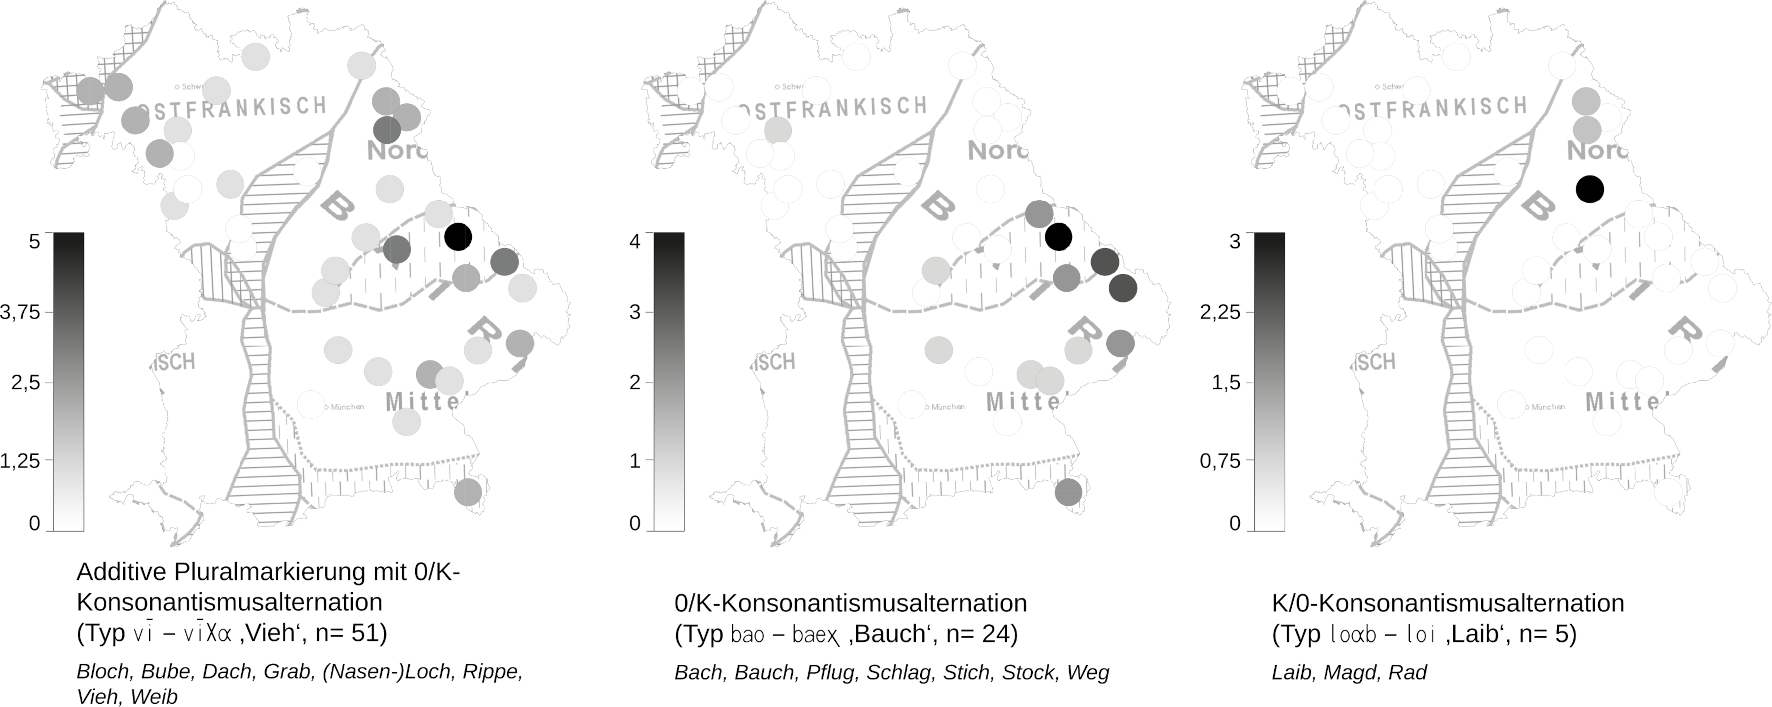
\includegraphics[width=\textwidth]{figures/Karte15.png}
\caption{Absolute Häufigkeit pro Ortsdialekt von innerparadigmatischer Alternation durch Konsonantenelision bei Vokal-Obstruent-Abfolge ($n=80$)}
\label{map:15}
\end{map}

\mapref{map:15} fasst die absolute Häufigkeit innerparadigmatischer Konsonantenelisionen im absoluten Auslaut bei Vokal-Obstruent-Abfolgen zusammen. Die Alternationen sind bei den einzelnen Lexemtypes im Korpus jeweils nur mit geringer Tokenanzahl belegt, insgesamt liegt eine z.\,T. recht kleinteilige, lexemspezifische areale Geltung vor. In Abhängigkeit von der konkreten Pluralmarkierungsstrategie können jedoch zwei Typen innerparadigmatischer Alternationen beschrieben werden: Wechsel zwischen elidiertem und erhaltenem Konsonanten (bzw. Konsonantenabfolge) in additiven Pluralformen (Typ \teuthoo{vi“}{vī} -- \teuthoo{vi“cA}{vīXα} ‚Vieh‘) und Wechsel zwischen elidiertem und erhaltenem Konsonanten in stammaffizierenden Pluralformen (Typ \teuthoo{bao}{bao} -- \teuthoo{baeX}{baeꭗ} ‚Bauch‘). Während Typ \teuthoo{vi“}{vī} -- \teuthoo{vi“cA}{vīXα} lexemweise im gesamten UG zu finden ist, stellen 0/K-Alternationen des Typs \teuthoo{bao}{bao} -- \teuthoo{baeX}{baeꭗ} ein -- wenn auch schwach besetztes -- spezifisch bair. Flexionsmuster dar.

Die Alternationen des Typs \teuthoo{bao}{bao} -- \teuthoo{baeX}{baeꭗ} sind das Ergebnis historischer phonologischer Prozesse, die Fortes und Lenes im In- und Auslaut im UG unterschiedlich affizierten.\footnote{Vgl. \citet[81--88]{Franke1895} zu einem Vergleich von Konsonantenelisionen im Ofr. und Obersächsischen (leider ohne Berücksichtigung der innerparadigmatischen Perspektive und möglicher Alternationen).} Im Zuge der sogenannten mittelbair. Konsonantenschwächung wurden die Fortisobstruenten ab ca. 1300 im Nord- und Mittelbair. lenisiert und sind z.\,T. mit den alten Lenes zusammengefallen.\footnote{Vgl. \citet[§34a und Karte 21]{Kranzmayer1956}, \citet[78--79]{Rowley1997}, \citet[271 und 302]{Schirmunski1962}.} Der bair. Dialektraum lässt sich infolge dieser Entwicklung in einen nord- und mittelbair. Teil gegenüber einem südbair. Teil mit erhaltenen Fortisobstruenten untergliedern, weshalb \citet[§34a2]{Kranzmayer1956} die Bedeutung der mittelbair. Konsonantenschwächung für das Bair. als „ebenso schwer“ wie die der hochdeutschen Lautverschiebung einordnet. Neben der nord- und mittelbair. Ausprägung des Lenisierungsprozesses greift im ofr. Teil des UGs die sogenannte binnenhochdeutsche Konsonantenschwächung, die sich z.\,T. auf das westliche Nordbair. ausdehnt (\tabref{tab:33}, vgl. \citealt[§34c1]{Kranzmayer1956}, \citealt[78]{Rowley1997}).

Aufgrund der phonologischen Prozesse Einsilberdehnung und mittelbair. Konsonantenschwächung (d.\,h. Lenisierung) bei gleichzeitig wirkendem bair. Silbengesetz kann für Einsilber mit historischem Fortisauslaut im Nord- und Mittelbair. von Leniskonsonanz im Auslaut ausgegangen werden (vgl. \citealt[28]{Grundler1951}). Hinzu kommt, dass in den Dialekten des UGs die Auslautverhärtung als Folge von Apokopierung und innerparadigmatischem Ausgleich im Singularparadigma früh zurückgenommen wurde, weshalb es, so \citet[78]{Rowley1997}, „zweckmäßig“ ist, auch bei Lexemen mit historischer Leniskonsonanz im Auslaut mhd. restituierte Lenes anzunehmen (vgl. \citealt[§27d]{Kranzmayer1956}).\largerpage[1.5]

Vor dem Hintergrund dieser historischen phonologischen Prozesse erklären sich nun die innerparadigmatischen Konsonantismusalternationen zwischen elidiertem vs. erhaltenem Obstruenten. Im primären und sekundären (d.\,h. durch Apokope entstandenen) Auslaut schwinden im Nordbair. um Cham und Teilen des Mittelbair. die mhd. restituierten Lenes \textit{b}, \textit{g}, teilweise \textit{d} sowie \textit{ch} in Einsilbern (\citealt[78]{Rowley1997}, \citealt[§28b2, 29c, 30b3, 33c]{Kranzmayer1956}). Dass rezente Konsonantismusalternationen bei Obstruenten im Kontext dieser historischen Prozesse und innerhalb des phonologischen Systems der nord- und mittelbair. Dialekte verstanden werden müssen, illustriert \citegen{Zehetner1978} Modellierung der Phoneme /b d g/ auf einem Spektrum phonetischer Realisierungen (\tabref{tab:34}).\pagebreak

\begin{table}[p]
\small
\begin{tabularx}{\textwidth}{>{\raggedright\arraybackslash}p{.17\textwidth}QQQ}
\lsptoprule
& Anlaut & Inlaut & Auslaut\\
\midrule
\multirow[2]{2}{=}{Binnen\-hoch\-deu\-tsche Kon\-so\-nan\-ten\-schwä\-chung} & \multicolumn{3}{>{\raggedright\arraybackslash}p{.8\textwidth}}{Aufhebung der Fortis-Lenis-Opposition bei mhd. \textit{p}/\textit{pp} und mhd. \textit{b}, mhd. \textit{t}/\textit{tt} und mhd. \textit{d}}\\
\tablevspace
& Erhalt von mhd. \textit{k} (außer vor \textit{l}, \textit{n}, \textit{r}) & \multicolumn{2}{>{\raggedright\arraybackslash}p{.5\textwidth}}{nicht vollständiger Zusammenfall von Fortes und Lenes aufgrund von Spirantisierung und Elision der Lenes (\citealt[78]{Rowley1997}, vgl. \citealt[34c6]{Kranzmayer1956})}\\
\tablevspace
Mittelbair. Konsonantenschwächung & Zusammenfall von mhd. \textit{p} und \textit{b}, \textit{t} und \textit{d} \citep[78]{Rowley1997}, & \multirow[t]{2}{=}{Zusammenfall von Fortes und Lenes, Lenisierung der Fortes (mit Ausnahme frühahd. Geminaten und einzelner Fortes\-konsonantenfolgen, vgl. \citealt[§34c4]{Kranzmayer1956} und \citealt[78]{Rowley1997})} & \\
\tablevspace
& \multirow[t]{10}{=}{Lenisierung der Fortes zu Halbfortes oder Halblenes (\citealt[§34c3]{Kranzmayer1956}),} &  & \\
\\
\\
\\
\\
\\
\\
\\
%\tablevspace
&  & Realisierung frühahd. Geminaten als Fortes (\citealt[§34c2]{Kranzmayer1956}) & \\
\tablevspace
&  & \multicolumn{2}{>{\raggedright\arraybackslash}p{.5\textwidth}}{Geltung des bair. Silbengesetzes: Langvokal+Lenisobstruent, Kurzvokal+Fortisobstruent -- Lenisierung von Fortes nach Langvokal (vgl. \sectref{sec:7.1.2.3.1}, \citealt[§34a, i, k]{Kranzmayer1956}, \citealt[78]{Rowley1997})}\\
\lspbottomrule
\end{tabularx}
\caption{Übersicht der Lenisierungsprozesse im UG}
\label{tab:33}
\end{table}


\begin{table}
\small
\begin{tabularx}{\textwidth}{lQQQQQQQQ}
\lsptoprule
& Af\-fri\-ka\-te & as\-pi\-rier\-te Fortes & Fortes & Halb\-fortes & Lenes & re\-du\-zier\-te Lenes & Spi\-ran\-ten & Eli\-sion\\
\midrule
Phon & [pf] & [p\textsuperscript{h}] & [p] & [\teuthoo{ç}{ç}] & [b] & [\textsuperscript{b}] & [\teuthoo{B}{{\btilde}} \teuthoo{w}{w}] & ø\\
 & [ts] & [t\textsuperscript{h}] & [t] & [\textsuperscript{d}\textsubscript{t}] & [d] & [\textsuperscript{d}] &  & ø\\
 & *[kx] & [k\textsuperscript{h}] & [k] & [\textsuperscript{k}\textsubscript{g}] & [g] & [\textsuperscript{g}] & [\teuthoo{c}{X} h] & ø\\
 \tablevspace
 \cmidrule(lr){3-7}
Phonem & /bf/ & \multicolumn{5}{c}{/b/} & {/w/} & \\
 & /ds/ & \multicolumn{5}{c}{/d/} &  & \\
 & /gh/ & \multicolumn{5}{c}{/g/} & {/h/} & \\
\lspbottomrule
\end{tabularx}
\caption{Inventar der Obstruentenphoneme und phonetische Entsprechungen im Mittelbair. der Hallertau (nach \citealt[178--179]{Zehetner1978})}
\label{tab:34}
\end{table}

Für die Vokal-Konsonant-Abfolge /Vx/ ist eine innerparadigmatische Alternation im Ofr. nur für \textit{Vieh} teilweise belegt (z.\,B. \teuthoo{v5i“}{v̩ī} -- \teuthoo{v5i“cE}{v̩īXə}, ofr. Krum), in den übrigen Tiefenbohrungspunkten wird die Singularform hier mit Frikativ im Auslaut realisiert, z.\,B. \teuthoo{vôe.ic}{v{\aufstrih}eͅiX} -- \teuthoo{vôe.icA}{v{\aufstrih}eͅiXα} (nordbair. Nabburg). Weitere Belege einer innerparadigmatischen Alternation bei /Vx/-Abfolge in mehrheitlich rein stammaffizierenden Pluralformen finden sich nur in den Tiefenbohrungspunkten des Bayerischen Waldes, im östlichen Mittelbair. sowie im mittelbair.-südbair. Ortspunkt Ramsau. Die Elision des Auslauts der Singularform ist hier Ergebnis der mittelbair. Konsonantenschwächung, z.\,B. \teuthoo{bo.2}{bōͅ} -- \teuthoo{ba4x}{bạx} --Dim. \teuthoo{ba4xl}{bạxl} ‚Bach‘ im nordbair.-mittelbair. Zwiesel (vgl. \citealt[§34k4]{Kranzmayer1956}, vgl. \citealt[§125]{Micko1930}).\footnote{Daneben findet sich in den von \citet[§33d1]{Kranzmayer1956} ausgewiesenen Gebieten des Bair. auch für die mhd. Konsonantenfolge -\textit{ht} die historische Form mit elidiertem Frikativ in der Singularform (mit Einsilberdehnung im Singular und Kurzvokal im Plural) bei \textit{Nacht} (etwa \teuthoo{dno2Ad}{dnōαd} -- \teuthoo{na\$x,d}{na̤x͓d} im nordbair. Windischeschenbach), \textrm{\textit{Knecht}} (z.\,B. \teuthoo{gNe2d}{ɡŋēd}-- \teuthoo{gNe4Xd5}{ɡŋẹꭗd̩}, nordbair.-mittelbair. Bernried) sowie teilweise bei \textit{Furche} mit auslautendem Dentalplosiv (\teuthoo{vu.Ed}{vuͅəd} -- \teuthoo{vu.Exdn@}{vuͅəxdn̥} im \textrm{nordbair}. Kallmünz\textrm{) und} \textrm{\textit{Magd}} \textrm{mit spirantisiertem /g/: \teuthoo{me.2d}{mēͅd}} -- \textrm{\teuthoo{me.xd}{meͅxd} (neben \teuthoo{me.2dn}{mēͅdn}) im ofr. Stadtschwarzach (vgl. \sectref{sec:7.1.2.3.3})}.}

In /Vg/-Abfolgen (Typ \teuthoo{s\#lo24}{šlọ̄} -- \teuthoo{s\#la4g}{šlạɡ} ‚Schlag‘) ist nach \citet[§28c1]{Kranzmayer1956} auslautendes /g/ in einem größeren Gebiet geschwunden als inlautendes /g/, u.\,a. im nordwestlichen Oberbayern und im nördlichen Bayerischen Wald, d.\,h. in jenem Areal, für das auch in den vorliegenden Daten innerparadigmatische Alternationen bei stammaffizierenden Pluralformen belegt sind. Bei der Vo\-kal-""Kon\-so\-nant-""Ab\-fol\-ge /Vb/ ist /b/ im primären und sekundären Auslaut im Nord- und Mittelbair. weitgehend getilgt (\citealt[§30b3]{Kranzmayer1956}, vgl. \citealt[305]{Schirmunski1962}). Auch \citet[35--36]{Lessiak1933} führt für das Bair. und Ofr. völligen Schwund von germ. \textit{b} an, der teilweise nur im sekundären Auslaut erfolgte (vgl. \citealt[Karte 9]{Roth1940}, \citealt[219]{Steger1968}).


\begin{table}
\small
\begin{tabularx}{\textwidth}{lllllQ}
\lsptoprule
& {Nom.Sg.} & {Nom.Pl.} & {Diminutiv} & {Dat.Pl.} & \\
\midrule
(1) & \teuthoo{bu.2E}{būͅə} & \teuthoo{bu.2E.vE}{būͅəͅvə} & \teuthoo{b{\textasciitilde}îi.“Ervl.E}{b{\aufstrih}īͅərvlͅə} & \teuthoo{mi.d}{miͅd} \teuthoo{bu9.2E.vE}{bu\klammeruntenpost{}̄ͅəͅvə} & ofr. Gebsattel\\
(2) & \teuthoo{bu942A}{bu\klammeruntenpost{}̣̄α} & \teuthoo{bu9.2m}{bu\klammeruntenpost{}̄ͅm} & \teuthoo{bi.“b,l.9A94}{bīͅb͓lͅ\klammeruntenpost{}α\klammeruntenpost{}̣} & \teuthoo{ge.2An}{ɡēͅαn} \teuthoo{mi.d}{miͅd}i. \teuthoo{bu9.2m}{bu\klammeruntenpost{}̄ͅm} & ofr. Burgbernheim \\
(3) & \teuthoo{bôo<u.}{b{\aufstrih}ôuͅ} & \teuthoo{bôo<u.m}{b{\aufstrih}ôuͅm} & \teuthoo{bôo<(u.Bedý@}{b{\aufstrih}ô\klammerobenpost{}uͅ{\btilde}edɫ̥} & \teuthoo{min}{min} \teuthoo{b5ôo>?(?u.BAn}{b̩{\aufstrih}ö̂̈\klammerobenpost{}uͅ{\btilde}αn} & nordbair. Windischeschenbach\\
(4) & \teuthoo{bo:u}{bo{\doubleogonek}u} & \teuthoo{bo:umA}{bo{\doubleogonek}umα} & \teuthoo{be.iwAl}{beͅiwαl} & \teuthoo{midn@}{midn̥} \teuthoo{bo:umAn}{bo{\doubleogonek}umαn} & nordbair.-mittelbair. Blaibach\\
\lspbottomrule
\end{tabularx}
\caption{Flexions- und Diminutivformen für \textit{Bube}}
\label{tab:35}
\end{table}

Die Zusammenschau der Belege zeigt, dass innerparadigmatische Alternationen bei /Vb/ in additiven Pluralformen insbesondere im Bair. vorkommen und da lexemweise auch großräumig gelten (etwa bei \textit{Grab} und \textit{Weib}). Die Realisierung des /b/ ist dabei von der Form des Pluralsuffixes abhängig ist: /b/ (bzw. eine spirantisierte Variante) erscheint regelmäßig nur bei vokalischem Suffix -\textit{ə} oder -\textit{α}, z.\,B. \teuthoo{wâa<e\$<}{w{\aufstrih}âê̤} -- \teuthoo{twâa4<e\$+wA}{tw{\aufstrih}ậẽ̤wα} ‚Weib‘ im mittelbair. Inning am Holz oder \teuthoo{gro942}{ɡro\klammeruntenpost{}̣̄} -- \teuthoo{gra42BA}{ɡrạ̄{\btilde}α} ‚Grab‘ im nordbair. Groschlattengrün. Während das auslautende /b/ im Primärauslaut in \textit{Weib} und \textit{Grab} in den übrigen Dialekten des UGs erhalten ist, ist dessen Schwund für das Lexem \textit{Bub} in den bair. Dialekt „allgemein“ (\citealt[§30b3]{Kranzmayer1956}), in den vorliegenden Daten als innerparadigmatische Alternation zwischen Singular- und Pluralform aber nur für das westliche Ofr. belegt (vgl. \citealt[§51]{Frommann1857}). In diesen Ortsdialekten, die alle im sogenannten Vokalisierungsstreifen liegen, wird der Plural durch ein vokalisches Schwa-Suffix markiert (Beispiel (1) in 	\tabref{tab:35}). In den übrigen Tiefenbohrungspunkten im Ofr., Nord- und Mittelbair. wird der Plural ebenfalls additiv gebildet, das Nasalsuffix ist hier an das stammauslautende /b/ assimiliert (Beispiele (2) und (3), vgl. die jeweiligen Diminutivformen). Für die Orte Blaibach (Beispiel (4)) und Bernhardswald (\teuthoo{bôo.u}{b{\aufstrih}oͅu} -- \teuthoo{bôo.umA}{b{\aufstrih}oͅumα}) im nordbair.-mittelbair. Übergangsgebiet sind Pluralformen mit Doppelsuffigierung belegt: An das assimilierte Nasalsuffix ist ein weiteres \teuthoo{A}{α}{}-Suffix getreten. Interessant sind außerdem die Dativ-Pluralformen, die für \textit{Bube} abgefragt wurden (ausführlicher \sectref{sec:7.2.1}).\footnote{Abgefragt wurde der Satzkontext „\textit{Die kleinen Mädchen spielen gern mit anderen Mädchen, aber sie spielen nicht gerne} mit den Buben“.}


\begin{map}
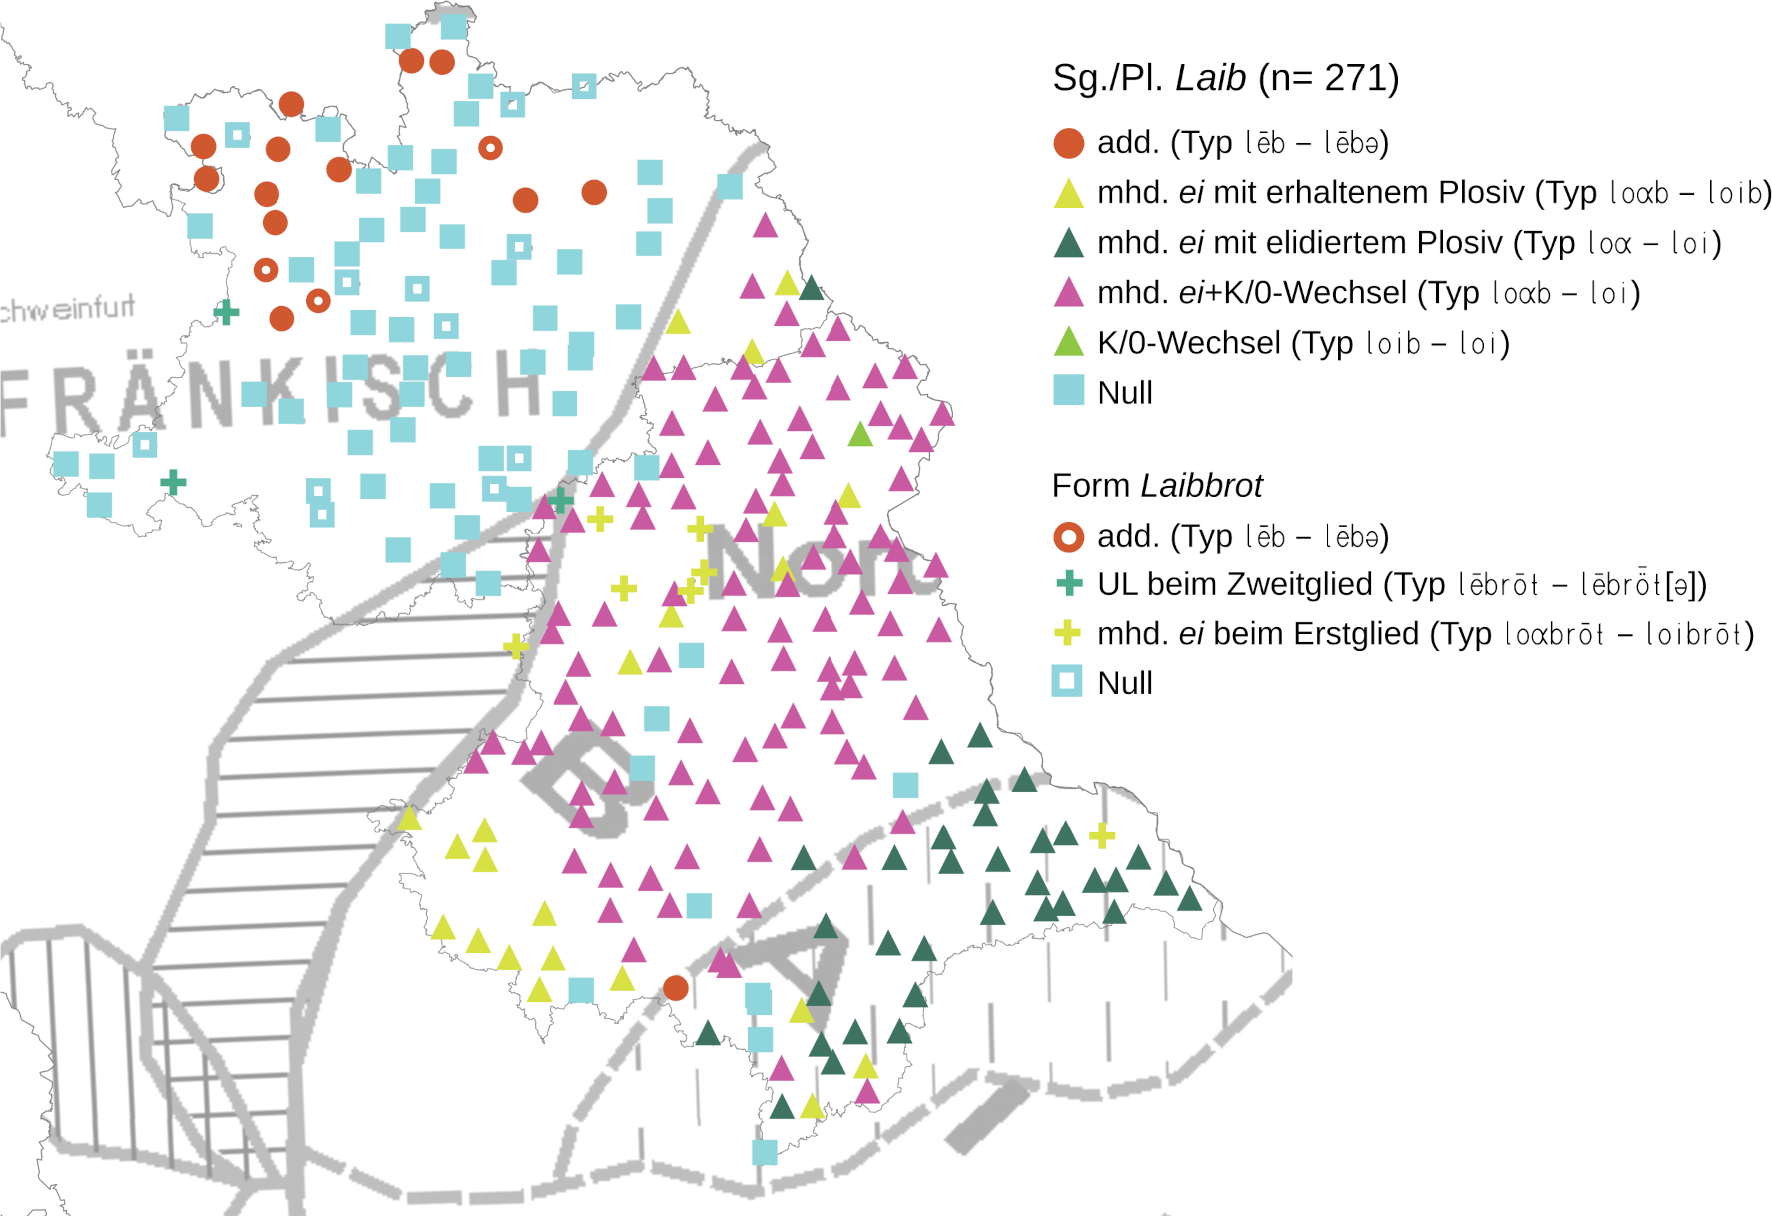
\includegraphics[width=\textwidth]{figures/Karte16.png}
\caption{Pluralmarkierung bei \textit{Laib} im SNOB}
\label{map:16}
\end{map}

Neben den 0/K-Alternationen in stammaffizierenden und additiven Pluralformen wurde in \mapref{map:15} auch die absolute Vorkommenshäufigkeit von K/0-""Al\-ter\-na\-tio\-nen dargestellt. Es zeigt sich, dass Alternationen des Typs \teuthoo{loAb}{loαb} -- \teuthoo{loi}{loi} ‚Laib‘ nur im mittleren und nördlichen Nordbair. vorkommen. In der Literatur werden für die K/0-Alternation im Nordbair. nur vereinzelte Belege angeführt (z.\,B. zum nordbair. Eslarn \citealt[86]{Bachmann2000}, für das Egerländische \citealt[122]{Roth1940}). Um die tatsächliche areale Verbreitung und areale Geltung dieser Form der Konsonantismusalternation zu ermitteln, habe ich sämtliche Rohdaten der entsprechenden Fragen zu Sg./Pl. \textit{Laib} für das nordostbayerische SNOB-Gebiet ausgewertet (\mapref{map:16}).\footnote{\textrm{Für 181 Untersuchungsorte des SNOB-Teilprojekts konnten keine Singular- und Pluralformen ausgewertet werden, da die Transkripte (noch) nicht in der} \textrm{\textit{BayDat}} \textrm{hinterlegt sind oder die Formen nicht abgefragt wurden. Zudem konnte ein Teil der Antworten der Gewährspersonen nicht berücksichtigt werden, da die Gewährspersonen ein Heteronym verwendet haben oder die Segmentierung der Transkripte nicht eindeutig war: Im Fragebuch wurde neben dem Simplex} \textrm{\textit{Laib}} \textrm{auch} \textrm{\textit{Laib Brot}} \textrm{und das Kompositum} \textrm{\textit{Laibbrot}} \textrm{suggeriert, das im SNOB-UG teilweise üblich ist. Wurde die Form} \textrm{\textit{Laibbrot}}\textrm{/}\textrm{\textit{Laib Brot}} \textrm{in nur einer der Formen realisiert, konnte der Beleg in der Regel nicht ausgewertet werden, da die Klassifikation der Realisierung des auslautenden Plosivs einzig anhand der} \textrm{\textit{BayDat}}\textrm{{}-Kodate nicht unsicher ist.}} Die Variantenverteilung in \mapref{map:16} illustriert, dass die K/0-Alternation für die Singular- und Pluralform von \textit{Laib} des Typs \teuthoo{loAb}{loαb} -- \teuthoo{loi}{loi} ein spezifisch nordbair. Phänomen. ist. Im gesamten nordbair. Teil des UG findet sich der umlautähnliche Diphthongwechsel von mhd. \textit{ei} (vgl. \sectref{sec:7.1.2.1.2}). Im nordbair.-mittelbair. Übergangsgebiet ist /b/ im primären und sekundären Auslaut entfallen (Typ \teuthoo{loA}{loα} -- \teuthoo{loi}{loi}), im Südwesten der Oberpfalz und vereinzelt im nördlichen Nordbair. ist /b/ im primären und sekundären Auslaut erhalten (Typ \teuthoo{loAb}{loαb} -- \teuthoo{loib}{loib}). Im Norden des ofr. Teils des UG wird der Plural von \textit{Laib} additiv gebildet, im übrigen Gebiet des Ofr. findet sich Nullplural (vereinzelt auch im Nordbair.).

Zwei weitere Belege für K/0-Wechsel im Nordbair. finden sich in den vorliegenden Daten für die Vokal-Konsonantenfolge /Vd/: \teuthoo{mo2Ad}{mōαd} -- \teuthoo{mo9.2i}{mo\klammeruntenpost{}̄ͅi} ‚Magd‘ und die suggerierte Form \teuthoo{ro2d}{rōd} -- \teuthoo{re42}{rẹ̄} ‚Rad‘ (neben \teuthoo{ra42dl@}{rạ̄dl̥} -- \teuthoo{ra42dl@n}{rạ̄dl̥n}) im nordbair. Nabburg. Die Pluralform für \textit{Magd} wird wie auch bei \textit{Laib} im nordbair. UG durch stammaffizierende Markierung gebildet, weshalb eine weitere Kartierung des gesamten SNOB-Materials als Vergleichskarte sinnvoll erschien.\footnote{Für das Neutrum \textit{Rad} finden sich vor allem Pluralformen des Typs \textit{Rad} -- \textit{Räder}. Eine erste Durchsicht der SNOB-Rohdaten in \textit{BayDat} hat allerdings eine weitere Form für ofr. Blankenberg (Thüringen) ergeben: \teuthoo{ro.ûud}{rỗ̃ͅ{\aufstrih}ud} -- \teuthoo{re:2}{re{\doubleogonek}̄} ‚Rad‘.} \mapref{map:17} zeigt, dass sich die Variante \teuthoo{moAd}{moαd} -- \teuthoo{moi}{moi} mit K/0-Alternation in einem ähnlichen, aber kleineren Areal findet wie bei \textit{Laib}. Im Nordosten des Nordbair. ist die Varianten mit erhaltenem Plosiv im primären und sekundären Auslaut belegt (Typ \teuthoo{moAd}{moαd} -- \teuthoo{moid}{moid}).\footnote{Vgl. \citet[124]{Roth1940} zur Konsonanten-Alternation K/0 im Egerländischen: „Die Form \textit{mei} ist nur im Ascher Land und in der nordöstlichen Übergangszone erhalten, sonst herrscht \textit{mēid}.“}

\begin{map}
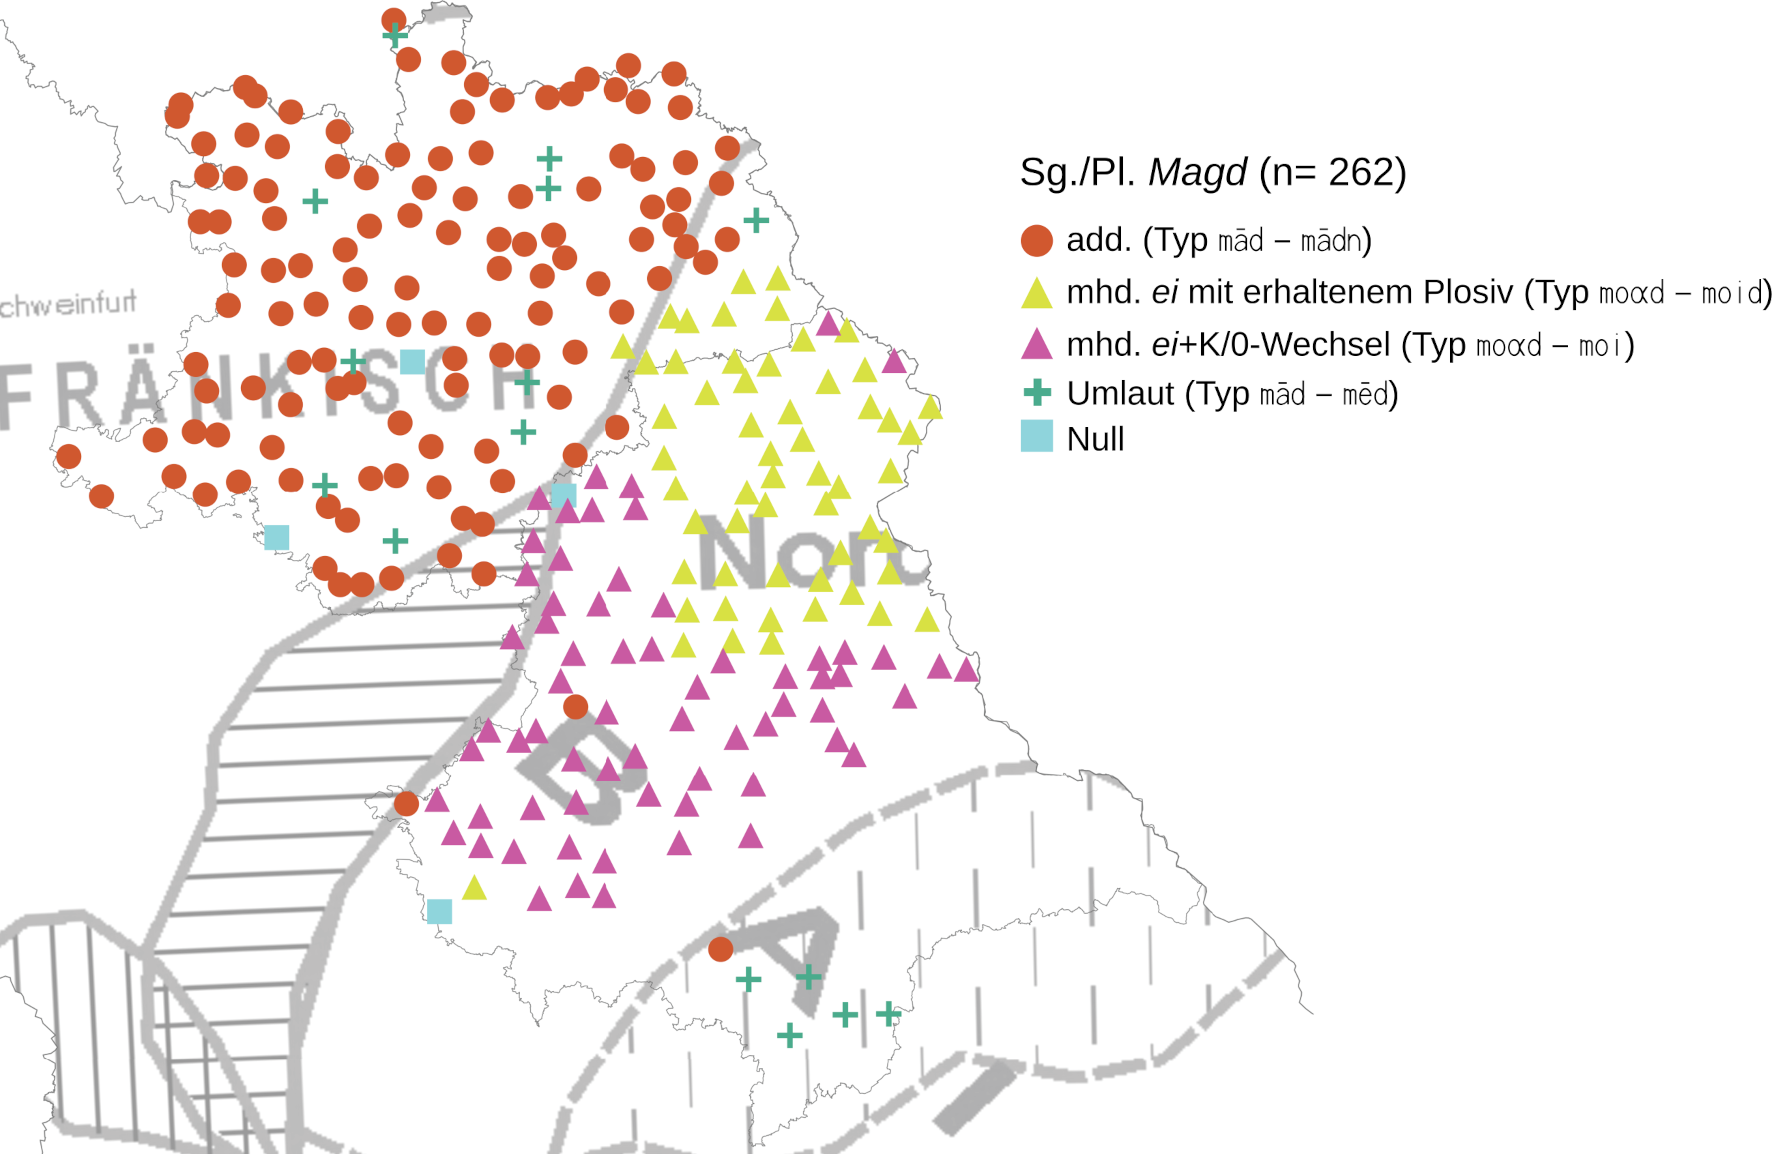
\includegraphics[width=\textwidth]{figures/Karte17.png}
\caption{Pluralmarkierung bei \textit{Magd} im SNOB\protect\footnote{Das Heteronym \textit{Dirn} im Süden des UGs wurde nicht kartiert.}}
\label{map:17}
\end{map}

Wie auch bei subtraktiver Morphologie im phonologischen Kontext von Vokal-Konsonant-Abfolgen sind die dargestellten innerparadigmatischen Konsonantismusalternationen das Ergebnis von Lenisierungen (vgl. \citealt[82]{Birkenes2014}). Anders als bei \citeauthor{Birkenes2014}' (\citeyear{Birkenes2014}) subtraktiven Flexionsformen ist Lenisierung im Bair. nicht nur in intervokalischer Umgebung, sondern auch im absoluten Auslaut wirksam; in unterschiedlichen phonologischen Umgebungen tritt sie im primären und im sekundären Auslaut ein. Bei Singular-/Pluralformen des 0/K-Typs ist der Konsonant im absoluten Auslaut der Singularform elidiert, in der (ehemals) intervokalischen Position der Pluralform aber erhalten (bzw. beim 0/0-Typ auch in dieser Position elidiert). In Teilen des Nordbair. ist -- lexemweise -- der auslautende Plosiv im primären Auslaut der Singularform erhalten, aber im sekundären Auslaut der Pluralform getilgt, weshalb die Formen mit K/0"=Konsonantenalternation in diesem Gebiet zu finden sind. Inwiefern diese Formen der Pluralmarkierung produktiv sind oder ob es sich um Relikte der phonologischen Prozesse der mittelbair. Konsonantenschwächung handelt, kann mit den vorliegenden Daten nicht beantwortet werden; zumindest konnten sie nicht außerhalb der bekannten phonologischen Kontexte nachgewiesen werden. Es scheint sich also um lexikalisierte morphophonologische Alternationen zu handeln. Während die 0/K"=Alternationen im Nord- und Mittelbair. als „längere“ Pluralformen mit erhaltenem Konsonanten dem Prinzip „Mehr Inhalt, mehr Form“ entsprechen, laufen K/0"=Alternationen -- wie subtraktive Pluralformen auch -- diesem Prinzip entgegen: Semantisches Mehr wird hier durch weniger Form kodiert.

\subsubsubsubsection{Elision des finalen Plosivs in Konsonantenclustern}\largerpage[-1]

Beide Muster der innerparadigmatischen Konsonantismusalternation (0/K, K/0) finden sich auch für die finalen Plosive in Konsonantenclustern, sie sind hier das Ergebnis von Konsonantenassimilation. Zwar können an dieser Stelle nur Tendenzen aufgezeigt und exemplarische Fälle diskutiert werden, da -- wie \mapref{map:18} illustriert -- in den BSA-Erhebungen für die einzelnen Konsonantencluster nur wenige Items abgefragt wurden. Gleichzeitig geben diese exemplarischen Fälle Einblicke in die spezifisch dialektale Formenbildung und eröffnen grundsätzlichere Fragen der Flexionsmorphologie, wie weiter unten gezeigt wird.

Für die einzelnen Lexeme mit finalem Konsonantencluster haben Konsonantismusalternationen im UG zum Teil großräumige, teilweise aber auch recht kleinräumige regionale Geltung. Innerparadigmatische Alternationen bei additiven Pluralformen finden sich für das Konsonantencluster /ld/ im Neutrum \textit{Feld} (K/0"=Alternation \teuthoo{vôe"?l.d.}{v{\aufstrih}ë̄lͅdͅ} -- \teuthoo{vôe.l.A}{v{\aufstrih}eͅlͅα} neben 0/K"=Alternation \teuthoo{ve.2i“.}{vēͅīͅ} -- \teuthoo{ve.2i“dA).}{vēͅīdα\klammeruntenpost{}ͅ}\footnote{Im Ofr. erfolgt für die /ld/-Abfolge teilweise die Assimilation des Dentalplosivs in intervokalischer Position, \citet[§28c]{Kranzmayer1956} nennt die assimilierten Formen daneben für das Nord- und Mittelbair. (mit Ausnahme weiter Teile Ober- und Niederbayerns, vgl. \citealt[400]{Schirmunski1962}, vgl. \citealt{WA}-Karte 524 „Felde“). Auch \citet[69f.]{Birkenes2014} führt die Assimilation für Teile des Ofr. und das Nordbair. an und kann für diesen Teil des UGs in den untersuchten Dialektgrammatiken für \textit{Feld} und \textit{Wald} auch subtraktive Dativformen nachweisen.} In Na\-sal+Plo\-siv-""Kon\-so\-nan\-ten\-clus\-tern ist die homorgane Sequenz aus Nasal und Plosiv (/mb/, /nd/) in intervokalischer Position in einem Teil des UGs assimiliert (vgl. \citealt[392--395]{Schirmunski1962}, \citealt[§28c2]{Kranzmayer1956}, \citealt{WA}-Karte 545 „hinten“). Im Ofr. und teilweise im Nordbair. ist der Dentalplosiv im absoluten Auslaut gleichzeitig erhalten, sodass K/0-Alternation bei den additiven Pluralformen von \textit{Kind} erscheinen, z.\,B. \teuthoo{A}{α} \teuthoo{gsu.nds}{ɡsuͅnds} \teuthoo{k\_i.nd}{kʰiͅnd} -- \teuthoo{di.}{diͅ} \teuthoo{k\_i.nA}{kʰiͅnα} (‚Kind‘, ofr. Mitteleschenbach).\footnote{In \citeauthor{Birkenes2014}' (\citeyear[56]{Birkenes2014}) Analyse entspricht das /nd/-Konsonantencluster der phonologischen Umgebung, für die sich die meisten Belege subtraktiver Morphologie nachweisen lassen (vgl. \sectref{sec:7.1.2.4} und die subtraktiven Pluralformen im ofr.-hess. Wiesthal). Schirmunski beschreibt für den ofr. Taubergrund die Assimilation von inlautendem \textit{nd} > \textit{n} auch nach Apokope des Schwa-Suffixes: \textit{hū\textsuperscript{n}}\textit{nt} -- \textit{hü\textsuperscript{n}}\textit{n} ‚Hund‘, \textit{wō\textsuperscript{n}}\textit{nt} --\textit{w}\textrm{\textit{e.}}\textit{\textsuperscript{n}}\textit{n} ‚Wand‘, \textit{kī\textsuperscript{n}}\textit{nt} -- \textit{ki\textsuperscript{n}}\textit{n} ‚Kind‘ (< mhd. \textit{kinde}, \citealt[394]{Schirmunski1962}).}



\begin{map}
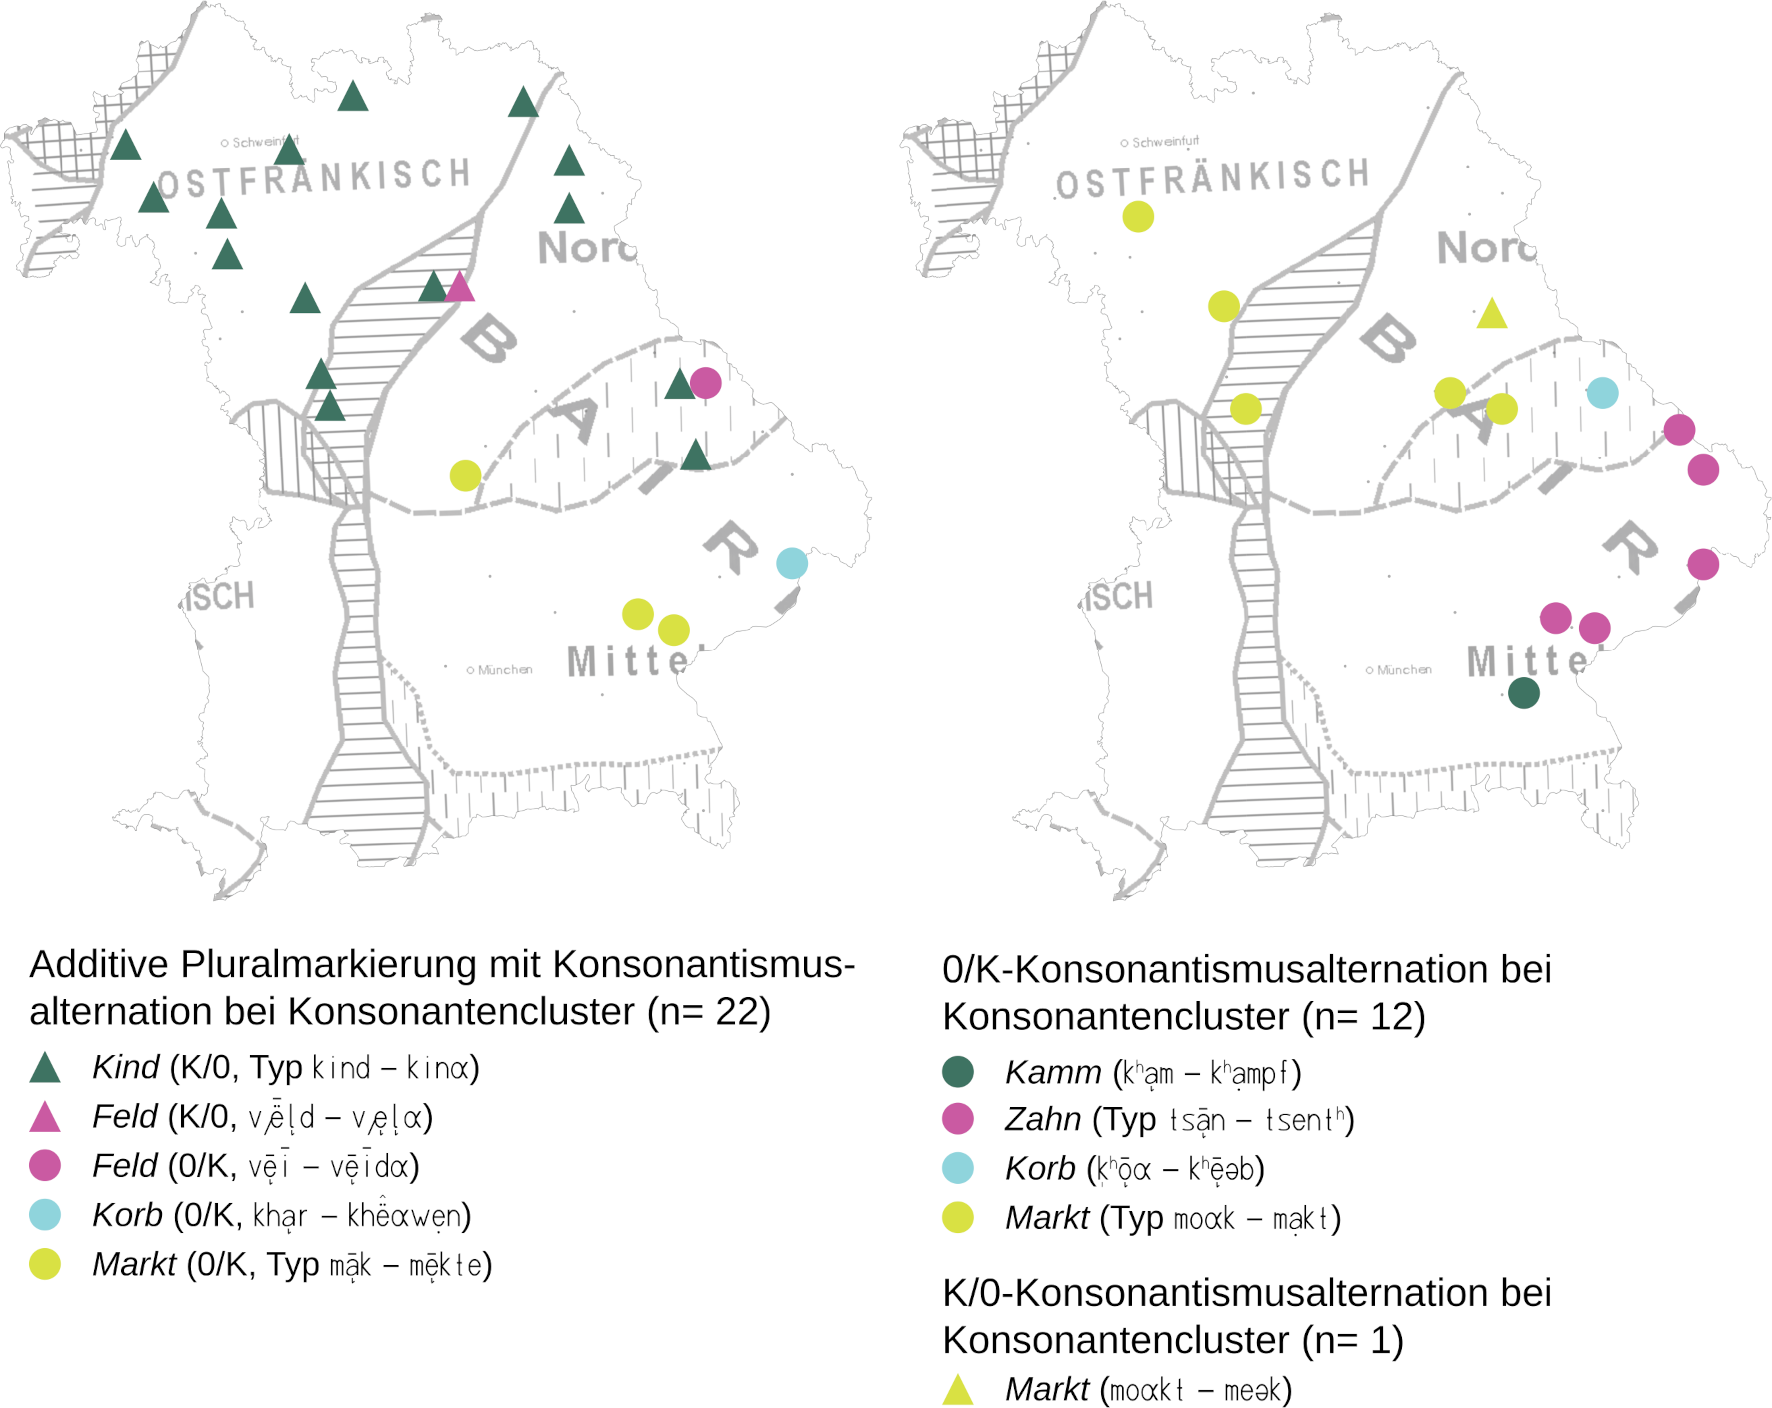
\includegraphics[width=\textwidth]{figures/Karte18.png}
\caption{Belege für Konsonantenelision bei Konsonantenclustern}
\label{map:18}
\end{map}


In stammaffizierenden Pluralformen treten innerparadigmatische Alternationen bei Konsonantenclustern eher im Bair. auf.\footnote{Nur für die Liquid+Plosivfolge in \textit{Markt} finden sich auch im Ofr. Formen mit elidiertem finalen /t/ in der Singularform von \textit{Markt} und erhaltenem /t/ im Plural (vgl. 	\tabref{tab:31}). \citet[127]{Roth1940} erwähnt daneben Fälle von Elision des auslautenden \textit{t} in der Umgebung von Fortisplosiven aus dem Egerländischen: \teuthoo{mo.Ek}{moͅək} ‚Markt‘, \teuthoo{lo.2Es}{lōͅəs} neben \teuthoo{lo.2sd}{lōͅsd} (Pl. \teuthoo{lo.isn4}{loͅisṇ}, ‚(Schuhmacher-)Leiste‘).} Trotz der geringen Belegdichte illustriert die Durchsicht von stammaffizierenden Markierungen bei Nasal-Plosiv-Abfolgen, in welchem Maße sich phonologische Prozesse und Pluralmarkierungsstrategien (respektive lexemspezifische Pluralformen) in den Dialekten bedingen. So ergeben sich im UG für die homorgane Sequenz aus Nasal und Dental in \textit{Kamm} (nhd. \textit{Kamm} < mhd. \textit{kamp} neben \textit{kam}, vgl. \citealt[I.783b]{Lexer1872-1878}) und \textit{Zahn} (ahd. \textit{zand}, mhd. \textit{zant} neben \textit{zan}, vgl. \citealt[III.848a]{Lexer1872-1878}) unterschiedliche Alternationsmuster mit erhaltenem vs. assimiliertem Finalplosiv je nach phontaktischer Position:\largerpage[-1]

\begin{itemize}
\item Für die /mb/-Abfolge in \textit{Kamm} erscheinen in einem Großteil der nieder-, mittel- und oberdeutschen Dialekte wie auch in der Standardsprache infolge der regelmäßig durchgeführten Assimilation des Labialplosivs im Aus- und Inlaut keine innerparadigmatische Alternation (Wechseltypus 0/0, z.\,B. \teuthoo{kha9.m}{kha\klammeruntenpost{}ͅm} -- \teuthoo{khe.m}{kheͅm} ‚Kamm‘, \teuthoo{khe94mA}{khe\klammeruntenpost{}̣mα} ‚kämmen‘ im ofr. Burgbernheim).
\item In Teilen des Ofr. (neben dem West- und Ostmitteldeutschen) ist die Assimilation von /mb/ in \textit{Kamm} nur im ehemaligen Inlaut (der additiven Pluralformen) durchgeführt, sodass synchron subtraktive Formen erscheinen: \teuthoo{kha."+mb\_}{khã̄ͅmbʰ} -- \teuthoo{khe.m}{kheͅm} ‚Kamm‘, \teuthoo{khemE}{khemə} ‚kämmen‘ im ofr.-hess. Wiesthal (vgl. \sectref{sec:7.1.2.4} sowie \citealt[76--78]{Birkenes2014}, \citealt[392--393]{Schirmunski1962}, \citealt[Karte 162]{SUF1}, \citealt[Karte 26]{SUF3}).
\item In konservativeren bair. Dialekten ist das Muster der Alternation ein anderes (mit anderen Worten: typisch bairisches), da das /b/ in der Finalposition im Singular assimiliert, in der Pluralform im sekundären Auslaut erhalten ist, z.\,B. \teuthoo{kha.m}{khaͅm} -- \teuthoo{kha4mb5\_}{khạmb̩ʰ} ‚Kamm‘, \teuthoo{k\_a94mb5e4n}{kʰa\klammeruntenpost{}̣mb̩ẹn} ‚kämmen‘ im nordbair.-mittelbair. Blaibach. Auch für die Nasal-Plosiv-Abfolge in \textit{Zahn} finden sich in Teilen des Bayerischen Waldes und des Rottals innerparadigmatische Alternationen durch Erhalt des ehemals intervokalischen /d/, z.\,B. \teuthoo{tSa2):n}{tʃā\klammeruntenpost{}{\doubleogonek}n} -- \teuthoo{tSe.nt\_}{tʃeͅntʰ} im nordbair.-mittelbair. Zwiesel (vgl. \citealt[§28c]{Kranzmayer1956}, \citealt[Karte 82]{SOB4}, \citealt[32 und 160]{SNiB4}).
\item Bei Erhalt des Plosivs auch im primären Auslaut erscheinen in den mittelbair. Tiefenbohrungspunkten lautgesetzlich entstandene Le\-nis-""For\-tis-""Kon\-tras\-te, z.\,B. \teuthoo{ka.<mb\%v\%}{kâͅmb͈v͈} -- \teuthoo{kha4mpf}{khạmpf} ‚Kamm‘ im mittelbair. Niedertaufkirchen, \mbox{\teuthoo{d5s5a.26d.}{d̩s̩ã̄ͅdͅ}} -- \teuthoo{tSe9.nt\_}{tʃe\klammeruntenpost{}ͅntʰ} im mittelbair. Waldhof.\footnote{Dass in den bair. Dialekten lexemweise eine hohe Varianz der formalen Realisierung \textrm{innerparadigmatischer Konsonantismusalternationen} im \textrm{interdialektalen Vergleich besteht,} zeigen auch \textrm{die Singular- und Pluralformen von} \textit{Korb}\textrm{. Ist der finale Plosiv der Liquid-Plosiv-Abfolge im Singular elidiert, in der (ehemals) intervokalischen Position des Plural aber erhalten, erscheinen innerparadigmatische Alternationen: \teuthoo{k,\_o.<A}{k͓ʰôͅα} -- \teuthoo{k\_e.<Eb5}{kʰêͅəb̩} im n}ordbair.-mittelbair. Grafenkirchen, \teuthoo{kha.r}{khaͅr} -- \teuthoo{khe>?Awe4n}{khë̂αwẹn} \textrm{im} mittelbair. Neukirchen am Inn. Ist der finale Plosiv in beiden Positionen erhalten, können innerparadigmatische Lenis-Fortis-Kontraste als Pluralmarkierungsstrategie funktionalisiert sein: \teuthoo{kho<Erb}{khôərb} -- \teuthoo{kherp}{kherp} im nordbair. Tirschenreuth.}
\end{itemize}

\subsubsubsubsection{Flexionsmorphologische Klassifikation der Obstruenten-Elision}
\begin{sloppypar}
Die konkrete formale Realisierung von stammaffizierenden Verfahren ist bei Stämmen mit auslautendem Obstruenten in hohem Maße durch das Eintreten (bzw. Nicht-Eintreten) von phonologischen Prozessen (Elision und Assimilation) bedingt. Da es hier für die einzelnen Lexeme im UG zum Teil großräumige, teilweise aber auch recht kleinräumige regionale Schwankungen gibt, ergibt sich ein ausgesprochen buntes Bild innerparadigmatischer Alternationen und der konkret belegten Pluralformen. Ist die Annahme eines Pluralmarkers „Konsonantismuskontrast“ hier sinnvoll, konstituiert er spezifische Deklinationsklassen? Für jene Fälle, die sich synchron „kaum auf einen gemeinsamen Nenner“ bringen lassen und regional stark schwanken, schlägt \citet[124]{Rowley1997} eine Klassifikation als (schwache) Suppletion vor.\footnote{\citet[217--218]{Schnabel2000} subsumiert in seiner synchronen Substantivklassifikation (die auch die Diminutivbildung einschließt) sogar Fälle als „schwache Suppletion“, die mit Blick auf die historisch-phonologische Entwicklung der Singular- und Pluralformen in dieser Arbeit als Konsonantismusalternationen (d.\,h. als stammaffizierende Markierung) gewertet werden würden, z.\,B. \teuthoo{gxI+"d}{ɡxı̃̄d} -- \teuthoo{gxine}{ɡxine} ‚Kind‘, \teuthoo{gxo+"b}{ɡxȭb} -- \teuthoo{gxem}{ɡxem} ‚Kamm‘, \teuthoo{bu2}{bū} -- \teuthoo{bum}{bum} ‚Bube‘.} Nur für das nordbair.-mittelbair. Übergangsgebiet im Bayerischen Wald führt \citet[124]{Rowley1997} so viele Fälle von innerparadigmatischer Konsonantenelision an, dass es „ökonomischer“ scheine, ein eigenes Flexionsmuster des Wechseltyps 0/K anzusetzen.
\end{sloppypar}

Alternativ zu dieser Klassifikation schlage ich eine Differenzierung innerparadigmatischer Konsonantismuselisionen bei additiven vs. stammaffizierenden Pluralmarkierungen vor, die die Formenbildung der Plural- und weniger die der Singularform fokussiert. 0/K-Alternationen in additiven Formen (Typ \teuthoo{vi“}{vī} -- \teuthoo{vi“cA}{vīXα}) sind -- ähnlich wie innerparadigmatische Spirantisierungen (\sectref{sec:7.1.2.3.3}) -- in stärkerem Maße phonologisch konditioniert, während 0/K- und K/0-""Al\-ter\-na\-tio\-nen als stammaffizierende Verfahren in den bair. Dialekten in kombinierten Markierungen (Typ \teuthoo{bao}{bao} -- \teuthoo{baeX}{baeꭗ}) oder als alleinige formale Marker der Pluralinformation (z.\,B. \teuthoo{we42}{wẹ̄} -- \teuthoo{we42g}{wẹ̄ɡ} ‚Weg‘ im nordbair.-mittelbair. Zwiesel) eher auf der morphologischen Ebene funktionalisiert sind. Damit ergibt sich für die bair. Dialekte ein spezifisches Flexionsmuster mit elidiertem Obstruenten im Singular und erhaltenem Obstruenten im Plural, die konkrete Realisierung ist dann möglicherweise lexemspezifisch im Lexikon abgespeichert.

\citet[19]{White1966} stellt bei jüngeren Sprechern des westmittelbair. Dialekts von Eisenhofen einen Abbau der innerparadigmatischen Alternationen zwischen elidiertem und erhaltenem Konsonanten fest („teils durch Systemzwang, teils infolge hochsprachlichen Einflußes“).\footnote{Bereits \citet[§111.2b]{Gebhardt1907} stellt den Abbau von Elisionen durch innerparadigmatischen Ausgleich für das Nürnberger Ofr. fest, z.\,B. in \textit{waib} ‚Weib‘, \textit{grob} ‚Grab’und \textit{loib} ‚Laib‘.} In additiven Pluralformen des Typs \teuthoo{we}{we} > \teuthoo{weg}{weɡ} -- \teuthoo{wega}{weɡa} ‚Weg‘ \citep[45]{White1966} entfällt durch den Dialektwandel zwar die innerparadigmatische Alternation, die Pluralform ist aber weiterhin distinkt. Es braucht weitere diachrone Daten, um zu zeigen, ob der Abbau des Dialektmerkmals auch in rein stammaffizierenden Formen des Typs \teuthoo{we42}{wẹ̄} -- \teuthoo{we42g}{wẹ̄ɡ} ‚Weg‘ stattfindet. Hier stellt die 0/-K-Alternation das einzige Pluralmerkmal dar, ein Abbau der Alternation würde den Wechsel in die Nullflexion bedeuten.

\subsubsubsubsection{Nasalelision}

Im gesamten UG (mit Ausnahme einiger Gebiete im Norden Bayerns, vgl. \citealt[59]{RennKönig2006}) ist die Elision von Nasal im Auslaut eingetreten (vgl. \citealt[§46]{Kranzmayer1956}, \citealt[125]{Rowley1997}, \citealt[112]{Roth1940}, \citealt[385]{Schirmunski1962}). Außer im Ofr. in Unterfranken und im Westen wird der Vokal „als Reflex des ursprünglichen Nasalkonsonanten“ (\citealt[59]{RennKönig2006}) nasaliert realisiert, z.\,B. \teuthoo{mo:"+}{mō{\doubleogonek}̃} ‚Mann‘ (nordbair. Nabburg), \teuthoo{s\#d\%o>+A+:"+}{šd͈ỗα̃̄{\doubleogonek}̃} ‚Stein‘ (mittelbair. Neukirchen am Inn).\footnote{Vgl. \citet[74]{Rowley1997}, \citet[128]{Schmeller1821} sowie \citet[11]{Schießl1909} zum Mittelbair. und zum Ofr. \citet[§95.1]{Gebhardt1907}.}  Erhalt vs. Elision des auslautenden Nasals wurde getrennt für die mhd. Kurz- und Langvokale und Diphthonge untersucht, da die Nasaltilgung sowohl in der Stellung nach kurzem wie langem Vokal für einzelne Wörter und „je nach der grammatischen Form und Funktion“ \citep[385]{Schirmunski1962} unterschiedlich erfolgt ist.

Für die mhd. Kurzvokale (im Korpus belegt sind nur Substantive mit Stammvokal mhd. \textit{a}) zeigt sich, dass die Art des Pluralmarkierungsverfahrens (additiv vs. rein stammaffizierend) den Erhalt bzw. die Tilgung des Nasals bedingt (vgl. \citealt[125]{Rowley1997}). Für \textit{Zahn} (mhd. \textit{zant}, \textit{zan}), das den Plural im UG durch Umlaut markiert, sind nur Formen ohne innerparadigmatische konsonantische Alternation als Wechseltypus 0/0 (Typ \teuthoo{dso2}{dsō} -- \teuthoo{dse2}{dsē} im Ofr. und Nordbair.) oder K/K (Typ \teuthoo{dsa2n}{dsān} -- \teuthoo{dse2n}{dsēn} im Mittelbair.) realisiert. (Ausgenommen werden hier die mittelbair. Formen mit Dentalplosiv im Auslaut, die innerparadigmatische Alternation durch Plosivelision aufweisen, vgl. \mapref{map:18}). Für das additiv-modulative Pluralverfahren des Belegworts \textit{Mann} wird in allen Ortspunkten die Singularform mit elidiertem Nasal, die Pluralform mit Nasal und Pluralsuffix realisiert, z.\,B. \teuthoo{ma."+}{mã̄ͅ} -- \teuthoo{ma."+nA}{mã̄ͅnα} (mittelbair. Waldhof, vgl. \citealt{WA}-Karte 46 „Mann“). Der Stammvokal der Singularform ist gedehnt, was nach \citet[385]{Schirmunski1962} mit der Nasalelision in der Stellung nach kurzem Vokal einhergeht, im Plural erscheint in den bair. Ortspunkten analogischer Langvokal. In den ofr. Ortspunkten wird im Plural Kurzvokal realisiert (z.\,B. \teuthoo{mo42+}{mọ̄̃} -- \teuthoo{me4nE}{mẹnə} in Wilhermsdorf), sodass es neben Kontrasten der Vokalqualität (Umlaut) auch Kontraste der Vokalquantität zwischen Singular und Plural gibt.


\begin{map}
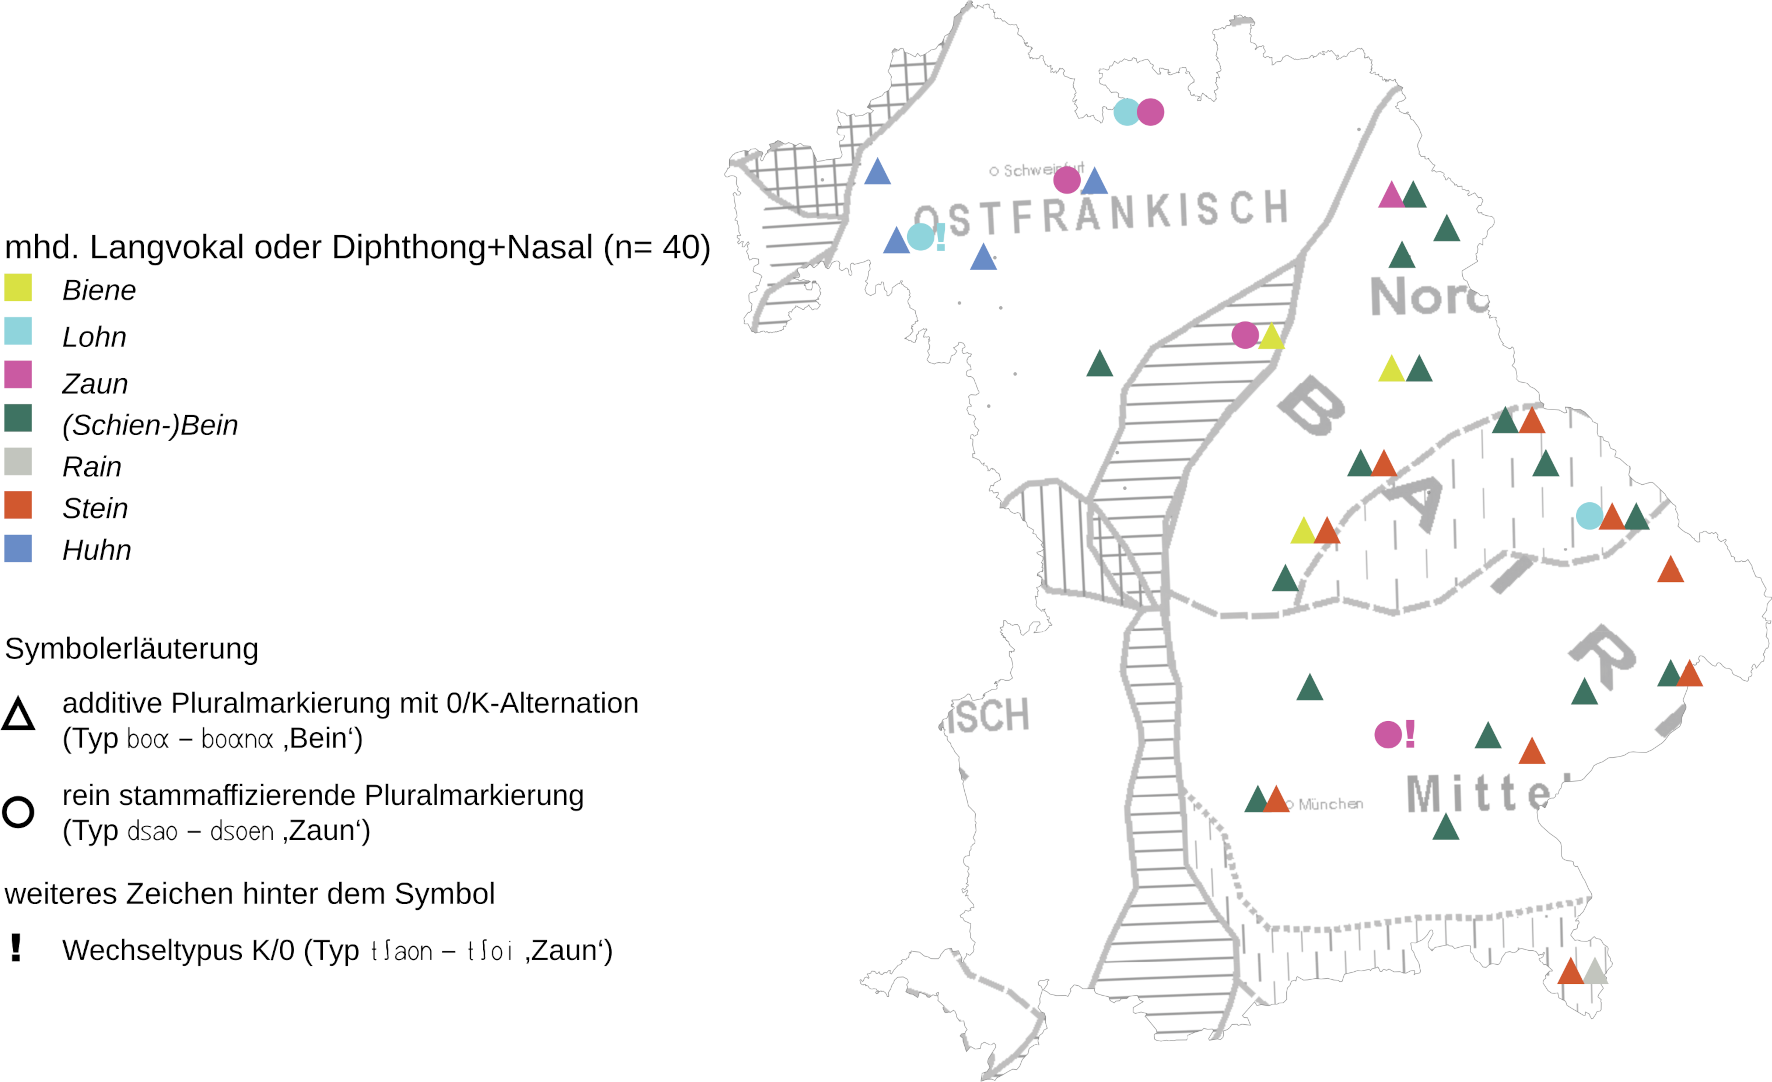
\includegraphics[width=\textwidth]{figures/Karte19.png}
\caption{Innerparadigmatischer Wechsel bei Nasalelision nach mhd. Langvokal und Diphthong im primären und sekundären Auslaut}
\label{map:19}
\end{map}

Auch bei den Substantiven mit mhd. Langvokal oder Diphthong im Stammvokal bedingt v.\,a. das Pluralverfahren, ob der Nasal in der Pluralform realisiert wird (vgl. \citealt{WA}-Karte 224 „Wein“): 83\,\% der Belege mit Nasalelision im Singular markieren den Plural additiv (neben möglicher Vokalmodulation), nur sieben der 40 Fälle (17\,\%) bilden die Pluralform durch ein rein stammaffizierendes Verfahren. \mapref{map:19} zeigt, dass innerparadigmatische Nasalelision lexemweise größere Areale umfasst und ortsdialektspezifisch sein kann.\footnote{Der Nasal nach mhd. \textit{ei} wird in den bair. Tiefenbohrungspunkten im Lexem \textit{Bein} (bzw. \textit{Schienbein}) im Singular überwiegend elidiert, im Mittelbair. und nordbair.-mittelbair. Übergangsgebiet außerdem bei \textit{Stein} sowie als Einzelbeleg \textit{Rain}. In anderen phonologischen Umgebungen (respektive Lexemen) tritt Nasal\-elision nur in einem kleinen Gebiet auf: \textit{Huhn} im Unterofr., \textit{Biene} vereinzelt im Nordbair. Es finden sich außerdem vereinzelte Belege für Nasaltilgung bei \textit{Lohn} und \textit{Zaun} (mit K/0-Alternation im mittelbair. Inning am Holz).} Daneben wird bei Einsilbern in der phonologischen Umgebung vor auslautendem Obstruenten (meist bei eingetretener Einsilberdehnung) der Nasal in einem Teil des UG in der Singularform elidiert: in einem relativ großen Areal im Ofr. und Mittelbair. bei \textit{Gans} sowie vereinzelt im Mittelbair. bei \textit{Gang}, \textit{Kind, Sense} und \textit{Zahn} (mit erhaltenem Plosiv im primären und sekundären Auslaut), z.\,B. \teuthoo{go:2s}{ɡo{\doubleogonek}̄s} (neben \teuthoo{ga):"(+nds}{ɡã̄{\doubleogonek}\klammerobenpost{}\klammeruntenpost{}nds}) -- \teuthoo{gends59}{ɡends̩\klammeruntenpost{}} ‚Gans‘ (ofr. Krum),\footnote{Das auslautende /s/ wird hier als Affrikate realisiert. \citet[§34h1]{Kranzmayer1956} beschreibt das epenthetische [d] zwischen Nasal oder Liquid und Frikativ für das Bair., insb. nach Kurzvokal sei die Epenthese „gemeinbair.“, vgl. Sg. \teuthoo{go.2ns}{ɡōͅns} vs. Pl. \teuthoo{ge.ntß}{ɡeͅntß} im Nord- und Mittelbair.} \teuthoo{s5a4>+s\%d\%\_}{s̩ậ̃s͈d͈ʰ} -- \teuthoo{s\%a4ns5n@}{s͈ạns̩n̥} ‚Sense‘ (mittelbair. Neukirchen am Inn).\footnote{Im Mittelbair. ist Nasalelision außerdem belegt bei \textit{Gang}, \textit{Kind,} und \textit{Zahn} (mit erhaltenem Plosiv im primären und sekundären Auslaut), z.\,B. \teuthoo{ga:"+g.}{ɡā{\doubleogonek}̃ɡͅ} -- \teuthoo{ga4N}{ɡạŋ} ‚Gang‘ (nordbair.-mittelbair. Grafenkirchen), \teuthoo{A}{α} \teuthoo{gás\%und5s5}{ɡ͈s͈und̩s̩} \teuthoo{khi4"4d5}{khị̣̄d̩} -- \teuthoo{k,hindA}{k͓hindα} ‚Kind‘ (mittelbair. Neukirchen am Inn), \teuthoo{d5s5a.26d.}{d̩s̩ã̄ͅdͅ} -- \teuthoo{tSe9.nt\_}{tʃe\klammeruntenpost{}ͅntʰ} ‚Zahn‘ (mittelbair. Waldhof). \citet[75, 125]{Rowley1997} führt außerdem Belege für \textit{Band, Hund} und \textit{Kamm} in Nordbayern an (vgl. \citealt{WA}-Karte 179 „Kind“ und 532 „Hund“; \citealt[§46e und Karte 23]{Kranzmayer1956}, \citealt[16/112]{Roth1940}, \citealt[74 und Karte 16]{Rowley1997}).}

\vfill
\begin{table}[H]
\begin{tabular}{lllll}
\lsptoprule
& {Singular} & {Plural} & {Diminutiv} & \\\midrule
Dorn\footnote{In Erlabrunn mit Nullmarkierung im Pl. (\teuthoo{do42rA94}{dọ̄rα\klammeruntenpost{}̣} - \teuthoo{do42rA94}{dọ̄rα\klammeruntenpost{}̣}).} & \teuthoo{do.2ArE.}{dōͅαrəͅ} & \teuthoo{do.<AnA94}{dôͅαnα\klammeruntenpost{}̣} &  & Gebsattel\\
& \teuthoo{do.2rE.}{dōͅrəͅ} & \teuthoo{dôo?:rnEr}{d{\aufstrih}ö{\doubleogonek}rnər} &  & Ochsenfurt\\
\tablevspace
Horn & \teuthoo{ho.2ArE.}{hōͅαrəͅ} & \teuthoo{h{\textasciitilde}ôo?.rnEr}{h{\aufstrih}öͅrnər} &  & Erlabrunn\\
& \teuthoo{h{\textasciitilde}ôo.2urE}{h{\aufstrih}ōͅurə} & \teuthoo{h{\textasciitilde}ôo.2urE}{h{\aufstrih}ōͅurə}, \teuthoo{hÔe.rnEr}{h{\doppelaufstrih}eͅrnər} & \teuthoo{hElE.}{hələͅ} & Gebsattel\\
& \teuthoo{ho.2rE}{hōͅrə} & \teuthoo{ho?.EnEr}{höͅənər} &  & Ochsenfurt\\
\tablevspace
Kern\footnote{In Gebsattel und Ochsenfurt mit Nullmarkierung im Pl.} & \teuthoo{k\_e.2rE}{kʰēͅrə} & \teuthoo{k\_e.<AnE}{kʰêͅαnə} &  & Gebsattel\\
\tablevspace
Korn & \teuthoo{khôo.2rE}{kh{\aufstrih}ōͅrə} & \teuthoo{kho?.rnE.y}{khöͅrnəͅ⅄} & \teuthoo{khôo>?:E.lE}{kh{\aufstrih}ö̂{\doubleogonek}əͅlə} & Erlabrunn\\
\lspbottomrule
\end{tabular}
\caption{Innerparadigmatische Alternation durch Nasalelision im westlichen Ofr.}
\label{tab:36}
\end{table}
\vfill\pagebreak

Im westlichen Ofr. findet sich für eine kleine Gruppe von Lexemen (\textit{Dorn}, \textit{Horn}, \textit{Kern}, \textit{Korn}) ein dialektraumspezifisches Muster innerparadigmatischer Alternationen (\tabref{tab:36}). In historischen Einsilbern kann hier (wie auch im Schwäbischen) in der phonologischen Umgebung /r/ vor Nasal im Auslaut ein epenthetisches Schwa erscheinen.\footnote{Vgl. \citealt[120 und Karten 60--61]{SBS3}, \citet[389]{Schirmunski1962}, \citealt[Karte 7]{SMF7}, \citealt{WA}-Karte 553 „Korn“; \citet[Karte 18]{Fischer1895}.} In den durch die Epenthese entstandenen zweisilbigen Formen wird der auslautende Nasal elidiert (bei gleichzeitiger Dehnung des Stammvokals in offener Tonsilbe, vgl. \citealt[120]{SBS3}). Da die Schwa-Epenthese nur historische Einsilber betraf, erscheint synchron eine innerparadigmatische Alternation zwischen Epenthese und Nasalelision im Singular und Nasalerhalt im Plural\footnote{In diese Reihe von Substantiven mit /r/-Nasal-Abfolge im Auslaut gehören ebenso \textit{Birne}, \textit{Stern}, \textit{Turm} (wobei \textit{Birne} kein „Sprossvokalwort“ ist, sondern auf mhd. \textit{bir(e)} zurückgeht, sich aber wie ehemalige Einsilber mit -\textit{rn}{}-Folge und Sprossvokal verhält, \citealt[120 und 154]{SBS3}). Die Pluralformen werden in den genannten Ortsdialekten jeweils mit Nullmarkierung bildet. Die Substantive \textit{Arm,} \textit{Darm} und \textit{Wurm} sind in den drei Ortspunkten jeweils mit konsonantischem Auslaut und ohne Sprossvokal belegt; nur im ebenfalls unterofr. Stadtschwarzach erscheint \textit{Arm} im Singular mit elidiertem Nasal (\teuthoo{a4rE}{ạrə} -- \teuthoo{arEm}{arəm}, aber \teuthoo{e.r}{eͅr} \teuthoo{ho.d}{hoͅd} \teuthoo{si.}{siͅ} \teuthoo{E.}{əͅ} \teuthoo{a.m}{aͅm} \teuthoo{gEbro4xN}{ɡəbrọxŋ}) und \textit{Darm} mit epenthetischem Schwa (\teuthoo{da4rEm}{dạrəm} -- \teuthoo{de.rmEr}{deͅrmər}, aber \teuthoo{a4r}{ạr} \teuthoo{ho.ds}{hoͅds} \teuthoo{i.}{iͅ} \teuthoo{dEr}{dər} \teuthoo{da4rm}{dạrm}).}

Die Zusammenschau aller Formen zeigt, dass innerparadigmatische Alternationen zwischen elidiertem vs. erhaltenem Nasal vor allem in additiven Pluralformen auftreten. Wie auch in den vorangegangenen Kapiteln zur innerparadigmatischen Alternation bei Obstruenten stellt sich die Frage: Wie können die verschiedenen Fälle aus flexionsmorphologischer Perspektive modelliert werden? Die Darstellung der lauthistorischen Entwicklung verdeutlicht, dass es sich einerseits um kleinräumige, dialektraumspezifische Entwicklungen handelt und dass die Alternation nur für eine kleine Gruppe von Lexemen gilt (vgl. die Nasalalternation des Typs \teuthoo{do2rE}{dōrə} -- \teuthoo{do?rnEr}{dörnər} im westlichen Ofr. und die stamminlautende Alternation des Typs \teuthoo{go2s}{ɡōs} -- \teuthoo{gens}{ɡens} im Ofr. und Mittelbair.). Für diese Fälle scheint \citegen[125]{Rowley1997} Klassifikation als „ein eigenes Flexionsmuster mit beschränkter Besetzung“ sinnvoll.


\begin{table}
\small
\begin{tabularx}{\textwidth}{QQ>{\raggedright\arraybackslash}p{.3\textwidth}p{.2\textwidth}}
\lsptoprule
{Singular} & {Plural} & &\\
\midrule
 \teuthoo{se.2X}{sēͅꭗ} & \teuthoo{se.2NA}{sēͅŋα} & ‚Säge‘ (Kallmünz) & \multirow[t]{2}{=}{Südl. Nordbair.}\\
 \teuthoo{nôo(+u(+d5}{n{\aufstrih}õ\klammerobenpost{}ũ\klammerobenpost{}d̩} & \teuthoo{nôo(+u(+nA}{n{\aufstrih}õ\klammerobenpost{}ũ\klammerobenpost{}nα} & ‚Naht‘ (Oberdolling) & \\
 \midrule
 \teuthoo{wo4<Na4kS}{wộŋạkʃ} & \teuthoo{wo4<Na4kSn@A}{wộŋạkʃn̥α} & ‚Achse‘ (Grafenkirchen) & \multirow[t]{4}{=}{Nordbair.-Mittelbair. Übergangsgebiet}\\
 \teuthoo{gbma4end5e4}{ɡbmạend̩ẹ} & \teuthoo{gbma4end5e4NA}{ɡbmạend̩ẹŋα} & ‚Gemeinde‘ (Blaibach) & \\
 \teuthoo{muEt,E}{muət͓ə} & \teuthoo{mu<EdAnE}{mûədαnə} & ‚Mutter‘ (Bernhardswald) & \\
 \teuthoo{bmuAtA}{bmuαtα} & \teuthoo{muAdAnA}{muαdαnα} & ‚Mutter‘ (Blaibach) & \\
 \midrule
 \teuthoo{A}{α} \teuthoo{d5e."+nA}{d̩ẽ̄ͅnα} & \teuthoo{de.>+nAne4}{dễͅnαnẹ} & ‚Tanne‘ (Grafenau) & \multirow[t]{2}{=}{Mittelbair.}\\
 \teuthoo{{d5}e}{d̩e} \teuthoo{d5i“4A}{d̩ị̄α} & \teuthoo{d5i“4AnA}{d̩ị̄αnα} & ‚Tür‘ (Kirchensur) & \\
 \tablevspace
 \teuthoo{E}{ə} \teuthoo{no\$i\^{}i:@}{nō̤{\aufstrih}i{\doubleogonek}} \teuthoo{gJo4kH}{ɡ{\lkreis}ọkhͯ} & \teuthoo{no\$i\^{}i:}{nō̤{\aufstrih}i{\doubleogonek}} \teuthoo{gJo4kHNA}{ɡ{\lkreis}ọkhͯŋα} & ‚Glocke‘ (Ramsau) & \multirow[t]{4}{=}{Mittelbair.-Südbair. Übergangsgebiet}\\
 \teuthoo{gmo>+A}{ɡmỗα} & \teuthoo{gmo2A2nA}{ɡmōᾱnα} & ‚Gemeinde‘ (Ramsau) & \\
 \teuthoo{fui.}{fuiͅ} & \teuthoo{fu9.i9.nA}{fu\klammeruntenpost{}ͅi\klammeruntenpost{}ͅnα} & ‚Furche‘ (Ramsau) & \\
 \teuthoo{s5a4<i:}{s̩ậi{\doubleogonek}} & \teuthoo{s5a4<i:nA}{s̩ậi{\doubleogonek}nα} & ‚Säule‘ (Ramsau) & \\
\lspbottomrule
\end{tabularx}
\caption{Pluralmuster Nasal+Tiefschwa der Feminina im Bair.}
\label{tab:37}
\end{table}

Für die meisten der additiven Pluralformen nehme ich indes ein eigenes Pluralbildungsmuster an, das -- zumindest für Feminina -- als solches auch kognitiv verankert und produktiv scheint, aber in der bisherigen Darstellung zur Nasalelision gefehlt hat. Dieses Muster entspricht auf der Formebene den „Doppelsuffigierungen“ des Typs \teuthoo{s\#tum}{štum} -- \teuthoo{s\#tumA}{štumα} ‚Stube‘ der zweisilbigen Feminina mit Nasalsuffix in der Singularform (vgl. \sectref{sec:7.1.1.3}). \citet[154]{Rowley1997} setzt hier eine Teilklasse Nasalsuffix im Plural mit Nasalschwund im Singular an, z.\,B. \teuthoo{mas\#i}{masī} -- \teuthoo{mas\#I2na}{mašı̄na} ‚Maschine‘, \teuthoo{rosI2}{rosı̄} -- \teuthoo{rosI2na}{rosı̄na} ‚Rosine‘. Auch die innerparadigmatische Nasalalternation in der Pluralform \teuthoo{gmo>+A+}{ɡmỗα̃} -- \teuthoo{gmo2A2nA}{ɡmōᾱnα} ‚Gemeinde‘ (mittelbair.-südbair. Ramsau) klassifiziert \citet[154]{Rowley1997} als Nasalelision des Typs 0/K.

In 	\tabref{tab:37} sind weitere Belege aus den bair. Tiefenbohrungspunkten aufgeführt, die diesem Muster ähneln. Es handelt sich um ein- oder zweisilbige Feminina, deren Singularstammformen unterschiedlich gebildet sind. Es gibt apokopierte Stämme, Stämme mit vokalisch realisierter \textit{n}{}-Erweiterung sowie die irregulär flektierenden Substantive \textit{Gemeinde}, \textit{Naht} und \textit{Mutter}.\footnote{Daneben wird im Ofr. und nördlichen Nordbair. der Nasal im Auslaut des unbetonten Movierungssuffixes -\textit{in} in \textit{Bäuerin} und \textit{Näherin} im Singular elidiert, in den additiven Pluralformen ist er vor dem Pluralsuffix erhalten, z. B. \teuthoo{ba4<e\$i\^E.ri.}{bậe̤ï̯əͅriͅ} -- \teuthoo{ba4<e4i\^E.ri.nA4}{bậẹi̯əͅriͅnα̣} (ofr. Wilhermsdorf), \teuthoo{na42dEre4.}{nạ̄dərẹͅ} -- \teuthoo{na2dEri.-nEn}{nādəriͅ{}͐nən} (nordbair. Tirschenreuth, vgl. \sectref{sec:8.3.4}).} Die Pluralformen dieser heterogenen Gruppe an Feminina entsprechen jeweils dem Muster Nasal+Tiefschwa. Da sich der Nasal historisch nicht durch den primären Stammauslaut erklären lässt (evtl. mit Ausnahme von \textit{Gemeinde} nach der Analyse von \citealt[154]{Rowley1997}), erscheint die Annahme eines eigenen Pluralbildungsmusters plausibel. Auf der Formebene entsprechen diese Plurale einer Art Doppelsuffigierung aus Nasal und vokalischem Pluralsuffix, sodass es hier -- trotz unterschiedlicher Tiefenstruktur -- sinnvoll erscheint, ein eigenes Flexionsmuster, also eine genusspezifische Plural-Outputstruktur der Feminina im Bair. anzunehmen (ausführlicher hierzu \sectref{sec:8.3.3.1}).

\subsubsubsection{Spirantisierung}
\label{sec:7.1.2.3.3}
In weiten Teilen des UGs wird mhd. \textit{b} im Auslaut als labialer Plosiv, im Inlaut zwischen zwei Vokalen und zwischen Vokal und Sonant als (bi-)labialer Frikativ realisiert: \teuthoo{go2bl@}{ɡōbl̥} vs. \teuthoo{go2wl@}{ɡōwl̥} ‚Gabel‘, \teuthoo{waebA}{waebα} vs. \teuthoo{waewA}{waewα} ‚Weiber‘. Durch die Spirantisierung (auch Frikativierung, vgl. \citealt[197]{Streck2012}) in intervokalischer Position ergibt sich in Flexionsformen ein innerparadigmatischer Wechsel \textit{b>w}, z.\,B. \teuthoo{gro9.2b}{ɡro\klammeruntenpost{}̄ͅb} -- \teuthoo{gra42wA}{ɡrạ̄wα} (mittelbair. Kirchensur).\footnote{Vgl. \citet[29f.]{Lessiak1933}, \citet[§25b/30b]{Kranzmayer1956}, \citet[69]{RennKönig2006}, \citet[79]{Rowley1997}, \citet[304]{Schirmunski1962}, \citet[218--219]{Steger1968}, \citet[453]{Wiesinger1990}.} \mapref{map:20} illustriert, dass die Spirantisierung von /b/ gleichermaßen in den ofr. und bair. Tiefenbohrungspunkten vorkommt, dass v.\,a. in den bair. Ortsdialekten die Singularform mit elidiertem Plosiv im Auslaut, die Pluralform mit erhaltenem und in intervokalischer Position spirantisiertem /b/ realisiert wird, z.\,B. \teuthoo{wâa<e\$<}{w{\aufstrih}âê̤} -- \teuthoo{twâa4<e\$+wA4}{tw{\aufstrih}ậẽ̤wα̣} ‚Weib‘ (mittelbair. Inning am Holz) oder \teuthoo{bu2A}{būα} -- \teuthoo{bu2AwE.4}{būαwə̣ͅ} ‚Bube‘ (ofr. Erlabrunn; vgl. \sectref{sec:7.1.2.3.2} zur Elision und \citealt[§30b3]{Kranzmayer1956}).\footnote{Die Variation in der arealen Distribution der einzelnen Lexeme mit stammauslautendem /b/ ergibt sich hier primär daraus, dass einzelne Lexem nicht im gesamten UG belegt sind (so etwa \textit{Sieb}, \textit{Kalb} wurde daneben vor allem in der Diminutiv-Form im Singular und Plural realisiert), daneben sind in anderen (grundsätzlich spirantisierenden) Ortsdialekten lexemweise keine additiven Pluralmarkierungen belegt (so etwa bei \textit{Laib}).}


\begin{map}
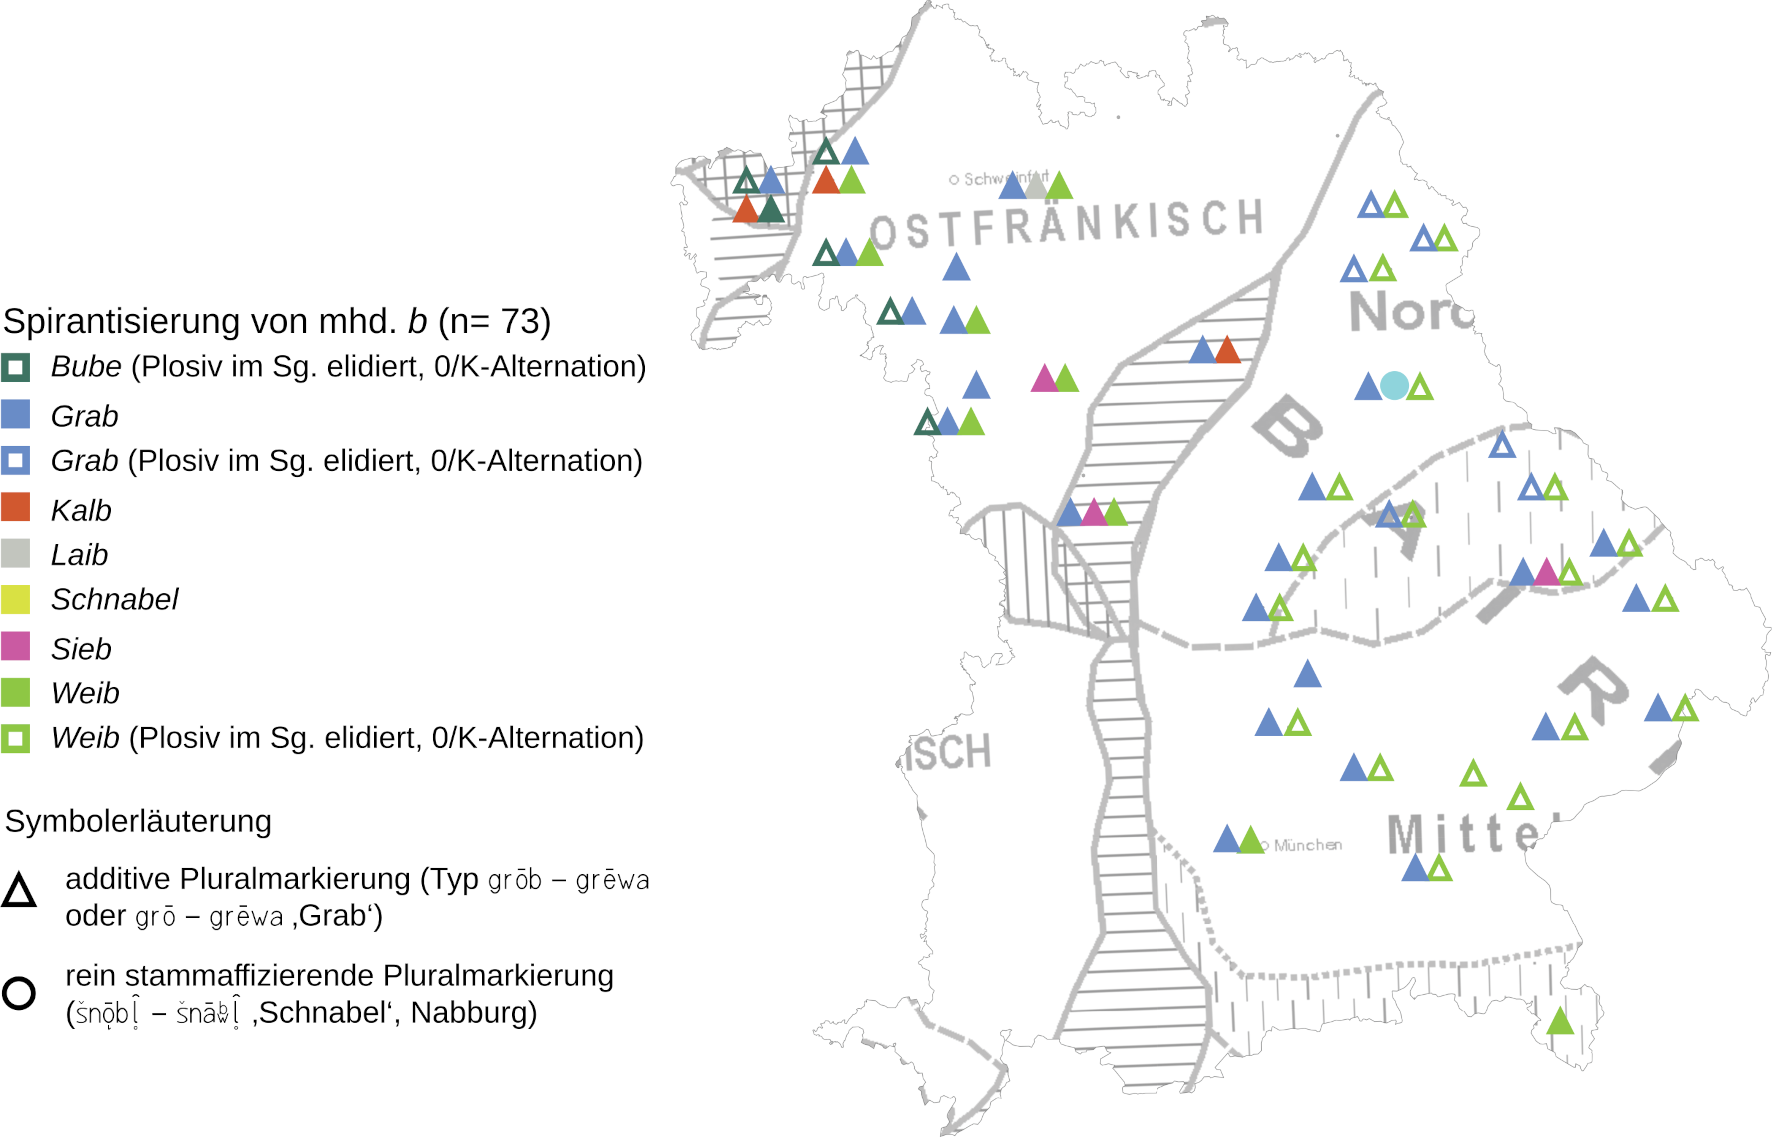
\includegraphics[width=\textwidth]{figures/Karte20.png}
\caption{Spirantisierung von intervokalischem /b/}
\label{map:20}
\end{map}

Spirantisierungen von intervokalischem /b/ in additiven Pluralformen stellen einen Fall kombinatorischer (positionsbedingter) Allophonie dar (vgl. \citealt[125]{Rowley1997}). Anders liegt der Fall bei der Spirantisierung von mhd. \textit{g} und mhd. \textit{c} (aus ahd. \textit{g} in Auslautverhärtung, vgl. \citealt[218--219]{SMF4}), da laut \citet[125]{Rowley1997} die in den Dialekten belegten Minimalpaare die Lösung als Allophonie „verbieten“. Mhd. \textit{g} und mhd. \textit{c} werden im ofr. und nordbair. Teil des UGs je nach Lautumgebung im Inlaut meist spirantisiert, im mittelbair. Teil nicht-spirantisiert (d.\,h. plosivisch) realisiert.\footnote{Im Ofr. erfolgt im In- und Auslaut weitestgehend Zusammenfall, im Nordbair. teilweiser Zusammenfall von mhd. \textit{g} und \textit{ch}, vgl. z.\,B. die Homonymie bei \textit{Tag} und \textit{Dach} in ofr. Erlabrunn (\teuthoo{da2x}{dāx}) und nordbair. Groschlattengrün (\teuthoo{do42X}{dọ̄ꭗ}, vgl. \citealt[Karte 29]{Gütter1971}, \citealt[§29]{Kranzmayer1956}, \citealt[79]{Rowley1997}, \citealt[216--219]{SMF4}, \citealt[241--250]{Steger1968}).} Im gesamten Datenmaterial gibt es nur zwei Belege für die innerparadigmatische Alternation durch Spirantisierung bei mhd. \textit{(c)h}. Im mittelbair. Inning am Holz wird auslautendes [g] in intervokalischer Position zu [x] in spirantisiert: \teuthoo{vu\$rgá\_}{vṳrɡ͈ʰ} -- \teuthoo{vu.yxA4n}{vuͅ⅄xα̣n} ‚Furche‘ (mhd. \textit{vurch}). Diese innerparadigmatische Alternation findet sich vereinzelt auch in umliegenden Ortsdialekten (vgl. \citealt[177 und Karten 40/41]{SNiB7}, \citealt[Karte 86]{SOB4}).\footnote{Auf Alternationen im Konsonantismus wurde bei der Typisierung der Singular- und Pluralformen (respektive der Pluralmarker) in der Auswertung und im Kommentar des SOB nicht eingegangen; die \textit{BayDat}-Vollformen-Karte im REDE-SprachGis zeigt aber, dass es auch hier Alternationen durch Spirantisierung zumindest vereinzelt gibt. Daneben findet sich im ofr.-nordbair. Mitteleschenbach (und bei weiteren Belegen im südlichen ofr.-nordbair. Übergangsgebiet) die innerparadigmatische Alternation zwischen Frikativ im Auslaut und plosivischer Realisierung vor Nasalsuffix bei \teuthoo{h{\textasciitilde}ôe.i.c}{h{\aufstrih}eͅiͅꭗ} -- \teuthoo{he.i.gN}{heͅiͅgŋ} ‚Höhe‘ (mhd. \textit{hœhe}, \textit{hœch}, vgl. \citealt[273]{SMF4}).} 

Spirantisierungen sind als morphophonologische Alternation auf der in der Einführung von \chapref{chap:7} vorgeschlagenen Skala zwischen den Polen lexikalisierte vs. produktive morphophonologische Alternationen zu verorten. Die Spirantisierung von /b/ ist aus synchronen phonologischen Regeln ableitbar und erscheint nur in additiven Pluralformen;\footnote{Die Spirantisierung der einzigen stammaffizierenden Pluralform in \mapref{map:20}, \teuthoo{s\#no.2bl@°}{šnōͅbl̥̑} -- \teuthoo{s\#na2æl@°}{šnā{\burgerbw}l̥̑} ‚Schnabel‘ im nordbair. Nabburg, ist als „Burger“ aus [b] und bilabialem Frikativ [w] im Plural transkribiert. Diese Zwischenwertnotation wurde gemäß den in \sectref{sec:6.3.1.2} dargestellten Typisierungsrichtlinien dem unteren Bestandteil zugeordnet und damit als Spirantisierung annotiert. Ich werte diese Realisierung eher als Beleg der graduellen Realisierung phonetischer Merkmale (hier von Spirantisierung) und weniger als Funktionalisierung als Pluralmarker.} damit liegt kein produktives Kodierungsverfahren vor. Die Spirantisierung von mhd. \textit{(c)h} scheint noch stärker lexikalisiert zu sein. Im Folgenden werden v.\,a. Spirantisierungen von /b/ trotz ihrer phonologischen Bedingtheit als morphologisch relevant berücksichtigt, da die Spirantisierung des Stammauslauts in Pluralformen des Typs \teuthoo{gro2b}{ɡrōb} -- \teuthoo{gre2wA}{ɡrēwα} ‚Grab‘ das folgende Pluralsuffix indiziert. Die Kookkurrenz von Konsonantismusalternation und Pluralsuffix symbolisiert als Ganzes die Pluralinformation, auch wenn es eine „Asymmetrie“ \citep[194]{Ronneberger-Sibold1990} zwischen beiden Einheiten gibt, da die Spirantisierung nicht distinktiv ist (siehe aber \sectref{sec:8.1} zur Konkomitanz von Spirantisierung und Suffix).

Ausgangspunkt dieser Überlegungen ist \citegen[194--201]{Ronneberger-Sibold1990} Modellierung der semiotisch-kommunikativen Rolle des Umlauts und seiner Verselbstständigung als distinktives Zeichen im Laufe des Sprachwandels. Im Falle der Spirantisierung liegt synchron zwar keine „Verselbstständigung“ vor, sie ist in den rezenten Dialekten phonologisch bedingt und damit Begleiterscheinung des Pluralsuffixes, doch ist die semiotische Funktion m.\,E. vergleichbar. Der Vorteil dieser Lösung besteht in meinen Augen darin, dass die phonologische und die morphologische Ebene sowohl in der mentalen Repräsentation als auch in der Perzeption nicht künstlich (nämlich durch ein linguistisches Modell von modularen Ebenen im Sprachsystem) voneinander geschieden werden.

\subsubsection{Subtraktion}
\label{sec:7.1.2.4}
Subtraktive Morphologie besteht in der Kürzung einer Wortform, d.\,h. in der Tilgung von phonologischem Material, um morphologische Information zu kodieren (vgl. \citealt[21]{Birkenes2014}, \citealt[581]{Dressler2000}, \citealt[143]{GolstonWiese1996}). \citet[582]{Dressler2000} versteht unter einer prototypischen Subtraktion „a reductive grammatical morphological process“: Der synchrone morphologische Prozess bestehe in der Reduktion eines Phonems am rechten Rand der Basis, zugleich symbolisiert die Subtraktion als einziger overter Marker eine morphologische Bedeutung (z.\,B. die Pluralinformation). Fälle nicht-prototypischer Subtraktion lassen sich definitorisch weniger eindeutig fassen, sie bestehen beispielsweise in der Reduktion von mehr als einem Phonem oder von weniger als einem Phonem, d.\,h. von einzelnen Phonemmerkmalen, beispielsweise in Form einer Vokalkürzung (bzw. im Schwund einer More, vgl. \citealt[25]{Birkenes2014}, \citealt[582]{Dressler2000}). Ich verwende im Folgenden die enge Definition von (prototypischer) Subtraktion, weshalb Kontraste der Vokalquantität als eigenständige Belege stammaffizierender Morphologie klassifiziert werden (vgl. \sectref{sec:7.1.2.2}).

Ob Singular- und Pluralformen des Typs \teuthoo{khe2nd}{khēnd} -- \teuthoo{khen}{khen} ‚Kind‘ (ofr.-hess. Wiesthal) tatsächlich einen synchronen morphologischen Prozess der Subtraktion im Deutschen und seinen Dialekten belegen, wurde in der Literatur kontrovers diskutiert (vgl. hierzu die Diskussion in \citealt[31--33]{Birkenes2014}). Nach \citet[582]{Dressler2000} setzt die Definition von Subtraktion als morphologischem Prozess „some minimum generality and regularity“ voraus. Letztlich, so \citet[583]{Dressler2000}, hänge der Status der subtraktiven Morphologie in den Dialekten des Deutschen von der Anzahl der involvierten Fälle ab. \citet[23]{Birkenes2014} analysiert subtraktive Formen in den deutschen Dialekten als „weitgehend lexikalisierte morphophonologische Alternationen“ und nicht in dem Sinne als morphologisches Verfahren (vgl. \citealt[184]{Birkenes2014}, \citealt[47]{Haas1988}).

Grundsätzlich setzt \citet[32]{Birkenes2014} folgende zwei phonologischen Entwicklungen an, deren Ergebnis die subtraktiven Plural- und Dativ-Formen sind (vgl. \citealt[47]{Haas1988}, \citealt[14]{Köhler1934}):

\begin{enumerate}[label=(\arabic*)]
\item Aufgrund des Pluralsuffixes steht der stammauslautende Obstruent in den Konsonantenclustern (/nd/, /mb/) bzw. Vokal-Konsonant-Folgen in intervokalischer Position. Er entfällt infolge von Assimilation und Lenisierung, z.\,B. \textit{hɛndə} > *\textit{hɛnə}.
\item Das wortfinale Schwa (und damit die Flexionsendung) wird apokopiert: *\textit{hɛnə} > \textit{hɛn}.
\end{enumerate}

\begin{sloppypar}
Laut \citet[32]{Birkenes2014} ist die Umkehrung der Chronologie der beiden phonologischen Entwicklungen „ausgeschlossen“. Zum einen entfällt der stammauslautende Obstruent in der Nominativ-Singular-Form nicht, zum anderen finden sich nur für jene Substantive subtraktive Formen, die vor Apokope ein Schwa-Suffix in der Nominativ-\slash Akkusativ-Plural- oder Dativ-Singular-Form aufgewiesen haben. Dass subtraktive Formen historisch auf Formen mit Schwa-Reduktionssilbe zurückzuführen sind, stellt dann auch einen zentralen Befund von \citeauthor{Birkenes2014}' (\citeyear{Birkenes2014}) Arbeit dar: „Erst nach der Apokope geht die phonologische Umgebung, in der die Stammtilgung stattgefunden hat, verloren und der Reduktionsprozess wird intransparent“ \citep[33]{Birkenes2014}. Formen des Typs \teuthoo{loAb}{loαb} -- \teuthoo{loi}{loi} ‚Laib‘ im Nordbair. sind gleichermaßen das Ergebnis von Lenisierungen, allerdings treten diese im Kontext der mittelbair. Konsonantenschwächung auch im absoluten Auslaut auf (vgl. \sectref{sec:7.1.2.3.2}). Auch wenn diese Formen formal subtraktiven Formen entsprechen, ist es im Kontext einer dialektgeographischen Darstellung sinnvoll, sie terminologisch (und konzeptuell) zunächst zu unterscheiden und die jeweiligen historischen phonologischen Prozesse zu berücksichtigen.\footnote{Im Rahmen der Datenannotation wurden auf der Ebene der Formenbildung dann auch Subtraktionen und Konsonantismuselisionen unterschieden (zur Klassifikation und Annotation der Deklinationsklassen siehe \sectref{sec:8.1}). Diese Lösung ist primär durch das dialektgeographische Erkenntnisinteresse motiviert, je nach Erkenntnisinteresse kann diese methodische Entscheidung auch anders ausfallen.}
\end{sloppypar}

Dass die diachrone Herleitung und Abgrenzung beider Typen nicht trivial ist, zeigen Belege von (formal) subtraktiven Formen bei \textit{Laib}/\textit{Leib} außerhalb des Bair. \citet[158, FN 6]{GolstonWiese1996} führen für zwei hessische Ortsdialekte die Form \textit{laib} -- \textit{lai} ‚Laib‘ an, die aber nicht den phonologischen Vorkommensbedingungen von subtraktiven Pluralformen entspricht
(\citealt[147]{GolstonWiese1996}). Auch \citet[93--94]{Birkenes2014} analysiert die Tilgung von intervokalischem /b/ in /Vb/-Abfolgen im Osthessischen und Thüringischen nicht als Subtraktionen, sondern als Ergebnis eines Sandhi-Phänomens. Um einen Hiatus zu vermeiden, wird Schwa u.\,a. vor der Präposition \textit{in} getilgt, sodass eine subtraktive Dativ-Singular-Form \textit{läi} ‚Leib‘ erscheint (neben Nom.Sg. \textit{laib} -- Nom.Pl. \textit{lai}, \citealt[350]{Alles1907/1908}, zitiert nach \citealt[94]{Birkenes2014}).

Aus Perspektive einer synchronen Flexionsmorphologie und auch für die mentale Repräsentation ist es auf den ersten Blick unerheblich, wie die nordbair. Pluralform \teuthoo{loAb}{loαb} -- \teuthoo{loi}{loi} und die hess. Form \textit{laib} -- \textit{lai} historisch zu erklären sind, da ihre Struktur in beiden Fällen subtraktiv ist. Doch auch in einer synchronen Flexionsmorphologie sind die beiden Fälle in meinen Augen verschieden zu gewichten, da ein unterschiedliches Verhältnis von Phonologie und Morphologie vorliegt. Die subtraktiven Formen des Hessischen und Thüringischen sind als Folge der Schwa-Apokope im Zuge einer Hiatus-Vermeidung phonologisch bedingt; in der Umgebung vor vokalischem Anlaut führt eine bessere phonologische Struktur zu einer schlechteren morphologischen Struktur (durch Apokope des Schwa-Flexivs des Dat.Sg.).\footnote{Ein Problem bei der Differenzierung der verschiedenen /Vb/-Tilgungen besteht grundsätzlich aber in der Datenlage. \citet[94]{Birkenes2014} führt acht Belege aus dem Thüringischen und Hessischen an, eine abschließende Klassifikation ist daher nur bedingt möglich. Hinzukommt, dass \citet[234]{Alles1907/1908} eine teilweise belegte Übertragung der subtraktiven Dativform in den Nom.Sg. erwähnt; in diesem Fall ist das Phänomen dann wiederum in der Morphologie zu verorten.} Zwar ist auch der nordbair. Typus \teuthoo{loAb}{loαb} -- \teuthoo{loi}{loi} durch phonologische Prozesse entstanden, doch erscheint die Elision hier unabhängig von der phonologischen Umgebung und Sandhi-Effekten; die morphophonologische Alternation ist lexikalisiert. Demgegenüber kann für die hess. und thüring. Dialekte phonologisch bedingte Variation angenommen werden, da die Tilgung (bzw. der Erhalt) des stammauslautenden /b/ je nach phonologischer Umgebung zu erfolgen scheint (vgl. \citealt[94]{Birkenes2014}).

Subtraktion muss des Weiteren von jenen Fällen abgegrenzt werden, in denen die Reduktion in der Opposition zwischen einem vorhandenen vs. einem fehlenden Affix besteht, wie es beispielsweise bei Genitiv-Pluralformen in slawischen Sprachen der Fall ist: russ. \textit{kniga} ‚Buch‘ vs. Gen.Pl. \textit{knig}, tsch. \textit{hodiny} ‚Stunde‘ vs. Gen.Pl. \textit{hodin} (\citealt[25]{Birkenes2014}, \citealt[583]{Dressler2000}). In diesen Fällen gehört das getilgte Element nicht zum Stamm der Nominativ-Singular-Form, sondern entspricht einem Flexionssuffix. Auch in der Form \textit{dona} ‚Frau‘ vs. Nom.Pl. \textit{don}, die \citet[26]{Birkenes2014} für einige norditalienische Dialekte anführt, kann das Fehlen des Affixes in der Pluralform nicht als Beleg eines subtraktiven Verfahrens analysiert werden. Dieses Beispiel entspricht vereinzelten Belegen im BSA-Korpus, bei denen in der Singularform ein vokalisch realisiertes Nasalsuffix erscheint, im Plural hingegen nicht: ofr. \teuthoo{gNi.“A}{ɡŋīͅα} -- \teuthoo{gNi.“}{ɡŋīͅ} ‚Knie‘ (Burgbernheim) und mittelbair. \teuthoo{roAfA}{roαfα} -- \teuthoo{reAf}{reαf} ‚Reif‘ (Pasing).\footnote{\textit{Reifen} wird im UG entweder in der Form \textit{Reif} oder in der Form \textit{Reifen} realisiert. Einzig im ofr. Gebsattel (\teuthoo{ra42v}{rạ̄v} -- \teuthoo{ra42vE}{rạ̄və}), im ofr. Ahorn (\teuthoo{då}{d{\burgeroalpha}} \teuthoo{ghu?md}{ɡhümd} \teuthoo{qA}{ʔα} \teuthoo{re.2v}{rēͅv} \teuthoo{ru?m}{rüm} -- \teuthoo{di}{di} \teuthoo{re.2vm@}{rēͅvm̥}) und im mittelbair. Inning am Holz (\teuthoo{ro4Av5}{rọαv̩} -- \teuthoo{ra4i.fn@}{rạiͅfn̥} neben \teuthoo{re4Av}{rẹαv}) ist Nasalsuffix (bzw. ein vokalisches Suffix) Pluralmarker.} Diese Alternationen sind nicht systematisch, weshalb ich dem Vorschlag von \citeauthor{Dressler2000} (\citeyear[583]{Dressler2000}, ähnlich \citealt[124]{Rowley1997}) folge und sie als (schwache) Suppletion klassifiziere. Als ebenfalls suppletive Pluralformen ordne ich verschiedene Baumbezeichnungen ein, die im ofr. Gemünden am Main als Komposita mit epenthetischem Schwa in der Singularform realisiert wurden: \teuthoo{danEba"(+mE}{danəbã̄\klammerobenpost{}mə} -- \teuthoo{da3nEbo§?4m}{dănəbọ̈̆m} ‚Tanne‘, \teuthoo{biErgEba"(+mE}{biərɡəbã̄\klammerobenpost{}mə} -- \teuthoo{biErgEbo?4m}{biərɡəbọ̈m} ‚Birke‘, \teuthoo{e9.3E.lEba"(+mE}{e\klammeruntenpost{}̆ͅəͅləbã̄\klammerobenpost{}mə} -- \teuthoo{e9.2ElEbo§?4m}{e\klammeruntenpost{}̄ͅələbọ̈̆m} ‚Erle‘, ohne Schwa-Epenthese aber der Simplex \teuthoo{dEr}{dər} \teuthoo{ba"(+m}{bã̄\klammerobenpost{}m} -- \teuthoo{di}{di} \teuthoo{bo§?4m}{bọ̈̆m} ‚Baum‘.\footnote{Vgl. die Form \teuthoo{ba2mE}{bāmə} ‚Baum‘ mit Nullplural bei \citet[21]{Köhler1934}. \citet[91, vgl. Karte 45]{Dietz1954} führt Formen mit epenthetischem Schwa für \teuthoo{ba2mE}{bāmə} ‚Baum‘ in einem Gebiet nördlich von Gemünden am Main an, daneben einen vereinzelten Beleg für die Epenthese bei Sg. \textit{Mann} (\teuthoo{mo.nE}{moͅnə}).} Diese Belege aus Gemünden am Main sind insofern bemerkenswert, als \citet{Köhler1934} in seiner Ortsgrammatik zum Gemündener Stadtteil Aschenroth Belege subtraktiver Pluralformen anführt: \textit{kind} -- \textit{kin} ‚Kind‘, die älteren, gelegentlich vorkommenden Pluralformen \textit{hānd} -- \textit{hen}\footnote{Laut \citet[14]{Köhler1934} ist diese Form nur in dem Sprichwort \textit{filə hen maχə bal ən en} ‚Viele Hände machen bald ein Ende‘ erhalten.} ‚Hand‘ (neben der Form \textit{hend}) und \textit{wānd} -- \textit{wen} ‚Wand‘ (neben \textit{wend}) sowie die Form \textit{lānd} ‚Garten‘ -- \textit{lenər}\footnote{Diese Form würde in der eigenen Analyse nicht als subtraktiver Plural, sondern als additive Pluralmarkierung mit Alternation des Konsonantismus (Plosivelision) klassifiziert werden (vgl. \sectref{sec:7.1.2.3.2}, vgl. \citealt[123--124]{Rowley1997}).} ‚Gartenbeete‘ \citep[14]{Köhler1934} sowie \teuthoo{s\#u2.Eg}{šūͅəɡ} -- \teuthoo{s\#u2}{šū} ‚Schuh‘, \teuthoo{flo.2Eg}{f‌lōͅəɡ} -- \teuthoo{flo?."E}{f‌lȫͅə} ‚Floh‘ \citep[19--20]{Köhler1934}. Hier hat sich Dialektwandel vollzogen, in den Daten der BSA-Erhebung weisen die von Köhler genannten Lexeme keine subtraktive Pluralmarkierung mehr auf: \teuthoo{do.s}{doͅs} \teuthoo{khind\_}{khindʰ} \teuthoo{i.}{iͅ} \teuthoo{gsund5\_}{ɡsund̩ʰ} -- \teuthoo{di}{di} \teuthoo{khinEr}{khinər} \teuthoo{s\#bi“lE}{šbīlə} \teuthoo{i.}{iͅ} \teuthoo{go.AdE}{ɡoͅαdə} ‚Kind‘, \teuthoo{ha"(+nd5\_}{hã̄\klammerobenpost{}nd̩ʰ} -- \teuthoo{he.nd5\_}{heͅnd̩ʰ} ‚Hand‘ und \teuthoo{wa"(+nd5\_}{wã̄\klammerobenpost{}nd̩ʰ} -- \teuthoo{we9.nd5\_}{we\klammeruntenpost{}ͅnd̩ʰ} ‚Wand‘.


\begin{table}
\begin{tabular}{ll}
\lsptoprule
\teuthoo{ha."+nd5\_}{hã̄ͅnd̩ʰ} -- \teuthoo{he.n}{heͅn} & ‚Hand‘\\
\teuthoo{ho4"(+nd}{họ̃̄\klammerobenpost{}nd} -- \teuthoo{ho?n}{hön} & ‚Hund‘\\
\teuthoo{kha."+mb\_}{khã̄ͅmbʰ} -- \teuthoo{khe.m}{kheͅm} & ‚Kamm‘\\
\teuthoo{vlo42gð\_}{vlọ̄ɡ̩ʰ} -- \teuthoo{vlo"?4}{vlọ̈̄} & ‚Floh‘\\
\teuthoo{E}{ə} \teuthoo{gEso94n}{ɡəso\klammeruntenpost{}̣n} \teuthoo{khe"+nd}{khẽ̄nd} -- \teuthoo{di}{di} \teuthoo{khen}{khen} \teuthoo{s\#bi“lE}{šbīlə} \teuthoo{i:m}{i{\doubleogonek}m} \teuthoo{go.<AdE}{ɡôͅαdə} & ‚Kind‘\\
\lspbottomrule
\end{tabular}
\caption{Subtraktive Pluralformen im ofr.-hess. Wiesthal}
\label{tab:38}
\end{table}

Nur in Wiesthal, dem Tiefenbohrungspunkt im ofr.-hess. Übergangsgebiet, lassen sich subtraktive Pluralformen in den BSA-Daten nachweisen (\tabref{tab:38}). Alle fünf Belege weisen im Singular einen stammauslautenden Plosiv auf, der in der Pluralform getilgt ist. Die Pluralformen von \textit{Hand}, \textit{Hund}, \textit{Kamm} und \textit{Floh} weisen neben der Subtraktion weitere stammaffizierende Verfahren in Form von Umlaut und Vokalquantitätskontrast auf. Die Beispiele aus Wiesthal stellen damit keine reine Subtraktion dar -- dies entspräche nach \citet{Dressler2000} dem prototypischen Typus von Subtraktion --, sondern belegen ein subtraktiv-modulatives Verfahren, was im Vergleich zur reinen Subtraktion in Birkenes‘ Korpusstudie das frequentere Pluralmarkierungsverfahren darstellt \citep[47]{Birkenes2014}.

Die phonologischen Umgebungen entsprechen den von \citet[31, 47]{Birkenes2014} beschriebenen: im Stammauslaut /nd/-Konsonantencluster in \textit{Hand}, \textit{Hund} und \textit{Kind} und dem Konsonantencluster /mb/ in \teuthoo{kha."+mb\_}{khã̄ͅmbʰ} ‚Kamm‘. Die Pluralform \teuthoo{vlo42gð\_}{vlọ̄ɡ̩ʰ} -- \teuthoo{vlo"?4}{vlọ̈̄} entspricht nur synchron der Abfolge Vo\-kal+""Kon\-so\-nant /Vg/. Diachron geht das Lexem \textit{Floh} (wie auch \textit{Schuh}) auf einen stimmlosen velaren Frikativ im Mhd. (mhd. \textit{schuoch} und \textit{vlôch}) und im Germ. (germ. \textit{x} aus idg. \textit{k}) zurück (vgl. \citealt[91--93]{Birkenes2014}, \citealt[364--365]{Schirmunski1962}). Während der Frikativ im Auslaut v.\,a. in obd., aber auch in md. Dialekten bewahrt und z.\,T. analogisch auf die intervokalische Position ausgedehnt ist,\footnote{Vgl. die Singular- und Pluralformen \teuthoo{vlôo:<o4X}{vl{\aufstrih}ô{\doubleogonek}ọꭗ} -- \teuthoo{vle<.i.c}{vlêͅiX} ‚Floh‘ in Groschlattengrün und weiteren nord- und mittelbair. Tiefenbohrungspunkten im eigenen Material.} ist (vermutlich seit dem Frühneuhochdeutschen) in den md. (nämlich hess., thüring. und sächs.) Dialekten der Plosiv \textit{k} (\textit{g}) anstelle des Frikativs im Auslaut verbreitet (vgl. \citealt[92]{Birkenes2014}, \citealt[365]{Schirmunski1962}).\footnote{Nach \citet[365]{Schirmunski1962} handelt es sich um eine „Adoption“, die durch Schwankungen in der Realisierung von germ. \textit{g} im Auslaut als Frikativ oder Plosiv begründet ist.} Im Mittelhochdeutschen, so \citet[92]{Birkenes2014}, sei dagegen noch der Frikativ anzunehmen (\textit{schuohe} und \textit{flœhe}), der nach Apokope des Schwa aber entfällt, woraus die synchrone subtraktive Pluralmarkierung \teuthoo{vlo42gð\_}{vlọ̄ɡ̩ʰ} -- \teuthoo{vlo"?4}{vlọ̈̄} im ofr.-hess. Tiefenbohrungspunkt resultiert. Da die Subtraktion bei \textit{Floh} (wie auch \textit{Schuh}) von anderen Fällen des /Vg/-Typs (\textit{Tag}, \textit{Pflug}) zu unterscheiden ist, sei die Subtraktion „in diesem Fall als historischer Zufall einzustufen“ \citep[93]{Birkenes2014}.

\subsection{Null}
\label{sec:7.1.3}
Als Verfahren der Pluralmarkierung umfasst der Nullplural Singular- und Pluralformen, die synchron keine formale Differenzierung aufweisen. Es handelt sich insofern um kein dialektraumspezifisches Verfahren, als synkretische Formen im gesamten UG zu finden sind. Dialektraumspezifisch ist indes der Anteil der Nullmarkierung in den einzelnen Ortsdialekten und die Zusammensetzung der Deklinationsklassen mit Nullmarkierung. \mapref{map:21} illustriert, dass eine Zweiteilung des UGs vorliegt mit einem höheren relativen Anteil im Ofr. und in Teilen des Nordbair. und einem geringeren Anteil von Nullpluralen im südlichen Nordbair., im Mittelbair. sowie den bair. Übergangsgebieten. Im mittelbair.-südbair. Ramsau ist der Anteil synkretischer Singular- und Pluralformen mit 14\,\% am geringsten. Dieser Befund ist auch aus theoretischer Sicht bemerkenswert, da deutlich wird, dass die Dialekte Unterschiede hinsichtlich einer formalen (d.\,h. distinkten) Kodierung der Pluralinformation am Substantiv und Numerussynkretismen aufweisen.


\begin{map}
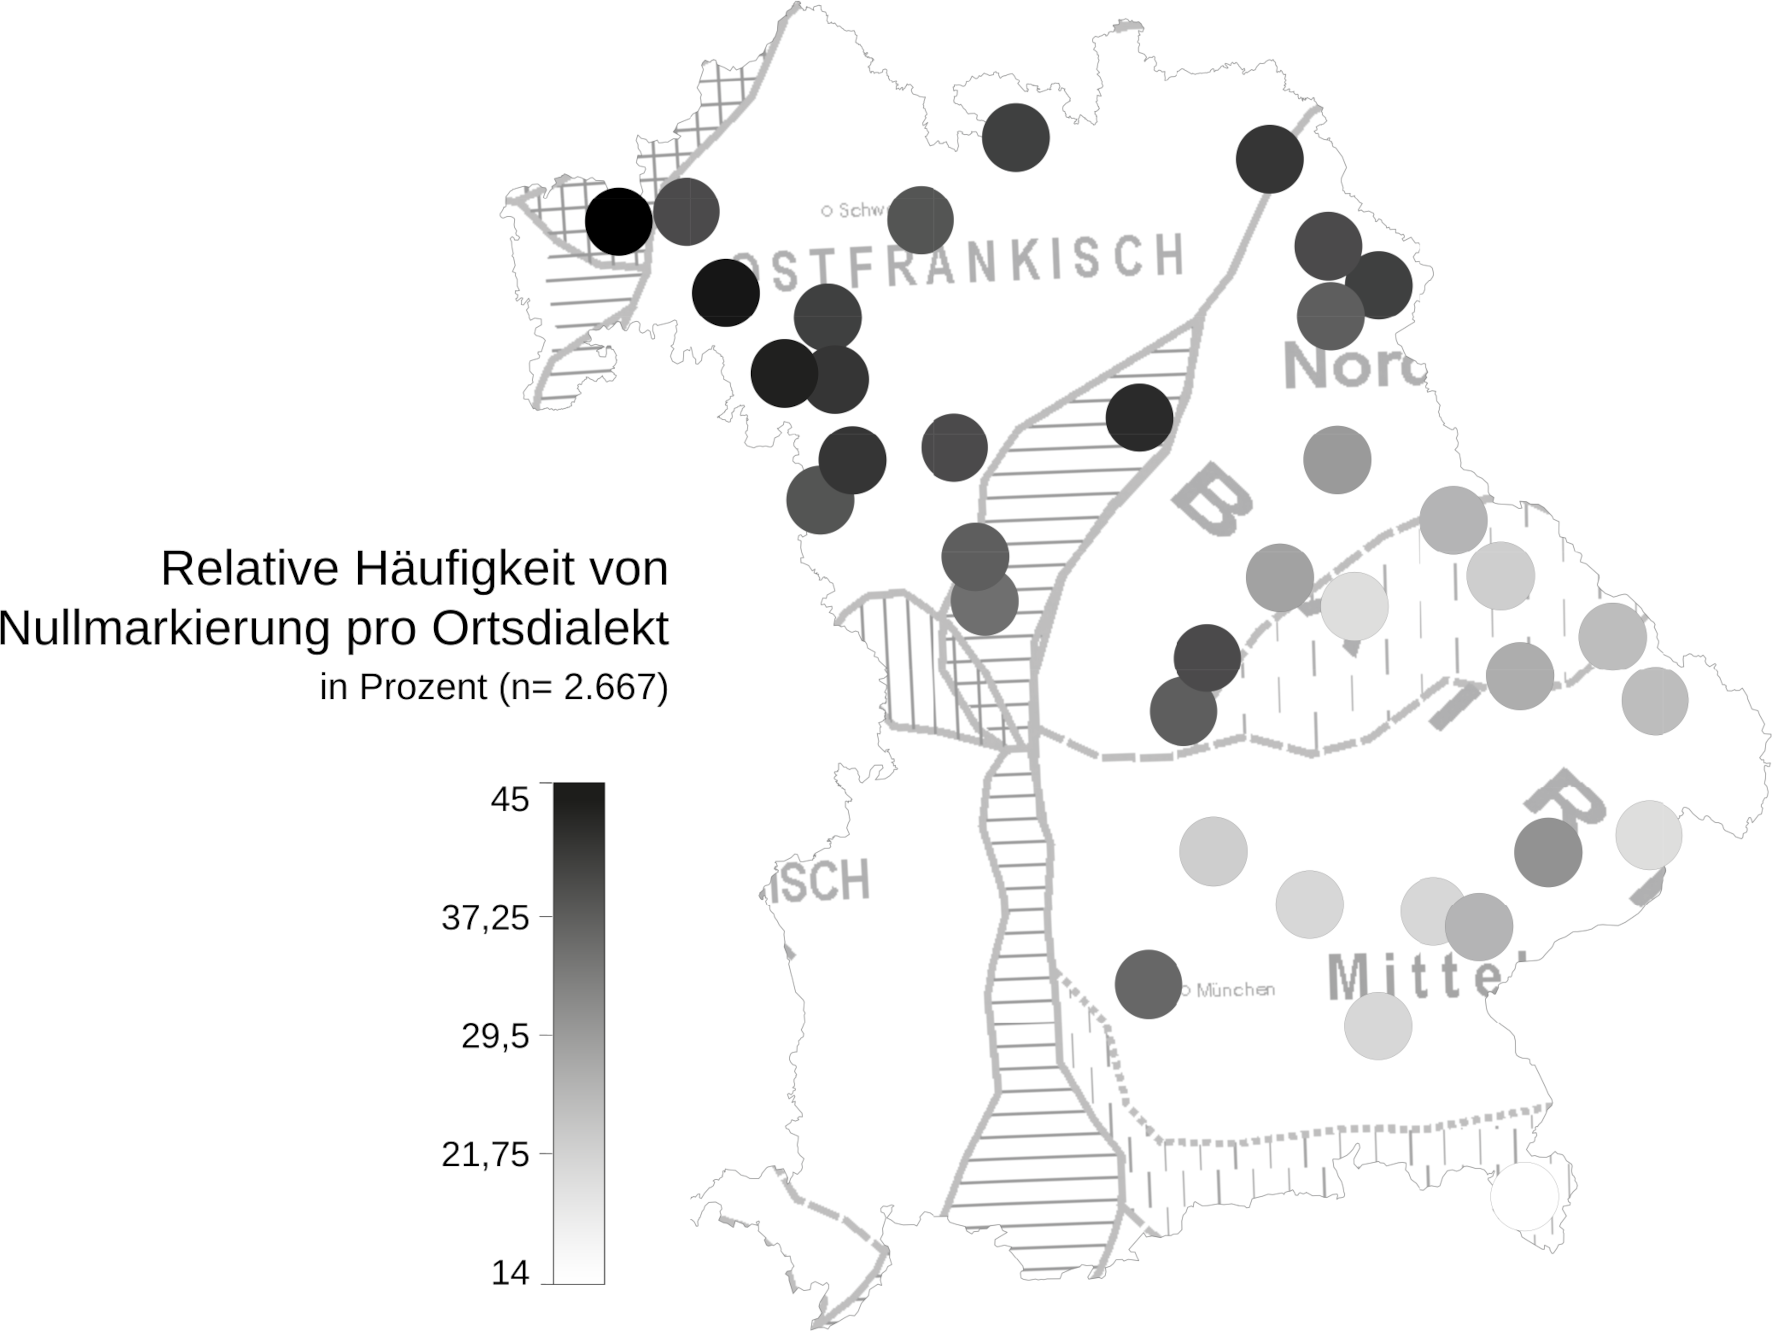
\includegraphics[width=\textwidth]{figures/Karte21.png}
\caption{Chloroplethkarte der relativen Häufigkeit von Nullmarkierung pro Ortsdialekt}
\label{map:21}
\end{map}

Aus diachroner Perspektive und mit Blick auf das historische Deklinationsklassensystem ist Nullmarkierung beispielsweise im Fall der historischen Zweisilber auf -\textit{el}, -\textit{er}, -\textit{en} entweder bereits im Mittelhochdeutschen vorhanden oder als Folge der Apokope des Schwa-Suffixes bei den historischen \textit{a}{}- und \textit{i}{}-Stämmen das Ergebnis eines phonologischen Prozesses (vgl. \sectref{sec:3.1.2}). Der interdialektale Vergleich zwischen Ramsau und (als Beispiel für Dialektsysteme mit einem höheren Anteil von Nullpluralen) dem ofr. Ahorn bestätigt exemplarisch für die mask. \textit{a}{}-Deklination und historische Zweisilber auf -\textit{el}, -\textit{en} den generellen Befund. Beide Substantivklassen weisen im ofr. Ahorn eher Numerussynkretismus auf, während Pluralformen im mittelbair.-südbair. Ramsau durch additive oder stammaffizierende Markierungsstrategien gebildet werden: \teuthoo{dê}{d{\burgereshwa}} \teuthoo{vis\#}{viš} -- \teuthoo{di}{di} \teuthoo{vis\#}{viš} ‚Fisch‘ in Ahorn vs. \teuthoo{vi“s\#5}{vīš̩} -- \teuthoo{viS'}{viʃ̌} in Ramsau, \teuthoo{dAq}{dαʔ} \teuthoo{å>Am}{{\burgerôalpha}αm} -- \teuthoo{di.}{diͅ} \teuthoo{å>Am}{{\burgerôalpha}αm} ‚Arm‘ in Ahorn vs. \teuthoo{o<Åm}{ô{\burgershwaalpha}m} -- \teuthoo{a4m}{ạm} in Ramsau, \teuthoo{A}{α} \teuthoo{ha)\$ovm@}{ha\klammeruntenpost{}̤ovm̥} -- \teuthoo{ha)\$ovm@}{ha\klammeruntenpost{}̤ovm̥} ‚Haufen‘ in Ahorn vs. \teuthoo{ha4<ofn@}{hậofn̥} -- \teuthoo{ha4<i.fn@}{hậiͅfn̥} in Ramsau, \teuthoo{s\#no<8ubl@}{šnô\klammerobenpost{}ubl̥} -- \teuthoo{s\#no<8ubl@}{šnô\klammerobenpost{}ubl̥} ‚Schnabel‘ in Ahorn vs. \teuthoo{s\#no<æi:}{šnô{\burgerbw}i{\doubleogonek}} -- \teuthoo{s\#na4<æen}{šnậ{\burgerbw}en} in Ramsau. Es handelt sich hier aber nur um Tendenzen, auch in Ahorn gibt es Belege für Deklinationsklassenwechsel der mask. \textit{a}{}-Stämme (z.\,B. \teuthoo{dÅ}{d{\burgershwaalpha}} \teuthoo{hu(+nd}{hũ\klammerobenpost{}nd} -- \teuthoo{hu6?nd}{hü̃nd} ‚Hund‘) und in Ramsau Belege für Nullplural (\teuthoo{we94<g@}{we\klammeruntenpost{}̣̂ɡ̥} -- \teuthoo{we94<g}{we\klammeruntenpost{}̣̂ɡ} ‚Weg‘).

Numerussynkretismus und stammaffizierende Markierung können somit die lautgesetzliche Entsprechung der mhd. Flexionsformen sein. In Dialekten mit Lenis-Fortis-Opposition im phonologischen System ist die Pluralvariante \teuthoo{vi“s\#5}{vīš̩} -- \teuthoo{viS'}{viʃ̌} die lautgesetzliche Form, in Dialekten ohne diese Opposition entspricht ihr hingegen die synkretische Form. Inwiefern synchrone Numerussynkretismen oder formale Numerusdifferenzierung für einzelne Substantive oder Substantivgruppen lautgesetzlich entstanden oder das Ergebnis von Deklinationsklassenwechsel sind, wird in Form einer kontrastiven Analyse des historischen und des synchronen Deklinationsklassensystems in \sectref{sec:8.2} behandelt.

\begin{sloppypar}
Daneben kann Numerussynkretismus das Ergebnis von morphologischen „Umschichtungen“ \citep[185]{Rowley1997} im Paradigma sein. Das Flexiv der obliquen Kasusformen oder der Pluralform dringt in die Form des Nom.Sg. ein, in der Folge erscheint Formensynkretismus. Im Falle mhd. schwacher Feminina sowie einiger schwacher Neutra erfolgt die Singularstammbildung durch Nasalsuffix (Typ \teuthoo{mu.gY}{muͅɡ{\klammerNG}} -- \teuthoo{mu.gY}{muͅɡ{\klammerNG}} ‚Mücke‘ im ofr. Burgbernheim, vgl. \sectref{sec:7.1.3.1}), bei einer relativ heterogenen Gruppe an Substantiven durch Umlaut (Typ \teuthoo{dA}{dα} \teuthoo{e?9.b5v5l.}{ë\klammeruntenpost{}ͅb̩v̩lͅ} -- \teuthoo{e?(9.b5v5l@}{ë\klammerobenpost{}\klammeruntenpost{}ͅb̩v̩l̥} ‚Apfel‘ im ofr. Hallerstein, vgl. \sectref{sec:7.1.3.2}).
\end{sloppypar}

\subsubsection{Singularstammbildung mit Nasalsuffix}
\label{sec:7.1.3.1}
Feminina, die synchron eine zweisilbige Struktur mit Reduktionssilbe auf Schwa aufweisen (Type \textit{Brücke}), werden in der Singularform im UG entweder mit apokopiertem Schwa realisiert (\teuthoo{bru.kx}{bruͅkx}, im mittelbair.-südbair. Ramsau) oder weisen Singularstammbildung mit Nasalsuffix auf (\teuthoo{A}{α} \teuthoo{bru?gN@}{brüɡŋ̥} im ofr. Ahorn, vgl. \cites[401]{Rowley1990a}[132--133]{Rowley1997}). Variation besteht in der formalen Realisierung des Nasalsuffixes, in Abhängigkeit vom vorausgehenden Laut wird
{}-\textit{en} zu [m] oder [ŋ] assimiliert oder vokalisch als [ɐ] realisiert (vgl. \sectref{sec:7.1.1.1}). Die \textit{n}{}-Erweiterung stellt dabei ein produktives morphologisches Verfahren der Singularstammbildung dar (z.\,B. \teuthoo{s\#a4tu<i.“4n}{šạtûị̄ͅn}, ‚Schatulle‘ im mittelbair. Neukirchen am Inn oder \textit{loɪb̥m̩} ‚Loipe‘ im Salzburger Lungau, \citealt[132]{Mauser2000}).

In der Literatur gibt es unterschiedliche Herangehensweisen hinsichtlich des Bezugssystems, vor dessen Hintergrund die Beschreibung der Singularstammbildung erfolgt. \citet[186]{Rowley1997} beispielsweise bezieht die Singularstammbildung auf die mhd. Klassen. Diese Lösung wurde mit Blick auf den diachronen Vergleich der Deklinationsklassenzugehörigkeit primär auch für diese Arbeit gewählt, wenngleich es sich um ein Bezugssystem handelt, für das mit Blick auf Pluralmarkierungsverfahren und Singularstammform bereits im Mittelhochdeutschen Variation angenommen werden muss (vgl. \citealt[3--4]{SBS9.1}). In den BSA-Bänden wurde für die nominale Flexionsmorphologie indes grundsätzlich das Neuhochdeutsche als primäres Bezugssystem herangezogen (vgl. \citealt[XXXVI]{SBS9.1}, \citealt[8]{SMF7}). Dies hat für die Singularstammform der Feminina (Apokope vs. \textit{n}{}-Erweiterung) den Vorteil, dass diese nhd. Substantivklasse formal einheitlich ist. \mapref{map:22} (Kartenbild links) zeigt für Feminina dieses Typs und das nhd. Bezugssystem die Häufigkeitsverteilung der Singularstammform im Korpus. Apokopierte und \textit{n}{}-erweiterte Stämme sind im gesamten UG zu finden, allerdings variieren die jeweiligen relativen Anteile. Die Stammbildung mit Nasalsuffix stellt das frequentere Verfahren dar, der Anteil der apokopierten Formen ist in den bair. Dialekten dabei tendenziell höher als im Ofr. Nur im mittelbair. Kirchensur und im mittelbair.-südbair. Ramsau werden die Singularformen mehrheitlich apokopiert realisiert. Gleichzeitig zeigt die Durchsicht sämtlicher Feminina mit \textit{n}{}-Erweiterung, dass diese Form der Singularstammbildung eben nicht nur nhd. zweisilbige Feminina auf Schwa umfasst, sondern ein produktives Verfahren für CVCV-Feminina insgesamt ist.


\begin{map}
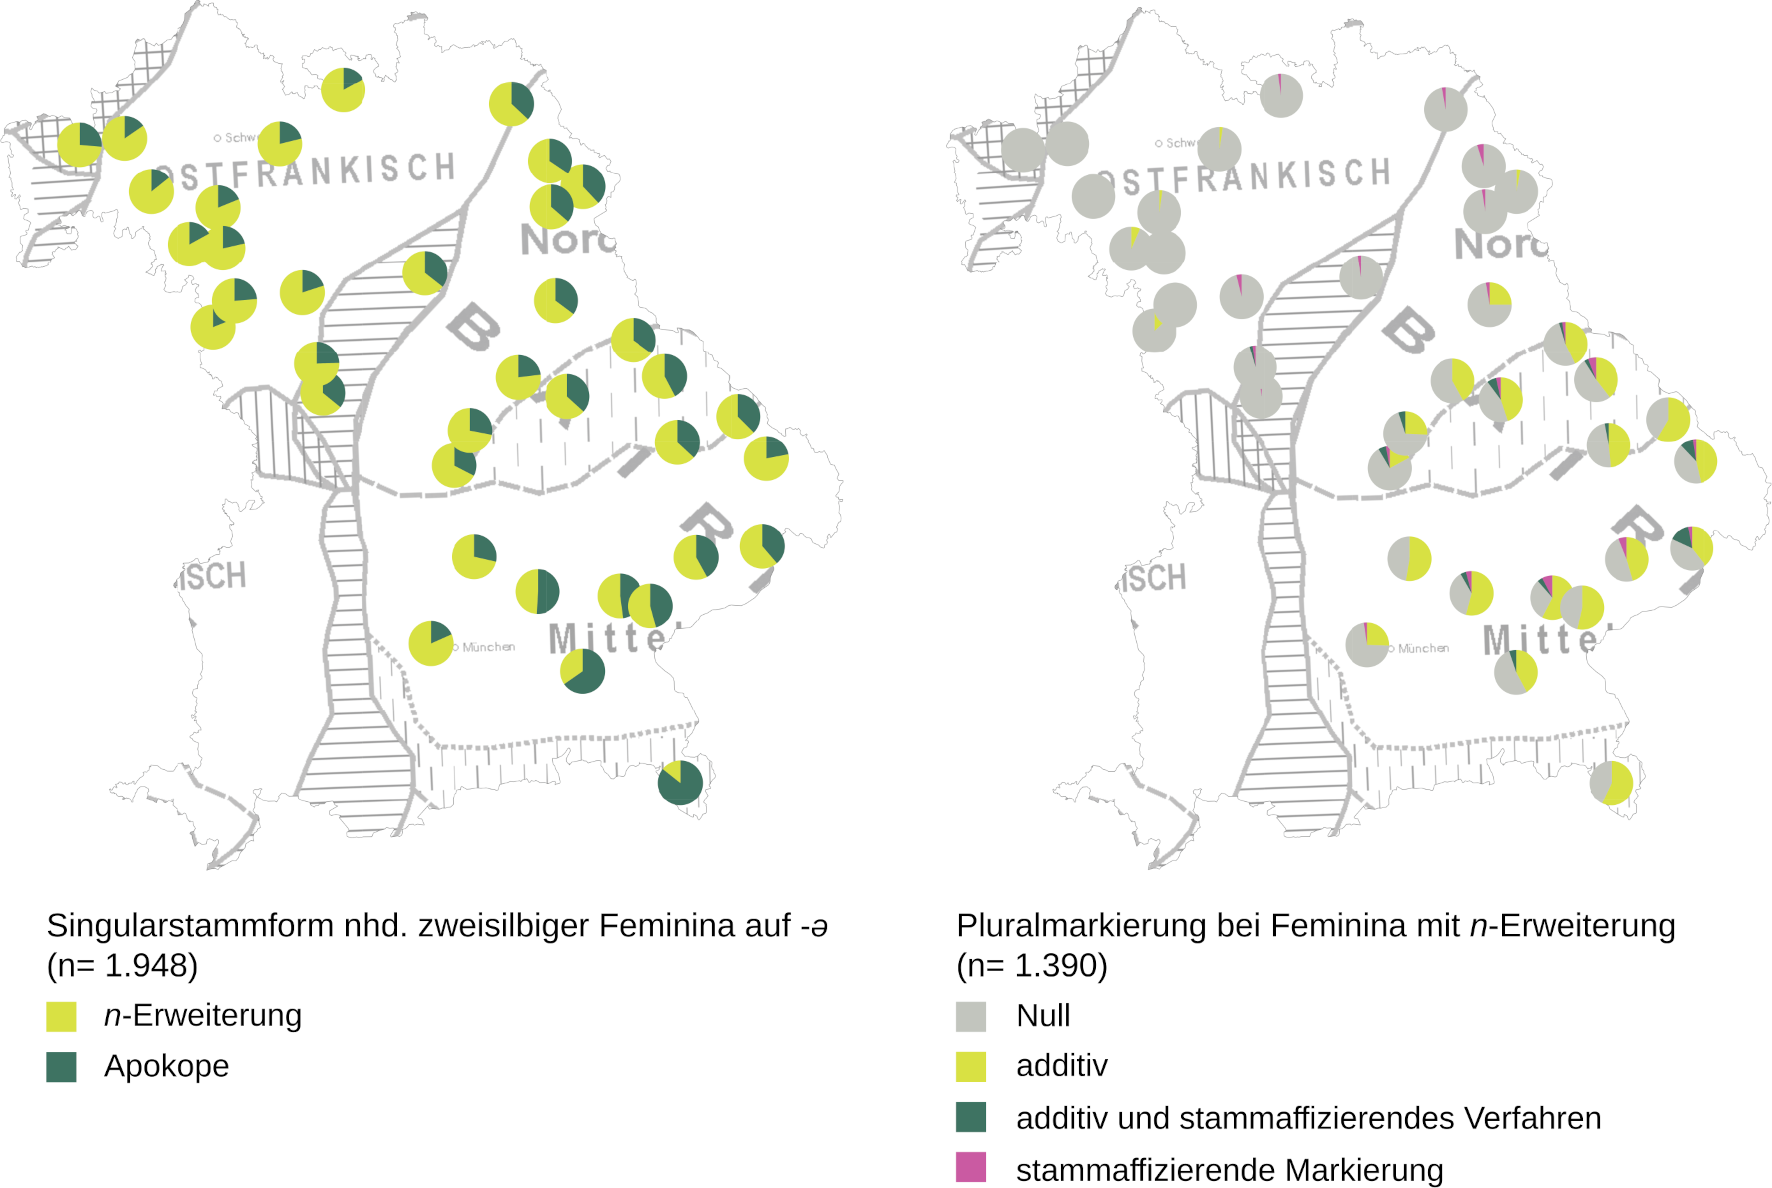
\includegraphics[width=\textwidth]{figures/Karte22.png}
\caption{Singularstammform nhd. zweisilbiger Feminina im Korpus und Häufigkeitsverteilung der Pluraltypen bei \textit{n-}erweiterten Feminina}
\label{map:22}
\end{map}

\begin{sloppypar}
Beide Stammformvarianten sind für die fem. Lexeme im Korpus belegt. Nur in wenigen Fällen findet sich ausschließlich eine der Stammformen, so wird \textit{Katze} nur apokopiert realisiert, \textit{Kette} und \textit{Latte} hingegen nur mit Nasalsuffix. Für das SBS-Arbeitsgebiet wurde die Verteilung von apokopierten vs. nicht-apokopierten Stämmen systematisch untersucht, wobei für die verschiedenen Varianten der Singularform „keine kategorisierenden Kriterien gefunden werden konnten“ (\citealt[147 und Karten 55, 62, 67]{SBS9.1}, vgl. auch \citealt[94]{Merkle1984}). Unter Berücksichtigung der historischen Klassen zeigt \citet[191--192]{Rowley1997} dagegen, dass die synchrone Formenbildung zunächst vor allem die Zugehörigkeit zur schwachen \textit{n}{}- vs. zur starken \textit{ô}{}-Deklination im Mittelhochdeutschen widerspiegelt, auf untergeordneter Ebene kommen dialektspezifisch semantische Aspekte hinzu (siehe hierzu ausführlicher \sectref{sec:8.2.3}).
\end{sloppypar}


\begin{sloppypar}
Die Darstellung der Häufigkeitsverteilung der Pluralmarkierungsstrategien bei sämtlichen \textit{n}{}-erweiterten Feminina in \mapref{map:22} (rechts) zeigt zudem, dass dialektspezifische Unterschiede hinsichtlich der Pluralform bestehen: Im Ofr. und im nördlichen Nordbair. finden sich fast ausschließlich Numerussynkretismen, während im südlichen Nordbair., im Mittelbair. sowie den bair. Übergangsgebieten additive Pluralmarkierung belegt ist und teilweise die frequentere Pluralmarkierungsstrategie darstellt. Hier lohnt es, die Form des Singularstammes neben dem Pluralmarkierungsverfahren als weiteres Merkmal der synchronen Deklinationsklassen heranzuziehen, um (1) den relativen Anteil \textit{n}{}-erweiterter Stämme am Null- bzw. am numerusdistinkten Pluralmarkierungsverfahren und (2) mögliche dialektspezifische Pluralmarkierungsstrategien für diese Struktur des Singularstammes zu ermitteln (Abschnitte~\ref{sec:8.3.1.3} und \ref{sec:8.3.3.1}).
\end{sloppypar}

Daneben findet sich die Generalisierung des Nasalsuffixes bei einigen mhd. his\-to\-risch schwachen und starken Maskulina und Neutra. Im Ofr. sind vereinzelt die Maskulina \textit{Backe,} \textit{Fleck,} \textit{Ochse} und \textit{Spatz} belegt,\footnote{\textit{Backe} und \textit{Fleck} wurden nur im SMF-Teilprojekt in der Singular- und Pluralform abgefragt.} in den bair. Dialekten finden sich die Neutra \textit{Auge}, \textit{Ohr} und das Maskulinum \textit{Hachse} (vgl. \citealt[§137]{Kollmer1987}, \citealt[8--9]{Mausser1915}, \citealt[190]{Rowley1997}, \citealt[121]{Steininger1994}, \citealt[147]{Wildfeuer2001}).

\subsubsection{Singularstammbildung mit Umlaut}
\label{sec:7.1.3.2}
Im gesamten UG (mit Ausnahme des ofr.-hess. Wiesthal, des mittelbair. Pasing und des mittelbair.-südbair. Ramsau) erscheinen die mhd. starken Feminina \textit{Bank}, \textit{Hand} und \textit{Wand} mit dem Umlaut des mhd. Pluralparadigmas bzw. der Obliquusformen des Singularparadigmas in der Nominativ-Singular-Form, z.\,B. \teuthoo{b5e.Nk\_}{b̩eͅŋkʰ} -- \teuthoo{b5e.Nk\_}{b̩eͅŋkʰ} ‚Bank‘ im nordbair. Groschlattengrün, \teuthoo{ve4nd}{vẹnd} -- \teuthoo{ve4nd}{vẹnd} ‚Wand‘ im ofr. Burgbernheim (vgl. \citealt[54]{Roth1940}, \citealt[190]{Rowley1997}, \citealt[443]{Schirmunski1962}, \citealt[§803]{Schmeller1821}).\footnote{\citet[325]{Schiepek1908} führt für das nordbair. Egerland außerdem noch die synkretischen Singular- und Pluralformen bei den Feminina \textit{Bráit} ‚Braut‘, \textit{Néit} ‚Nute‘ und \textit{Háit} ‚Haut‘ sowie \textit{Áks} (mit Umlaut) ‚Achse‘ u.a. an. Vgl. zudem die Darstellung in den Dialektgrammatiken von \citet[31]{Förster1912/13}, \citet[86]{Kemmeter1924}, \citet[285--284]{Schübel1955}.}  Da im Bair. -- laut \citet[331]{Zehetner1983} im „ländlichen Dialekt“ -- auch die Fortiskonsonanz des Plurals in den Singular eingedrungen ist, ist in den Singularformen der bair. Untersuchungsorte (nicht aber in der Diminutivform) teilweise neben Umlaut auch Fortiskonsonanz zu finden, z.\,B. \teuthoo{he.nt\_}{heͅntʰ} -- \teuthoo{he.nt\_}{heͅntʰ} --Dim. \teuthoo{he.nd5Al}{heͅnd̩αl} ‚Hand‘ im nordbair.-mittelbair. Blaibach. Im ofr.-hess./ofr.-rheinfränk. Teil des UGs, in dem subtraktive Formen belegt sind, sind die Subtraktionen der Pluralform auch in der Singularform zu finden, z.\,B. \teuthoo{hen}{hen} -- \teuthoo{di}{di} \teuthoo{hen}{hen} -- Dim. \teuthoo{henHEn}{henhͯən} ‚Hand‘ im ofr.-hess. Straßbessenbach (vgl. \citealt[12]{Hirsch1958}). Infolge des Eindringens der Pluralflexive in den Nom.Sg. weisen Singular- und Pluralformen keine Numerusdifferenzierung auf, allerdings sind großräumig \textit{Wand} und z.\,T. \textit{Bank} im Bair. und vereinzelt auch im Ofr. mit additiver Pluralmarkierung belegt, z.\,B. \teuthoo{be.Nk\_}{beͅŋkʰ} -- \teuthoo{be.NgN}{beͅŋɡŋ} ‚Bank‘ im ofr.-nordbair. Pfofeld, \teuthoo{we4nt}{wẹnt} -- \teuthoo{dwe4ntn@}{dwẹntn̥} ‚Wand‘ im nordbair. Kallmünz (vgl. \sectref{sec:8.2.3}).


\begin{map}
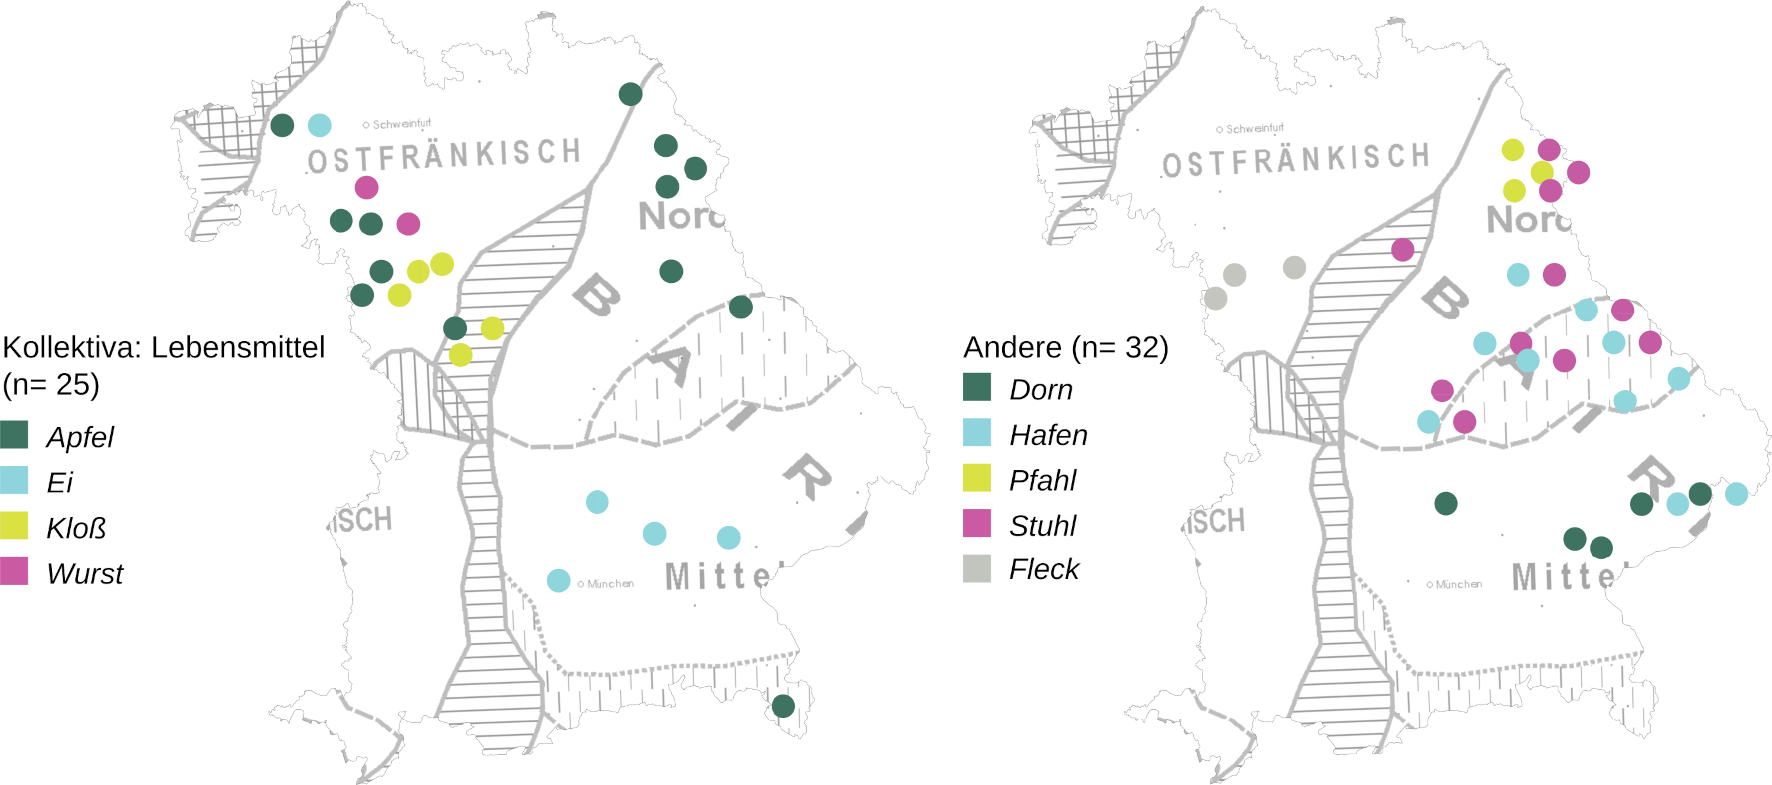
\includegraphics[width=\textwidth]{figures/Karte23.png}
\caption{Areale Verteilung von sogenannten Markiertheitsumkehrungen}
\label{map:23}
\end{map}

\citet[190]{Rowley1997} argumentiert, dass \textit{Bank}, \textit{Hand} und \textit{Wand} typischerweise in Lokativphrasen vorkommen („auf der Bank, an der Wand, in der Hand“), was zu einer „Primärspeicherung“ der Obliquusformen und in der Folge zu einer Generalisierung des Umlauts im gesamten Singularparadigma geführt haben kann (vgl. \citealt[54]{Roth1940}, \citealt[843]{Tiersma1982}). Zudem gehört \textit{Hand} zur semantischen Gruppe der paarigen Körperteile, in der auch die Neutra \textit{Auge} und \textit{Ohr} Numerussynkretismen aufweisen (vgl. \sectref{sec:8.3.2.1}). Das Vorkommen in Menge und damit die höhere Vorkommensfrequenz der Pluralform kann auch das Eindringen des Umlauts in die Singularform bei einer relativ heterogenen Gruppe an Substantiven erklären, die durch weitere Belege in Dialektgrammatiken noch ergänzt werden kann: die Lebensmittel \textit{Apfel}, \textit{Kloß}, \textit{Wurst}, daneben \textit{Dorn}, \textit{Hafen}, \textit{Pfahl} und \textit{Stuhl}\footnote{Vgl. \citet[Karte 99]{Brendel1962}.} sowie -- als Einzelbelege -- \textit{Bloch}, \textit{Darm}, \textit{Floh}, \textit{Furche}, \textit{Turm}, \textit{Zopf} (vgl. \citealt[189]{Rowley1997}, \citealt[324--325]{Schiepek1908}, \citealt[442--443]{Schirmunski1962}). \mapref{map:23} illustriert, dass die einzelnen Fälle teilweise für einzelne oder mehrere Dialekträume belegt sind, z.\,T. aber auch nur einem kleinen Gebiet vorkommen.

Ausgehend von ihrer Semantik und Gebrauchsfrequenz kann das Eindringen des Umlauts der Pluralform (im Fall von \textit{Ei} ist es das Eindringen des \textit{r}-Suffixes) in die Singularform als sogenannte Markiertheitsumkehrung im Sinne \citegen[48--58]{Mayerthaler1981} klassifiziert werden: Die Pluralform ist die frequentere und damit unmarkierte Form (ausführlicher hierzu \citealt{Bybee2010}). Wie bei den starken Feminina \textit{Wand} und \textit{Bank} finden sich auch hier neben Numerussynkretismen als Normalfall Belege für formale Numerusdifferenzierung wie die additive Markierung von \teuthoo{de.2n}{dēͅn} -- \teuthoo{de.2nA}{dēͅnα} ‚Dorn‘ im mittelbair. Wolfersdorf und \teuthoo{s\#dôe{\textasciitilde}îl}{šd{\aufstrih}e{\aufstrih}l}
 -- \teuthoo{s\#dôe{\textasciitilde}îln@}{šd{\aufstrih}e{\aufstrih}ln̥} ‚Stuhl‘ im nordbair.-mittelbair. Blaibach oder die stammaffizierende Form \teuthoo{he42vA}{hẹ̄vα} -- \teuthoo{the4vA}{thẹvα} ‚Hafen‘ im nordbair.-mittelbair. Grafenkirchen. Bemerkenswert ist hier die Form \teuthoo{dsi.“bv5}{dsīͅbv̩} (neben \teuthoo{dse\$2bv}{dsē̤bv}) ‚Zopf‘-- \teuthoo{di}{di} \teuthoo{la.NE}{laͅŋə} \teuthoo{dse4bv}{dsẹbv} ‚die langen Zöpfe‘ im ofr.-hess. Wiesthal.: Der innerparadigmatische Wechsel der Zungenhöhe zwischen \teuthoo{i.“}{īͅ} und \teuthoo{e.}{eͅ} ist historisch aus der Hebung von mhd. \textit{ö} in Dehnung in der Singularform und mhd. \textit{ö} in der Pluralform in Normalentwicklung entstanden (vgl. \sectref{sec:7.1.2.1.1}). Das Eindringen des Umlauts in die Singularform ist damit älter als die phonologischen Prozesse Einsilberdehnung und Hebung von mhd. \textit{ö}.

\subsection{Suppletion}
\label{sec:7.1.4}
Synchron ist eine Form dann suppletiv, „wenn sie nicht nach allgemeinen phonologischen oder morphologischen Regeln abgeleitet werden kann“ \citep[78]{Nübling1999}. \citet{Melcuk2000} fokussiert in seinem Überblicksartikel zur Suppletion zugleich den relationalen Charakter des Phänomens. Suppletiv ist weder eine linguistische Einheit noch eine linguistische Operation, sondern Suppletion beschreibt eine binäre Beziehung zwischen zwei sprachlichen Zeichen X und Y („X is suppletive with respect to Y“, \citealt[510]{Melcuk2000}). Im Bereich der Flexionsmorphologie wird Suppletion als „Extremfall von Irregularität“ \citep[77]{Nübling1999}, als „Störungen des grundlegenden Uniformitätsprinzips ‚eine Bedeutung -- eine Form‘“ häufig als marginales Phänomen behandelt und dargestellt. Forschung zu suppletiven Flexionsformen in der Standardsprache und zur diachronen Herausbildung suppletiver Formen in verschiedenen Sprachen zeigt indes, dass (1) Suppletion und eine hohe Gebrauchsfrequenz korrelieren und (2) suppletive Formen tendenziell kurz und komprimiert sind, was aus sprachökonomischer Perspektive einen Vorteil im Bereich der Performanz bedeutet (vgl. \citealt{Nübling1999}, \citealt{Plank1981}, \citealt{Ronneberger-Sibold1988}). Suppletion stellt dabei ein graduelles Phänomen dar (vgl. \citealt[514--515 und 517--519]{Melcuk2000}, \citealt[30]{Plank1981}, \citealt[129]{Rowley1997}). Hinsichtlich der Ähnlichkeit zwischen zwei Formen wird zwischen den Polen starke Suppletion (keine formale Ähnlichkeit) und schwache Suppletion (Teilähnlichkeiten) unterschieden.\footnote{\citet[517--518]{Melcuk2000} unterscheidet neben der Gradualität hinsichtlich der formalen Ähnlichkeit auch Gra\-dualität hinsichtlich der Regularität der semantischen Beziehung zwischen X und Y (flexivische Suppletion als semantisch stark, derivationelle Suppletion als semantisch schwach).}

Um Suppletion im Bereich der dialektalen Flexionsmorphologie adäquat erfassen und klassifizieren zu können, muss ein Aspekt fokussiert werden, der sich aus der oben genannten synchronen Minimaldefinition von Suppletion ergibt: Inwiefern kann eine über den Einzelfall hinausgehende allgemeine phonologische oder morphologische Regel formuliert werden? Als suppletiv behandelt beispielsweise \citet[129, 166]{Rowley1997} Pluralformen, die sich zwar mithilfe formaler Marker und flexivischer Prozesse beschreiben lassen, die aber mit Blick auf die Typenfrequenz Einzelfälle darstellen. Als suppletiv zu klassifizieren wären demnach isolierte Fälle von Quantitätskontrasten oder Konsonantismusalternationen (vgl. \citealt[124, 165]{Rowley1997}) respektive von Subtraktion \citep[583]{Dressler2000}; den Referenzpunkt bildet hier das jeweilige Dialektsystem. Lassen sich innerparadigmatische Alternationen hingegen „in eine stärker besetzte Modifikation“ (wie etwa den Diphthongwechsel bei mhd. \textit{ei}) einordnen, handele es sich nicht um Suppletion, sondern um ein eigenes Flexionsmuster \citep[129]{Rowley1997}. \citet[78]{Nübling1999} unterscheidet daneben suppletive Flexionsformen, bei denen ein reguläres Flexiv an die suppletive Wurzel tritt: Durch das segmentierbare Flexiv ist die gesamte Wortform „etwas weniger suppletiv“ als eine suppletive Wortform ohne Flexiv.

Insgesamt ist die Klassifikation von Suppletion damit in vielen Fällen eine Frage der Abwägung und letztlich auch der Granularität des Datenmaterials. Um festzustellen, ob eine irreguläre Pluralform tatsächlich einen isolierten Beleg darstellt und damit möglicherweise als suppletiv zu klassifizieren ist, braucht es ein ausreichend dichtes Ortsnetz und ein entsprechendes Korpus erhobener Flexionsformen. Vor dem Hintergrund der Zusammensetzung des BSA-Korpus, des interdialektalen Vergleichs der Formenbildung und der Typenfrequenz im gesamten Korpus wurden 78 Belege als suppletiv klassifiziert. Als schwächere Formen von Suppletion wurden klassifiziert:

\begin{itemize}\sloppy
\item reduzierte Formen des Lexems \textit{Gemeinde} im Singular, nicht-reduzierte Form im Plural ($n=16$), z.\,B. \teuthoo{gma42}{ɡmạ̄} -- \teuthoo{gEma4<e\$ndn@}{ɡəmậe̤ndn̥} (ofr. Burgbernheim)
\item reduzierte Formen des Kompositums \textit{Werktag} im Singular, nicht-reduzierte Form im Plural ($n=2$): \teuthoo{we94<ArE}{we\klammeruntenpost{}̣̂αrə} -- \teuthoo{weAgát;a42g}{weαɡ͈t͓͓ạ̄ɡ} (mittelbair. Neukirchen am Inn), \teuthoo{we9.<AdE}{we\klammeruntenpost{}̂ͅαdə} -- \teuthoo{we.Agt,o.g\_}{weͅαɡt͓oͅɡʰ} (mittelbair. Inning am Holz)
\item Variation in der Singular- und Pluralform zwischen den Wortstämmen \textit{Huhn} und \textit{Henne} ($n=2$, vgl. \citealt[129]{Rowley1997}): \teuthoo{he9.nA}{he\klammeruntenpost{}ͅnα} -- \teuthoo{hu§?nê}{hü̆n{\burgereshwa}} (ofr. Ahorn), \teuthoo{hena}{hena} -- \teuthoo{hi.“nEr}{hīͅnər} (ofr. Hallerstein)
\item Variation in der Singular- und Pluralform zwischen dem Simplex \textit{Breite} und der derivierten Form \textit{Breiting} ($n=2$): \teuthoo{A}{α} \teuthoo{b5ro9.2AdA2}{b̩ro\klammeruntenpost{}̄ͅαdᾱ} -- \teuthoo{b5ro9.2Adi:NA}{b̩ro\klammeruntenpost{}̄ͅαdi{\doubleogonek}ŋα} (nordbair.-mittelbair. Bernried), \teuthoo{bra42de4N}{brạ̄dẹŋ} -- \teuthoo{bra42d,E}{brạ̄d͓ə} (ofr.-hess. Wiesthal)
\item die in \sectref{sec:7.1.2.4} beschriebenen Fälle nicht-systematischer Subtraktion ($n=5$).
\end{itemize}

Starke Suppletion liegt vor, wenn die Pluralformen außerflexivisch realisiert wurden:

\begin{itemize}
\item Die Pluralform ist durch eine Wortbildung bzw. ein anderes Lexem realisiert ($n=9$), v.\,a. Frauenbezeichnungen wie \teuthoo{b5a42i.E@re\$}{b̩ạ̄iͅə̥re̤} -- \teuthoo{b5a42o4Enwa42i.BA.}{b̩ạ̄ọənwạ̄iͅ{\btilde}ᾳ} (nordbair. Groschlattengrün)\footnote{Im Nordbair. des Egerlandes weicht man \citet[320]{Schiepek1908} zufolge den Pluralformen movierter Feminina „gerne aus“, indem Komposita mit „-mädchen“ (\textit{Wéschəmài(d)lə} ‚Wäscherinnen‘) und „-weiber“ bildet, Formen wie \textit{Wéschərinnən} fänden sich „in der Stadt“.} und \teuthoo{ba<uEs\#vra.2}{bâuəšvrāͅ} -- \teuthoo{ba<u.Es\#wo.2iwE.}{bâuͅəšwōͅiwəͅ} ‚Bäuerin‘ (ofr.-hess. Wiesthal) und \teuthoo{va4<e\$b}{vậe̤b} -- \teuthoo{va4<e\$sbîi.“4l.dA}{vậe̤sb{\aufstrih}ị̄ͅlͅdα} ‚Weib‘ (ofr. Mitteleschenbach), daneben \teuthoo{sqo\$2A2}{sʔō̤ᾱ} -- \teuthoo{dqo\$2A2nwa4s\#\%l@}{dʔō̤ᾱnwạš͈l̥} ‚Ohr‘ (nordbair.-mittelbair. Bernhardswald) und \teuthoo{do.X2}{doͅꭗ̄} -- \teuthoo{da4xAra4<i:"}{dạxαrậī{\doubleogonek}} ‚Dach‘ (mittelbair. Inning am Holz), wobei die formale Ähnlichkeit zwischen Singular- und Pluralform von Fall zu Fall stärker oder schwächer ausfällt.
\item Die Pluralform ist als Diminutivform realisiert ($n=29$), z.\,B. \teuthoo{glo<s}{ɡlôs} -- \teuthoo{gla4<sl@}{ɡlậsl̥} ‚Glas‘ (mittelbair. Grafenau). Mehrfach belegt ist dieser Typ der starken Suppletion für die Lexeme \textit{Bach}, \textit{Brücke}, \textit{Draht}, \textit{Fest}, \textit{Glas}, \textit{Kalb}, \textit{Rad}.
\item Die Singularform ist als Diminutiv realisiert, die Pluralform als flektierte Form des Simplex ($n=10$), z.\,B. \teuthoo{mu.gáAl}{muͅɡ͈αl} -- \teuthoo{b5mu.gð-N@}{b̩muͅɡ̩{}͐ŋ̥} ‚Mücke‘ (nordbair.-mittelbair. Bernried).
\end{itemize}

Aufschlussreich sind hier die Fälle intra-individueller Variation und die vereinzelten Kommentare der Gewährspersonen im Datenmaterial. So hat die Gewährsperson im ofr. Burgbernheim die Pluralformen \teuthoo{v5e9.sd5\_}{v̩e\klammeruntenpost{}ͅsd̩ʰ} -- \teuthoo{v5e9.sdJi.}{v̩e\klammeruntenpost{}ͅsd{\lkreis}iͅ} neben der Form \teuthoo{v5e9.sdEr}{v̩e\klammeruntenpost{}ͅsdər} ‚Fest‘, \teuthoo{dra.2d5\_}{drāͅd̩ʰ} -- \teuthoo{dre.2dli.}{drēͅdliͅ} neben der Form \teuthoo{dre.2d5\_}{drēͅd̩ʰ} realisiert und die Diminutivformen jeweils mit „das ist die Mehrzahl“ kommentiert. Die Gewährsperson im ebenfalls ofr. Gebsattel hingegen hat die Pluralformen \teuthoo{k\_alb}{kʰalb} -- \teuthoo{k\_e.lBli.}{kʰeͅl{\btilde}liͅ} ‚Kalb‘, \teuthoo{bo.2x}{bōͅx} -- \teuthoo{be.Xli.}{beͅꭗliͅ} ‚Bach‘ gebildet und die suggerierten flektierten Simplexformen abgelehnt (vgl. \citealt[29]{SMF7}). Dass die Diminutivform damit eine reguläre, flexivische Pluralform zumindest in diesen (lexemspezifischen) Fällen ersetzen kann, legen die Gewährspersonenkommentare nahe und auch, dass es tendenziell die gleichen Substantive im Datenmaterial sind, deren Pluralform in Form eines Diminutivs gebildet werden. Interessant ist hier auch die Einschätzung im SMF: Die flexivischen Pluralformen sind „von den GPs [Gewährspersonen, GN] ganz eindeutig konstruiert und sind wohl in der entsprechenden Grundma. [Grundmundart, GN] nicht geläufig“, es bestehen „ohne Arealbildung gewisse Schwierigkeiten mit der Kategorie Plural“ (\citealt[29]{SMF7}). Suppletive Formen finden sich dabei vor allem im psychischen Nah- und „‚unmittelbaren Erfahrungsbereich‘ der Sprecher“ (\citealt[57]{Harnisch1990}, vgl. \citealt[520]{Melcuk2000}).

\section{Kasusmarkierung im UG}
\label{sec:7.2}
Dialektale Kasusmarkierung findet an der Schnittstelle von Morphologie und Syntax statt. Diachron ist die Markierung der Kasusinformation am Substantiv in den untersuchten Dialekten weitestgehend abgebaut worden, sodass die Singular- und Plural-Kasusparadigmen mehr oder weniger aus synkretischen Formen bestehen. In den Dialekten des UGs findet damit eine Entwicklung der Deflexion der Kasusinformation am Substantiv statt, die in den Dialekten des Deutschen insgesamt, aber auch für die Standardsprache belegt ist (vgl. \chapref{chap:4}). Gleichzeitig finden sich auch im Bereich der Kasusflexion dialektraumspezifische, nämlich v.\,a. nordbair. Markierungsstrategien im Dat.Pl. neben einem uniformen Nasalsuffix der obliquen Kasusformen (\sectref{sec:7.2.1}). In \sectref{sec:7.2.2} werden die verschiedenen Konstellationen von distinkten vs. synkretischen Formen im Kasusparadigma behandelt, die sich in den untersuchten Dialekten nachweisen lassen. Da dabei nicht nur die Formenbildung des Substantivs, sondern auch die der Substantivbegleiter relevant ist, wird hier immer wieder ein Vorgriff auf die Morphosyntax der Nominalphrase notwendig sein, die systematisch erst in \chapref{chap:9} dargestellt wird.\largerpage

\begin{sloppypar}
Die Auswertung der Kasusbildung erfolgt auch hier in der Word-and-par\-a\-digm-Per\-spek\-ti\-ve. Aus methodischen Gründen bilden zunächst die standardsprachlichen Abfrage-Items im Akkusativ oder Dativ des BSA-Fragebuchs den Referenzpunkt. Von den insgesamt 8.129 Singular- und Pluralformen im Nominativ sind 700 Items auch im Akkusativ und 761 Items im Dativ belegt (1.461 Kasusformen insgesamt). Für 179 Datensätze liegen sowohl Dativ- als auch Akkusativ-Items vor. Damit ist der Anteil der Substantive, für die ein Flexionsparadigma zumindest in Teilen aufgestellt werden kann, ausgesprochen gering. Zugleich variiert die Gewichtung der syntaktischen Funktionen und morphosyntaktischen Kontexte, die für die einzelnen Kasus abgefragt wurden. Erhoben wurden 29 Formen im Akk.Sg. (hiervon 11 historisch schwache Substantive\footnote{\textit{Backe}, \textit{Bauer}, \textit{Bube}, \textit{Hase}, \textit{Hecht}, \textit{Karpfen}, \textit{Ochse}, \textit{Rabe}, \textit{Spatz}, \textit{Specht} und \textit{Zecke}.} sowie 4 Präpositionalphrasen) und 8 im Akk.Pl., 14 Formen im Dat.Sg. (davon 13 Präpositionalphrasen) sowie 19 im Dat.Pl. (13 Präpositionalphrasen).\footnote{Gezählt und ausgewertet wurden hier nur jene Frage-Items, für die auch eine Nominativ-Singular- und/oder
{}-Pluralform erhoben wurde.}
\end{sloppypar}

\begin{sloppypar}
Idealiter sollte sich die Analyse der dialektalen Kasusrelationen bottom-up ausgehend von den syntaktischen Funktionen, tatsächlich realisierten Flexionsformen und der Rektion durch Präpositionen und Verben ergeben. Dies ist dann nicht möglich, wenn Kasusformen nur als isolierte Formen und ohne weiteren morphosyntaktischen Kontext erhoben oder trans\-kri\-biert wurden. In diesen Fällen erfolgt die Analyse nur top-down ausgehend vom BSA-Fragebuch, d.\,h. über die schriftsprachliche Kasusmorphologie und syntaktischen Funktionen, ggf. über die Verb\-va\-lenz. Auch hinsichtlich der formalen Variation in den Daten ist es bedauerlich, dass von den abgefragten Syntagmen bisweilen nur jene Teile trans\-kri\-biert wurden, die für den zu erhebenden Phänomenbereich relevant waren -- wenngleich dies mit Blick auf das extensive Fragebuch und die Erhebungspraxis verständlich ist.
\end{sloppypar}

Vor allem vor dem Hintergrund einer Klassifikation morphophonologischer Markierungsstrategien zeigen die Fälle von formaler Variation, die zwischen einzelnen Formen im Paradigma zu finden sind, wie schwierig die Abgrenzung von phonetisch-phonologisch bedingten (und eventuell auch freien) Alternationen und morphophonologisch funktionalisierten Alternationen ist. So bleibt offen, in welchem Umfang Sandhi-Effekte die innerparadigmatische Alternation von erhaltenem und elidiertem Konsonanten beeinflussen, z.\,B. Nom.Sg. \teuthoo{s\#do942d\_}{šdo\klammeruntenpost{}̣̄dʰ} ‚Stadt‘ -- Akk.Sg. \teuthoo{i.}{iͅ} \teuthoo{ho24}{họ̄} \teuthoo{inds,do24}{inds͓dọ̄} \teuthoo{k,E(+I(+.}{k͓ə̃\klammerobenpost{}ı̃\klammerobenpost{}ͅ} \teuthoo{mE<i.n}{mə̂iͅn} ‚ich habe in die Stadt gehen müssen‘ im nordbair. Windischeschenbach, Nom.Sg. \teuthoo{ma.+}{mãͅ} ‚Mann‘ -- Dat.Sg. \teuthoo{de+n}{dẽn} \teuthoo{oi.dn@}{oiͅdn̥} \teuthoo{ma.+n}{mãͅn} \teuthoo{ge4<m}{ɡệm} ‚dem alten Mann gegeben‘ im mittelbair. Neukirchen am Inn. Daneben besteht Variation in der Realisierung von innerparadigmatischen Kontrasten der Vokalquantität und Lenis-Fortis-Konsonanz, z.\,B. Nom.Sg. \teuthoo{d5muAt,A}{d̩muαt͓α} -- Dat.Sg. \teuthoo{da4}{dạ} \teuthoo{mu.<Ad5A}{mûͅαd̩α} \teuthoo{gðs5o9.gád\%5}{ɡ̩s̩o\klammeruntenpost{}ͅɡ͈d͈̩} ‚der Mutter gesagt‘ im nordbair. Riedenburg und Nom.Sg. \teuthoo{k\_ob5v\%}{kʰob̩v͈} -- Akk.Sg. \teuthoo{e.}{eͅ} \teuthoo{ho.d\%}{hoͅd͈} \teuthoo{s\%e-An}{s͈e{}͐αn} \teuthoo{kho24b5v\%}{khọ̄b̩v͈} \teuthoo{a.+>kho<4u.d5}{ẫͅkhộuͅd̩} ‚er hat sich den Kopf angehaut‘ im mittelbair. Neukirchen am Inn. Der Quantitätskontrast zwischen den Singularformen im Nominativ und Akkusativ bzw. Dativ stellt keine formale Markierung der Kasusinformation dar, sondern bestätigt vielmehr die Beobachtung in \sectref{sec:7.1.2.3.1}, dass Kontraste der Vokalquantität und auch Lenis/-Fortis-Kontraste innerhalb eines phonetischen Spektrums stattfinden und dass sie, zumindest teilweise, das Ergebnis von Transkriptionseffekten sein können. Aufgrund der wenigen Items, die pro Ort und pro Sprecher mehrfach oder für verschiedene Paradigmenstellen abgefragt wurden, ist keine systematische Analyse solcher Effekte und der phonetisch-phonologischen Vorkommensbedingungen möglich. Es zeigt sich aber auch hier, in welchem Maße Flexionsmorphologie, genauer: abstrakte morphophonologische Markierungsstrategien, in der konkreten phonetischen Form variiert. Im Folgenden werden Varianten dieses Typs, die sich also aus dem Vergleich der belegten Formen ergeben und keine Kasusmarkierungsstrategien repräsentieren, ausgeblendet.

\subsection{Kasusmarkierungsstrategien und Kasusmarkerinventar}\label{sec:7.2.1}
\begin{sloppypar}
Eine formale Kodierung der Kasusinformation erfolgt in den untersuchten Dialekten durch additive Markierung. Im Dativ Singular der starken Maskulina und Neutra waren historisch auch stammaffizierende Markierungen im UG zu finden, die hier das Ergebnis lautgesetzlicher Entwicklungen infolge der innerparadigmatischen Alternation von einsilbigen Nominativ- und zweisilbigen Dativformen mit Schwa-Suffix (Typ \textit{dem Kind-e}) waren und damit in denselben phonologischen Umgebungen erscheinen wie die Alternationen zwischen Singular- und Pluralformen: Kontraste der Vokalquantität (in Kombination mit Lenis-Fortis-Kontrasten), der Diphthongwechsel von mhd. \textit{ei} sowie Subtraktion. In den Dialekten mit Einsilberdehnung unterbleibt die Dehnung in der zweisilbigen Dativform auf \textit{{}-ə}, infolge der Apokope des Schwa erscheinen rein stammaffizierende Kasusformen mit innerparadigmatischer Alternation zwischen Lang- und Kurzvokal (im Bair. in Kombination mit Lenis-Fortis-Kontrasten, vgl. Abschnitte~\ref{sec:7.1.2.2} und \ref{sec:7.1.2.3.1}). \citet[§34k3]{Kranzmayer1956} führt für die „abseitigeren Landstrich[e] des Nordbair.“ sowie für den Basisdialekt im Ofr. und im Bayer- und im Böhmerwald Belege innerparadigmatischer Quantitätskontraste zwischen Nom.Sg. und Dat.Sg. an, z.\,B. Nom.Sg. \teuthoo{dI2s\#}{dı̄š} -- Dat.Sg. \teuthoo{diS'}{diʃ̌} -- Nom.Pl. \teuthoo{diS'}{diʃ̌} ‚Tisch‘. Doch bereits \citet[51]{Roth1940} gibt in seiner Dialektgrammatik zum nordbair. Egerland an, dass die jüngere Form \teuthoo{a.}{aͅ} \teuthoo{to2x}{tōx} ‚am Dach‘ (mit innerparadigmatischem Ausgleich von Vokalquantität) die ältere, lautgesetzliche Form am \teuthoo{to.c}{toͅX} ablöst.\footnote{\citet[71]{Roth1940} führt auch für die obliquen Singular-Formen von \textit{Dorf} eine Verdrängung der lautgesetzlichen Dativ-Singularform \teuthoo{am toErf}{am toərf} ‚am Dorf‘ an (diese sei vor allem „in der gefühlsbetonten Rede“ noch zu finden), allerdings sei auch die Akkusativ-Präpositionalphrase \teuthoo{afs}{afs} \teuthoo{toEf}{toəf} ‚aufs Dorf‘ belegt, wo die lautgesetzliche Kürze der Dativ-Singular- auch auf die Akkusativ-Singular-Form übertragen ist.} In den vorliegenden Daten finden sich, mit Ausnahme der Form Nom.Sg. \teuthoo{bo.2x}{bōͅx} -- Dat.Sg. \teuthoo{do.3}{dŏͅ} \teuthoo{dri“m}{drīm} \teuthoo{i“bAn}{ībαn} \teuthoo{bo4X}{bọꭗ} ‚da drüben überm Bach‘ -- Nom.Pl. \teuthoo{be.x}{beͅx} ‚Bach’ im ofr. Hallerstein, keine Belege für innerparadigmatische Quantitätskontraste der Kasusmarkierung.\footnote{Gemeint sind hier systematische Alternationen; Alternationen zwischen Kurz- und Langvokal gibt es (in beide Richtungen) häufiger, sie scheinen aber durch phonetische Variation bedingt zu sein.}  Auch \citet[94--95]{Rowley1997} findet keine Belege für ein produktives Flexionsmuster, sondern nur „relikthafte“ Belege in idiomatisierten Wendungen mit Dat.Sg., z.\,B. \teuthoo{a.}{aͅ} \teuthoo{diS'}{diʃ̌} ‚auf dem Tisch‘ vs. \teuthoo{dsweNs}{dsweŋs} \teuthoo{dean}{dean} \teuthoo{åltn}{{\burgeroalpha}ltn} \teuthoo{di2s\#}{dīš} ‚wegen dem alten Tisch‘ im nordbair. Tirschenreuth, für das sich in den vorliegenden Daten im Singular nur Formen mit innerparadigmatischem Ausgleich von Vokalquantität und Lenis-Fortis-Konsonanz finden (Nom.Sg. \teuthoo{d5i“s\#}{d̩īš} -- Dat.Sg. \teuthoo{Am}{αm} \teuthoo{di“s\#}{dīš} -- Nom.Pl. \teuthoo{diS'}{diʃ̌}).\footnote{Laut \citet[16]{Köhler1934} „wirken“ auch im unterofr. Aschenroth innerparadigmatische Quantitätskontraste im Singularparadigma nicht „nach“. Den Befund, dass innerparadigmatische Alternationen im UG als Kasusmarkierung nicht funktionalisiert (bzw. überhaupt belegt) sind, bestätigen zudem die Auswertungen des SMF (\citealt[116--117]{SMF7}, vgl. \citealt[§283]{Gebhardt1907}).}
\end{sloppypar}

Auch für die innerparadigmatische Alternation von mhd. \textit{ei} in der einsilbigen Nominativ-Singular-Form und der historisch zweisilbigen Dativ-Singular-Form im Bair. führt \citet[94--95]{Rowley1997} nur noch relikthafte Belege an, und zwar vor allem in Ortsnamen.\footnote{In den BSA-Erhebungen wurden keine Dativ-Singular-Formen der starken Maskulina und Neutra mit mhd. \textit{ei} erhoben. Bei dem abgefragten Syntagma „das Brot zu Laib(en) formen“ wurde nicht notiert, ob die Singular- oder die Pluralform realisiert wurde -- hier sind in den Orten mit umlautähnlichem Vokalwechsel jeweils Formen mit \teuthoo{o.}{oͅ}, d.\,h. mit innerparadigmatischer Alternation, belegt.} Im ofr.-hess. Wiesthal, für das subtraktive Pluralformen nachgewiesen wurden, wird der Dat.Sg. von \textit{Hand} nicht durch Subtraktion gebildet, wenngleich hier historisch dieselben phonologischen Voraussetzungen bestanden haben: Nom.Sg. \teuthoo{ha."+nd5\_}{hã̄ͅnd̩ʰ} -- Dat.Sg. \teuthoo{e.E}{eͅə} \teuthoo{s\#yo.<i.bd}{š⅄ôͅiͅbd} \teuthoo{a.lEs5}{aͅləs̩} \teuthoo{me\$dE}{me̤də} \teuthoo{leNgá\_}{leŋɡ͈ʰ} \teuthoo{ha:2nd5\_}{ha{\doubleogonek}̄nd̩ʰ} ‚er schreibt alles mit der linken Hand‘ (vgl. \sectref{sec:7.1.2.4}). \citet[63--65]{Birkenes2014} zeigt in seiner Studie, dass subtraktive Dative für das /nd/-Konsonantencluster bereits um 1900 relativ selten waren (und vor allem in idiomatisierten Wendungen erhalten sind) und dass hier innerparadigmatischer Ausgleich zugunsten der Nominativform stattgefunden haben dürfte. Ein Blick jenseits des oobd. Dialektraums zeigt indes, dass der innerparadigmatische Ausgleich auch zugunsten der subtraktiven Form verlaufen kann, so finden sich beispielsweise im rheinfränk. Großostheim die Formen Nom.Sg. \teuthoo{di}{di} \teuthoo{he.n}{heͅn} -- Dat.Sg. \teuthoo{midE}{midə} \teuthoo{liNgð\_}{liŋɡ̩ʰ} \teuthoo{he9.n}{he\klammeruntenpost{}ͅn} -- Nom.Pl. \teuthoo{he.n}{heͅn}. Infolge der Markiertheitsumkehrung im Nom.Sg. erscheinen hier synkretische Formen im Singular und im Plural. Haben innerparadigmatische Ausgleichsprozesse bezüglich Vokalquantität, -qualität oder subtraktive Formen nur im Singularparadigma stattgefunden, besteht der Synkretismus nur im Singularparadigma, die Pluralformen sind durch Erhalt der stammaffizierenden Markierung distinkt.

Die einzigen innerparadigmatischen Alternationen, die innerhalb des Pluralparadigmas auch synchron in den Dialekten des UGs belegt sind, betreffen nach \citet[143]{Rowley1997} eine geschlossene Lexemgruppe im Ofr.: \textit{Bein}, \textit{Stein}, \textit{Pferd}, \textit{Schuh}, \textit{Zahn}. Die Dativ-Plural-Formen weisen hier jeweils einen Kurzvokal auf, die Nominativ-Plural-Formen hingegen Langvokal: Nom.Pl. \teuthoo{dse2}{dsē} -- Dat.Pl. \teuthoo{dsena}{dsena} im ofr. Stadtsteinach (Typ (b1) in 	\tabref{tab:23}). In den vorliegenden Daten finden sich zwar auch Alternationen dieses Musters (und zwar im Ofr. und im Bair., n= 8), allerdings betreffen diese andere als die genannten Lexeme, sodass von keiner morphophonologisch relevanten Alternation ausgegangen wird, z.\,B. Nom.Sg. \teuthoo{A}{α} \teuthoo{ghi“Adn@}{ɡhīαdn̥} -- Nom.Pl. \teuthoo{ghi“Adn@}{ɡhīαdn̥} -- Dat.Pl. \teuthoo{mid}{mid} \teuthoo{ghedn@}{ɡhedn̥} ‚mit Ketten‘ (mit lautgesetzlich ausgebliebener Hebung des Kurzvokals) im ofr. Ahorn, Nom.Sg. \teuthoo{dE}{də} \teuthoo{la.N}{laͅŋ} \teuthoo{o<.sd5@}{ôͅsd̩̥} -- Nom.Pl. \teuthoo{dE}{də} \teuthoo{la.NA}{laͅŋα} \teuthoo{e<s5d5}{ês̩d̩} -- Dat.Pl. \teuthoo{A}{α} \teuthoo{de4}{dẹ} \teuthoo{\_e4s\%t,\_}{ʰẹs͈t͓ʰ} ‚Ast‘ im mittelbair. Neukirchen am Inn.

\begin{sloppypar}
Da in den apokopierenden Dialekten des UGs das Schwa-Suffix nicht erhalten ist, erscheinen die starken Maskulina und Neutra ohne formale Markierung im Dat.Sg. im rezenten Dialekt (vgl. \citealt[45]{Mausser1915}, \citealt[437]{Schirmunski1962}, \citealt[§221]{Schmeller1821}).\footnote{Jenseits einzeltextabhängiger Befunde geben \citet[91]{KleinEtAl2018} bereits für das 14. Jahrhundert an, dass Texte im Bair. und im bair.-alem. Übergangsgebiet zu 100\,\% Apokope des Schwa-Suffixes im Dat.Sg. aufweisen.} Eine distinkte Form des Dat.Sg. findet sich in Form additiver Markierung mit Nasalsuffix teilweise bei den mhd. schwachen Substantiven, z.\,B. Nom.Sg. \teuthoo{he.EtS}{heͅətʃ} -- Dat.Sg. \teuthoo{a.m}{aͅm} \teuthoo{he.EtSn@}{heͅətʃn̥} -- Nom.Pl. \teuthoo{he.EtSn@}{heͅətʃn̥} ‚Herz‘ im nordbair.-mittelbair. Grafenkirchen, Nom.Sg. \teuthoo{kha.mEr}{khaͅmər} -- Dat.Sg. \teuthoo{mi.“4E}{mị̄ͅə} \teuthoo{se4n}{sẹn} \teuthoo{i.n}{iͅn} \teuthoo{dE}{də} \linebreak\teuthoo{kha):mEn}{kha\klammeruntenpost{}{\doubleogonek}mən} ‚wir sind in der Kammer‘ -- Nom.Pl. \teuthoo{kha9.mEn}{kha\klammeruntenpost{}ͅmən} ‚Kammer‘ im ofr. Krum (siehe \sectref{sec:7.2.2} zu den Paradigmenkonstellationen, vgl. \citealt[440]{Schirmunski1962}, \citealt{WA}-Karte 477 „Herzen“). Bemerkenswert ist hier das starke Maskulinum \textit{Baum} mit Nasalsuffix im nordbair. Windischeschenbach: Nom.Sg. \teuthoo{ba4m}{bạm} -- Dat.Sg. \teuthoo{a.m}{aͅm} \teuthoo{ba4<mEn}{bậmən} ‚am Baum‘ -- Nom.Pl. \teuthoo{ba<\$i.m}{bâ̤iͅm}. In den mittelbair. Dialekten (inklusive Übergangsgebiete) erscheint auch \textit{Mutter} mit dem Flexiv der schwachen Flexion (z.\,B. Nom.Sg. \teuthoo{bmuAtA}{bmuαtα} -- Dat.Sg. \teuthoo{e.}{eͅ} \teuthoo{ho.s}{hoͅs} \teuthoo{dA}{dα} \teuthoo{muAtAn}{muαtαn} \teuthoo{ksa.gðd5}{ksaͅɡ̩d̩} ‚er hat es der Mutter gesagt‘ -- Nom.Pl. \teuthoo{muAdAnA}{muαdαnα} im nordbair.-mittelbair. Blaibach).
\end{sloppypar}

Nasalsuffix findet sich im Singular auch in der Markierung der obliquen Kasus mhd. schwacher Maskulina (Typ Nom.Sg. \teuthoo{ho.s}{hoͅs} -- Akk.Sg. \teuthoo{ho2sn}{hōsn} -- Nom.Pl. \teuthoo{ho2sn}{hōsn} ‚Hase‘, vgl. \citealt[117]{SMF7}, \citealt[37]{Steinbruckner1976}).\footnote{Die folgende Darstellung bezieht sich jeweils nur auf die Akkusativ-Singular-Form, da nur diese, nicht aber Dat.Sg. erhoben wurde (vgl. hierzu die Paradigmenkonstellationen in \sectref{sec:6.2.2}).} Im westlichen Ofr. und im Unterofr. wird das Flexionssuffix im Akk.Sg. vokalisch als Schwa oder Tiefschwa realisiert, z.\,B. Nom.Sg. \teuthoo{ha.2s5}{hāͅs̩}-- Akk.Sg. An \teuthoo{ha2.sA}{hāͅsα} -- Nom.Pl. \teuthoo{ha:2sA}{ha{\doubleogonek}̄sα} ‚Hase‘ im ofr. Erlabrunn (vgl. \sectref{sec:7.1.1.1}, \citealt[Karte 42]{SUF3}). Aus systematischer sowie dialektgeografischer Sicht ist interessant, dass das Erscheinen des Nasalsuffixes morphophonologisch bedingt sein kann. In Teilen des Nordbair. und in den un\-ter\-ofr. Dialekten wird die Reduktionssilbe mhd. -\textit{en} der Singularform von \textit{Karpfen} im Nom./Akk.Sg. gleichermaßen vokalisch realisiert, doch nur im nordbair. Kallmünz wird die Akkusativ-Singular-Form mit Nasalsuffix markiert, sodass eine Art Doppelsuffigierung entsteht: Nom.Sg. \teuthoo{k,\_a.rpfA}{k͓ʰaͅrpfα} -- Akk.Sg. \teuthoo{An}{αn} \teuthoo{k,\_a.rpfAn}{kʰaͅrpfαn} -- Nom.Pl. \teuthoo{k\_arpfAn}{kʰarpfαn}. Im Unterofr. erscheinen synkretische Akkusativformen, z.\,B. im ofr. Ochsenfurt Nom./Akk.Sg. \teuthoo{ka4rb5v5E}{kạrb̩v̩ə} -- Nom.Pl. \teuthoo{ka4rb5v5E}{kạrb̩v̩ə}. Im nordbair.-mittelbair. Grafenkirchen erscheint die Doppelsuffigierung nur in der Pluralform: Nom.Sg. \teuthoo{k,\_a4p,f,A}{k͓ʰạp͓f͓α} -- Akk.Sg. \mbox{\teuthoo{k,\_a4pfA}{k͓ʰạpfα}} -- Nom.Pl. \teuthoo{k,\_a4p,f,An}{k͓ʰạp͓f͓αn}. Dass im Falle des mhd. schwachen \textit{Karpfen} im Nordbair. eine formal distinkte Form im Akk.Sg. und/""oder Nom.Pl. zur Verfügung steht, ist durch das spezifisch bair. Markierungsmuster bei Reduktionssilbe -\textit{α} und Nasalsuffix begründet (vgl. \sectref{sec:7.1.1.3}). Inwiefern es Präferenzen hinsichtlich der Paradigmenkonstellation in den bair. Dialekten gibt (Synkretismus im Singular/distinkte Pluralform in Grafenkirchen, distinkte No\-mi\-na\-tiv-Sin\-gu\-lar-Form\slash Synkretismus im Akk.Sg. und Nom.Pl.\footnote{Diese Konstellation für \textit{Karpfen} findet sich auch im nordbair. Windischeschenbach bei apokopiertem Singularstamm: Nom.Sg. \teuthoo{g\_arpf}{ɡʰarpf} -- Akk.Sg. \teuthoo{g\_arpfm@}{ɡʰarpfm̥} -- Nom.Pl. \teuthoo{g\_arpfm@}{ɡʰarpfm̥}.} in Kallmünz), muss mit Blick auf die wenigen Belege offenbleiben (siehe auch \sectref{sec:7.2.2}).

Ebenso offenbleiben muss, inwiefern die Singularstammbildung (Apokope vs. \textit{n}{}-Erweiterung) der mhd. schwachen Feminina bzw. nhd. zweisilbigen Feminina auf Schwa eine formale Markierung im Akk.Sg. bedingen kann. So finden sich im mittelbair. Reischach die Formen Nom.Sg. \teuthoo{o.<Ax}{ôͅαx} -- Akk.Sg. \teuthoo{a4<o4v5}{ậọv̩} \teuthoo{do.<AxAn}{dôͅαxαn} \teuthoo{a4<o4<v5e4}{ậộv̩ẹ} \teuthoo{gás\#5di.“4N}{ɡ͈š̩dị̄ͅŋ} ‚auf die Eiche aufhin gestiegen‘-- Dat.Sg. \teuthoo{unt,A}{unt͓α} \teuthoo{dA}{dα} \teuthoo{o.<AX}{ôͅαꭗ} -- Nom.Pl. \teuthoo{o.<AxAn}{ôͅαxαn} ‚Eiche‘. Im nordbair.-mittelbair. Grafenkirchen ist das Nasalsuffix der \textit{n}{}-Erweiterung von \textit{Eiche} vokalisch realisiert, sodass sich auch bei den Feminina die Frage stellt, in welchem Umfang Akk.Sg. bei Singularstämmen dieses Musters formal markiert wird: Nom.Sg. \teuthoo{o.ic1A}{oͅiX\⚬α} -- Akk.Sg. \teuthoo{a4<v}{ậv} \teuthoo{dqo.iX!An}{dʔoͅiꭖαn} \teuthoo{a4fi:}{ạf‌i{\doubleogonek}} \teuthoo{gra4kl@d}{ɡrạkl̥d} -- Nom.Pl. \teuthoo{o.ic1An}{oͅiX\⚬αn} (vgl. \sectref{sec:6.2.2}).

Die formale Markierung des Dativ Plural am Substantiv ist im größten Teil der untersuchten Ortsdialekte abgebaut (\mapref{map:24}, vgl. \citealt[Karte 24]{SMF7}). In jenen Dialekten, in denen im Dat.Pl. distinkte Formen belegt sind, finden sich -- zumindest teilweise -- dialektraumspezifische Markierungsstrategien oder eine dialektraumspezifische Distribution der Allomorphe (vgl. \citealt[139--143 und Karten 26, 35]{Rowley1997}).

\vfill
\begin{map}[H]
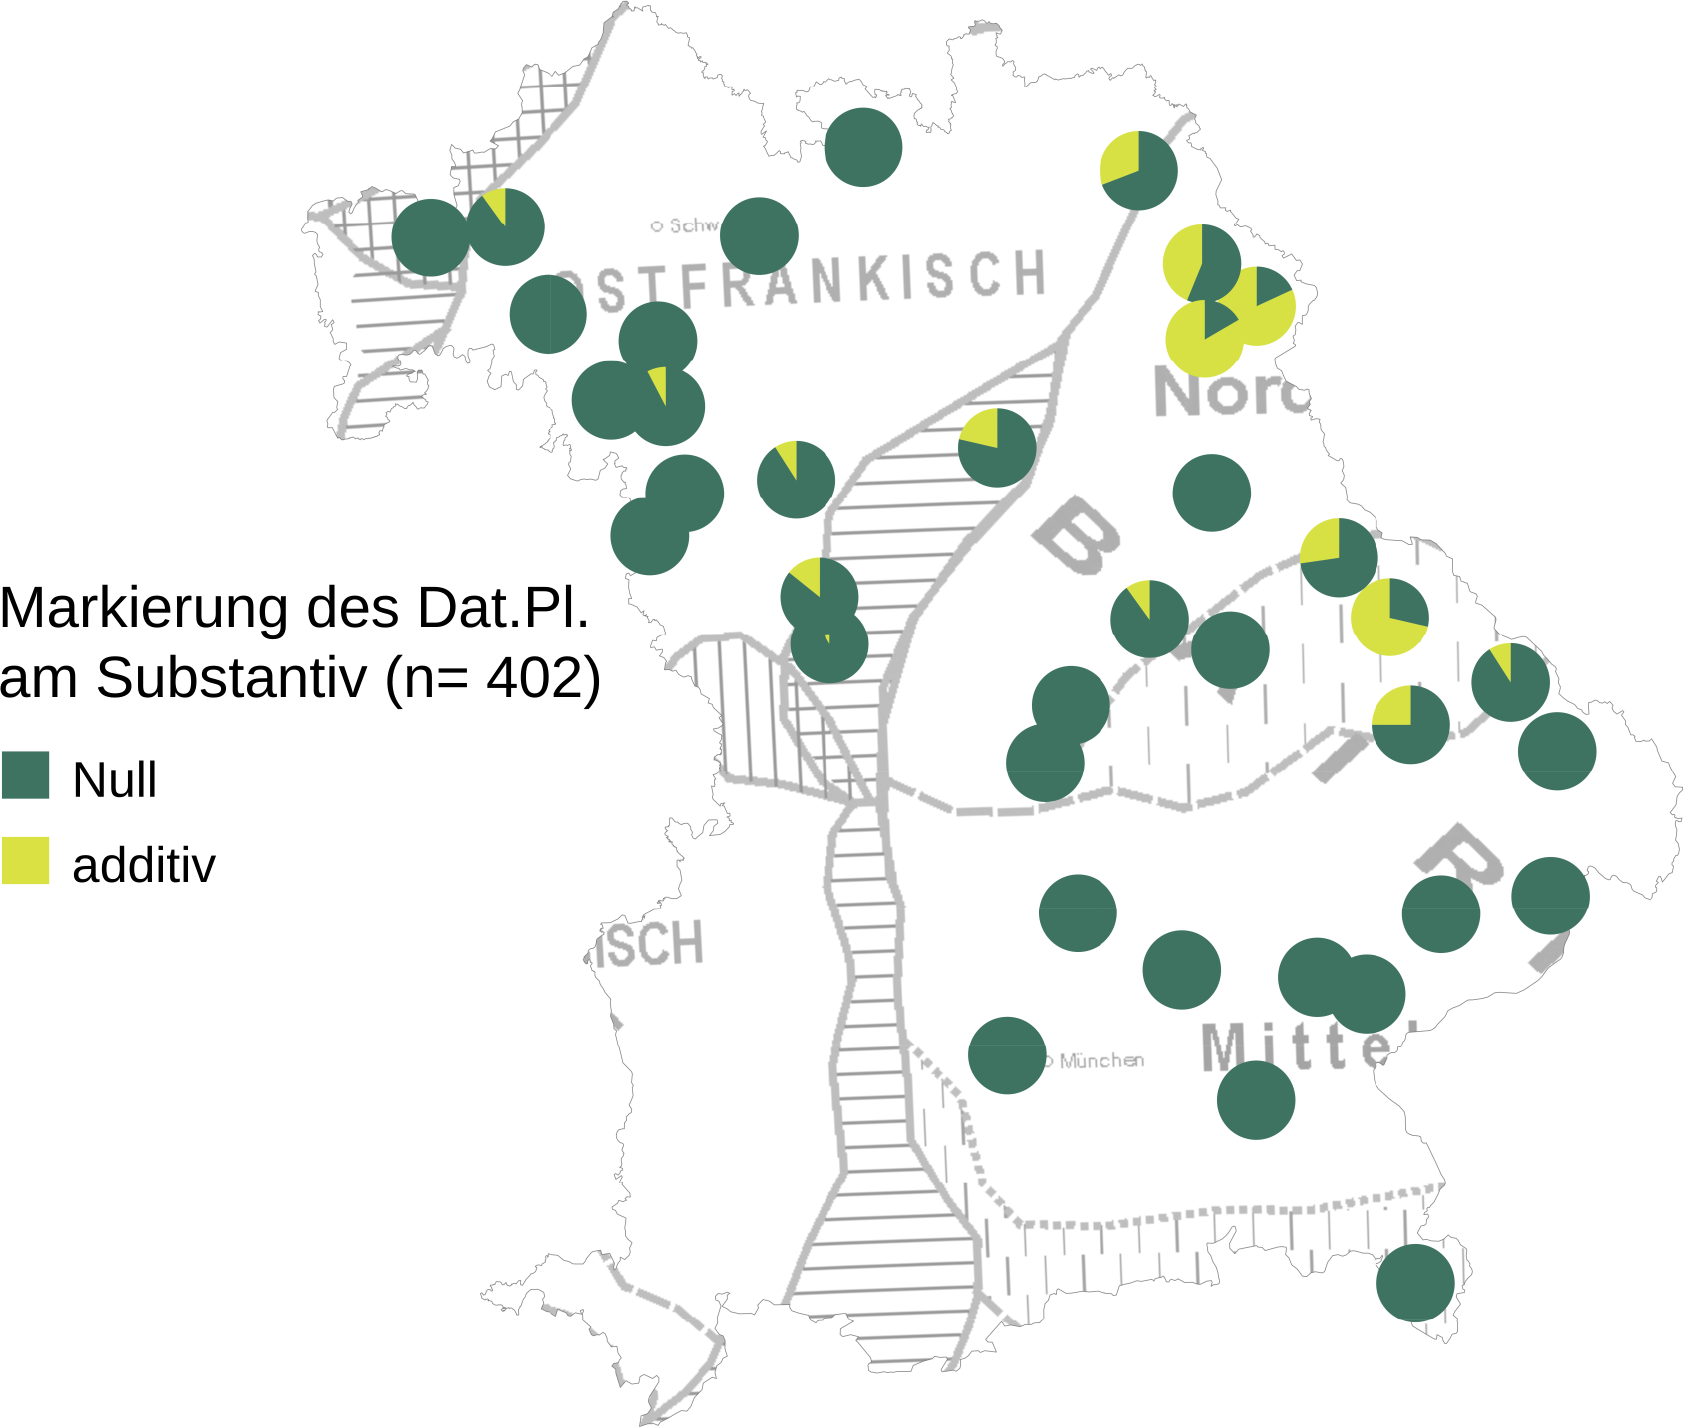
\includegraphics[width=.75\textwidth]{figures/Karte24.png}
\caption{Distinkte und synkretische Formen des Dat.Pl.}
\label{map:24}
\end{map}
\vfill\pagebreak

Im östlichen Ofr. (Tiefenbohrungspunkt Hallerstein) markiert das Suffix -\textit{na} den Dat.Pl. (bei Nasal im Auslaut des Nom.Pl. erscheint -\textit{α}, vgl. \citealt[139]{Rowley1997}): Nom.Pl. \teuthoo{k\_i“}{kʰī} -- Dat.Pl. \teuthoo{na}{na} \teuthoo{k\_ina}{kʰina} ‚Kühe‘, Nom.Pl. \teuthoo{ma942dla94}{ma\klammeruntenpost{}̣̄dla\klammeruntenpost{}̣} -- Dat.Pl. \teuthoo{den}{den} \teuthoo{glan}{ɡlan} \teuthoo{ma2dlana}{mādlana} ‚Mädchen‘, Nom.Pl. \teuthoo{di}{di} \teuthoo{k\_inEr}{kʰinər} -- Dat.Pl. \teuthoo{wel.An}{welͅαn} \teuthoo{k\_inana}{kʰinana} \teuthoo{ho.s}{hoͅs} \teuthoo{dus}{dus} \teuthoo{ge42m}{ɡẹ̄m} ‚welchen Kindern hast du es gegeben‘.\footnote{\citet[139]{Rowley1997} ebenso wie \citet[177]{Hermann1957} führen die Dativ-Plural-Form mit \textit{na}{}-Suffix auch für den Coburger Dialekt an, im Tiefenbohrungspunkt Ahorn finden sich indes nur synkretische Formen. Daneben gibt es Belege für Dativ-Plural-Formen mit \textit{na}{}-Suffix in historischen Dialektgrammatiken für das Ofr. Nürnbergs und Bambergs sowie das nördliche Nordbair. in Selb \textrm{(vgl. \citealt[§11]{Frommann1857}, \citealt[322--323]{Franke1895}, \citealt[262]{Schübel1955}, \citealt[32]{Vogt1930}).}} Von diesem dialektspezifischen Markierungstyp unterscheiden sich die nordbair. Dialekte systematisch, da hier einerseits die Form des Dativ-Plural-Markers variiert (distinkte Dativ-Plural-Formen enden auf Nasal, vgl. \citealt[139]{Rowley1997}) und es variiert -- zumindest im südlichen Nordbair. -- die präferierte Silbenstruktur: Auf die Stammsilbe können niemals zwei Reduktionssilben (Typ \teuthoo{ma2dlana}{mādlana}) folgen, sodass nach Nominativ-Plural-Formen mit den Reduktionssilben -\textit{α} und -\textit{el} ausschließlich das unsilbische Suffix \textit{{}-n} erscheint (\citealt[§147.2a]{Kollmer1987}, \citealt[140]{Rowley1997}).\footnote{Grundsätzlich ist es mit Blick auf die geringen Belegzahlen von distinkten Dativ-Plural-Formen pro Ortsdialekt schwierig, Aussagen über die Arealität der Verteilung zu treffen, es handelt sich allenfalls um Tendenzen. Erschwerend kommt hinzu, dass im bair. Teil, d.\,h. in den Teilprojekten SOB und SNiB weniger Dativ-Plural-Items abgefragt wurden als in den übrigen Projekten.} Dass diese Präferenz der Silbenstruktur auch innerhalb des Nordbair. variiert, zeigen \citegen[141]{Rowley1997} Belege aus dem nördlichen Nordbair.: Dat.Pl. \teuthoo{a4kanan}{ạkanan} ‚Äckern‘ (nordbair. Tirschenreuth), Dat.Pl. \teuthoo{autonan}{autonan} ‚Autos‘ (nordbair. Arzberg).\largerpage[2]

Ein weiterer systematischer Unterschied besteht innerhalb des Nordbair. hinsichtlich synkretischer vs. distinkter Dativ-Plural-Formen nach Reduktionssilbe -\textit{en}. Im mittleren und südlichen Nordbair. bilden Nominativ-Plural-Formen auf -\textit{en} keine distinkte Dativ-Plural-Form (z.\,B. im nordbair.-mittelbair. Blaibach Nom.Pl. \teuthoo{unsAne4}{unsαnẹ} \teuthoo{k\_a9.tSn@}{kʰa\klammeruntenpost{}ͅtʃn̥} -- Dat.Pl. \teuthoo{mid}{mid} \teuthoo{unsene4}{unsenẹ} \teuthoo{kha).tSn@}{kha\klammeruntenpost{}ͅtʃn̥} ‚mit unseren Katzen‘, vgl. \citealt[87]{Bachmann2000}, \citealt[§147.2b]{Kollmer1987}, \citealt[140]{Rowley1997}). Im nördlichen Nordbair. ersetzt das Dativ-Plural-Suffix {}-\textit{αn} das Nasalsuffix -\textit{n} der Nominativ-Plural-Form bei mhd. schwachen Feminina und Maskulina sowie bei zweisilbigen Maskulina mit Reduktionssilbe -\textit{en}: Nom.Pl. \teuthoo{unE}{unə} \teuthoo{g\_åtSn@}{ɡʰ{\burgeroalpha}tʃn̥} -- Dat.Pl. \teuthoo{mid}{mid} \teuthoo{unEn}{unən} \teuthoo{g\_åtSAn@}{ɡʰ{\burgeroalpha}tʃαn̥} ‚Katzen‘ (Groschlattengrün), Nom.Pl. \teuthoo{khi“En}{khīən} -- Dat.Pl. \teuthoo{midn@}{midn̥} \teuthoo{k\_ôe.ikhi“EdAn}{kʰ{\aufstrih}eͅikhīədαn} ‚mit den Kuhketten‘ (Tirschenreuth), Nom.Pl. \teuthoo{bôo<u.m}{b{\aufstrih}ôuͅm} -- Dat.Pl. \teuthoo{min}{min} \teuthoo{b5ôo>?(?u.BAn}{b̩{\aufstrih}ö̂̈\klammerobenpost{}uͅ{\btilde}αn} ‚mit den Buben‘ (Windischeschenbach, vgl. \citealt[20]{Micko1933}, \citealt[142]{Rowley1997}, \citealt[§574]{Schmeller1821}). \citet[174]{Schnabel2000} führt diese Form der Suffixalternation auch für das ofr. Weingarts an, wenngleich diese Form der Formenbildung „zurückgedrängt“ werde, z.\,B. Nom./
Akk.Pl. \teuthoo{xo2sn}{xōsn} -- Dat.Pl. \teuthoo{xo2se.n}{xōseͅn} ‚Hase‘. Wie auch im Bereich der additiven Pluralmarkierung stellt die Suffixalternation hier einen Grenzfall des additiven Verfahrens dar (ausführlicher hierzu \sectref{sec:7.1.1.4}).

Im nördlichen Nordbair. (Tiefenbohrungspunkte Groschlattengrün, Tirschenreuth, Windischeschenbach) weisen distinkte Dativ-Plural-Formen eine (mindestens) zweisilbige Outputstruktur mit Reduktionssilbe -\textit{αn} auf, die durch die Addition unsilbischer und silbischer Kasussuffixe bzw. durch Suffixalternation gebildet wird:

\begin{itemize}
\item {}-\textbf{\textit{n}} nach der Reduktionssilbe -\textit{α} im Nom.Pl.: Nom.Pl. \teuthoo{mo<i.d49ýA}{môiͅḍ\klammeruntenpost{}ɫα} -- Dat.Pl. \teuthoo{deAn}{deαn} \teuthoo{glo+i.6n}{ɡlõĩͅn} \teuthoo{mo<8i.d49lAn}{mô\klammerobenpost{}iͅḍ\klammeruntenpost{}lαn} \teuthoo{ge4<m}{ɡệm} ‚den kleinen Mädchen gegeben‘ (nordbair. Windischeschenbach), Nom.Pl. \teuthoo{ta4rmA}{tạrmα} -- Dat.Pl. \teuthoo{i.}{iͅ} \teuthoo{t,a4rmAn}{t͓ạrmαn} ‚in den Därmen‘ (nordbair. Tirschenreuth)
\item {}-\textbf{\textit{αn}} bei einsilbigen Pluralformen oder nach Reduktionssilbe -\textit{el}: Nom.Pl. \teuthoo{the94nt\_}{the\klammeruntenpost{}̣ntʰ} -- Dat.Pl. \teuthoo{ån}{{\burgeroalpha}n} \teuthoo{hentAn}{hentαn} ‚an den Händen‘ (nordbair. Windischeschenbach), Nom.Pl. \teuthoo{gð\_E<i.}{ɡ̩ʰə̂iͅ} -- Dat.Pl. \teuthoo{unEn}{unən} \teuthoo{g\_E<i.En}{ɡʰə̂iͅən} ‚unseren Kühen‘ (nordbair. Windischeschenbach), Nom.Pl. \teuthoo{vi“Egl@}{vīəɡl̥} -- Dat.Pl. \teuthoo{vi“EglAn}{vīəɡlαn} ‚Vögel‘ (nordbair. Tirschenreuth, vgl. \citealt[142]{Rowley1997})
\item Suffixalternation \textbf{{}-}\textbf{\textit{n}} > \textbf{-\textit{αn}} nach Reduktionssilbe -\textit{en} im Nom.Pl.
\end{itemize}

Neben dieser präferierten Outputstruktur des nördlichen Nordbair. kann die Distribution der Dativ-Plural-Allomorphe durch den Auslaut der No\-mi\-na\-tiv-""Plu\-ral-""Form bedingt sein. So erscheint nach \citet[87]{Bachmann2000} im nordbair. Eslarn beispielsweise das Allomorph {}-\textit{nαn} nach Dentalplosiv (vgl. Nom.Sg./Nom.Pl. \teuthoo{he.nt\_}{heͅntʰ} -- Dat.Pl. \teuthoo{i.}{iͅ} \teuthoo{he.ndnAn}{heͅndnαn} ‚an den Händen‘ im nord\-bair.-""mit\-tel\-bair. Blaibach).\footnote{Vgl. hierzu \citealt{WA}-Karte 543 „Leuten“: Im nordbair. Kallmünz ist die Dativ-Plural-Form als \textit{mit’n Leunan} übersetzt. Der Dentalplosiv des Stammauslauts ist hier an das Kasusflexiv -\textit{nαn} assimiliert, was laut \citet[143]{Rowley1997} nach besonders frequenten Lexemen wie \textit{Leute} und \textit{Tag} auftritt.} Das Allomorph -\textit{αn} erscheint nach \citet[141]{Rowley1997} im mittleren und südlichen Nordbair. regelmäßig nach nasaliertem Vokal oder Diphthong: Nom.Pl. \teuthoo{k,\_ôe2i“}{k͓ʰ{\aufstrih}ēī} -- Dat.Pl. \teuthoo{An}{αn} \teuthoo{k\_ôeiAn}{kʰ{\aufstrih}eiαn} ‚Kühe‘ im nordbair. Kallmünz (vgl. \citealt[§147]{Kollmer1987}). Die Zusammenschau der eigenen Daten und der Darstellungen in Dialektgrammatiken zeigt indes, dass die Distribution der Allomorphe zumindest teilweise lexikalisch bedingt oder frei zu sein scheint \citep[142]{Rowley1997}.

Dass im Bair. die Allomorphe -\textit{αn}, -\textit{nan} und (mit elidiertem auslautendem Nasal) -\textit{na} im Ofr., teilweise auch im nördlichen Nordbair. für den Dat.Pl. zur Verfügung stehen, ist das Ergebnis eines dialektraumspezifischen diachronen Prozesses. Für das Mittelhochdeutsche modellieren \citet[125]{KleinEtAl2018} die Regel, dass Dat.Pl. in der Regel mit -\textit{(e)n} markiert wird, nur nach mhd. -\textit{en} in der Reduktionssilbe des Singularstammes (Typ mhd. \textit{wagen}) oder als Pluralmarker erscheint das Kasusflexiv nicht (trotz gelegentlicher Belege, vgl. \citealt[127--128]{KleinEtAl2018}). Diese Restriktion ist, wie oben dargestellt, im UG teilweise aufgehoben, die Ausdehnung der Dativ-Plural-Markierung nach Reduktionssilbe -\textit{en} führt diachron zur Herausbildung dialektspezifischer Marker der Kasusinformation, die schließlich auf alle Genera und Umgebungen ausgedehnt werden (\citealt[§285]{Gebhardt1907}, \citealt[§56]{Kollmer1985}, \citealt[§810]{Schmeller1821}). \citet[441--442]{Schirmunski1962} bezeichnet die Suffigierung mit dem Suffix -\textit{αn} als „‚potenzierte‘ Endung“ (< \textit{en-en}), für die er Belege aus dem Nordbair., dem ostmittelbair. Neuenkirchen und daneben auch im Ostmitteldeutschen anführt (vgl. \citealt[§863]{Schmeller1821}, der den „ostlechischen Dialekt“ als Verbreitungsgebiet angibt). Diese Form der Dativ-Plural-Markierung erscheint damit in jenen Dialekten, die die Tendenz einer synkretischen Form der Kasusmarkierung von Dativ und Akkusativ zugunsten des Akkusativs aufweisen, das potenzierte Dativ-Plural-Suffix markiert eine „Tendenz zur Festigung der morphologisch differenzierten Kasusform“ (\citealt[442]{Schirmunski1962}, vgl. \sectref{sec:7.2.2} sowie \citealt[§145]{Kollmer1987}, \citealt[§20]{Micko-Repp1933}, \citealt[327--328]{Schiepek1908}). Die jüngeren Daten der BSA-Erhebungen (und hierin auch die Gewährspersonenkommentare) zeigen indes, dass sich das Dialektmerkmal eines erweiterten Nasalsuffixes {}-\textit{nen} zumindest im UG des SMF im Abbau befindet (\citealt[120]{SMF7}).

\subsection{Kasusmarkierung und Kasussynkretismen}\label{sec:7.2.2}\largerpage
\begin{sloppypar}
Die Inventarisierung der Kasusmarkierungsstrategien und -marker in \sectref{sec:7.2.1} hat gezeigt, dass im Bereich der dialektalen Kasusmarkierung zwei zentrale Befunde zu konstatieren sind: Diachron findet ein Abbau der Kasusmarkierung am Substantiv statt, innerparadigmatische Synkretismen nehmen zu. Gleichzeitig gibt es dialektspezifische Marker (im Dat.Pl.) sowie dialektspezifische, morphophonologisch bedingte Muster (Nom.Sg. \teuthoo{k,\_a.rpfA}{k͓ʰaͅrpfα} -- Akk.Sg. \teuthoo{An}{αn} \teuthoo{k,\_a.rpfAn}{k͓ʰaͅrpfαn} im Nordbair.). In \sectref{sec:7.1.3.1} wurde bereits im Fall rezenter Nullplurale gezeigt, dass die Neutralisierung distinkter Formen ein kontrastives Phänomen darstellt: Synchrone Synkretismen ergeben sich im diachronen Vergleich oder aus dem Vergleich synchroner Diasysteme (vgl. \citealt[1170]{Panzer1983}). Synchrone Synkretismen sind auch mit Blick auf die areale Dimension von Morphologie interessant, da sich Dialektsysteme dieselben Flexionskategorien teilen, aber die Konstellationen von distinkten und synkretischen Formen im Paradigma variieren: „paradigmatic distinctions contribute notably to the constitution of linguistic areas“ \citep[808]{Rabanus2010}. Im Bereich der Kasusmorphologie gilt (auch mit Blick auf die Entwicklung des Neuhochdeutschen), dass Kasusmarkierung zwar am Substantiv, nicht aber gänzlich abgebaut wird; die Markierung geht von der morphologischen in die morphosyntaktische Domäne über.
\end{sloppypar}

Das synchrone Kasussystem der untersuchten Dialekte ist auf drei Kasus reduziert: Nominativ, Akkusativ, Dativ. Hinsichtlich der syntaktischen Funktion werden Subjekt, direktes und indirektes Objekt unterschieden. Der Genitiv erscheint „völlig isoliert“ \citep[90]{Rowley1997} und ist nur noch in wenigen festen Wendungen erhalten, weshalb er im Folgenden nicht behandelt wird. Für die verbleibenden Kasus können für die drei Genera synchron die in  \figref{fig:8} dargestellten Paradigmenkonstellationen im Singular und Plural beschrieben werden. Die Auswertung der Kasusformen zeigt, dass für das Paradigma der Maskulina und -- zumindest im Bair. -- bei den Feminina im Singular und für das Pluralparadigma jeweils zwei Varianten angesetzt werden können: (1) weist jeweils völligen Kasussynkretismus auf, in (2) sind distinkte Formen in den obliquen Kasus der Maskulina bzw. im Dativ bewahrt. Bei den Neutra sind markierte Formen in den untersuchten Dialekten nur vereinzelt im Dat.Sg. belegt (durch die Schraffierung symbolisiert). Laut \citet[88]{Rowley1997} konnte die distinkte Dativ-Singular-Form des Neutrums \textit{Herz} nur in der idiomatisierten Wendung „von Herzen“ elizitiert werden, in den eigenen Daten ist sie als Einzelbeleg mit Nasalflexiv nur im nordbair.-mittelbair. Grafenkirchen belegt, die übrigen Dativ-Singular-Formen von \textit{Herz} weisen Nullmarkierung auf: Nom.Sg. \teuthoo{he.EtS}{heͅətʃ} -- Dat.Sg. \teuthoo{a.m}{aͅm} \teuthoo{he.EtSn@}{heͅətʃn̥} -- Nom.Pl. \teuthoo{he.EtSn@}{heͅətʃn̥} (vgl. \citealt{WA}-Karte 477 „Herzen“).


\begin{figure}%abb.7.6
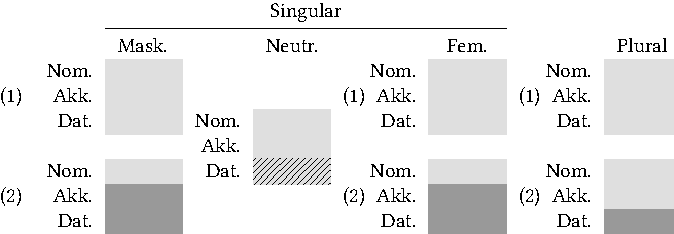
\includegraphics[width=\textwidth]{figures/fig7-6.pdf}
\caption{Paradigmenkonstellation der Substantivflexion im Singular und Plural (vgl. \citealt[88]{Rowley1997})}
\label{fig:8}
\end{figure}

Das distinkte Singular-Kasusparadigma (2) der Feminina umfasst nur eine kleine Klasse: die Verwandtschaftsbezeichnungen \textit{Mutter} und \textit{Schwester}. Nach \citet[137]{Rowley1997} flektieren auch \textit{Tochter} und \textit{Schwieger} ‚Schwiegermutter‘ sowie die mask. Verwandtschaftsbezeichnungen \textit{Bruder}, \textit{Gevatter}, \textit{Schwager}, \textit{Vater}, \textit{Vetter} nach dem Muster der schwachen Deklination, sodass im südlichen Nordbair. und im Mittelbair. eine semantisch konditionierte Deklinationsklasse ‚enge Verwandtschaftsbezeichnungen‘ anzusetzen ist (vgl. \citealt[122]{Steininger1994} und \sectref{sec:8.3.2.2}.). \mapref{map:25} zeigt, dass sich diese Paradigmenkonstellation nur im nord\-bair.-""mit\-tel\-bair. Übergangsgebiet und vereinzelt im Mittelbair. findet, die Paradigmenkonstellation (1) mit synkretischem Singularparadigma und Plural mit Nasalsuffix ist im Nordbair. und in Teilen des Ofr. belegt.{\interfootnotelinepenalty=10000\footnote{In den BSA-Erhebungen wurde für \textit{Mutter} nur die Dativ-Singular-Form abgefragt. Nach \citet[137]{Rowley1997} stellen die schwach flektierenden Feminina insofern eine Besonderheit dar, als die Akkusativ-Singular-Form (als bei den schwachen Maskulina) keine Markierung aufweist. Der vermutete Synkretismus in den eigenen Tiefenbohrungspunkten wird durch Schraffur dargestellt.}}
Daneben ist vereinzelt im Mittelbair. eine Art Mischparadigma mit Nasalflexiv im Dat.Sg. und Umlautplural belegt.\footnote{Ein solches Mischparadigma führt \citet[88]{Eich1925} auch für das Maskulinum \textit{Tropf} „‚nichtswürdiger Kerl‘“ an: schwache Deklination (d.\,h. vokalisch realisiertem Nasalsuffix) im Singular, Umlautmarkierung im Plural (Dat.Sg. \teuthoo{mI5de.An}{mideͅαn} \teuthoo{dro3bfe}{drŏbfe}, Pl. \teuthoo{dre3bf}{drĕbf}).}

\begin{map}
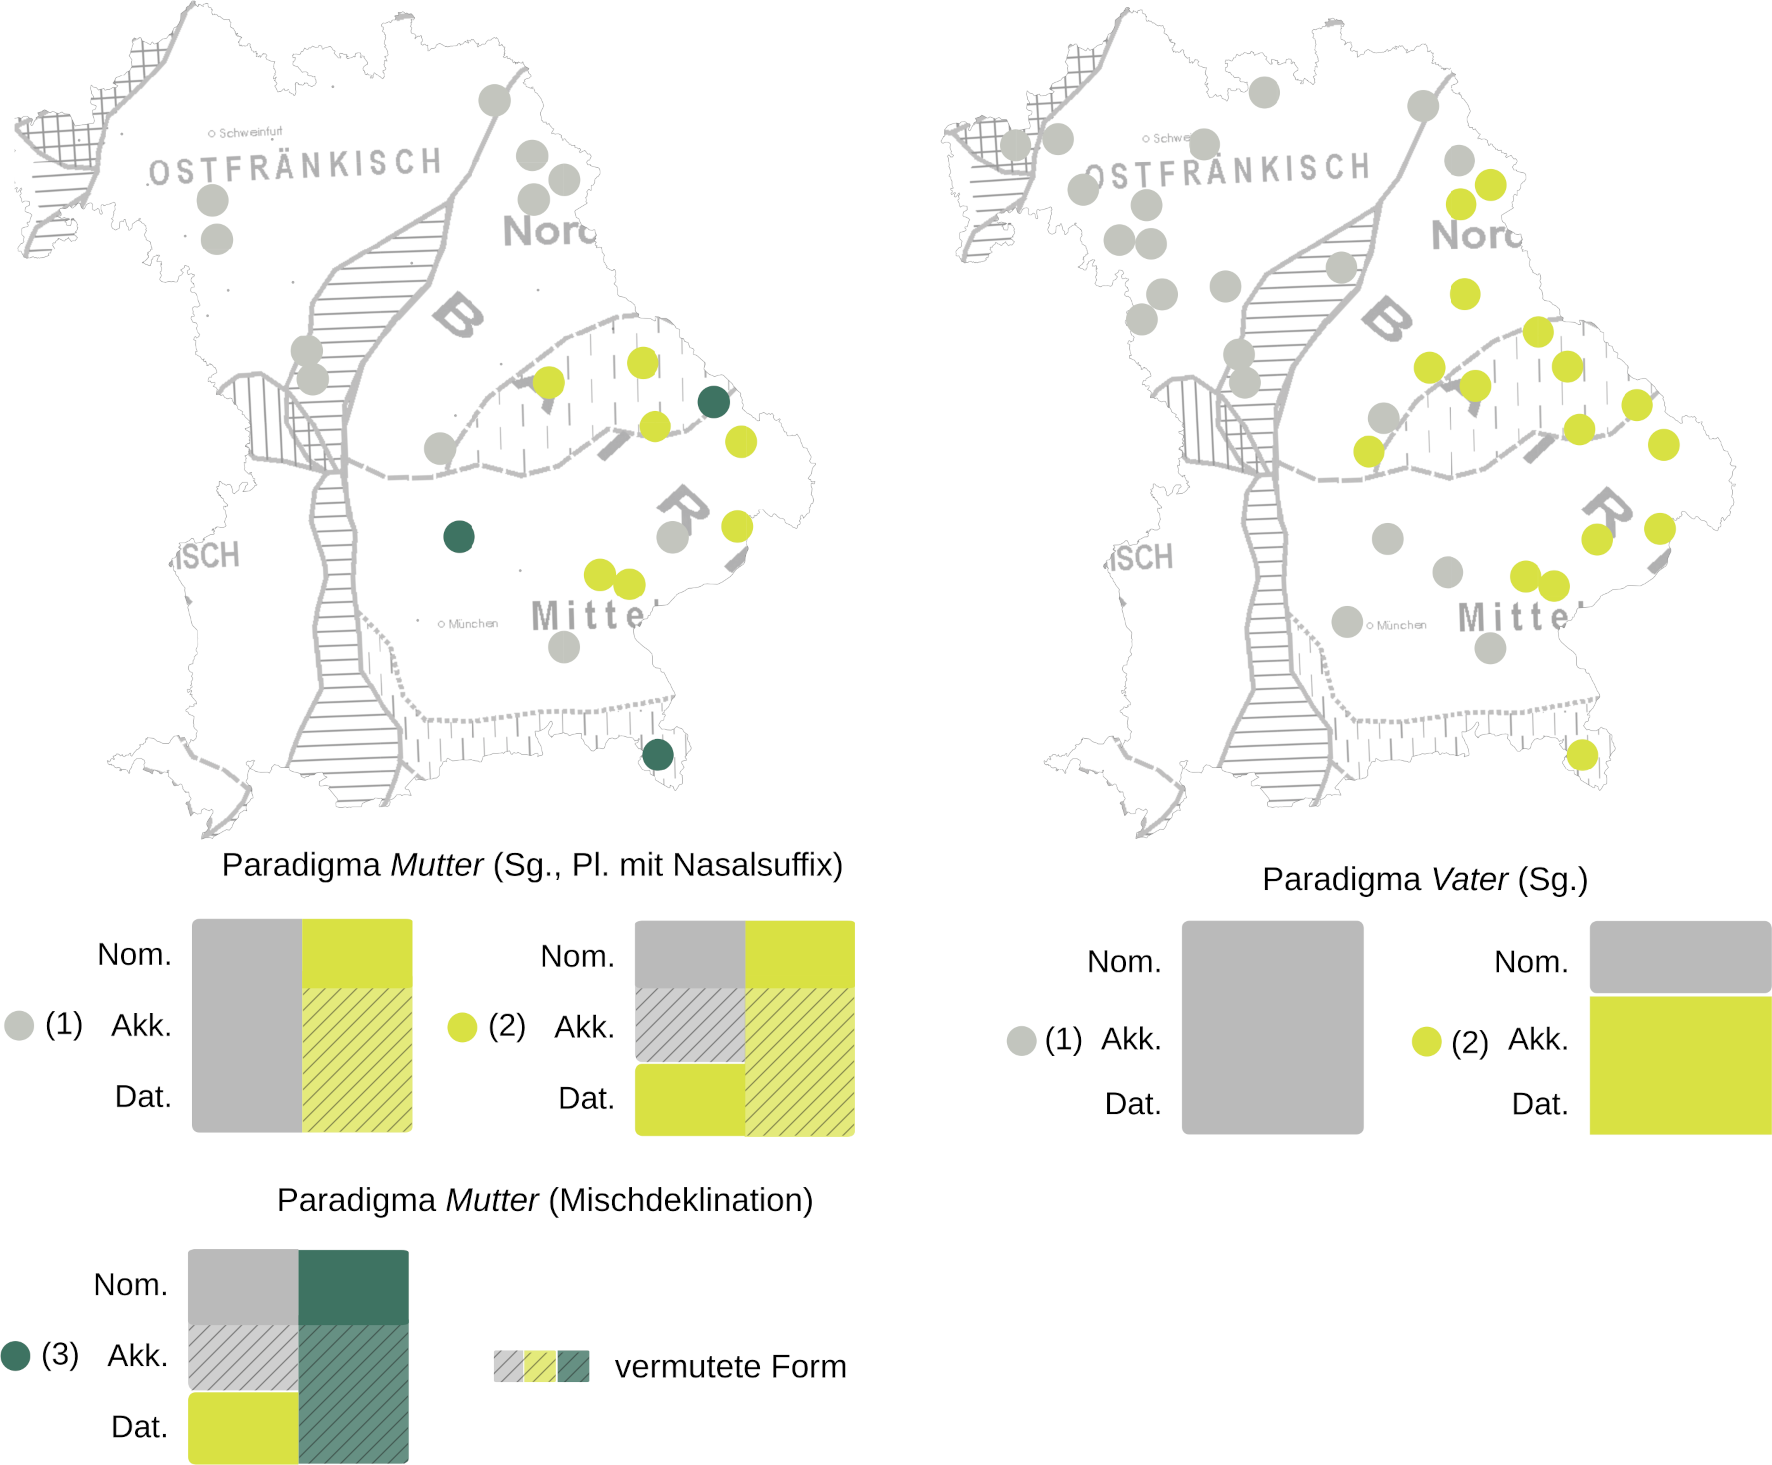
\includegraphics[width=\textwidth]{figures/Karte25.png}
\caption{Areale Verteilung der Paradigmen der schwachen Verwandtschaftsbezeichnungen \textit{Mutter} und \textit{Vater}}
\label{map:25}
\end{map}


Das Maskulinum \textit{Vater} gehört ebenfalls zu der semantisch konditionierten Deklinationsklasse „Verwandtschaftsbezeichnungen“. Die Verbreitung der distinkten Akkusativ- und Dativ-Singular-Formen ist hier noch größer als bei \textit{Mutter} (Pluralformen wurden in den BSA-Erhebungen nicht abgefragt). Bemerkenswert sind die Fälle von intraindividueller Variation, die sich (zumindest vor der Folie der schriftsprachlichen Kasusrelationen) für die in verschiedenen Kontexten abgefragten obliquen Kasusformen von \textit{Vater} und auch in der Form der Artikel in den bair. Ortsdialekten ergeben, z.\,B. exemplarisch im nordbair. Windischeschenbach \teuthoo{dEi.}{dəiͅ} \teuthoo{ho)4m}{ho\klammeruntenpost{}̣m} \teuthoo{unEm}{unəm} \teuthoo{våtEn}{v{\burgeroalpha}tən} \teuthoo{g\_ul.d5}{ɡʰulͅd̩} ‚sie haben unseren Vater vom Feld geholt‘, \teuthoo{dEi.}{dəiͅ} \teuthoo{hôo2.o4d}{h{\aufstrih}ōͅọd} \teuthoo{qi>ErEm}{ʔîərəm} \teuthoo{våtA}{v{\burgeroalpha}tα} \teuthoo{qå"glu.<EN}{ʔ{\burgeroalphamakron}ɡlûͅəŋ} ‚sie hat ihren Vater angelogen‘, \teuthoo{i“BA}{ī{\btilde}α} \teuthoo{qi>ErEn}{ʔîərən} \teuthoo{våtAn}{v{\burgeroalpha}tαn} \teuthoo{gs\#imb5f,d}{ɡšimb̩f͓d} ‚über ihren Vater geschimpft‘.

Neben den schwachen Flexionsformen dieser kleinen Klasse von Substantiven finden sich Paradigmenkonstellationen dieses Typs bei den mhd. schwachen Maskulina. Eine Schwierigkeit bei der Auswertung der schwachen Maskulina besteht in der Datenlage. Nicht alle Lexeme wurden in allen Teilprojekten in der Akkusativ-Singular-Form abgefragt, für die SNiB- und SOB-""Tie"-fen"-boh"-rungs"-punk"-te sind nur ein bis zwei Formen belegt, sodass die Datenauswertung für dieses Gebiet unbefriedigend bleibt.


\begin{map}
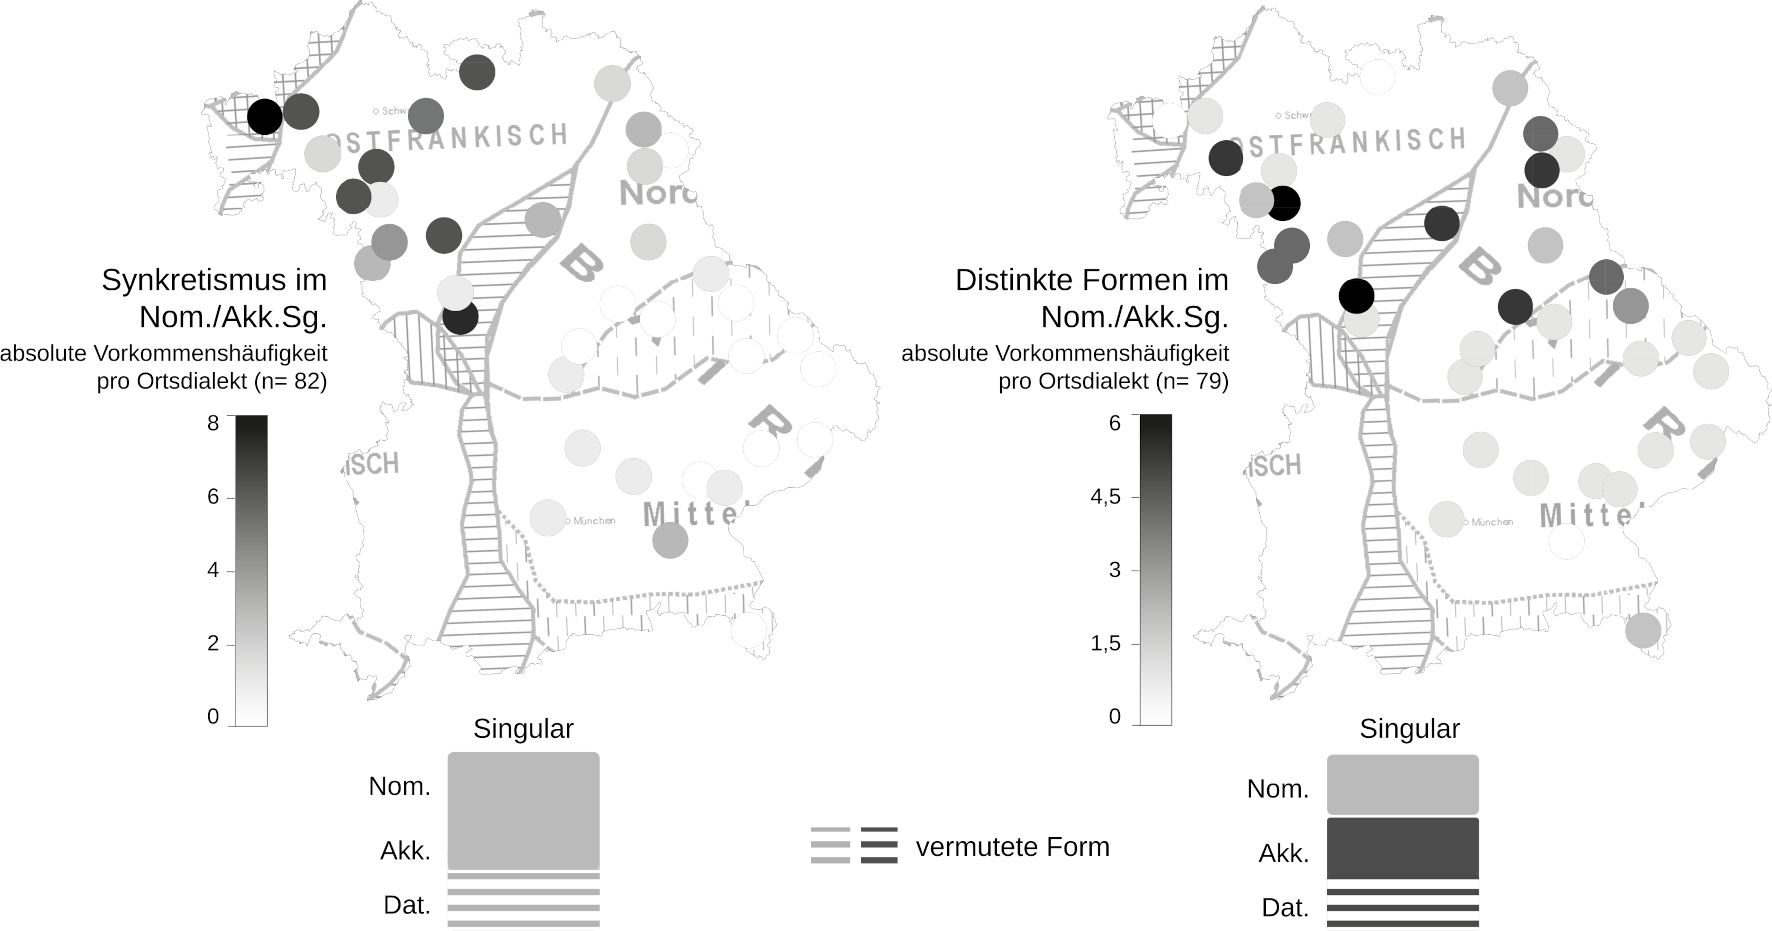
\includegraphics[width=\textwidth]{figures/Karte26.png}
\caption{Synkretismen und Distinktionen Singularparadigma der schwachen Maskulina (\teuthoo{n=}{ǹ} 161)}
\label{map:26}
\end{map}

\mapref{map:26} visualisiert in Form von Chloroplethkarten die Verteilung der beiden möglichen Paradigmenkonstellationen in absoluten Zahlen (Synkretismus durch Nullmarkierung im Akk.Sg. und Dat.Sg. vs. Distinktion durch additive Markierung).\footnote{Die Dativ-Singular-Form wurde in den BSA-Erhebungen leider nicht abgefragt, siehe aber beispielsweise \citet[§20]{Micko-Repp1933} oder \citet[§7]{Schübel1955} zu vollständigen Paradigmen.}  Im Ofr. gibt es die Tendenz zu Synkretismen. Im ofr. Ahorn und im ofr. Wiesthal gibt es keine Belege für distinkte Singularparadigmen; die Markierung der obliquen Singularkasus ist hier abgebaut. In den nordbair. Tiefenbohrungspunkten mit guter Datenlage gibt es eine eindeutige Tendenz zu distinkten Paradigmen, während es im westlichen Streifen des Ofr. ein Nebeneinander synkretischer und distinkter Formen gibt, das durch die semantische Distinktion [+belebt] und [${\pm}$menschlich] konditioniert ist (hierzu ausführlicher \sectref{sec:8.3.2.2}).

Auch \citet[183]{HarnischRowley1990} zeigen, dass die areale Verteilung distinkter obliquer Formen in der schwachen Deklination durch die semantischen Merkmale [+belebt] und [+menschlich] gesteuert ist. In einem südlichen oberofr. Gebiet (um Bamberg, Kronach) erscheint eine distinkte Markierung bei belebten Maskulina (\textit{Bube}, \textit{Hase}), im nordöstlichen oberofr. Gebiet um Coburg (Tiefenbohrungspunkt Ahorn) erscheinen synkretischen Formen. In einer Übergangszone (um Marktgraitz, Lichtenfels) zwischen diesen beiden Gebieten mit distinkter vs. synkretischer Form werden nur belebte, menschliche Denotate schwach flektiert (d.\,h. \textit{Bube}, nicht aber \textit{Hase}, vgl. \citealt[155 und 191]{Rowley1997}). Das Mosaik-Plot in  \figref{fig:9} visualisiert die Variablen Lexem, Form der Markierung im Akk.Sg. und absolute Häufigkeit. Die Größe der Flächen der Rechtecke ist dabei relativ zur Häufigkeit der Lexeme in den Daten zu lesen. Damit bestätigt das Plot -- ohne Berücksichtigung der arealen Dimension -- den Befund, dass Maskulina mit der Semantik [+belebt] und [+menschlich] eher distinkte Akkusativ-Singular-Formen aufweisen, aber auch, dass synkretische vs. distinkte Paradigmen darüber hinaus lexikalisch oder durch Frequenzeffekte bedingt zu sein scheinen (vgl. \mapref{map:30} für die areale Dimension).\footnote{Daneben werden „Abweichungen“ vom „vorherrschenden Kasussynkretismus“ im SMF auf Unsicherheiten der Gewährspersonen zurückgeführt \citealt[19]{SMF7}).}


\begin{figure}
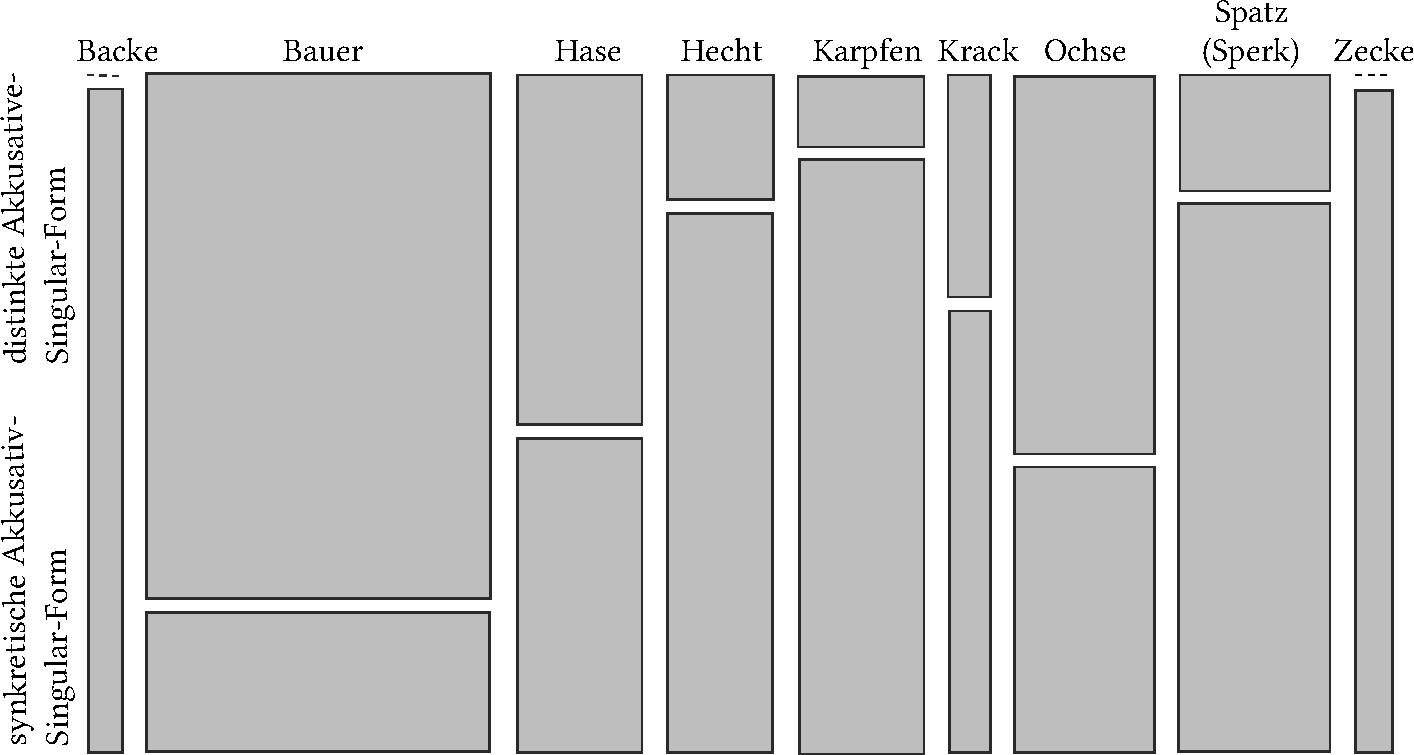
\includegraphics[width=\textwidth]{figures/revisedNickelNominalmorphologie-img038.pdf}
\caption{Mosaik-Plot mit Häufigkeitsverteilung der Akkusativ-Singular-Markierung der schwachen Maskulina ($n=164$)}
\label{fig:9}
\end{figure}

Daneben bedingt im Falle von \textit{Karpfen} die zweisilbige Struktur auf Reduktionssilbe mhd. -\textit{en} die Markierung im Ofr. und im Nordbair. und damit die Paradigmenzusammensetzung aus distinkten und synkretischen Formen (vgl. \sectref{sec:7.2.1}). Im Ofr. liegt Paradigmenkonstellation (1) mit völligem Synkretismus von Numerus und Kasus (Typ \textit{Karpfen} -- \textit{Karpfen}) vor, in Teilen des Nordbair. hingegen ergibt sich ein distinktes (dialektspezifisches) Paradigma (2) mit schwacher Markierung in den obliquen Kasus im Singular und im Plural (\figref{fig:10}). Vergleicht man diese Konstellation nun mit dem Paradigma von \textit{Eiche}, so ergeben sich ähnliche und wiederum dialektspezifische Konstellationen. \textit{Eiche} gehört im Mittelhochdeutschen zur starken Deklination, in den rezenten Dialekten des UGs flektiert es wie die nhd. Klasse der zweisilbigen Feminina mit Schwa-Reduktionssilbe (siehe \sectref{sec:7.1.3.1} zur Problematik des Bezugssystems). Im Ofr. findet sich völliger Synkretismus in Numerus und Kasus, in den bair. Ortsdialekten ist mehrheitlich Paradigma (2) mit einer distinkten Form im Plural belegt (Typ \teuthoo{oAxA}{oαxα} -- \teuthoo{oAxAn}{oαxαn}). Daneben finden sich im Bair. zwei distinkte Paradigmen: (3) im nordbair.-mittelbair. Grafenkirchen und (4) im mittelbair. Reischach. Damit sind distinkte Paradigmen bei den Feminina nicht nur bei Verwandtschaftsbezeichnungen anzunehmen, sondern auch bei nhd. zweisilbigen Feminina mit Schwa-Reduktionssilbe -- in welchem Umfang muss mit Blick auf die Datenlage leider offenbleiben.

\begin{figure}%7.8
\begin{tabular}{@{}p{0.5\textwidth}@{}p{0.5\textwidth}@{}}
  \vspace{0pt} 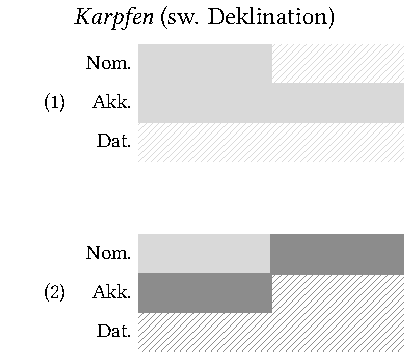
\includegraphics[width=0.49\textwidth]{figures/fig7-8-1.pdf} &
  \vspace{0pt} 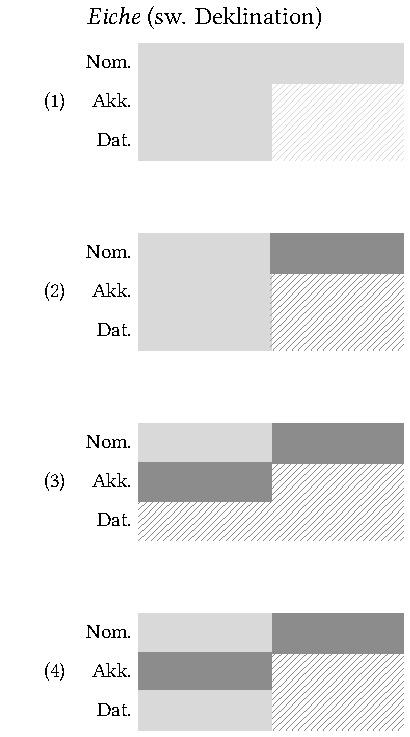
\includegraphics[width=0.49\textwidth]{figures/fig7-8-2.pdf}
\end{tabular}
\caption{Schwache Paradigmenkonstellation bei Reduktionssilbe mhd. -\textit{en}}
\label{fig:10}
\end{figure}

Laut \citet[91]{Rowley1997} werden Akkusativ und Dativ in ihren jeweiligen syntaktischen Funktionen als direktes bzw. indirektes Objekt in den Dialekten seines nordostbayrischen UGs differenziert, wenngleich sich eine Aufhebung der formalen (d.\,h. morphologischen) Distinktion beider Kasus andeute.\footnote{Auch für das unterofr. Aschenroth (Tiefenbohrungspunkt Gemünden am Main) gibt \citet[16]{Köhler1934} einen fast durchgehenden Zusammenfall von Dativ und Akkusativ an, bemerkt aber, dass der Dativ trotzdem „im Sprachgefühl noch vom Akkusativ unterschieden“ werde.}  Im Ofr. und im Regensburger Umland sei das Elizitieren additiver Dativ-Plural-Formen schwieriger als im nördlichen Nordbair. gewesen (d.\,h. in jenem Gebiet, für das \mapref{map:24} den höchsten Anteil distinkter Dativ-Plural-Formen ausweist), junge Dialektsprecher im ofr. Bayreuth und Coburg sowie im nordbair. Amberg und Regensburg hielten die additiven Formen für falsch und nicht basisdialektal \citep[95]{Rowley1997}. Für den Dat.Pl. führt \citet[441]{Schirmunski1962} im Mittelbair. eine Verdrängung durch den Akkusativ an, und auch \citet[83]{Bachmann2000} berichtet für das nordbair. Eslarn von einem intergenerationellen Wandel: Bei jüngeren Sprechern wird Dativ zunehmend durch die Akkusativform ersetzt (\textit{mitːi moe̯tlə} ‚mit den Mädchen‘), ältere und zum Teil mittelalte Sprecher verwenden die Dativform: \textit{mi moe̯tlən} (vgl. \citealt[32]{Vogt1930}).\footnote{Auch für den ofr. Dialekt Schweinfurts führt \citet[67]{Kemmeter1924} einen Zusammenfall von Dat. und Akk.Pl. zugunsten des Akkusativs an: \teuthoo{i}{i} \teuthoo{so2xs}{sōxs} \teuthoo{mainE}{mainə} \teuthoo{gro.sE}{ɡroͅsə} \teuthoo{brü"EdE}{br{\burgershwaumakron}ədə} ‚ich sag’s meinen großen Brüdern‘, \teuthoo{i}{i} \teuthoo{ho.s}{hoͅs} \teuthoo{dE}{də} \teuthoo{a.ldE}{aͅldə} \teuthoo{lo.it}{loͅit} \teuthoo{gam}{ɡam} ‚ich habe es den alten Leuten gegeben‘.} Gleichzeitig werden Formen des Akkusativs \citet[88]{Bachmann2000} zufolge noch seltener verwendet als die des Dativs, auch bei der älteren Eslarner Generation wird stattdessen die Nominativform verwendet.\footnote{Den Zusammenfall von Akkusativ und Nominativ beschreibt \citet[35]{Hirsch1958} teilweise auch für den ofr./ofr.-hess. Spessart, z.\,B. \textit{gā mor əmōl dar hōmr} ‚gib mir mal den Hammer‘.} Nur bei den schwach deklinierenden Maskulina werde Akkusativ am Substantiv markiert. Daneben interpretiert \citet[§51]{Hain1936} für das ofr. Rednitzgebiet die Markierung der Form \textit{giwin di laid} ‚gib den Leuten‘ als eine Art Übergangsform: Nachdem die Dativ-Plural-Markierung der Form \textit{gibn laidna} als „nicht mehr deutlich genug“ wahrgenommen wurde, wurde der Artikel zusätzlich zum klitisierten Artikel in \textit{giwin} noch einmal in der synkretischen Nominativ-/Akkusativform \textit{di} gesetzt, die additive Dativ-Plural-Markierung am Substantiv (\textit{laidna}) hingegen abgebaut.

Ausgehend von diesen Beobachtungen eines Wandels der Kasusmarkierung am Substantiv in den untersuchten Dialekten lautet -- mit Blick auf die Morphosyntax der Nominalphrase und den Sprachgebrauch -- eine Forschungsfrage: \textit{Inwieweit tolerieren Flexionssysteme Synkretismen?} \citet[440]{Schirmunski1962} stellt für die Dialekte des Deutschen fest, „daß eine einheitliche Tendenz zur Festigung dieser Kasusform dort wirksam ist, wo sie als indirektes Objekt ohne Präpositionen verwendet wird und ihre alten morphologischen Merkmale verloren hat.“ In den Dialekten des UGs besteht ein Nebeneinander von distinkten und synkretischen Substantivformen, die Tendenz geht in Richtung eines Abbaus der Markierung am Substantiv. Anhand des Dat.Pl. zeigt \citet[96]{Rowley1997}, dass es „im weiteren Sinne pragmatische Faktoren“ (d.\,h. den morphosyntaktischen Kontext betreffende Faktoren) sind, die die Wahl von distinkten oder synkretischen Formen bedingen können. Distinkte Dativ-Plural-Formen sind im Rahmen der Datenerhebung demnach leichter zu elizitieren und häufiger belegt (1) in Syntagmen ohne Artikel (z.\,B. nach Präposition, vgl. \teuthoo{mi}{mi} \teuthoo{k\_i“ErAn}{kʰīərαn} ‚mit Ketten‘ im nordbair. Windischeschenbach) und (2) im Vorfeld des Satzes (z.\,B. „\textit{den Kühen} habe ich’s gegeben“, „\textit{den Mädchen} werde ich’s sagen“, \citealt[96]{Rowley1997}). Im Satzvorfeld markiert die distinkte „Sonderform“ \citet[96]{Rowley1997} zufolge die syntaktische Funktion als Dativobjekt (und eben nicht als Subjekt), in artikellosen Syntagmen disambiguiert das Dativ-Plural-Suffix die Numerusinformation, vgl. die synkretischen Formen für ‚Kette‘ im nordbair. Windischeschenbach: Nom.Sg. \teuthoo{g\_i“En}{ɡʰīən} -- Dat.Sg. \teuthoo{mitE}{mitə} \teuthoo{g\_i“En@}{ɡʰīən̥} -- Nom.Pl. \teuthoo{g\_i“En@}{ɡʰīən̥} vs. die distinkte Form \teuthoo{mi}{mi} \teuthoo{k\_i“ErAn}{kʰīərαn} (siehe hierzu auch \sectref{sec:9.1}). Diese fakultative Form der Verwendung, um die Numerusinformation in Dativ-Plural-Formen auf Nasal zu disambiguieren, beschreiben auch \citet[§13]{Schübel1955} für das ofr. Stadtsteinach und \citet[§12]{Weitzenböck1942} für das mittelbair. Mühlheim: ofr. \textit{en báuen kǫsdɒ šö dráun} ‚dem Bauern kannst du schon trauen‘ vs. \textit{en báuenɒ} (oder \textit{di báuen}) \textit{kǫsdɒ šö dráun} ‚den Bauern kannst du schon trauen‘, mittelbair. \teuthoo{mim}{mim} \teuthoo{bu2Am}{būαm} in der Bedeutung ‚mit dem‘ oder ‚mit den Buben‘ neben Dat.Pl. \teuthoo{mim}{mim} \teuthoo{bu2AmA+n}{būαmα̃n}. Bemerkenswert ist an Schübels Beispiel \textit{en báuen}/\textit{en báuenɒ} und ebenso bei der distinkten Dativ-Plural-Form \teuthoo{den}{den} \teuthoo{glan}{ɡlan} \teuthoo{ma2dlana}{mādlana} ‚den kleinen Mädchen (habe ich’s gegeben)‘ (ofr. Hallerstein), wo das Dativobjekt jeweils im Satzvorfeld erscheint, dass die Kasusinformation des Dat.Pl. durch die Artikelform markiert wird. Eine fakultative Markierung disambiguiert in diesen Fällen weniger die syntaktische Funktion (Subjekt vs. Objekt), sondern die Numerusinformation (vgl. Schübels Variante Nom./Akk.Pl. \textit{di báuen kǫsdɒ šö dráun}). Eine fakultative distinkte Dativ-Plural-Form entspräche demnach weniger \citegen[97]{Rowley1997} Formel „Dat.Pl. nur dort flektiert, wo keine andere Kasusexponenz vorliegt“, sondern der fakultativen Pluralmarkierung, wie sie in den bair. Dialekten beispielsweise bei den mhd. schwachen Feminina zu finden ist (ausführlicher hierzu \sectref{sec:9.2}).

\chapter{Dialektale Deklinationssysteme in den ostoberdeutschen Dialekten Bayerns}
\label{chap:8}
Deklinationsklassen stellen eine abstrakte Klassifikation von Substantiven dar, welche sich dieselben formalen Flexionsmarker im Paradigma teilen (vgl. \chapref{chap:3}.). Für die Einteilung der mhd. oder nhd. Deklinationsklassen werden „mehr oder weniger zwangsläufig“ (\citealt[71]{KleinEtAl2018}) die Kasusexponenten des Genitiv Singular und die Pluralallomorphe herangezogen, da im Singularparadigma der Genitiv am stärksten distinkte Formen und ein vergleichsweise ausdifferenziertes Markerinventar aufweist; im Pluralparadigma ist bereits im Mittelhochdeutschen nur noch das uniforme Nasalsuffix im Dativ erhalten. Infolge des weitgehenden Abbaus der Kasusmarkierung am Substantiv und verschiedener innerparadigmatischer Ausgleichsprozesse (z.\,B. Übernahme des Flexivs der obliquen Kasus in den Nom.Sg.) berücksichtigen synchrone Klassifikationen dialektaler Flexionssysteme in der Regel nur die Pluralallomorphie, da diese als „einzig klares Kriterium“ verbleibe, wie es beispielsweise \citet[41]{White1966} in seiner Grammatik zum mittelbair. Dialekt von Eisenhofen formuliert. In den rezenten Dialekten handelt es sich also vielmehr um „Pluralbildungsklassen“ \citep[170]{Rowley1997} als um Deklinationsklassen, wie sie historisch in den Sprachstufen des Deutschen zu finden waren. Gleichzeitig manifestieren sich Deklinationsklassen auch in den rezenten Dialekten des Untersuchungsgebiets in zwei Ausprägungen:

\begin{itemize}
\item Die historische Klassenzugehörigkeit ist bewahrt, aufgrund dialektspezifischer phonologischer Prozesse hat in den untersuchten Dialekten aber eine Erhöhung des Inventars morphophonologischer Pluralmarker stattgefunden, sodass die rezenten Entsprechungen der Numerusexponenten der historischen Klassen in der arealen Dimension formal variieren.
\item Diachron hat sich Deklinationsklassenwandel vollzogen, und zwar in Form von Deklinationsklassenwechsel oder weil sich -- teilweise dialektraumspezifische -- außerflexivische Konditionierungsfaktoren herausgebildet haben, die wiederum zu Deklinationsklassenwechsel führten.
\end{itemize}

In der folgenden Darstellung werden die synchrone und diachrone Perspektive, die sich an diesen beiden zentralen Befunden ablesen lässt, konsequent beibehalten. Die dialektalen Deklinationsklassen werden im Folgenden zunächst in ihrer synchronen Zusammensetzung (\sectref{sec:8.1}) und anschließend in ihrer diachronen Entwicklung (\sectref{sec:8.2}) behandelt. \sectref{sec:8.3} fokussiert schließlich die Zusammensetzung der Deklinationsklassen und die Rolle außerflexivischer Faktoren, stets unter Berücksichtigung der arealen Dimension.

\section{Synchrones dialektales Deklinationsklassensystem}
\label{sec:8.1}
Die Darstellung der Formenbildung in \chapref{chap:7} hat gezeigt, dass sich das Pluralmarkerinventar in den untersuchten Dialekten infolge verschiedener historischer phonologischer Prozesse (insbesondere im Bereich der stammaffizierenden Verfahren) ausdifferenziert hat, dass damit synchron Heteromorphie zu beobachten ist. Gleichzeitig wird die Markierung der Kasusinformation am Substantiv in der Tendenz abgebaut, wenngleich auch hier -- nämlich im Falle des Dat.Pl. -- eine dialektspezifische Ausdifferenzierung des additiven Markerinventars stattgefunden hat. Der Abbau der Kasusmarkierung am Substantiv hat in den untersuchten Dialekten noch nicht zu einem vollständigen Verlust der Kasusmarkierung am Substantiv geführt, doch vor allem im Singularparadigma findet sich weitgehender Formensynkretismus; eine distinkte Kasusform ist nur bei den Maskulina im Akkusativ/Dativ zumindest teilweise erhalten, bei den Feminina findet sie sich zum Teil im Dat.Sg. (vgl. \sectref{sec:7.2.2}). Ein synchrones Deklinationssystem der oobd. Dialekte basiert aufgrund dieser sprachinternen Entwicklungen vor allem auf der Pluralallomorphie. Hinzu kommt, dass für die untersuchten Dialekte keine konsistenten Daten zur Kasusflexion im Singular vorliegen, sodass auch aus methodischen Gründen primär die Pluralmarkierung herangezogen werden muss. Da, wo es möglich ist (d.\,h. bei Maskulina der historisch schwachen Deklination, wo Singular-Kasusformen systematisch abgefragt wurden), werden auch Aussagen zur Kasusexponenz des Singulars oder zu spezifischen Paradigmenkonstellationen getroffen. Ausgehend von diesen Überlegungen und auch mit Blick auf die Definition des Klassifizierungsprinzips Deklinationsklasse (\chapref{chap:3}) ist die zentrale Frage der Klasseneinteilung: Wie ähnlich muss das Flexionsverhalten sein, damit Substantive eine Klasse bilden?

Die Bezeichnung der rezenten dialektalen Deklinationsklassen orientiert sich an den formalen Ausprägungen der Klassen (im diachronen Bezug werden allerdings germ. Klassenbezeichnungen verwendet, vgl. \sectref{sec:8.2}). Ich folge darin \citet[27]{Rowley1997} und \citet[124]{Wurzel1984}, die sich jeweils dafür aussprechen, Deklinationsklassen nach den spezifischen Klassenmerkmalen oder -eigenschaften zu benennen. Die Idee des vorgeschlagenen synchronen Deklinationsklassensystems ist es, die Analyse auf mehreren Ebenen zu ermöglichen. Die oberste Ebene bilden Klassentypen, deren Bezeichnung sich an den Pluralmarkierungsverfahren orientiert (\figref{fig:11}): NULL, die additiven (nach den Allomorphen bezeichneten) Klassen N, A, E, R und die stammaffizierende Klasse MOD („modulativ“).\largerpage

Auf dieser Ebene wurde die Differenzierung der additiven Pluralmarker Nasalsuffix, Schwa und Tiefschwa sowie \textit{er}{}-Suffix beibehalten. Diese Lösung wurde gewählt, um die Distribution und Zusammensetzung der verschiedenen additiven Deklinationsklassen dialektübergreifend analysieren zu können. Der methodische Nachteil dieser Form der Klassifikation ist, dass die Heteromorphe \mbox{-\textit{n}}, -\textit{ə} und -\textit{α} als rezente Entsprechungen des Nasalsuffixes (etwa bei \teuthoo{hosn}{hosn}, \teuthoo{hosE}{hosə} oder \teuthoo{hosA}{hosα} ‚Hasen‘) der his\-to\-risch schwachen Maskulina oder die Heteromorphe -\textit{(ə)r}, -\textit{ə} und -\textit{α} als rezente Entsprechung des \textit{er}{}-Suffixes der his\-to\-rischen \textit{iz/az}{}-Klasse (\teuthoo{haisEr}{haisər}, \teuthoo{haisE}{haisə}, \teuthoo{haisA}{haisα} ‚Häuser‘) jeweils unterschiedlichen Klassen zugeordnet werden (siehe \sectref{sec:7.1.1.1} zum Suffixinventar, vgl. \citealt[129]{Rowley1997}). Wo es sinnvoll ist, die Heteromorph-Ebene zu abstrahieren, d.\,h. v.\,a. in der Darstellung des Deklinationsklassenwandels (\sectref{sec:8.2}), wird diese differenzierte Klasseneinteilung zu dialektübergreifenden Klassen zusammengefasst.


\begin{figure}
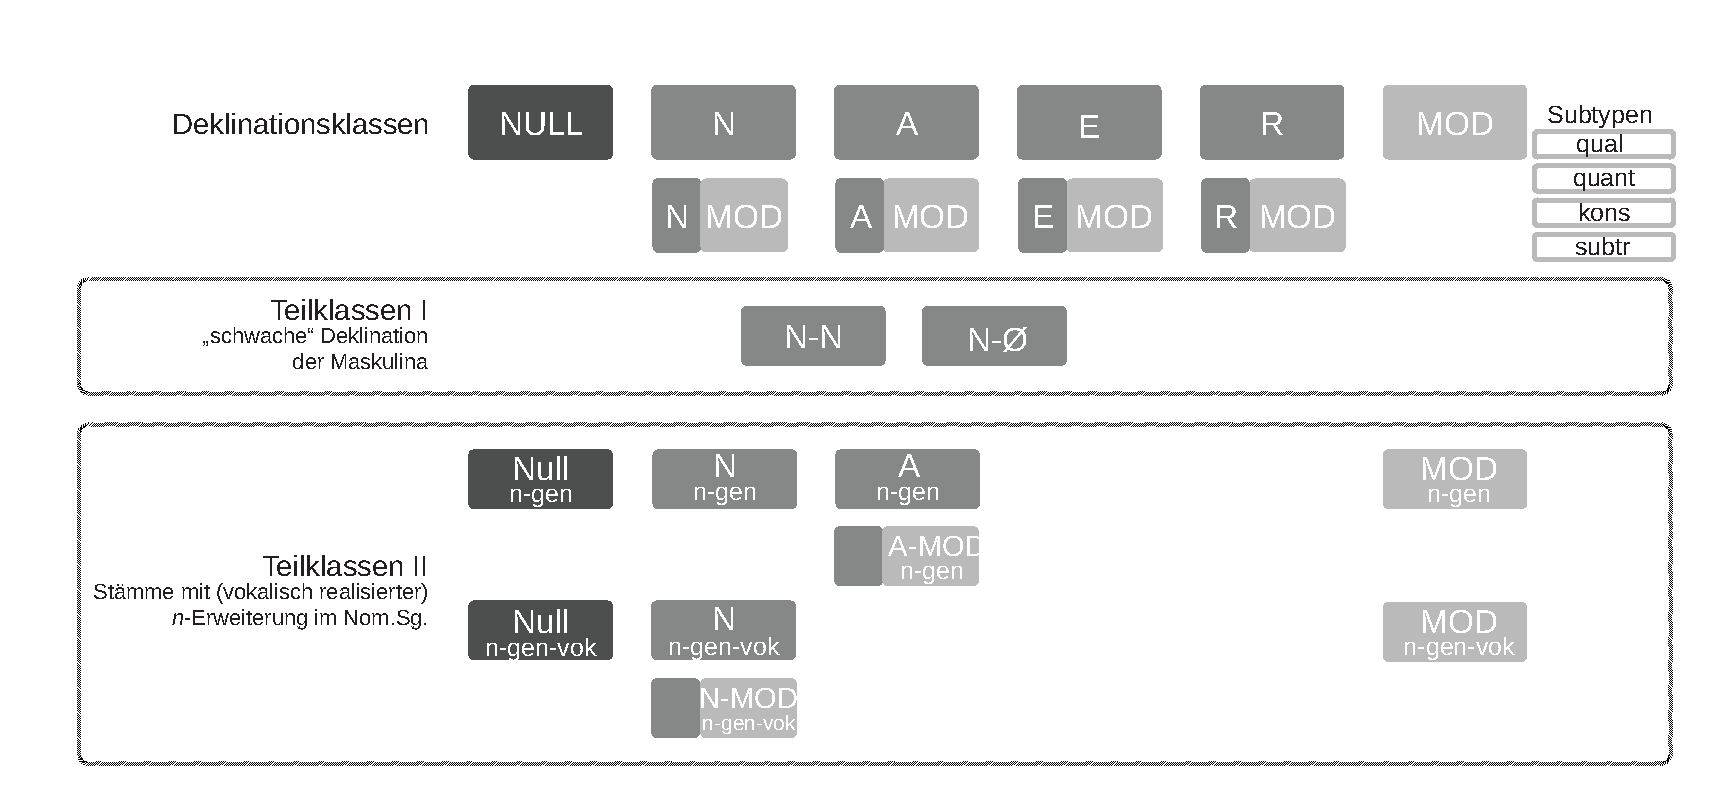
\includegraphics[width=\textwidth]{figures/Deklinationsklassen.pdf}
\caption{Synchrone dialektale Deklinationsklassen}
\label{fig:11}
\end{figure}

Auch in der stammaffizierenden Klasse MOD wird Heteromorphie, d.\,h. dialektspezifische morphophonologische Alternationen, in Form von vier Untertypen berücksichtigt. Die Klasse MOD(qual) umfasst sämtliche Alternationen der Vokalqualität, d.\,h. Umlaut, Wechsel der Zungenhöhe sowie die umlautähnliche Alternation von mhd. \textit{ei}, MOD(quant) bezeichnet Alternationen der Vokalquantität, MOD(kons) sämtliche Alternationen des Konsonantismus (Le"-nis-""For"-tis-""Kon"-tras"-te, 0/K- und K/0-""Al"-ter"-na"-tio"-nen, Spirantisierungen) und MOD"-(subtr) subtraktive Formen. Treten mehrere stammaffizierende Verfahren kombiniert auf, sind diese Subtypen entsprechend annotiert, sodass die Analyse je nach Fragestellung sowohl die übergeordnete Ebene des Klassentyps MOD als auch die konkret realisierten Verfahren der Subtypen berücksichtigen kann, z.\,B. MOD"-(kons, qual, quant) bei \teuthoo{bo.2}{bōͅ} -- \teuthoo{ba4X!}{bạꭖ} ‚Bach‘ (nordbair.-mittelbair. Bernhardswald).

Für die Datenauswertung ist die Idee hinter dieser mehrstufigen Klassenbezeichnung, eine Analyse von einer abstrahierenden Ebene hin zu feineren Abstufungen zu ermöglichen, die einerseits die Kombination von Markierungsverfahren erfasst und zum anderen areal variierende Ausprägungen der einzelnen stammaffizierenden Strategien im Blick hat. Gleichzeitig versucht diese Klassifizierung der mentalen Repräsentation von Flexionsformen nahezukommen. Aus Perspektive einer Dialektgeografie ist es relevant und interessant, welche phonologischen Prozesse historisch zu den morphophonologischen Alternationen bei \teuthoo{kha."+mb\_}{khã̄ͅmbʰ} -- \teuthoo{khe.m}{kheͅm} ‚Kamm‘ (ofr.-hess. Wiesthal), \teuthoo{kha.m}{khaͅm} -- \teuthoo{kha4mb5\_}{khạmb̩ʰ} (nordbair.-mittelbair. Blaibach) oder \teuthoo{k\_a.mbv}{kʰaͅmbv} -- \teuthoo{k\_a4mpf}{kʰạmpf} (mittelbair. Kirchensur) geführt haben. In \sectref{sec:7.1.2} wurde indes gezeigt, dass innerparadigmatische Alternationen, insbesondere jene, die den stammauslautenden Konsonantismus affizieren, his"-to"-ri"-sche phonologische Prozesse konservieren und lexikalisiert sind -- mit der Ausnahme einiger weniger funktionalisierter, produktiver Verfahren wie dem Umlaut. Zudem scheint es aus Sprecherperspektive plausibel, eine einzige Klasse MOD für sämtliche stammaffizierenden Verfahren anzunehmen, und zwar in Abgrenzung von additiven Markierungsverfahren und Null.

Unterhalb der additiven und stammaffizierenden Oberklassen und der kombinierten Klassen (R-MOD, A-MOD, N-MOD, E-MOD) werden zwei Teilklassen beschrieben:

\begin{itemize}
\item In der Denomination der Deklinationsklassen werden Singularstämme, bei denen das Nasalsuffix der obliquen Kasus analog in den Nom.Sg. übertragen wurde, gesondert ausgewiesen, um spezifische Analysen zur Distribution der Pluralallomorphie für diese \textit{n}{}-erweiterten Stämme und ihren relativen Anteil in der Zusammensetzung einzelner Deklinationsklassen zu ermöglichen. Die Denomination der Klassen besteht aus einem Präfix, das das Flexionsverfahren bezeichnet (NULL, N, MOD usw.) und einem Suffix, dass die Realisierung des (historischen) Nasalsuffixes der Singularform angibt: Suffix „n-gen“ für die Realisierung als Nasal, „n-gen-vok“ für die vokalische Realisierung. Als Teilklasse der NULL-Deklinationsklasse erscheint etwa die Klasse NULL-n-gen (Typ \teuthoo{glokN}{ɡlokŋ} -- \teuthoo{glokN}{ɡlokŋ} ‚Glocke‘), als Teilklasse der N-Klasse die Klasse N-n-gen-vok (Typ \teuthoo{biEkA}{biəkα} -- \teuthoo{biEkAn}{biəkαn} ‚Birke‘).
\item Bei historisch schwachen Maskulina, für die systematisch auch oblique Singular-Kasusformen erhoben wurden, wird danach differenziert, ob Kasus eine distinkte Markierung aufweist (Teilklassen N-N) oder synkretische Formen vorliegen (N-∅). Die Denomination der Teilklasse fasst vokalische Realisierungen als Schwa oder Tiefschwa und Realisierungen als Nasalsuffix zusammen.
\end{itemize}

Eine andere grundsätzliche Frage, die sich vor allem für kombinierte Markierungsverfahren stellt, lautet: Welches Flexionsmuster ist klassenkonstituierend, welche Markierungsverfahren werden als konkomitant und damit als nicht klassenkonstituierend analysiert? Im Neuhochdeutschen etwa ist der Umlaut in Kombination mit \textit{er}{}-Suffix (Typ \textit{Huhn} -- \textit{Hühner}) konkomitant, da Umlaut obligatorisch und voll vorhersagbar bei Klassenmitgliedern mit velarem Stammvokal erscheint (vgl. \citealt[69]{Dammel2018} sowie \sectref{sec:4.1}). Hier ist es sinnvoll, eine einzige Deklinationsklasse anzusetzen, die Pluralformen mit \textit{er}{}-Suffix und UL+\textit{er} umfasst.

Für sein nordostbayerisches UG klassifiziert \citet{Rowley1997} kombinierte Markierungen in Form eines additiven und eines stammaffizierenden Markers als Teilklassen einer additiven Deklinationsklasse. So gehörten das Neutrum ofr. \teuthoo{I2sd}{ı̄sd} -- \teuthoo{I2sda}{ı̄sda} ‚Nest‘ und eine Pluralform mit Quantitätskontrast wie ofr. \teuthoo{ne2isd}{nēisd} -- \teuthoo{ne.sde.}{neͅsdeͅ} ‚Nest‘ gleichermaßen zur R-Klasse, das Flexionsmuster mit Quantitätskontrast bildet dabei eine Teilklasse R „mit Dehnung des Singularstamms“ \citep[164]{Rowley1997}. Das stammaffizierende Verfahren ist als „zusätzliche Modifikation“ konkomitant, klassenkonstituierend ist die „besondere Formenkonstellation im Paradigma“: die additive Markierung mit \textit{er}{}-Suffix \citep[145]{Rowley1997}.\footnote{Ähnlich verfährt \citet[41]{White1966}, der zwar Klassen mit vs. ohne Umlautmarkierung differenziert, aber Lenis-Fortis-Kontraste im Stammauslaut als konkomitantes Merkmal ausweist, das phonologisch bedingt ist.} Nur wenn sie ausschließlich vorkommen, konstituieren stammaffizierende Markierungen eine eigene Deklinationsklasse \citep[144]{Rowley1997}. Für eine morphologische Sprachgeografie eignet sich diese Form der Klassifikation \citet[145]{Rowley1997} zufolge, weil im Bereich der stammaffizierenden Verfahren „areal unterschiedliche Kombinationen und regional große Schwankungen beim einzelnen Lexem vorliegen können.“ Nicht unproblematisch ist aber in meinen Augen, dass der additiven Markierung der Status der „besonderen Formenkonstellation“ a priori zugesprochen wird und stammaffizierende Markierungen automatisch konkomitant sind. Hier scheint eine Differenzierung sinnvoll, wie sie \citet[65--66]{Dammel2018} für das Konkomitanzverhältnis von Umlaut und additivem Flexiv im Neuhochdeutschen beschreibt:

\begin{enumerate}[label=(\alph*)]
\item Umlaut wird entweder obligatorisch durch das Flexiv gefordert (z.\,B. beim nhd. \textit{er}{}-Plural, Typ \textit{Huhn} -- \textit{Hühner}) oder er ist durch das Flexiv ausgeschlossen (z.\,B. beim nhd. \textit{(e)n}{}-Plural). Beim \textit{e}{}-Suffix erscheint Umlaut nur bei den Feminina der historischen \textit{i}{}-Deklination (Typ \textit{Kraft} -- \textit{Kräfte}) automatisch, Neutra mit \textit{e}{}-Plural weisen (mit Ausnahme von \textit{Floß} -- \textit{Flöße}) nie Umlaut auf.
\item Umlaut „indiziert“ bestimmte Flexive (im Neuhochdeutschen -\textit{er}, -\textit{e}, -∅).
\item Umlaut und Flexiv kookkurrieren, indizieren einander und markieren die Numerusinformation gleichzeitig.
\item Umlaut und Flexiv treten unabhängig voneinander auf, z.\,B. beim mask. \textit{e}{}-Plural (\textit{Gast} -- \textit{Gäste} neben \textit{Tag} -- \textit{Tage}) und bei zweisilbigen Maskulina mit Nullplural (-∅) vs. Umlaut (UL-∅, z.\,B. \textit{Knoten} -- \textit{Knoten}, \textit{Garten} -- \textit{Gärten}).
\end{enumerate}

\begin{sloppypar}
Dass die Konkomitanzverhältnisse in den oobd. Dialekten anders spezifiziert sind als im Neuhochdeutschen, zeigen exemplarisch zwei kumulative Pluralformen aus Bernhardswald im nordbair.-mittelbair. Übergangsgebiet. Bei \teuthoo{o4<b5v5l°@}{ộb̩v̩l̥̑} -- \teuthoo{epfl°@n@}{epf‌l̥̑n̥} ‚Apfel‘ ist der additive Marker -\textit{n} mit Blick auf die his"-to"-ri"-sche Deklination sekundär (mask. \textit{i}{}-Deklination), bei \teuthoo{s\#du.2m}{šdūͅm} -- \teuthoo{ds\#di“mA}{dšdīmα} ‚Stube‘ mit \textit{n}{}-erweitertem Singularstamm sind sowohl Umlaut als auch das „potenzierte“ additive Tiefschwa-Suffix sekundär. Die oobd. Innovation besteht darin, dass Nasalsuffix und Umlaut -- anders als im Neuhochdeutschen -- kookkurrieren können (d.\,h. Dammels Typ (c)).\footnote{Im Falle der Pluralform \textit{Äpfeln} ist die „Innovation“ der Markierungsstrategie allerdings nicht jung: \citet[§36, Anmerkung 2]{Paul1968} erwähnt die schwache Singularform \textit{Äpfeln} („Birn und Äpfeln“) im 14. und 15. Jahrhundert.} Hier ist das stammaffizierende Verfahren nicht konkomitant, es wird daher eine kombinierte Deklinationsklasse N-MOD bzw. A-MOD angenommen. Ein Fall von Konkomitanz liegt dagegen bei den innerparadigmatischen Spirantisierungen (Typ \teuthoo{gro2b}{ɡrōb} -- \teuthoo{gra42wA}{ɡrạ̄wα} ‚Grab‘) oder von Obstruentenelisionen in additiven Pluralformen (Typ \teuthoo{vi“}{vī} -- \teuthoo{vi“cA}{vīXα} ‚Vieh‘) vor, da die Alternation im Falle der Spirantisierung durch synchrone phonologische Regeln ab- und der Erhalt des stammauslautenden Plosivs durch dessen phonotaktische Position hergeleitet werden können.
\end{sloppypar}

\section{Deklinationsklassenwechsel und -wandel in den oobd. Dialekten}
\label{sec:8.2}
Im Fokus des folgenden Kapitels stehen die Reorganisation des Deklinationsklassensystems und die rezenten Entsprechungen der historischen Deklinationsklassen in den untersuchten Dialekten. Konkret geht es um folgende Forschungsfragen:

\begin{itemize}
\item Welche Marker und Markierungsverfahren sind die lautgesetzlichen Entsprechungen der historischen Deklinationsklassen (und ihrer Pluralallophone) in den rezenten Dialekten? Inwiefern ist die formale Entsprechung der historischen Klassen in den rezenten Dialekten durch phonologische Prozesse bedingt, gibt es areale Unterschiede?
\item Inwiefern haben (morpho)phonologische Prozesse möglicherweise zu einer Ausdifferenzierung oder zu einem Zusammenfall der historischen Klassen geführt? Und inwiefern verhalten sich zwei Mitglieder derselben historischen Deklinationsklasse synchron gleich?
\item Gibt es diachron einen Ab- oder Ausbau des Deklinationsklassensystems? Wo sind Deklinationsklassenwechsel zu verzeichnen?
\end{itemize}

Ziel des Kapitels ist zunächst eine Inventarisierung der dialektalen Deklinationsklassen und von Deklinationsklassenwechsel. Inwiefern Deklinationsklassen diachron und synchron zu außerflexivischer Konditionierung tendieren, ist Thema des \sectref{sec:8.3}.

\begin{sloppypar}
Das Tertium Comparationis ist das mhd. Deklinationsklassensystem.\footnote{Die Zuordnung der mhd. Deklinationsklassen für die untersuchten Lemmata basiert auf den Darstellungen von \citet{Paul1968} und \citet{Lexer1872-1878}, ahd. Deklinationsklassen basieren auf den Angaben bei \citet{BrauneHeidermanns2018}.} Zwar ist im Mittelhochdeutschen hinsichtlich Deklinationsklassenzusammensetzung und Klassenwechsel ein hohes Maß an Dynamik zu beobachten (siehe \sectref{sec:3.1.2}), doch ist der mhd. Lautstand und auch das mhd. Allomorphinventar der Ausgangspunkt für dialektspezifische morphophonologische Entwicklungen, wie die Darstellung zur Formenbildung in \chapref{chap:7} gezeigt hat. Als Klassenbezeichnungen werden -- trotz des „arbiträren Etikettencharakter[s]“ \citep[73]{Kürschner2008a} -- die germ. stammbildenden Suffixe verwendet, um die Vergleichbarkeit mit anderen dialektgrammatischen Darstellungen herzustellen, wo die germ. Klassen das übliche Referenzsystem sind.
\end{sloppypar}

\subsection{Maskulina}
\label{sec:8.2.1}
Das Schwa-Suffix der mask. \textit{a}- und \textit{i}-Deklination schwindet im UG lautgesetzlich durch die einsetzende Apokope des Mittelhochdeutschen. Die Maskulina der \textit{i}{}-Deklination, die den Plural im Mittelhochdeutschen mit UL+\textit{e} markieren, weisen in den rezenten Dialekten rein stammaffizierende Pluralformen auf (siehe  \figref{fig:12} und das exemplarische Beispiel \textit{Bach}). Maskulina der \textit{i}{}-Deklination mit palatalem Stammvokal weisen trotz Umlautlosigkeit auch nach Apokopierung des Schwa-Suffixes nur teilweise Nullplural auf.\footnote{Erhalten ist der lautgesetzliche Nullplural etwa bei \textit{Docht}, \textit{Flügel}, \textit{Hobel}, \textit{Laib}, \textit{Schlüssel}, \textit{Stiefel} und im Ofr. \textit{Reif}, \textit{Stein}. Daneben kann Nullplural das Ergebnis von innerparadigmatischem Ausgleich sein.}  Vor der Apokope sind in den untersuchten Dialekten verschiedene phonologische Prozesse wirksam, die, bedingt durch die Ein- vs. Zweisilbigkeit von Singular- und Pluralformen, zu innerparadigmatischen Alternationen von Stammvokalquantität (infolge der Einsilberdehnung, im Bair. kombiniert mit Lenis-Fortis-Kontrasten) oder der Stammvokalqualität führen. So gehören etwa im ofr.-hess. Wiesthal \textit{Tisch} und \textit{Bach} zur selben Deklinationsklasse, da mhd. \textit{i} im historischen Zweisilber gesenkt ist und infolgedessen eine Alternation der Zungenhöhe und damit der Vokalqualität erscheint (\teuthoo{di“s\#}{dīš} -- \teuthoo{des\#}{deš}, vgl. \sectref{sec:7.1.2.1.3}).

\vfill
\begin{figure}[H]
\fittable{%
\begin{tikzpicture}[every node/.style={rectangle,text width=3.2cm,minimum height=1.2cm,align=center,rounded corners}]
  \node(modqual)[rectangle,draw] {\textbf{MOD}(qual)};
  \node(dk)[rectangle,draw,above=1mm of modqual,thick]{Dialektale DK};
  \node(modquant)[rectangle,draw,below=1mm of modqual]{\textbf{MOD}(quant)};
  \node(NULL)[rectangle,draw,below=1mm of modquant]{\textbf{NULL}};
  \node(A)[rectangle,draw,below=1mm of NULL]{\textbf{A}};
  \node(N)[rectangle,draw,below=1mm of A]{\textbf{N}};
%
  \node(boox)[rectangle,draw,left=1mm of modqual]{b\=ox--bax\\ofr.-hess. d\=is--deš};
  \node(diis)[rectangle,draw,below=1mm of boox]{d\=iš--diš, diʃ};
  \node(dis)[rectangle,draw,below=1mm of diis]{diš--diš};
%
  \node(bach)[rectangle,draw,left=8mm of boox]{mhd. \textit{bach}--\textit{bech\textbf{e}}\\(ahd. \textit{bah}--\textit{beh\textbf{i}})};
  \node(mask.i)[rectangle,draw,above=1mm of bach,thick]{\textbf{mask. \textit{i}}};
  \node(tisch)[rectangle,draw,below=1mm of bach]{mhd. \textit{tisch}--\textit{tisch\textbf{e}}\\(ahd. \textit{tisk}--\textit{tisg\textbf{i}})};
%
  \node(modqualhund)[rectangle,draw,right=1mm of modqual]{ofr. hund--hind\\nordbair. šdoα--šdoi};
  \node(huund)[rectangle,draw,below=1mm of modqualhund]{h\=und--hund, hunt};
  \node(nullhund)[rectangle,draw,below=1mm of huund]{hund--hund\\ofr. šd\=a--šd\v{\={a}}};
  \node(sdoa)[rectangle,draw,below=1mm of nullhund]{mittelbair. šdoα--šdoαnα};
  \node(nhund)[rectangle,draw,below=1mm of sdoa]{ofr. hund--hundn};
%
  \node(stein)[rectangle,draw,right=8mm of modqualhund]{mhd. \textit{stein}--\textit{stein\textbf{e}}\\(ahd. \textit{stein}--\textit{stein\textbf{a}})};
  \node(mask.a)[rectangle,draw,above=1mm of stein,thick]{\textbf{mask. \textit{a}}};
  \node(hunt)[rectangle,draw,below=1mm of stein]{mhd. \textit{hunt}--\textit{hund\textbf{e}}\\(ahd. \textit{hunt}--\textit{hund\textbf{a}})};
%
  \node(legende1)[below=1mm of N,text width=5cm,minimum height=1cm]{lautgesetzlicher~Wandel};
  \node(legende2)[below=1mm of legende1,text width=5cm,minimum height=1cm]{Deklinationsklassenwechsel};
%
\draw[thick](bach.east)--(boox.west);
\draw[thick](tisch.east)--(boox.west);
\draw[thick](tisch.east)--(diis.west);
\draw[thick](tisch.east)--(dis.west);
%
\draw[thick](modqualhund.east)--(stein.west);
\draw[thick](nullhund.east)--(stein.west);
\draw[thick](huund.east)--(hunt.west);
\draw[thick](nullhund.east)--(hunt.west);
\draw[dashed,thick](modqualhund.east)--(hunt.west);
\draw[dashed,thick](sdoa.east)--(stein.west);
\draw[dashed,thick](nhund.east)--(hunt.west);


\draw(legende1.west)++(-15mm,0)--(legende1.west);
\draw[dashed,thick](legende2.west)++(-15mm,0)--(legende2.west);
\end{tikzpicture}}
\caption{Lautgesetzliche Entsprechungen und Deklinationsklassenwechsel bei mask. \textit{a-} und \textit{i}{}-Stämmen (Dialektbeispiele ohne gesonderte Zuordnung des Dialektraumes erscheinen im gesamten UG)}
\label{fig:12}
\end{figure}
\vfill\pagebreak

Auch bei den mask. \textit{a}{}-Stämmen erscheinen lautgesetzlich Alternationen der Vokalqualität: Im Nordbair. weisen mask. \textit{a}{}-Stämme mit Stammvokal mhd. \textit{ei} den umlautähnlichen Vokalwechsel \teuthoo{oA}{oα} -- \teuthoo{oi}{oi} auf (\textit{Laib}, \textit{Reif}, \textit{Schweif}, \textit{Stein}), im Mittelbair. findet sich lexemweise die Alternation \teuthoo{oA}{oα} -- \teuthoo{eA}{eα} (vgl. \sectref{sec:7.1.2.1.2}). Weitere analoge Umlautplurale finden sich bei den \textit{a}{}-Stämmen \textit{Docht}, \textit{Dorn}, \textit{Halm}, \textit{Hobel} oder \textit{Hund} (vgl. \citealt[§796]{Schmeller1821}).

Dass Umlautplurale lautgesetzlich auch schwinden können, zeigt der \textit{i}{}-Stamm \textit{Baum} (mhd. \textit{ou}/\textit{öu}). Infolge des Zusammenfalls der Diphthongreihe mhd. \textit{ei}{}-\textit{öu}{}-\textit{ou} zu \teuthoo{a2}{ạ̄} erscheinen in weiten Teilen des UGs lautgesetzliche Nullplurale (Typ \teuthoo{ba2m}{bām} -- \teuthoo{ba2m}{bām}). Im Nordbair. wird der Plural durch analogen Umlaut des Typs  \teuthoo{a2}{ạ̄} -- \teuthoo{a<i}{âi} markiert (vgl. \sectref{sec:7.1.2.1.1}), im Ofr. und Mittelbair. erfolgt teilweise ein Wechsel in ein additives Verfahren mit Tiefschwa-Suffix (Typ \teuthoo{ba2m}{bām} -- \teuthoo{ba2mA}{bāmα}). Daneben wird bereits im Mittelhochdeutschen der Umlaut von mhd. \textit{uo} u.\,a. beim historischen \textit{i}{}-Stamm \textit{Stuhl} durch das folgende postvokalische /l/ blockiert, im Mittelbair. erscheinen infolgedessen Nullplurale (Typ \teuthoo{s\#dui}{šdui} -- \teuthoo{s\#dui}{šdui}) und Wechsel in das Verfahren mit Nasalsuffix (Typ \teuthoo{s\#dui}{šdui} -- \teuthoo{s\#duin}{šduin}, ausführlicher hierzu \sectref{sec:8.3.3.2}). Neben diesen phonologisch und phonotaktisch bedingten Wandelerscheinungen erfolgen Deklinationsklassenwechsel der historischen \textit{a}{}- und \textit{i}{}-Maskulina in additive Verfahren teils durch dialektspezifische Pluralmuster (d.\,h. präferierte Outputstrukturen), teils durch Semantik gesteuert:

\begin{itemize}
\item Maskulina mit belebtem Denotat wechseln in die N-Klasse, darunter die \textit{i}{}-Stämme \textit{Fuchs}, \textit{Wirt} und die \textit{a}{}-Stämme \textit{Hecht}, \textit{Hund}, \textit{Knecht} (vgl. \sectref{sec:8.3.1.1}). Daneben markieren z.\,T. auch die \textit{a}{}-Stämme \textit{Docht}, \textit{Fleck} und in Teilen des Mittelbair. \textit{Berg} den Plural mit Nasalsuffix (vgl. \citealt{WA}-Karte 406 „Berge“). Dass hier zum Teil ein Nebeneinander von schwachen und starken Formen in den dialektalen Flexionssystemen vorhanden ist, belegt \citet[65]{Mausser1915}, bei \textit{Fuchs} und \textit{Schwamm} etwa seien die schwachen Pluralformen „beliebter“ als die starken.
\item Die Suffigierung mit Tiefschwa in der Abfolge Nasal+α in \teuthoo{s\#doA}{šdoα} -- \teuthoo{s\#doAnA}{šdoαnα} ‚Stein‘ ist ein Spezifikum des Bair., es handelt sich um ein genusübergreifendes Verfahren, das sich auch bei Neutra der \textit{a}{}-Deklination (Typ \teuthoo{boA}{boα} -- \teuthoo{boAnA}{boαnα} ‚Bein‘), primär aber bei den Feminina (Typ \teuthoo{akS}{akʃ} -- \teuthoo{akSnA}{akʃnα} ‚Achse‘) findet (siehe \sectref{sec:8.3.3.1}).
\item Ein weiteres additives Verfahren, das, wenn auch nur schwach besetzt, in einigen bair. Dialekten belegt ist, besteht aus der Kombination von Umlaut und Nasalsuffix. Im nordbair.-mittelbair. Bernhardswald ist der Wechsel von mask. \textit{i}{}-Stämmen mit Umlaut (\textit{Apfel}, \textit{Schnabel}) in das additive Verfahren mit Nasalsuffix durch die Struktur des Singularstammes (Zweisilber mit Reduktionssilbe -\textit{el}) bedingt (Pl. \teuthoo{ds\#na\$wl°@n@}{dšna̤wl̥̑n̥}, \teuthoo{epfl°@n@}{epf‌l̥̑n̥}).\footnote{Vgl. aber die historischen \textit{i}{}-Stämme mit Reduktionssilbe -\textit{el} Pl. \teuthoo{ne2gl°@}{nēɡl̥̑} ‚Nägel‘ und \teuthoo{ve94gl@}{ve\klammeruntenpost{}̣ɡl̥} ‚Vögel‘, die keinen additiven Marker aufweisen.} Auch die mask. \textit{a}{}-Stämme \textit{Hobel} und \textit{Stiefel} weisen in diesem Ortsdialekt (wie auch in anderen bair. Ortspunkten) Nasalsuffix auf (Pl. \teuthoo{ho24wl°@n@}{họ̄wl̥̑n̥}, \teuthoo{s\#di“vl@n@}{šdīvl̥n̥}). Die Kombination aus UL+\textit{n} scheint dabei nicht in allen bair. Dialekten zur Verfügung zu stehen, auch wenn sie Nasalsuffix nach \textit{el}{}-Reduktionssilbe kennen (siehe \sectref{sec:8.3.3.1} zur Verbreitung des Pluralmusters). So finden sich im nordbair.-mittelbair. Zwiesel für den \textit{a}{}-Stamm \textit{Hobel} die Varianten mit Umlaut (\teuthoo{ho2we4}{hōwẹ} -- \teuthoo{ha42we4}{hạ̄wẹ}) oder mit Nasalsuffix (\teuthoo{ho2we4}{hōwẹ} -- \teuthoo{ho2we4n}{hōwẹn}), nicht aber als kombiniertes Verfahren. Im mittelbair. Grafenau hat diachron ein Wechsel des \textit{i}{}-Stamms \textit{Schnabel} mit Umlautplural in den additiven \textit{n}{}-Plural (\mbox{\teuthoo{s\#no2we4}{šnōwẹ}} -- \teuthoo{s\#no42æe4n}{šnọ̄{\burgerbw}ẹn}) und des \textit{a}{}-Stamms \textit{Hobel} in das UL-Verfahren (\teuthoo{ho42we4}{họ̄wẹ} -- \teuthoo{tha42we4}{thạ̄wẹ}) stattgefunden.
\item Als weiteres kombiniertes Verfahren wurde der UL+\textit{er}{}-Plural der neutralen \textit{iz/az}{}-Klasse für Maskulina der historischen \textit{a}{}- und \textit{i}{}-Deklination geöffnet (dialektübergreifend bei \textit{Mann} und \textit{Wald}, teilweise auch bei \textit{Dorn}, \textit{Halm} und \textit{Wurm}, im Ofr. bei \textit{Laib}, vgl. \citealt[§797]{Schmeller1821}).
\end{itemize}

Insgesamt findet bei den mask. \textit{a}{}- und teilweise auch bei den \textit{i}{}-Stämmen eine starke Ausdifferenzierung der Pluralmarkierungsstrategien und eine Restrukturierung der Deklinationsklassenzusammensetzung statt. Diese formale Ausdifferenzierung ist zum einen das Ergebnis dialektraumspezifischer lautgesetzlicher Entwicklungen (etwa von Kontrasten der Vokalqualität bei mhd. \textit{ei} oder bei mhd. \textit{i} in Dehnung vs. mit erhaltener Kürze), zum anderen ist sie das Ergebnis von Deklinationsklassenwechsel, wobei -- wie im Falle des Typs UL+\textit{n} -- ortsdialektspezifische Klassen neu entstehen (die allerdings nur schwach besetzt sind). Die Variation, die sich lexemweise in den untersuchten Dialekten findet, weist dabei v.\,a. bei Klassenwechsel kaum Raumbildung auf.

Von den Maskulina der historischen {\textit{r}}\textit{{}-Klasse}, den Verwandtschaftsbezeichnungen \textit{Vater} und \textit{Bruder}, ist nur \textit{Bruder} im Singular und Plural in den BSA-Erhebungen abgefragt worden. In den untersuchten Dialekten finden sich nur Formen mit Umlautplural. \citet[137]{Rowley1997} nennt für das südliche Nordbair. daneben auch Formen mit Nasalsuffix (Typ \textit{breidan} ‚Brüder‘): Im Singular erscheint das Nasalsuffix der obliquen Kasus und Umlaut als Pluralmarker; das Nasalsuffix im Plural erscheint fakultativ. Die Verwandtschaftsbezeichnungen flektieren im Singular in diesem Gebiet schwach, diachron hat ein semantisch konditionierter Deklinationsklassenwechsel stattgefunden (siehe \sectref{sec:7.2.2}. zur Arealität der schwachen Singularflexion von \textit{Vater} in den untersuchten Dialekten sowie \sectref{sec:8.3.2.2}).

Die historisch schwachen Maskulina der {\textit{n}}\textit{{}-Deklination} weisen auch in den rezenten Dialekten Nasalsuffix auf, Variation besteht aber in der Realisierung der obliquen Singularkasus mit vs. ohne Nasalsuffix (siehe \sectref{sec:7.2.2}). Das Maskulinum \textit{Bauer}, das \citet[§36]{Paul1968} im Mittelhochdeutschen als gemischt klassifiziert, weist in den untersuchten Dialekten (wie auch im Neuhochdeutschen) weitestgehend schwache Flexion im Singular- und Pluralparadigma auf (vgl. \figref{fig:9}).\footnote{\citet[122]{Steininger1994} nennt für das mittelbair. Oberneureutherwaid daneben Belege für einen Wechsel von historisch starken Maskulina in die schwache Flexion, so Nom.Sg. \textit{Diaroazd} -- Akk./Dat.Sg. \textit{Diaroazdn} ‚Tierarzt‘. Ebenfalls schwach flektieren hier männliche Vornamen auf Obstruent oder [ɐ], z.\,B. \textit{Fritzn} oder \textit{Rubäadn} ‚Robert‘. Dass die schwache Flexion von Eigennamen in diesem Teil des Mittelbair. verbreitet ist, zeigt auch die \textit{BayDat}{}-Vollformen-Karte im REDE-SprachGis: vor allem im Osten des mittelbair. Teils des UGs findet sich die Form \teuthoo{An}{αn} \teuthoo{sebqm}{sebʔm} ‚dem Sepp (habe ich es gegeben)‘.} Daneben variiert die Formenbildung von \textit{Bube}. In den untersuchten Dialekten ist der stammauslautende Plosiv im Nom.Sg elidiert, im Plural erfolgt eine regressive Assimilation des Nasalsuffixes an den Stammauslaut (Typ \teuthoo{buA}{buα} -- \teuthoo{buAm}{buαm}); eine Ausnahme bilden hier die vokalisierenden ofr. Dialekte, wo das Nasalsuffix vokalisch realisiert wird (Typ \teuthoo{bu2E}{būə} -- \teuthoo{bu2EwE}{būəwə}). Während diese Variation rein phonologisch bedingt ist, sind die Varianten im südlichen Nordbair. auf der morphologischen Ebene zu verorten: Die Pluralform wird zusätzlich durch Tiefschwa markiert, z.\,B. \teuthoo{bo:u}{bo{\doubleogonek}u} -- \teuthoo{bo:umA}{bo{\doubleogonek}umα} im nordbair.-mittelbair. Blaibach (vgl. \sectref{sec:7.1.1.3}).{\interfootnotelinepenalty=10000\footnote{\citet[425]{Rowley1990b}: führt neben \textit{boumɐ} ‚Buben‘ die Doppelsuffigierung im Nordbair. auch für \textit{ho:znɐ} ‚Hasen‘ an sowie -- in \citet[138]{Rowley1997} -- für \teuthoo{buaS'na}{buaʃ̌na} ‚Burschen‘. \citet[213]{Mauser1998a} nennt für den Dialekt des Salzburger Lungaus außerdem die Pluralform \textit{ˈb̥aʊɐŋɐ} ‚Bauern‘.}}

Die Reorganisation der schwachen Maskulina im Mittel- und Frühneuhochdeutschen ist semantisch entlang einer Skala von Belebtheitsmerkmalen konditioniert (vgl. \sectref{sec:3.1.2}). Historisch schwache Maskulina mit meist belebtem Denotat, die vom Mittel- zum Neuhochdeutschen zu den Feminina wechseln (Typ mhd. mask. \textit{snecke} > nhd. fem. \textit{Schnecke}), haben das mask. Genus in den rezenten Dialekten weitestehend bewahrt (z.\,B. \textit{Backe} im Ofr. oder \textit{Imme} und \textit{Bremse} im Bair.).\footnote{Da in den BSA-Rohdaten Genus nur teilweise angegeben oder durch den morphosyntaktischen Kontext eindeutig ist (z.\,B. \teuthoo{dA}{dα} \teuthoo{bre42m}{brẹ̄m} ‚der Bremse‘ im nordbair.-mittelbair. Grafenkirchen), ist eine systematische Auswertung von Genuswechseln leider nicht möglich.} Bei Maskulina mit meist unbelebtem Denotat wird das Nasalsuffix auch in den untersuchten Dialekten in den Nom.Sg. übertragen (Typ mhd. Sg. \textit{balke} -- Pl. \textit{balken} > nhd. \textit{Balken} -- \textit{Balken}).\footnote{Im Falle von \textit{Name} finden sich in nordbair.-mittelbair. Übergangsgebiet und im Mittelbair. auch Formen ohne Nasalsuffix in der Singularstammform und mit Umlautmarkierung im Plural (z.\,B. \teuthoo{na.m}{naͅm} -- \teuthoo{na4m}{nạm} im mittelbair. Niedertaufkirchen).} In der Folge wechseln diese Maskulina in die Nullklasse oder in ein distinktes Pluralmarkierungsverfahren. \mapref{map:27} zeigt, dass beim Wechsel in die Null- oder in die Umlautklasse areale Präferenzen bestehen (vgl. \citealt[§9]{Schübel1955}). Die Dialekte des Mittelbair. und des südlichen Nordbair. weisen überwiegend Wechsel in Deklinationsklassen mit formaler Pluralmarkierung auf. Im Ofr., vor allem im Unterofr., finden sich dagegen mehrheitlich Nullplurale. Den Extrempunkt bildet das ofr. Erlabrunn, wo nur \textit{Graben} den Plural mit Umlaut markiert, alle anderen der historisch schwachen Maskulina haben Nullflexion. Den anderen Pol bildet das mittelbair. Neukirchen am Inn, wo kein einziger Wechsel in das Nullverfahren belegt ist. Der Plural von \textit{Schlitten} (neben \textit{Haken} und \textit{Daumen} in den übrigen mittelbair. Tiefenbohrungspunkten mit Nullplural) wird hier durch Quantitätskontrast markiert (\teuthoo{s\#li."4n}{šlị̄ͅn} -- \teuthoo{s\#lin}{šlin}).

Neben dem höheren relativen Anteil von Umlautpluralen (Deklinationsklasse MOD) stellen additive Pluralformen ein spezifisches Merkmal des mittleren und südlichen Nordbair. und des östlichen Teils des Mittelbair. dar. \textit{Karpfen} wird im Nordbair. teilweise schwach flektiert (im übrigen UG erscheint Nullplural, vgl. \sectref{sec:7.2.2}), und auch bei \textit{Haufen}, \textit{Kuchen}, \textit{Name} und \textit{Stecken} wird der Plural additiv mit Nasalsuffix markiert (z.\,B. \teuthoo{k\_uAxA}{kʰuαxα} -- \teuthoo{k\_uAxAn}{kʰuαxαn} im nordbair.-mittelbair. Blaibach oder \teuthoo{hao4fA}{haọfα} -- \teuthoo{hao4fA4n}{haọfαn} im mittelbair. Waldhof).{\interfootnotelinepenalty=10000\footnote{In den Wenker-Materialien sind im nordbair. Kallmünz und Nabburg, wo in den BSA-Daten die Pluralform von \textit{Kuchen} mit Nasalsuffix realisiert wurde, hingegen Nullplurale belegt. Für Blaibach und Bernhardswald im nordbair.-mittelbair. Übergangsgebiet (ebenfalls mit Nasalsuffix in den BSA-Daten) lässt sich keine Aussage treffen, da nur Heteronyme bzw. Diminutivformen in den Wenker-Bogen belegt sind.}} Die phonologische Voraussetzung für dieses Pluralmuster ist in beiden Fällen die vokalische Realisierung der Reduktionssilbe -\textit{en} als Tiefschwa; dabei handelt es sich um eine notwendige, nicht aber um eine hinreichende Bedingung: In den ofr. Dialekten mit vokalisch realisiertem Nasalsuffix erscheint Nullplural (z.\,B. \teuthoo{kho4xA94}{khọxα\klammeruntenpost{}̣} -- \teuthoo{kho4xA94}{khọxα\klammeruntenpost{}̣} ‚Kuchen‘ im ofr. Erlabrunn).

\begin{map}
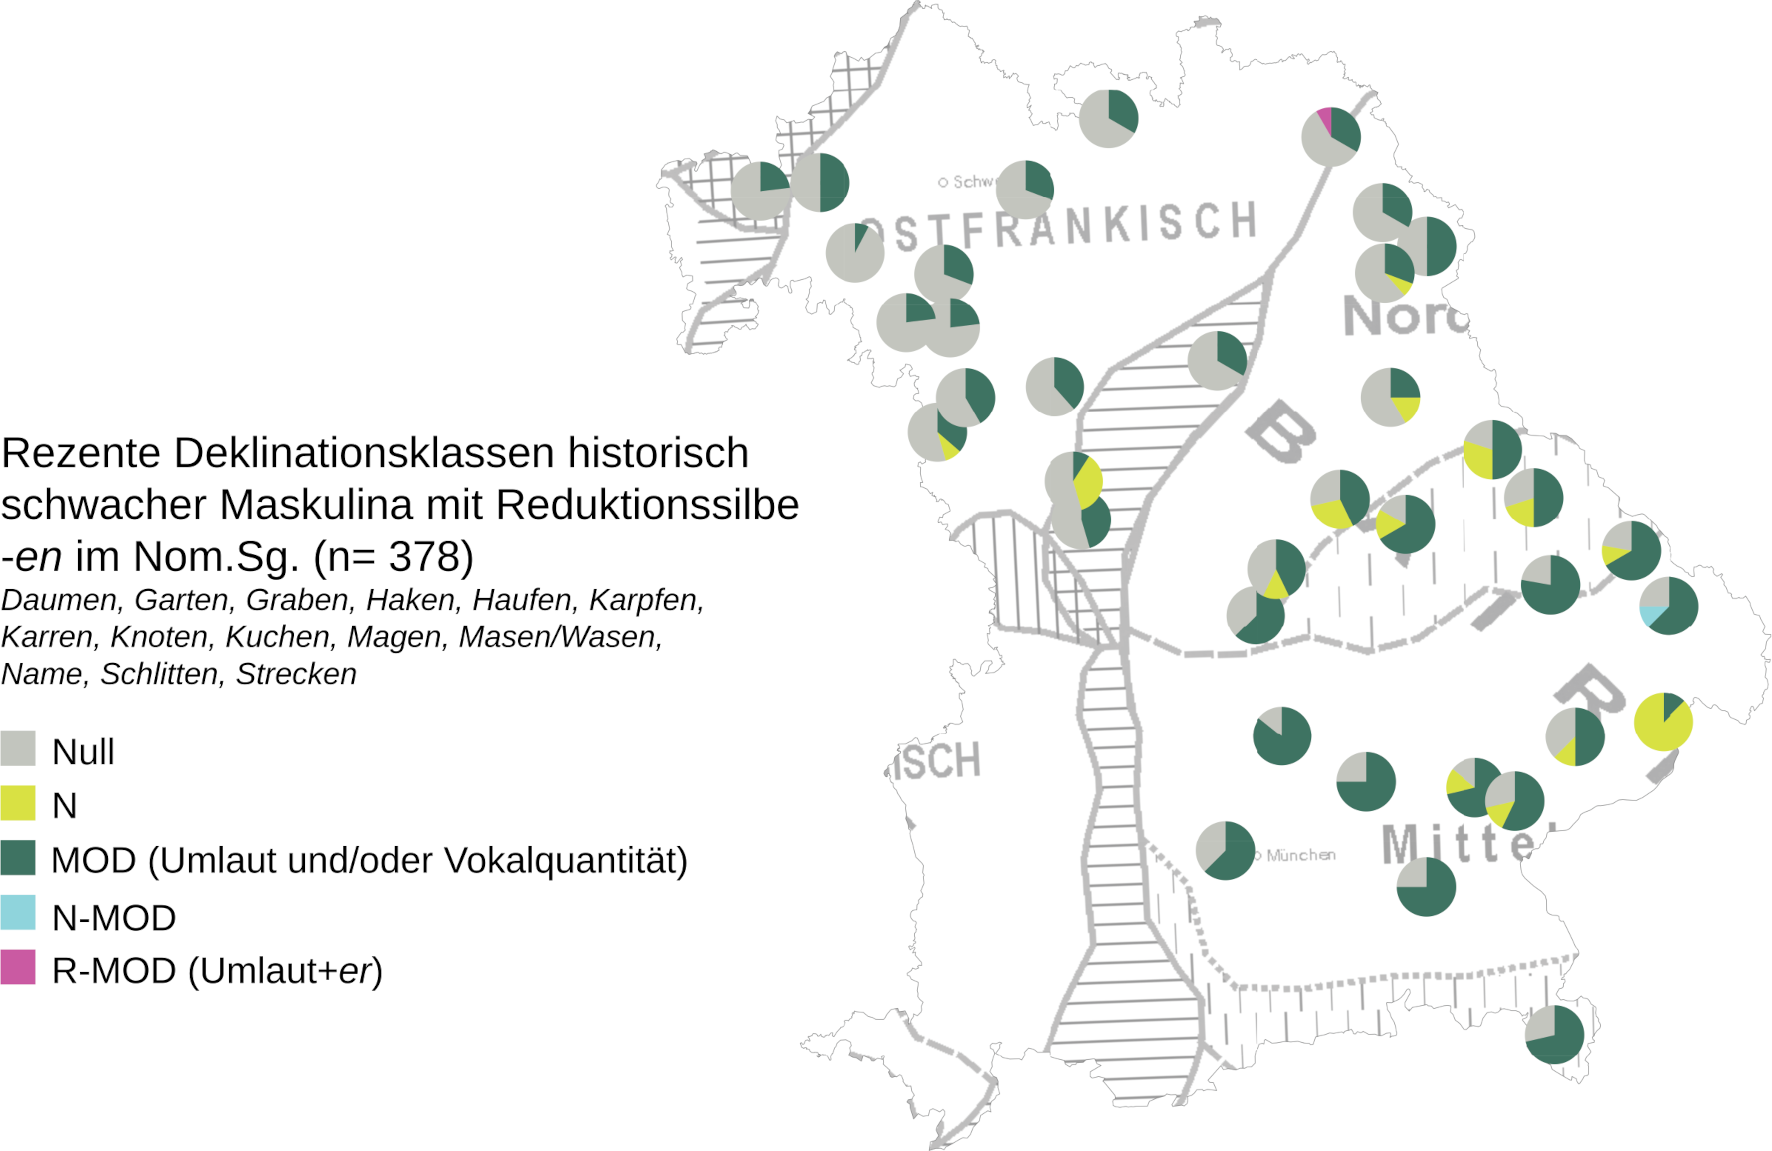
\includegraphics[width=\textwidth]{figures/Karte27.png}
\caption[Rezente Deklinationsklassen historisch schwacher Maskulina, die Reduktionssilbe{}-en im Nom.Sg. aufweisen ]{\label{bkm:Ref53827307}\hypertarget{Toc81223976}{}Rezente Deklinationsklassen historisch schwacher Maskulina, die Reduktionssilbe -\textit{en} im Nom.Sg. aufweisen}
\label{map:27}
\end{map}

\subsection{Neutra}\label{sec:8.2.2}
\begin{sloppypar}
Die Neutra der \textit{a}-Deklination weisen historisch Nullplural auf. Im Mittelhochdeutschen setzt ein Wechsel zur Deklination der historischen \textit{iz/az}{}-Klasse (UL+\textit{er}) oder zum Schwa-Suffix der Maskulina ein, im obd. Sprachraum hindert die Apokope jedoch die analoge Ausbreitung dieses Pluraltyps (vgl. \sectref{sec:3.1.2}). Während einige wenige Neutra (\textit{Fenster}, \textit{Haar}, \textit{Knie}) auch in den rezenten Dialekten im gesamten UG Nullplural aufweisen, sind bei anderen historischen \textit{a}{}-Neutra neben Nullplural auch Deklinationsklassenwechsel in das Pluralverfahren der historischen \textit{iz/az}{}-Klassen belegt (vgl. \citealt[§798]{Schmeller1821}). \textit{Schaf} etwa weist im UG Nullplural auf, nur im nördlichen Nordbair. wird der Plural additiv mit Tiefschwa gebildet (z.\,B. \teuthoo{s\#ôo.<o4v5}{š{\aufstrih}ôͅọv̩} -- \teuthoo{s\#ôo.<o4vA}{š{\aufstrih}ôͅọvα} im nordbair. Groschlattengrün). Im ofr. Erlabrunn (und in einigen weiteren der umgebenden unterofr. Ortsdialekte) findet sich daneben der analoge Umlautplural \teuthoo{s\#o.2Av5}{šōͅαv̩} -- \teuthoo{s\#a9.2v5}{ša\klammeruntenpost{}̄ͅv̩} ‚Schaf‘ (vgl. \citealt[Karte 50]{SBS9.1}). Der his\-to\-ri\-sche \textit{a}{}-Stamm \textit{Bein} ist im Ofr. (Typ \teuthoo{ba2}{bā} -- \teuthoo{di}{di} \teuthoo{ba2}{bā}), vereinzelt auch im Mittelbair. (Typ \teuthoo{boA}{boα} -- \teuthoo{boA}{boα}) mit Nullplural belegt, im Bair. finden sich dagegen Pluralformen mit Tiefschwa (Typ \teuthoo{boA}{boα} -- \teuthoo{boAnA}{boαnα}), im Nordbair. zudem mit dem umlautähnlichen Diphthongwechsel von mhd. \textit{ei} (z.\,B. \teuthoo{bo>+A+}{bỗα̃} -- \teuthoo{bo>+i6nA}{bỗĩnα} im nordbair. Tirschenreuth).\footnote{\citet[131]{Mauser2000} beobachtet in seiner Apparent-time-Studie im Salzburger Lungau Dialektwandel bei den neutralen \textit{a}{}- und \textit{ja}{}-Stämmen: Nullplural entspricht dabei der konservativeren Variante, die von der älteren Generation verwendet wird (z.\,B. \textit{b̥õɐ} -- \textit{b̥õɐ} ‚Bein‘, \textit{ˈhɒˑŋ} -- \textit{ˈhɒˑŋ} ‚Horn‘), während die jüngere Generation die innovativere, numerusdistinkte Varianten realisiere: Pl. \textit{ˈb̥õɐˑnɐ} ‚Beine‘, \textit{ˈhɛˑŋɐ} ‚Hörner‘.} Bei anderen Lexemen (\textit{Fest}, \textit{Seil}, \textit{Sieb}, \textit{Tor}) hat im UG weitgehend ein Wechsel in die Flexion der his\-to\-ri\-schen \textit{iz/az}{}-Klasse stattgefunden, Nullplurale finden sich nur vereinzelt und ohne Raumbildung (vgl. z.\,B. auch \citealt[Karte 14]{SMF7} oder \citealt[Karte 101]{SNiB7}).\footnote{Raumbildung gibt es indes bei der Realisierung des \textit{er}{}-Suffix als konsonantisches \textit{r}{}-Suffix, als Schwa oder Tiefschwa (vgl. \citealt[Karte 52]{SBS9.1}).} Ebenfalls ohne Raumbildung ist die Verteilung der rezenten Deklinationsklassen der historischen \textit{ja}-Stämme \textit{Bett}, \textit{Hemd}, \textit{(Ge-)Leise} und des \textit{a}{}-Stamms \textit{Kummet}, für die jeweils Nullplurale, Entsprechungen des \textit{er}{}-Suffixes und Nasalsuffix belegt sind.\footnote{Bei \textit{Kummet} findet sich einer der wenigen analogen Umlautplurale der Neutra, bezeichnenderweise geht dieser mit Genuswechsel zum Maskulinum einher: \teuthoo{dA}{dα} \teuthoo{k\_a.mAd}{kʰaͅmαd} -- \teuthoo{k\_a.mAd}{kʰaͅmαd} (mit velarisiertem Stammvokal mhd. {\textit{a}} {im Sg. und} hellem \textit{ạ}{}-Laut im Pl.{) im nordbair.-mittelbair. Blaibach.}}
\end{sloppypar}

Insgesamt muss für die Deklinationsklassenwechsel der historischen \textit{a}{}-Neutra diachron Variation und Dynamik angenommen werden, \citet[§798]{Schmeller1821} führt dieses Nebeneinander von Nullpluralen und (neueren) additiven Flexionsformen bei den Neutra auch für die damals rezenten Dialekte Bayerns an. Die diachrone Variation zeigen sowohl die oben aufgezeigten Varianten als auch die morphophonologischen Alternationen, die im UG bewahrt sind. Im Falle des his\-to\-ri\-schen \textit{a}{}-Stammes \textit{Kind} geht \citet[118]{Birkenes2014} davon aus, dass sich die Formen mit analogem \textit{er}{}-Suffix erst im Frühneuhochdeutschen durchgesetzt hat. Formen mit Schwa-Suffix waren \citet[119]{Birkenes2014} zufolge zum Ende des 13. Jahrhunderts im gesamten obd. Raum verbreitet, bedingt durch die einsetzende Apokope verschwinden diese Formen. In den rezenten ofr. und bair. Dialekten finden sich nur noch heteromorphische Varianten des \textit{er}{}-Suffixes. Dass das Schwa-Suffix his\-to\-risch im UG vorhanden war, zeigt synchron die subtraktive Pluralform \teuthoo{khe"+nd}{khẽ̄nd} -- \teuthoo{di}{di} \teuthoo{khen}{khen} im ofr.-hess. Wiesthal (vgl. \citealt[60--61]{Birkenes2014} zur Arealität der verschiedenen Pluralvarianten von \textit{Kind}). Daneben findet sich bei dem \textit{a}{}-Stamm \textit{Bein} neben additiven Formen auch die rein stammaffizierende Form \teuthoo{bo(+>A}{bỗ\klammerobenpost{}α} -- \teuthoo{bo(+>i.}{bỗ\klammerobenpost{}iͅ} im nordbair. Windischeschenbach, deren Diphthongwechsel auf eine historisch zweisilbige Pluralform mit apokopiertem Schwa-Suffix zurückgeht.\largerpage

Die Neutra der historischen \textit{iz/az}-Deklination markieren den Plural mit Umlaut und einer Variante des \textit{er}{}-Suffixes. Teilweise erfolgen daneben Kontraste der Vokalquantität und/oder von Lenis-Fortis-Obstruenten, z.\,B. \teuthoo{do2Av}{dōαv} -- \teuthoo{deEfA}{deəfα} ‚Dorf‘ im nordbair. Tirschenreuth. Innerparadigmatische Alternationen der Vokalqualität, die durch Ein- vs. Zweisilbigkeit der Wortform bedingt waren, führen bei Neutra, die historisch nur \textit{er}{}-Suffix aufwiesen, synchron zu einer Kombination aus \textit{er}{}-Suffix und Alternation der Vokalqualität: Alternationen der Zungenhöhe bei Stammvokal mhd. \textit{e} in Dehnung (z.\,B. \teuthoo{bri9."d}{bri\klammeruntenpost{}̄ͅd} -- \teuthoo{bre4dE}{brẹdə}. ‚Brett‘ im ofr. Burgbernheim) oder umlautähnlicher Diphthongwechsel bei mhd. \textit{ei} (z.\,B. \teuthoo{o\$A}{o̤α} -- \teuthoo{o.iA}{oͅiα} ‚Ei‘ im nordbair.-mittelbair. Bernhardswald).

Anders als im Neuhochdeutschen ist der Umlaut der rezenten Entsprechung der \textit{iz/az}{}-Klasse in den untersuchten Dialekten nicht grundsätzlich konkomitant, d.\,h. Umlaut wird nicht obligatorisch durch das \textit{er}{}-Suffix gefordert bzw. er tritt nicht automatisch ein (vgl. \citealt[82]{Dammel2018}, \citealt[163]{Rowley1997}).\footnote{Anders etwa \citet[§21]{Schübel1955} zum ofr. Dialekt von Stadtsteinach.} So finden sich bei dem his\-to\-ri\-schen \textit{iz/az}{}-Neutrum \textit{Maul} in den bair. Tiefenbohrungspunkten nur Formen ohne Umlaut: \teuthoo{ma24ý}{mạ̄ɫ} -- \teuthoo{ma42l.A}{mạ̄lͅα} (nordbair. Win\-disch\-eschen\-bach) oder -- mit vokalisiertem stammauslautendem /l/ -- \teuthoo{sma.e4}{smaͅẹ} -- \teuthoo{ma4eA}{mạeα} (nordbair.-mittelbair. Blaibach, vgl. \citealt[Karte 32]{SBS9.1}, \citealt[Karten 20, 38]{SMF2.1}). Auch wenn die Diminutivform in beiden Fällen keinen Umlaut aufweist (\teuthoo{ma24l.Adý@}{mạ̄lͅαdɫ̥} in Windischeschenbach, \teuthoo{ma.eAl}{maͅeαl} in Blaibach), so sind der Stammvokal mhd. \textit{û} und der Umlautvokal mhd. \textit{iu} -- anders als etwa die Vokalreihe mhd. \textit{ou}{}-\textit{öu}{}-\textit{ei} (z.\,B. \textit{Baum} -- \textit{Bäume}) -- im bair. Teil des UGs nicht systematisch zusammengefallen. Die Umlautlosigkeit ist im Falle von \textit{Maul} durch den folgenden Konsonanten /l/ bedingt. Vor bestimmten Velar- und Labialkonsonanten, \citet[9b, 49c]{Kranzmayer1956} nennt u.\,a auch /l/, ist der Umlaut bei mhd. \textit{û}, \textit{uo} und \textit{ou} ausgeblieben. Charakteristisch sei bei den umlautenhindernden Konsonanten „die starke Senkung der Hinterzunge“ (\citealt[49e]{Kranzmayer1956}), die die palatale Artikulation der Umlautprodukte behinderte. Der fehlende Umlaut bei \textit{Maul} ist damit schon im Mittelhochdeutschen und durch die phonotaktische Umgebung begründet (ausführlicher hierzu \sectref{sec:8.3.3.2}).\footnote{Der alte \textit{iz/az-}Stamm \textit{Haus} (ebenfalls mhd. \textit{û}) etwa wird in allen Tiefenbohrungspunkte durch UL+\textit{er} markiert (\teuthoo{ha4<o4s}{hậọs} -- \teuthoo{ha4<i.sA}{hậiͅsα} in Windischeschenbach, \teuthoo{A}{α} \teuthoo{ha.2s}{hāͅs} -- \teuthoo{he:2sA}{he{\doubleogonek}̄sα} in Blaibach).} Neben dem historischen \textit{iz/az}{}-Stamm \textit{Maul} finden sich auch bei den alten \textit{a}{}-Neutra \textit{Joch} und \textit{Tor} jeweils Varianten mit und ohne Umlaut, z.\,B. \teuthoo{to.<A}{tôͅα} -- \teuthoo{to.ArA}{toͅαrα} (nordbair.-mittelbair. Grafenkirchen) vs. \teuthoo{s\#do.2dl@do2A}{šdōͅdl̥dōα} -- \teuthoo{de2ArA}{dēαrα} (nordbair. Nabburg), \teuthoo{jo.x}{joͅx} -- \teuthoo{jo.HA}{joͅhͯα} (ofr. Pfofeld) vs. \teuthoo{jo9.x}{jo\klammeruntenpost{}ͅx} -- \teuthoo{jÔe.Xer}{j{\doppelaufstrih}eͅꭗer} (ofr. Gebsattel). Somit hat diachron eine (teilweise phonologisch bedingte) Reorganisation der \textit{iz/az}{}-Klasse stattgefunden, die sowohl die historischen Klassenmitglieder als auch die Klassenwechsler der neutr. \textit{a}{}-Deklination betrifft: in ein Pluralverfahren \textit{er}{}-Suffix, das auch Neutra mit velarem Stammvokal umfasst, und ein Verfahren \textit{er}{}-Suffix mit Alternation der Stammvokalqualität.

Die historisch schwachen Neutra der \textit{n}-Deklination \textit{Auge} und \textit{Ohr} markieren in den rezenten Dialekten den Plural mit Nasalsuffix, im Singularparadigma besteht weitestgehend Kasussynkretismus (vgl. \sectref{sec:7.2.2}, \citealt[88]{Rowley1997}). Deklinationsklassenwechsel in die NULL-Klasse liegt in den bair. Dialekten vor, wo das Nasalsuffix auch in den Nom.Sg. übertragen ist: \teuthoo{sqa2.N}{sʔāͅŋ} -- \teuthoo{a2.N}{āͅŋ} ‚Auge‘ (nordbair.-mittelbair. Blaibach), \teuthoo{s5o.A4n}{s̩oͅα̣n} -- \teuthoo{d5o.<A4n}{d̩oͅα̣n} ‚Ohr‘ (mittelbair. Grafenau, vgl. \citealt[426]{Rowley1990b}). Für eine kleine Gruppe von Neutra liegen Varianten der Pluralmarkierung mit Nasal- und \textit{er}{}-Suffix (ohne Raumbildung) vor: Die historischen \textit{ja}{}-Stämme \textit{Bett}, \textit{Hemd}, \textit{Leise} und der \textit{a}{}-Stamm \textit{Kummet} sind teilweise in die \textit{n}{}-Deklination, das historisch schwache Neutrum \textit{Herz} ist in einem Teil der untersuchten Ortsdialekte zum \textit{er}{}-Plural der historischen \textit{iz/az}{}-Deklination gewechselt.

\subsection{Feminina}\label{sec:8.2.3}
\begin{sloppypar}
Auch bei den starken Feminina der historischen \textit{i}-Deklination schwindet das Schwa-Suffix durch Apokope lautgesetzlich. Feminina dieser Deklination, die den Plural historisch durch UL+\textit{e} markieren, weisen in der Folge in den rezenten Dialekten rein stammaffizierende Pluralformen mit Umlaut auf, z.\,B. \teuthoo{gða.ns}{ɡ̩aͅns} -- \teuthoo{gðens}{ɡ̩ens} ‚Gans‘ (mittelbair. Kirchensur), \teuthoo{va\$osd}{va̤osd} -- \teuthoo{voesd}{voesd} ‚Faust‘ (ofr. Ahorn). Bei historisch kurzem Stammvokal in Dehnung in der einsilbigen Singularform und erhaltener Kürze in der zweisilbigen Pluralform erscheinen Kontraste der Vokalquantität (im Bair. in Kombination mit Lenis-Fortis-Kontrasten). Zum Teil, etwa im Falle von \textit{Faust} (mhd. \textit{û}), erscheinen analogische Quantitätskontraste: \teuthoo{va42o4sd}{vạ̄ọsd} -- \teuthoo{va43i.Sd}{vặiͅʃd} ‚Faust‘ (nordbair. Groschlattengrün), \teuthoo{go2ns}{ɡōns} -- \teuthoo{gðens5}{ɡ̩ens̩} ‚Gans‘ (ofr. Hallerstein). Lautgesetzlich entstanden sind ebenfalls die subtraktiven Pluralformen bei \textit{Hand} im ofr.-hess. Wiesthal und der umlautähnliche Diph\-thong\-wech\-sel von mhd. \textit{ei} bei \textit{Magd} im Nordbair. Im Ofr., wo mhd. \textit{ei} zu \teuthoo{a2}{ạ̄} oder \teuthoo{e2}{ē} monophthongiert ist und infolge der Apokope keine Numerusdistinktion vorliegt, wechselt \textit{Magd} in das Pluralverfahren mit Nasalsuffix (Typ \teuthoo{ma2d}{mād} -- \teuthoo{ma2dn}{mādn}, vgl. \mapref{map:17}). Bei den historischen \textit{i}{}-Stämmen \textit{Bank}, \textit{Hand}, \textit{Wand} ist der Umlaut in die Nominativ-Singular-Form eingedrungen, in der Folge erscheinen Numerussynkretismen (vgl. \sectref{sec:7.1.3.2}). Im bair. Teil des UGs erscheint bei \textit{Bank} und \textit{Wand} sekundäre Numerusdifferenzierung durch Nasalsuffix und damit Deklinationsklassenwechsel, z.\,B. \teuthoo{we+nt}{wẽnt} -- \teuthoo{dswoA}{dswoα} \teuthoo{we+ntn}{wẽntn} ‚Wand‘ im nordbair. Nabburg.
\end{sloppypar}

Ebenfalls in additive Klassen wechseln der historische \textit{i}{}-Stamm \textit{Naht} (Pl. mhd. \textit{næte}) sowie \textit{Nacht}, historisch ein fem. Wurzelstamm, der bereits im Althochdeutschen „spurenweise“ (\citealt[§241]{BrauneHeidermanns2018}) in die \textit{i}{}-Deklination wechselt (ahd. Nom./Akk.Pl. \textit{naht}, mhd. Pl. \textit{naht}, \textit{nehte} neben \textit{nahte}): \textit{Naht} in die N-Klasse (Typ \teuthoo{no2d}{nōd} -- \teuthoo{no2dn}{nōdn}), daneben ist für beide Feminina das kombinierte Verfahren UL+\textit{n} verbreitet, z.\,B. \teuthoo{na:2d5h}{na{\doubleogonek}̄d̩h} -- \teuthoo{ne.2dn}{nēͅdn} ‚Naht‘ im ofr. Wilhermsdorf, \teuthoo{no.xd5\_}{noͅxd̩ʰ} -- \teuthoo{na4X\textsuperscript{«d»}n}{nạꭗ\textsuperscript{d}n} ‚Nacht‘ im mittelbair. Waldhof. Die Pluralform \teuthoo{nôo(+u(+d5}{n{\aufstrih}õ\klammerobenpost{}ũ\klammerobenpost{}d̩} -- \teuthoo{nôo(+u(+nA}{n{\aufstrih}õ\klammerobenpost{}ũ\klammerobenpost{}nα} ‚Naht‘ im nordbair. Oberdolling belegt zudem, dass die spezifisch bair. Outputstruktur auf Nasal+Tiefschwa auch bei Feminina wirksam ist, die historisch (außer im Dat.Pl.) kein Nasalsuffix im Paradigma aufwiesen. Diese Form der Doppelsuffigierung findet sich auch bei dem \textit{i}{}-Stamm \textit{Tür} (\teuthoo{d5e}{d̩e} \teuthoo{d5i“4a}{d̩ị̄a} -- \teuthoo{d5i“4AnA}{d̩ị̄αnα} im mittelbair. Kirchensur), der im gesamten UG in additive Klassen (Nasalsuffix oder eine vokalische Variante) gewechselt ist. Damit erfolgt Deklinationsklassenwechsel in additive Verfahren bei den Feminina der historischen \textit{i}{}-Deklination bei lautgesetzlich oder morphologisch entstandenem Nullplural, aber auch, wie \textit{Nacht} und \textit{Naht} zeigen, bei velarem (d.\,h. umlautfähigem) Stammvokal und altem Umlautplural.

Historisch wiesen die Feminina der {\textit{n}}{{}-} und {\textit{ō}}{{}-Deklination} spezifische Paradigmenkonstellationen auf. Im Laufe des Frühneuhochdeutschen fusionieren beide Klassen zu einer Klasse, der fem. Mischdeklination (siehe 	\tabref{tab:10} und \sectref{sec:3.1.2}). In dieser Phase entsteht im Obd., insbesondere im Bair., ein regional begrenztes Ausgleichsmuster, indem das Nasalsuffix der historisch schwachen Feminina analog in den Nom.Sg. übertragen wird. Bei den fem. \textit{ō}{}-Stämmen, die historisch im Nominativ/Akkusativ Nullplural hatten, wird im Obd. das -\textit{(e)n}{}-Suffix des Gen./Dat.Pl. auf alle Kasus übertragen (vgl. \citealt[83]{KleinEtAl2018}). Diese beiden Paradigmenkonstellationen sind auch in den rezenten Dialekten des UGs zu finden und stellen eine Fortsetzung der historischen Deklinationsklassen dar. Die Singular- und Pluralformen der historischen \textit{ô}{}-Klasse entsprechen dem Typ \teuthoo{bruk}{bruk} -- \teuthoo{brukn}{brukn} ‚Brücke‘ mit apokopiertem Schwa im Singular, die historische \textit{n}{}-Klasse mit dem rezenten Typ \teuthoo{glokN}{ɡlokŋ} -- \teuthoo{glokN}{ɡlokŋ} ‚Glocke‘ weist Numerussynkretismus auf (\sectref{sec:7.1.3.1}, vgl. \citealt[§29.2]{Köhler1934}, \citealt[§35]{Schübel1955}). Eine Reorganisation der beiden Klassen findet dahingehend statt, dass für einzelne Feminina beide Paradigmenkonstellationen belegt sind, wie es exemplarisch das Beispiel \textit{Glocke} in 	\tabref{tab:39} mit den Flexionsmustern (1) und (2) illustriert.\footnote{\citet[§44]{Paul1968} gibt \textit{Glocke} als historisch schwach an, \citet{Lexer1872-1878} dagegen als schwankend.}


\begin{table}
\begin{tabular}{llll@{\,}c@{\,}llll@{\,}c@{\,}l|ll}
\lsptoprule
 & \multicolumn{2}{c}{\textit{n}-Klasse} &  &  & \multicolumn{3}{c}{Dialektale Klassen} &  &  & \multicolumn{2}{c}{\textit{ō}-Klasse} & \\
 \cmidrule(lr){2-3}\cmidrule(lr){6-8}\cmidrule(lr){11-12}
 & {Sg.} & {Pl.} &  & \textbf{${\rightarrow}$} &  & Sg. & Pl.  & \textbf{${\leftarrow}$} &  & \multicolumn{1}{l}{Sg.} & {Pl.} & \\
\midrule
N & \multicolumn{1}{l|}{\textit{zunge}} & \textit{zungen} & N &  & (1) & \teuthoo{glok}{ɡlok} & {\teuthoo{glokN}{ɡlokŋ}} &  & N & {\textit{gebe}} &  & N\\ \cline{2-2}
A &  &  & A &  & (2) & \teuthoo{glokN}{ɡlokŋ} & {\teuthoo{glokN}{ɡlokŋ}} &  & A &  &  & A\\ \cline{12-12}
G &  &  & G &  & \cellcolor{lsLightGray}(3) & \cellcolor{lsLightGray}\teuthoo{glokN}{ɡlokŋ} & \cellcolor{lsLightGray}{\teuthoo{gloknA}{ɡloknα}} &  & G &  & \textit{geben} & G\\
D &  &  & D &  & \cellcolor{lsLightGray}(4) & \cellcolor{lsLightGray}\teuthoo{glokN}{ɡlokŋ} & \cellcolor{lsLightGray}{\teuthoo{glokAn}{ɡlokαn}} &  & D &  &  & D\\
\lspbottomrule
\end{tabular}
\caption{Reorganisation der femininen \textit{n}{}- und \textit{ō}{}-Klasse bei historisch zweisilbiger Singularstammstruktur mit Schwa-Reduktionssilbe in den oobd. Dialekten am exemplarischen Beispiel \textit{Glocke}: Flexionsmuster (1) mit apokopiertem Singularstamm vs. (2) mit \textit{n}{}-erweitertem Singularstamm. Grau schattiert sind sekundäre, additive Pluralformen mit Tiefschwa-Suffix (3) oder Suffixalternation \textit{ŋ} > \textit{αn} (4).}
\label{tab:39}
\end{table}

Bei Feminina, die bereits im Mittelhochdeutschen zwischen \textit{n}{}- und \textit{ô}""-De"-kli"-na"-tion schwanken, stellen variierende Singularstammformen innerhalb eines Ortsdialekts, wie sie beispielsweise \citet[55]{White1966} für das westmittelbair. Eisenhofen angibt, die Fortsetzung der historischen Variation dar: \teuthoo{s\#dro.s}{šdroͅs} neben \teuthoo{s\#dro.sn}{šdroͅsn} -- \teuthoo{s\#dro.sn}{šdroͅsn} ‚Straße‘, \teuthoo{wis}{wis} neben \teuthoo{wisn}{wisn} -- \teuthoo{wisn}{wisn} ‚Wiese‘ (vgl. \citealt[§855]{Schmeller1821}, \citealt[§39a]{Schübel1955}, \citealt[117]{Zehetner1985}).

Daneben erklärt \citet[161]{Rowley1997} die „Konkurrenz“ zwischen Paradigmenkonstellationen (1) und (2) im Raum durch areal variierende Restrukturierungen der fem. Klassen. Demnach bildet das synkretische Paradigma (2) mit \textit{n}{}-erweiterter Singularform in einem nördlichen Streifen des Ofr. eine kleine, geschlossen Deklinationsklasse, während etwa im Bayerischen Wald zwar auch mehr Feminina nach (1) flektieren, das Flexionsmuster (2) aber „keineswegs als geschlossene Flexionsklasse bezeichnet werden kann“ (\citealt[161 und Karte 37]{Rowley1997}).\footnote{Auch nach \citet[15--16]{Mausser1915} sind die apokopierten Formen im Bayerischen Wald und in Teilen Oberbayerns („bis hart an die südbairische Grenze heran“) gebräuchlicher, die \textit{n}{}-erweiterten Formen fänden sich erst im niederbayrischen Flachland. \citet[17]{Mausser1915} führt neben arealer Variation in der Verwendung der beiden Formen auch vertikale Unterschiede an: Die zweisilbigen Formen auf -\textit{a} gälten zumindest in den Dialekten des Bayerischen Waldes als standardnäher, da sie eher der trochäischen Struktur der nhd. Feminina entsprechen.}  Einen weiteren Faktor, der diachron zu einer Reorganisation der Feminina der \textit{n}{}- und \textit{ô}{}-Deklination führt, stellen nach \citet{Rowley1997} semantische Merkmale dar. So flektieren Pflanzenbezeichnungen der historischen \textit{ô}{}-Klasse „weit verbreitet“ \citep[192]{Rowley1997} nach dem Paradigma (2) der schwachen Feminina, während Feminina beider historischer Klassen mit belebtem Denotat im nordbair. Egerland nach dem Muster (1) flektieren, nur Feminina mit dem Merkmal [$-$belebt] weisen im Nom.Sg. Nasalsuffix auf (vgl. \citealt[183]{HarnischRowley1990}). \citet[192]{Rowley1997} zufolge können zumindest die Ausnahmen von den Paradigmen (1) und (2) als direkte Entsprechungen der historischen Zugehörigkeit zur fem. \textit{ô}{}- respektive \textit{n}{}-Klasse durch diese semantischen Bereiche Pflanzen und Lebewesen erklärt werden (siehe auch \citealt[§850]{Schmeller1821}). Als Tendenz ergibt sich dies auch in den untersuchten Dialekten; so werden Baumbezeichnungen beider historischer Klassen weitestgehend mit \textit{n}{}-Erweiterung im Singular realisiert und das historisch schwache Femininum \textit{Katze} in allen Tiefenbohrungspunkten mit apokopiertem Schwa und distinkter Pluralform (Typ \teuthoo{katS}{katʃ} -- \teuthoo{katSn}{katʃn}).\footnote{Zu den Baumbezeichnungen gehören die historisch schwachen Feminina \textit{Birke}, \textit{Buche}, \textit{Erle} und \textit{Lärche} sowie der \textit{ô}{}-Stamm \textit{Eiche} und das im Mittelhochdeutschen schwankende Feminina \textit{Tanne}.}

\begin{sloppypar}
Von dieser Tendenz ausgenommen werden müssen aber einige mittelbair. Ortsdialekte sowie das mittelbair.-südbair. Ramsau, wo Baumbezeichnungen beider historischer Klassen mit apokopiertem Singularstamm realisiert werden (z.\,B. \teuthoo{b5u.Ax}{b̩uͅαx} -- \teuthoo{bu.<AxAn}{bûͅαxαn} ‚Buche‘, \teuthoo{o4a4X!}{ọạꭖ} -- \teuthoo{o4a4X!Y@}{ọạꭖ{\klammerNG}̥} ‚Eiche‘, \teuthoo{d\%a.<n}{d͈âͅn} -- \teuthoo{d\%a.nA}{d͈aͅnα} ‚Tanne‘ in Ramsau). Diese Beobachtung bestätigt sich insgesamt für jene Feminina, die \citet[§44]{Paul1968} oder \citet{Lexer1872-1878} als sicher schwach flektierend ausweisen: Im südlichen Mittelbair. und im mittelbair.-südbair. Übergangsgebiet werden diese mit apokopiertem Schwa und distinkter Pluralform nach dem Paradigma (1) realisiert (\mapref{map:28}). Hier scheint es eine Präferenz für apokopierte Singularstammformen unabhängig von der historischen Klassenzugehörigkeit zur fem. \textit{n}{}- oder \textit{ô}{}-Deklination zu geben, wie auch das Raumbild der \mapref{map:22} zur Singularstammform bei sämtlichen nhd. zweisilbigen Feminina im Korpus bestätigt.
\end{sloppypar}

\begin{map}
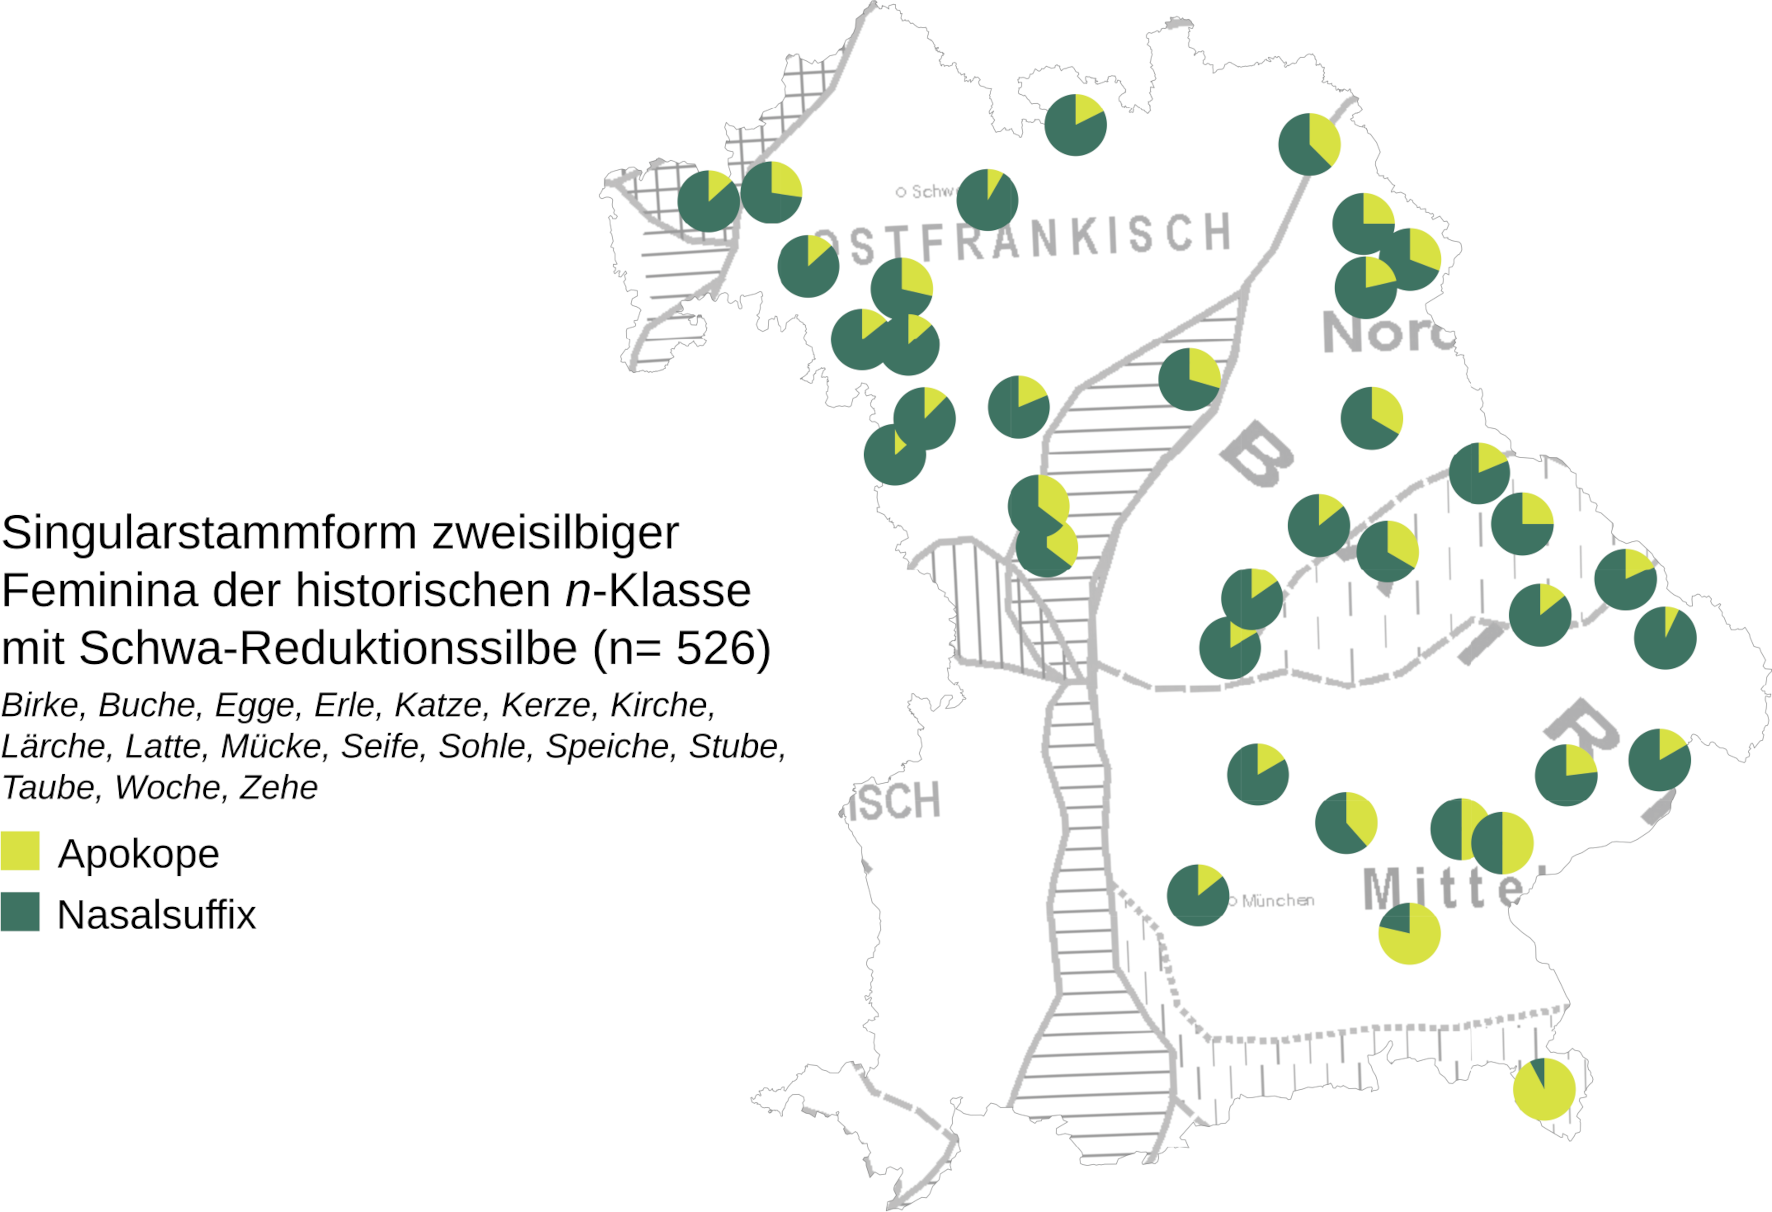
\includegraphics[width=\textwidth]{figures/Karte28.png}
\caption{Singularstammform historisch schwacher Feminina mit Schwa-Reduktionssilbe -- Häufigkeitsverteilung von Apokope vs. \textit{n}{}-Erweiterung im Nom.Sg.}
\label{map:28}
\end{map}

Eine (zumindest in einzelnen Dialekten wirksame) Reorganisation der his"-to"-ri"-schen \textit{n}{}- und \textit{ô}{}-Deklination erfolgt in den untersuchten Dialekten nicht nur im Bereich der Singularstammbildung, sondern auch mit Blick auf die Pluralmarkierung. \tabref{tab:39} weist für das Femininum \textit{Glocke} zwei numerusdistinkte Pluralformen bei \textit{n}{}-erweitertem Singularstamm aus: die additive Markierung mit Tiefschwa-Suffix in Typ (3), die bei vokalisch realisierter \textit{n}{}-Erweiterung als Nasalsuffix realisiert wird (Typ \teuthoo{biEkA}{biəkα} -- \teuthoo{biEkAn}{biəkαn} ‚Birke‘), sowie die Suffixalternation -\textit{n} > -\textit{αn} in Typ (4). Die graue Schattierung markiert, dass beide Verfahren dialektspezifisch für das Bair. sind.

Daneben erfolgt bei einigen Feminina ein Wechsel in die Umlautklasse: im Nordbair., vereinzelt im Ofr. und Mittelbair. \textit{Gabel} (Typ \teuthoo{go2wl}{ɡōwl} -- \teuthoo{ga2wl}{ɡāwl}) und \textit{Wurzel} vereinzelt im Nordbair. (Typ \teuthoo{wuAtS}{wuαtʃ} -- \teuthoo{wiEtS}{wiətʃ} neben \teuthoo{wuAtSl}{wuαtʃl} -- \teuthoo{wiEtSl}{wiətʃl}). Der analoge Umlaut von \textit{Wurzel} wie auch der historisch schwachen Feminina \textit{Mücke} und \textit{Stube}, des \textit{ô}{}-Stamms \textit{Furche} sowie von \textit{Brücke}, im Mittelhochdeutschen zwischen \textit{n}{}- und \textit{ô}{}-Deklination schwankend, ist dabei durch den Stammvokal bedingt. Der Umlaut des Kurzvokals mhd. \textit{u} in geschlossener Silbe ist im Obd. historisch unterblieben oder rückgängig gemacht worden, v.\,a. im nördlichen Oobd. bestand die Tendenz, die Umlautlosigkeit im Singular zu bewahren oder analogisch herzustellen (siehe \sectref{sec:7.1.2.1.1}). Diesen umlautlosen Singularformen stehen Pluralformen mit (analogem oder historischem) Umlaut gegenüber (vgl. 	\tabref{tab:20}). Mit Blick auf die Formenbildung ist interessant, dass reine Umlautplurale bei apokopiertem Singularstamm vor allem im Nordbair. zu finden sind, d.\,h. das Nasalsuffix des Ausgleichsparadigmas der historischen \textit{ô}{}-Deklination erscheint hier nicht: \teuthoo{b,ruk}{b͓ruk} -- \teuthoo{b,rik}{b͓rik} ‚Brücke‘ im nordbair. Nabburg, \teuthoo{vo.rc}{voͅrX} -- \teuthoo{vîirc}{v{\aufstrih}irX} ‚Furche‘ im nordbair.-ofr. Pfofeld, daneben auch analoge Umlautplurale bei \textit{Straße} des Typs \teuthoo{s\#5d5ro.S}{š̩d̩roͅʃ} -- \teuthoo{s\#5d5ra4S}{š̩d̩rạʃ} (mittelbair. Grafenau). Die Kombination aus Umlaut und Nasalsuffix (Typ \teuthoo{go2wl}{ɡōwl} -- \teuthoo{ga2wln}{ɡāwln} oder \teuthoo{s\#droS}{šdroʃ} -- \teuthoo{s\#draSn}{šdraʃn}) und aus Umlaut und Tiefschwa-Suffix (Typ \teuthoo{s\#du.m}{šduͅm} -- \teuthoo{s\#dI2mA}{šdı̄mα}) finden sich (wie auch bei zweisilbigen Maskulina der historischen \textit{i}{}-Deklination, vgl. \sectref{sec:8.2.1}) nur im bair. Teil des UGs (vgl. \citealt[§864]{Schmeller1821}).

Die Feminina der historischen \textit{r}-Klasse, die Verwandtschaftsbezeichnungen \textit{Mutter} und \textit{Tochter}, markieren im Mittelhochdeutschen den Plural mit Umlaut, \textit{Schwester} flektiert nach der fem. Mischdeklination, d.\,h. synkretisches Singularparadigma und Nasalsuffix im Plural (\citealt[§43]{Paul1968}). \textit{Mutter} weist vor allem im Ofr. Umlautplural auf, im bair. Teil des UGs ist der Wechsel in die schwache Flexion mit Nasalsuffix verbreitet (vgl. \citealt[Karte 131]{SNiB7}). Hier müssen zwei unterschiedliche Paradigmenkonstellation unterschieden werden: ein synkretisches Singularparadigma (Typ Sg. \teuthoo{mutA}{mutα} -- Pl. \teuthoo{mutAn}{mutαn}), das v.\,a. im Nordbair. und in Teilen des Ofr. vorkommt, und ein Singularparadigma mit distinkter Dativ-Singular-Form (Typ Nom./Akk.Sg. \teuthoo{mutA}{mutα} -- Dat.Sg. \teuthoo{mutAn}{mutαn} -- Pl. \teuthoo{mutAn}{mutαn}) im südlichen Nordbair. und in Teilen des Mittelbair. (vgl. \mapref{map:25} und \sectref{sec:7.2.2}). In diesem Teil des UGs flektieren \citet[137]{Rowley1997} zufolge auch \textit{Tochter} und \textit{Schwester} schwach (Dat.Sg. \teuthoo{s\#weStan}{šweʃtan}), es handelt sich um den semantisch konditionierten Klassenwechsel in die Deklinationsklasse der Verwandtschaftsbezeichnung, der auch bei den Maskulina stattgefunden hat (vgl. \sectref{sec:8.2.1}).

\textit{Schwester} ist in den BSA-Daten nur in der Nominativ-Singular- und Plural-Form belegt (die Pluralmarkierung erfolgt durch Nasalsuffix), doch zeigen die Wenker-Materialien, dass die schwache Dativ-Singular-Form in diesem Teil des Bair. weit verbreitet und auch in einzelnen Tiefenbohrungspunkte belegt ist, z.\,B. \textit{sag deiner Schwöstern} ‚sag Deiner Schwester‘ im mittelbair. Neukirchen am Inn (vgl. \citealt{WA}-Karte 249 „Schwester“). \textit{Tochter} weist im gesamte UG Umlautplural auf, nur im nordbair. Oberdolling (\teuthoo{do4<xd\%A}{dộxd͈α} -- \teuthoo{de?Xd\%An}{dëꭗd͈αn}) und im mittelbair. Grafenau (\teuthoo{d\%o9.uXtE}{d͈o\klammeruntenpost{}ͅuꭗtə} -- \teuthoo{te.ct;En}{teͅCt͓͓ən}) finden sich die kombinierten Markierungen aus Umlaut und Nasalsuffix, die auch \citet[137]{Rowley1997} für \textit{Tochter} neben \textit{Bruder} anführt; auch hier hat der Wechsel in die schwache Klasse „enge Verwandtschaft“ stattgefunden (vgl. \citealt[Karte 123]{SNiB7}). Die BSA-Daten deuten jedoch daraufhin, dass die schwache Flexion der Verwandtschaftsbezeichnung zum Teil bereits abgebaut ist: Die Gewährsperson im ofr. Hallerstein kennzeichnete die Form \teuthoo{di}{di} \teuthoo{mu.dAn}{muͅdαn} als ‚früher‘ und produzierte selber den Umlautplural \teuthoo{mi.dEr}{miͅdər}.

\section{Konditionierungsprinzipien der dialektalen Deklinationsklassen}\label{sec:8.3}
Die dialektalen Deklinationsklassensysteme werden im Folgenden im Hinblick auf die in \sectref{sec:3.2} eingeführten außerflexivischen Konditionierungsfaktoren analysiert. Ziel ist es zu zeigen, inwiefern Klassenzugehörigkeit und Deklinationsklassenwandel durch diese außerflexivischen Merkmale in den Dialekten konditioniert sind, welche Faktoren überhaupt wirksam sind und ob es dialektspezifische Konditionierungsprinzipien gibt. Da die Untersuchung auf vorhandenen Erhebungsdaten basiert und damit von deren Zusammensetzung abhängig ist, sind Aussagen zu allen bekannten Konditionierungsfaktoren nicht in der Tiefe möglich, wie sie wünschenswert wären (dies betrifft v.\,a. Derivationen und damit morphologische Konditionierung in \sectref{sec:8.3.4}). Gleichzeitig lassen die Daten der BSA-Erhebungen Rückschlüsse auf die Struktur und Zusammensetzung der dialektalen Deklinationsklassen zu. Bedingt durch die unterschiedlichen Forschungsziele der publizierten Sprachatlasbände wurden die Daten nie systematisch dahingehend ausgewertet.

\subsection{Genus}
\label{sec:8.3.1}
Im Standarddeutschen hat sich im Bereich der Pluralallomorphie und genusspezifischer Paradigmenausprägungen eine Schranke zwischen femininen und nicht-femininen Deklinationsklassen herausgebildet (vgl. \sectref{sec:4.1}). Diese Opposition ist das Ergebnis eines Umbaus des Deklinationsklassensystems im Laufe des Frühneuhochdeutschen, der einerseits die Reorganisation der Maskulina und Neutra der historischen \textit{i}{}- und \textit{a}{}-Deklination, anderseits die Herausbildung einer spezifisch fem. Mischdeklination und damit die Ablösung der ahd. Genusschranke zwischen Neutrum und Nicht-Neutrum umfasste (siehe \sectref{sec:3.1.2}). Die in \sectref{sec:8.2} aufgeführten Deklinationsklassenwechsel zeigen, dass sich Genus auch in den untersuchten Dialekten als ein zentraler Steuerungsfaktor der Deklinationsklassenzugehörigkeit erweist. Einzelne Wechselbewegungen und rezente Pluralformen sind allerdings nur in Kombination mit anderen Konditionierungsfaktoren zu erklären.


\begin{figure}
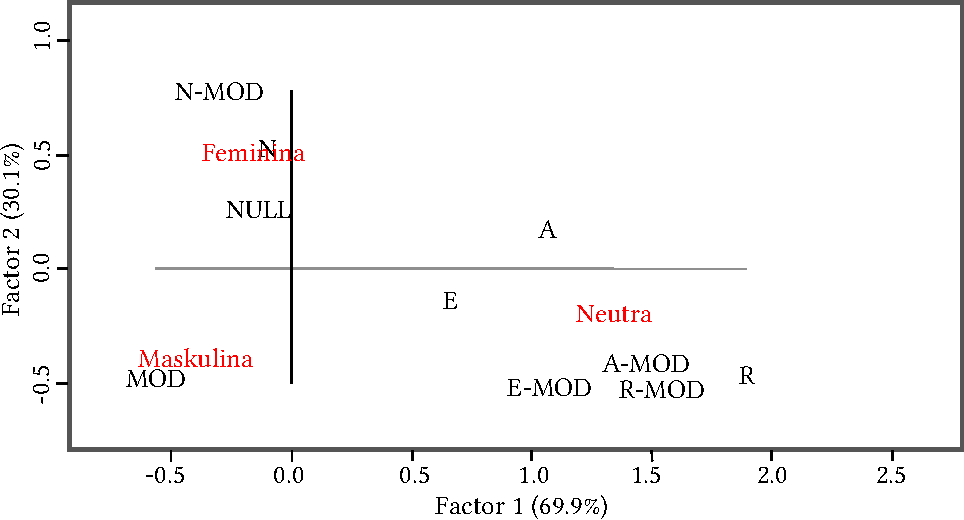
\includegraphics[width=\textwidth]{figures/revisedNickelNominalmorphologie-img044.pdf}
\caption{Korrespondenzanalyse der Variablen Genus und Deklinationsklasse in den untersuchten Dialekten ($n=7943$)}
\label{fig:13}
\end{figure}

\begin{table}
    \begin{tabular}{lrrr}
    \lsptoprule
         &  \multicolumn{3}{c}{Genus}\\
         \cmidrule(lr){2-4}
        DK & Feminina & Maskulina & Neutra\\
        \midrule
        NULL & 1414 & 948 & 316\\
        N & 843 & 312 & 131\\
        A & 159 & 20 & 231\\
        E & 39 & 42 & 63\\
        R & 1 & 4 & 63 \\
        N-MOD & 107 & 27 & 2\\
        A-MOD & 33 & 73 & 348\\
        E-MOD & 9 & 51 & 100\\
        R-MOD & 3 & 33 & 146\\
        MOD & 499 & 1916 & 10\\
        \midrule
        gesamt & 3107 & 3426 & 1410\\
        \lspbottomrule
    \end{tabular}
    \caption{Korrespondenzanalyse der Variablen Genus und Deklinationsklasse in den untersuchten Dialekten ($n=7943$)}
    \label{tabfig:13}
\end{table}

Inwiefern steuert Genus die Pluralallomorphie in den untersuchten Dialekten, inwiefern sind Deklinationsklassen genusspezifisch?  \figref{fig:13} und \tabref{tabfig:13} visualisiert die Häufigkeitsverteilung der Variablen Genus und Deklinationsklasse in Form einer Korrespondenzanalyse mit absoluten Häufigkeiten für das gesamte BSA-Korpus und unter Ausblendung der arealen Dimension.\footnote{Siehe einführend \sectref{sec:7.1.2.3.1} zur Methodik der Korrespondenzanalyse.}  Im relativen Vergleich zeigen die Entfernungen zwischen den einzelnen Variablenausprägungen, dass es Deklinationsklassen gibt, die mit einzelnen Genera korrelieren. Bei Klassen mit additiven Allomorphen ist jeweils die Heteromorph-Ebene beibehalten, d.\,h. Schwa-, Tiefschwa- und \textit{er}{}-Suffix wurden nicht als Heteromorphe des \textit{er}{}-Suffixes, und Schwa-, Tiefschwa- und Nasalsuffix nicht als Heteromorphe des \textit{en}{}-Suffixes abstrahiert. Die relative Entfernung zwischen den einzelnen Variablen auf der rechten Seite der horizontalen Achse weist die R-Klasse und die kombinierten Klassen E-, A- und R-MOD als spezifisch neutrale Klassen aus. Schwa- und Tiefschwa-Suffix (E- und A-Klasse) sind dagegen weniger stark mit den Neutra korreliert, da sie als heteromorphische Varianten des \textit{en}{}- und des \textit{er}{}-Suffixes in den untersuchten Dialekten distribuiert sind, und vokalisch realisierte \textit{en}{}-Plurale auch bei Feminina und Maskulina zu finden sind, etwa bei den \textit{n}{}-erweiterten Feminina (z.\,B. \teuthoo{v5loi).N}{v̩loi\klammeruntenpost{}ͅŋ} -- \teuthoo{vlo<iNA}{vlôiŋα} ‚Fliege‘ im mittelbair. Neukirchen am Inn) oder bei den Maskulina der historisch schwachen Deklination (z.\,B. \teuthoo{ogs5}{oɡs̩} -- \teuthoo{di}{di} \teuthoo{o4gsE}{ọɡsə} ‚Ochse‘ im ofr. Gemünden am Main).

Die linke Seite der horizontalen Achse ist durch Feminina und Maskulina bestimmt, allerdings ist die relative Entfernung beider Genera zueinander weniger groß als zu den Neutra. Auch hier sind einzelne Deklinationsklassen überaus häufig mit den beiden Genera korreliert: die MOD-Klasse mit den Maskulina, N- und NULL-Klasse mit den Feminina. Damit ergibt sich in der Tendenz für das BSA-Korpus insgesamt eine Genusschranke zwischen Neutrum und Nicht-Neutrum. Reduziert man die Datenauswertung von den Heteromorphen, die dialektübergreifend im gesamten UG zu finden sind, auf die Allomorphebene der einzelnen dialektalen Flexionssysteme, so ergeben sich variierende, ortsdialektspezifische Genuskonstellationen zwischen Ofr. und nördlichen Nordbair. einerseits und andererseits den Dialekten des südlichen Nordbair. und Mittelbair. Die Konstellationen, die in  \figref{fig:14a}--\ref{fig:14b} und \tabref{tabfig:14a}--\ref{tabfig:14b} für zwei exemplarische Ortsdialekte gezeigt werden, sind durch einen systematischen Unterschied im Suffixinventar begründet: Werden mhd. -\textit{en} und mhd. -\textit{er} auch im rezenten Flexionssystem unterschieden oder sind mhd. -\textit{en} und mhd. -\textit{er} in Folge der Vokalisierung von mhd. -\textit{en} in bestimmten phonologischen Kontexten zusammengefallen (ausführlicher hierzu \sectref{sec:7.1.1.1})?

Im ofr. Ahorn gibt es zwei additive Allomorphe: Schwa-Suffix als rezente Entsprechung der Reduktionssilbe mhd. -\textit{er} und Nasalsuffix für mhd. -\textit{en}, d.\,h. \textit{er}{}- und \textit{en}{}-Plural werden in diesem Flexionssystem auch synchron unterschieden. Die Streuung der Variablenausprägungen und die relative Entfernung im Plot der Korrespondenzanalyse zeigen wiederum die oben beobachtete Tendenz einer Opposition zwischen Neutrum und Nicht-Neutrum. NULL- und N-Klasse korrelieren überaus häufig mit Feminina, die MOD-Klasse mit den Maskulina und die Klassen E und E-MOD mit den Neutra. Diesen Befund bestätigt auch das Mosaik-Plot, das die Häufigkeitsverteilung der beiden Variablen visualisiert (die Größe der Flächen der Rechtecke ist relativ zur absoluten Häufigkeit zu lesen). N- und NULL-Klasse haben bei den Neutra nur eine periphere Bedeutung, die MOD-Klasse ist nicht vertreten.

In den bair. Dialekten ergibt sich eine andere Distribution von Deklinationsklassen und Genera, da Tiefschwa-Suffix (A-Klasse) als Vokalisierung des \textit{er}{}-Suffixes und als phonotaktisch bedingte vokalische Realisierung von mhd. -\textit{en} „tiefenstrukturell mehrdeutig“ \citep[127]{Rowley1997} ist. Im exemplarisch gewählten Dialekt von Bernhardswald, Übergangsgebiet zwischen südlichem Nordbair. und Mittelbair., weisen die relativen Entfernungen im Korrespondenzanalyse-Plot die
Klassen A-MOD als spezifisch für Neutra und MOD als spezifisch für Maskulina aus. Bemerkenswert ist, dass die Klassen N, NULL und N-MOD zwar stärker mit Femininum korrelieren (und, wie das Mosaik-Plot zeigt, diese in den Klassen auch anteilig am stärksten sind); doch grundsätzlich ist Femininum in allen Deklinationsklassen vertreten.

\begin{figure}
\begin{subfigure}{\textwidth}
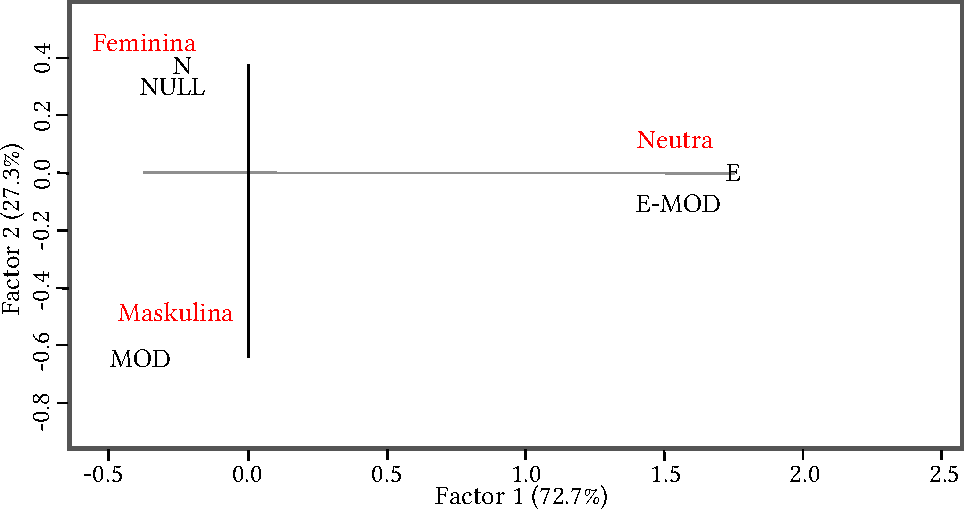
\includegraphics[width=\textwidth]{figures/revisedNickelNominalmorphologie-img045a.pdf}
\caption{}
\label{fig:14a-1}
\end{subfigure}
\begin{subfigure}{\textwidth}
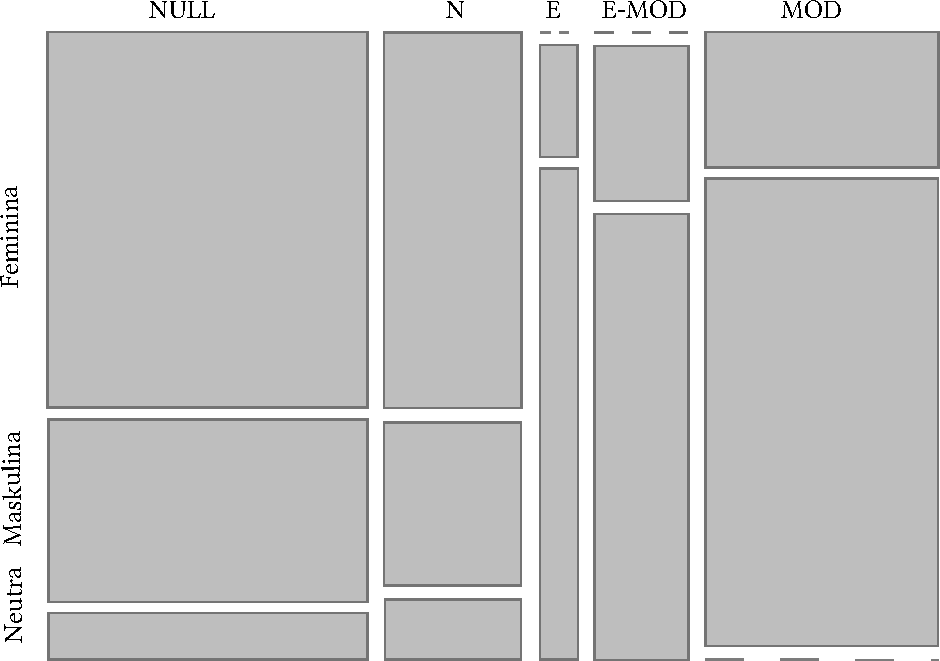
\includegraphics[width=\textwidth]{figures/revisedNickelNominalmorphologie-img045b.pdf}
\caption{}
\label{fig:14a-2}
\end{subfigure}
\caption{Korrespondenzanalyse und Mosaik-Plot der Variablen Genus und Deklinationsklasse in ofr. Ahorn ($n = 239$)}
\label{fig:14a}
\end{figure}

\begin{table}
    \begin{tabular}{lrrr}
    \lsptoprule
         & \multicolumn{3}{c}{Genus} \\
         \cmidrule(lr){2-4}
        DK & Feminina & Maskulina & Neutra\\
        \midrule
        NULL & 58 & 28 & 7\\
        N & 25 & 11 & 4 \\
        E & 0 & 2 & 9 \\
        E-MOD & 0 & 7 & 20\\
        MOD & 15 & 53 & 0\\
        \lspbottomrule
    \end{tabular}
    \caption{Tabelle der Variablen Genus und Deklinationsklasse in ofr. Ahorn ($n = 239$)}
    \label{tabfig:14a}
\end{table}

\begin{figure}
\begin{subfigure}{\textwidth}
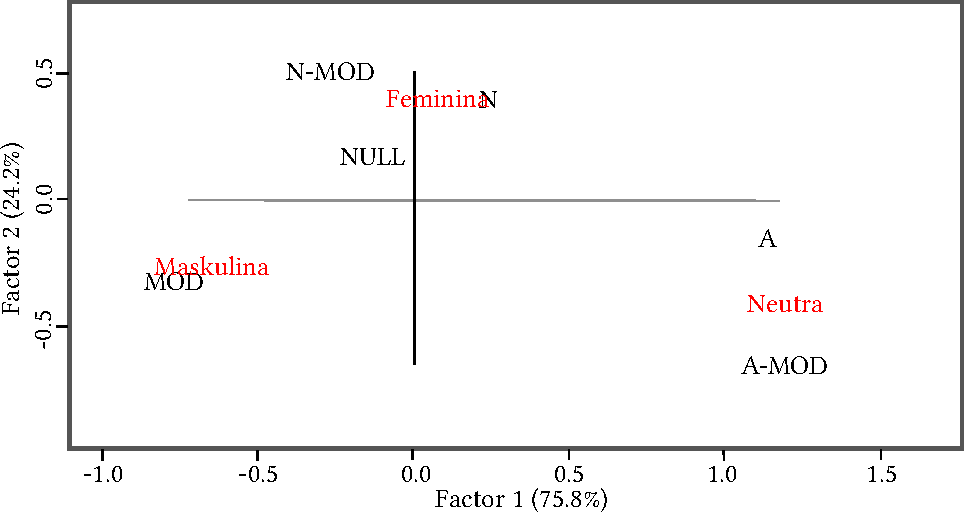
\includegraphics[width=\textwidth]{figures/revisedNickelNominalmorphologie-img045c.pdf}
\caption{}
\label{fig:14b-1}
\end{subfigure}
\begin{subfigure}{\textwidth}
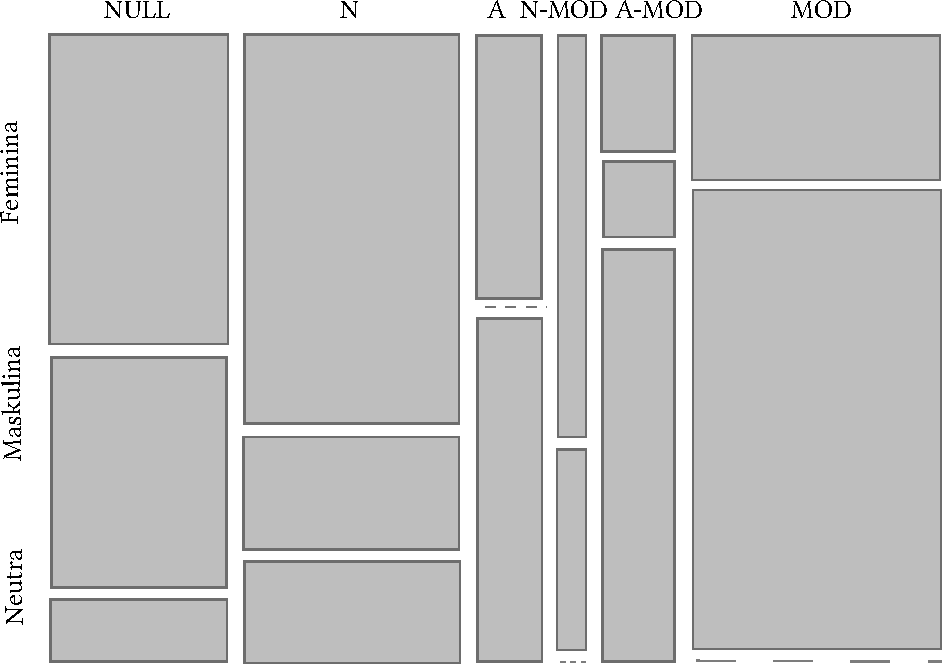
\includegraphics[width=\textwidth]{figures/revisedNickelNominalmorphologie-img045d.pdf}
\caption{}
\label{fig:14b-2}
\end{subfigure}
\caption{Korrespondenzanalyse und Mosaik-Plot der Variablen Genus und Deklinationsklasse in nordbair-mittelbair. Bernhardwald ($n = 178$)}
\label{fig:14b}
\end{figure}

\begin{table}
    \begin{tabular}{lrrr}
    \lsptoprule
         & \multicolumn{3}{c}{Genus} \\
         \cmidrule(lr){2-4}
        DK & Feminina & Maskulina & Neutra\\
        \midrule
        NULL & 20 & 15 & 4\\
        N & 31 & 9 & 8 \\
        A & 6 & 0 & 8 \\
        N-MOD & 4 & 2 & 0\\
        A-MOD & 3 & 2 & 11\\
        MOD & 13 & 42 & 0\\
        \lspbottomrule
    \end{tabular}
    \caption{Tabelle der Variablen Genus und Deklinationsklasse in nordbair-mittelbair. Bernhardwald ($n = 178$)}
    \label{tabfig:14b}
\end{table}

Im Deklinationsklassensystem ergibt sich damit keine eindeutige Opposition zwischen den Genera. Feminina markieren den Plural additiv mit Nasal- und Tiefschwa-Suffix, sodass sie als eine Art Verbindungsglied zwischen dem Nasalsuffix der Maskulina und dem Tiefschwa-Suffix der Neutra stehen. Die Distribution von Nasal- und Tiefschwa-Suffix bei den Feminina und des Nasalsuffixes bei Maskulina und Neutra ist durch dialektspezifische prosodisch-phonotaktische Konditionierungsbedingungen zu erklären (ausführlicher hierzu \sectref{sec:8.3.3}). In diesem bair. Ortsdialekt hat somit eine stärkere Formalisierung der Konditionierung diachron zur Schwächung einer Genusopposition geführt.

Im Folgenden wird die Distribution der Deklinationsklassen für die einzelnen Genera noch einmal zusammengefasst und die dialektspezifische Entwicklung der Feminina als Detailanalyse aufgezeigt.

\subsubsection{Maskulina}
\label{sec:8.3.1.1}
Dialektübergreifend stellen stammaffizierende Verfahren das frequenteste Mittel zur Pluralmarkierung bei den Maskulina dar, die MOD-Klasse ist damit die typenfrequenziell größte Klasse der Maskulina. Stammaffizierende Markierung erscheint als Umlaut bei den Maskulina der historischen \textit{i}{}-Deklination, als analoger Umlaut bei Klassenwechslern (etwa aus der historischen \textit{a}{}-Klasse) und in Form von lautgesetzlich entstanden Kontrasten der Vokalquantität und -qualität und des Konsonantismus oder als Kombination dieser Verfahren (vgl. \sectref{sec:8.2.1}). Infolge der Öffnung des UL+\textit{er}{}-Verfahrens der neutralen \textit{iz/az}{}-Klasse für Maskulina erscheint Umlaut bei einzelnen Lexemen in Kombination mit einer heteromorphischen Variante des \textit{er}{}-Suffixes (z.\,B. bei \textit{Dorn}, \textit{Halm}, \textit{Wurm}).

Nullplural findet sich bei einsilbigen, vor allem aber bei zweisilbigen Stämmen auf -\textit{en}, -\textit{el}, -\textit{er}. Hier sind jene Dialekte des südlichen Nordbair. und Mittelbair. ausgenommen, in denen eine prosodisch-phonotaktische Inputkonditionierung die additive Pluralmarkierung durch Nasalsuffix bedingt: ofr. \teuthoo{s\#liSl@}{šliʃl̥} -- \teuthoo{s\#liSl@}{šliʃl̥} vs. bair. \teuthoo{s\#liSl@}{šliʃl̥} -- \teuthoo{s\#liSl@n}{šliʃl̥n} ‚Schlüssel‘ (ausführlicher hierzu \sectref{sec:8.3.3.1}). Während die Nasalsuffigierung in diesen Fällen durch formale Konditionierung gesteuert ist, sind die übrigen Mitglieder der N-Klasse historisch schwache Maskulina (darunter \textit{Bauer}, \textit{Hase}, \textit{Ochse}). Teilweise, vor allem in den nordbair. Dialekten, finden sich zudem Klassenwechsler mit dem semantischen Merkmal [+belebt] (siehe \sectref{sec:8.3.2.2}). Wiederum im bair. Teil des UGs sind vereinzelt auch Maskulina in der A-Klasse vertreten, etwa \teuthoo{s\#doA}{šdoα} -- \teuthoo{s\#doAnA}{šdoαnα} ‚Stein‘ oder \teuthoo{bou}{bou} -- \teuthoo{boumA}{boumα} ‚Bube‘; die Suffigierung mit Tiefschwa in der Abfolge Nasal+α entspricht hier einer präferierten, dialektspezifischen prosodischen Outputstruktur des Bair.

\subsubsection{Neutra}
\label{sec:8.3.1.2}
Als spezifische Klassen der Neutra erweisen sich dialektübergreifend die rezenten Entsprechungen der historischen \textit{iz/az-}Deklination, R und R-MOD (bzw. deren heteromorphische Varianten), sie stellen die typenfrequentesten Klassen der Neutra dar. Diachron hat eine (zum Teil phonologisch bedingte) Reorganisation der \textit{iz/az}{}-Klasse stattgefunden, in der Folge ist der Umlaut bei \textit{er}{}-Suffigierung bei historischen \textit{iz/az}{}-Neutra und Klassenwechslern nicht grundsätzlich konkomitant (vgl. \sectref{sec:8.2.2}). Auch \citet[163]{Rowley1997} beobachtet „den Ansatz einer Verselbständigung“ des \textit{er}{}-Plurals ohne Umlaut in seinem nordostbayerischen UG. Als weitere additive Klasse ist die N-Klasse bei den wenigen historisch schwachen Neutra (\textit{Auge}, \textit{Ohr}, \textit{Herz}) sowie teilweise bei den alten \textit{a}{}- und \textit{ja}{}-Stämmen \textit{Bett}, \textit{Hemd}, \textit{Leise}, \textit{Kummet} belegt. Daneben weisen die zweisilbigen Diminutiva auf \textit{el}{}-Reduktionssilbe der prosodisch-phonotaktischen Inputkonditionierung entsprechend im südlichen Nordbair. und vereinzelt im Mittelbair. Nasalsuffix auf, daneben auch die Diminutiva mit Derivationssuffix -\teuthoo{XE}{ꭗə} im ofr.-hess. Wiesthal (siehe \sectref{sec:8.3.3.1} sowie \sectref{sec:8.3.4} zur morphologischen Konditionierung). Nullplural weisen hingegen nur einige historische \textit{a}{}-Stämme auf (\textit{Fenster}, \textit{Haar}, \textit{Knie}, teilweise \textit{Schaf}) sowie die historischen \textit{n}{}-Stämme \textit{Auge} und \textit{Ohr} mit Nasalsuffix im Nom.Sg. im Bair. (vgl. \sectref{sec:8.3.2.1}).

\subsubsection{Feminina}
\label{sec:8.3.1.3}
Im gesamten UG weisen die historischen \textit{i}{}-Stämme auch in den rezenten Dialekten stammaffizierende Markierung auf, zudem sind einige analoge Umlautplurale in der MOD-Klasse zu finden, etwa bei \textit{Gabel}, \textit{Mücke} oder \textit{Straße} (siehe \sectref{sec:8.2.3}). Im bair. Teil des UGs erscheinen alte und analoge Umlautplurale in Kombination mit Nasalsuffix (Klasse N-MOD), und zwar sowohl bei einsilbigem (häufig apokopiertem) Singularstamm oder bei zweisilbigen Stämmen.

Eine Zweiteilung des UGs ergibt sich bei der typenfrequenten Klasse der his\-to\-ri\-schen \textit{n}{}- und \textit{ô}{}-Stämme, die in den rezenten Dialekten mit apokopierter Singularform oder mit Nasalsuffix im Nom.Sg. realisiert werden. Im gesamten UG markieren apokopierte Stämme den Plural regelmäßig mit Nasalsuffix (d.\,h. N-Klasse); ausgenommen werden müssen hier apokopierte Feminina mit kollektiver Semantik (etwa \textit{Bremse}, \textit{Birne}, \textit{Kirsche}, \textit{Klaue}), die dialektübergreifend, vor allem aber im südlichen Nordbair., häufig Nullplural aufweisen (Typ \teuthoo{erwEs}{erwəs}-- \teuthoo{erwEs}{erwəs} ‚Erbse‘, ausführlicher hierzu \sectref{sec:8.3.2.1}). Eine dialektraumspezifische Form der Pluralmarkierung findet sich indes bei den Feminina mit \textit{n}{}-Erweiterung. Hier liegt auch die Lösung begründet für die eingangs beobachtete variierende Genuskonstellation zwischen den Dialekten des südlichen Nordbair. und des Mittelbair. sowie dem Ofr. und nördlichen Nordbair.

In \mapref{map:29} ist die absolute Häufigkeit der numerussynkretischen NULL-Klas\-se (links) und der numerusdistinkten Klassen N und A (rechts) bei \textit{n}{}-erweiterten Feminina gegenübergestellt. Differenziert wurde zudem die Form der Reduktionssilbe (Nasal vs. vokalische Realisierung des Nasalsuffixes). Die Raumbildung zeigt, dass die additive Markierung der \textit{n}{}-erweiterten Feminina sowohl nach Nasal- als auch nach Tiefschwa-Suffix ein Spezifikum des südlichen Nordbair. und des Mittelbair. ist.\footnote{Vgl. hierzu auch die Raumbildung von \citealt{WA}-Karte 72 „Wochen“. Bemerkenswert ist hier, dass die distinkte Pluralform im Abfragekontext des Wenker-Satzes nach einer Zahlenangabe erfolgt, wo sie in den untersuchten Dialekten regelmäßig unterbleibt, beispielsweise im nordbair.-mittelbair. Zwiesel: \textit{Er is vor vie oder fünf Wochan gstoam} ‚Er ist vor vier oder fünf Wochen gestorben‘ (vgl. \sectref{sec:8.3.2}).} Zwar weisen auch die Dialekte des westlichen Ofr. vokalisierte Reduktionssilben auf, doch erscheint hier eine additive Markierung nicht systematisch.

\begin{map}
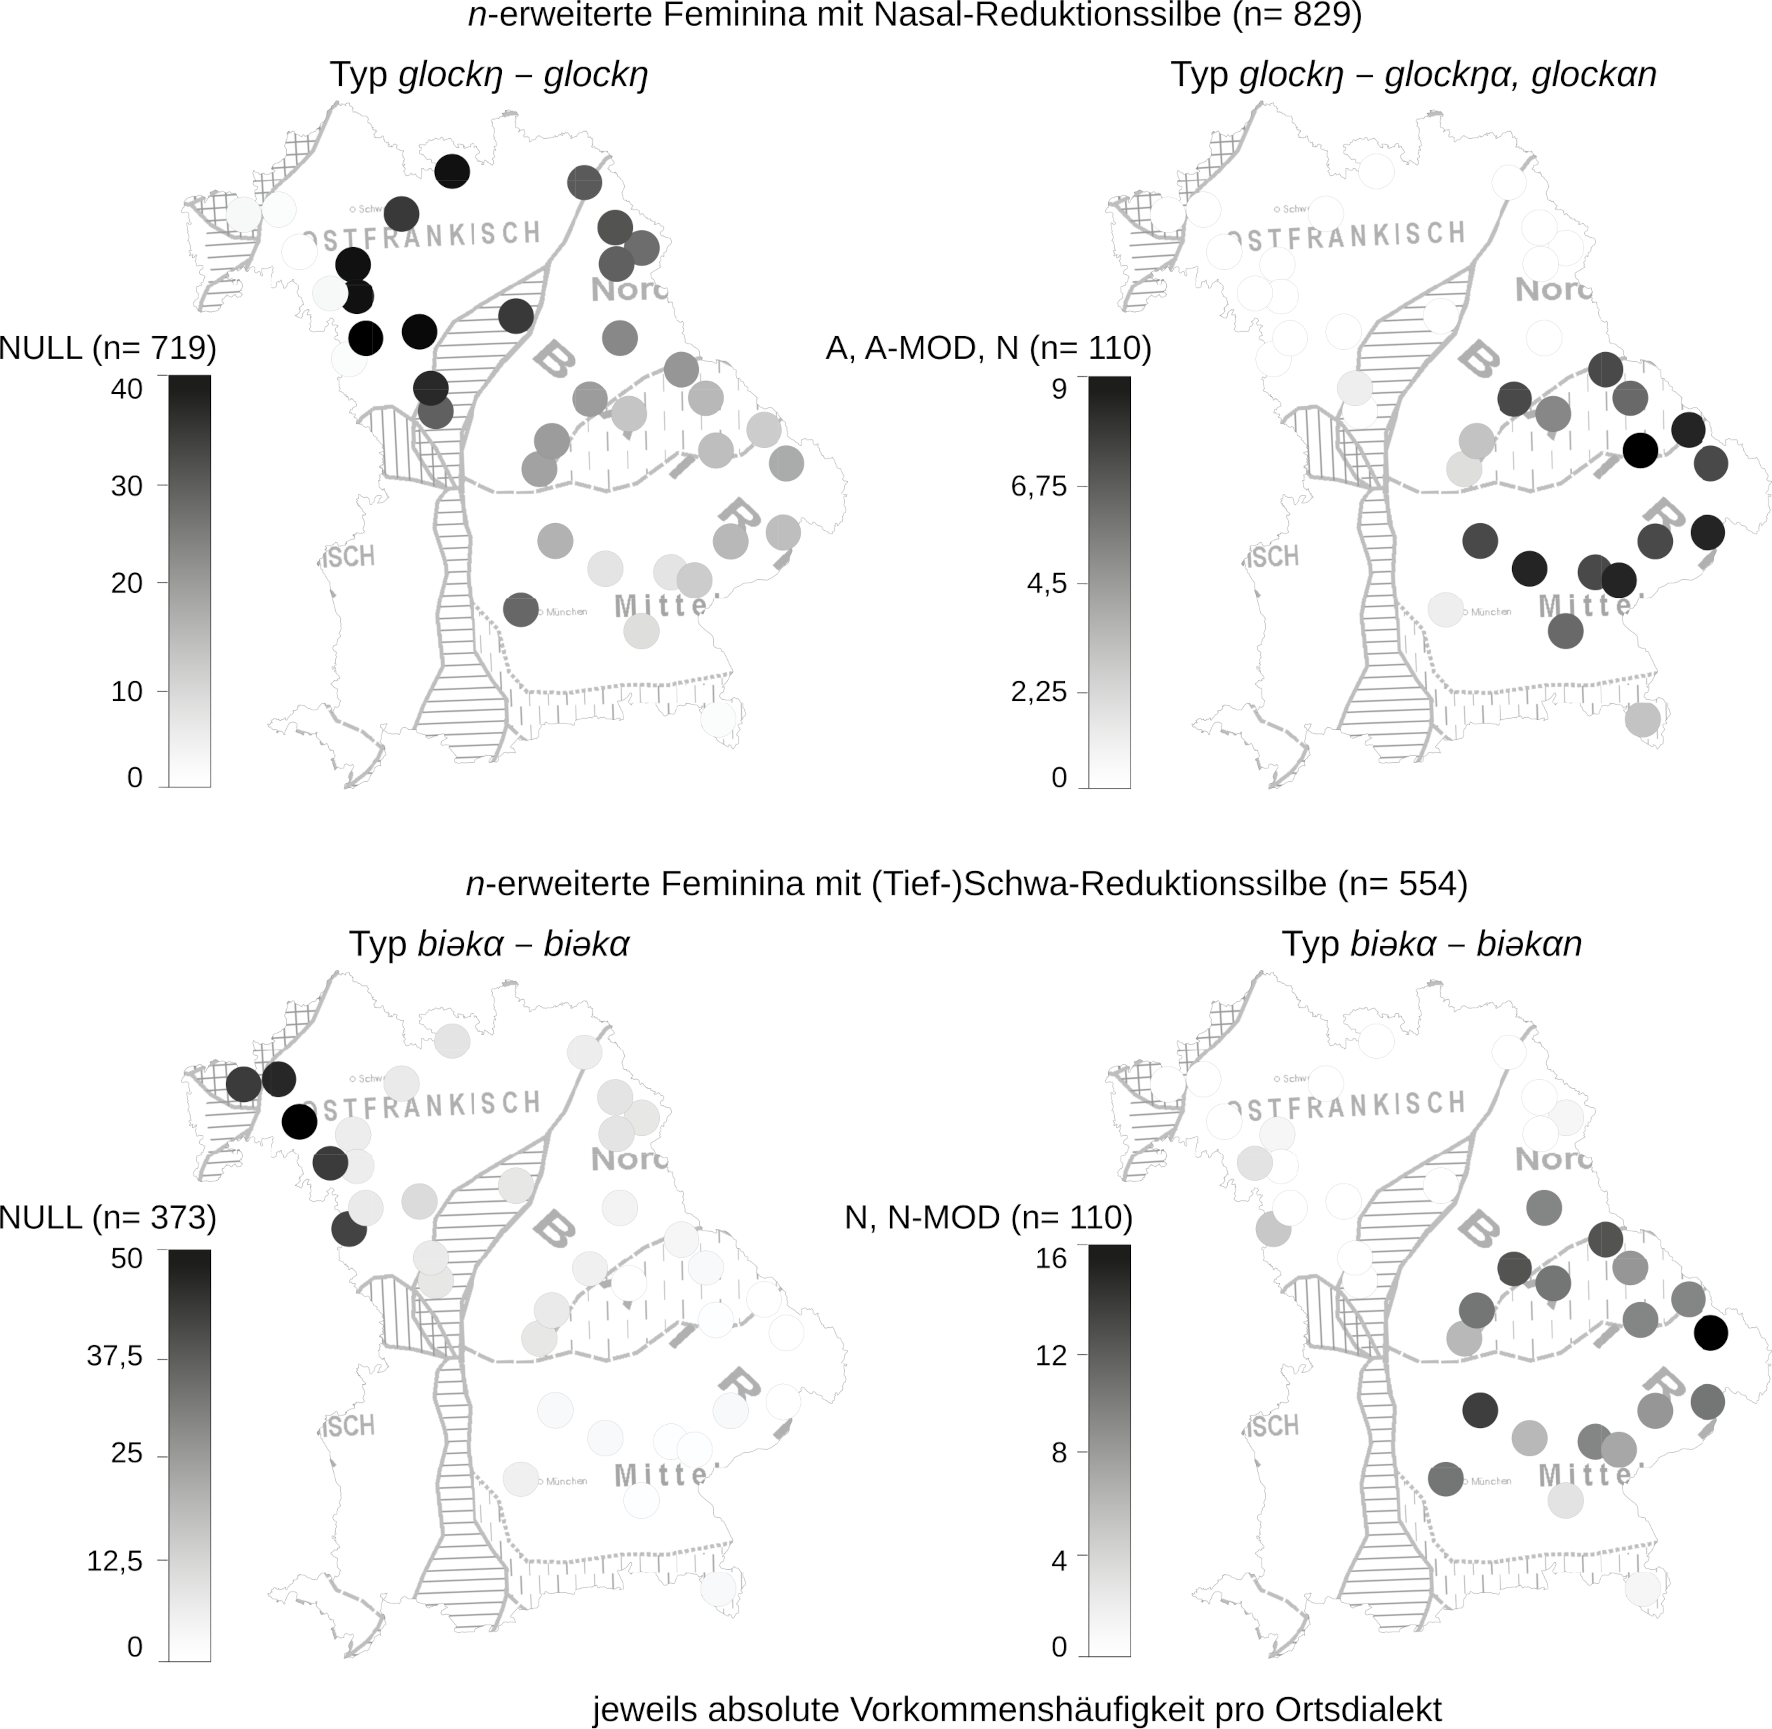
\includegraphics[width=\textwidth]{figures/Karte29.png}
\caption{Areale Häufigkeitsverteilung der Deklinationsklassen NULL, A, N bei \textit{n}{}-erweiterten Feminina ($n=1.383$)}
\label{map:29}
\end{map}


Die Distribution von Tiefschwa- und Nasalsuffix ist im Bair. phonotaktisch durch die Form des Nasalsuffixes im Nom.Sg. konditioniert. Daneben bildet Tief\-schwa-""Re\-duk\-tions\-sil\-be eine produktive Inputbedingung für Nasalsuffigierung und die Abfolge aus Nasal+Tiefschwa-Suffix eine produktive Outputstruktur in diesem Dialektraum (siehe \sectref{sec:8.3.3}). In den Flexionssystemen, in denen Tiefschwa-Suffix ein produktiver Pluralmarker der Feminina (neben den Neutra) ist und zumindest teilweise eine Formalisierung der Konditionierungsprinzipien der Pluralallomorphie erfolgte, ist die Genusopposition zwischen Neutrum und Nicht-Neutrum in der Folge geschwächt.

\subsection{Semantik}\label{sec:8.3.2}
\begin{sloppypar}
Semantische Konditionierung ist von der in \sectref{sec:8.3.3} behandelten formalen Konditionierung zu unterscheiden, da sich semantische Konditionierungsprinzipien auf Merkmale der Inhaltsseite des sprachlichen Zeichens beziehen, während formale Konditionierung die Ähnlichkeit von Merkmalen der Ausdrucksseite betrifft. Eine semantische Steuerung von Deklinationsklassen ist da zu beobachten, wo sich Substantive mit gleichen semantischen Merkmalen auch in der Flexion gleich verhalten. Semantische Distinktionen, die bereits das Deklinationsklassensystem der historischen Vorstufen des Deutschen konditionierten (etwa das besondere flexivische Verhalten von Verwandtschaftsbezeichnungen der historischen \textit{r}{}-Klasse), sind auch in den rezenten Dialekten zu finden. Daneben stellen semantische Distinktionen auch diachron einen Konditionierungsfaktor dar, der einerseits die Reorganisation einzelner Deklinationsklassen und anderseits die Distribution von Allomorphen steuert (vgl. \sectref{sec:3.1.2} sowie den Überblick in \citealt[100--104 und 116--122]{Kürschner2008a}).
\end{sloppypar}

Dass die Abgrenzung genuin semantischer Konditionierung methodisch nicht unproblematisch ist, zeigen \citet{VerslootAdamczyk2018} in ihrer Studie zur irregulären Flexion in den nordseegermanischen Varietäten, indem sie die Brücke zwischen semantischer Steuerung, Analogiebildungen und Kognition schlagen. Die Assoziation von ähnlichen semantischen Merkmalen führt zu Deklinationsklassenwechseln, wenn etwa der historische \textit{i}{}-Stamm \textit{Fisch} (engl. \textit{fish} -- \textit{fish}) analogisch den Nullplural des historischen \textit{a}{}-Neutrums \textit{Schaf} (engl. \textit{sheep} -- \textit{sheep}) annimmt (vgl. \citealt[49--50]{VerslootAdamczyk2018}). Beide Lexeme gehören zu einer semantischen Klasse von Substantiven, die Tiere denotieren und (neben Personen- und Körperteilbezeichnungen) eine hohe absolute und relative Häufigkeit irregulärer Pluralformen aufweisen. Infolge der Korrelation spezifischer semantischer Merkmale und irregulärer Pluralmuster entsteht kognitiv eine „activation relation“ (\citealt[50]{VerslootAdamczyk2018}) zwischen semantischer Kategorie und Pluraltyp: Immer dann, wenn eine spezifische irreguläre Pluralform produziert wird, wird die semantische Kategorie im Gehirn koaktiviert. Bemerkenswert ist hier, dass die Assoziation ähnlicher semantischer Merkmale die eigentlich durch die Vorkommenshäufigkeit bedingte Überrepräsentation irregulärer Pluralformen überdeckt: „For the synchronic (statistical) language learner, the diachronic causal relations are irrelevant; it is rather the model [Regressionsmodell, GN] which includes semantics as an independent variable that represents the learner’s reality“ (\citealt[50]{VerslootAdamczyk2018}). Methodisch besteht daher eine Schwierigkeit darin, die steuernde Wirkung von semantischen Distinktionen von Frequenzeffekten abzugrenzen, da Semantik und hohe Frequenz einander bedingen können (\citealt[26]{VerslootAdamczyk2018}).

Als steuernde Faktoren wurden in dialektologisch-grammatischen Darstellungen die folgenden semantischen Distinktionen identifiziert:

\begin{itemize}\sloppy
\item Nach einem Zahlwort weisen vor allem \textit{Maß-} \textit{und} \textit{Mengenangaben} keine Pluralmarkierung auf, z.\,B. ofr. \teuthoo{drai}{drai} \teuthoo{maus}{maus} \teuthoo{bøiEr}{bøiər} ‚drei Maß Bier‘ oder \teuthoo{tse2.a.}{tsēͅaͅ} \teuthoo{fas}{fas} \teuthoo{wa.i.}{waͅiͅ} ‚zehn Fass Wein‘ (\citealt[§279]{Gebhardt1907}). Nach \citet[105]{Rowley1997} erscheint die unflektierte Singularform nach Zahlwörtern auch bei jenen Substantiven, die in anderen morphosyntaktischen Kontexten eine „besondere Pluralbildung“ haben: ofr. \teuthoo{o.n}{oͅn} \teuthoo{di}{di} \teuthoo{viEdsic}{viədsiX} \teuthoo{haus}{haus} ‚an die vierzig Haus‘.\footnote{Hierzu zählen u.\,a. die Zeiteinheiten \textit{Jahr} und \textit{Tag}, „mancherorts“ \citep[188]{Rowley1997} auch \textit{Woche} (für eine exhaustive Liste siehe \citealt[188]{Rowley1997}). \citet[78]{Wittmann1943} und \citet[318]{Schiepek1908} führen daneben \textit{Nacht} als Zeiteinheit ohne Pluralmarkierung an (gegenüber dem regulären Umlautplural), z~B. \textit{ál Tōch} ‚alle Tage‘, \textit{ál Nācht} ‚alle Nächte‘ (vs. Pl. \textit{Tāch}/\textit{Tēch} bzw. \textit{Nácht}, \citealt[318]{Schiepek1908}).} \citet[§279]{Gebhardt1907} bietet einen Beleg für diese Form morphosyntaktisch bedingter Varianz aus dem Nürnberger Dialekt: ofr. \teuthoo{nau}{nau} \teuthoo{warn}{warn} \teuthoo{di}{di} \teuthoo{leXEr}{leꭗər} \teuthoo{na4igmåxt}{nạiɡm{\burgeroalpha}xt}: \teuthoo{a.2}{āͅ} \teuthoo{lu2x}{lūx}, \teuthoo{tswa2}{tswā} \teuthoo{lu2x}{lūx}, \teuthoo{drai}{drai} \teuthoo{lu2x}{lūx}, \teuthoo{føiEr}{føiər} \teuthoo{lu2x}{lūx} ‚Jetzt werden die Löcher hineingemacht: ein Loch, zwei Loch, drei Loch, vier Loch‘.
\item Das semantische Merkmal \textit{Vorkommen} \textit{in} \textit{Menge} oder \textit{in} \textit{Scharen} und auch das Vorkommen als \textit{Paar} konditioniert im südlichen Nordbair. Nullplural (\citealt[102]{Denz1977}, \citealt[§140.6]{Kollmer1987}, \citealt[148, 159]{Rowley1997}).
\item Im nördlichen Randstreifen des Ofr. sind verschiedene Ausprägungen einer Konditionierung der Deklinationsklasse durch die Distinktionen [${\pm}$\textit{be\-lebt}] und [${\pm}$\textit{menschlich}] belegt (\citealt{HarnischRowley1990}, \citealt[191]{Rowley1997}). Daneben steuert das Belebtheitsmerkmal Klassenwechsel in die schwache Deklination (vgl. \citealt[§20--21]{Micko-Repp1933}).
\item In Teilen des Nordbair. weist eine kleine, semantisch konditionierte Deklinationsklasse „\textit{enge} \textit{Verwandtschaft}“ mit zweisilbiger Singularstammform auf Tiefschwa-Reduktionssilbe ein spezifisches Flexionsparadigma auf (\citealt[137]{Rowley1997}, \citealt[122]{Steininger1994}).
\end{itemize}

In den folgenden Kapiteln werden die Hyperonyme dieser semantischen Distinktionen, Kollektivität (\sectref{sec:8.3.2.1}) und Belebtheit (\sectref{sec:8.3.2.2}), fokussiert. Der As\-pekt der Maß- und Mengenangaben muss dabei ausgeklammert werden, da hierfür systematische Erhebungsdaten fehlen. Dass das Phänomen einer unflektierten Pluralform bei kollektiver Semantik auch im Mittelbair. zu finden ist, zeigt ein Beleg aus Kirchensur: Neben dem Kollektivum \teuthoo{sa4<o<}{sậô} -- \teuthoo{sa4<o<}{sậô} ‚Sau‘ referiert der Umlautplural \teuthoo{sa4<e<}{sậê} auf zählbare Entitäten. Semantische Distinktionen, wie sie etwa die Gewährsperson im mittelbair. Kirchensur vorgenommen hat, und generelle Tendenzen der semantischen Konditionierung konnten nur da systematisch untersucht werden, wo sie Teil des BSA-Fragebuchs waren.

\subsubsection{Kollektivität}
\label{sec:8.3.2.1}
Denotate, die in Mengen vorkommen, weisen im südlichen Nordbair. und im nord\-bair.-""mit\-tel\-bair. Übergangsgebiet Nullplural auf, d.\,h. hier konditioniert eine semantische Distinktion zwischen Kollektivität und Individuiertheit systematisch die Deklinationsklassenzugehörigkeit. Vor dem Hintergrund der untersuchten Daten und aus sprachsystematischer Sicht stellt sich die Frage: Gibt es eine Wahrnehmungsgrenze für Kollektivität? Ein zweiter Forschungsaspekt ergibt sich aus der Formenbildung, da drei flexionsmorphologische Strukturen zu unterscheiden sind: Nullplural, vor allem nach apokopiertem Singularstamm (Typ \teuthoo{erwEs}{erwəs} -- \teuthoo{erwEs}{erwəs} ‚Erbse‘), synkretische Feminina mit \textit{n}{}-Erweiterung in der Nominativ-Singular-Form (Typ \teuthoo{mugN}{muɡŋ} -- \teuthoo{mugN}{muɡŋ} ‚Mücke‘), sowie Synkretismen durch sogenannte Markiertheitsumkehrungen (Typ \teuthoo{ebvl}{ebvl} -- \teuthoo{ebvl}{ebvl} ‚Äpfel‘, vgl. \citealt[54]{Roth1940}). Synkretismen dieses Typs sind insofern das Ergebnis von Markiertheitsumkehrungen im Sinne \citegen[48--58]{Mayerthaler1981}, als die Pluralform die frequentere und damit unmarkierte Form darstellte; nach \citet[835]{Tiersma1982} liegt „local markedness“ vor: „When the referent of a noun naturally occurs in pairs or groups, and/or when it is generelly referred to collectively, such a noun is locally unmarked in the plural.“ Synkretismen infolge von Markiertheitsumkehrung (bzw. „local markedness“) kommen mit variierender arealer Geltung in allen untersuchten Dialekten vor (\mapref{map:23}).

Anhand der Form \teuthoo{dsi."bv5}{dsīͅbv̩} (neben \teuthoo{dse\$2bv}{dsē̤bv}) -- \teuthoo{di}{di} \teuthoo{la.NE}{laͅŋə} \teuthoo{dse4bv}{dsẹbv} ‚Zopf‘ (ofr.-hess. Wiesthal) konnte in \sectref{sec:7.1.3.2} gezeigt werden, dass die Markiertheitsumkehrung historisch vor jenen phonologischen Prozessen erfolgt ist, die die Stammvokalquantität und -qualität affizierten (hier die Hebung von mhd. \textit{ö} in Dehnung). Markiertheitsumkehrungen in den rezenten Dialekten können damit als lexikalisierte Formen analysiert werden; die höhere Gebrauchsfrequenz der Pluralform und die Generalisierung des Pluralmarkers sind konserviert. Die Lexikalisierung dieser Formen (respektive die Reanalyse als Singularform) erklärt auch die sekundäre, distinkte Pluralmarkierung, die vereinzelt belegt und nicht das Ergebnis morphophonologischer Alternation ist, etwa \teuthoo{s\#dôe{\textasciitilde}îl}{šd{\aufstrih}e{\aufstrih}l} -- \teuthoo{s\#dôe{\textasciitilde}îln@}{šd{\aufstrih}e{\aufstrih}ln̥} ‚Stuhl‘ (nordbair.-mittelbair. Blaibach).

Auch jene innerparadigmatischen Ausgleichsformen, die zu einer Generalisierung des Nasalsuffixes bei Feminina und einigen Maskulina und Neutra geführt haben, können im Zusammenhang mit Markiertheitsumkehrungen gesehen werden: „Von Fall zu Fall ließe sich sicher so argumentieren“ \citep[159]{Rowley1997}. Dies gilt insbesondere bei der semantischen Gruppe paarig vorkommender Körperteile, die in den untersuchten Dialekten mit \textit{n}{}-Erweiterung belegt sind: \teuthoo{oAn}{oαn} -- \teuthoo{oAn}{oαn} ‚Ohr‘ und \teuthoo{auN}{auŋ} -- \teuthoo{auN}{auŋ} ‚Auge‘ im südlichen Nordbair. und Mittelbair., \teuthoo{bagN}{baɡŋ} -- \teuthoo{bagN}{baɡŋ} ‚Backe‘ im Ofr. (daneben vereinzelt \textit{Hachse}, \textit{Knie}, \textit{Wade}, vgl. \sectref{sec:7.1.3.1}). Insgesamt bleibt \citet[189]{Rowley1997} jedoch „skeptisch, ob der Vorgang adäquat als ‚Markiertheitsumkehrung‘ aufgefaßt werden kann, da mir der Begriff zu uneingeschränkt, dessen deskriptiver Wert zu beliebig erscheint“ (siehe hierzu auch \citealt[144]{Bybee2010}).

Alternativ zum Konzept der Markiertheitsumkehrung, das stärker Frequenzeffekte als eine semantische Steuerung von Allomorphie spiegelt, ist bei den synkretischen Singular- und Pluralformen von Feminina mit \textit{n}{}-Erweiterung tatsächlich eher semantische Konditionierung anzunehmen. Im südlichen Nordbair. steht -- anders als in den ofr. Dialekten -- eine numerusdistinkte additive Markierung als Mittel der Formenbildung zur Verfügung (Typ \teuthoo{das\#n}{dašn} -- \teuthoo{das\#nA}{dašnα} und \teuthoo{biEkA}{biəkα} -- \teuthoo{biEkAn}{biəkαn}), die bei einigen dieser \textit{n}{}-erweiterten Feminina aber unterbleibt. \citet[§140.6]{Kollmer1987} differenziert für diese Klasse von Feminina verschiedene semantische Gruppen mit kollektiver Bedeutung: paarig vorkommende Körperteile (z.\,B. \textit{nian} ‚Niere‘), in Scharen oder Mengen vorkommende Lebewesen (u.\,a. \textit{Ente}, \textit{Taube}, \textit{Fliege}, \textit{Mücke}), Früchte (u.\,a. \textit{Birne}, \textit{Zwetschge}) und andere Dinge, die in Mengen von Bedeutung sind, insbesondere Abfall (etwa \teuthoo{s\#a2itn}{šāitn} ‚Holzspäne‘, \teuthoo{s\#iakN}{šiakŋ} ‚Kopfschuppen‘, \teuthoo{da.ksn}{daͅksn} ‚Nadelholzzweige‘).

In den Dialekten des südlichen Nordbair. und  nordbair.-mittelbair. Übergangsgebiets kann das Nebeneinander von numerusdistinkten und -syn"-kre"-ti"-schen Pluralformen der \textit{n}{}-erweiterten Feminina genauso wie der Nullplural bei apokopiertem Singularstamm durch die semantische Distinktion von Kollektivität (vs. Individuiertheit) erklärt werden (vgl. \citealt[190]{Rowley1997}). In den mittelbair. Dialekten weisen fem. Denotate, die in Mengen oder in Scharen vorkommen (Kleinstlebewesen, Früchte), dagegen eher numerusdistinkte Formen auf (meist mit apokopierter Singularstammform und Nasalsuffix in der Pluralform). Für das südliche Nordbair. und das Übergangsgebiet kann für die Distribution der Allomorphe (Nullmarkierung vs. eine Form additiver Markierung) bei den rezenten Entsprechungen der historischen \textit{n}{}- und \textit{ô}{}-Deklination damit semantische Distinktion mit arealer (d.\,h. dialektraumspezifischer) Geltung angenommen werden. Offenbleiben muss jedoch, wo in diesem Dialektgebiet die Grenze für eine kollektive Lesart verläuft. So weisen die Kleinstlebewesen \textit{Mücke}, \textit{Fliege} und \textit{Bremse} Synkretismen auf, nicht aber \textit{Wespe} (Typ \teuthoo{weS}{weʃ} -- \teuthoo{weSn}{weʃn}). Bei den in Mengen vorkommenden Früchten \textit{Birne} und \textit{Zwetschge} sind nur synkretische Formen belegt, vereinzelt bei \textit{Kirsche} aber nicht (z.\,B. \teuthoo{k,\_e).Es\#5}{k͓ʰe\klammeruntenpost{}ͅəš̩} -- \teuthoo{k,\_e).Es\#5n@}{k͓ʰe\klammeruntenpost{}ͅəš̩n̥} im nordbair.-mittelbair. Bernhardswald). Möglich scheint eine Wahrnehmungsgrenze von Kollektivität, wobei noch zu zeigen ist, inwiefern es hier interdialektale Unterschiede gibt. Der typologische Vergleich zeigt indes, dass eine binäre Unterscheidung von Kollektivität vs. Individuiertheit eine Vereinfachung eines eher skalaren Phänomens ist (vgl. \citealt[82]{Corbett2000}).

\subsubsection{Belebtheit}
\label{sec:8.3.2.2}
Eine Restrukturierung der historischen mask. \textit{n}{}-Deklination erfolgte im Spätmittelhochdeutschen und Frühneuhochdeutschen entlang einer Skala von Belebtheitsmerkmalen (vgl. \sectref{sec:3.1.2}). Eine Konditionierung der Allomorphie durch die semantische Distinktion [${\pm}$belebt] und das Hyponym [+menschlich] ist auch in den dialektalen Flexionssystemen unterschiedlich prägend (vgl. \citealt{Kürschner2008b}). Im sprachtypologischen Vergleich stellt Belebtheit als semantisches Merkmal eine universale konzeptuelle Kategorie dar, die in verschiedenen Sprachen von struktureller Relevanz ist, was Belebtheit wiederum zu einem besonders salienten Merkmal macht (\citealt[181]{Comrie1981}, siehe auch \citealt{Köpcke2000a}). Belebtheit ist dabei nach \citet[178]{Comrie1981} hierarchisch konzeptualisiert: menschlich > belebt > unbelebt. Einzelsprachlich kann Belebtheit feiner abgestuft konzeptualisiert oder auch mit weiteren Merkmalen (etwa Definitheit oder Genus) korreliert sein. \citet[56]{Corbett2000} beispielsweise setzt in seiner Belebtheitshierarchie als weitere Stufe Verwandtschaftsbezeichnungen an, Ausgangspunkt dieser Hierarchie ist die Sprecherperspektive (Sprecher > Adressat > 3.Ps. > verwandt > menschlich > belebt > unbelebt). \citet{Kasper2017} fasst diese Form eines Kontinuums von semantischen Distinktionen terminologisch daher passend als „Belebtheits- oder Empathiehierarchie“ (vgl. \citealt{Kasper2020}).

Typologische Arbeiten wie die von \citet{Comrie1981} und \citet{Corbett2000} zeigen, dass Belebtheit und die Realisierung flexivischer Kategorien wie Numerus und Kasus einzelsprachlich korreliert sein können. So sind distinkte Singular- und Pluralformen und damit eine eindeutige Markierung der Numerusinformation charakteristisch für Denotate und Nominalphrasen mit hohem Belebtheitsgrad (vgl. \citealt[180]{Comrie1981}, \citealt[56]{Corbett2000}). \citet[181--182]{Comrie1981} setzt das Belebtheitsmerkmal mit einer weiteren semantischen Distinktion in Zusammenhang: Individuation vs. Kollektivität. Belebte Denotate werden eher als Individuen (und damit als zählbar) wahrgenommen als unbelebte Denotate. Die Belebtheitshierarchie kann nach \citet[192]{Comrie1981} auf eine Hierarchie der Individuation oder vielmehr auf eine Salienz-Hierarchie reduziert werden. Salienz bezieht sich dabei auf „the way in which certain actants present in a situation are seized on by humans as foci of attention, only subsequently attention being paid to less salient, less individuate objects“ \citep[192]{Comrie1981}. Eine solches Kontinuum, das die Merkmale Individuiertheit und Belebtheit gleichermaßen integriert, schlägt \citet[180]{Sasse2015} vor: Eigennamen > Menschen > Tiere > Unbelebte Konkreta > Abstrakta ${\geq}$ Kollektiva (siehe auch \citealt[659]{Sasse1993}). Dass es plausibel ist, für die semantischen Distinktionen [${\pm}$belebt] und [${\pm}$kollektiv] „a complex intertwining rather than [\ldots] a single, linear hierarchy“ \citep[192]{Comrie1981} anzunehmen, zeigen die Synkretismen bei der semantischen Gruppe von in Scharen vorkommenden Kleinstlebewesen im südlichen Nordbair. (\sectref{sec:8.3.2.1}). Dass \textit{Mücke}, \textit{Fliege} und \textit{Bremse} Synkretismen aufweisen, nicht aber \textit{Wespe} spricht dafür, dass es innerhalb dieser semantischen Gruppe mit dem Merkmal [+belebt] eine Abstufung der Kollektivitätswahrnehmung gibt. \citet{Kasper2020} zeigt zudem, dass auch das semantische Merkmal der Belebtheit hierarchisch zu verstehen ist und u.\,U. einer weiteren Differenzierung bedarf: Ein unlängst geschlachtetes, totes Tier kann auf der Belebtheits- und Empathiehierarchie (und gleichermaßen in der Sprecherkognition) zwischen [+belebt] und [$-$belebt] verortet werden, solange die körperliche Integriert des Tieres gewahrt, es also noch nicht zerlegt ist. Um semantische Distinktionen wie diese deskriptiv erfassen zu können, braucht es Dialektdaten mit einer höheren Granularität, als sie in den BSA-Daten zu finden ist; die folgenden Analysen konzentrieren sich daher auf die semantischen Distinktionen [${\pm}$belebt], [${\pm}$menschlich], [${\pm}$verwandt].

In \sectref{sec:8.2.1} wurde gezeigt, dass für die historisch schwachen Maskulina der \textit{n}{}-Deklination in den rezenten Dialekten (1) Variation dahingehend zu beobachten ist, ob die obliquen Kasus im Singular mit oder ohne Nasalsuffix realisiert werden (Typ \teuthoo{An}{αn} \teuthoo{ho2sn}{hōsn} vs. \teuthoo{An}{αn} \teuthoo{ho.s}{hoͅs}), und (2) diachron eine semantisch konditionierte Reorganisation der Deklinationsklasse stattgefunden hat: Bei Maskulina mit meist unbelebtem Denotat wird das Nasalsuffix in den Nom.Sg. übertragen (Typ \teuthoo{s\#tekN}{štekŋ} -- \teuthoo{s\#tekN}{štekŋ} ‚Stecken‘) und es erfolgt ein Wechsel in die Nullklasse oder in ein distinktes Pluralmarkierungsverfahren (vgl. \mapref{map:27}). Dass es in den Dialekten unterschiedliche Ausprägungen von Belebtheitskonditionierung bei der schwachen Deklination gibt und dass sogar eine areale Staffelung vorliegen kann, zeigt \citet[191]{Rowley1997} für den nördlichen Rand des Ofr. (siehe auch \citealt{HarnischRowley1990} sowie \sectref{sec:7.2.2}). Im ofr. Waldau (Thüringen) ist der mhd. Stand der \textit{n}{}-Deklination vor der semantisch konditionierten Restrukturierung erhalten, d.\,h. es liegt keine semantische Konditionierung der \textit{n}{}-Deklination vor (vgl. \sectref{sec:3.1.2}). Im weiteren ofr. Randstreifen, etwa im Ludwigstädter und Kronacher Raum, ist dagegen eine Differenzierung von Maskulina mit der Distinktion [−belebt] mit Nasal im Nom.Sg. (Typ \textit{Balken} -- \textit{Balken}) und [+belebt] mit schwacher Deklination erfolgt. Im Coburger Raum ist die schwache Flexion im Singular auch bei belebten Denotaten abgebaut (im Plural erscheint Nasalsuffix). In der Übergangszone zwischen Coburger und Kronacher Raum ist die schwache Flexion im Singular nur bei belebten Denotaten abgebaut; bei menschlichen Denotaten ist sie hingegen erhalten.

\vfill
\begin{map}[H]
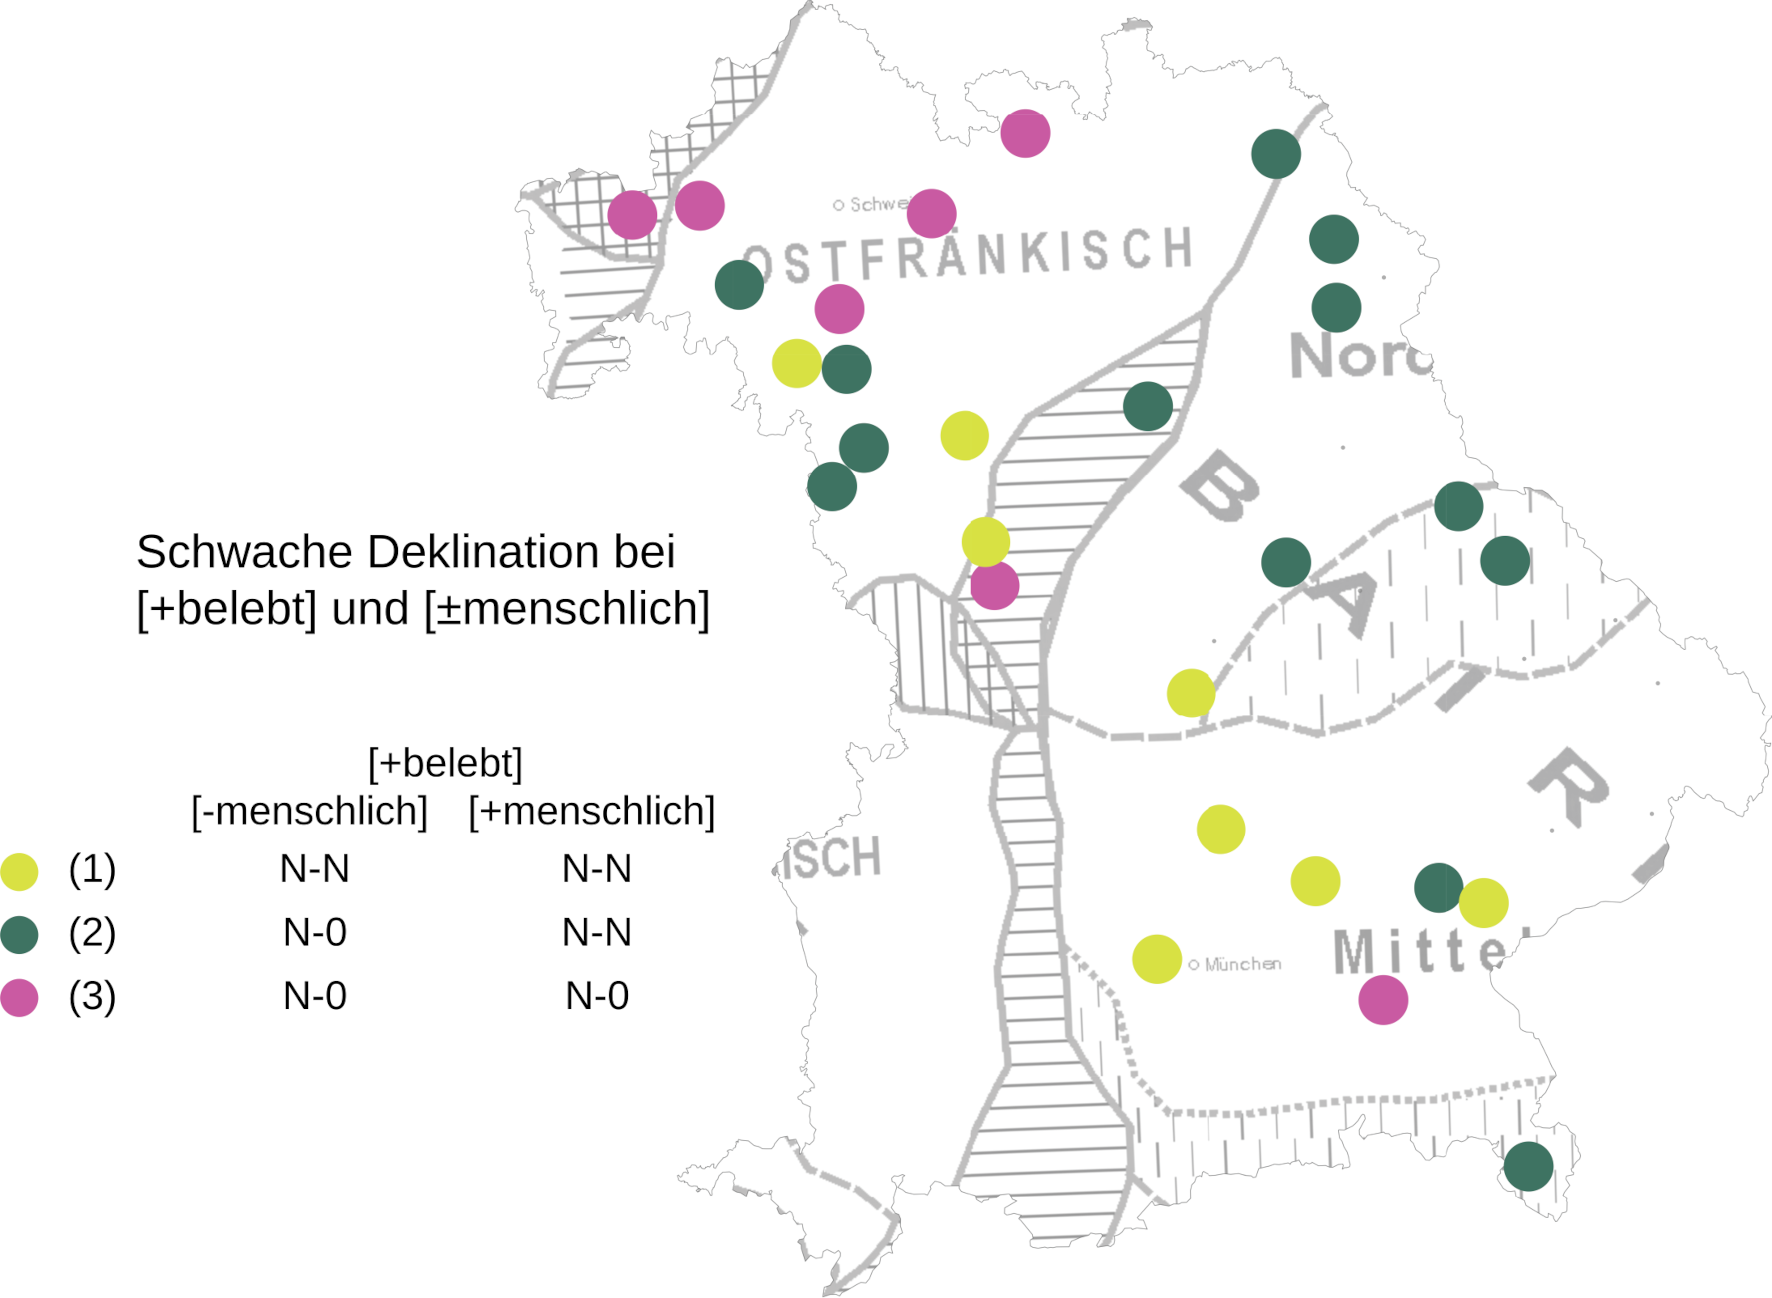
\includegraphics[width=\textwidth]{figures/Karte30.png}
\caption{Semantische Konditionierung der „schwachen“ Teilklassen N-N und N-0 durch die Distinktionen [+belebt] und [${\pm}$menschlich] bei den rezenten schwachen Maskulina ($n=124$)\protect\footnote{In den BSA-Daten ist nur ein schwaches Maskulinum mit dem Merkmal [+menschlich] in den obliquen Singularkasus erhoben worden (\textit{Bauer}); die Maskulina mit dem Merkmal [+belebt] und [$-$menschlich] sind \textit{Hase}, \textit{Hecht}, \textit{Karpfen}, \textit{Ochse}, \textit{Rabe} (\textit{Krack}), \textit{Ratte} und \textit{Spatz} (\textit{Sperk}).} }
\label{map:30}
\end{map}
\vfill\pagebreak

\mapref{map:30} zeigt, dass es auch in den Dialekten des UGs eine areale Distribution von drei Typen der Belebtheitsdistinktion gibt.\footnote{Bedingt durch die dünne Datenlage in den BSA-Teilprojekten des mittelbair. Dialektraums sind die kartierten Typen nur vorsichtig zu interpretieren (Voraussetzung war jeweils min. ein Beleg für die Distinktion [{${\pm}$}menschlich]. Teilweise finden sich keine Akkusativformen für Maskulina mit dem Merkmal [$-$menschlich], weshalb von einer Typisierung und Kartierung abgesehen wurde.}  Bei Typ (1), der vor allem im Nordbair. und im westlichen Ofr. zu finden ist, flektieren sämtliche belebte Maskulina nach dem Muster der schwachen Deklination (Deklinationsklasse N-N). Typ (2) beschreibt die Distinktion [${\pm}$menschlich] und damit eine Differenzierung des Belebtheitsmerkmals: Das Nasalsuffix der obliquen Singularkasus erscheint nur bei Maskulina mit dem Merkmal [+menschlich], Maskulina mit den Merkmalen [+belebt] und [$-$menschlich] weisen im Singular keine Kasusflexion auf (Deklinationsklasse N-0). Zudem ist der vollständige Abbau der Kasusflexion im Singular bei allen belebten Maskulina belegt; dieser Typ (3) ist vor allem im Unterofr. und im von \citet{Rowley1997} beschriebenen Coburger Raum zu finden (Tiefenbohrungspunkt Ahorn).

Dass bei Typ (1) das Merkmal [+belebt] die Deklinationsklassenzugehörigkeit steuert, ist in einem Teil der nordbair. Dialekte zu beobachten. Hier weist das his\-to\-ri\-sche \textit{n}{}-Maskulinum \textit{Karpfen} Nasalsuffix im obliquen Singularkasus auf, es liegt (vor der diachronen Folie) eine Art Doppelsuffigierung aus Nasalsuffix und vokalisch realisierter Reduktionssilbe mhd. -\textit{en} vor: Nom.Sg. \teuthoo{k,\_a.rpfA}{k͓ʰaͅrpfα} -- Akk.Sg. \teuthoo{An}{αn} \teuthoo{k,\_a.rpfAn}{k͓ʰaͅrpfαn} -- Nom.Pl. \teuthoo{k\_arpfAn}{kʰarpfαn} im nordbair. Kallmünz (vgl. Abschnitte~\ref{sec:7.2.1} und \ref{sec:7.2.2}). Das his\-to\-risch schwache, aber unbelebte Maskulinum \textit{Stecken} hingegen hat synkretische Formen im Singular: Nom.Sg. \teuthoo{s\#de.kA}{šdeͅkα} -- Akk.Sg. \teuthoo{s\#de.kA}{šdeͅkα} \teuthoo{s\#de.kA}{šdeͅkα} ‚einen Stecken (in den Boden) stecken‘ -- Nom.Pl. \teuthoo{s\#de.kAn}{šdeͅkαn} (Kallmünz). Im Nordbair. scheint es also tatsächlich das Merkmal [+belebt] zu sein, dass schwache Flexion im Singular und auch Deklinationsklassenwechsel steuert, etwa des historischen \textit{a}{}-Stamms \textit{Hecht}: Nom.Sg. \teuthoo{he4cd}{hẹXd} -- Akk.Sg. \teuthoo{An}{αn} \teuthoo{he4cdn@}{hẹXdn̥} -- Nom.Pl. \teuthoo{he4cdn@}{hẹXdn̥} im nordbair. Kallmünz (vgl. \citealt[§32.2]{Paul1968}).

\citet{DammelGillmann2014} haben für den „Sonderweg“ der historisch schwachen Maskulina argumentiert, dass die formale Distinktion zwischen Nom.Sg. und den obliquen Singularkasus durch das Belebtheitsmerkmal bedingt ist, da belebte Referenten sowohl als prototypisches Agens als auch als Patiens vorkommen; durch das schwache Flexionsmuster erfolgt eine formale Kodierung der unterschiedlichen syntaktischen Rollen.\footnote{Gleichwohl stellt Belebtheit nur einen Faktor dar, der aber nicht isoliert betrachtet werden dürfe, sondern im Zusammenhang mit dem gesamten Deklinationsklassensystem und dem morposyntaktischen Kontext der Nominalphrase (\citealt[212]{DammelGillmann2014}).} Belebtheitseffekte führen (vor dem Hintergrund des Relevanzprinzips) also zu einer „Relevanzerhöhung für Kasus“ (\citealt[211]{DammelGillmann2014}, ausführlicher \sectref{sec:5.2}). Gleichzeitig ist eine rezente Tendenz zum Abbau der schwachen Flexion im Singular zu beobachten (Gen./""Dat./""Akk.""Sg. \textit{Menschen} > \textit{Mensch} -- \textit{Menschen}). \citet[212]{DammelGillmann2014} folgern daraus, dass auch Belebtheit langfristig nicht vor dem Abbau des Kasusausdrucks am Substantiv schützt. Nach \citet{Köpcke2000a, Köpcke2002} ist allerdings nicht nur das Belebtheitsmerkmal zentral für das Schema der schwachen Maskulina, sondern erst die Kombination aus dem Merkmal [+menschlich] und dem phonologisch-prosodischen Merkmal finales Schwa (etwa in \textit{Bube}) ist ein verlässlicher Hinweis auf die schwache Deklination (siehe \sectref{sec:5.3.2}). Finales Schwa bei den Maskulina ist nach \citet[119]{Köpcke2000a} ein „Agentivitätsmarker“: Nur die schwache, nicht aber die starke Deklination weist ihn auf; Deflexion vollzieht sich ausgehend von der Peripherie (\textit{dem Mensch}), schließt aber nicht den prototypischen Kern des Schemas (mit finalem Schwa) ein \citep[105]{Köpcke2002}.

Zumindest für die nordbair. Dialekte muss für das Schema der schwachen Maskulina angenommen werden, dass phonologische Merkmale weniger zentral sind: Auch ein zweisilbiges Maskulinum wie \textit{Karpfen} weist schwache Flexion auf. Hier ist der zentrale Konditionierungsfaktor das semantische Merkmal [${\pm}$belebt]. Da finales Schwa als „formales Korrelat“ (\citealt[119]{Köpcke2000a}) des semantischen Merkmals [+menschlich] in den oobd. Dialekten apokopiert ist, scheint die Semantik neben Genus der einzige (verbleibende) Hinweisgeber auf die schwache Deklination zu sein -- zumindest in jenen Dialekten, die eine distinkte Kasusform im Singularparadigma erhalten haben.

Grundsätzlich wären hier weitere, systematisch erhobene Daten wünschenswert. Denn auch in den Dialekten mit Belebtheitskonditionierung des Typs (1) und (2) weisen nicht alle belebten Maskulina Nasalsuffigierung in den obliquen Singularkasus auf; vor allem \textit{Spatz} und daneben auch \textit{Ratte} und -- als Einzelbeleg im ofr. Gebsattel -- \textit{Ochse} flektieren nach dem Muster N-0 (siehe hierzu auch \sectref{sec:7.2.2}). Hier braucht es weitere Daten, um eine mögliche Abstufung des semantischen Merkmals Belebtheit abbilden oder den Abbau der Kasusmarkierung auf mögliche Frequenzeffekte zurückführen zu können.

In den untersuchten Dialekten finden sich weitere Fälle von Deklinationsklassenwechsel in das Pluralverfahren mit Nasalsuffix: bei dem historischen \textit{i}{}-Stamm \textit{Fuchs} im südlichen Nordbair. und im Mittelbair., \textit{Hecht} im Nordbair. und Ofr. sowie im Ofr. bei den \textit{a}{}-Stämmen \textit{Hund}, \textit{Knecht} und dem \textit{i-}Stamm \textit{Wirt}.\footnote{\citet[§20--21]{Micko-Repp1933} führt daneben noch den Wechsel der historisch starken Maskulina \textit{Wolf}, \textit{Bär}, \textit{Eber}, \textit{Hengst} und \textit{Krebs} in die schwache Flexion an.} Bei den Maskulina ist die Pluralmarkierung durch Nasalsuffix dialektübergreifend mit dem semantischen Merkmal [+belebt] assoziiert.\footnote{Ob diese Lexeme auch in die schwache Kasusflexion im Singular gewechselt sind, lässt sich nur für \textit{Hecht} sagen, da die übrigen Maskulina nicht in den obliquen Kasus erhoben wurden: \textit{Hecht} flektiert nur im Nordbair. (inkl. Übergangsgebiet) nach dem Muster der schwachen Deklination (Klasse N-N), in den übrigen (ofr.) Dialekt erfolgte Wechsel in die Deklinationsklasse N-0.} Gleichzeitig bewahren andere Maskulina mit belebtem oder menschlichem Denotat die historische Deklinationsklasse, etwa die \textit{i}{}-Stämme \textit{Fisch} und \textit{Frosch}.

Bei den Feminina ist \textit{n}{}-Plural bei der großen Gruppe der historischen \textit{n}{}- und \textit{ô}{}-Deklination und nicht exklusiv bei belebtem Denotat zu finden. Allerdings findet eine semantische Konditionierung von Nullplural vs. Nasalsuffix bei Feminina mit dem Merkmal [+belebt] entlang der Individuierungshierarchie statt: Belebte Denotate, die individuell und nicht als in Mengen oder Scharen vorkommend wahrgenommen werden, haben eine distinkte Pluralform mit Nasalsuffix, etwa der historische n-Stamm \textit{Katze} (Typ \teuthoo{katS}{katʃ} -- \teuthoo{katSn}{katʃn}) oder die Klassenwechsler \textit{Geiß} (Typ \teuthoo{ga2s}{ɡās} -- \teuthoo{ga2sn}{ɡāsn}) und \textit{Magd} (Typ \teuthoo{ma2d}{mād} -- \teuthoo{ma2dn}{mādn}) im Ofr.

Im südlichen Nordbair. und in Teilen des Mittelbair. konditioniert das semantische Merkmal [+verwandt] in Kombination mit der prosodisch-phonotaktischen Inputbedingung einer Tiefschwa-Reduktionssilbe schwache Flexion im Singular: bei den Feminina mit einer distinkten Dativ-Singular-Form (Typ Nom./Akk.Sg. \teuthoo{mutA}{mutα} -- Dat.Sg. \teuthoo{mutAn}{mutαn} -- Pl. \teuthoo{mutAn}{mutαn}), bei den maskulinen Verwandtschaftsbezeichnungen mit Nasalsuffix in den obliquen Singularkasus (Akk./Dat.Sg. \teuthoo{våtAn}{v{\burgeroalpha}tαn}, vgl. Abschnitte~\ref{sec:7.2.2} und \ref{sec:8.3.3.1}). Verwandtschaftsbezeichnungen sind auf \citegen{Corbett2000} Belebtheitshierarchie noch näher am Sprecher angeordnet, weshalb die semantische Konditionierung dieses spezifischen Flexionsmusters durch die -- in \citegen{Comrie1981} Terminologie -- höhere Salienz erklärt werden kann.

\subsection{Formale Konditionierung}\label{sec:8.3.3}
\begin{sloppypar}
Die in \sectref{sec:3.2} vorgestellten Studien zu Konditionierungswandel haben ergeben, dass diachron ein Abbau von Komplexität der Konditionierung von Deklinationsklassen erfolgt, da zu dem primären Konditionierungsprinzip Genus formale Konditionierungsfaktoren und die in \sectref{sec:8.3.2} behandelte semantische Konditionierung hinzukommen (vgl. \citealt{DammelKürschner2008}, \citealt{Kürschner2008a}). Diese Formalisierung der Konditionierung ist auch in den untersuchten Dialekten zu beobachten. Es sind vor allem prosodische und phonotaktische Steuerungsprinzipien, die diachron zu einer Reorganisation der Klassen führen und auch synchron die Distribution der Pluralallomorphe in einzelnen Dialekten steuern. Die zu beobachtenden prosodischen und phonotaktischen Konditionierungsprinzipien sind spezifisch für Teile der untersuchten bair. Dialekte. Die formale Konditionierung bedingt hier additive Pluralmarkierung (gegenüber Null in Dialekten ohne diese Kodierung) oder steuert die Distribution der additiven Allomorphe.
\end{sloppypar}

Formale Konditionierung ist, wie \citet[33]{Harnisch1987} herausstreicht, auch kog"-ni"-tiv vorteilhaft, da phonologische Muster es „erlauben, lernpsychologisch (mnemotechnisch) gesehen, Voraussagen über das Wie der morphologischen Kodierung“ zu treffen. Damit ist für einige bair. Dialekte eine Zweiteilung der Formenbildung zu beobachten: eine Formalisierung der Konditionierung der additiven Markierung einerseits und anderseits ein hohes Maß an Lexikalisierung morphophonologischer Alternationen, die zwar mnemotechnisch aufwändiger sind, dafür aber einen direkten Zugriff auf die gesamte Form erlauben (vgl. \citealt[59]{Harnisch1990} und \sectref{sec:5.1}).

\subsubsection{Prosodische Konditionierung}
\label{sec:8.3.3.1}
Die dialektraumspezifische Distribution von additiven und Nullpluralen in den ofr. und bair. Dialekten des UGs ist das Ergebnis wiederum dialektraumspezifischer prosodischer Input- und Outputkonditionierung, d.\,h. Konditionierung, die entweder die Form und strukturelle Eigenschaften der Basisform oder des Flexionsprodukts betrifft. Im südlichen Nordbair. und in Teilen des Mittelbair. sind genusübergreifend Formen von prosodischer Inputkonditionierung bei zweisilbigen Singularstämmen auf Reduktionssilbe zu finden, die den Plural regelmäßig additiv markieren; im Ofr. und im nördlichen Nordbair. hingegen erscheint Nullplural. Genusspezifisch ist dabei allerdings die Spezifikation der Inputbedingung, da neben der prosodischen Struktur die Form der Reduktionssilbe bei den Genera unterschiedlich steuernd wirkt. 

Regelmäßig bei allen Genera erfolgt die additive Markierung mit Nasalsuffix bei \textit{el}-Reduktionssilbe (realisiert als [l̥] oder vokalisiert zu [i] oder [e] im Mittelbair.). \mapref{map:31} zeigt, dass additive Pluralmarkierung durch Nasalsuffix bei Feminina in weiten Teilen des UGs verbreitet ist (ausgenommen sind das nördliche Nordbair. und der westliche Vokalisierungsstreifen des Ofr.). Bei Maskulina und Neutra hingegen ist diese Form der Markierung vor allem im südlichen Nordbair. und vereinzelt im Mittelbair. belegt. Bei den Neutra handelt es sich ausschließlich um Diminutiva (siehe \sectref{sec:8.3.4} zur diatopisch variierenden Pluralmarkierung der Diminutiva).\footnote{Die Schwankung der absoluten Zahlen von Nasalsuffigierungen nach \textit{el}{}-Reduktionssilbe bei Neutra ergibt sich vor allem auch aus Zusammensetzung der Daten. Im mittelbair.-südbair. Ramsau etwa sind auch da Diminutivformen belegt, wo im BSA-Fragebuch Simplizia erhoben wurden. In den übrigen Ortsdialekten sind hingegen nur dann Diminutiva in den Daten zu finden, wenn diese systematisch abgefragt wurden.} In den ofr. Dialekten, die Nasalsuffix-Plural bei Feminina auf -\textit{el} haben, weisen die Maskulina Nullplural auf. Daneben ist in einem Teil des ofr.-nordbair. Raums Nasalsuffigierung bei \textit{el}{}-Reduktionssilbe laut \citet[169]{Rowley1997} sogar „grundsätzlich ausgeschlossen“, d.\,h. auch bei den Feminina \textit{Wurzel}, \textit{Gabel} usw. (siehe auch \citealt[148]{Rowley1997}).



\begin{map}
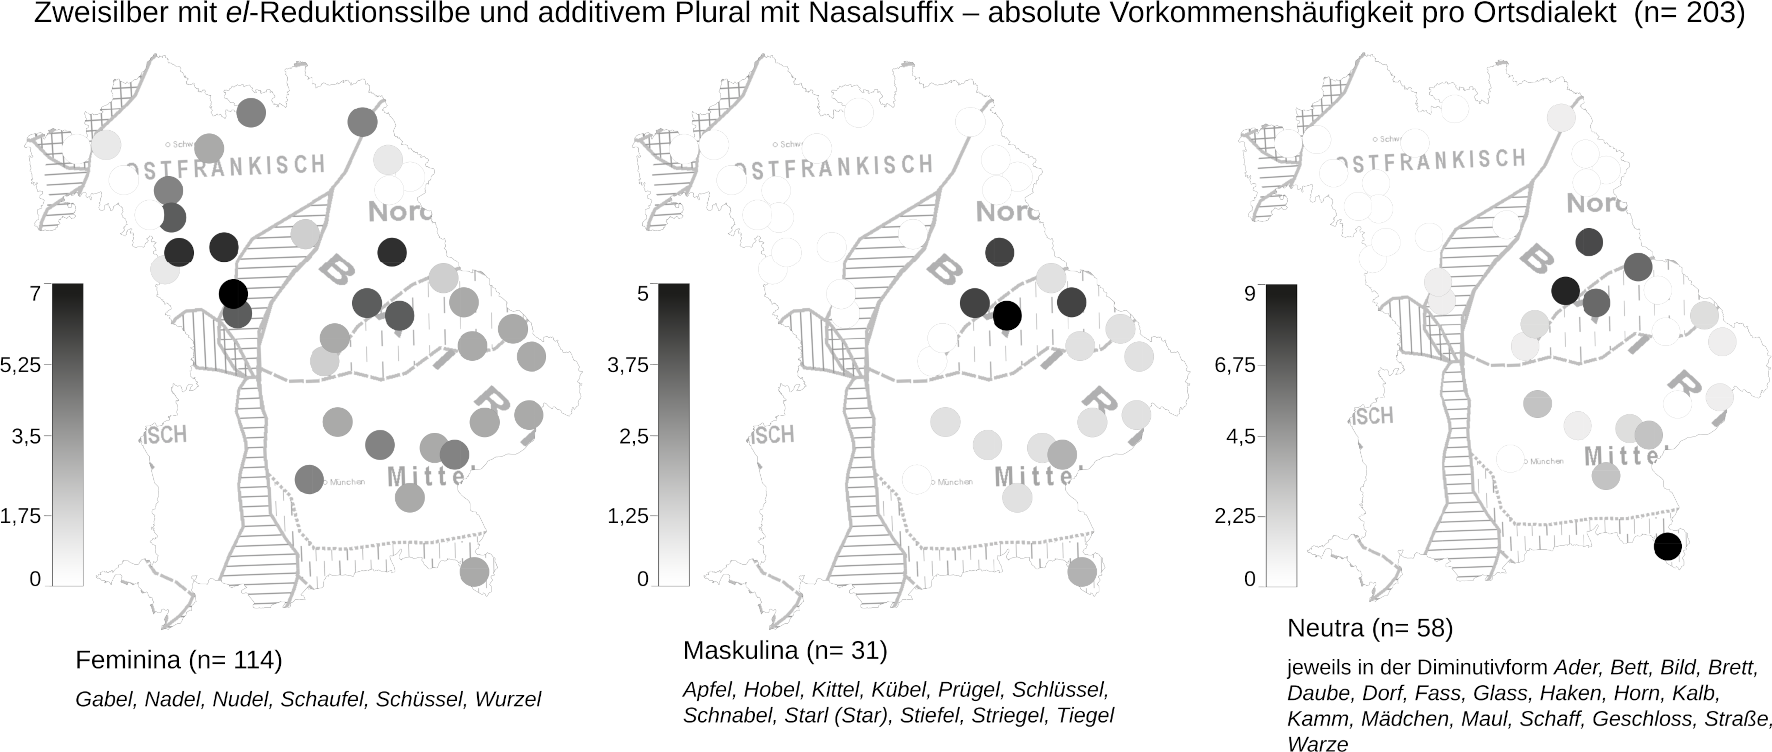
\includegraphics[width=\textwidth]{figures/Karte31.png}
\caption{Prosodische Inputkonditionierung bei \textit{el}{}-Reduktionssilbe}
\label{map:31}
\end{map}

Diversen dialektologisch-grammatischen Darstellungen zufolge erscheint die \textit{n}{}-Suffigierung bei Maskulina nur dann, wenn kein Umlaut-Plural vorliegt (vgl. \citealt[158]{Rowley1997}, \citealt[421]{Schirmunski1962}, \citealt[§801]{Schmeller1821}, \citealt[§11e]{Weitzenböck1942}). Im südlichen Nordbair. (Tiefenbohrungspunkt Bernhardswald) finden sich indes Belege historischer \textit{i}{}-Maskulina mit \textit{el}{}-Reduktionssilbe, die auch Umlautplural aufweisen (Pl. \teuthoo{ds\#na\$wl°@n@}{dšna̤wl̥̑n̥} ‚Schnäbel‘, \teuthoo{epfl°@n@}{epf‌l̥̑n̥} ‚Äpfel‘, siehe \sectref{sec:8.2.1}). Hier hat die prosodische Input-Konditionierung zu kumulativer Markierung geführt. \citet[153]{Rowley1997} zufolge sind die additiven Pluralformen mit Nasalsuffix bei den Maskulina fakultative Markierungen, die bei fehlender Disambiguierung der Numerusinformation im syntaktischen Kontext erfolgt (vgl. \citealt[158]{Rowley1997} sowie \sectref{sec:9.2}). Auch \citet[421]{Schirmunski1962} nennt Beispiele für ein Fehlen des \textit{n}{}-Suffixes bei vorausgehendem Zahlwort: \teuthoo{s\#lisln}{šlisln} ‚Schlüssel‘, aber \teuthoo{tswaI2\textsuperscript{n}}{tswaı̄\textsuperscript{n}} \teuthoo{s\#lisl}{šlisl} ‚zwei Schlüssel‘.\footnote{Dies können die eigenen Daten weder bestätigen noch widerlegen, da es sich um isolierte Abfrage-Items handelt und keine Aussagen über semantisch-pragmatische Kontextbedingungen von distinkten oder synkretischen Formen gemacht werden können.}



\begin{map}
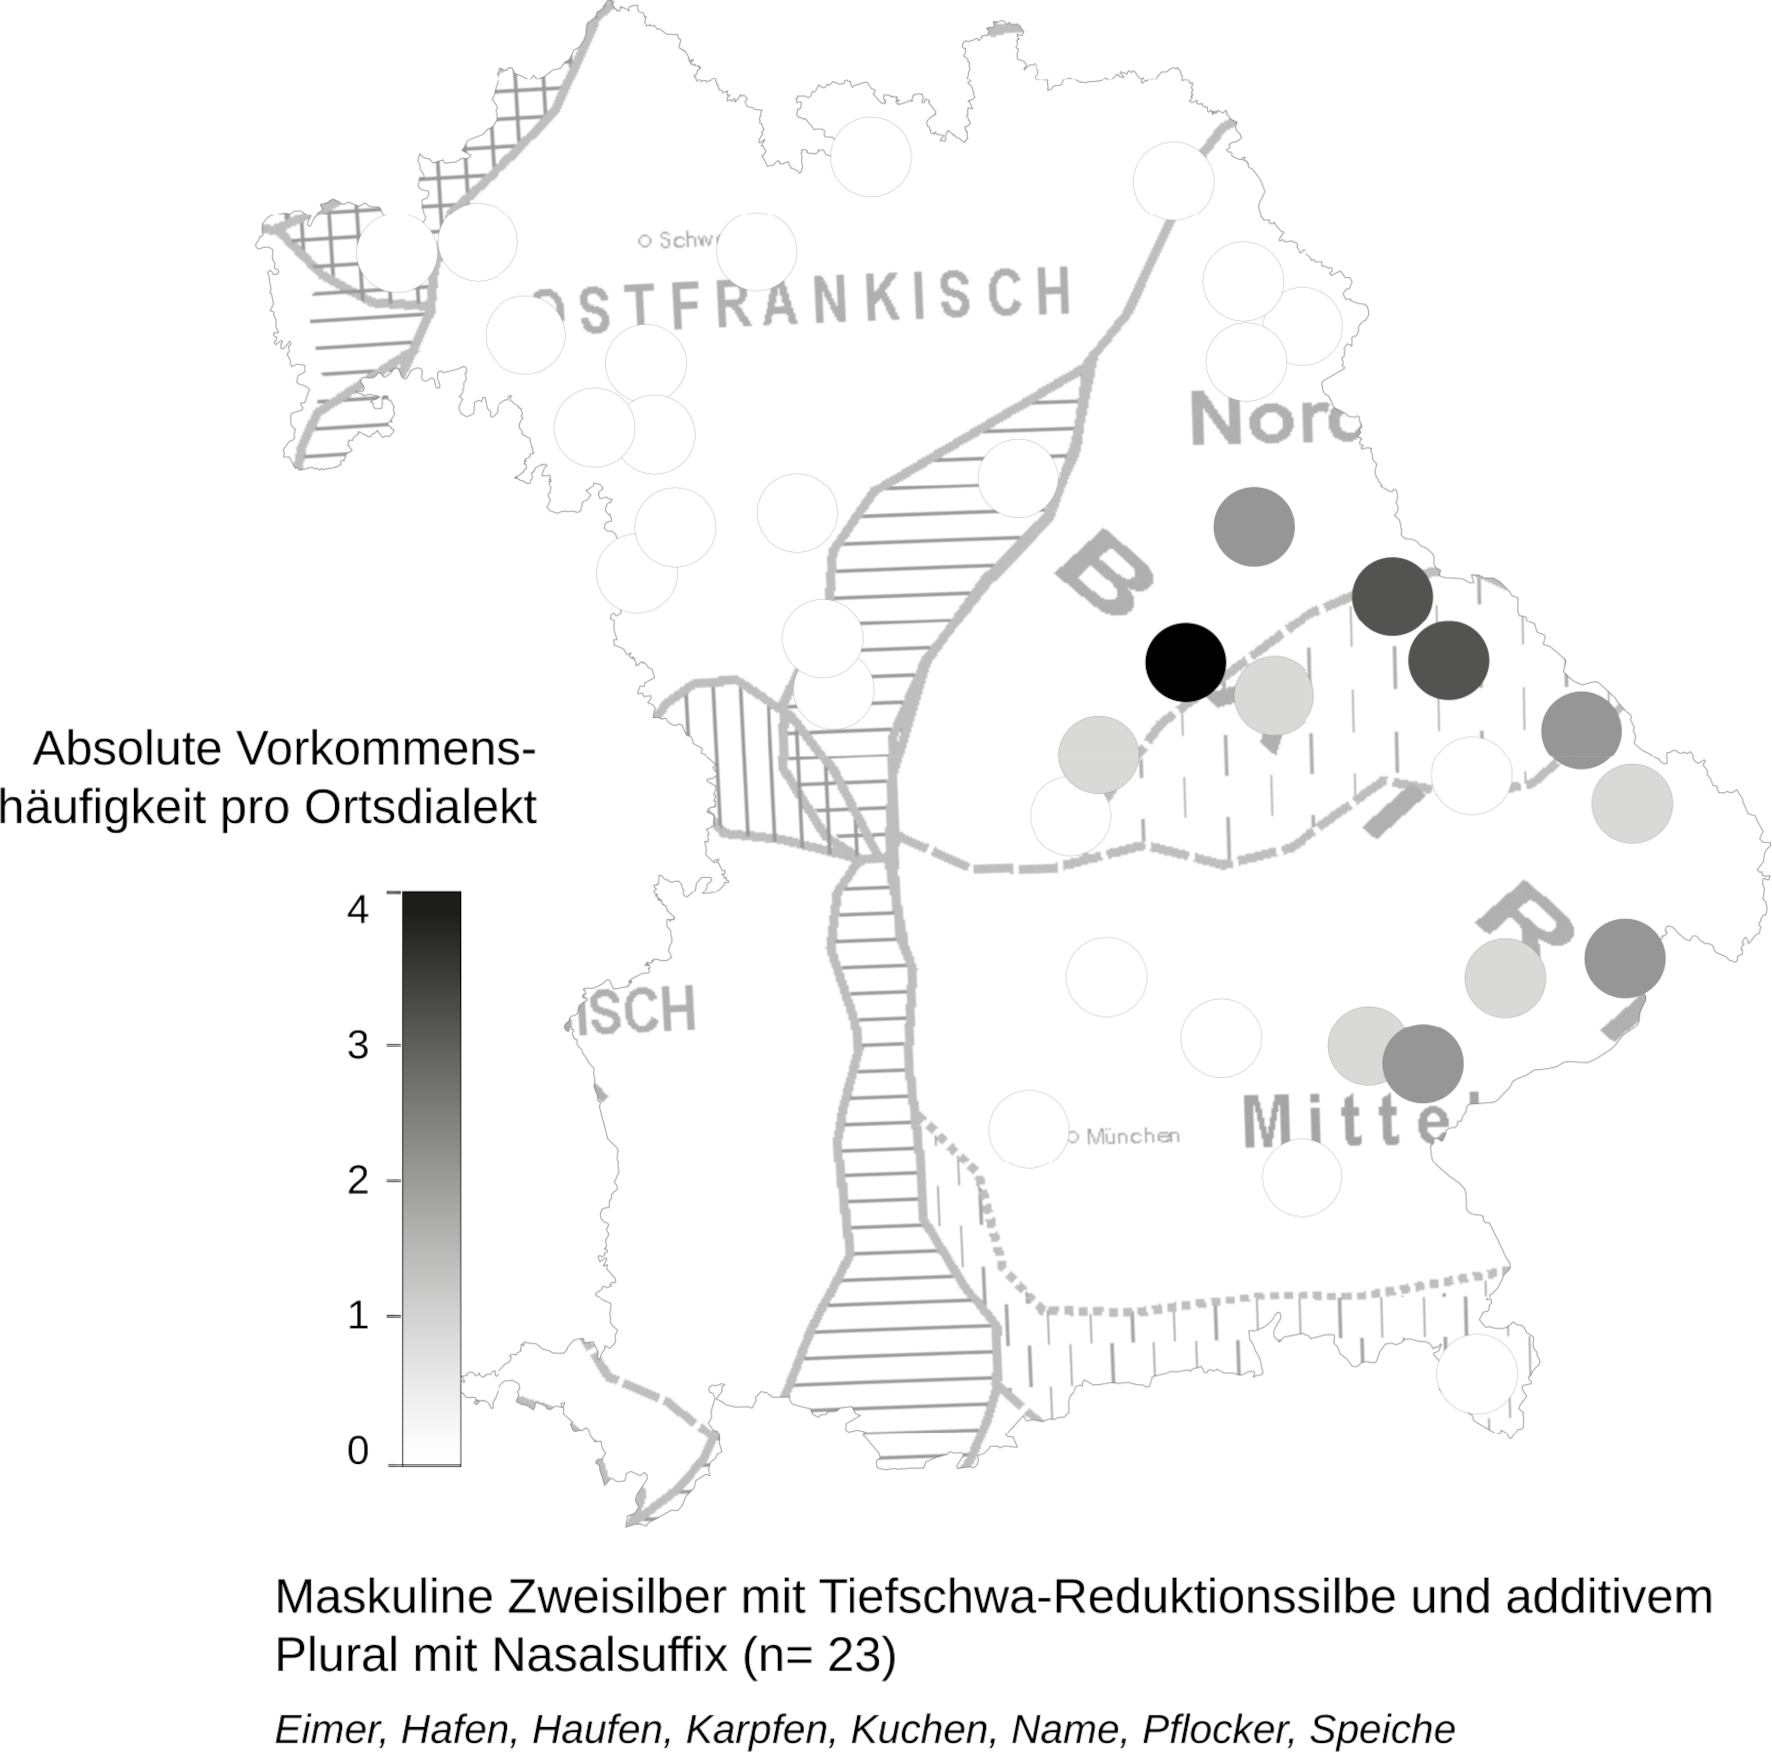
\includegraphics[width=\textwidth]{figures/Karte32.png}
  \caption{Prosodische Inputkonditionierung bei zweisilbigen Maskulina mit Tiefschwa-Reduktionssilbe}
  \label{map:32}
\end{map}

Eine weitere Form der Inputkonditionierung besteht aus Zweisilbigkeit und Tiefschwa-Reduktionssilbe für Feminina und Maskulina. Methodisch stellt sich auch hier die Frage, ob Tiefschwa als heteromorphische Variante für mhd. \mbox{-\textit{er}} und -\textit{en} klassifiziert wird oder einen eigenen Typus darstellt (siehe die Diskussion in \sectref{sec:7.1.1.1} sowie \citealt[128, 166--168]{Rowley1997}). Unter Berücksichtigung der arealen Distribution der Pluralformen und der diachronen Folie ist es bei den Feminina von Vorteil, zunächst die Differenzierung von mhd. -\textit{er} und -\textit{en} auch für die rezenten Dialekte beizubehalten, da sie aufzeigt, inwiefern die Inputkonditionierung einer Tiefschwa-Reduktionssilbe tatsächlich dialektraumspezifisch ist. Pluralformen mit Nasalsuffix (Typ \teuthoo{biEkA}{biəkα} -- \teuthoo{biEkAn}{biəkαn} ‚Birke‘), bei denen Tiefschwa die phonotaktisch bedingte Entsprechung der Reduktionssilbe mhd. -\textit{en} im Nom.Sg. ist, finden sich im südlichen Nordbair. und im Mittelbair. (\mapref{map:4} und \mapref{map:29}). Die Markierung mit Nasalsuffix bei Reduktionssilbe mhd. \mbox{-\textit{er}} (Typ \teuthoo{kha.mA}{khaͅmα} -- \teuthoo{kha.mAn}{khaͅmαn} ‚Kammer‘) ist indes in allen Dialekten des UGs belegt und entspricht der historischen Deklination (fem. \textit{ô}, ebenso bei \textit{Ader} und \textit{Feder}). Für das Bair. ist damit bei den Feminina eine Inputkonditionierung aus Zweisilbigkeit und Tiefschwa-Reduktionssilbe anzunehmen; hier werden mhd. \mbox{-\textit{er}} und -\textit{en} in der Realisierung als -\textit{α} in den rezenten Flexionssystemen nicht differenziert. Auch die semantisch konditionierte Deklinationsklasse „enge Verwandtschaftsbezeichnungen“, die \citet[137]{Rowley1997} für Teile des Nordbair. anführt und die im Paradigma Nasalsuffigierung aufweist, ist nicht nur durch das semantische Merkmal, sondern auch durch die prosodische Inputkonditionierung einer Tiefschwa-Reduktionssilbe bedingt (vgl. \citealt[170]{Rowley1997}, siehe Abschnitte~\ref{sec:7.2.2} und \ref{sec:8.3.2.2}).


Bei den Maskulina erfolgt im südlichen Nordbair. und im Mittelbair. die additive Pluralmarkierung regelmäßig bei vokalisch realisiertem Nasalsuffix (Typ \teuthoo{hoafA}{hoafα} -- \teuthoo{hoafAn}{hoafαn} ‚Haufen‘) und vereinzelt auch bei \textit{er}{}-Reduktionssilbe, etwa bei \teuthoo{e<.mA}{êͅmα} -- \teuthoo{e<.mAn}{êͅmαn} ‚Eimer‘ (nordbair.-mittelbair. Blaibach) oder bei \teuthoo{gho2da}{ɡhōda} -- \teuthoo{gho2dan}{ɡhōdan} ‚Kater‘, \teuthoo{ghe2va}{ɡhēva} -- \teuthoo{ghe2van}{ɡhēvan} ‚Käfer‘ (\citealt[128 und 154]{Rowley1997}, vgl. \citealt[§38]{Kollmer1985}). Hier liegt -- der phonetischen Form des Singularstammes entsprechend -- ebenfalls eine konditionierende Inputbedingung zweisilbiger Singularstamm mit Tiefschwa-Reduktionssilbe vor. Laut \citet[153]{Rowley1997} ist die additive Markierung mit Nasalsuffix bei den Maskulina auf Tiefschwa-Reduktionssilbe (wie auch bei Maskulina auf -\textit{el}) fakultativ, \citet[421]{Schirmunski1962} beschreibt sie als „weniger konsequent“ als bei \textit{el}{}-Reduktionssilbe.


Doch auch wenn die additive Markierung bei den Maskulina kein sehr frequentes Phänomen ist (vgl. \mapref{map:32}), so lassen die Belege doch den Schluss zu, dass Nasalsuffigierung (und damit ein Deklinationsklassenwechsel) dann realisiert wird, wenn keine andere Form der Numerusdistinktion vorliegt. Der historische \textit{i}{}-Stamm \textit{Hafen} etwa wird im Bair. mit Umlautplural markiert (neben zahlreichen Markiertheitsumkehrungen); nur im mittelbair. Grafenau liegt keine Vokalalternation vor, es erscheint Nasalsuffigierung (\teuthoo{ho.<v5A}{hôͅv̩α} -- \teuthoo{ho.<vAn}{hôͅvαn}). Dass die beschriebene Inputbedingung in diesem Teil des Bair. einen produktiven prosodischen Steuerungsfaktor darstellt, zeigen zudem vereinzelte Belege, die nicht auf alte Reduktionssilben zurückgehen. Bei Komposita mit dem Zweitglied \textit{{}-tag} wird im UG teilweise die Nebenakzentsilbe reduziert (z.\,B. ofr. \textit{doog} > \mbox{-\textit{ic}}, \citealt[338]{Schmidt1905}).\footnote{Vgl. \citet[22--23]{Köhler1934}, \citet[Karte 12]{Roth1940}, \citet[15]{Schießl1909}.} Infolge der Reduktion erscheint im bair. Teil des UGs für das Kompositum \textit{Werktag} die prosodische Struktur eines Zweisilbers auf Tiefschwa-Reduktionssilbe. Im nordbair.-mittelbair. Übergangsgebiet sind der Inputkonditionierung entsprechend additive Pluralformen mit Nasalsuffix belegt: \teuthoo{we.2AdA}{wēͅαdα} -- \teuthoo{we.2AdAn}{wēͅαdαn} (Zwiesel) und \teuthoo{weEdA}{weədα} -- \teuthoo{weEdAn}{weədαn} (Bern\-hards\-wald, der Simplex \textit{Tag} hat dagegen Null- oder Umlautplural).\footnote{\citet[422]{Schirmunski1962} führt daneben den Beleg \teuthoo{fraI2dA}{fraı̄dα} -- \teuthoo{fraI2dAn}{fraı̄dαn} ‚Freitag‘ an.}


Für jene Feminina, die das Nasalflexiv der obliquen Kasus im Nom.Sg. aufweisen, kann im Bair. eine prosodische und phonotaktische Inputkonditionierung angenommen werden (zur Singularstammbildung siehe Abschnitte~\ref{sec:7.1.3.1} und \ref{sec:8.3.1.3}). Die prosodische Struktur ist auch hier zweisilbig, die Reduktionssilbe mhd. -\textit{en} wird als Nasal (Typ \teuthoo{das\#n}{dašn} ‚Tasche‘) oder vokalisch (Typ \teuthoo{biEkA}{biəkα} ‚Birke‘) in Abhängigkeit vom Stammauslaut realisiert. Die Form des Suffixes, das bei der additiven Markierung dieser zweisilbigen Feminina mit \textit{en}-Reduktionssilbe erscheint, ist phonotaktisch konditioniert: Nach Nasal erscheint \textit{α}{}-Suffix (Typ \teuthoo{das\#n}{dašn} -- \teuthoo{das\#nA}{dašnα}), nach Tiefschwa Nasalsuffix (Typ \teuthoo{biEkA}{biəkα} -- \teuthoo{biEkAn}{biəkαn}, vgl. \sectref{sec:8.3.3.2}). \figref{fig:15} illustriert, dass eben diese Inputstruktur auf Tief\-schwa-Re\-duk\-tions\-sil\-be das Muster für die mask. Deklinationsklassenwechsel bildet. Mit Blick auf die Interdependenz der Konditionierungsprinzipien ist bemerkenswert, dass in Nabburg im mittleren Nordbair. die additive Markierung nach Tiefschwa-, nicht aber nach Nasalsuffix im Nom.Sg. belegt ist (vgl. \mapref{map:4} und \mapref{map:29}). Die zweisilbige Inputstruktur ist damit eine notwendige, aber keine hinreichende Bedingung; die phonotaktische Inputbedingung (hier die Form der Reduktionssilbe) wirkt gleichermaßen steuernd (additive Markierung erfolgt bei Tief\-schwa-Re\-duk\-tions\-sil\-be, nicht aber nach Nasal).



\begin{figure}
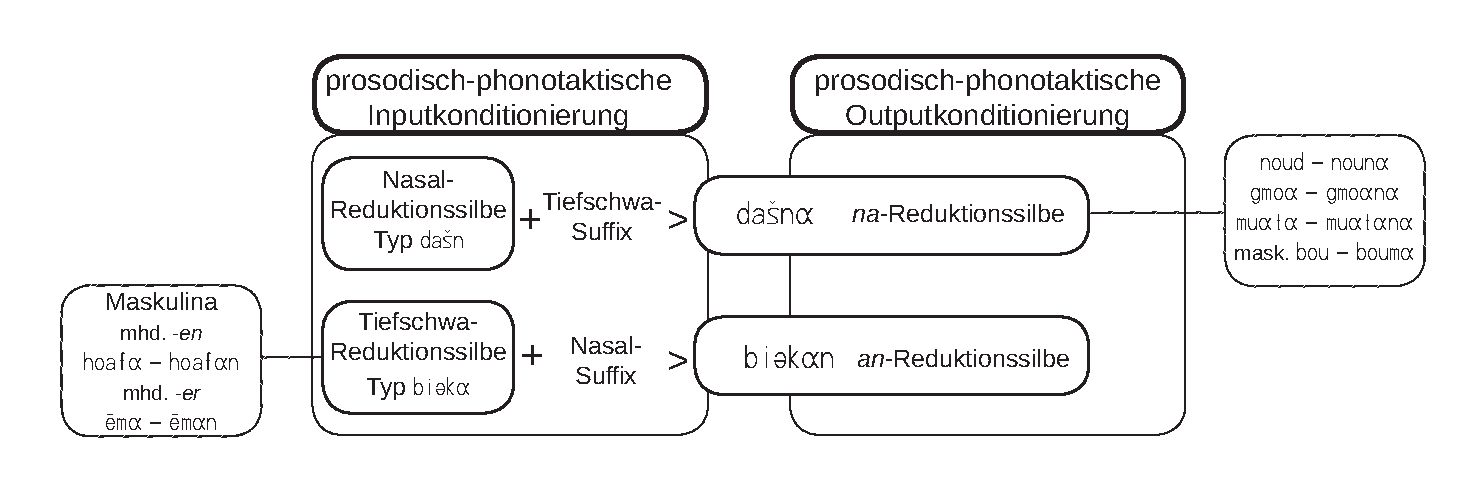
\includegraphics[width=\textwidth]{figures/Outputkonditionierung.pdf}
\caption{Input- und Outputkonditionierung der Feminina}
\label{fig:15}
\end{figure}

Neben diesen Formen der Inputkonditionierung ist in den bair. Dialekten auch eine prosodische Konditionierung auf Basis des Outputs für fem. Pluralformen festzustellen. Es handelt sich um zwei präferierte Outputstrukturen, die in den Dialekten des südlichen Nordbair. und im Mittelbair. parallel vorkommen und in Kombination mit phonotaktischer Konditionierung beschrieben werden müssen. Ein Typus besteht darin, dass Pluralformen präferiert zweisilbig sind und auf Reduktionssilbe {-\textit{αn}} enden, er findet sich bei verschiedenen Singularstammformen und als Ergebnis folgender additiver Verfahren:

\begin{itemize}\sloppy
\item „Doppelsuffigierung“ bei Feminina mit als Tiefschwa realisiertem Nasalsuffix in der Nominativ-Singular-Form (Typ \teuthoo{biEkA}{biəkα} -- \teuthoo{biEkAn}{biəkαn} ‚Birke‘)
\item Suffixalternation \textit{{}-n} > -\textit{αn} bei Feminina mit Nasalsuffix in der Nominativ-Singular-Form (Typ \teuthoo{biEkN}{biəkŋ} -- \teuthoo{biEkAn}{biəkαn})
\item Additive Markierung mit \textit{αn}{}-Suffix von einsilbigen, meist apokopierten Singularstämmen auf Plosiv (Typ \teuthoo{biEk}{biək} -- \teuthoo{biEkAn}{biəkαn}) oder mit vokalischem Auslaut (\teuthoo{vrau}{vrau} -- \teuthoo{vrauAn}{vrauαn} ‚Frau‘, vgl. \citealt[153]{Rowley1997})
\item Additive Markierung mit \textit{n}{}-Suffix von Simplizia mit Tief\-schwa-""Re\-duk\-tions\-sil\-be (Typ \teuthoo{o2dA}{ōdα} -- \teuthoo{o2dAn}{ōdαn} ‚Ader‘)
\end{itemize}

Die zweite präferierte Outputstruktur endet auf Reduktionssilbe {-\textit{nα}}. Dieser Bedingung entsprechen die \textit{n}{}-erweiterte Feminina des Typs \teuthoo{das\#n}{dašn} -- \teuthoo{das\#nA}{dašnα} sowie auf Nasal auslautende Simplizia mit \textit{α}{}-Suffix (Typ \teuthoo{diAn}{diαn} -- \teuthoo{diAnA}{diαnα} ‚Dirn‘). Daneben finden sich Klassenwechsel von Feminina, die his"=to"=risch keinen Plural mit Nasalsuffix bildeten, etwa die historischen \textit{i}{}-Stämme \teuthoo{nôo(+u(+d5}{n{\aufstrih}õ\klammerobenpost{}ũ\klammerobenpost{}d̩} -- \teuthoo{nôo(+u(+nA}{n{\aufstrih}õ\klammerobenpost{}ũ\klammerobenpost{}nα} ‚Naht‘ (nordbair. Oberdolling) oder \teuthoo{d5i“4a}{d̩ị̄a} -- \teuthoo{d5i“4AnA}{d̩ị̄αnα} ‚Tür‘ (mittelbair. Kirchensur) sowie der kontrahierte Stamm \teuthoo{gmo>+A+}{ɡmỗα̃} -- \teuthoo{gmo2A2nA}{ɡmōᾱnα} ‚Gemeinde‘ (mittelbair.-südbair. Ramsau, vgl. 	\tabref{tab:37} und \citealt[160]{Rowley1997}). In diesen Fällen war Deklinationsklassenwechsel in eine Pluralform auf Na"=sal+""Tief"=schwa durch die Outputbedingung gesteuert. Bemerkenswert mit Blick auf die Herausbildung des nhd. Systems, das durch die Outputbedingung eines (idealiter trochäischen) Plurals auf Reduktionssilbe geprägt ist, sind dabei dreisilbige Pluralformen, die auf zwei Reduktionssilben schließen: \teuthoo{bmuAtA}{bmuαtα} -- \teuthoo{muAdAnA}{muαdαnα} ‚Mutter‘ (nordbair.-mittelbair. Blaibach), \teuthoo{A}{α} \teuthoo{d5e."+nA}{d̩ẽ̄ͅnα} -- \teuthoo{de.>+nAne4}{dễͅnαnẹ} ‚Tanne‘ (mittelbair. Grafenau), \teuthoo{gbma4end5e4}{ɡbmạend̩ẹ} -- \teuthoo{gbma4end5e4NA}{ɡbmạend̩ẹŋα} ‚Gemeinde‘ (nordbair.-mittelbair. Blaibach) oder -- mit vokalisierter \textit{el}{}-Reduktionssibe -- \teuthoo{go42we4}{ɡọ̄wẹ} -- \teuthoo{go42we4nA}{ɡọ̄wẹnα} ‚Gabel‘ (mittelbair. Nöham, vgl. \citealt[128]{SNiB7}). Um die Outputbedingung Nasal+Tiefschwa zu erfüllen, werden hier auch Daktylen akzeptiert.


Damit zeigen die Daten, dass die beiden Outputstrukturen unabhängig von der phonotaktischen Bedingung steuernd wirken, auch wenn die Distribution der Allomorphe Nasal- oder Tiefschwa-Suffix primär phonotaktisch durch den Stammauslaut oder die Form der Reduktionssilbe konditioniert ist. Die Outputbedingung kann die vereinzelt belegten Suffixalternationen \textit{{}-n} > {}-\textit{αn} erklären oder dass bei assimiliertem Nasalsuffix in der Nominativ-Singular-Form eine „Doppelsuffigierung“ mit \textit{αn}{}-Suffix und nicht mit \textit{α}{}-Suffix erfolgt (z.\,B. \teuthoo{s\#d5u4<m}{šd̩ụ̂m} -- \teuthoo{s\#5d\%u.mAn}{š̩d͈uͅmαn} ‚Stube‘ im mittelbair. Inning am Holz vs. \teuthoo{s\#tu.m}{štuͅm} -- \teuthoo{s\#tu.mA}{štuͅmα} im mittelbair. Kirchensur). Hier scheint es eine Art Übergangsbereich zwischen beiden Outputbedingungen oder vielmehr ein gewisses Maß an Varianz in der Formenbildung zu geben. Auch \citet[153]{Rowley1997} gibt an, dass die Suffigierung mit \textit{αn}{}-Suffix nach Nasal -- anders als nach Plosiv oder vokalischem Stammauslaut -- „nicht zwingend“ erfolgt, es finden sich auch Formen mit Tiefschwa-Suffix. Daneben finden sich etwa im mittelbair. Grafenau die Varianten \teuthoo{d5e."+nA}{d̩ẽ̄ͅnα} -- \teuthoo{de.>+nAn}{dễͅnαn} und \teuthoo{de.>+nAne4}{dễͅnαnẹ} als Pluralformen für ‚Tanne‘. Gleichzeitig besteht Varianz zwischen synkretischen und distinkten Formen, etwa bei \teuthoo{wo42xA}{wọ̄xα} -- \teuthoo{wo42xA}{wọ̄xα} neben \teuthoo{wo42xAnA}{wọ̄xαnα} ‚Woche‘ (nordbair.-mittelbair. Blaibach).

\subsubsection{Phonotaktische Konditionierung}
\label{sec:8.3.3.2}
Phonotaktische Konditionierung ist in den untersuchten Dialekten stark an spezifische phonologische Entwicklungen im Auslaut des Stammes geknüpft. Es geht im Folgenden daher weniger um allgemeine Prinzipien der Auslautkonditionierung in den Dialekten, sondern anhand zweier Phänomene wird die Interdependenz von phonologischem und morphologischem Wandel aufgezeigt. Historisch hat so die mittelbair. Liquidvokalisierung zu einer Reorganisation von Pluralallomorphie und damit der Klassenzugehörigkeit geführt. In den bair. Dialekten ist damit eine dialektraumspezifische Form der phonotaktischen Konditionierung zu finden, die im Korpus Lexeme mit mhd. {\textit{l}} im Auslaut und das stammaffizierende Verfahren Umlaut betrifft.

Die Liquidenvokalisierung ist ein Teilphänomen der mittelbair. Konsonantenschwächung (\citealt[49c6]{Kranzmayer1956}, vgl. \citealt[419]{Rowley1990b}). Vokalisierung wird nach \citet[1111]{Haas1983} als diachrone oder synchrone Lautveränderung definiert, durch die ein Konsonant vokalisch realisiert wird, beispielsweise das postvokalische /l/ in mittelbair. \teuthoo{woid}{woid} vs. ofr./nordbair. \teuthoo{wold}{wold} ‚Wald‘ und das intervokalische /l/ in mittelbair. \teuthoo{keiA}{keiα} vs. ofr./nordbair. \teuthoo{kela}{kela} ‚Keller‘. Vokalisierung ist insofern ein „komparatistischer Begriff“ \citep[1111]{Haas1983}, als eine his"-to"-ri"-sche (nicht-vokalisierte) Form und eine rezente (vokalisierte) Form aufeinander bezogen werden. Die Vokalisierung von /l/ ist \citet[1111]{Haas1983} zufolge meist segmenterhaltend, der Liquid wird im Mittelbair. zu [i] vokalisiert. Aus Perspektive der Flexionsmorphologie ist die Vokalisierung relevant, da sie im westlichen Mittelbair. („Typ München“) zu einer Velarisierung des vorausgehenden Palatalvokals führt: \textit{ɣɔi̯dɐ} ‚Feld‘, \textit{dzoi̯n} ‚zählen‘, \textit{wui̯d} ‚wild‘ (\citealt[1112]{Haas1983}, vgl. \citealt[Karte 4]{Kranzmayer1956}). Tatsächlich weisen historische Umlautplurale, die im Stammauslaut vokalisiertes /l/ haben, synchron teilweise keinen Vokalwechsel auf, so die historischen \textit{i}{}- bzw. \textit{iz/az}{}-Stämme \textit{Pfahl} und \textit{Holz}: \teuthoo{pfo4<e4}{pfộẹ} -- \teuthoo{pfo4<e4A}{pfộẹα} im mittelbair. Niedertaufkirchen, \teuthoo{ho.ds}{hoͅds} -- \teuthoo{hôoi4tSA}{h{\aufstrih}oịtʃα} im nord"-bair.-""mit"-tel"-bair. Blaibach vs. \teuthoo{hôo4<îlds}{h{\aufstrih}ộ{\aufstrih}lds} -- \teuthoo{hôe?îltSA}{h{\aufstrih}ë{\aufstrih}ltʃα} im nordbair. Kallmünz. Aufgrund der wenigen Belege in den Daten lässt sich nicht generalisieren, ob die Vokalisierung hier systematisch Umlautlosigkeit (und im Falle von \textit{Pfahl} Deklinationsklassenwechsel) bedingt hat, zumal bei \textit{Wald} und \textit{Stall}, beide mit Stammvokal mhd. \textit{a}, Umlautplurale auch bei vokalisiertem /l/ belegt sind, z.\,B. \teuthoo{wo4<e4d4}{wộẹḍ} -- \teuthoo{w{\textasciitilde}ôe4<i.dA}{w{\aufstrih}ệiͅdα} im mittelbair. Niedertaufkirchen, \teuthoo{s\#do9.2e42}{šdo\klammeruntenpost{}̄ͅẹ̄} -- \teuthoo{s\#da24e2}{šdạ̄ē} im nord"-bair.-""mit"-tel"-bair. Blaibach.\footnote{Die beiden Lexeme sind deshalb in den Daten nur selten belegt, weil es sich um Heteronyme für \textit{Pflock} (\textit{Pfahl}) bzw. \textit{Wald} (\textit{Holz}) handelt. Eine erste Durchsicht der BSA- Daten für \textit{Pfahl} zeigt, dass es weitere Belege für Klassenwechsel in additive Verfahren (z.\,B. \teuthoo{pfa42i.}{pfạ̄iͅ} -- \teuthoo{pfa42i.n}{pfạ̄iͅn} im nordbair.-mittelbair. Bodenmais) oder in den Nullplural gibt (z.\,B. \teuthoo{pfa.2e4}{pfāͅẹ} -- \teuthoo{pfa.2e4}{pfāͅẹ} im nordbair.-mittelbair. Schwarzach). Für {\textit{Holz} }{finden sich Formen sowohl mit als auch ohne Umlaut+}\textit{er}.} Die segmentalen Eigenschaften von mhd. \textit{l} haben historisch dagegen den Umlaut bei mhd. \textit{û}, \textit{uo} und \textit{ou} systematisch verhindert. Postvokalisches /l/ war im Mittelhochdeutschen \textit{u}{}-haltig und wirkte insofern umlauthindernd, als es die palatale Artikulation der Vokale blockierte (vgl. \citealt[§49c]{Kranzmayer1956}). Neben der bereits in \sectref{sec:8.2.2} geschilderten Umlautlosigkeit bei dem \textit{iz/az}{}-Neutrum \textit{Maul} (Stammvokal mhd. \textit{û}), weist auch das historische \textit{i}{}-Maskulinum \textit{Stuhl} (mhd. \textit{uo}) im Mittelbair. keinen Umlautplural auf, teilweise hat diachron ein Wechsel in ein additives Verfahren stattgefunden: \teuthoo{s\#tûu4i.}{št̃̃{\aufstrih}ụiͅ}\ -- \teuthoo{s\#tûu4i.}{št̃̃{\aufstrih}ụiͅ} im mittelbair. Kirchensur (mit Nullplural) und \teuthoo{s\#d5u<i.}{šd̩ûiͅ} -- \teuthoo{s\#d\%ui.n}{šd͈uiͅn} im mittelbair. Grafenau.

Neben dieser besonderen Form phonotaktischer Konditionierung, die sich aus der dialektraumspezifischen Entwicklung des Liquids /l/ im Mittelbair. ergibt, findet sich phonotaktische Konditionierung synchron in jenen Dialekten, in denen die Realisierung der Reduktionssilbe mhd. {-\textit{en}} durch den vorausgehenden Konsonanten bedingt ist: Es erscheint Nasalsuffix oder eine vokalische Variante, wobei die Spezifikation der phonotaktischen Bedingung für Nasal- oder (Tief-)""Schwa-""Suf"-fix in den untersuchten Dialekten variiert (vgl. \sectref{sec:7.1.1.1}). Im Kontext dieser phonotaktischen Konditionierung ist auch die Distribution der Allomorphe Nasal- und Tiefschwa-Suffix bei „Doppelsuffigierungen“ der \textit{n}{}-erweiterten Feminina in den Dialekten des südlichen Nordbair. und Mittelbair. zu erklären: \textit{α}{}-Suffix nach Nasalsuffix (Typ \teuthoo{das\#n}{dašn} -- \teuthoo{das\#nA}{dašnα}), Nasalsuffix nach Tiefschwa (Typ \teuthoo{biEkA}{biəkα} -- \teuthoo{biEkAn}{biəkαn}). Zwar erscheint die phonotaktische Konditionierung regelmäßig in Kombination mit der prosodischen Inputbedingung eines zweisilbigen Singularstammes, doch auch bei einsilbigen assimilierten Stämmen wirkt die phonotaktische Bedingung steuernd. Laut \citet[117]{Zehetner1985} erfolgt die additive Markierung \textit{n}{}-erweiterter Feminina „vornehmlich dann, wenn das ursprüngliche Singular-\textit{n} lautlich nicht mehr als solches zu hören ist“, also etwa bei assimilierten Formen des Typs \mbox{\teuthoo{s\#tum}{štum}} -- \teuthoo{s\#tumA}{štumα} ‚Stube‘ (vgl. \citealt[180]{Lessiak1963}). Dies spräche für eine weitere phonotaktische Bedingung (assimilierter Stammauslaut fordert additive Markierung), doch zeigen die BSA-Daten ein Nebeneinander numerusdistinkter und synkretischer Formen, es handelt sich allenfalls um eine Tendenz. Gleichzeitig zeigt das Maskulinum \teuthoo{bo:u}{bo{\doubleogonek}u} -- \teuthoo{bo:umA}{bo{\doubleogonek}umα} ‚Bube‘ (nordbair.-mittelbair. Blaibach), dass die Tiefschwa-Suffigierung nach assimiliertem Nasalsuffix genusübergreifend zu finden ist (es handelt sich aber um keine notwendige Bedingung, da es in dialektgrammatischen Darstellungen weitere Belege dieser „Doppelsuffigierung“ bei anderen historisch schwachen Maskulina ohne assimiliertes Nasalsuffix gibt, vgl. \citealt[138]{Rowley1997} sowie \sectref{sec:8.2.1}).

\subsection{Morphologische Konditionierung}
\label{sec:8.3.4}
Morphologische Konditionierung ist in den untersuchten Dialekten auf Basis von Derivationssuffixen zu beobachten (vgl. \citealt[170]{Rowley1997}). Diese Form der Konditionierung erfolgt an der Schnittstelle zwischen formaler (signifiantbasierter) und signifiébasierter Konditionierung, da sich die Struktur morphologisch komplexer Stämme aus deren Oberflächenstruktur ergibt, gleichzeitig aber ein Zugriff auf die semantische Struktur und damit die Inhaltsseite des sprachlichen Zeichens stattfindet \citep[354--355]{Kürschner2008a}. In den untersuchten Dialekten ist morphologische Konditionierung noch stärker im Bereich der formalen Konditionierung zu verorten, da morphologische und formale Konditionierung ineinandergreifen, wie im Folgenden zu zeigen ist. Allerdings sind in den BSA-Daten nur wenige morphologisch komplexe Stämme in der Singular- und Pluralform belegt ($n=664$), sodass die Darstellung sich auf wenige Derivationstypen (Diminutiva und Movierungen) sowie Komposita beschränken muss.\footnote{Die Zusammensetzung der 664 Belege lautet: 50\,\% ($n=329$) Diminutiva, 10\,\% (65) Movierungen, 32\,\% Komposita (214) und 8\,\% (56) Präfigierungen mit dem Suffix \textit{Ge}{}-.}

\begin{sloppypar}
Komposita fallen dabei weniger in den Wirkungsbereich morphologischer Konditionierung als in den der formalen Steuerungsfaktoren. In \sectref{sec:8.3.3.1} wurde bereits gezeigt, dass bei Komposita mit dem Zweitglied -\textit{tag} im UG teilweise eine Reduktion des Nebensilbenakzents stattfindet. Damit entsprechen Komposita wie \textit{Werktag} der prosodischen Inputbedingung eines Zweisilbers auf Tief"-schwa-""Re"-duk"-tions"-sil"-be; im nord"-bair.-""mit"-tel"-bair. Übergangsgebiet sind infolgedessen zum Teil additive Markierung mit Nasalsuffix belegt (\teuthoo{we.2AdA}{wēͅαdα} -- \teuthoo{we.2AdAn}{wēͅαdαn} im nord"-bair.-""mit"-tel"-bair. Zwiesel). Einen weiteren Beleg für die Interaktion von Phonologie und Morphologie bei morphologisch komplexen Zweisilbern bieten \citet[148--149]{HarnischPetzold2000} im thüring.-ofr. Übergangsstreifen: Bedingt durch die Palatalisierung der Vokalqualität des Zweitglieds -\textit{schuh} erscheint der Umlautplural „kompensatorisch“ auf dem Erstglied \textit{Hand}{}- (\textit{dr Hanschich} -- \textit{de Henschich} ‚Handschuh‘). \citet[149]{HarnischPetzold2000} zufolge erscheint analogischer Umlaut dieses Typs systematisch bei morphologisch komplexen Zweisilbern auf Reduktionssilbe, die den Plural nicht additiv markieren: „Der Stamm (Träger des Wortakzents) wird umgelautet.“\footnote{\citet[§327b]{Gebhardt1907} bietet daneben einen Beleg für UL+\textit{er}{}-Plural: ofr. \textit{hántšòu} -- \textit{hēntšər} ‚Handschuh‘.}
\end{sloppypar}

Bei Derivationen erfolgt die morphologische Konditionierung durch das Derivationssuffix. \citet[§38]{Kollmer1985} bietet eine systematische Aufstellung der Pluralmarkierung bei komplexen Stämmen und zeigt, dass außerdem Genus konditionierend wirkt. Neutra mit dem Derivationssuffix -\textit{ad} markieren den Plural mit Tiefschwa-Suffix (z.\,B. \teuthoo{dikad}{dikad} -- \teuthoo{dikada}{dikada} ‚Dickicht‘), Feminina auf -\textit{ad} hingegen mit Nasalsuffix (\teuthoo{s\#wehad}{šwehad} -- \teuthoo{s\#wehadn}{šwehadn} ‚Schwächeanfall’). Feminine Derivationen markieren den Plural im Bair. regelmäßig mit Tiefschwa- oder Nasalsuffix: Nach vokalischem Suffix -\textit{ei} erscheint \textit{αn}{}-Suffix (\teuthoo{lumpara.i}{lumparaͅi} -- \teuthoo{lumpara.i-an}{lumparaͅi{}͐an} ‚Lumperei‘), nach -\textit{ung} Tiefschwa-Suffix (z.\,B. mittelbair. \textit{ʃbà\textsuperscript{n}}\textit{nuŋ} -- \textit{ʃbà\textsuperscript{n}}\textit{nuŋa} ‚Spannung‘, \citealt[92]{Gladiator1971}, vgl. \citealt[153]{Rowley1997}).

Auch bei den auf Nasal auslautenden Movierungen \textit{Bäuerin} und \textit{Näherin} finden sich im südlichen Nordbair. und im Mittelbair. Suffigierungen mit Tiefschwa-Suffix, etwa \teuthoo{no.dAre4<n}{noͅdαrện}-- \teuthoo{no.dAre4<nA}{noͅdαrệnα} ‚Näherin‘ (mittelbair. Grafenau, vgl. \citealt[104]{Wildfeuer2001}). Ein weiterer Typus additiver Markierung findet sich im Ofr. und im mittleren und nördlichen Nordbair.: Der auslautende Nasal des Movierungssuffixes ist im Singular elidiert, im Plural vor dem Flexionssuffix aber erhalten (Typ \teuthoo{baeAri}{baeαri} -- \teuthoo{baeArinA}{baeαrinα} ‚Bäuerin‘). Der dritte Typ, der im Unterofr. und im östlichen Ofr. belegt ist, weist ebenfalls elidierten Nasal, aber Nullplural auf (Typ \teuthoo{baeAri}{baeαri} -- \teuthoo{baeAri}{baeαri} ‚Bäuerin‘).

\begin{sloppypar}
Auch die Pluralbildung nach Diminutivsuffix weist dialektspezifische Formenbildung auf, wobei die Typen (1) bis (3) auf historisch unterschiedliche Wortbildungssuffixe im Singular und Plural zurückgehen (ausführlicher \sectref{sec:7.1.1.4}):
\end{sloppypar}

\begin{enumerate}[label=(\arabic*)]
\item Alternation des Diminutivsuffixes im Ofr.: -\textit{la}/-\textit{le} im Singular und -\textit{li}/-\textit{liX} im Plural (Typ \teuthoo{briklA}{briklα}/\teuthoo{briklE}{briklə} -- \teuthoo{brikli}{brikli}/\teuthoo{briklic}{brikliX} ‚Brücke‘)
\item Nullplural bei Diminutivsuffix -\textit{la} in einem Streifen im östlichen Ofr. (Typ \teuthoo{briklA}{briklα} -- \teuthoo{briklA}{briklα})
\item Diminutivsuffix -\textit{(ə)l} im Singular und -\textit{la} im Plural im Nordbair. (inklusive Übergangsgebiete, Typ \teuthoo{brikl@}{brikl̥} -- \teuthoo{briklA}{briklα})
\item Diminutivsuffix -\textit{(ə)l} im Singular und additiver Plural mit Nasalsuffix im südlichen Nordbair. und im Mittelbair. (Typ \teuthoo{brikl@}{brikl̥} -- \teuthoo{brikln}{brikln})
\item Nullplural bei Diminutivsuffix -\textit{(ə)l} im südlichen Nordbair. und im Mittelbair. (Typ \teuthoo{brikl}{brikl} -- \teuthoo{brikl}{brikl})
\item Diminutivsuffix -\teuthoo{XE}{ꭗə} und Nasalsuffix im ofr.-hess. Wiesthal (Typ \teuthoo{brikXE}{brikꭗə} -- \teuthoo{brikXE}{brikꭗə}n)
\end{enumerate}

In \sectref{sec:8.3.3.1} wurde bereits gezeigt, dass das Nasalsuffix nach der Inputbedingung eines Zweisilbers auf \textit{el}{}-Reduktionssilbe einem genusübergreifenden, prosodischen Konditionierungsprinzip im südlichen Nordbair. und im Mittelbair. entspricht. \citet[154]{Rowley1997} zufolge „können“ Diminutiva in diesem Dialektraum den Plural durch dieses additive Verfahren bilden, und auch in den BSA-Daten zeigt sich ein Nebeneinander von Null- und \textit{n}{}-Pluralen. Im südlichen Nordbair. kommen zudem Pluralformen auf -\textit{la} hinzu. Insgesamt ist bei Diminutiva von einem hohen Maß an Lexikalisierung auszugehen; laut \citet[111]{Rowley1997} fungiert das Diminutivsuffix in Formen wie \teuthoo{eAl@}{eαl̥} ‚Ähre‘ „quasi nur noch als Stammbildungssuffix“. Daher ist es im Bereich der Diminution für den bair. Teil des UGs kaum möglich, genuin morphologische Konditionierungsregeln abzuleiten; es handelt sich um Tendenzen mit verschiedenen, möglicherweise lexikalisierten Formenvarianten. Nur im ofr.-hess. Wiesthal konditioniert das Diminutivsuffix -\teuthoo{XE}{ꭗə} immer den \textit{n}{}-Plural.

\section{Zwischenfazit}
\label{sec:8.4}
Bevor der Phänomenbereich in \chapref{chap:9} auf die Nominalphrase erweitert wird, ist es sinnvoll, einige in meinen Augen zentrale Aspekte zur Formenbildung des Substantivs und zum Deklinationsklassensystem zusammenzufassen und Spezifika der untersuchten Dialekte hervorzuheben.

Bedingt durch lautgesetzlichen Wandel und eine große Bandbreite teilweise dialektspezifischer phonologischer Prozesse gehören stammaffizierende Verfahren zu den typenfrequentesten Mitteln der Formenbildung im gesamten UG. Die areale Geltung einzelner morphophonologischer Alternationen (beispielsweise der Diphthongwechsel bei mhd. \textit{ei} oder die Alternation zwischen elidiertem und erhaltenem stammauslautendem Konsonanten) und damit die morphologische Gliederung des oobd. Dialektraums sind weniger das Ergebnis genuin morphologischer Prozesse, sondern sie spiegeln primär his"-to"-ri"-sche phonologische Prozesse (siehe hierzu auch \citealt[382]{Harnisch2019} und \citealt[171--172]{Rowley1997}). Pluralmarkierung an der Schnittstelle von Phonologie und Morphologie erscheint als sehr stark lexikalisiert. Im Bereich der Vokalqualität besteht etwa im Nordbair. die Tendenz zu ablautähnlichen Alternationen, im Bereich des stammauslautenden Konsonantismus hat der interdialektale Vergleich im Bair. ein buntes Bild innerparadigmatischer Alternationen ergeben (vgl. \sectref{sec:7.1.2}). Gleichzeitig haben sich im südlichen Nordbair. und in Teilen des Mittelbair. produktive prosodisch-phonotaktische Input- und Outputbedingungen herausgebildet, die zumindest für die Feminina, teilweise auch für die Maskulina eine stärkere Formalisierung additiver Markierungsverfahren bedeuten.

Bemerkenswert ist in diesem Zusammenhang die grundsätzliche Beobachtung, dass es in diesem Teil des Bair. eine Tendenz zur formalen Kodierung der Pluralinformation gibt, während im Ofr. und im nördlichen Nordbair. im gleichen Phänomenbereich die Tendenz zur Nullmarkierung besteht: bei den historisch schwachen Maskulina auf Reduktionssilbe (\mapref{map:27}) und bei den Feminina mit \textit{n}{}-Erweiterung im Nom.Sg. (\mapref{map:29}). Eine ähnliche Beobachtung gibt es im Bereich der Kasusmarkierung. Im gesamten UG ist der Abbau formaler Kasusmarkierung am Substantiv weit vorangeschritten; im nördlichen Ofr. und Nordbair. und in Teilen des nordbair.-mittelbair. Übergangsgebiets haben sich aber distinkte Dativ-Plural-Formen und eine für das nördliche Nordbair. spezifische, mindestens zweisilbige Outputstruktur mit Reduktionssilbe {}-\textit{αn} herausgebildet, während die übrigen dialektalen Flexionssysteme synkretische Kasusformen tolerieren (vgl. \sectref{sec:7.2.1}). Somit scheint es punktuell ein Bedürfnis nach Distinktion und Vermeidung von Synkretismen in den untersuchten Dialekten zu geben.

Erstaunlich ist insgesamt, dass es nicht in erster Linie die Apokope und damit phonologischer Wandel waren, die Numerussynkretismen erzeugt haben; bei den Substantiven mit historischem Schwa-Suffix wurde dessen Wegfall entweder lautgesetzlich durch diverse Formen morphophonologischer Alternationen oder durch Klassenwechsel kompensiert. Der größte Teil der Numerussynkretismen geht stattdessen auf das Konto der Morphologie, nämlich im Wesentlichen auf die Ausweitung des Nasalsuffixes auf die Nominativ-Singular-Form der his"-to"-ri"-schen \textit{n}{}-Feminina und daneben auf die Übertragung von Umlautpluralen in den Nom.Sg. bei sogenannten Markiertheitsumkehrungen. Da bei den Feminina der Definitartikel nicht disambiguierend wirkt, scheinen sie wiederum der Motor bei der Herausbildung der „Doppelsuffigierungen“ im Bair. gewesen zu sein. Damit zeigen die Restrukturierungen der Deklinationssysteme und der Dialektvergleich, dass sich im UG zwei verschiedene Kompensations- und Kodierungsmodelle gegenüberstehen:\footnote{Ähnliches beobachtet auch \citet[200]{Rowley1997} in seinem nordostbayerischen UG, indem er „areal unterschiedliche Ausprägungen des Numerusdifferenzierungsprinzips“ feststellt.} ein Modell des südlichen Nordbair. und Mittelbair., das die flexivische Information stärker am Substantiv kodiert, und ein Modell des Ofr. und übrigen Nordbair., das eine eindeutige Kodierung in den syntaktischen Kontext auslagert und -- so ist anzunehmen -- die kommunikativen Möglichkeiten ausnutzt, um flexivische Uneineindeutigkeiten im Gespräch zu disambiguieren.

\chapter[Numerus- und Kasusmarkierung]{Numerus- und Kasusmarkierung und systematische Variation im syntaktischen Kontext}
\label{chap:9}\largerpage
Im Fokus der \chapref{chap:7} und \ref{chap:8} stand das isolierte Substantiv ohne Bezug zum syntaktischen Kontext. Der Phänomenbereich wird in diesem Kapitel auf die syntaktische Einheit der Nominalphrase bestehend aus Definitartikel und Substantiv erweitert. \sectref{sec:9.1} ist dabei stärker sprachsystematisch ausgerichtet, indem zunächst die dialektalen Artikelsysteme eingeführt und die Kodierung der Numerus- und Kasusinformation in der Nominalphrase dargestellt werden. Zu den Leitfragen dieses Kapitels gehören: In welchem Umfang und in welchen Konstellationen gibt es Synkretismen in den dialektalen Artikelsystemen? Wo wird die Numerus- und die Kasusinformation in der Nominalphrase markiert? Inwiefern werden Synkretismen in der Substantivflexion durch numerus- und kasuseindeutige Artikel kompensiert? Inwiefern werden wiederum Syn\-kretismen bei Artikelformen durch formale Kodierung am Substantiv kompensiert?

Synkretismen und flexivische Distinktionen bilden auch den Kern von \sectref{sec:9.2}, allerdings wird hier stärker der Sprachgebrauch unter Berücksichtigung des se"-man"-tisch-""prag"-ma"-tischen Kontexts fokussiert. Ganz im Sinne eines Dialektlabors kann gezeigt werden, dass sich in den oobd. Dialekten verschiedene Strategien herausgebildet haben, um mit gleichen Voraussetzungen, nämlich Synkretismen in der Substantivflexion, umzugehen. In einem Teil der bair. Dialekte ist Variabilität in der Kodierung flexivischer Information in Form von optionalen (sogenannten fakultativen) Markierungen sogar als morphologisches Prinzip grammatikalisiert.


Da die Untersuchung auch hier auf die Abfrage-Items und die Transkriptionen des BSA-Datenmaterials angewiesen ist, können in den folgenden Kapiteln nur einzelne Fallbeispiele diskutiert werden. Grenzen sind da gesetzt, wo die Berücksichtigung von verschiedenen syntaktischen Kontexten und der Informationsstruktur notwendig wäre, um Flexion an der Schnittstelle zur Syntax und zum semantisch-pragmatischen Kontext systematisch darzustellen. Trotz dieser Einschränkungen können mit den vorhandenen Daten bisherige Darstellungen ergänzt und gleichzeitig um einige interessante Forschungsperspektiven erweitert werden.

\section{Dialektale Artikelsysteme und flexivische Kodierung in der Nominalphrase}
\label{sec:9.1}
Für die Artikel- und Pronominalflexion können im Raum verschiedene Grade und Konstellationen von Synkretismen im Paradigma beschrieben werden (ausführlicher hierzu \citealt{Shrier1965}). Raumbildend sind aber nicht nur Synkretismuskonstellationen, sondern auch Aspekte funktionaler Variation in den dialektalen Artikelsystemen (vgl. den Überblick in \citealt[169]{Glaser2017}). Zu den Phänomenen, die in den untersuchten Dialekten zu finden sind, gehören die Verdopplung des Artikels in erweiterten Nominalphrasen (\textit{des ganz des kloane} ‚das ganz kleine (Schaf)‘, \textit{ein so ein schöner Tag}),\footnote{Vgl. \citealt[Karten 1B, 2B, 3B]{SNiB1} sowie \citet{StrobelWeiß2017}.} präpositionale Dativmarkierungen im Bair. (\textit{gibs α da Kathi} ‚gib es der Kathi‘),\footnote{Vgl. \citealt[Karte 5N]{SNiB1}.} die doppelte Reihe des Definitartikels („betonter“ Definitartikel \textit{di Frau} vs. „unbetonter“ Definitartikel \textit{de} oder \textit{d’Frau}) sowie der indefinite Pluralartikel im Mittelbair. (\textit{da hund hod α/oi flöh} ‚Der Hund hat Flöhe‘, \textit{mägsd a kersch} ‚Möchtest du Kirschen?‘).\footnote{Die Beispiele stammen aus \citet{Glaser1996} sowie aus \citealt[Karte 2C, vgl. Karten 3C und 5C]{SNiB1}.} Die Nominalphrase \textit{a kersch} ‚Kirschen‘ ist hier bemerkenswert, da sie hinsichtlich der Numerusinformation ambig ist: Die Indefinitartikel des Singular und des Plural sind im Femininum formal identisch, und am Substantiv selbst erfolgt keine formale Pluralmarkierung (vgl. \citealt[160]{Glaser1996}). Eine weitere formale und funktionale Besonderheit des Mittelbair. besteht darin, dass die Differenzierung von Definit- und Indefinitartikel des Maskulinums im Akk.Sg. aufgehoben ist und so ambige Formen hinsichtlich der Definitheit entstehen: \textit{I sig an fuks} ‚Ich sehe einen/den Fuchs‘ (\citealt[150]{Glaser1996}, vgl. \citealt[323]{Eroms1989}). Damit scheinen Formenambiguitäten ein konstitutiver Faktor der nominalen Morphosyntax in den untersuchten Dialekten zu sein, wobei im Einzelnen und durch geeignetes Datenmaterial noch zu klären ist, was etwa die Gebrauchs- und Geltungsbedinungen des indefiniten Pluralartikels sind und wie referentielle Ambiguitäten des Typs \textit{I sig an fuks} im Gesprächskontext disambiguiert werden (vgl. \citealt[160]{Glaser1996}).

\subsection{Synkretismuskonstellationen bei betontem und unbetontem Definitartikel}
\label{sec:9.1.1}
Im Bereich der Flexion des Definitartikels sind zwei unterschiedliche Synkretismuskonstellationen im Paradigma anzusetzen, die in \figref{fig:16} schematisiert sind. Im Maskulinum werden im Singular Nominativ und oblique Kasus differenziert (N/AD), bei Feminina, Neutra und im Plural werden eine synkretische Nominativ- und Akkusativform und eine distinkte Dativform unterschieden (NA/D).


\begin{figure}%9.1
\small
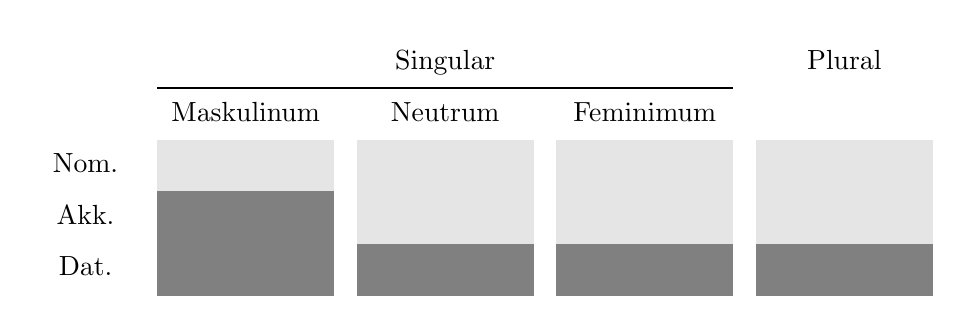
\begin{tikzpicture}
		\matrix [matrix of nodes,
		nodes in empty cells,
		column sep=3mm,
		align=center,
		nodes={text width=2cm, minimum height=1em, font=\strut},
		column 1/.style={nodes={text width=1cm}}
		]
		(matrix)
		{         & & {Singular} & & {Plural} \\
				  & Maskulinum & Neutrum & Feminimum & \\
			Nom.  & & & & \\
			Akk.  & & & & \\
			Dat.  & & & & \\
		};
		\draw (matrix-2-2.north west) -- (matrix-2-4.north east);
		\fill [fill=gray!20]
		(matrix-3-2.north west) rectangle (matrix-3-2.south east);
		\fill [fill=gray]
		(matrix-4-2.north west) rectangle (matrix-5-2.south east);
		\fill [fill=gray!20]
		(matrix-3-3.north west) rectangle (matrix-3-3.south east);
		\fill [fill=gray]
		(matrix-5-3.north west) rectangle (matrix-5-3.south east);
		\fill [fill=gray!20]
		(matrix-4-3.north west) rectangle (matrix-4-3.south east);
		\fill [fill=gray]
		(matrix-5-4.north west) rectangle (matrix-5-4.south east);
		\fill [fill=gray]
		(matrix-5-5.north west) rectangle (matrix-5-5.south east);
		\fill [fill=gray!20]
		(matrix-3-5.north west) rectangle (matrix-4-5.south east);
		\fill [fill=gray!20]
		(matrix-3-4.north west) rectangle (matrix-4-4.south east);
	\end{tikzpicture}
\caption{\label{fig:16}Synkretismuskonstellationen in den Definitartikelparadigmen}
\end{figure}

Im nordbair. Artikelsystem ist nach \citet[428]{Rowley1990b} eine dritte Synkretismuskonstellation (NAD) zu finden (vgl. \tabref{tab:40}). Neutra im Plural haben hier eine spezifische, kasussynkretische Form des Definitartikels: neutr. \textit{deiɐ ghinɐ} ‚die Kinder‘ vs. mask. \textit{die boum} ‚die Buben‘ (vgl. \teuthoo{de<E}{dêə} \teuthoo{mo<i.«d»lAn}{môiͅ(d)lαn} ‚den Mädchen‘ im nordbair. Groschlattengrün). Ein synkretischer Pluralartikel findet sich vereinzelt auch im Ofr. und (für alle Genera) im Nordbair. (vgl. \citealt[347]{Rowley2004}, \citealt[436]{SMF7}).\footnote{Z.\,B. mit betontem Artikel \teuthoo{îi“4}{{\aufstrih}ị̄} \teuthoo{mu<os}{mûos} \teuthoo{di}{di} \teuthoo{khu"?E.}{khǖəͅ} \teuthoo{vo?.dEr}{vöͅdər} ‚ich muss die Kühe füttern‘ und mit unbetontem Artikel \teuthoo{gab}{ɡab} \teuthoo{A4ma9.2}{α̣ma\klammeruntenpost{}̄ͅ} \teuthoo{dE}{də} \teuthoo{khu"?E.}{khǖəͅ} \teuthoo{wa.s}{waͅs} \teuthoo{dsu}{dsu} \teuthoo{v5ra4sE}{v̩rạsə} ‚gib einmal den Kühen was zum Fressen‘ (ofr. Erlabrunn) oder im nordbair.-mittelbair. Grafenkirchen: \teuthoo{de4}{dẹ} \teuthoo{k\_e.<i}{kʰêͅi} ‚die Kühe (kaufe ich nicht)‘ und \teuthoo{miE}{miə} \teuthoo{gemS}{ɡemʃ} \teuthoo{de4}{dẹ} \teuthoo{k\_e.<i}{kʰêͅi} ‚wir geben es den Kühen‘.}


\begin{table}[p]
\begin{tabular}{lllllll}
\lsptoprule
& \multicolumn{3}{c}{{Sg.}} & \\
 & {Mask.} & {Neutr.} & {Fem.} & \multicolumn{2}{c}{{Pl.}} & \multicolumn{1}{l}{{Neutr.}}\\\cmidrule(lr){2-4}\cmidrule(lr){5-6}\cmidrule(lr){7-7}
{Nom.} & \cellcolor{lsLightGray}\textit{dα} / \textit{deα} & \cellcolor{lsLightGray}\textit{(ə)s} / \textit{des} & \cellcolor{lsLightGray}\textit{d‘} / \textit{di} & \cellcolor{lsLightGray}\textit{d‘} / \textit{de}\footnote{Im nordbair. Groschlattengrün, wo sich keine klitisierten Artikelformen finden, lautet der unbetonte Pluralartikel \textit{di}, der betonte \textit{dei}.} & \cellcolor{lsLightGray}\textit{də} / \textit{di} & \textit{deiɐ}\\
{Akk.} & \cellcolor{lsLightGray}\textit{αn} / \textit{dαn} & \cellcolor{lsLightGray} & \cellcolor{lsLightGray} & \cellcolor{lsLightGray} & \cellcolor{lsLightGray} & \\
{Dat.} & \cellcolor{lsLightGray} & \textit{n} & \cellcolor{lsLightGray}\textit{dα} & \cellcolor{lsLightGray}\textit{(α)n} & \cellcolor{lsLightGray} & \\
\lspbottomrule
\end{tabular}
\caption{Flexionsparadigma des Definitartikels (unbetont\slash betont) im Nordbair. (vgl. \citealt[427]{Rowley1990b}). Die Paradigmen stellen eine Abstraktion der heteromorphischen Varianten dar, d.\,h. im Einzeldialekt können die Artikelformen anders realisiert werden. Grau hinterlegt sind in dieser und in den folgenden Tabellen die Paradigmenpositionen, die durch die eigenen BSA-Daten gefüllt werden konnten; die weiß hinterlegten Angaben stammen von \citet[403]{Rowley1990a}, \citet[427]{Rowley1990b} zum Nordbair. sowie \citet[316]{Eroms1989} und \citet[237]{Scheutz1988} zum Mittelbair.\label{tab:40}}
\end{table}

\begin{table}[p]
\begin{tabular}{llllll}
\lsptoprule
& {Mask.} & {Neutr.} & {Fem.} & \multicolumn{2}{c}{{Pl.}}\\\cmidrule(lr){2-4}\cmidrule(lr){5-6}
{Nom.} & \cellcolor{lsLightGray}\textit{dα} / \textit{deα} & \cellcolor{lsLightGray}\textit{əs} / \textit{des} & \cellcolor{lsLightGray}\textit{də} / \textit{di} & \cellcolor{lsLightGray}\textit{di} & \cellcolor{lsLightGray}\textit{də} / \textit{di}\\
{Akk.} & \cellcolor{lsLightGray}\textit{(α)n} / \textit{dαn} & \cellcolor{lsLightGray} & \cellcolor{lsLightGray} & \cellcolor{lsLightGray} & \cellcolor{lsLightGray}\\
{Dat.} & \cellcolor{lsLightGray} & \textit{ən} / \textit{den} & \cellcolor{lsLightGray}\textit{dα} / \textit{deα} & \textit{ən} / \textit{den} & \cellcolor{lsLightGray}\\
\lspbottomrule
\end{tabular}
\caption{Flexionsparadigma des Definitartikels (unbetont\slash betont) im Ofr. (vgl. \citealt[403]{Rowley1990a} sowie \citealt[189]{SUF3} speziell zum Unterofr.). Beim Nom.\slash Akk. der Feminina wurde in den ausgewerteten BSA-Daten jeweils nur die Form \textit{di} realisiert; hier kann allerdings auch eine unbetonte Form \textit{də} angenommen werden, die in den ofr. Ortsdialekten mit vollständigem Kasussynkretismus im Fem. im Satzkontext produziert wurde.\label{tab:41}}
\end{table}

\begin{table}[p]
\begin{tabular}{lllll}
\lsptoprule
& {Mask.} & {Neutr.} & {Fem.} & {Pl.}\\\midrule
{Nom.} & \cellcolor{lsLightGray}\textit{dα} / \textit{deα} & \cellcolor{lsLightGray}\textit{(α)s} / \textit{des} & \cellcolor{lsLightGray}\textit{d‘} / \textit{de} & \cellcolor{lsLightGray}\textit{d‘} / \textit{de}\\
{Akk.} & \cellcolor{lsLightGray}\textit{αn} / \textit{dαn} & \cellcolor{lsLightGray} & \cellcolor{lsLightGray} & \cellcolor{lsLightGray}\\
{Dat.} & \cellcolor{lsLightGray} & \textit{an} / \textit{den} & \cellcolor{lsLightGray}\textit{dα / dera} & \textit{de} / \textit{dene}\\
\lspbottomrule
\end{tabular}
\caption{Flexionsparadigma des Definitartikels (unbetont\slash betont) im Mittelbair. (vgl. \citealt[316]{Eroms1989}, \citealt[237]{Scheutz1988})}
\label{tab:42}
\end{table}

Auch wenn in den eigenen Daten hierfür keine Belege gefunden wurden, so wird in dialektologisch-grammatischen Darstellungen außerdem eine Tendenz zum Kasussynkretismus bei den Feminina für Teile des Ofr. beschrieben. \citet[Karte 6]{Shrier1965} setzt für einen Ortspunkt im Unterofr. den völligen Zusammenfall der Kasusdifferenzierung beim fem. Definit- und Indefinitartikel an, mit \textit{də} als synkretischem fem. Definitartikel. \citet[§6d]{Schübel1955} sieht den „Bestand und Bereich“ des Dativs „stark bedroht“; im ofr. Stadtsteinach findet sich die Variante \teuthoo{ic}{iX} \teuthoo{ho2us}{hōus}  \teuthoo{di}{di} \teuthoo{fra2}{frā} \teuthoo{ge2m}{ɡēm} ‚Ich hab’s der Frau gegeben‘ neben \teuthoo{ic}{iX} \teuthoo{ho2us}{hōus} \teuthoo{da?}{dä} \teuthoo{fra2}{frā} \teuthoo{ge2m}{ɡēm}. Auch \citet[92]{Rowley1997} beschreibt für dieses oberofr. Gebiet eine Entwicklung hin zu völligem Kasussynkretismus bei den Feminina. Die Varianten \teuthoo{nai}{nai} \teuthoo{di}{di} \teuthoo{windEriN}{windəriŋ} vs. \teuthoo{nai}{nai} \teuthoo{dE}{də} \teuthoo{windEriN}{windəriŋ} ‚(die Karpfen kommen) hinein die Winterunterbringung‘,\footnote{Zur Verwendung und Arealität von Lage- und Richtungsadverbien als Präpositionen im Ofr. vgl. den Forschungsüberblick und die Ergebnisse im SMF (\citealt[434--438]{SMF7}, vgl. auch \citealt{WA}-Karten 28, 56, 467 „in“).}  die sich „in kurzer Abfolge“ finden, sind \citet[92]{Rowley1997} zufolge auf die durch den Satzakzent bedingte Verwendung des betonten und des unbetonten (d.\,h. nicht akzentuierbaren) Artikels zurückzuführen. Demnach wären hier zwei unterschiedliche, aber jeweils synkretische Paradigmen anzusetzen: Nom./Akk./Dat. \textit{di} als betonter und Nom.\slash Akk./Dat. \textit{də} als unbetonter Definitartikel.

Diese beiden Reihen des Artikels, d.\,h. Vollformen vs. reduzierte Formen, müssen für alle untersuchten Dialekte angesetzt werden (vgl. 	\tabref{tab:40} bis \tabref{tab:42}). Allerdings ist die Distribution der beiden Artikelformen nicht nur durch Akzent und Position bedingt, sondern auch durch unterschiedliche Funktionalitäten im semantisch-pragmatischen Kontext (siehe hierzu
\citealt{Eroms1989}, \citealt{Scheutz1988}, \citealt{WeißDirani2019}). Im BSA-Fragebuch wurden die beiden Reihen des Definitartikels zwar berücksichtigt, etwa durch die Fragen „Die Häuser (betont!) gefallen uns nicht“ oder „Die Kühe (unbetont!) kauf‘ ich nicht“, allerdings ist das Datenmaterial außerhalb dieser elizitierten Syntagmen zu heterogen und zu wenig eindeutig, um auf die Distribution von Voll- und reduzierten Formen zu schließen.\footnote{Bedingt durch die Datenlage lassen sich daher nur einzelne Beobachtungen aufführen, da Definitartikel für einzelne Paradigmenposition gar nicht oder nur in Form eines Abfrage-Items vorliegen (vgl. die Problematisierung in \sectref{sec:7.2}). Erschwert wird die Auswertung dadurch, dass eine Klassifikation und Differenzierung nach Kasus anhand der Transkriptionen (und der wenigen Abfrage-Items) nicht immer eindeutig ist, insbesondere wenn der Artikel in der reduzierten Form vorkommt (siehe auch \citealt[189]{SUF3}). Bedingt durch die Art der Datenerhebung kommen mögliche Intervieweffekte hinzu (zumeist isolierte Antwort-Items und die Elizitierung der relevanten NPs in der Vorfeld-Position), die die Realisierung der Artikelform (Vollform oder reduzierte Form) beeinflussen.} Des Weiteren haben \citet[330]{WeißDirani2019} in ihrer Studie zum hess. Definitartikelsystem jüngst gezeigt, dass für die Funktionalität der beiden Definitartikelformen insbesondere mit Blick auf Faktoren der Informationsstruktur „a more fine-grained differentiation“ angesetzt werden muss, als bisher angenommen. Um die Distribution der Artikelformen in den Dialekten abbilden zu können, braucht es dementsprechend Datenmaterial, das die verschiedenen morphosyntaktischen und informationsstrukturellen Faktoren systematisch berücksichtigt (vgl. \citealt[239--240]{Scheutz1988}).\footnote{Siehe hierzu als Beispiel die Erhebungen des SNiB, wo die Verwendung von reduzierter vs. Vollform bei einfachen Wiederaufnahmesituationen eliziert und Spontanantworten vs. akzeptierte Antworten systematisch differenziert wurden (\citealt[130]{SNiB1}).}

In den bair. Dialekten wird die unbetonte Artikelform \textit{die} im Nominativ/Akkusativ der Feminina und des Plurals als Proklise realisiert, z.\,B. (mit Assimilation des Artikels) \teuthoo{b-mu<94AtE}{b{}͐mû\klammeruntenpost{}̣αtə} -- \teuthoo{b-mu42AtEn}{b{}͐mụ̄αtən} ‚Mutter‘ im mittelbair. Grafenau, \teuthoo{svenStA}{svenʃtα} -- \teuthoo{b,venStA}{b͓venʃtα} ‚Fenster‘ im nordbair. Nabburg (vgl. \citealt[112--114 und Karte 18]{Rowley1997}, \citealt[§449]{Schmeller1821}). Variation besteht in den Dialekten dahingehend, ob der Definitartikel auch positionsbedingt vor einem Adjektivattribut reduziert werden kann: \textit{s’laar(e)} vs. \textit{des laar(e) Glas} ‚das leere Glas‘, \textit{d’schene} vs. \textit{de schene} ‚die schöne (Huberbäuerin)‘. Dieser Aspekt wurde im Band 1 des \textit{Sprachatlas von Niederbayern} systematisch erhoben und ausgewertet, und es zeigt sich, dass bei Neutra und noch stärker bei den Feminina die Vollform gegenüber der klitisierten Form präferiert wird (\textit{de schene} vs. \textit{d’schene}), während bei den Maskulina die reduzierte Form \textit{dα oi(te)} gegenüber der Vollform \textit{deα oi(te)} ‚der alte (Bauer)‘ präferiert wird (\citealt[108--130]{SNiB1}, vgl. \citealt[317]{Eroms1989}). Auch in den untersuchten Dialekten erscheint vor Adjektivattribut eher die Vollform des Artikels als die reduzierte Form (tatsächlich findet sich kein Beleg für Artikelproklise vor Adjektiv\-attribut).

Mit Blick auf die formale Realisierung der Definitartikel und deren Distribution sind daneben auch Sandhi-Effekte zu beobachten. In Flexionssystemen, die keine Distinktion zwischen Dativ und Akkusativ im Singular des Maskulinums oder Neutrums haben, ist zum Teil eine progressive Assimilation des Definitartikels \textit{αn} > \textit{αm} zu finden (Typ \textit{Ghead des an Hans oda am Franz} ‚Gehört das dem Hans oder dem Franz‘, \citealt[09]{Zehetner1985}): Akk.Sg. \teuthoo{Am}{αm} \teuthoo{b5a4<o<n}{b̩ậôn} ‚Bauer‘ vs. Akk.Sg. \teuthoo{An}{αn} \teuthoo{s\#po.2ds}{špōͅds} ‚Spatz‘ (mittelbair. Wolfersdorf), \teuthoo{Am}{αm} \teuthoo{be4<Ag}{bệαɡ} \teuthoo{a4ofi}{ạof‌i} ‚auf den Berg hinauf‘ (mittelbair. Wolfersdorf) vs. \teuthoo{An}{αn} \teuthoo{b\%eAg}{b͈eαɡ} \teuthoo{a4u:fe}{ạu{\doubleogonek}fe} ‚auf den Berg hinauf‘ (mittelbair. Inning am Holz, vgl. \citealt[§3d]{Schübel1955}). Daneben bietet \citet[§59]{Freudenberg1959} einen Beleg dafür, dass in Flexionssystemen, in denen Akkusativ und Dativ unterschieden werden, diese Differenzierung durch Assimilation aufgehoben werden kann: mittelbair. \teuthoo{i}{i} \teuthoo{ha2sn@}{hāsn̥} \teuthoo{ge2wA}{ɡēwα} ‚ich habe es ihm gegeben‘.

\subsection{Kasusmarkierung in der Nominalphrase}\label{sec:9.1.2}
Im UG besteht Variation dahingehend, welche Kasus durch Präpositionen regiert werden. Bei den Richtungsadverbien in präpositionaler Funktion im Ofr. sind variante Kasusrektionen auch raumbildend, z.\,B \textit{hinauf der Eiche} mit Dativrektion vs. \textit{hinauf die Eiche} mit Akkusativrektion (\citealt[435--436 und Karten 121--125]{SMF7}). Grundsätzlich zu unterscheiden sind Dialektsysteme, in denen Präpositionen immer den Dativ regieren, wie es \citet[93]{Rowley1997} für die konservativen ofr. Dialekte beschreibt, und jene, in denen Akkusativ und Dativ regierende Präpositionen unterschieden werden, beispielsweise \teuthoo{a4v5}{ạv̩} \teuthoo{d5o<).AxA}{d̩ô\klammeruntenpost{}ͅαxα} ‚auf der Eiche‘ vs. \teuthoo{untA4}{untα̣} \teuthoo{dE}{də} \teuthoo{o.AxE}{oͅαxə} ‚unter der Eiche‘ im mittelbair. Grafenau. Auch im südlichen Unterofr. und dem westlichen Streifen des Ofr. werden Präpositionen mit Akkusativ- und Dativrektion unterschieden, doch erscheint in einem relativ geschlossenen Gebiet nach dativregierenden Präpositionen numerusunabhängig der Definitartikel \textit{der}: \teuthoo{An}{αn} \teuthoo{dEr}{dər} \teuthoo{hend5\_}{hend̩ʰ} ‚an den Händen‘ (ofr. Gebsattel), \teuthoo{na2}{nā} \teuthoo{BE}{{\btilde}ə} \teuthoo{dEr}{dər} \teuthoo{a.ldi}{aͅldi} \teuthoo{ho<I?sEr}{hôı̈sər} ‚nahe bei den alten Häusern‘ (ofr. Ochsenfurt), \teuthoo{mi.dEr}{miͅdər} \teuthoo{bu2Em}{būəm} ‚mit den Buben‘ (ofr. Hüttenheim, vgl. \citealt[Karte 56]{SUF3}).

Ein Beispiel für die Variabilität flexivischer Kodierung in der Nominalphrase bieten jene nordbair. und ofr. Dialekten, die eine distinkte Dativ-Plural-Form haben. Exemplarisch zeigt dies die Belegreihe \teuthoo{mitE}{mitə}
\teuthoo{g\_\i“En@}{ɡʰ̈īən̥} ‚mit der Kette‘ vs. \teuthoo{mi}{mi} \teuthoo{k\_i“ErAn}{kʰīərαn} ‚mit Ketten‘ aus dem nordbair. Windischeschenbach: Der Definitartikel entfällt, wenn eine flexivische Markierung der Kasus- und Numerusinformation am Substantiv zu Verfügung steht. In der Nominalphrase besteht also eine Tendenz zur Monoflexion, es findet eine „Arbeitsteilung der nominalflexivischen Kennzeichnung“ \citep[387]{Harnisch2019} statt: entweder am Substantiv oder am Artikel.

In Dativ regierten Präpositionalphrasen mit pluralischer Nominalphrase wird die flexivische Information in diesen Dialekten präferiert am Substantiv kodiert; der Artikel wird entweder reduziert (klitisiert) realisiert oder es erscheint kein Artikel: \teuthoo{avÑ}{av{\burgermn}} \teuthoo{ba42mana}{bạ̄mana} ‚auf den Bäumen‘ (ofr. Hallerstein), \teuthoo{in}{in} \teuthoo{a4rmAn}{ạrmαn} ‚in den Armen‘ (nordbair. Tirschenreuth), \teuthoo{a4m}{ạm} \teuthoo{ne4s5dnAn}{nẹs̩dnαn} \teuthoo{dra.n}{draͅn} ‚an den Ästen dran‘ (nordbair.-mittelbair. Blaibach). Diese Belege sind auch insofern bemerkenswert, als \citet[95]{Rowley1997} für in sein nordostbayerisches UG nach Präposition eher die Form ohne Dativ-Plural-Suffix anführt.\largerpage[2]

\begin{sloppypar}
Beispiele für morphosyntaktische Varianten nach Präposition bietet auch \citet[§13]{Schübel1955} für den ofr. Dialekt von Stadtsteinach: \textit{mid di bȳχe} -- \textit{midn bȳχenɐ} ‚mit den Büchern‘, \textit{họie šded negs auf di fäle} -- \textit{aufm fälenɐ} ‚heuer steht nichts auf den Feldern‘. Des Weiteren zeigt \citet[§13]{Schübel1955}, dass auch Kasuswechsel am Artikel in Kauf genommen wird, um Numerus eindeutig zu markieren.\footnote{Auch \citet[§12]{Weitzenböck1942} bietet Belege dafür, dass Numerusambiguitäten in der Präpositionalphrase durch eine andere Kasusmarkierung am Artikelwort aufgelöst werden: mittelbair. \teuthoo{fo}{fo} \teuthoo{ma+n}{mãn} \teuthoo{fe24dA+n}{fẹ̄dα̃n} ‚von meinem/meinen Vetter(n)‘ wird zu \teuthoo{fo}{fo} \teuthoo{ma+ne4}{mãnẹ} \teuthoo{fe24dA+n}{fẹ̄dα̃n} ‚von meinen Vettern‘ mit dem Possessivartikel im Akk.Pl., wenngleich dieser „nicht bodenständige [d.\,h. basisdialektale, GN] Ersatz aus der städtischen Sprache“ und anderen Dialekten stamme und „offenbar im Vordringen“ sei.} Im Syntagma \textit{en báuen kǫsdɒ šö dráun} ‚dem/den Bauern kannst du schon trauen‘ liegt durch den synkretischen Artikel \textit{en} (Akk./Dat.Sg.mask. und Dat.Pl.) Numerusambiguität vor, die entweder flexivisch am Substantiv oder durch den Pluralartikel des Nom./Akk. (\textit{di}) vereindeutigt wird: \textit{en báuenɒ} oder \textit{di báuen} \textit{kǫsdɒ šö dráun} ‚den Bauern kannst du schon trauen‘ (siehe auch \sectref{sec:7.2.2}). \citet[123--124]{Steininger1994} zufolge wäre im Flexionssystem des mittelbair. Oberneureutherwaid der „potenzierte Plural“ in der Form des Dat.Pl. bei der synkretischen Artikelform \textit{en} obligatorisch (\textit{bis’a én Buaman schreid} ‚bis er die Buben weckt‘), während er in einer NP mit distinktem Artikel (Dat.Sg. \textit{dän} -- Pl. \textit{dé}) „sogar ungrammatisch“ wäre: \textit{Dé Buam} (*\textit{dé Buaman}) \textit{gibd’a oiss} ‚Den Buben gibt er alles‘.
\end{sloppypar}

Während die formale Variabilität bei der Kodierung der flexivischen Information in diesen Fällen der Disambiguierung der Numerusinformation dient, hat sich im Bair. (neben anderen obd. Dialekten) eine weitere dialektspezifische Strategie zur Kodierung der Kasusinformation des Dativs herausgebildet: die präpositionale Dativmarkierung des Typs \textit{gibs α da Kathi} ‚gib es der Kathi‘. Im Mittelbair. ist bei den reduzierten Definitartikelformen des Plurals Kasusdistinktion vorhanden (Nom./Akk.Pl. \textit{d’leit} vs. Dat.Pl. \textit{de leit} ‚Leute‘), nicht aber bei den Vollformen: Nom./Akk./Dat.Pl. \textit{de leit} \citep[98--99]{Seiler2003}. \citet[150]{Seiler2003} analysiert die präpositionale Dativmarkierung als „eine Angelegenheit der Ausbuchstabierung des Dativs“, indem der Marker den Kasus der folgenden NP explizit markiert und vor dem Hintergrund einer Präferenz von Dativ in Kookkurrenz mit vorangehender Präposition heraus zu verstehen ist; der Dativmarker hat damit die „Funktion eines Expletivs, eines Platzhalters“ \citep[148]{Seiler2003}. Aus flexionsmorphologischer Perspektive ist hierbei \citegen[166]{Seiler2003} Befund zentral, dass der Dativmarker v.\,a. im Südbair. und teilweise im Mittelbair. häufiger im Plural als im Singular vorkommt, das heißt da, wo Synkretismen in der Nominalphrase vorliegen (\textit{di leit} vs. \textit{in di leit} ‚den Leuten‘). Hier hat die präpositionale Dativmarkierung eine disambiguierende Funktion.

Insgesamt erscheint der präpositionale Dativmarker im Bair. eher mit Definitartikel, so auch in einem Teil der untersuchten mittelbair. Dialekte: \teuthoo{A}{α} \teuthoo{dA}{dα} \teuthoo{mu<AtA}{mûαtα} \teuthoo{gðs5o.gd}{ɡ̩s̩oͅɡd} ‚der Mutter gesagt‘ und \teuthoo{A}{α} \teuthoo{d5e4n}{d̩ẹn} \teuthoo{o.idn}{oͅidn} \teuthoo{mo4"+}{mọ̃̄} ‚dem alten Mann (gegeben)‘ in Kirchensur (vgl. \citealt[106--110]{Seiler2003}). Seltener und unregelmäßiger verteilt ist die präpositionale Dativmarkierung nach De"-mons"-tra"-tiv-,"" Pos"-ses"-siv-"" oder In"-ter"-ro"-ga"-tiv"-ar"-ti"-kel, z.\,B. \teuthoo{A}{α} \teuthoo{de4<}{dệ} \teuthoo{we4<cAn}{wệXαn} \teuthoo{k\_i."4ndA}{kʰị̄ͅndα} ‚welchen Kindern (hast du es gegeben)‘ in Reischach. Das Auftreten des Dativmarkers ist dabei „mehr oder weniger optional“ \citep[152]{Seiler2003}, {{dativische}} Nominalphrasen kommen etwa im mittelbair. Niedertaufkirchen auch ohne präpositionalen Dativmarker vor: \teuthoo{A}{α} \teuthoo{dA}{dα} \teuthoo{mu.<AtAn}{mûͅαtαn} \teuthoo{ks5o.k,t,\_}{ks̩oͅk͓t͓ʰ} ‚der Mutter gesagt‘ vs. \teuthoo{de4n}{dẹn} \teuthoo{o4<e4dn@}{ộẹdn̥} \teuthoo{ma.>(+}{mẫͅ\klammerobenpost{}} ‚dem alten Mann (gegeben)‘. Grundsätzlich ist das Auftreten der präpositionalen Dativmarkierung an keine semantischen Distinktionen gekoppelt, sie kodiert keine semantischen Rollen. Nach \citet[187]{Seiler2003} stellen aber informationsstrukturelle Aspekte in den Dialekten mit optionaler präpositionaler Dativmarkierung einen Auftretensfaktor dar: „Je mehr eine dativische NP diskursfunktional markiert ist, desto eher wird sie präpositional markiert.“

Diese Zusammenschau an Phänomenen zeigt, dass sich in den dialektalen Flexionssystemen spezifische Strategien zur Vereindeutigung von Numerus- oder Kasusinformation finden, die erst im morphosyntaktischen Kontext greifen. Im Falle der präpositionalen Dativmarkierung sind diese sogar grammatikalisiert. Vor dem Hintergrund von Numerusprofilierung und Kasusnivellierung als zentralen Tendenzen nominalmorphologischen Wandels ist gleichzeitig bemerkenswert, dass in einzelnen Dialektsystemen Kasuswechsel des Artikels in Kauf genommen werden, um eine eindeutige Kodierung der Numerusinformation sicherzustellen. Insgesamt entsprechen die dialektalen Strategien im UG auch der Beobachtung \citegen[436]{Shrier1965}, dass (morpho-)syntaktische Ambiguitäten als Folge von Synkretismen durch weiteren Kontext und kommunikative Strategien disambiguiert werden.

\section{Systematische Variation der Pluralmarkierung im syntaktischen Kontext}
\label{sec:9.2}
In den Kapiteln zur Formenbildung und zum dialektalen Deklinationsklassensystem wurde punktuell immer wieder vermerkt, dass die eine oder andere distinkte Markierung in dialektologisch-grammatischen Darstellungen als fakultativ (d.\,h. als optional) klassifiziert wurde:

\begin{itemize}
\sloppy
\item Im mittelbair. Dialekt von Oberneureutherwaid erscheinen keine Lenis-Fortis-Kontraste als Mittel der Numerusdifferenzierung, wenn der Plural bereits durch ein Zahlwort ausgedrückt wird: \textit{d̥iːʒ} -- \textit{d̥iʃ} ‚Tisch‘, aber \textit{t̥sβæ d̥i:ʒ} ‚zwei Tische‘ (\citealt[124]{Steininger1994}, siehe \sectref{sec:7.1.2.3.1}). Nach Zahlwort besteht nach \citet[105]{Rowley1997} grundsätzlich „die morphosyntaktische Option“, die unflektierte Form des Nom.Sg. zu verwenden, und zwar unabhängig von einer Semantik des Lexems als Maß- und Mengenangabe und vom jeweiligen Pluralmarkierungsverfahren (vgl. \sectref{sec:8.3.2}).
\item Im südlichen Nordbair. ist die additive Markierung durch Nasalsuffix von Maskulina mit Tiefschwa- und \textit{el}{}-Reduktionssilbe fakultativ (daneben auch bei Diminutiva auf -\textit{el}), wenn „der syntaktische Rahmen keine weiteren Hinweise auf die Pluralität liefert“ \citep[158]{Rowley1997} und der Stammvokal im Plural keinen Umlaut aufweist: Pl. \teuthoo{s\#lisln}{šlisln} vs. \teuthoo{tswaI2\textsuperscript{n}}{tswaı̄\textsuperscript{n}} \teuthoo{s\#lisl}{šlisl} ‚zwei Schlüssel‘ (\citealt[421]{Schirmunski1962}, siehe \sectref{sec:8.3.3.1}).
\item Gleichermaßen ist laut \citet[158]{Rowley1997} auch die Pluralmarkierung der Feminina mit \textit{n}{}-Erweiterung im Nom.Sg. im südlichen Nordbair. fakultativ, daneben finden sich Belege für das Mittelbair., etwa bei \citet[§140.7]{Kollmer1987}: \teuthoo{a}{a} \teuthoo{ha.fa}{haͅfa} \teuthoo{s\#ne-gwad.n}{šne{}͐ɡwadͅn} ‚ein Haufen Schneewehen‘ vs. \teuthoo{s\#negwa.dna}{šneɡwaͅdna} \teuthoo{ho.ds}{hoͅds} \teuthoo{do.}{doͅ} \teuthoo{ge2m}{ɡēm} ‚Schneewehen hat es da gegeben‘, \teuthoo{zw.ou}{zwͅou} \teuthoo{no.dan}{noͅdan} ‚zwei Nattern‘ vs. \teuthoo{I}{ı} \teuthoo{veacht}{veaXht} \teuthoo{d}{d} \teuthoo{no.dana}{noͅdana} \teuthoo{ne2d}{nēd}! ‚Ich fürchte die Nattern nicht‘.
\item Eine zusätzliche formale Markierung erfolgt im Dat.Pl., wenn die Numerusinformation infolge von Artikelsynkretismen nicht disambiguiert wird (mittelbair. \teuthoo{mim}{mim} \teuthoo{bu2Am}{būαm} ‚mit dem/mit den Buben‘ neben Dat.Pl. \teuthoo{mim}{mim} \teuthoo{bu2AmA+n}{būαmα̃n}, \citealt[§12]{Weitzenböck1942}) oder wenn nach Präposition kein Artikel realisiert wird: Sg. \teuthoo{mitE}{mitə} \teuthoo{g\_i“En@}{ɡʰīən̥} ‚mit der Kette‘ vs. Pl. \teuthoo{mi}{mi} \teuthoo{k\_i“ErAn}{kʰīərαn} im nordbair. Windischeschenbach (vgl. Abschnitte~\ref{sec:7.2.2} und \ref{sec:9.1}). \citet[124]{Steininger1994} zufolge wäre der sogenannte potenzierte Plural dann ungrammatisch, wenn kein Formensynkretismus im Artikel vorliegt.
\end{itemize}

Der gemeinsame Nenner dieser fakultativen Markierungen ist jeweils die Dis"-am"-bi"-gu"-ie"-rung der Numerusinformation, indem der Plural durch ein zusätzliches Flexiv am Substantiv vereindeutigt wird. „Daß Kommunikationserfordernisse auf die Morphologie Einfluß nehmen“ \citep[124]{Steininger1994}, ist als flexivisches Prinzip im Bair. grammatikalisiert: Wenn der semantisch-pragmatische oder der syntaktische Kontext keine eindeutige Numerusinformation enthält, wird die Pluralinformation am Substantiv kodiert (vgl. \citealt[171]{Rowley1997}).

Lassen sich die semantisch-pragmatischen und syntaktischen Kontextbedingungen näher definieren, die eine explizite Markierung der Pluralinformation am Substantiv lizensieren? Einzelne Belege in den BSA-Daten zeigen, dass eine dis"-tink"-te Markierung bei isoliert realisierten Pluralformen erfolgt, während im Kontext einer Nominalphrase mit Definitartikel hingegen Nullplural erscheint, beispielsweise bei \textit{Baum}: \teuthoo{ba42m}{bạ̄m} -- \teuthoo{ba42mA94}{bạ̄mα\klammeruntenpost{}̣} -- \teuthoo{a9.n}{a\klammeruntenpost{}ͅn} \teuthoo{di.}{diͅ} \teuthoo{ba42m}{bạ̄m} im ofr. Burgbernheim\footnote{Gleichen Typs sind die Belege im ofr. Hüttenheim und im mittelbair. Wolfersdorf.} oder -- mit Umlautplural -- \teuthoo{ba4m}{bạm} -- \teuthoo{ba\$im}{ba̤im} -- \teuthoo{o.n}{oͅn} \teuthoo{dene}{dene} \teuthoo{ba4m}{bạm} im nordbair. Nabburg. Der historische \textit{i}{}-Stamm \textit{Baum} gehört nach \citet[168]{Rowley1997} zu den wenigen Substantiven, die in den rezenten Dialekten zu mehreren Deklinationsklassen gehören können (vgl. \citealt[§797]{Schmeller1821}). Bedingt durch den Zusammenfall der Diphthongreihe mhd. \textit{ei}{}-\textit{öu}{}-\textit{ou} zu \teuthoo{a.}{aͅ} erscheinen regelmäßig lautgesetzliche Nullplurale (Typ \teuthoo{ba2m}{bām} -- \teuthoo{ba2m}{bām}), daneben finden sich im Nordbair. analoge Umlautplurale sowie im Ofr. und Mittelbair. additive Markierungen durch Tiefschwa (Typ \teuthoo{ba2m}{bām} -- \teuthoo{ba2mA}{bāmα}, vgl. \sectref{sec:8.2.1}). In jenen Dialektsystemen, in denen Nullplural und gleichzeitig eine dis"-tink"-te Pluralform zur Verfügung stehen, ist die Wahl der Variante laut \citet[168]{Rowley1997} „nicht selten“ durch „pragmatische Faktoren“ gesteuert, d.\,h. durch die Eindeutigkeit der Pluralinformation im semantisch-pragmatischen und morphosyntaktischen Kontext.

Einen weiteren Beleg von Variation zwischen isolierter Pluralform und jener im syntaktischen Kontext liefert die Gewährsperson im ofr. Pfofeld. Zusätzlich zu der im BSA-Fragebuch als Syntagma abgefragten Pluralform von \textit{Bank} produzierte die Gewährsperson den Plural isoliert und realisierte da eine numerusdistinkte Variante mit Nasalsuffix (\teuthoo{be.Nk\_}{beͅŋkʰ} -- \teuthoo{be.NgN}{beͅŋɡŋ}), in der Nominalphrase mit Definitartikel und Adjektivattribut liegt hingegen Nullplural vor (\teuthoo{he.m}{heͅm} \teuthoo{di.}{diͅ} \teuthoo{a.l.dn}{aͅlͅdn} \teuthoo{be.Ng}{beͅŋɡ} \teuthoo{i.n}{iͅn} \teuthoo{dA}{dα} \teuthoo{s\#du.m}{šduͅm} ‚sie haben die alten Bänke in der Stube‘).


\begin{figure}
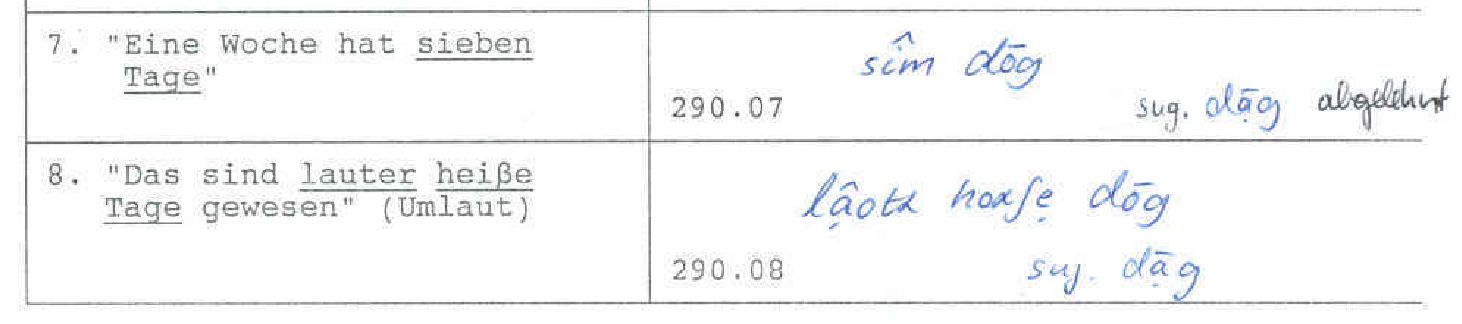
\includegraphics[width=\textwidth]{figures/Fragekontext.png}
\caption{Fragekontext \textit{Tage} im BSA-Fragebuch (nordbair.-mittelbair. Zwiesel)}
\label{fig:17}
\end{figure}

Während diese wenigen Fälle von formaler Variation bei \textit{Baum} und \textit{Bank} Zufallsfunde waren, ermöglichen die BSA-Materialien eine systematische Analyse variierender Pluralformen des Maskulinums \textit{Tag}. Auch hier liegt Variation zwischen Null- und distinkter Markierung vor, etwa in Bernried im nordbair.-mittelbair. Übergangsgebiet: \teuthoo{A}{α} \teuthoo{so4<}{sộ} \teuthoo{A}{α} \teuthoo{s\#e"+nA}{šẽ̄nα} \teuthoo{do<g}{dôɡ} ‚ein so ein schöner Tag‘ -- Pl. \teuthoo{da42g}{dạ̄ɡ} vs. \teuthoo{si."4m}{sị̄ͅm} \teuthoo{do9.<g}{do\klammeruntenpost{}̂ͅɡ} ‚sieben Tage‘. Bemerkenswert sind dabei die Antworten der Gewährsperson aus Zwiesel, ebenfalls nordbair.-mittelbair. Übergangsgebiet. Im Fragekontext ‚lauter heiße Tage‘ hat sie Nullplural produziert und die suggerierte Form mit Umlaut akzeptiert, im Kontext ‚sieben Tage‘ hat sie ebenfalls Nullplural produziert, die suggerierte Umlautform \teuthoo{da24g}{dạ̄ɡ} aber abgelehnt (\figref{fig:17}). Eine Auswertung dieser beiden Fragekontexte in allen SNiB-Erhebungsorten (n= 209) ergibt zwar in diesem Teil des Mittelbair. keine Raumbildung des Phänomens, zeigt aber zwei Haupttypen auf: (1) in beiden Fragekontexten eine „konstante“ Pluralform (Null oder Umlaut oder beide Verfahren als Varianten, 57\,\%).\footnote{Im Einzelnen setzt sich dieser „konstante“ Typus folgendermaßen zusammen: Mehrheitlich ($n=101$, 48\,\%) erscheint Nullplural in beiden Abfragekontexten, sieben Umlautplurale in beiden Kontexten (3\,\% aller Fälle), in zwölf Fällen wurde in beiden Abfragekontexten Null- und Umlautplural realisiert (6\,\%).} (2) Die Gewährsperson produziert oder akzeptiert den Umlautplural nur für die NP ‚lauter heiße Tage‘, in ‚sieben Tage‘ erfolgt Nullmarkierung (40\,\%). (In nur vier Fällen wird Umlautplural im Kontext ‚sieben Tage‘ und Nullplural bei ‚lauter heiße Tage‘ realisiert, <2\,\%.)

Die Verteilung der Varianten des Typs (2) legt hier den Schluss nahe, dass nach Numeralia Nullplural, im Syntagma ‚lauter heiße Tage‘ aber eine dis"-tink"-te Pluralform mit Umlaut realisiert wird. Allerdings hat auch das Adjektivattribut \textit{lauter} eine pluralische Semantik, weshalb sich hier erneut die Frage stellt: Welche semantisch-pragmatischen Kontexte triggern eine dis"-tink"-te Pluralform und wann sind sie (aus Sprecher/Hörer-Perspektive) eindeutig? An dieser Stelle sind die Varianten aus dem mittelbair. Wolfersdorf aufschlussreich. Als isolierte Pluralform realisiert die Gewährsperson den Umlautplural \teuthoo{da42g}{dạ̄ɡ}, im Syntagma ‚lauter heiße Tage‘ hingegen erscheint Nullplural: \teuthoo{la4otA}{lạotα} \teuthoo{ho.ASe4}{hoͅαʃẹ} \teuthoo{do.2g}{dōͅɡ} (die NP mit Zahlwort ist nicht transkribiert).

Da in den BSA-Erhebungen nur zwei Kontexte systematisch abgefragt wurden, muss offenbleiben, wo die Grenze für eine eindeutige vs. uneindeutige Interpretation von Pluralität im semantisch-pragmatischen Zusammenhang liegt. Auch in jenen bair. Dialekten, die in der Datenauswertung in beiden Kontexten (nach Zahlwort und im Syntagma ‚lauter heiße Tage‘) Nullplural haben, kann es potenziell eine fakultative Pluralmarkierung geben; die Semantik von \textit{lauter} war womöglich zu eindeutig, um diese auszulösen. Die Zusammenschau der bisherigen Fälle kontextbedingter formaler Markierung zeigt aber, dass eine dis"-tink"-te Pluralmarkierung bei isolierten Formen oder in Nominalphrasen ohne Artikel erscheint, die formale Markierung also vor allem durch fehlenden morphosyntaktischen Kontext lizensiert ist.

Um ähnliche Forschungsfragen an der Schnittstelle zwischen Flexionsmorphologie und semantisch-pragmatischem Kontext zu beantworten, braucht es weitere Dialektdaten, die (1) die Kontextbedingungen fakultativer Markierungen ausloten, (2) die Möglichkeiten von Face-to-Face-Kommunikation stärker berücksichtigen, als es in einer Interviewsituation möglich ist, und (3) inventarisieren, für welche Substantive eine fakultative Markierung überhaupt zur Verfügung steht. Der historische \textit{a}{}-Stamm \textit{Tag} und der \textit{i}{}-Stamm \textit{Baum} weisen beide lautgesetzlichen Nullplural auf (bei \textit{Baum} durch Zusammenfall der Diphthongreihe mhd. \textit{ei}{}-\textit{öu}{}-\textit{ou} zu \teuthoo{a.}{aͅ}), sie sind diachron in andere (stammaffizierende) Verfahren gewechselt. Sind Deklinationsklassenwechsel hier eine Vorbedingung für die Möglichkeit fakultativer Markierung? Im Falle stammaffizierender Markierung ist dies mit Blick auf die (dürftige) Datenlage nicht auszuschließen. Anders liegt der Fall bei additiven Markierungen, vor allem bei dem im Bair. produktiven Tiefschwa-Suffix (Typ \teuthoo{ba2m}{bām} -- \teuthoo{ba2mA}{bāmα}). Bei \citet[138]{Rowley1997} und \citet[123]{Steininger1994} finden sich Belege für eine fakultative Markierung von \textit{Bube} (\textit{bouma} neben \textit{boum}), \citet[149]{Wildfeuer2001} nennt die Maskulina Akk.Pl. \textit{šręŋαn} ‚Schragen‘ und Akk.Pl. \textit{okßnα} ‚Ochsen‘, die trotz dis"-tink"-ter Artikelformen eine potenzierte Pluralmarkierung aufweisen. Er interpretiert dies als „inter- und intraparadigmatische[n] Ausgleich“, der „zukünftig mehr Wörter erfassen und schließlich regelhaft werden“ könnte (\citealt[149]{Wildfeuer2001}, vgl. \citealt[72]{Mauser2007}).

In dialektologisch-grammatischen Darstellungen wird die fakultative Markierung als besonders frequent bei Feminina mit \textit{n}-Erweiterung im Nom.Sg. angeführt (Typ \teuthoo{das\#n}{dašn} -- \teuthoo{das\#n}{dašn} ‚Tasche‘), da hier auch der Artikel im Nom./Akk. (\textit{die} -- \textit{die}) keine Dis\-am\-bi\-gu\-ie\-rung der synkretischen Numerusformen leistet. \citet[174]{Rowley1997} verortet den arealen „Kern“ der fakultativen Suffigierung von Feminina außerhalb seines nordostbayerischen UGs im Mittelbair. \mapref{map:33} bestätigt dies und zeigt, dass das Gebiet fakultativer Markierung weite Teile des Mittelbair. umfasst und -- so ist zu vermuten -- bis ins östliche Mittelbair. in Österreich hineinreicht (siehe auch \citealt{Mauser2007}).

\begin{map}
\includegraphics[width=\textwidth]{figures/Karte33.png}
\caption{Fakultative („potenzierte“) Pluralmarkierung bei ‚Glocke‘ in den Daten des SNOB, SNiB und SOB}
\label{map:33}
\end{map}

Kartiert wurden zwei Fragekontexte aus den bair. Teilprojekten SNOB, SNiB und SOB: (1) ‚Wir brauchen neue Glocken‘ und (2) -- mit unbestimmtem Zahlwort -- ‚Man tut mit allen Glocken läuten‘. Das Kartenbild zeigt, dass Nullmarkierung in beiden Kontexten im gesamten UG, d.\,h. im Ofr. und im Bair., belegt und im interdialektalen Vergleich damit ausgesprochen frequent ist. Am nördlichen und südlichen Rand sind nu"-me"-rus"-dis"-tink"-te Formen mit apokopiertem Singularstamm zu finden (Typ \teuthoo{glok}{ɡlok} -- \teuthoo{glokN}{ɡlokŋ}). Ein Spezifikum des mittelbair.-schwäb. Übergangsgebiets im Westen des UGs ist daneben die nu"-me"-rus"-dis"-tink"-te Form mit Suffixalternation: Typ \teuthoo{glokE}{ɡlokə} -- \teuthoo{glokA}{ɡlokα} (siehe \sectref{sec:7.1.1.4}). Im östlichen Mittelbair. und im südlichen Nordbair. finden sich Belege für additive Pluralformen in beiden Fragekontexten (Typ \teuthoo{glokN}{ɡlokŋ} -- \teuthoo{glokNA}{ɡlokŋα}). Ein weitaus größeres Gebiet des Mittelbair. umfassen dagegen die fakultativen Plurale: Eine additive Pluralform findet sich nur in (1), in der NP mit unbestimmtem Zahlwort in (2) ist Nullplural realisiert, z.\,B. \teuthoo{na4ee4}{nạeẹ} \teuthoo{glo4gðnA}{ɡlọɡ̩nα} vs. \teuthoo{mid}{mid} \teuthoo{a.le4}{aͅlẹ} \teuthoo{glo4gðn@}{ɡlọɡ̩n̥} \teuthoo{le.2dn@}{lēͅdn̥} im nordbair.-mittelbair. Blaibach.

In beiden Abfragekontexten erscheint \textit{Glocke} nicht in der Subjektposition, was auch den prototypischen Fall von fakultativen Pluralmarkierungen darstellt. \citet[124]{Steininger1994} findet in seinem Korpus potenzierte Pluralformen vor allem im Akkusativ, im Nominativ gelten sie dagegen „nur mit Einschränkung, da die in der finiten Verbform geforderte Kongruenz ebenfalls die grammatische Kategorie Numerus zum Ausdruck bringt“ (vgl. \citealt[§140.7]{Kollmer1987}, \citealt[159]{Rowley1997}). In den BSA-Daten findet sich indes ein weiterer Beleg fakultativer Markierung, der diese Beobachtung herausfordert. In Bernhardswald (nordbair.-mittelbair. Übergangsgebiet) markiert die Gewährsperson den isolierten Plural von \textit{Sohle} mit Tiefschwa-Suffix (\teuthoo{so24îln}{sọ̄{\aufstrih}ln} -- \teuthoo{so24îlnA}{sọ̄{\aufstrih}lnα}) und bietet für den Satz ‚Beide Sohlen sind hin‘ zwei Varianten: \teuthoo{dso24îlnA}{dsọ̄{\aufstrih}lnα} \teuthoo{sa4n}{sạn} \teuthoo{hi“4}{hị̄} ‚die Sohlen sind hin‘ und \teuthoo{dso24îln}{dsọ̄{\aufstrih}ln} \teuthoo{sa4n}{sạn} \teuthoo{a.îl}{aͅ{\aufstrih}l} \teuthoo{dswôo.u}{dsw{\aufstrih}oͅu} \teuthoo{hi“4}{hị̄} ‚die Sohlen sind alle zwei hin‘. In beiden Fällen dis"-am"-bi"-gu"-iert die Kongruenz zum Verb die Numerusinformation, doch nur in Kombination mit dem Zahlwort entfällt die dis"-tink"-te Markierung am Substantiv. Da es sich um einen einzelnen Beleg\footnote{Das
    Syntagma ‚Beide Sohlen sind hin‘ ist zwar in mehreren BSA-Projekten abgefragt worden, aber bedauerlicherweise liegen die Daten nicht vollständig (bzw. mit fehlerhafter Zuordnung) in der \textit{BayDat} vor, weshalb eine systematische Auswertung ohne Hinzuziehung aller Fragebücher (und idealiter auch der Tonbandaufnahmen) an dieser Stelle möglich ist.}
handelt, ist es nicht unproblematisch, hier grundsätzlich auf die funktionale Bedeutung der Verbkongruenz zur Dis"-am"-bi"-gu"-ie"-rung von Pluralität zu schließen, zumal eventuell auch Intervieweffekte eine Rolle spielen. Der Beleg eröffnet aber in jedem Fall die Frage, ob die Kongruenz zwischen Subjekt-NP und Verb aus Sprecherperspektive ausreichend dis"-am"-bi"-gu"-ie"-rend wirkt oder ob die Pluralität präferiert im nominalen Bereich angezeigt wird. Um Fragen wie diese zu überprüfen, braucht es Erhebungsdaten, die fakultative Markierungen evozieren und neben semantisch-pragmatischen auch noch stärker syntaktische Bedingungen in den Blick nehmen.

\chapter{Diskussion: \textit{Where’s morphology?}}
\label{chap:10}
Wenngleich die Darstellung der Untersuchungsergebnisse in den vorangegangenen Kapiteln primär deskriptiv ausgerichtet war, wurden bereits einige Aspekte thematisiert, die stärker im sprachtheoretischen Rahmen der Arbeit zu verorten sind. Zentral war hier vor allem das Verhältnis von Form und Funktion. In \chapref{chap:7} bestand die methodische Schwierigkeit in der Abgrenzung, wann eine innerparadigmatische Alternation rein phonologisch bedingt ist und wann sie genuin morphologisch ist, d.\,h. funktionalisiert und evtl. sogar produktiv. Eine (zumindest vorläufige) Lösung dieses methodischen Problems war die Einbeziehung der mentalen Repräsentation: Gibt es überhaupt Alternationen, die rein phonologisch bedingt sind und die für die Sprecher/Hörer keinerlei morphologische Information symbolisieren? Sämtliche Alternationen wurden daher grundsätzlich im Phänomenbereich der Morphologie verortet und aus der Perspektive morphologischer Kodierung beschrieben. Inwiefern diese Lösung auch außerhalb der spezifischen Herausforderungen der Datenklassifikation tragfähig und plausibel mit Blick auf die kognitive Verankerung von Pluralmarkern ist, ist unter anderem Thema des folgenden Kapitels.

Die empirischen Befunde werden dabei nicht noch einmal im Detail dargestellt, sondern sie werden gebündelt und unter Einbeziehung von morphologischer Theoriebildung diskutiert. Die Diskussion knüpft dabei an die Leitfrage von Teil~\ref{part:II} an: „Where’s morphology?“ Grundlegend ist wieder das Verständnis von Flexion als grammatischem Schnittstellenphänomen, das heißt, nicht nur das isolierte Wort, sondern auch der morphosyntaktische und semantisch-pragmatische Kontext werden in die Überlegungen einbezogen. Im Einzelnen geht es um folgende Aspekte:

\begin{itemize}
\item In welchem Verhältnis stehen Form und Funktion, und zwar in den rezenten Flexionssystemen sowie diachron in der Entwicklung der Deklinationsklassen?
\item Wo ist Flexionsmorphologie im mentalen Lexikon zu verorten?
\item Inwiefern ist Flexionsmorphologie an andere Systemebenen gekoppelt?
\item Wie können Variabilität in der formalen Realisierung und fakultative Markierung in einem Grammatikmodell berücksichtigt werden?
\end{itemize}

\begin{sloppypar}
Ziel ist es, die dialektalen Flexionssysteme vor dem Hintergrund der theoretischen Ansätze zu vergleichen und durch die Anwendung der morphologischen Theorien auf dialektale Daten gleichzeitig deren Validität und explanatives Potenzial zu überprüfen. Die Diskussion bezieht sich dabei auf die in \chapref{chap:5} vorgestellten Modelle: \sectref{sec:10.1} fokussiert die Form-Funktions-Ebene aus Perspektive der Natürlichen Theorie, in \sectref{sec:10.2} wird dieser Aspekt vor dem Hintergrund der Vorhersagen des Relevanzprinzips diskutiert. \sectref{sec:10.3} und damit das gebrauchsbasierte Schema-Modell nach \citet{Köpcke1993} bilden schließlich Abschluss und Schwerpunkt des Kapitels.
\end{sloppypar}

\section[head=Natürliche Morphologie]{Natürliche Morphologie: Flexion zwischen optimaler Kodierung und Redundanz}
\label{sec:10.1}
Die Voraussage der Natürlichen Morphologie ist, dass sich (unter der Prämisse von Morphologie als geschlossenem, autonomen System) optimale morphologische Kodierungen herausbilden. Optimale Kodierungen sind nach \citet[22]{Mayerthaler1981} „konstruktionell ikonisch, uniform und transparent“, das heißt, sie entsprechen dem Prinzip „one function -- one form“ und ein semantisches „Mehr“ wird auch durch ein formales „Mehr“ ausgedrückt (ausführlicher \sectref{sec:5.1}). Die dialektalen Flexionssysteme des Oobd. unterlaufen dieses Ideal optimaler morphologischer Kodierungen, indem es ausgeprägte Allomorphie und eine Tendenz zu kumulativer Markierung gibt (die beide das Ideal „one function -- one form“ unterlaufen). Gleichzeitig widersprechen der hohe relative Anteil von rein stammaffizierenden Markierungen und Nullpluralen dem Ideal der konstruktionellen Ikonizität, die graduell beschrieben wird.  \figref{fig:18} zeigt exemplarisch für das nordbair. Nabburg, dass die untersuchten Dialekte das gesamte Spektrum von maximal und minimal ikonischen bis hin zu nicht- und kontra-ikonischen Kodierungen abdecken (in Form innerparadigmatischer Konsonantismusalternationen des Typs K/0).


\begin{figure}%10.1
\begin{tikzpicture}\footnotesize
		\matrix (hierarchy)
		[matrix of nodes, 
		nodes in empty cells,
		nodes={text width=2.8cm, align=center},
		row sep=.2cm
		]
		{
			& & & \\[0.1ex]
			maximal ikonsch & minimal ikonisch & nicht-ikonisch & kontra-ikonisch \\
			b{\aufstrichOgonek}ǫu – b{\aufstrichOgonek}ǫum ,Bub` & v\=iš – viʃ̌ ,Fisch` & hēvα – hēvα ,Hafen` & lōαb – l\^{ǫ}i ,Laib`\\
			biəkɑ – biəkɑn ,Birke` & haud – hait ,Haut` & ạntn̥ – ạntn̥ ,Ente` & mōαd – mōi ,Magd`\\
		};
		\draw [left color=black, 
		right color=white]
		(hierarchy-1-1.north west) rectangle (hierarchy-1-4.south east);
	\end{tikzpicture}
\caption{\label{fig:10.1}Hierarchie des konstruktionellen Ikonismus (Beispiele aus dem nordbair. Nabburg)}
\label{fig:18}
\end{figure}

In Teilen kann dieser Befund durch lautgesetzlichen Wandel erklärt werden, daneben spiegelt die Formenbildung der rezenten Dialekte das Ineinandergreifen phonologischer und morphologischer Prozesse wider. Durch die Apokope des Schwa-Suffixes entfällt in den Dialekten des UGs zunächst ein maximal ikonisches Verfahren. Die „Störungen“ \citep[43]{Mayerthaler1981} des konstruktionellen Ikonismus, die die Phonologie hier verursacht hat, werden gleichzeitig durch lautgesetzlichen, d.\,h. ebenfalls phonologischen Wandel kompensiert und zum Teil von der Morphologie funktionalisiert: Durch Einsilberdehnung, den Diph"-thong"-wech"-sel bei mhd. \textit{ei} und mittelbair. Konsonantenschwächung entstehen lautgesetzlich innerparadigmatische Kontraste der Vokalquantität, -qualität und des Konsonantismus und damit minimal ikonische Kodierungen, die zumindest eingeschränkt produktiv sind (vgl. \citealt[98]{Harnisch2016}, \citealt[43--44]{Rowley1997}). Im Falle von Subtraktion und K/0-Alternationen führen Lenisierungen sogar zu kon"-tra-""i"-ko"-ni"-schen Symbolisierungen. Die Frage ist nun: Warum halten sich diese weniger als maximal ikonischen Symbolisierungen seit Jahrhunderten weitestgehend im Paradigma? Und inwiefern sind rein stammaffizierende Markierungen tatsächlich weniger optimale Kodierungen einer morphologischen Kategorie?

\begin{sloppypar}
Eine Lösung dieser Fragen findet sich in späteren Arbeiten zur Natürlichen Morphologie, die die Prinzipien der Natürlichen Morphologie und sprachökonomischen Ansätze integrieren (ausführlicher \sectref{sec:5.1}). \citet{Harnisch1988} etwa ergänzt das Streben nach optimaler Kodierung um „kognitionsökonomische“ Prinzipien. Die lexikalische Speicherung von irregulären oder suppletiven Flexionsformen ist kognitiv vorteilhaft und ökonomischer, da auf tokenfrequente Formen schneller zugegriffen werden kann. Morphologische Irregularität ist gleichzeitig ein „Differenzierungsverfahren“ \citep[185]{Nübling2004}, da der Erhalt irregulärer Flexionsformen Synkretismen im Flexionsparadigma und damit nicht-ikonische Kodierungen verhindert. Nicht-segmentierbare, d.\,h. minimal ikonische oder kontra-ikonische Markierungen, symbolisieren die morphologische Information damit per se nicht schlechter, sondern nur anders (siehe auch \citealt{BybeeNewman1995} und \citealt[379]{Harnisch2000}).
\end{sloppypar}

Herausgefordert werden die Vorhersagen der Natürlichen Morphologie da, wo die Morphologie zu „Störungen“ des konstruktionellen Ikonismus und zur Aufhebung morphologischer Distinktionen führt: durch die Generalisierung des Nasalsuffixes im Paradigma der Feminina des Typs \teuthoo{das\#n}{dašn} -- \teuthoo{das\#n}{dašn} ‚Tasche‘, die auf innerparadigmatischen, morphologischen Ausgleich zurückgeht. Und auch die kumulativen (und damit nicht-optimalen) Markierungen in \teuthoo{s\#du.2m}{šdūͅm} -- \teuthoo{ds\#di"mA}{dšdīmα} ‚Stube‘ und \teuthoo{o4<b5v5l°@}{ộb̩v̩l̥̑} -- \teuthoo{epfl°@n@}{epf‌l̥̑n̥} ‚Apfel‘ (nordbair.-mittelbair. Bernhardswald) sind nicht das Ergebnis phonologischer Prozesse, sondern sekundärer morphologischer Markierungen (vgl. \sectref{sec:8.3.3.1}).

Dass kumulative Markierungen durch Morphologie geschaffen werden, kann das Konzept der Systemangemessenheit nach \citet{Wurzel1984} erklären. Im südlichen Nordbair. wird eine additive Pluralmarkierung mit Nasal- oder Tiefschwa-Suffix durch eine prosodische Input-Konditionierung bei Maskulina und Feminina auf Reduktionssilbe mhd. -\textit{el}, -\textit{en}, -\textit{er} gefordert. Im Tiefenbohrungspunkt Bernhardswald tritt die Suffigierung auch an Stämme, die bereits Umlautplural aufweisen: Pl. \teuthoo{ds\#di"mA}{dšdīmα} ‚Stuben‘, \teuthoo{ds\#na\$wl°@n@}{dšna̤wl̥̑n̥} ‚Schnäbel‘, \teuthoo{epfl°@n@}{epf‌l̥̑n̥} ‚Äpfel‘. Hier wäre die fehlende Suffigierung nicht systemangemessen, auch wenn dies zu einer redundanten, kumulativen Markierung der Pluralinformation führt (vgl. \citealt[99]{Harnisch2016}, \citealt[43]{Rowley1997}).

\begin{sloppypar}
Während minimal und kontra-ikonische Formen genauso wie kumulative Markierungen durch die Berücksichtigung von Systemangemessenheit und Ge"-brauchs"-fre"-quenz mit den (erweiterten) Annahmen der Natürlichen Morphologie durchaus in Einklang gebracht werden können, bleibt die Frage: Wie wird der hohe Anteil von Nullpluralen insbesondere bei den Feminina im nördlichen Nordbair. und im Ofr. erklärt? Die morphologische Kategorie wird hier auch nicht durch den Artikel kodiert, da Formensynkretismus vorliegt (\teuthoo{di}{di} \teuthoo{das\#n}{dašn} -- \teuthoo{di}{di} \teuthoo{das\#n}{dašn}). Während sich in einem Teil des Bair. eine ikonische, additive Markierung des Typs \teuthoo{das\#nA}{dašnα} herausgebildet hat, die sogar auf einige Maskulina analogisch übertragen wird (\textit{boumα} ‚Buben‘, \textit{okßnα} ‚Ochsen‘, vgl. \citealt[149]{Wildfeuer2001}), halten sich im Ofr. die fem. Nullplurale. Der Dialektvergleich zeigt zum einen, dass die Dialektsysteme unterschiedliche Strategien entwickelt haben, um mit ähnlichen (durch die Morphologie verursachten) Voraussetzungen umzugehen. Dass Teile der untersuchten Dialekte die Numerussynkretismen nicht abgebaut haben, weist darauf hin, dass diese die Stabilität des Flexionssystems nicht gefährden (vgl. \citealt[181]{HarnischRowley1990}, \citealt[145]{Mauser1998a}, \citealt[200]{Rowley1997}). Die nicht-ikonische Symbolisierung der Pluralinformation scheint hier den Status eines normalen und systemangemessenen Strukturmerkmals zu haben.
\end{sloppypar}

\section{Relevanzprinzip: Numerusprofilierung und Kasusnivellierung}
\label{sec:10.2}
Die Vorhersage des Relevanzprinzips nach \citet{Bybee1985b} lautet, dass
(1) der Relevanzgrad einer Kategorie und der Grad an Fusionierung zwischen zwei Einheiten korrelieren,
(2) dass die Reihenfolge der lexikalischen oder flexivischen Ausdrücke am Stamm durch Relevanz gesteuert ist und
(3) dass relevante Kategorien diachron stabiler sind (siehe \sectref{sec:5.2}). Die fortschreitende Numerusprofilierung und gleichzeitige Nivellierung des Kasusausdrucks als zentrale Tendenzen nominalmorphologischen Wandels im Deutschen kann also durch unterschiedliche Relevanzgrade der beiden Flexionskategorien erklärt werden. Und auch die Entwicklungen in den untersuchten Dialekten zeigen, dass Numerus relevanter ist als Kasus. Doch lohnt hier der Blick ins Detail, da sich erst dort zeigt, dass die dialektalen Entwicklungen in Teilen auch eine Herausforderung für die Vorhersagen des Relevanzprinzips darstellen.

Der hohe Anteil fusionierender Ausdrücke, der durch die große Vielfalt stammaffizierender Verfahren und durch analoge Umlautplurale in den Daten zu finden ist, weist Numerus als eine hochrelevante Kategorie aus. Zudem sind die dialektalen Flexionssysteme durch ein hohes Maß an Allomorphie geprägt, was ebenfalls auf die Relevanz einer Kategorie hinweist (vgl.
\citealt{DammelNübling2006}). Auch der höhere kognitive Aufwand, der mit der ganzheitlichen Speicherung von lexikalisierten morphophonologischen Alternationen verbunden ist (etwa im Falle der arbiträren, „ablautähnlichen“ Vokalwechsel im Nordbair.), deutet auf die Relevanz von Numerus hin. Dass innerparadigmatische Vokalquantitäts- und Lenis-Fortis-Kontraste, die lautgesetzlich im Plural und zudem im Dat.Sg. entstanden waren, konsequent im Bereich der Kasus-, nicht aber in der Numeruskodierung abgebaut wurden, weist auch in diese Richtung (siehe \sectref{sec:7.2.1}, vgl. \citealt[63--65]{Birkenes2014}).

Generell ist eine Tendenz zum Abbau der Kasusflexion am Substantiv zu beobachten, teilweise besteht sogar eine Tendenz zu Kasussynkretismen in der Nominalphrase (\sectref{sec:9.1}). Eine formale Kodierung der Kasusflexion ist im Singular nur in den obliquen Kasus der schwachen Maskulina und im Bair. bei den Verwandtschaftsbezeichnungen erhalten (vgl. \sectref{sec:7.2.2}). Im Pluralparadigma findet sich eine distinkte Dativ-Plural-Form vor allem im Nordbair. und im Oberofr.: \teuthoo{vi"EglAn}{vīəɡlαn} ‚Vögel‘
(nordbair. Tirschenreuth), \teuthoo{den}{den} \teuthoo{glan}{ɡlan} \teuthoo{ma2dlana}{mādlana} ‚den kleinen Mädchen‘ (ofr. Hallerstein, vgl. \mapref{map:24}). Bemerkenswert ist einerseits, dass sich hier teilweise sogar Allomorphie herausgebildet hat, deren Distribution teilweise frei, teilweise phonotaktisch und im nördlichen Nordbair. durch eine präferierte Outputstruktur gesteuert ist. Andererseits wurde in \sectref{sec:9.1.2} gezeigt, dass das Auftreten der distinkten Dativ-Plural-Form vor allem auch durch den morphosyntaktischen Kontext bedingt ist: In Präpositionalphrasen mit pluralischer NP wird die flexivische Information präferiert am Substantiv kodiert, während der Artikel reduziert wird oder entfällt: \teuthoo{in}{in} \teuthoo{a4rmAn}{ạrmαn} ‚in den Armen‘ (nordbair. Tirschenreuth), \teuthoo{a4m}{ạm} \teuthoo{ne4s5dnAn}{nẹs̩dnαn} \teuthoo{dra.n}{draͅn} ‚an den Ästen dran‘ (nordbair.-mittelbair. Blaibach). Aus Perspektive des Relevanzprinzips stellt sich die Frage, welche die relevante Information ist, die am Substantiv kodiert wird. Sämtliche Fälle formaler (teilweise fakultativer) Dativ-Plural-Markierung, die in \sectref{sec:9.1.2} diskutiert wurden, deuten darauf hin, dass es die Pluralinformation und damit die relevante Numeruskategorie ist, die hier dis\-ambiguiert wird (siehe auch \sectref{sec:7.2.2}).

Auch die fakultativen Markierungen, die in einem Teil des Bair. bei den \textit{n}{}-erweiterten Feminina funktionalisiert sind, dienen der Disambiguierung der Pluralinformation (siehe \sectref{sec:9.2}). Wenn der morphosyntaktische oder se\-man\-tisch-prag\-ma\-ti\-sche Kontext die Numerusinformation nicht disambiguiert, wird der Numerussynkretismus morphologisch durch einen flexivischen Ausdruck am Substantiv aufgefangen: \teuthoo{na4<e4<e4}{nậệệ} \teuthoo{glo4<k,nA}{ɡlộk͓nα} ‚neue Glocken‘ -- \teuthoo{mi."4}{mị̄ͅ} \teuthoo{de}{de} \teuthoo{ga.<nt,S,n@}{ɡâͅnt͓ʃ͓n̥} \teuthoo{glo4<k,n@}{ɡlộk͓n̥} \teuthoo{la4<e4<d5n@}{lậệd̩n̥} ‚mit den ganzen Glocken läuten‘ (mittelbair. Reischach). Dass sich hier eine Art Hintertür entwickelt hat, um den vollständigen Abbau des Numerusausdrucks zu vermeiden, zeugt wiederum von der Relevanz der Numeruskategorie. In diesem Sinne lassen sich auch die „Doppelsuffigierungen“ bei den Feminina mit \textit{n}{}-Erweiterung einordnen, die im südlichen Nordbair. und in Teilen des Mittelbair. in allen Gebrauchskontexten erscheinen (\mapref{map:29}). Hier hat sich systematisch eine morphologische Strategie herausgebildet, um die Pluralinformation formal am Substantiv zu kodieren und distinkte Singular- und Pluralformen zu schaffen.

Dass dies aber nur in einem Teil der Dialekte geschehen ist, stellt einen großen Widerspruch zu den Vorhersagen des Relevanzprinzips dar. Der Numerussynkretismus der Feminina des Typs \teuthoo{das\#n}{dašn} -- \teuthoo{das\#n}{dašn} ‚Tasche‘ ist auch deshalb so faszinierend, weil (1) der ebenfalls synkretische Definitartikel (\textit{die} -- \textit{die}) keine Disambiguierung leistet, (2) der Synkretismus überhaupt erst durch die Morphologie (nämlich innerparadigmatischen morphologischen Ausgleich) geschaffen wurde und (3) die dialektalen Flexionssysteme -- mit Ausnahme der genannten Teile des Bair. -- den Synkretismus nicht abbauen. Die Lösung dieses Widerspruchs scheint darin zu liegen, dass kommunikative Strategien außerhalb des Phänomenbereichs der morphologischen Theoriebildung liegen und diese jene nicht in mögliche Entwicklungsszenarien morphologischer Systeme integrieren. Auch \citet{Harnisch1984} zeigt für den Genussynkretismus in der starken Adjektivflexion im ofr.-nordbair. Grenzgebiet (\teuthoo{A}{α} \teuthoo{blindA}{blindα} ‚ein(e) blinde(r)‘), dass Dialektsprecher kommunikative Strategien im Gespräch nutzen, um entstandene Formensynkretismen bei einer relevanten flexivischen Kategorie zu disambiguieren (siehe \sectref{sec:4.2.2}). Dass der Numerussynkretismus der typenfrequenten Klasse der historischen fem. \textit{n}{}-Deklination in einem großen Teil der oobd. Dialekte nicht beseitigt wurde, ist ein weiterer Beleg dafür, dass der Abbau der flexivischen Distinktion „ohne Schaden möglich war“ \citep[89]{Harnisch1984}, und dass morphologische Systeme im Hinblick auf die Deflexion relevanter Kategorien belastbarer sind, als angenommen und durch das Relevanzprinzip modelliert.

\section{Dialektale Schemata}
\label{sec:10.3}
Vor dem Hintergrund des in \sectref{sec:5.3} vorgestellten Schema-Modells werden im Folgenden die Aspekte mentale Repräsentation und Perzeption morphologischer Markierungen fokussiert. Die Grundannahme des Schema-Modells besteht darin, dass sprachliches Wissen im Lexikon in Form von prototypisch strukturierten Mustern organisiert ist und dass bei der Produktion und Perzeption auf diese abstrakten Schemata zurückgegriffen wird. Für die Perzeption ist dabei entscheidend, dass die Kategorisierung sprachlicher Einheiten (etwa als Singular- oder Pluralform) probabilistisch ist und einzelne Struktureigenschaften mehr oder weniger prototypisch für die assoziierte Funktion sind.

\citeua{Köpcke1993} analysiert die Pluralallomorphie des Deutschen mit Blick auf abstrakte Schemata, die mit den morphologischen Informationen Singular und Plural assoziiert sind (siehe \sectref{sec:5.3.2}). Basis dieser abstrakten Schemata sind „mögliche singulare und plurale Gestalten“ \citep[85]{Köpcke1993} von Substantiven, die Sprecher/Hörer des Deutschen gespeichert haben. Ausgangspunkt der Analysen sind also die konkreten Struktureigenschaften von Singular- und Pluralformen. Da sich dialektale Flexionssysteme durch ein spezifisches Markerinventar und spezifische Strukturmerkmale von Singular- und Pluralformen auszeichnen, sind hier auch andere, nämlich spezifisch dialektale Schemata und Prototypen anzunehmen. Ziel dieses Kapitels ist es, solche abstrakten Schemata für die untersuchten Dialekte vorzuschlagen.

\subsection{Dialektale Cues und spezifische Signalstärke}
\label{sec:10.3.1}
Nach \citet{Köpcke1988, Köpcke1993} basiert die probabilistische und prototypische Struktur eines Schemas auf der Signalstärke (\textit{cue strength}), die sich aus den perzeptuellen Charakteristika der einzelnen Cues des Schemas ergibt und die auf den Kriterien Salienz, Typen- und Tokenfrequenz, Validität und Ikonizität basiert (siehe hierzu \sectref{sec:5.3.3}).\footnote{Bedingt durch die Spezifik des BSA-Korpus können im Folgenden keine Aussagen über Tokenfrequenz getroffen werden; hierfür bräuchte es Datenmaterial, das nicht aus Erhebungsdaten besteht, sondern Sprachgebrauch etwa in Form von spontansprachlichem Material dokumentiert.} Als ein Befund ist hinsichtlich dieser Kriterien zunächst festzuhalten, dass dialektale Pluralmarker im Vergleich zum standarddeutschen Markerinventar weniger ikonisch sind und nicht-silbenbildende Verfahren (Stammaffizierung, Null) ausgesprochen frequent sind (siehe \sectref{sec:10.1}). Sie sind weniger salient, wenn man Salienz wie \citet[82]{Köpcke1993} auf Segmentierbarkeit und die wortfinale Position bezieht. Und auch die Validität der einzelnen Cues ist eine andere. So ist der Pluralmarker -\textit{(e)n} in den untersuchten Dialekten weniger valide als im Standard, weil er als Strukturmerkmal der Feminina mit \textit{n}{}-Erweiterung (Typ \teuthoo{das\#n}{dašn} -- \teuthoo{das\#n}{dašn} ‚Tasche‘) auch im Singular ausgesprochen typenfrequent ist. Infolge der Apokope des Schwa-Suffixes weisen die untersuchten oobd. Dialekte im Bereich der additiven Markierung zwei Suffixe auf, die zwar salient und ikonisch sind, aber jeweils eine geringe Validität als Hinweisreiz für die Pluralinformation haben: Sowohl -\textit{en} als auch -\textit{er} sind bei zahlreichen Singularstämmen zu finden.

 \tabref{fig:19} schematisiert die Merkmale, die für die abstrakten singularischen und pluralischen Schemata in den untersuchten Dialekten definierend sind, und schlägt eine Anordnung dieser Cues auf dem Kontinuum zwischen prototypischen Singular- und Plural-Schemata vor. Inwiefern diese Anordnung der tatsächlichen Signalstärke und der Position der einzelnen Cues im Verhältnis zueinander entspricht, muss indes noch empirisch überprüft werden; die Abbildung ist vielmehr eine Hypothese ausgehend von den dialektalen Flexionsstrategien und ihrer Distribution.


\begin{table}
\small
\begin{tabularx}{\textwidth}{>{\raggedright\arraybackslash}p{.2\textwidth}lQQQQQ}
\lsptoprule
& Singular &  &  &  & & Plural\\
& \tikzmark{sg} &  &  &  & & \hphantom{Plural}\tikzmark{pl}\\\midrule
Definitartikel (reduziert/Vollform) & \makecell[tl]{\textit{(ə)s} /\\\textit{des}} & \textit{dα} / \textit{deα} &  & {\textit{d}‘ / \textit{di}} & & \\
\tablevspace
Silbenanzahl &  &  & ein\-silbig & mehr\-silbig &  & \\
\tablevspace
Umlaut &  & {[$-$Umlaut]} &  &  & {[+Umlaut]} &\\
\tablevspace
Vokalquantität &  & {[$-$kurz]} &  & & {[+kurz]} &\\
\tablevspace
Lenis/Fortis & Lenis &  &  &  &  & Fortis\\
\tablevspace
stammfinaler Konsonant &  & {Elision} & & & {Erhalt} &\\
\tablevspace
Reduktionssilbe &  &  & & {ofr. \textit{{}-n}

bair. \textit{{}-n}} & \textit{{}-er}

\textit{{}-α} & {Nasal+ \textit{α /-αn}}\\
\lspbottomrule
\end{tabularx}
\caption{Schematische Darstellung der Strukturmerkmale (Cues) auf dem Kontinuum der abstrakten Singular- und Plural-Schemata nach \citet{Köpcke1993} (vgl. \citealt[212]{DomahsEtAl2017})\label{fig:19}}

\begin{tikzpicture}[overlay,remember picture,>={Triangle[]}]
\draw[<->,thick] (pic cs:sg) -- (pic cs:pl);
\end{tikzpicture}
\end{table}

Für den Hinweisgeber Definitartikel ist eine ähnliche Signalstärke wie auch im Standard anzunehmen, da sich die Distribution der Artikelformen im Casus rectus nicht unterscheidet; allerdings müssen reduzierte und Vollformen differenziert werden (siehe \sectref{sec:9.1.1}). \citet[87]{Köpcke1993} zufolge ist die Signalstärke des Definitartikels \textit{die} etwas größer für die Funktion Plural als für Singular (vgl. \citealt[224--225]{DomahsEtAl2017}). Da die Artikelform \textit{dα}/\textit{deα} nicht nur die Information des Nom.Sg. der Maskulina, sondern auch die Information des Dat.Pl. der Feminina signalisiert, ist die Validität und damit die Signalstärke des mask. Definitartikels geringer als die des neutr. Artikels \textit{(ə)s}/\textit{des}.

Bedingt durch den lautgesetzlich erfolgten Wandel der historischen \textit{i}{}- und \textit{a}{}-Deklination ist das Merkmal der Silbenanzahl insofern uneindeutig, als diese typenfrequenten Klassen in den rezenten Dialekten einsilbige (minimal und nicht-ikonische) Pluralformen aufweisen. Die Form des Pluralsuffixes der mehrsilbigen additiven Formen stellt -- wie oben bereits eingeführt -- ebenfalls kein eindeutiges Merkmal der Pluralität dar. In jenen ofr. Dialekten, die auch synchron die Suffixe mhd. -\textit{en} und -\textit{er} differenzieren, weist -\textit{er} (wie auch im Standard) eine relativ niedrige Validität auf (vgl. \citealt[84]{Köpcke1993} und \sectref{sec:5.3.2}). Das (Pseu\-do-)Suffix -\textit{en} (bzw. dessen heteromorphische Entsprechung) ist als Pluralmarker der historisch schwachen Maskulina, der wenigen schwachen Neutra und der Feminina mit apokopiertem Singularstamm zwar typenfrequent, doch ist die Validität von -\textit{en} als Hinweisgeber für die Pluralinformation infolge der Generalisierung des Nasalsuffixes im Paradigma der Feminina des Typs \teuthoo{das\#n}{dašn} -- \teuthoo{das\#n}{dašn} gering.

In den bair. Dialekten, wo die Reduktionssilben mhd. -\textit{en} und -\textit{er} synchron nicht differenziert werden und wo die Distribution der Reduktionssilben -\textit{n} und \mbox{-\textit{α}} für mhd. -\textit{en} phonologisch bedingt ist, muss eine andere Signalstärke für Tief"-schwa-""Re"-duk"-tions"-sil"-be angenommen werden. Die Reduktionssilbe -\textit{α} erscheint hier nicht nur als Pseudosuffix bei den Lexemen mit mhd. -\textit{er} (Typ \teuthoo{vensdA}{vensdα} ‚Fenster‘) und als genustypisches Pluralsuffix der Neutra, sondern auch bei Feminina und Maskulina mit Reduktionssilbe mhd. -\textit{en} (\teuthoo{biEkA}{biəkα} ‚Birke‘, \teuthoo{haofA}{haofα} ‚Haufen‘). Als Folge der „Doppelsuffigierung“ der Feminina und teilweise der Maskulina mit Reduktionssilbe -\textit{n}/-\textit{α} durch Tiefschwa- respektive Nasal-Suffix (Typ \teuthoo{das\#nA}{dašnα} und \teuthoo{haofAn}{haofαn}) erhöht sich zunächst nur die Typenfrequenz der Suffixe, nicht aber unbedingt ihre Validität. Bezieht man die Beschreibungsebene allerdings nicht auf das (Pseudo-)Suffix, sondern auf die Form der Reduktionssilbe, so hat sich im südlichen Nordbair. und einem Teil des Mittelbair. ein ausgesprochen valides Merkmal der Pluralinformation herausgebildet; hier können als prototypische Plural-Schemata
[di+ \#\_\_\_-αn] und [di+ \#\_\_\_-nα] angenommen werden.

Neben diesen additiven Markierungen sind auch die verschiedenen morphophonologischen Alternationen im Paradigma Hinweisreize für die Singular- oder Pluralinformation. Wenngleich der Umlaut nach \citet[84]{Köpcke1993} insgesamt eine nur geringe Validität als Pluralmarker hat, so besteht für die verschiedenen Vokalwechsel eine unterschiedliche Signalstärke: Der Umlaut von /u/, /o/, /au/ weist im Standarddeutschen demnach eine mittlere Validität auf, während der Umlaut von /a/ im Singular häufig ist und daher eine geringe Validität als Pluralmarker hat. Eine solche Differenzierung scheint auch für die untersuchten Dialekte sinnvoll, wobei sich hier dialektspezifische Signalstärken für einzelne Vokalwechsel abzeichnen. So hat der Umlautvokal \textit{ö} im ofr. Rundungsgebiet eine relativ hohe Validität, was die beobachtete Ausweitung auf alle historischen Vokalreihen bedingt haben kann (und in der Folge wiederum dessen Validität erhöht, vgl. \sectref{sec:7.1.2.1.1}). Im Bair., dem Gebiet der Umlauthinderung bei mhd. \textit{ü}/\textit{u}, hat dagegen der Vokalwechsel \textit{u} -- \textit{i} eine im interdialektalen Vergleich höhere Validität; er ist hier als Pluralmarker funktionalisiert. Und auch wenn der Stammvokal mhd. \textit{ei} eine nur geringe Typenfrequenz hat, so kann hier von einer zumindest geringen Validität des umlautähnlichen Diphthongwechsel \teuthoo{oA}{oα} -- \teuthoo{oi}{oi} im Nordbair. ausgegangen werden: mit einer größeren Signalstärke von \teuthoo{oA}{oα} in Richtung Singular und von \teuthoo{oi}{oi} in Richtung Plural.

Grundsätzlich geht \citet[88]{Köpcke1993} von zwei Faktoren aus, auf denen die Entscheidung der Sprachnutzer über die Kategorisierung einer Substantivform als Singular oder Plural basiert: (1) die Position des Schemas auf dem Kontinuum zwischen idealen (d.\,h. prototypischen) Singular- und Plural-Schemata, und (2) das Vorhandensein eines lexikalischen, konzeptuell identischen Partners links oder rechts auf dem Kontinuum. Die Signalstärke eines Merkmals ist damit nicht nur absolut, sondern immer auch relativ zu anderen Schemata auf dem Kontinuum: „Der relationale Faktor ermöglicht es einer x-beliebigen Wortform unter Umständen überhaupt erst, die Funktion Plural auszudrücken, obwohl die Form ein Schema repräsentiert, das eine etwas größere Signalstärke in Richtung Singular aufweist“ \citep[89]{Köpcke1993}. In diesen Überlegungen ist bereits angelegt, was in jüngeren Arbeiten terminologisch und konzeptuell als \textit{Schema} \textit{zweiter} \textit{Ordnung} gefasst ist (siehe \sectref{sec:5.3.2}). Dass Sprachnutzer auf solche Schemata zweiter Ordnung zurückgreifen, um die Singularität oder Pluralität zu verarbeiten, können etwa \citet{KöpckeEtAl2021} durch Entscheidungsexperimente zeigen.

Durch die quasi paradigmatische Perspektive, die sowohl bei \citet{Köpcke1993} mit den lexikalischen Partnern als auch beim Konzept der Schemata zweiter Ordnung mit Blick auf die Analysekompetenz der Sprachnutzer angelegt ist, werden die oben beschriebenen Vokalwechsel und folgende morphophonologische Alternationen in der mentalen Repräsentation als Cues für die Singular- oder Pluralform assoziiert: Vokalquantität, im Bair. Lenis-Fortis-Kontrast, Alternationen von elidiertem und erhaltenem Konsonanten im Stammauslaut sowie Alternationen durch Spirantisierung von stammauslautendem /b/ in der intervokalischen Position bei additiven Pluralformen. Bedingt durch den lautgesetzlichen Wandel (Einsilberdehnung, mittelbair. Konsonantenschwächung) der historischen \textit{i}{}- und \textit{a}{}-Deklination sind vor allem Kontraste der Vokalquantität und von Lenis-Fortis-Obstruenten typenfrequent. Kontraste zwischen elidiertem und erhaltenem Konsonanten (Typ \teuthoo{bo2}{bō} -- \teuthoo{ba4x}{bạx} ‚Bach‘) stellen daneben zwar keine sehr typenfrequente Alternation dar, aber in einem Teil des Bair. (Bayerischer Wald) besteht hier eine relationale Signalstärke durch die Schemata zweiter Ordnung: Der elidierte Konsonant weist in Richtung Singular, der erhaltene Konsonant hingegen in Richtung Plural.

Inwiefern sind diese Cues nun eigenständige Hinweisgeber auf die Singular- oder Pluralfunktion und wie signalstark sind sie? Diese Fragen knüpfen direkt an die Leitfrage „Where’s morphology?“ an und an die Diskussion, wann eine innerparadigmatische Alternation rein phonologisch bedingt oder genuin morphologisch ist. Zwar können diese Fragen mit dem vorliegenden Datenmaterial auch nicht final beantwortet werden, aber der Schema-Ansatz ermöglicht es, die Perzipierbarkeit der einzelnen Cues und ihre Assoziation mit der morphologischen Funktion Singular oder Plural zu modellieren. Ausgehend von \citegen{Köpcke1993} Kriterien Salienz, Typenfrequenz, Ikonizität und Validität und den bisherigen Überlegungen zu dialektalen Hinweisreizen wurden hierfür exemplarisch für das Bair. Singular- und Pluralmuster mit den spezifischen Merkmalen, die sich aus der Datenanalyse ergeben, auf einem Kontinuum zwischen idealen (prototypischen) Singular- bzw. Plural-Schemata verortet (\figref{fig:10.2}).\largerpage[-1]


\begin{figure}
\includegraphics[width=\textwidth]{figures/fig10.2.pdf}
\caption{\label{fig:10.2}Kontinuum von Singular- und Plural-Schemata im Bair. mit Beispielen}
\label{fig:20}
\end{figure}

\citegen{Köpcke1993} Grundidee ist,\largerpage{} dass die schemabasierte Verarbeitung der Numerusinformation über probabilistische perzeptuelle Hinweisreize erfolgt. Übertragen auf die Formenbildung des Bair. heißt dies, dass wenig saliente und valide Cues wie Kontraste der Vokalquantität und des Konsonantismus in Kombination mit höher salienten und validen Cues (etwa dem Definitartikel) auftreten und ein Schema als Ganzes in Richtung der Singular- oder Pluralfunktion weist. Wenn also beispielsweise Lenis-Fortis-Kontraste, wie in \sectref{sec:7.1.2.3.1} festgestellt wurde, weniger binäre Merkmale sind, sondern innerhalb eines phonetischen Spektrums auftreten, so helfen die anderen Hinweisreize Vokalquantität und/oder Definitartikel die Wirkungsrichtung der Hinweisreize zu vereindeutigen. Dass der Hinweisreiz Vokalquantität (im Bair. in Kombination mit Lenis-Fortis-Kontrast) tatsächlich ein Schema konstituiert, kann an analogen Quantitätskontrasten bei historischem Langvokal oder Diphthong (etwa \teuthoo{va42o4sd}{vạ̄ọsd} -- \teuthoo{va43i.Sd}{vặiͅʃd} ‚Faust‘ im nordbair. Groschlattengrün) gesehen werden. Und auch die rein phonologisch bedingte Spirantisierung von /b/ in additiven Pluralformen des Typs \teuthoo{gro2b}{ɡrōb} -- \teuthoo{gre2wA}{ɡrēwα} ‚Grab‘ ist ein Hinweisreiz, der in Kombination mit dem salienten, ikonischen Tiefschwa-Suffix in Richtung Pluralfunktion weist (in \sectref{sec:7.1.2.3.3} wurde dies -- in Anlehnung an \citealt{Ronneberger-Sibold1990} -- noch als semiotische Funktion, als Indizieren des folgenden Pluralsuffixes, gefasst).

\begin{sloppypar}
Damit ist an dieser Stelle auch die in \chapref{chap:7} eingeführte methodische Schwierigkeit gelöst, welche Alternationen rein phonologisch bedingt sind und welche als genuin morphologisch (d.\,h. als funktionalisiert und produktiv) klassifiziert werden können. Die Vorannahme, dass letztlich alle innerparadigmatischen Alternationen morphologische Information symbolisieren, erweist sich als kognitiv plausibel; vor dem Hintergrund einer schemabasierten Perzeption sind aus Sprachnutzerperspektive alle der hier dargestellten Merkmale mehr oder weniger signalstark. Wie signalstark die einzelnen Komponenten eines Schemas im Einzelnen sind und wie groß ihr jeweiliger Beitrag zur Signalstärke des Schemas als Ganzes ist, muss allerdings noch empirisch überprüft werden.
\end{sloppypar}

\subsection{Feminina mit \textit{n}{}-Erweiterung aus Perspektive des Schema-Modells}
\label{sec:10.3.2}
Im Laufe der Untersuchung und auch der Diskussion standen die Feminina mit Nasalsuffix im Singular (Typ \teuthoo{das\#n}{dašn} -- \teuthoo{das\#n}{dašn} ‚Tasche‘) immer wieder im Fokus. Zum einen konnte anhand dieser Klasse gezeigt werden, dass im Bair. Numerusambiguitäten zum Teil morphologisch gelöst werden, während im Ofr. -- so ist zu vermuten -- der Numerussynkretismus im syntaktischen oder se\-man\-tisch-prag\-ma\-ti\-schen Kontext oder durch kommunikative Strategien disambiguiert wird. Zum anderen ist eines der Ergebnisse des bisherigen \chapref{chap:10}, dass die synkretischen Feminina, die ja überhaupt erst durch morphologischen Ausgleich entstanden sind, auch eine Herausforderung für die Vorhersagen der morphologischen Theoriebildung darstellen. Wie also lassen sich die \textit{n}{}-erweiterten Feminina vor dem Hintergrund des Schema-Ansatzes analysieren?

\citet[90]{Köpcke1993} sieht einen Beleg für die Unabhängigkeit von Schemata (in Abgrenzung zum relationalen Faktor eines lexikalischen Partners) in der diachronen Entwicklung der Feminina der historischen \textit{n}{}-Deklination. Synkretische Paradigmen, die bei einem Teil dieser Feminina durch lautgesetzlichen Wandel entstanden waren (ahd. \textit{ketina} > mhd. \textit{ketene} > \textit{ketten} > nhd. \textit{Kette}), wurden abgebaut zugunsten des distinkten Singular-Schemas [die + \#\_\_\_e] und des distinkten Plural-Schemas [die + \#\_\_\_en] (vgl. \citealt[§51]{Paul1968}). Da Substantive mit den sogenannten Pseudosuffixen -\textit{en} (\textit{Haufen}) und -\textit{er} (\textit{Fenster}) relativ zentrale Strukturmerkmale von Plural-Schemata aufweisen (nämlich die Pluralsuffixe -\textit{er} und -\textit{en}), ist die Vorhersage des Schema-Modells, „daß Feminina, die auf die Pseudosuffixe \mbox{-\textit{er}} und -\textit{en} auslauten, bei denen also seitens des Sprecher/Hörers Verwirrungen zu pluralen Gestalten auftreten können, im Laufe der historischen Entwicklung abgebaut werden“ \citep[119]{Köpcke1993}.

\citet[120]{Köpcke1993} erwähnt zwar, dass im Bair. das Nasalsuffix der historischen \textit{n}{}-Deklination auch auf die Singularform der Feminina ausgedehnt wurde, doch sei das Nasalsuffix „konsequenterweise“ und „sehr schnell“ wieder abgebaut worden zugunsten der historischen Schwa-Reduktionssilbe. Dieser Befund entspricht allerdings nicht den Realitäten der rezenten oobd. Dialekte. Trotzdem kann die Entwicklung der Feminina mit \textit{n}{}-Erweiterung in den bair. Dialekten ausgesprochen gut mit dem Schema-Ansatz modelliert werden.\footnote{Ausgenommen werden hier jene Dialekte des südlichen Mittelbair. und des mittelbair.-südbair. Übergangsgebiets, die präferiert apokopierte Singularstammformen und distinkte (additive) Pluralformen aufweisen (siehe \sectref{sec:8.2.3}); hier müssen wiederum eigene, dialektspezifische Schemata und Prototypen angenommen werden.} Das Bair. hat zwar ein fem. Schema [die + \#\_\_\_en] im Singular erhalten, doch wurde die Numerusambiguität durch die Schaffung eines spezifischen, prototypischen Plural-Schemas beseitigt. (Prototypikalität wird hier in Abgrenzung zu anderen pluralischen Schemata angenommen, weil [di+ \#\_\_\_-αn] und [di+ \#\_\_\_-nα] salient, valide und ikonisch sind.) Insbesondere das Schema [di+ \#\_\_\_-αn] hat in Teilen des Bair. „Sogwirkung“ \citep[103]{Köpcke1993} entwickelt: Auch Maskulina mit Tiefschwa-Reduktionssilbe markieren -- nach \citet[153]{Rowley1997} fakultativ -- den Plural mit Nasalsuffix (vgl. \sectref{sec:8.3.3.1}). Dass sich hier ein produktives, formales Konditionierungsmuster im südlichen Nordbair. und im Übergangsgebiet zum Mittelbair. herausgebildet hat, kann durch die Prototypikalität des Plural-Schemas und die Signalstärke der Hinweisreize in Richtung der Pluralinformation hergeleitet werden.


\begin{figure}
\includegraphics[width=\textwidth]{figures/fig10.3.pdf}
\caption{\label{fig:10.3} Schematisierung der relationalen Anordnung von Substantiven mit Reduktionssilbe mhd. \textit{-en}, \textit{-er} auf dem Singular-Plural-Kontinuum im Dialektvergleich}
\end{figure}

\begin{sloppypar}
Eine Herausforderung für die Voraussagen des Schema-Modells sind allerdings (wieder einmal) die Numerussynkretismen des Ofr. \figref{fig:10.3} bietet einen Vergleich der dialektalen Schemata von Substantiven mit Reduktionssilbe mhd. -\textit{en}, -\textit{er} auf dem Kontinuum von Singular- oder Plural-Schemata im Ofr. und Bair. Da die Entscheidung des Sprecher/Hörers zur Singularität oder Pluralität einer Substantivform durch die Faktoren absolute und relative Signalstärke erfolgt, kommt es im Ofr. beim fem. Schema [die + \#\_\_\_en] zu einem Unentschieden: Die absolute Signalstärke weist weder eindeutig in Richtung Singular noch Plural. Die relative Signalstärke kann allerdings auch nicht bestimmt werden, da es keinen lexikalischen Partner links oder rechts von \teuthoo{di}{di} \teuthoo{das\#n}{dašn} auf dem Kontinuum gibt; der Pl. \teuthoo{di}{di} \teuthoo{das\#n}{dašn} weist infolge des vollständigen Formensynkretismus von Definitartikel und Substantiv dieselben formalen Merkmale auf.
\end{sloppypar}

Dieses Unentschieden kann durch die bisher definierten morphologischen und morphosyntaktischen Hinweisreize nicht gelöst werden, da die Cues Reduktionssilbe (-\textit{n}) und Definitartikel (\textit{di}) für die schemabasierte Kategorisierung von morphologischen Informationen nicht eindeutig, nicht valide sind. Zur analytischen Kompetenz der Sprachnutzer gehört damit nicht nur die Assoziation und Repräsentation von Schemata zweiter Ordnung (d.\,h. von lexikalischen Partnern links oder rechts auf dem Singular-Plural-Kontinuum), sondern auch syntaktischer und semantisch-pragmatischer Kontext müssen bei der Verarbeitung der Numerusinformation analysiert werden. Die Frage ist nun, ob es in den Dialekten mit fem. Numerussynkretismen eine spezifisch fem. Verarbeitungsstrategie gibt, die bei Maskulina und Neutra nicht in dem Maße zum Einsatz kommt, da Einzelwort und NP (inklusive der Schemata zweiter Ordnung) verlässlichere Cues aufweisen. Interessant wäre es hier, die Entscheidungszeit bei der Verarbeitung der Numerusinformation zu messen (siehe etwa \citealt{KöpckeEtAl2021}) und zu vergleichen, wie sich die beiden Kompensations- und Kodierungsmodelle des UGs (auch unter Berücksichtigung von Genus) unterscheiden. Die Hypothese ist, dass die Numerusentscheidung im südlichen Nordbair. und Mittelbair. mit distinkten Pluralformen und validen Plural-Cues schneller erfolgt als im Ofr. und nördlichen Nordbair., da in diesem Kodierungsmodell für die Klassifikation als Singular- oder Pluralinformation mehr kontextuelle Information berücksichtigt werden muss. Dass der syntaktische und semantisch-pragmatische Kontext stärker in eine schemabasierte Modellierung von Sprachproduktion und -perzeption integriert werden muss, zeigen wiederum die fakultativen Plurale: Hier führt die sprecherseitige Analyse der Signalstärke der Hinweisreize zur Entscheidung, die Pluralität des Schemas durch zusätzliche morphologische Marker abzusichern. Damit ist Variabilität in der Kodierung der morphologischen Information in den Flexionssystemen mit fakultativer Pluralmarkierung Teil des Schemas und als Kodierungsstrategie zum Ausdruck des grammatischen Konzepts Plural auch Teil der mentalen Repräsentation.

\chapter{Zusammenfassung und Ausblick}
\label{chap:11}
Ziel der Untersuchung war es, das flexivische System im oobd. Dialektraum zu erfassen, das heißt die flexivischen Marker und Kodierungsstrategien nicht nur als genuin morphologischen Phänomenbereich zu beschreiben, sondern auch in ihren Bezügen zur Phonologie, zur Syntax und zum semantisch-pragmatischen Kontext des Sprachgebrauchs. Hierfür wurde das nominale Flexionssystem für die syntaktische Einheit aus Definitartikel und Substantiv für 37 Tiefenbohrungspunkte im Ofr., Nord- und Mittelbair. untersucht. Die Datengrundlage bestand primär aus den Erhebungsdaten des \textit{Bayerischen Sprachatlas}, des Weiteren wurden die Daten der Wenker-Erhebungen und die Karten des \textit{Sprachatlas des Deutschen Reiches} sowie diverse grammatische Beschreibungen der untersuchten Dialekte ausgewertet. Auch wenn -- bedingt durch die Datenlage -- vor allem in den Bereichen Morphosyntax und Sprachgebrauch vereinzelt nur Forschungsperspektiven und -desiderate aufgezeigt werden konnten, so konnte in der dialektgeografischen Analyse gezeigt werden, dass der oobd. Dialektraum aus deutlich voneinander abgrenzbaren Flexionssystemen besteht, die unterschiedliche Strategien zur Kodierung morphologischer Information entwickelt haben. Dies ist insofern bemerkenswert, als die untersuchten Dialekte ähnliche phonologische und morphologische Voraussetzungen aufweisen.

Morphologische Arealität ist im UG in weiten Teilen durch Phonologie bedingt, allen voran durch die dialektspezifischen Entwicklungen der binnenhochdeutschen vs. mittelbair. Konsonantenschwächung, die vokalische Realisierung der mhd. Reduktionssilbe -\textit{en} oder den nordbair. Diphthongwechsel bei mhd. \textit{ei}. Im kontrastiven Vergleich der Dialektsysteme und der verschiedenen stammaffizierenden Verfahren war festzustellen, dass es in einzelnen untersuchten Dialekten eine Tendenz zu stark lexikalisierten innerparadigmatischen Alternationen gibt, die nicht aus synchronen phonologischen Regeln abzuleiten sind. Exemplarisch sind hier die starke Ausdifferenzierung der dialektalen Umlautentsprechungen im Nordbair. zu nennen, die Kontraste zwischen elidiertem und erhaltenem Konsonanten in Teilen des Mittelbair. (Typ \teuthoo{bo2}{bō} -- \teuthoo{ba4x}{bạx} ‚Bach‘) oder die Alternationen von epenthetischem Schwa und elidiertem Nasal im westlichen Ofr. (Typ \teuthoo{do2ArE}{dōαrə} -- \teuthoo{do2AnA}{dōαnα} ‚Dorn‘).

Die Analyse der Formenbildung erfolgte dabei unter der Prämisse, dass zunächst alle innerparadigmatischen Alternationen morphologisches Symbolisierungspotenzial haben. Dies wurde durch die Daten einerseits insofern bestätigt, als einzelne morphophonologische Alternationen teilweise morphologische Produktivität entwickelt haben (etwa Lenis-Fortis- oder Vokalquantitätskontraste). Gleichzeitig konnte im Rahmen der sprachtheoretischen Analyse durch Einbeziehung von \citegen{Köpcke1993} Schema-Ansatz gezeigt werden, dass diese Sicht auf Perzeption und Produktion sprachlicher Formen kognitiv plausibel ist. Die Kodierung und Dekodierung flexivischer Informationen erfolgt über verschiedene mehr oder weniger signalstarke Hinweisreize, die in Kombination die Interpretation der Numerusinformation ermöglichen. So wurde für die innerparadigmatischen Lenis-Fortis-Kontraste gezeigt, dass sie nicht nur ein „Doppelleben“ \citep{Seiler2008} zwischen Phonologie und Morphologie führen, sondern auch auf der phonetischen Ebene Variation aufweisen und innerhalb eines phonetischen Kontinuums realisiert werden. Mögliche Uneindeutigkeiten der Lenis-Fortis-Konsonanz werden in der schemabasierten Verarbeitung der Formen kompensiert, indem weniger saliente Cues in Kombination mit salienteren, valideren Cues (etwa dem Definitartikel) perzipiert wird. In dieser Interpretation haben auch synchron phonologisch vorhersagbare Alternationen wie die Spirantisierungen von intervokalischem /b/ morphologisches Kodierungspotenzial, da sie die flexivische Information mitindizieren.

\begin{sloppypar}
Neben den morphophonologischen Alternationen, die im Falle der historischen \textit{i}{}- und \textit{a}{}-Deklination lautgesetzlich, teilweise aber auch durch analogischen Deklinationsklassenwechsel entstanden sind, besteht ein weiteres spezifisches Merkmal der untersuchten Dialekte in den produktiven prosodisch-phonotaktischen Input- und Outputbedingungen, die sich im Bereich der additiven Markierung in einem Teil der bair. Dialekte herausgebildet haben. Hier zeigt sich wiederum, dass ähnliche Voraussetzungen nicht unbedingt zu ähnlichen Strukturen in den Flexionssystemen führen müssen. Infolge des Umbaus der typenfrequenten historischen fem. \textit{n}{}-Deklination finden sich im Ofr. und im Bair. gleichermaßen Feminina des Typs \teuthoo{das\#n}{dašn} -- \teuthoo{das\#n}{dašn} ‚Tasche‘, und in beiden Dialekträumen finden sich vokalische vs. konsonantische Realisierungen der Reduktionssilbe mhd. -\textit{en}. Doch nur in Teilen des Bair. hat sich für Feminina des Typs \teuthoo{das\#n}{dašn} oder \teuthoo{biEkA}{biəkα} ‚Birke‘ eine numerusdistinkte, formale Markierung herausgebildet, während im Ofr. und nördlichen Nordbair. Numerussynkretismen erhalten sind. Indem die prosodische Inputbedingung einer Tiefschwa-Reduktionssilbe und die Pluralmarkierung mit Nasalsuffix auch auf Teile der Maskulina ausgeweitet wurde (Typ \teuthoo{haofA}{haofα} -- \teuthoo{haofAn}{haofαn} ‚Haufen‘), hat sich in diesem Dialektgebiet eine stärkere Formalisierung der Konditionierung der fem. und mask. Deklinationsklassen vollzogen. In der Folge ist in den rezenten bair. Dialekten ein weites Spektrum zwischen lexikalisierten morphophonologischen Alternationen einerseits und andererseits stärker formalisierten additiven Markierungen festzustellen. Ausgehend von dieser sekundären morphologischen Markierung der Feminina ergeben sich für das UG zwei unterschiedliche Typen von Flexionssystemen: Die einen tolerieren und bewahren Numerussynkretismen, während sich in anderen flexivische Kompensationsstrategien entwickelt haben. Da, wo genuin morphologische Entwicklungen ins Spiel kommen, ergeben sich auch distinkte Strukturen im Raum.
\end{sloppypar}

\begin{sloppypar}
Der diachrone Blick auf die dialektalen Deklinationsklassensysteme ergibt, dass die historischen Klassen zum Teil gewahrt werden (sich die Numerusexponenz durch lautgesetzlichen phonologischen Wandel im interdialektalen Vergleich aber ausdifferenziert, siehe \sectref{sec:8.2}), zum Teil Deklinationsklassenwechsel stattfinden oder neue dialektale Klassen entstehen (beispielsweise die bair. Klasse mit kumulativer Pluralmarkierung aus Umlaut und Nasalsuffix, Typ \teuthoo{o2bvl@}{ōbvl̥} -- \teuthoo{epfl@n@}{epf‌l̥n̥} ‚Apfel‘, siehe \sectref{sec:8.1}). Gleichzeitig zeigt etwa die Reorganisation der historischen \textit{iz/az}{}-Klasse, wie phonologischer und morphologischer Wandel ineinandergreifen und zu Restrukturierungen des Deklinationssystems führen: Lautgesetzlicher Wandel des Stammvokalismus führt teilweise zu umlautlosen Pluralformen, in der Folge ist Umlaut bei den rezenten Entsprechungen der \textit{iz/az}{}-Klasse und auch bei Klassenwechslern -- anders als im Neuhochdeutschen -- nicht grundsätzlich konkomitant (ausführlicher \sectref{sec:8.2.2}).
\end{sloppypar}

\begin{sloppypar}
Genus erweist sich auch in den untersuchten Dialekten als ein zentraler Steuerungsfaktor der Deklinationsklassenzugehörigkeit (\sectref{sec:8.3.1}). Phonologisch bedingte Unterschiede im Suffixinventar und Restrukturierungen des Deklinationssystems haben in den untersuchten Dialekten zu zwei unterschiedlichen Genuskonstellationen geführt: Werden mhd. -\textit{en} und mhd. -\textit{er} auch im rezenten Flexionssystem unterschieden, besteht in der Tendenz eine Genusschranke zwischen Neutrum und Nicht-Neutrum. Sind mhd. -\textit{en} und mhd. -\textit{er} in Folge der Vokalisierung von mhd. -\textit{en} in bestimmten phonologischen Kontexten dagegen zusammengefallen, ergibt sich keine eindeutige Opposition zwischen den Genera. Diese spezifisch bair. Genuskonstellation ist eine Folgeerscheinung der formalen Steuerung von Nasal- und Tiefschwa-Suffix bei den Feminina: Feminina markieren den Plural additiv mit beiden Allomorphen und nehmen so eine Art vermittelnde Stellung zwischen dem Nasalsuffix der Maskulina und dem Tiefschwa-Suffix der Neutra ein. Der phonologisch bedingte Zusammenfall von mhd. -\textit{en} und mhd. -\textit{er} und die stärkere Formalisierung der Deklinationsklassensteuerung haben hier diachron zur Schwächung der Genusopposition geführt.
\end{sloppypar}

Unterhalb der Genusebene weisen in einigen der untersuchten Dialekte zudem die semantischen Merkmale Kollektivität und Belebtheit eine steuernde Wirkung auf (\sectref{sec:8.3.2}). Für Teile des Nordbair. konnte etwa gezeigt werden, dass das semantische Merkmal [+belebt] zu Klassenwechsel in die schwache Deklination führt und dass Semantik (neben Genus) ein verlässlicher Hinweisgeber auf die schwache Deklination ist.

\begin{sloppypar}
Als weiteres spezifisches Phänomen des untersuchten Dialektraums ist das grammatikalisierte Prinzip einer fakultativen Markierung hervorzuheben, die sich bei den \textit{n}{}-erweiterten Feminina, aber auch bei den distinkten Da"-tiv-""Plu"-ral-""Mar"-kie"-run"-gen des nördlichen Nordbair. und Ofr. herausgebildet hat (\sectref{sec:9.2}). Bemerkenswert an den formalen, teilweise fakultativen Markierungen bei Da"-tiv-""Plu"-ral-""No"-mi"-nal"-phra"-sen ist, dass es weniger die Kasus-, sondern in erster Linie die Pluralinformation ist, die am Substantiv kodiert wird. Hier erweist sich -- aus Perspektive des Relevanzprinzips -- Numerus als relevante Kategorie.
\end{sloppypar}

Insgesamt ist mit Blick auf die fakultativen Markierungen (aber nicht nur) festzuhalten, dass Formenvarianz und Variabilität ein integraler und funktionalisierter Bestandtteil dialektaler Flexionssysteme sind (dies gilt auch für variierende Singularstammformen der historischen \textit{n}{}- und \textit{ô}{}-Feminina, z.\,B. \teuthoo{s\#dros}{šdros}\slash\teuthoo{s\#drosn}{šdrosn} -- \mbox{\teuthoo{s\#drosn}{šdrosn}} ‚Straße‘). Flexionsmorphologie stellt daher weniger eine geschlossene Systemebene in einem modularen Grammatikmodell dar, sondern die Kodierung flexivischer Information ist stark durch se"-man"-tisch-""prag"-ma"-ti"-sche Kontextbedingungen geprägt und erfolgt nicht ausschließlich durch morphologische Mittel. Da die Beobachtungen zur Variabilität flexivischer Kodierung in der Untersuchung nur anhand von Fallbeispielen gemacht werden konnten, braucht es hier eine systematische Erweiterung der Datenbasis, um die flexivische Informationsstruktur sowie die syntaktischen und semantisch-pragmatischen Geltungsbedingungen der verschiedenen Kodierungstechniken differenzieren zu können.\largerpage

In diesem Punkt sind auch die diskutierten Ansätze morphologischer Theoriebildung an Grenzen gestoßen. In keinem der Modelle ist der Abbau der Pluralmarkierung ausgerechnet bei den Feminina vorgesehen; trotzdem kann auch bei Flexionssystemen mit einem hohen Anteil an Numerussynkretismen von stabilen Systemen ausgegangen werden. Die Dialekte erweisen sich hier als pragmatischer im Umgang mit flexivischer Kodierung, als dies die Theorien ausgehend von der spezifischen Normativität und Kodifizierung der Standardsprache modellieren. Das Ergebnis der empirischen Überprüfung der ausgewählten Ansätze lautet, dass morphologische Theorien die Variabilität in der Kodierung flexivischer Information und kommunikative Strategien noch stärker in den Blick nehmen müssen, um die Perzeption der Numerusinformation (neben der Produktion) adäquat modellieren zu können.

\appendix
% \addchap{Anhang: Ausgewertetes Datenmaterial}
% \label{app:A}
\chapter{Fragebuch der Erhebungen des \textit{Bayerischen Sprachatlas}}
% \label{app:A1}
Die Liste enthält die 271 Items, die in der Nominativ-Singular- und Pluralform und -- falls vorhanden -- in der Diminutivform, im Akkusativ oder Dativ (Singular und/oder Plural) für die Datenanalyse aufbereitet und ausgewertet wurden. In den entsprechenden Spalten sind die Fragen (i.\,d.\,R. in der Formulierung der BSA-Fragebücher, um sie über \textit{BayDat} auffindbar zu machen) nach Kasus sortiert aufgelistet; die Kasusangabe bezieht sich auf den standardsprachlichen Fragekontext im BSA-Fragebuch (zur Problematik siehe \sectref{sec:7.2}). Als erstes erscheint die Leitform, durch Schrägstriche getrennt werden mögliche Heteronyme genannt. Wurde ein Item nur in einzelnen Teilprojekten, nicht aber im gesamten UG abgefragt, ist die Kurzbezeichnung des entsprechenden Teilprojekts in eckigen Klammern notiert.

\small{%
\begin{xltabular}{\textwidth}{>{\raggedright\arraybackslash}p{.15\textwidth}QQQ}
\lsptoprule Lemma & Nominativ & Akkusativ & Dativ\\\midrule\endfirsthead
\midrule Lemma & Nominativ & Akkusativ & Dativ\\\midrule\endhead
\endfoot\lspbottomrule\endlastfoot
Achse & Achse -- Achsen &  & \\
Acker & Acker -- Äcker &  & \\
Ader & Ader -- Adern

Äderchen -- Äderchen (Pl.) &  & \\
Ähre & Ähre -- Ähren &  & \\
Ameise & Ameise -- Ameisen &  & \\
Apfel & Apfel -- Äpfelchen -- Äpfel & einen saftigen Apfel & \\
Arm & der Arm -- Arm (Dim.) --Arme & Er hat (sich) den Arm gebrochen (reflexiv?) & \\
Ast & der lange Ast stört -- Die Äste sind lang, Das sind lange Äste & den langen Ast... -- die langen Äste muß man abschlagen & an den Ästen\slash Bäumen (woran hängen die Äpfel? Eins von beiden) (Dat. Pl.)\\
Auge & Das Auge -- Äuglein -- sie hat blaue Augen, Aber seine Augen sind braun &  & \\
Bach & Bach (Genus) -- Bäche &  & Dort drüben überm Bach\\
Backe [SMF] & Backen (Genus!) -- Backen (Pl.) & Er hat einen geschwollenen Backen & \\
Band & Womit wurden Garben gebunden? (Sg.) -- Womit wurden Garben gebunden? (Pl.) &  & \\
Bank & Bank (Abb.) -- Bänklein & Sie haben noch die alten Bänke in der Stube & \\
Bauch & Bauch -- Bäuche &  & \\
Bauer & Bauer -- Bauern & den Bauer(n) (Akk.Sg.), Ich habe einen Bauern gefragt & \\
Bäuerin & Bäuerin -- Bäuerinnen &  & \\
Baum & Baum, ein hoher Baum -- Bäumlein --Bäume, hohe Bäume &  & an den Ästen\slash Bäumen (woran hängen die Äpfel? Eins von beiden) (Dat. Pl.), auf den Bäumen\\
Bein & Bein -- Beine, Die Beine tun mir weh &  & Er hat es in\slash an den Beinen\slash Füßen\\
Berg [SOB] & Berg -- Heute sieht man die Berge &  & er geht auf den Berg (hinauf)\\
Bett & Bett -- Betten &  & Sie sind im Bett\\
Beule & Beule (Genus!) -- Plural dazu &  & \\
Biene\slash Imme & Biene (Genus!) -- Bienen &  & \\
Bild & Bild -- Bild (Dim.)-- Bilder &  & \\
Birke & Birke -- Birken &  & \\
Birne & Birne -- Birnen &  & \\
Blatt [SMF] & Blatt der Säge -- Blätter &  & \\
Block (Stamm) [SNiB] & Stamm -- Stämme &  & \\
Bock & ein Bock -- Böcke &  & \\
Boden & Boden (in der Stube) -- Böden &  & \\
Bohne & Bohne -- Bohnen &  & \\
Borste & Borste -- Borsten &  & \\
Breite\slash Breiting & Breite -- Breiten (Pl.) &  & \\
Bremse\slash Breme & Bremse (Viehbremse) -- Bremsen &  & \\
Brett & Brett -- Bretter &  & \\
Brücke & Brücke -- Brücklein (Pl.) -- Brücken &  & \\
Bruder & mein Bruder, ihr Bruder -- meine Brüder, ihre Brüder (ihre Singular!) & Er hat meinen Bruder gemalt & \\
Bube & Bube -- Bübchen -- Buben &  & Die kleinen Mädchen spielen gern mit anderen Mädchen, aber sie spielen nicht gerne mit den Buben\\
Buche & Buche -- Buchen &  & \\
Dach & Dach -- Dächer &  & \\
Darm & Darm -- Därme &  & Er hat´s in den Därmen\\
Daube & eine neue Daube -- neue Dauben &  & \\
Daumen & Daumen -- Daumen (Pl.) &  & \\
Docht & Docht -- Döchtlein (Dim. ist notwendig, wenn bei 3 kein Umlaut) -- Dochte &  & \\
Dorf & Dorf -- Dörfer &  & \\
Dorn & Dorn -- Dornen &  & \\
Draht & Draht -- Drähte &  & \\
Egge & Egge -- Eggen (Pl.) &  & \\
Ei\slash Gackelein & Ei -- Eier &  & \\
Eiche & Eiche -- Eichen & Die Buben sind auf die Eiche gestiegen & Er steht unter der Eiche\\
Eimer & Eimer -- Eimer (Pl.) &  & \\
Ellenbogen & Ellenbogen -- Ellenbogen (Pl.) &  & \\
Ente & Ente -- Enten &  & \\
Erbse & Erbse -- Erbsen &  & \\
Erle & Erle -- Erlen &  & \\
Esche & Esche -- Eschen &  & \\
Faden & Faden -- Fäden &  & \\
Fahne & Fahne (Genus!) -- Fahnen &  & \\
Fass & Faß -- Fässer

Fäßlein -- Fäßlein (Pl.) &  & \\
Faust & Faust -- Fäuste &  & \\
Feder & Feder -- Federn &  & \\
Feiertag & Feiertag -- Feiertage &  & \\
Feld & Feld (Bedeutung?) -- Felder &  & \\
Fenster & das Fenster -- die Fenster &  & \\
Fest & Fest -- Feste &  & \\
Fichte & Fichte -- Fichten &  & \\
Fisch & Fisch -- Fische &  & \\
Flasche & eine volle Flasche -- Die Flaschen sind gewiß voll &  & \\
Fleck [SMF] & Fleck (allg.) -- Flecke &  & \\
Fliege & Fliege (Mücke?) - Fliegen &  & \\
Floh & Floh (Genus!) -- Flöhe &  & \\
Flügel & Flügel (Sg.) -- Flügelein (Dim.Pl.) -- Flügel (Pl.) &  & \\
Föhre\slash Kiefer & Föhre -- Föhren &  & \\
Frau & Frau -- Frauen &  & Er hat es einer alten Frau gebracht\\
Frosch & Frosch -- Frösche &  & \\
Fuchs & Fuchs -- Füchse &  & \\
Furche & Furche -- Furchen &  & \\
Fuß & Fuß & Zum Laufen braucht man gute Füße & Er hat es in\slash an den Beinen\slash Füßen\\
Gabel (Besteck) & Gabel -- Gabeln &  & \\
Gabel (Landwirtschaft) & Gabel -- Gabeln &  & \\
Gang & Gang -- Gänge &  & \\
Gans & Gans -- Gänse &  & \\
Garbe & Garbe -- Garben &  & \\
Garten & Garten -- Gärtlein -- Gärten, Der Garten braucht das Gießen & Ich gehe durch den Garten & Ihr seid im Garten\\
Geiß & Geiß -- Geißen &  & \\
Gemeinde & Gemeinde -- Gemeinden &  & \\
Glas & Glas -- Gläslein -- Gläser &  & \\
Glocke &  & Wir brauchen eine neue Glocke -- Wir brauchen neue Glocken & Man tut mit allen Glocken läuten\\
Grab & Grab -- Dim. (Kindergrab!) -- Gräber &  & \\
Graben & Graben -- Gräben -- Gräb(e)lein & Da haben sie einen Graben gegraben, Wir graben einen Graben & \\
Griff & Griff -- Griffe &  & \\
Haar & Haar -- Das sind schwarze Haare &  & \\
Hafen (Gefäß)\slash Topf\slash Tiegel & Hafen (Fleischtopf zum Kochen) -- Hafen (Dim.) -- Häfen &  & \\
Haken & Haken -- Häklein -- Haken (Pl.) &  & \\
Halm & Halm -- Halme &  & \\
Hammer & Hammer -- Hämmerlein -- Hämmer &  & \\
Hand & Hand -- Händlein -- Hände & Sie hat sich die Hand verstaucht & Er faßt es mit beiden Händen an, Er hat Warzen an den Händen, Er schreibt alles mit der linken Hand\\
Hase & Hase -- Hasen (Pl.) & den Has(en) (Akk.Sg.) & \\
Haufen & Haufen -- Haufen (Pl.)

Häuflein -- Häuflein (Pl.) &  & \\
Haus & ein Haus, das alte Haus -- beide Häuser, Die Häuser gefallen mir nicht (Demonstr. Pron. betont!) & die alten Häuser hat man abgerissen & nahe bei den alten Häusern\\
Haut & Haut -- Häute &  & \\
Hecht & Hecht -- Hechte & Er hat einen Hecht gefangen (Akk.Sg.) & \\
Hemd & Hemd -- Hemden &  & \\
Herz & Herz -- Herzen (Pl.) &  & Er hat´s am Herzen\\
Hobel & Hobel -- Hobel (Pl.) &  & \\
Höhe & Höhe -- Höhen & Der Schreiner mißt die Höhe vom Schrank & Der Schreiner hat sich mit der Höhe vertan\\
Horn & Horn -- Hörnlein (z.B. bei der Ziege) -- Hörner &  & \\
Huhn\slash Henne & Huhn\slash Henne -- Hühnlein -- Hühner\slash Hennen &  & \\
Hund & ein Hund -- Hündlein -- Hunde &  & \\
Hut & Hut -- Hüte &  & \\
Hütte\slash Schupfen\slash Stadel & Freistehende landwirtschaftlich genutzte kleinere Gebäude -- Pl. &  & in einer alten Hütte\\
Jahr & ein Jahr -- Er ist vor zehn Jahren gekommen &  & \\
Joch & Joch -- Jöcher &  & \\
Kalb & Kalb -- Kälber

Kälblein -- Das sind schöne Kälblein &  & \\
Kamm & Kamm (des Hahns) -- Kämme &  & \\
Kammer & Kammer -- Kammern &  & Wir sind in der Kammer\\
Karpfen [SMF, SUF] & Karpfen -- Karpfen (Pl., nur SNOB) & Er hat einen Karpfen gefangen, Akk.Sg. -- Pl. & \\
Karren & Karren (Genus! Bedeutung!) -- Karren (Pl.) &  & \\
Katze\slash Kater & unsere Katze -- unsere Katzen &  & Mit unseren Katzen sind wir zufrieden.\\
Kern & Kern -- Kerne &  & \\
Kerze & Kerze -- Kerzen &  & \\
Kette & Kette -- Ketten (-enen?) &  & mit (den) Ketten (mit oder ohne Artikel?)\\
Kind & ein gesundes Kind -- Die Kinder spielen im Garten & Sie hat lauter böse Kinder & Welchen Kindern hast du es gegeben?\\
Kirche & Kirche -- Kirchlein -- Kirchen &  & \\
Kirchturm\slash Turm & Kirch“turm“ -- Kirch“türme“ & Ich gehe um den Turm herum. & Von\slash Auf einem hohen Turm (sieht man viel).\\
Kirsche & Kirsche -- Kirschen &  & \\
Klaue & Klauen (der Kuh) -- Klauen (Pl.) &  & \\
Kloß & Kloß (Genuß!) -- Klöße (Pl.) &  & \\
Knecht & Knecht -- Knechte &  & \\
Knie & Knie -- Knie (Pl.) &  & \\
Knopf & Knopf -- Knöpfe &  & \\
Knoten & Was macht man ins Taschentuch, um an eine bestimmte Sache erinnert zu werden? \slash Knopf \slash Knoten \slash Knipfel \slash -- Plural davon &  & \\
Kopf & Kopf -- Köpfchen/{}-lein -- Köpfe & er hat sich den Kopf angeschlagen & \\
Korb & Korb -- Körbe &  & \\
Körnlein\slash Korn [SUF] & Körnlein -- Körnlein (Pl.) &  & \\
Kropf & Kropf -- Kröpfe &  & \\
Kröte\slash Protz & Kröte -- Pl. davon &  & \\
Krug & Krug -- Krug (Dim.)-- Krüge &  & \\
Kübel & Kübel -- Kübel (Pl.) &  & \\
Kuchen & Kuchen (Sg.) -- Kuchen (Pl.) &  & \\
Kuh & Kuh -- Kühe, Das sind schöne Kühe & Die alte Kuh muß man schlachten, Die Kühe kauf' ich nicht (Dem. Pron. betont) & Man gibt´s den Kühen (das Futter) (sagt man: „in die Kühe“?), Du gibst jetzt unseren Kühen etwas zum Fressen.\\
Kummet\slash Geschirr & Kummet (Genus!) -- Pl. von Kummet oder Geschirr &  & \\
Kürbe & Kürbe -- Kürben (Pl.) &  & \\
Laib & Laib -- Laibe &  & \\
Lärche & Lärche -- Lärchen &  & \\
Latte & Latte -- Latten &  & \\
Leise (Geleise) & (Ge-)Leise (Genus) -- Leisen (Pl.) &  & \\
Loch & Loch -- Löcher &  & \\
Lohn & Lohn (Genus) -- Löhne &  & \\
Mädchen (Mädel)\slash Dirndl & Mädchen -- Mädchen (Dim.) -- Mädchen (Pl.) &  & Den kleinen Mädchen hab ich es gegeben\\
Magd\slash Dirn & Magd -- Mägde &  & \\
Magen & Magen -- Mägen &  & \\
Mann & Mann -- Männer &  & er sagt es einem Mann, Ich habe es dem alten Mann gegeben, Ich hab's einem alten Mann gesagt\\
Markt & Markt -- Märkte &  & \\
Masen\slash Wasen & Obere Schicht des Grasbodens -- Pl. &  & \\
Maul & Maul -- Mäulchen -- Mäuler &  & \\
Maus & Maus -- Mäuse &  & \\
Mücke & Mücke (Bedeutung) -- Mücken &  & \\
Mutter & Mutter -- Mütter &  & Er hat es der Mutter gesagt, Ich sag's deiner Mutter\\
Nacht & Nacht -- Nächte &  & \\
Nadel & Nadel -- Nadeln &  & \\
Nagel & Nagel -- Nägelein -- Nägel & Schlag mir einen Nagel ein, sonst hält es nicht & \\
Näherin & Näherin -- Plural davon &  & \\
Naht & Naht -- Nähte &  & \\
Name & Name -- Namen (Pl.) &  & \\
Nasenloch & Nasenloch -- Nasenlöcher &  & \\
Nest & Nest -- Nester &  & \\
Netz & Netz -- Netze &  & \\
Nudel (Ludel) & Nudel -- Nudeln &  & \\
Nuss & Nuss -- Nüsse &  & \\
Ochse & Kastriertes männliches Rind -- die Ochsen & einen Ochsen (Akkusativ!) & \\
Ofen & Ofen -- Ofen (Dim.) -- Öfen &  & \\
Ohr & Das Ohr -- Die Ohren &  & \\
Pfahl\slash Pflock & Pfahl\slash Pflocker\slash Pfahl\slash Stickel -- Plural davon &  & \\
Pflug & Pflug -- Pflüge &  & \\
Prügel & Prügel -- Prügelchen (Bedeutung!) -- Prügel (Pl.) &  & \\
Rabe\slash Krack\slash Krähe & Rabe (Krähe?) -- Raben & Akk. Sg. [SUF] & \\
Rad & Rad -- Räder

Rädlein -- Rädlein (Pl.) &  & \\
Rain & Rain -- Raine &  & \\
Ratte & Ratte -- Ratten &  & \\
Rebe & Woran wachsen die Trauben? (Spontanantwort: Rebe\slash Reben; Sg. oder Pl.?) -- Wie heißt der Sg. oder Pl. dazu? &  & \\
Reifen & Reifen -- Reifen (Pl.) &  & \\
Rippe & Rippe -- Rippen & Er hat sich eine Rippe gebrochen & \\
Rock & Rock -- Röcke &  & \\
Sack & Sack -- Säcklein -- Säcke &  & \\
Säge & Säge -- Sägen (Pl.) &  & \\
Sau & Sau -- Säue &  & \\
Säule & Säule -- Säulen &  & \\
Schaf & Schaf (Genus) -- Schafe &  & \\
Schaff & Schaff -- Schäfflein -- Pl. davon &  & \\
Schaufel & Schaufel -- Schaufeln &  & \\
Schere & Schere -- Scheren &  & \\
Schienbein & Schienbein -- Schienbeine &  & \\
Schlag & Schlag (Sg.) -- Schläglein (Bedeutung!) -- Schläge &  & \\
Schlitten & Schlitten -- Schlitten (Pl.) &  & \\
Schloss & Vorhängeschloß -- Schlösser &  & \\
Schlot & Schlot -- Schlöte &  & \\
Schlüssel & Schlüssel -- Schlüssel (Pl.) &  & \\
Schnabel & Schnabel -- Schnäbel &  & \\
Schrunde\slash Kluft & Schrunde -- Schrunden &  & \\
Schüssel & Schüssel -- Schüsseln &  & \\
Schwanz & Schwanz -- Schwänzlein -- Schwänze &  & \\
Schweif & Schweif -- Schweife &  & \\
Schwester & meine Schwester, ihre Schwester (ihre Singular!) -- meine Schwestern, ihre Schwestern (ihre 3.Pers.Plural!) &  & \\
See & See -- Seen &  & \\
Seife & Seife -- Seifen &  & \\
Seil & Seil -- Seile &  & \\
Sense & Sense -- Sensen &  & \\
Sieb\slash Reiter & Getreidesieb\slash Reiter\slash (Rodel)Sieb\slash Riesel\slash Röller -- Plural davon . &  & \\
Sohle & Sohle -- Sohlen, Beide Sohlen sind hin“ &  & \\
Sohn & Sohn -- Söhne &  & \\
Spatz\slash Sperk & Spatz -- Spatzen (Pl.) & den Spatz(en) (Akk.Sg.) & \\
Speiche & Speiche (Genus!) -- Speichen &  & \\
Sprosse [SNOB]) & Die dazwischen stehenden Sprossen -- Pl. &  & \\
Stadt & Städte & Ich gehe in die Stadt & \\
Stall & Stall -- Ställe &  & \\
Star (Starl) & Star -- Stare &  & \\
Stecken & Stecken -- Stecken (Pl.) & Einen Stecken in den Boden stecken & \\
Stein & Mark\slash Grenzstein -- Steine &  & \\
Stern & Stern -- Sterne &  & \\
Stich & Stich -- Stiche &  & \\
Stiefel & Stiefel -- Stiefel (Pl.) &  & \\
Stock & Stock -- Stöcke &  & \\
Straße & Straße -- Sträßlein -- Straßen & Da bauen sie wieder eine neue Straße (Akk.Sg.) & \\
Straßen\-graben [SNiB] & Straßengraben -- Pl. &  & \\
Strauß & Strauß -- Sträuße &  & \\
Striegel & Striegel (Womit putzt man die Kühe?) -- Striegel (Pl.) &  & \\
Strumpf & Strumpf -- Strümpfe &  & \\
Stube & Stube -- Stüblein -- Stuben (Pl.) &  & Du bist in der Stube\\
Stuhl & Stuhl -- Stuhl (Dim.)-- Stühle &  & \\
Suppe & Suppe -- Suppen &  & \\
Tag & Heute ist ein schöner Tag -- Eine Woche hat sieben Tage, Das sind lauter heiße Tage gewesen („Tage“ mit Umlaut?) & Es hat den ganzen Tag geschneit & \\
Tal [SMF, SUF] & Tal -- Tälchen -- Täler &  & \\
Tanne & Tanne -- Tannen &  & \\
Tasche & Tasche -- Taschen &  & \\
Taube & eine Taube -- Tauben (Pl.) &  & \\
Tisch & Tisch -- Tische & Ich muss den Tisch decken (SNOB) & Die Milch steht auf dem Tisch\\
Tochter & Tochter -- Töchter &  & \\
Tor & Tor -- Tore &  & \\
Trog & Trog -- Brunnentröge (Pl.) &  & \\
Tür & Tür -- Türen &  & \\
Vieh & Vieh -- Viecher (Kann Plural zu Vieh gebildet werden? Oder ist es sowieso schon Plural?) &  & \\
Vogel & Vogel -- Vögelein -- Vögel &  & \\
Wade & Wade(n) (Genus!) -- Waden (Pl.) &  & \\
Wagen & Wagen -- Wägen

Wägelein (Sg.) -- Wägelein (Pl.) &  & \\
Wald\slash Holz & Wald -- Wälder &  & \\
Wand & Wand -- Wände &  & \\
Wanne & Wanne -- Wanne (Dim.) -- Wannen &  & \\
Warze & Warze -- Warzen &  & \\
Wäscheseil\slash Seil\slash Schnur & Wäscheseil -- Wäscheseile &  & \\
Weg & Weg -- Wege &  & \\
Weib & Weib -- Weiber &  & \\
Werktag & Werktag -- Werktage &  & \\
Wespe & eine Wespe (Genus!) -- Wespen &  & \\
Wiese & Wiese -- Plural dazu &  & \\
Wirt & Wirt -- Wirte &  & \\
Woche & Woche -- Wochen &  & \\
Wolke & eine Wolke -- Es sind/hat Wolken am Himmel &  & \\
Wurm & Wurm -- Würmer &  & \\
Wurst & Wurst -- Würste &  & \\
Wurzel & Wurzel -- Wurzeln &  & \\
Zahn & Zahn -- Dim. von Zahn -- Zähne & Den faulen Zahn muß man ziehen & Er hat Probleme mit den Zähnen\\
Zaun & Allgemeine Bezeichnung des Zauns -- Plural davon &  & \\
Zecke & Blutsauger, den man nicht aus der Haut bekommt\slash Zecke\slash Holzbock\slash -- die Zecken (Pl.) & den Zeck(en) (Akk.Sg.) & \\
Zehe & Zehe (Genus!) -- Zehen &  & \\
Zopf & Zopf & Die langen Zöpfe hat sie abgeschnitten & \\
Zwetschge\slash Pflaume & Zwetschge -- Zwetschgen &  & \\
\end{xltabular}}

\chapter{Wenkersätze}
% \label{app:A2}
Für die flexionsmorphologische Analyse wurden sämtliche Wenkersätze ausgewertet, die für die untersuchten Lemmata eine Flexionsform des Substantivs im Plural und\slash oder den obliquen Kasus enthalten. Zudem wurde auch die Singularstammformbildung sowie die phonetisch-phonologische Realisierung der Nominativ-Singular-Form berücksichtigt.


\begin{xltabular}{\textwidth}{lllQ}
\lsptoprule Lemma & Numerus & Kasus & Wenkersatz\\\midrule\endfirsthead
\midrule Lemma & Numerus & Kasus & Wenkersatz\\\midrule\endhead
\endfoot\lspbottomrule\endlastfoot
Apfel & Pl. & Dat. & 26. Hinter unserm Hause stehen drei schöne Apfelbäumchen mit rothen Aepfelchen.\\
Bauer & Pl. & Nom. & 37. Die Bauern hatten fünf Ochsen und neun Kühe und zwölf Schäfchen vor das Dorf gebracht, die wollten sie verkaufen.\\
Baum & Pl. & Nom. & 26. Hinter unserm Hause stehen drei schöne Apfelbäumchen mit rothen Aepfelchen.\\
Berg & Pl. & Nom. & 29. Unsere Berge sind nicht sehr hoch, die euren sind viel höher.\\
Bett & Sg. & Dat. & 24. Als wir gestern Abend zurück kamen, da lagen die Andern schon zu Bett und waren fest am schlafen.\\
Blatt & Pl. & Nom. & 1. Im Winter fliegen die trocknen Blätter durch die Luft herum.\\
Bruder & Sg. & Nom. & 33. Sein Bruder will sich zwei schöne neue Häuser in eurem Garten bauen.\\
Bürste & Sg. & Dat. & 17. Geh, sei so gut und sag Deiner Schwester, sie sollte die Kleider für eure Mutter fertig nähen und mit der Bürste rein machen.\\
Dorf & Sg. & Akk. & 37. Die Bauern hatten fünf Ochsen und neun Kühe und zwölf Schäfchen vor das Dorf gebracht, die wollten sie verkaufen.\\
Ei & Pl. & Akk. & 7. Er ißt die Eier immer ohne Salz und Pfeffer.\\
Feld & Sg. & Dat. & 38. Die Leute sind heute alle draußen auf dem Felde und mähen/hauen.\\
Frau & Sg. & Dat. & 9. Ich bin bei der Frau gewesen und habe es ihr gesagt, und sie sagte, sie wollte es auch ihrer Tochter sagen.\\
Fuß & Pl. & Nom. & 8. Die Füße thun mir sehr weh, ich glaube, ich habe sie durchgelaufen.\\
Gans & Pl. & Nom. & 14. Mein liebes Kind, bleib hier unten stehn, die bösen Gänse beißen Dich todt.\\
Garten & Sg. & Dat. & 33. Sein Bruder will sich zwei schöne neue Häuser in eurem Garten bauen.\\
Haus & Sg. & Dat. & 15. Du hast heute am meisten gelernt und bist artig gewesen, Du darfst früher nach Hause gehn als die Andern.

26. Hinter unserm Hause stehen drei schöne Apfelbäumchen mit rothen Aepfelchen.\\
& Pl. & Akk. & 33. Sein Bruder will sich zwei schöne neue Häuser in eurem Garten bauen.\\
Herz & Sg. & Dat. & 34. Das Wort kam ihm von Herzen!\\
Hund & Sg. & Dat. & 39. Geh nur, der braune Hund thut Dir nichts.\\
Kind & Sg. & Nom. & 14. Mein liebes Kind, bleib hier unten stehn, die bösen Gänse beißen Dich todt.\\
Korb & Sg. & Akk. & 19. Wer hat mir meinen Korb mit Fleisch gestohlen?\\
Korn & Sg. & Akk. & 40. Ich bin mit den Leuten da hinten über die Wiese ins Korn gefahren.\\
Kuchen & Pl. & Nom. & 6. Das Feuer war zu stark/heiß, die Kuchen sind ja unten ganz schwarz gebrannt.\\
Kuh & Pl. & Akk. & 37. Die Bauern hatten fünf Ochsen und neun Kühe und zwölf Schäfchen vor das Dorf gebracht, die wollten sie verkaufen.\\
Mann & Sg. & Nom. & 4. Der gute alte Mann ist mit dem Pferde durch´s Eis gebrochen und in das kalte Wasser gefallen.\\
Mutter & Sg. & Akk. & 17. Geh, sei so gut und sag Deiner Schwester, sie sollte die Kleider für eure Mutter fertig nähen und mit der Bürste rein machen.\\
Nacht & Sg. & Nom. & 25. Der Schnee ist diese Nacht bei uns liegen geblieben, aber heute Morgen ist er geschmolzen.\\
Ochse & Pl. & Akk. & 37. Die Bauern hatten fünf Ochsen und neun Kühe und zwölf Schäfchen vor das Dorf gebracht, die wollten sie verkaufen.\\
Ofen & Sg. & Akk. & 3. Thu Kohlen in den Ofen, daß die Milch bald an zu kochen fängt.\\
Ohr & Pl. & Akk. & 11. Ich schlage Dich gleich mit dem Kochlöffel um die Ohren, Du Affe!\\
Pferd & Sg. & Dat. & 4. Der gute alte Mann ist mit dem Pferde durch´s Eis gebrochen und in das kalte Wasser gefallen.\\
Schaf & Pl. & Akk. & 37. Die Bauern hatten fünf Ochsen und neun Kühe und zwölf Schäfchen vor das Dorf gebracht, die wollten sie verkaufen.\\
Schwester & Sg. & Dat. & 17. Geh, sei so gut und sag Deiner Schwester, sie sollte die Kleider für eure Mutter fertig nähen und mit der Bürste rein machen.\\
Seife & Sg. & Nom. & 32 Habt ihr kein Stückchen weiße Seife für mich auf meinem Tische gefunden?\\
Tisch & Sg. & Dat. & 32 Habt ihr kein Stückchen weiße Seife für mich auf meinem Tische gefunden?\\
Tochter & Sg. & Dat. & 9. Ich bin bei der Frau gewesen und habe es ihr gesagt, und sie sagte, sie wollte es auch ihrer Tochter sagen.\\
Vogel & Pl. & Nom. & 36. Was sitzen da für Vögelchen oben auf dem Mäuerchen?\\
Wiese & Sg. & Akk. & 40. Ich bin mit den Leuten da hinten über die Wiese ins Korn gefahren.\\
Woche & Pl. & Dat. & 5. Er ist vor vier oder sechs Wochen gestorben.\\
\end{xltabular}


%%%%%%%%%%%%%%%%%%%%%%%%%%%%%%%%%%%%%%%%%%%%%%%%%%%
%%             Backmatter                       %%%
%%%%%%%%%%%%%%%%%%%%%%%%%%%%%%%%%%%%%%%%%%%%%%%%%%%

\backmatter
\phantomsection%this allows hyperlink in ToC to work
\printbibliography[heading=german]
\cleardoublepage

\phantomsection
\addcontentsline{toc}{chapter}{\lsIndexTitle}
\addcontentsline{toc}{section}{\lsNameIndexTitle}
\ohead{\lsNameIndexTitle}
\printindex
\cleardoublepage

\end{document}
